% This is the Oregon State University LaTeX template. To the best of my
% knowledge, most of the work was done by those acknowledged in beavtex.cls.

%%
%% Preamble
%%
% \documentclass{<something>} must begin each LaTeX document
\documentclass[onehalf,12pt]{beavtex}

% Added by CII
\usepackage{graphicx,latexsym}
\usepackage{amsmath}
\usepackage{amssymb,amsthm}
\usepackage{longtable,booktabs,setspace}
\usepackage[hyphens]{url}
\usepackage[colorlinks = true,
			urlcolor = blue,
			linkcolor = black,
			citecolor = black,
			anchorcolor = black]{hyperref}
\usepackage{lmodern}
\usepackage{float}
\floatplacement{figure}{!ht}
% End of CII addition
\usepackage{rotating} % Package added to allow the rotation of figures and chart
                      % on a page, {sidewaysfigure} command
\usepackage{tablefootnote} % Packaged added to allow footnotes in the tabular
                           % environment, use \tablefootnote command


% This has to do with a default pandoc thing
% http://tex.stackexchange.com/a/258486/77699
\providecommand{\tightlist}{%
  \setlength{\itemsep}{0pt}\setlength{\parskip}{0pt}}

% Added by CII (Thanks, Hadley!)
% Use ref for internal links
\renewcommand{\hyperref}[2][???]{\autoref{#1}}
\def\chapterautorefname{Chapter}
\def\sectionautorefname{Section}
\def\subsectionautorefname{Subsection}
% End of CII addition

% Added by CII
\usepackage{caption}
\captionsetup{width=5.5in, textfont={small}}
% End of CII addition
  \usepackage{fvextra}
  \DefineVerbatimEnvironment{Highlighting}{Verbatim}{breaklines,commandchars=\\\{\}}
  \BeforeBeginEnvironment{verbatim}{\def\baselinestretch{1}}
  \usepackage[section]{placeins}
  \usepackage{booktabs}
  \usepackage{longtable}
  \usepackage{array}
  \usepackage{multirow}
  \usepackage[table]{xcolor}
  \usepackage{wrapfig}
  \usepackage{float}
  \usepackage{colortbl}
  \usepackage{pdflscape}
  \usepackage{tabu}
  \usepackage{threeparttable}
  \usepackage{threeparttablex}
  \usepackage[normalem]{ulem}
  \usepackage{makecell}

\title{HP1 Deficiency Results in Accelerated Neurodegeneration} % {An Analysis of Something}
\author{Andrew G. Newman} % {Joseph A. Student}
\degree{Doctor of Philosophy} % {Master of Science}
\doctype{Dissertation}
\submitdate{February 2019} % {January 1, 2013}
\commencementyear{2019} % {2013}

\department{Life Sciences} % {Nuclear Engineering and Radiation Health Physics}

\depttype{Faculty} % {School}

\depthead{Head} % {Director}

\major{Epigenetics \& Genomics} % {Radiation Health Physics}

\advisor{Prof.~Matthew Larkum} % {Jane R. Professor}

\zusammenfassung{Alternde Zellen zeigen mehrere Veränderungen in der Organisation des
Zellkerns. Während altersbedingte Veränderungen des Epigenoms je nach
Zelltyp variieren, ist der Verlust von Heterochromatin häufig, was als
zentraler Treiber der Zellalterung angesehen wird, häufig. Diese Studie
untersucht die Auswirkungen des Langzeitmangels zweier der drei in
Säugetieren vorkommenden Heterochromatin Protein 1 (HP1) Gene,
\emph{Cbx1} (HP1\(\beta\)) und \emph{Cbx3} (HP1\(\gamma\)), im dorsalen
Telencephalon der Maus. Die doppelte Deletion von HP1\(\beta\) und
HP1\(\gamma\) in der Emx1-Linie beeinflusste die kortikale Entwicklung
im Hinblick auf die neuronale Spezifikation sowie die Projektionen der
Axonen nicht negativ. Eine mitotische Erschöpfung aufgrund einer
HP1\(\beta\)-Deletion führte jedoch zu einer Entwicklungsfehlbildung des
infrapyramidalen Anteils des Gyrus dentatus. Es konnte beobachtet
werden, dass kortikale und hippocampale Neuronen, denen HP1\(\beta\) und
HP1\(\gamma\) fehlten, eine deutliche De-repression von langen, nicht
kodierenden RNAs und endogenen Retroviren (ERVs) zeigten, die in der
CA3-Region des Hippocampus besonders stark waren. Eine altersabhängige
Abnahme der dendritischen Komplexität von HP1DKO-CA3-Neuronen konnte
zusätzlich zu entsprechenden Defiziten beim räumlichen Lernen und der
ebenfalls altersabhängigen Paarungsimpuls-Hemmung beobachtet werden. Es
wurde entdeckt, dass HP1\(\gamma\) für die post-translationale
Modifikation des Histons H4K20me3 erforderlich ist, die normalerweise
bei mehreren repetitiven Elementen zu finden ist. Der Verlust der
DNA-Methylierung bei Wiederholungen in Conditional
HP1\(\alpha\)/\(\beta\)/\(\gamma\) triple-deffizienten ES-Zellen und die
Hochregulierung nichtkanonisch geprägter Loci in
HP1\(\beta\)/\(\gamma\)DKO-Neuronen ließen vermuten, dass der Verlust
von HP1-Proteinen die Methylierung der Aufrechterhaltung nachteilig
beeinflusst. Insgesamt ist dies die erste Studie, die einen
ungebrochenen Zusammenhang zwischen Heterochromatin-Verlust,
ERV-stimulierter Entzündung, Neurodegeneration und kognitivem Rückgang
zeigt. Diese Studie bestätigt das Heterochromatin-Verlustmodell des
Alterns weiter und ist die erste, die die endogene Quelle für die
altersabhängigen Erhöhungen der Komplementaktivierung aufdeckt, die
normalerweise im Gehirn während des Alterns und der Neurodegeneration
auftreten.}
\abstract{Aging cells show several alterations to their nuclear organization.
While age-related changes to the epigenome vary by cell type, a common
occurrence is the loss of heterochromatin, which is thus thought to be a
central driver of aging. This study examines the effects of the
long-term deficiency of two of the three mammalian Heterochromatin
Protein 1 (HP1) genes, \emph{Cbx1} (HP1\(\beta\)) and \emph{Cbx3}
(HP1\(\gamma\)), from the dorsal telencephalon of the mouse. Double
deletion of HP1\(\beta\) and HP1\(\gamma\) in the Emx1 lineage did not
adversely affect cortical development in terms of neuronal specification
or axon projection. However, mitotic exhaustion due to deletion of
HP1\(\beta\) resulted in a developmental malformation of the
infrapyramidal blade of the dentate gyrus. It could be observed that
cortical and hippocampal neurons lacking HP1\(\beta\) and HP1\(\gamma\)
showed a marked de-repression of long non-coding RNAs and endogenous
retroviruses (ERVs), which was particularly strong in the CA3 region of
the hippocampus. An age-dependent decrease in the dendritic complexity
of HP1DKO CA3 neurons could be observed, in addition to corresponding
deficiencies in spatial learning and paired-pulse inhibition that were
also age-dependent. It was discovered that HP1\(\gamma\) is required for
the histone post-translational modification H4K20me3, which is normally
found on several repetitive elements. Loss of DNA methylation at repeats
in HP1cTKO ES cells and upregulation of non-canonically imprinted loci
in HP1\(\beta\)/\(\gamma\)DKO neurons suggested that loss of HP1
proteins adversely affects maintenance methylation. Transcriptomic
analysis could reveal that high levels of ERVs results in an innate
immune response resulting in the activation of interferon and complement
pathways. Collectively, this is the first study to show an unbroken link
between heterochromatin loss, ERV-stimulated inflammation,
neurodegeneration and cognitive decline. This study further validates
the heterochromatin loss model of aging and is the first to uncover the
endogenous source to the age-dependent increases in complement
activation normally seen in the brain during aging and
neurodegeneration.}
\acknowledgements{\noindent Thank you terror \newline Thank you disillusionment
\newline Thank you frailty \newline Thank you consequence \newline Thank
you thank you silence}
\contributors{Golgi staining and initial quantification was performed by Dr.~Sami
Zaqout (Charité). Experiments with embryonic stem cell culture including
ChIP, bisulfite conversion and library preparation was performed by
Dr.~Jafar Sharif (RIKEN). Library preparation for RNA sequencing of
brain samples was also performed by Dr.~Jafar Sharif. Pre-processing of
MRI data was done by Dr.~Philipp Böhn-Sturm and Susanne Mueller using
their established pipeline. \par Unless stated otherwise, the
conception, development, execution, analysis and delivery of all work
presented in this thesis is the independent work of the primary author,
Andrew G. Newman.}

	\preface{Organismal aging is a complicated process where interconnected
biological pathways meander towards entropy. The interdependency of
biological pathways that decay over time makes aging a difficult thing
to study. Pathology and etiology are often confused in aging systems;
while the pathological endpoint is clear, the etiological origin can
often only be assumed. \newline \par Of the many hallmarks of aging, a
majority pertain either directly or indirectly to genomic aging; namely,
the integrity of normal transcription of the genome. Unfortunately, a
lifetime of external stimuli means it is often difficult to separate
epigenomic responses to extrinsic (environmental) stimuli from those
that are intrinsic (the ticking clock). \newline \par The present study
uses the mouse as a model system to explore how the intrinsic
perturbation of transcriptional fidelity may contribute to normal aging
in the brain. Specifically, this is done by examining the organismal
reaction to the precocious loss of members of the Heterochromatin
Protein 1 (HP1) family, proteins that are important for genome stability
and are known to show a gradual decrease in expression with normal
aging. \newline \par In doing so, the study provides insights into how
intrinsic age-related changes to the nuclei of neurons contribute to
morphological changes, age-related activation of the immune system, and
cognitive decline. \newline \par This thesis was written in R markdown
using a customized version of the bookdown package
(\url{https://bookdown.org/yihui/bookdown/}) in RStudio. Printed
versions were rendered using \LaTeX . This book was also rendered as an
html gitbook and can be viewed online at \url{https://github.com/qoldt/}
\ldots{}}

	\dedication{\noindent Man muss noch Chaos in sich haben, \newline um einen tanzenden
Stern gebären zu können. \newline \newline One must still have chaos in
oneself \newline to be able to give birth to a dancing star.

\begin{flushright} \textit{Thus Spoke Zarathustra} \newline -Friedrich Wilhelm Nietzsche  \end{flushright}}

\meat{\textit{THEY'RE MADE OUT OF MEAT} \newline \par ``Meat?'' \par ``There's
no doubt about it. We picked up several from different parts of the
planet, took them aboard our recon vessels, and probed them all the way
through. They're completely meat.'' \par ``That's impossible. What about
the radio signals? The messages to the stars?'' \par ``They use the
radio waves to talk, but the signals don't come from them. The signals
come from machines.'' \par ``So who made the machines? That's who we
want to contact.'' \par ``They made the machines. That's what I'm trying
to tell you. Meat made the machines.'' \par ``That's ridiculous. How can
meat make a machine? You're asking me to believe in sentient meat.''
\par ``I'm not asking you, I'm telling you. These creatures are the only
sentient race in that sector and they're made out of meat.'' \par ``No
brain?'' \par ``Oh, there's a brain all right. It's just that the brain
is made out of meat! That's what I've been trying to tell you.''
\par ``So \ldots{} what does the thinking?'' \par ``You're not
understanding, are you? You're refusing to deal with what I'm telling
you. The brain does the thinking. The meat.'' \par ``Thinking meat!
You're asking me to believe in thinking meat!'' \par ``Yes, thinking
meat! Conscious meat! Loving meat. Dreaming meat. The meat is the whole
deal! Are you beginning to get the picture or do I have to start all
over?'' \par ``Omigod. You're serious then. They're made out of meat.''
\par ``Thank you. Finally. Yes. They are indeed made out of meat. And
they've been trying to get in touch with us for almost a hundred of
their years.'' \par ``Omigod. So what does this meat have in mind?''
\par ``First it wants to talk to us. Then I imagine it wants to explore
the Universe, contact other sentiences, swap ideas and information. The
usual.'' \newline \newline 

\begin{flushright} -Terry Bisson \end{flushright}}

\usepackage[backend=biber]{biblatex}

\begin{document}
\maketitle
\mainmatter
\pagestyle{fancyplain} % I ADDED THIS

  \chapter{Introduction}\label{introduction}
  
  \section{Epigenetics}\label{epigenetics}
  
  While typically seen as a recent field of study, Epigenetics, or at
  least a broader form of it, was conceptualized in the classical era by
  perhaps the earliest embryologist, Aristotle (384-322 BCE). In his
  \emph{Generation of Animals} (Aristotle and Peck
  \protect\hyperlink{ref-AristotleGenerationanimalsEnglish1943}{1943}),
  Aristotle contrasts his observations of developing chick embryos against
  the theory of preformation, which stated the progeny of animals was
  derived from very tiny `pre-formed' versions of the complete organism.
  Upon observing the gradual transformations that occur during the
  development of the chick embryo, Aristotle posited a theory of
  `epigenesis' (above the source) which stated that an organism gradually
  develops from an undifferentiated material. The word `epigenesis'
  re-emerged in the english language in the early 17\textsuperscript{th}
  century (Harvey
  \protect\hyperlink{ref-HarveyAnatomicalexercitationsconcerning1653}{1653}),
  where its meaning was defined by oxford as \emph{`partium
  super-exorientium additamentum'}, `the additament of parts budding one
  out of another' or simply `extra-growth'.
  
  At the beginning of the 20\textsuperscript{th} century, pre-molecular
  embryologists were beginning to characterize developmental processes in
  the wake of Darwin and Lamarck. Several experiments performed at this
  time led many to the conclusion that the sequence of events that took
  place from `undifferentiated material' into different tissues, and
  eventually to a fully functional organism were largely irreversible.
  From the common usage and its adjective \emph{epigenetic}, Conrad Hal
  Waddington (1905-1975) coined the term \emph{epigenetics} to
  collectively refer to these processes. Waddington ascribed an
  ``epigenetic landscape'' (Waddington
  \protect\hyperlink{ref-WaddingtonOrganisersGenes1940}{1940}) metaphor to
  developmental processes, where a marble at the top of a hill
  (undifferentiated cell) could freely roll downhill into one of many
  valleys (specific differentiation pathway). Once downhill, the marble
  could not spontaneously change valleys (transdifferentiate), as it is
  fate-committed. This popular metaphor remains relevant to this day. Most
  modern cellular reprogramming requires that you push the marble back up
  the hill (at least partway), before re-selecting your appropriate
  valley, although there are emerging cases where direct reprogramming is
  possible.
  
  \begin{figure}
  
  {\centering \includegraphics[width=1\linewidth, ]{./figure/introduction/image_epigenetic} 
  
  }
  
  \caption[Conrad H. Waddington's Epigenetic Landscape]{Conrad H. Waddington's Epigenetic Landscape (Organisers and Genes, 1940)}\label{fig:landscape}
  \end{figure}
  
  Given its scope, in that the contemporary study of epigenetics ranges
  from developmental processes, to imprinted parent-of-origin effects, to
  transgenerational effects originating from parental stressors, a meeting
  at Cold Spring Harbor in 2008 formulated the consensus definition of
  \emph{epigenetics} to be: ``{[}a{]} stably heritable phenotype resulting
  from changes in a chromosome without alterations in the DNA sequence''.
  Here, `stably heritable' is implied to be either through mitosis or
  meiosis. However, as we will see, changes can occur to the epigenome in
  fully differentiated somatic cells, which can often affect their
  function. While such changes are not directly heritable, they are not
  considered to be any less \emph{epigenetic}. While an organism's genome
  confers cellular identity through the combinatorial expression of a
  unique set of genes, it is the superimposed epigenome that maintains the
  integrity of said identity. To return to Waddington's Epigenetic
  Landscape, the physical deposition of chemical modifications to histones
  and DNA in the creation of heterochromatin generates hills and barriers
  to not only facilitate cellular differentiation, but to restrict later
  de-differentiation.
  
  The perturbation of this `epigenetic integrity', which ensures cell-type
  specific gene transcription and splicing, can result in altered cellular
  states that lead to altered protein synthesis (Feinberg
  \protect\hyperlink{ref-Feinbergkeyroleepigenetics2018}{2018}) and
  reduced cellular metabolism (Ferrari et al.
  \protect\hyperlink{ref-FerrariEpigenomemodifiersmetabolic2018}{2018}),
  loss of identity (Cheloufi and Hochedlinger
  \protect\hyperlink{ref-CheloufiEmergingroleshistone2017}{2017}; Cheloufi
  et al. \protect\hyperlink{ref-CheloufihistonechaperoneCAF12015}{2015}),
  cell death (Karlic et al.
  \protect\hyperlink{ref-Karlicroleepigeneticsregulation2014}{2014}), and
  even cancer (Campbell and Wellen
  \protect\hyperlink{ref-CampbellMetabolicSignalingNucleus2018}{2018};
  Kinnaird et al.
  \protect\hyperlink{ref-KinnairdMetaboliccontrolepigenetics2016}{2016}).
  In addition to epigenetic changes that induce strong cellular changes
  (i.e.~those that are directly pathogenic or tumorigenic), a growing body
  of evidence points to a `heterochromatin loss' or `epigenetic drift'
  theory of aging - whereby epigenome integrity is slowly compromised,
  leading to multiple compounding cascades which eventually result in
  cellular failure.
  
  While epigenome integrity is no doubt important in all cell types, it is
  especially important to understand how these epigenetic processes are
  vulnerable in neurons, which are not only non-dividing, but whose high
  metabolism leaves them highly susceptible to DNA damage.
  
  The epigenome is dictated by several different molecular mechanisms such
  as DNA methylation and hydroxymethylation, histone variants and histone
  post-translational modifications, non-coding RNAs, and active chromatin
  remodeling and interactions with the nuclear envelope. Prior to
  reviewing how these processes change over the course of cellular and
  neuronal aging, several of these mechanisms will be explored briefly
  below.
  
  \subsection*{\texorpdfstring{\emph{DNA
  Modifications}}{DNA Modifications}}\label{dna-modifications}
  \addcontentsline{toc}{subsection}{\emph{DNA Modifications}}
  
  The archetypal epigenetic modification is perhaps the methylation of
  cytosines at CpG dinucleotides, which has been studied extensively since
  it was suggested it could impact gene activity long ago (Riggs
  \protect\hyperlink{ref-RiggsinactivationdifferentiationDNA1975}{1975}).
  In humans, 5-methyl-cytosine (5mC) is found in approximately 1.5\% of
  genomic DNA (Lister et al.
  \protect\hyperlink{ref-ListerHumanDNAmethylomes2009}{2009}). While
  cytosine methylation can occur in other contexts (such as CA
  dinucleotides), methylation occurs to 60-80\% of CpG dinucleotides in
  mouse and human (Ehrlich et al.
  \protect\hyperlink{ref-EhrlichAmountdistribution5methylcytosine1982}{1982};
  Gruenbaum et al.
  \protect\hyperlink{ref-GruenbaumMethylationCpGsequences1981}{1981}).
  However, CpG dinucleotides that cluster in `CpG islands' at promoter
  regions and gene bodies, generally remain unmethylated (Bird
  \protect\hyperlink{ref-BirdCpGrichislandsfunction1986}{1986}).
  Methylation at CpG islands can serve as a direct mode of epigenetic
  control, as the DNA- binding activity of most transcription factors is
  sensitive to CpG methylation (Fiore et al.
  \protect\hyperlink{ref-FioreCytosinemethylationtransforms1999}{1999};
  Hark et al.
  \protect\hyperlink{ref-HarkCTCFmediatesmethylationsensitive2000}{2000};
  Mancini et al.
  \protect\hyperlink{ref-ManciniSitespecificDNAmethylation1999}{1999};
  Prendergast and Ziff
  \protect\hyperlink{ref-PrendergastMethylationsensitivesequencespecificDNA1991}{1991};
  Tate and Bird
  \protect\hyperlink{ref-TateEffectsDNAmethylation1993}{1993}). That said,
  it should be noted that evidence suggests that the DNA demethylation
  important for normal development occurs in areas that are not CpG
  islands (Jones
  \protect\hyperlink{ref-JonesFunctionsDNAmethylation2012}{2012}), and we
  should wary of oversimplification with regards to CpG island
  annotations.
  
  Cytosine methylation in DNA is established and maintained by the family
  of DNA methyltransferases (Dnmts) of which there are five known members:
  \emph{Dnmt1}, \emph{Dnmt3a}, \emph{Dnmt3b}, \emph{Dnmt3c}, and
  \emph{Dnmt3L}. \emph{Dnmt3a} and \emph{Dnmt3b} encode two closely
  related \emph{de novo} methyl transferases and are responsible for
  generating DNA methylation patterns during gametogenesis and in early
  embryonic development (Kaneda et al.
  \protect\hyperlink{ref-KanedaEssentialrolenovo2004}{2004}; Okano et al.
  \protect\hyperlink{ref-OkanoDNAmethyltransferasesDnmt3a1999}{1999})
  where Dnmt3a specifically mediates the methylation of imprinted genes in
  germ cells (Barau et al.
  \protect\hyperlink{ref-BarauDNAmethyltransferaseDNMT3C2016b}{2016}).
  Dnmt3L lacks the catalytic domain but is still important for
  establishing imprinting control regions (ICRs) in gametes in addition to
  stimulating Dnmt3a and Dnmt3b activity (Bourc'his et al.
  \protect\hyperlink{ref-BourchisDnmt3Lestablishmentmaternal2001}{2001};
  Hata et al. \protect\hyperlink{ref-HataDnmt3LcooperatesDnmt32002}{2002};
  Xie et al.
  \protect\hyperlink{ref-XieMutationsDNAmethyltransferase2006}{2006}).
  Dnmt3c has only recently been identified, arising from a duplication of
  Dnmt3b, and described to be important in male germ cells (Jain et al.
  \protect\hyperlink{ref-Jainrahumutantallele2017}{2017}). Dnmt1 is set
  apart in that it is the maintenance methyltransferase, responsible for
  depositing methylation after DNA replication (Bestor et al.
  \protect\hyperlink{ref-BestorCloningsequencingcDNA1988}{1988}; Chuang et
  al. \protect\hyperlink{ref-ChuangHumanDNAcytosine51997}{1997}) in
  addition to restoring DNA methylation following DNA repair (Mortusewicz
  et al.
  \protect\hyperlink{ref-MortusewiczRecruitmentDNAmethyltransferase2005a}{2005}).
  
  DNA can be passively or actively demethylated. Until recently it was
  believed the only form of DNA demethylation was the passive loss of DNA
  methylation due to improper maintenance methylation by Dnmt1. However it
  is now understood that active demethylation can occur by at least three
  different pathways. The first involves deamination and base exchange by
  thymine DNA glycosylase (TDG) which occurs (somewhat paradoxically) in
  the presence of Dnmt3a and Dnmt3b (M\a'etivier et al.
  \protect\hyperlink{ref-MetivierCyclicalDNAmethylation2008}{2008}). The
  second involves induction of the nuclear excision repair system by
  Gadd45 (growth arrest and DNA damage inducible protein 45) (Barreto et
  al. \protect\hyperlink{ref-BarretoGadd45apromotesepigenetic2007}{2007}).
  The third pathway to demethylate cytosines involves enzymes that oxidize
  5-methyl-cytosine (5mC) to 5-hydroxy-methyl-cytosine (5hmC) (Tahiliani
  et al.
  \protect\hyperlink{ref-TahilianiConversion5methylcytosine5hydroxymethylcytosine2009}{2009}),
  which is a process now understood to be of great importance in both the
  development and proper functioning of the central nervous system (Guo et
  al.
  \protect\hyperlink{ref-GuoHydroxylation5methylcytosineTET12011}{2011};
  Hahn et al.
  \protect\hyperlink{ref-HahnDynamics5HydroxymethylcytosineChromatin2013}{2013};
  Mell\a'en et al.
  \protect\hyperlink{ref-MellenMeCP2Binds5hmC2012}{2012}). Once converted,
  5hmC may be dealkylated resulting in a normal cytosine (Guo et al.
  \protect\hyperlink{ref-GuoHydroxylation5methylcytosineTET12011}{2011}).
  The enzymes that actively convert 5mC to 5hmC are called
  Ten-Eleven-Translocation (TET) enzymes, of which there are three
  members: TET1, TET2, and TET3. In addition to converting 5mC to 5hmC as
  an intermediate, Tet enzymes can further oxidize 5hmC residues to
  5-formyl-cytosine (5fC) and 5-carboxyl-cytosine (5caC), which can be
  reverted to an unmodified cytosine by Base Exchange Repair (BER) (Ito et
  al. \protect\hyperlink{ref-ItoTetproteinscan2011}{2011}; Maiti and
  Drohat \protect\hyperlink{ref-MaitiThymineDNAglycosylase2011}{2011}).
  
  \subsection*{\texorpdfstring{\emph{Chromatin}}{Chromatin}}\label{chromatin}
  \addcontentsline{toc}{subsection}{\emph{Chromatin}}
  
  DNA in eukaryotic cells is organized by histone and non-histone
  proteins, which is collectively known as chromatin. Here, the
  fundamental unit is the nucleosome, where 146 bp of DNA wraps around a
  single octamer of histones (Luger et al.
  \protect\hyperlink{ref-LugerCrystalstructurenucleosome1997}{1997}). The
  composition of the histone octamer, post-translational modifications to
  its subunits, and non-histone proteins define higher order structures
  and DNA accessibility. Based on both structural conformation and gene
  transcription, Chromatin is broadly categorized into two major
  compartments; transcriptionally active euchromatin, and
  transcriptionally silent heterochromatin.
  
  \textbf{Euchromatin}, being the transcriptionally active compartment of
  the nucleus, corresponds with histone modifications that facilitate open
  DNA-histone conformations and access to the DNA. These may involve
  methylation, in the case of H3K4me1 (read as histone 3 lysine 4
  mono-methylation) at promoters and enhancers, or H3K4me3 (histone 3
  lysine 4 trimethylation) at transcription start sites (Santos-Rosa et
  al. \protect\hyperlink{ref-Santos-RosaActivegenesare2002}{2002}).
  Specific histone acetylation also favors open conformations, such as
  H3K9ac (histone 3 lysine 9 acetylation) and H3K18ac on promoters and
  H3K27ac more often seen on enhancers (Jin et al.
  \protect\hyperlink{ref-JinDistinctrolesGCN52011}{2011}). Methylation of
  H3K36me3 is often seen on gene bodies and was recently shown to play a
  prominent role in exon inclusion and splicing (Edmunds, Mahadevan, and
  Clayton \protect\hyperlink{ref-EdmundsDynamichistoneH32008a}{2008}; Hu
  et al. \protect\hyperlink{ref-HuHistoneH3lysine2010}{2010};
  Kolasinska-Zwierz et al.
  \protect\hyperlink{ref-Kolasinska-ZwierzDifferentialchromatinmarking2009}{2009}).
  While DNA methylation is more common in heterochromatin, DNA methylation
  has also been observed in euchromatin, where it too can affect exon
  inclusion (Yearim et al.
  \protect\hyperlink{ref-YearimHP1InvolvedRegulating2015}{2015}).
  
  Transcriptionally inactive heterochromatin can be categorized into
  either constitutive or facultative.
  
  \textbf{Constitutive Heterochromatin} is comprised of peri-centromeric,
  telomeric and perinucleolar heterochromatin and marked by tightly bound
  heterochromatin protein 1 (HP1) (Blasco
  \protect\hyperlink{ref-Blascoepigeneticregulationmammalian2007}{2007};
  Santoro, Li, and Grummt
  \protect\hyperlink{ref-Santoronucleolarremodelingcomplex2002}{2002};
  Wreggett et al.
  \protect\hyperlink{ref-WreggettmammalianhomologueDrosophila1994}{1994})
  and histone modifications H3K9me3 (Bannister et al.
  \protect\hyperlink{ref-BannisterSelectiverecognitionmethylated2001}{2001};
  Lachner et al.
  \protect\hyperlink{ref-LachnerMethylationhistoneH32001}{2001}) and
  H4K20me3 (Kourmouli et al.
  \protect\hyperlink{ref-KourmouliHeterochromatintrimethylatedlysine2004}{2004};
  Schotta
  \protect\hyperlink{ref-Schottasilencingpathwayinduce2004}{2004}).
  Constitutive heterochromatin is typically densely packed, inaccessible
  and DNA hyper-methylated (Blasco
  \protect\hyperlink{ref-Blascoepigeneticregulationmammalian2007}{2007};
  Lubit et al.
  \protect\hyperlink{ref-LubitLocalization5methylcytosinehuman1976}{1976};
  Santoro, Li, and Grummt
  \protect\hyperlink{ref-Santoronucleolarremodelingcomplex2002}{2002}).
  
  \textbf{Facultative Heterochromatin} refers to heterochromatinization of
  non-genic and genic areas that are developmentally regulated. In
  addition to H3K9me3/HP1/H4K20me3, facultative heterochromatin may
  contain H3K27me3, an important modification for tight temporal
  regulation of gene expression (Hahn et al.
  \protect\hyperlink{ref-HahnDynamics5HydroxymethylcytosineChromatin2013}{2013}).
  While there appears to be some cross-talk between H3K9me3- and H3K27me3-
  mediated repression (Riclet et al.
  \protect\hyperlink{ref-RicletDisruptionInteractionTranscriptional2008}{2008};
  Mozzetta et al.
  \protect\hyperlink{ref-MozzettahistoneH3lysine2014}{2014}), both are
  largely regulated by different pathways. H3K27me3 is regulated by the
  polycomb repressive complex PRC1 and PRC2 (Cao and Zhang
  \protect\hyperlink{ref-CaofunctionsEZH2mediatedmethylation2004}{2004};
  Eskeland et al.
  \protect\hyperlink{ref-EskelandRing1BCompactsChromatin2010}{2010}).
  H3K9me3 in constitutive heterochromatin is deposited by the histone
  methyltransferase SUV39H1/H2 (Peters et al.
  \protect\hyperlink{ref-PetersLossSuv39hHistone2001}{2001}; O'Carroll et
  al.
  \protect\hyperlink{ref-OCarrollIsolationCharacterizationofSuv39h22000}{2000})
  while in facultative heterochromatin this is typically mediated by KAP1
  (KRAB Associated Protein 1, also known as TRIM28 or
  TIF1\(\beta\))-mediated recruitment of the methyltransferase SETDB1 (SET
  Domain Bifurcated 1) (Schultz et al.
  \protect\hyperlink{ref-SchultzSETDB1novelKAP1associated2002a}{2002}),
  which will be discussed later.
  
  \subsection*{\texorpdfstring{\emph{Chromatin
  Remodelling}}{Chromatin Remodelling}}\label{chromatin-remodelling}
  \addcontentsline{toc}{subsection}{\emph{Chromatin Remodelling}}
  
  The list of proteins and RNAs that bind, read, write, or remodel
  chromatin is an ever growing one. On the macromolecular scale,
  large-scale chromatin re-organization can be determined by the
  combinatorial assembly of a large ATP-dependent \emph{Chromatin
  Remodelling Complex}. In this arena subunits that form such assemblies
  have suffered greatly from classification and nomenclature problems. The
  most studied classification is the differential assembly of mammalian
  SWItch/sucrose nonfermentable (mSWI/SNF) or Brg/Brm-associated factor
  (BAF) complexes (Wang et al.
  \protect\hyperlink{ref-WangPurificationbiochemicalheterogeneity1996}{1996}).
  During neuronal differentiation, BAF subunits found in progenitors are
  substituted to neuronal subunits, which confer differential specificity
  to chromatin remodeling (Staahl et al.
  \protect\hyperlink{ref-StaahlKineticAnalysisnpBAF2013}{2013}). Given the
  estimation that the combinatorial assembly of BAF subunits could yield
  at least 36 unique complexes, differential composition of this complex
  could in turn generate a multitude of chromatin architectures in
  different cell types. Once present, chromatin remodeling complexes may
  also recruit other structural proteins and chromatin-modifying enzymes
  such as Histone De-ACetylases (HDACs), Histone Methyl-Transferases
  (HMTs) and DNA Methyl-Transferases (DNMTs) that ensure the modified
  chromatin architecture persists. Ultimately however, chromatin
  remodeling complexes are secondary to the transcription factors or
  co-factors that recruit them.
  
  \subsection*{\texorpdfstring{\emph{KRAB-ZFPs, Transposable Elements and
  Exaptation}}{KRAB-ZFPs, Transposable Elements and Exaptation}}\label{krab-zfps-transposable-elements-and-exaptation}
  \addcontentsline{toc}{subsection}{\emph{KRAB-ZFPs, Transposable Elements
  and Exaptation}}
  
  The largest and oldest family of transcription factors is the
  Krüppel-associated box (KRAB)-containing zinc finger proteins
  (KRAB-ZFPs), which have proved integral to heterochromatinization
  pathways and gene regulation. KRAB-ZFPs have co-evolved to silence
  exogenously-derived proviruses and other retrotransposons such as LINEs
  that at one point integrated into the host germline (Thomas and
  Schneider
  \protect\hyperlink{ref-ThomasCoevolutionretroelementstandem2011}{2011};
  Imbeault, Helleboid, and Trono
  \protect\hyperlink{ref-ImbeaultKRABzincfingerproteins2017}{2017}). While
  DNA transposons (`cut and paste') are thought to be extinct in higher
  eukaryotes, multiple RNA transposons (or retrotransposons, `copy and
  paste') are known to be capable of transposition in mammals (Figure
  \ref{fig:TEs}).
  
  Retrotransposons can be divided into LTR containing and non-LTR
  containing. Viruses that successfully integrate into the germline are
  henceforth termed endogenous retroviruses (ERVs) and carry 5' and 3'
  long terminal repeats (LTRs). Over evolutionary time, these foreign
  sequences accrue mutations and lose their transposition potential,
  meaning they are no longer a direct threat to genomic instability.
  However, because the LTRs of many viruses contain the multiple
  eukaryotic transcription factor binding sites (TFBSs) to ensure
  host-replication, upon integration these ancient ERVs can confer a new
  layer of transcriptional regulation, a process termed \emph{exaptation}
  (Thompson, Macfarlan, and Lorincz
  \protect\hyperlink{ref-ThompsonLongTerminalRepeats2016}{2016}; Imbeault,
  Helleboid, and Trono
  \protect\hyperlink{ref-ImbeaultKRABzincfingerproteins2017}{2017}).
  
  \begin{figure}
  
  {\centering \includegraphics[width=1\linewidth, ]{./figure/introduction/TEs} 
  
  }
  
  \caption[Sequence Architecture of Mammalian Transposable Elements]{Sequence architecture of mammalian LTR and non-LTR Retrotransposons. Non-LTR transposons include Long Interspersed Nuclear Elements (LINEs), Short Interspersed Nuclear Elements (SINEs) Arthrobacter luteus (Alu) and SINE/VNTR/Alu (SVA) elements. LTR-retrotransposons are resultant of past exogenous viral integration into the germline. LTR retrotransposons are comprised of 5' and 3' long terminal repeats (LTRs) and retroviral open reading frames 'gag', 'pol', and a deficient 'env'.  Recombination between 5' and 3' LTRs deletes the internal region, leaving behind a solitary LTR which harbors regulatory regions and transcription factor binding sites.}\label{fig:TEs}
  \end{figure}
  
  Most of the LTRs in the genome, and subsequently also the most
  frequently exaptated are ``solo'' LTRs. Such sequences are generated by
  homologous recombination between repetitive sequences on 5' and 3' LTRs
  of a full length ERV. Over evolutionary time, purifying selection means
  that an exaptated ERV may lose all identifying `viral' sequences,
  retaining only the binding sites required for transcriptional regulation
  (Brady et al.
  \protect\hyperlink{ref-BradyIntegrationtargetsite2009}{2009}). Indeed,
  ERVs have been more frequently exaptated compared to other transposable
  elements, despite comprising only 6-8\% of the human genome, they have
  provided an estimated 25\% of functional TFBSs (Chuong et al.
  \protect\hyperlink{ref-ChuongEndogenousretrovirusesfunction2013}{2013};
  Cordaux and Batzer
  \protect\hyperlink{ref-Cordauximpactretrotransposonshuman2009}{2009};
  Sundaram et al.
  \protect\hyperlink{ref-SundaramWidespreadcontributiontransposable2014}{2014})
  although it could be more.
  
  Non-LTR transposons such as LINE1 are considerably more ancient. They
  can be viewed as `molecular fossils' of the first primitive replication
  systems that transitioned molecular genetics from being RNA-based to
  DNA-based. Based on the phylogeny of the reverse transcriptase found in
  LINE1, models suggest that LINE1 elements were once components of mobile
  introns of eubacteria and were transmitted to eukaryotes during the
  symbiosis that gave rise the mitochondria (Zimmerly et al.
  \protect\hyperlink{ref-ZimmerlyGroupIIintron1995}{1995}). The subsequent
  acquisition of an endonuclease enzyme and promoter sequence granted
  LINE1 autonomy to insert into multiple locations of the genome in
  addition to providing the machinery to mobilize \emph{in trans} other
  non-autonomous retrotransposons such as Alu and SVA (Dewannieux,
  Esnault, and Heidmann
  \protect\hyperlink{ref-DewannieuxLINEmediatedretrotranspositionmarked2003}{2003};
  Hancks and Kazazian
  \protect\hyperlink{ref-HancksActivehumanretrotransposons2012}{2012};
  Kajikawa and Okada
  \protect\hyperlink{ref-KajikawaLINEsmobilizeSINEs2002}{2002}).
  
  In addition to silencing retrotransposons to maintain genetic stability,
  KRAB-ZFPs coordinate spatio-temporal regulation of exaptated regulatory
  sequences for transcriptional regulation. The role of KRAB-ZFPs in
  utilizing transposon-derived sequences for transcriptional regulation in
  ES cells is well established (Maksakova et al.
  \protect\hyperlink{ref-MaksakovaDistinctrolesKAP12013}{2013}; Rowe et
  al. \protect\hyperlink{ref-RowenovoDNAmethylation2013}{2013}) as well as
  throughout development (Friedli and Trono
  \protect\hyperlink{ref-Friedlidevelopmentalcontroltransposable2015}{2015}),
  and continues to be elucidated in adult tissues (Ecco et al.
  \protect\hyperlink{ref-EccoTransposableElementsTheir2016}{2016}).
  
  \subsection*{\texorpdfstring{\emph{Heterochromatinization and
  HP1}}{Heterochromatinization and HP1}}\label{heterochromatinization-and-hp1}
  \addcontentsline{toc}{subsection}{\emph{Heterochromatinization and HP1}}
  
  How KRAB-ZFPs initiate heterochromatinization of an ERV or an exaptated
  regulatory region involves the building of a large heterochromatin-like
  complex. First, the KRAB-ZFP recognizes a specific DNA sequence with its
  zinc fingers. Next, the KRAB domain of the KRAB-ZFP interacts with KAP1,
  which acts as the central co-factor able to bind HDACs, HMTases, DNMTs,
  ATRX-DAXX and Heterochromatin Protein 1 (HP1). ATRX (considered to be a
  BAF chromatin remodeling component) -mediated recruitment of DAXX is
  known to replace the H3 histone subunit with H3.3 at constitutive
  chromatin (Voon and Wong
  \protect\hyperlink{ref-VoonNewplayersheterochromatin2016}{2016}). While
  H3.3 deposition at pericentric, constitutive and telomeric chromatin is
  essential for mammalian development (Jang et al.
  \protect\hyperlink{ref-JangHistoneH3maintains2015}{2015}), how it
  affects H3K9me3 deposition remains unclear (Udugama et al.
  \protect\hyperlink{ref-UdugamaHistonevariantH32015}{2015}). Sumoylation
  of the bromodomain of KAP1 enables binding of both HDAC1/2 and SETDB1
  (Ivanov et al.
  \protect\hyperlink{ref-IvanovPHDDomainMediatedE32007}{2007}). Histone
  de-acetylation prepares for tri-methylation at H3K9 by SETDB1, which
  creates a high-affinity binding site for HP1, aiding in the localization
  of ATRX-DAXX, Uhrf1 and DNMTs, all of which bind to KAP1 (Ayyanathan
  \protect\hyperlink{ref-AyyanathanRegulatedrecruitmentHP12003a}{2003};
  Rottach et al.
  \protect\hyperlink{ref-RottachmultidomainproteinNp952010}{2010};
  Smallwood et al.
  \protect\hyperlink{ref-SmallwoodFunctionalcooperationHP12007}{2007};
  Voon and Gibbons
  \protect\hyperlink{ref-VoonMaintainingmemorysilencing2016}{2016}; Zuo et
  al. \protect\hyperlink{ref-Zuozincfingerprotein2011}{2011}). While this
  nucleation event creates a heterochromatin-like domain that is strongly
  heritable through mitotic divisions (Ayyanathan
  \protect\hyperlink{ref-AyyanathanRegulatedrecruitmentHP12003a}{2003}),
  it is spatially restricted to a few kilobases. This is often the case at
  imprinted differentially methylated regions (DMRs), where ZFP57 recruits
  the KAP1 complex to maintain methylation during the pre-implantation
  period in the embryo (Voon and Gibbons
  \protect\hyperlink{ref-VoonMaintainingmemorysilencing2016}{2016}). In
  some cases, this small KAP1-SETDB1-HP1 heterochromatin-like domain may
  continue to extend further megabases through cyclical deposition and
  heterochromatin spreading of H3K9me3 by a SUV39H1-HP1 complex (Vogel et
  al. \protect\hyperlink{ref-VogelHumanheterochromatinproteins2006}{2006};
  Groner et al. \protect\hyperlink{ref-GronerKRABzincfinger2010}{2010}),
  or the heterochromatin-like domain can itself be mobilized to
  constitutive heterochromatin by HP1 (Cammas et al.
  \protect\hyperlink{ref-CammasDynamicselectiveinteractions2007}{2007}),
  which can bridge H3K9me3 chromatin fibres (Hiragami-Hamada et al.
  \protect\hyperlink{ref-Hiragami-HamadaDynamicflexibleH3K9me32016}{2016}).
  Notably, HP1 proteins are known to be required for recruitment of other
  methyltransferases responsible for H4K20me3 (Kourmouli et al.
  \protect\hyperlink{ref-KourmouliEpigeneticregulationmammalian2005}{2005};
  Kourmouli et al.
  \protect\hyperlink{ref-KourmouliHeterochromatintrimethylatedlysine2004}{2004};
  Schotta \protect\hyperlink{ref-Schottasilencingpathwayinduce2004}{2004})
  which induces strong compaction of nucleosomes (Lu et al.
  \protect\hyperlink{ref-LueffectH3K79dimethylation2008}{2008}) and has
  distinct implications in cellular senescence (Nelson et al.
  \protect\hyperlink{ref-NelsonMappingH4K20me3chromatin2016}{2016}).
  
  \subsection*{\texorpdfstring{\emph{Non-Coding
  RNA}}{Non-Coding RNA}}\label{non-coding-rna}
  \addcontentsline{toc}{subsection}{\emph{Non-Coding RNA}}
  
  Various types of non-coding RNA (ncRNA) have now emerged to be vitally
  important in directing the epigenetic landscape. Since the classical
  example of inactivation of the entire X chromosome by the long
  non-coding RNA \emph{Xist} (Brown et al.
  \protect\hyperlink{ref-BrownhumanXISTgene1992}{1992}; Wutz
  \protect\hyperlink{ref-WutzGenesilencingXchromosome2011}{2011}), it is
  now known that ncRNAs work in various ways to profoundly impact gene
  regulation and genome stability. Non-coding RNAs can affect gene
  regulation in various ways. In some cases, long non-coding RNAs
  (lncRNAs) can originate from ultraconserved elements and act by directly
  interfering with polycomb-mediated repression (Fiorenzano et al.
  \protect\hyperlink{ref-FiorenzanoUltraconservedElementContaining2018}{2018}).
  Some ncRNAs have prominent roles in splicing (Ashwal-Fluss et al.
  \protect\hyperlink{ref-Ashwal-FlusscircRNABiogenesisCompetes2014}{2014};
  Gonzalez et al.
  \protect\hyperlink{ref-GonzalezlncRNAregulatesalternative2015}{2015}),
  while others can act as sponges to micro-RNA or RNA-binding proteins
  (Memczak et al.
  \protect\hyperlink{ref-MemczakCircularRNAsare2013}{2013}; Wu et al.
  \protect\hyperlink{ref-WuUnusualProcessingGenerates2016}{2016}). Other
  ncRNAs act locally in \emph{cis} to regulate the transcription of their
  `gene neighborhood' (Joung et al.
  \protect\hyperlink{ref-JoungGenomescaleactivationscreen2017}{2017}), an
  effect that is prominently seen at imprinting control regions
  (Mancini-DiNardo et al.
  \protect\hyperlink{ref-Mancini-DiNardoElongationKcnq1ot1transcript2006}{2006};
  Sleutels, Zwart, and Barlow
  \protect\hyperlink{ref-SleutelsnoncodingAirRNA2002}{2002}; Williamson et
  al.
  \protect\hyperlink{ref-WilliamsonUncouplingAntisenseMediatedSilencing2011a}{2011}).
  
  A large body of evidence has shown that ncRNAs derived from different
  repeat regions are often required for inducing or maintaining epigenetic
  modifications. Transcription of \emph{PAPAS} (Promoter and Pre-rRNA
  AntiSense), an ncRNA that is antisense to ribosomal DNA (rDNA) repeats,
  is required for rDNA silencing by recruitment of DNMT3b and
  SUV420H2-mediated deposition of H4K20me3 (Santoro et al.
  \protect\hyperlink{ref-SantoroIntergenictranscriptsoriginating2010}{2010};
  Santoro, Li, and Grummt
  \protect\hyperlink{ref-Santoronucleolarremodelingcomplex2002}{2002};
  Schmitz et al.
  \protect\hyperlink{ref-SchmitzInteractionnoncodingRNA2010}{2010};
  Bierhoff et al.
  \protect\hyperlink{ref-BierhoffQuiescenceInducedLncRNAsTrigger2014}{2014}).
  Similarly, silencing and deposition of H4K20me3 on transposable element
  sequences such as ERVs and LINEs is RNA dependent (Bierhoff et al.
  \protect\hyperlink{ref-BierhoffQuiescenceInducedLncRNAsTrigger2014}{2014};
  Slotkin and Martienssen
  \protect\hyperlink{ref-SlotkinTransposableelementsepigenetic2007}{2007};
  Yang and Kazazian Jr
  \protect\hyperlink{ref-YangL1retrotranspositionsuppressed2006}{2006}).
  In constitutive heterochromatin, RNA derived from major and minor
  satellite ncRNA have distinct roles in proper centromere specification
  and function (Wong et al.
  \protect\hyperlink{ref-WongCentromereRNAkey2007}{2007}) and their
  transcription is required for recruitment of HP1\(\alpha\) and H3K9me3
  (Maison et al.
  \protect\hyperlink{ref-MaisonHigherorderstructurepericentric2002}{2002}).
  Similarly, transcription of the ncRNA \emph{TERRA} (telomeric
  repeat-containing RNA) is intrinsically linked with telomere stability
  (Nergadze et al.
  \protect\hyperlink{ref-NergadzeCpGislandpromotersdrive2009}{2009}).
  
  Finally, non-coding RNAs have garnered much attention over their ability
  to confer transgenerational changes. In \emph{Caoenorhabditis elegans},
  neuronal double-stranded RNA can induce germline silencing for up to 25
  generations (Devanapally, Ravikumar, and Jose
  \protect\hyperlink{ref-DevanapallyDoublestrandedRNAmade2015}{2015}). In
  higher organisms such as the mouse, it has been shown that both stress
  and exercise can alter small non-coding RNAs in sperm, resulting in
  augmented anxiety responses in offspring (Rodgers et al.
  \protect\hyperlink{ref-RodgersPaternalStressExposure2013}{2013}; Rodgers
  et al.
  \protect\hyperlink{ref-RodgersTransgenerationalepigeneticprogramming2015}{2015};
  Short et al.
  \protect\hyperlink{ref-ShortExercisealtersmouse2017a}{2017}).
  
  The above epigenetic mechanisms act in concert and are interdependent in
  conferring a cell-type specific genomic architecture; where a subset of
  genes are accessibly transcribed in the euchromatic compartment, and
  unused genes and regulatory regions are silenced and compacted in
  facultative chromatin.
  
  \section{The Heterochromatin Loss Model of
  Aging}\label{the-heterochromatin-loss-model-of-aging}
  
  Age-related disruption of heterochromatin boundaries greatly modifies
  the 3D architecture of the nucleus and has profound effects on cellular
  function. Age-related restructuring of the chromatin landscape can occur
  in either of two ways. The first is \emph{organismal aging}, where a
  gradual reduction in normal physiological function occurs in a time
  dependent manner and is typically accompanied by heterochromatin loss.
  Organismal aging increases susceptibility to many diseases such as
  metabolic disorders, cancer and neurodegenerative diseases (Kennedy et
  al. \protect\hyperlink{ref-KennedyGerosciencelinkingaging2014}{2014};
  Moskalev et al.
  \protect\hyperlink{ref-MoskalevGeneticsepigeneticsaging2014}{2014}). The
  second, which can be observed in dividing cells, is \emph{cellular} (or
  \emph{replicative}) \emph{senescence}. In contrast to the organismal
  aging, cellular senescence is a specialized process that results in an
  irreversible cell cycle-arrest now known to be a cellular response to a
  variety of stresses such as DNA double strand breaks (DSBs) and oncogene
  activation, and is now thought to serve as an anticancer mechanism in
  response to oncogenic stimuli (Di Leonardo et al.
  \protect\hyperlink{ref-DiLeonardoDNAdamagetriggers1994}{1994}; Lin et
  al. \protect\hyperlink{ref-LinPrematuresenescenceinvolving1998}{1998}).
  Until now both processes are described to be functionally distinct,
  where heterochromatin loss is common in aging cells, and senescent cells
  show large senescence associated heterochromatic foci (SAHFs). However,
  recent work suggests that senescence is likely to occur in a two step
  process, first involving heterochromatin loss followed by SAHF formation
  (Chandra et al.
  \protect\hyperlink{ref-ChandraGlobalReorganizationNuclear2015}{2015}),
  suggesting that senescence and organismal aging may proceed by similar
  routes.
  
  \begin{figure}
  
  {\centering \includegraphics[width=1\linewidth, ]{./figure/introduction/agingepigenome} 
  
  }
  
  \caption[An Emerging Consensus of the Aging Epigenome]{An Emerging Consensus of the Aging Epigenome.  (Modified from Booth and Brunet 2016)}\label{fig:aging}
  \end{figure}
  
  The heterochromatin loss model of aging was first put forward by
  Villeponteau (Villeponteau
  \protect\hyperlink{ref-Villeponteauheterochromatinlossmodel1997}{1997}),
  who proposed that the heterochromatin domains established in
  embryogenesis are perturbed during aging, contributing to the aberrant
  de-repression of silenced genes. In general, age-related decreases of
  histone de-acetylase components (Pegoraro et al.
  \protect\hyperlink{ref-PegoraroAgeingrelatedchromatindefects2009}{2009}),
  the methyltransferase SUV39H1 and bound HP1 have been observed in
  various species ranging from drosophila to human (Djeghloul et al.
  \protect\hyperlink{ref-DjeghloulAgeAssociatedDecreaseHistone2016}{2016};
  Wood et al.
  \protect\hyperlink{ref-WoodChromatinremodelingaging2010}{2010}; Jeon et
  al.
  \protect\hyperlink{ref-JeonEffectheterochromatinstability2018}{2018};
  Ryu et al.
  \protect\hyperlink{ref-RyuTranscriptionalrepressionrepeatderived2011}{2011}).
  Notably, in drosophila, increasing HP1 protein and subsequent
  heterochromatin formation increases longevity (Larson et al.
  \protect\hyperlink{ref-LarsonHeterochromatinformationpromotes2012}{2012}).
  Age-related heterochromatin loss resulting in increased transcription of
  repeats and transposable elements has been observed in several species
  and human progeria models (Larson et al.
  \protect\hyperlink{ref-LarsonHeterochromatinformationpromotes2012}{2012};
  Smeal et al.
  \protect\hyperlink{ref-SmealLosstranscriptionalsilencing1996}{1996};
  Sousa-Victor et al.
  \protect\hyperlink{ref-Sousa-VictorPiwiRequiredLimit2017}{2017}; Zhang
  et al. \protect\hyperlink{ref-ZhangWernersyndromestem2015}{2015};
  Djeghloul et al.
  \protect\hyperlink{ref-DjeghloulAgeAssociatedDecreaseHistone2016}{2016};
  De Cecco et al.
  \protect\hyperlink{ref-DeCeccoGenomesreplicativelysenescent2013}{2013}).
  The findings described in the following section are summarized in Figure
  \ref{fig:aging}.
  
  \FloatBarrier
  \clearpage
  
  Until now, most genomic work on humans has been on somatic cells derived
  from human patients with premature aging syndromes (`progeria'), which
  in general are characterized by the loss of heterochromatin (Liu et al.
  \protect\hyperlink{ref-LiuRecapitulationprematureageing2011}{2011};
  Miller et al.
  \protect\hyperlink{ref-MillerHumaniPSCbasedmodeling2013}{2013}; Shumaker
  et al. \protect\hyperlink{ref-ShumakerMutantnuclearlamin2006}{2006}).
  Two diseases that mimic premature aging in humans are Hutchinson-Gilford
  progeria syndrome (HGPS) and atypical Werner Syndrome.
  
  Individuals with HGPS on average live until 13 years of age, and
  typically die of artherosclerosis or other cardiac related problems
  (Pereira et al.
  \protect\hyperlink{ref-PereiraHGPSrelatedpremature2008b}{2008}).
  Patients with HGPS express `progerin', a truncated form of the Lamin A
  receptor, normally important for maintaining heterochromatin domains
  around the nuclear envelope. Patients with HGPS show reduced levels of
  SUV39H1, H3K9me3 and HP1 and a corresponding increase in levels of
  satellite repeat RNA (Shumaker et al.
  \protect\hyperlink{ref-ShumakerMutantnuclearlamin2006}{2006}). However,
  somewhat paradoxically, H4K20me3 is elevated in both growth-arrested
  cells and HGPS cells (Shumaker et al.
  \protect\hyperlink{ref-ShumakerMutantnuclearlamin2006}{2006}), which may
  be a result of de-repressed lncRNAs which direct its deposition
  (Bierhoff et al.
  \protect\hyperlink{ref-BierhoffQuiescenceInducedLncRNAsTrigger2014}{2014}).
  By contrast, aged human diploid fibroblasts show a near complete loss of
  H4K20me3 despite modest increases in H4K20me1 and H4K20me2 (O'Sullivan
  et al.
  \protect\hyperlink{ref-OSullivanReducedhistonebiosynthesis2010}{2010}).
  A study examining the brains of the SAMP8 mouse model, which displays
  accelerated senescence, found no discernible difference in H4K20me3
  levels in aged animals (Wang et al.
  \protect\hyperlink{ref-WangIdentificationhistonemethylation2010}{2010}).
  
  Patients with Werner Syndrome express a mutant from of the \emph{WRN}
  gene (Werner syndrome RecQ like helicase), which is also important in
  DNA replication, transcription, repair and centromeric heterochromatin.
  \emph{WRN} deficient cells obtained from patients with Werner syndrome
  show deficits in DNA repair, loss of SUV39H1, H3K9me3 and HP1, and
  display accelerated senescence. This phenotype can be partially reversed
  by maintaining heterochromatin. Overexpression of HP1\(\alpha\) in
  \emph{WRN}-deficient mesenchymal stem cells can restore H3K9me3 levels
  and repress cellular senescence (Zhang et al.
  \protect\hyperlink{ref-ZhangWernersyndromestem2015}{2015}).
  
  Importantly, Zhang et al (2015) found that cells derived from normal
  healthy individuals, levels of SUV39H1, H3K9me3 and HP1 decline steadily
  until very old age, when levels return. This return of new
  heterochromatin domains is likely coincident with the formation of
  senescence-associated heterochromatin foci (SAHF), which are a hallmark
  of senescent cells. SAHFs are composed of large heterochromatin domains
  enriched in H3K9me3 and HP1 proteins (Narita et al.
  \protect\hyperlink{ref-NaritaRbmediatedheterochromatinformation2003}{2003}),
  but are not as densely packed as healthy constitutive heterochromatin
  (Chandra et al.
  \protect\hyperlink{ref-ChandraGlobalReorganizationNuclear2015}{2015}).
  Additionally, it has been observed that H3K27me3, found in facultative
  heterochromatin, is predominantly lost in \emph{C. Elegans} and human
  progeria models (Shah et al.
  \protect\hyperlink{ref-ShahLaminB1depletion2013}{2013}; Ni et al.
  \protect\hyperlink{ref-NiTwoSETdomain2012}{2012}; Zhang et al.
  \protect\hyperlink{ref-ZhangWernersyndromestem2015}{2015}). Given
  partial crosstalk between H3K27me3 and H3K9me3 systems, changes in
  H3K27me3 distribution may or may not be directly linked to HP1 loss
  (Jamieson et al.
  \protect\hyperlink{ref-JamiesonLossHP1causes2015}{2015}).
  
  DNA methylation shows distinct age-related changes so tightly linked
  with age, that it provides the most accurate measurement for human
  biological age (Hannum et al.
  \protect\hyperlink{ref-HannumGenomewidemethylationprofiles2013}{2013};
  Horvath \protect\hyperlink{ref-HorvathDNAmethylationage2013}{2013}). A
  multiplexed test can now reveal an individual's exact age within 1-3
  years of accuracy depending on tissue type (Horvath
  \protect\hyperlink{ref-HorvathDNAmethylationage2013}{2013}). In aging
  humans, DNA methylation is primarily lost on repeats, such as SINEs and
  LTRs (Jintaridth and Mutirangura
  \protect\hyperlink{ref-JintaridthDistinctivepatternsagedependent2010}{2010};
  Heyn et al. \protect\hyperlink{ref-HeynDistinctDNAmethylomes2012}{2012};
  Bollati et al.
  \protect\hyperlink{ref-BollatiDeclinegenomicDNA2009}{2009}), an
  occurrence that is not observed in immortalized cells (Wilson and Jones
  \protect\hyperlink{ref-WilsonDNAmethylationdecreases1983}{1983}). Why
  DNA methylation is lost with age is speculated to be linked to
  age-dependent loss of heterochromatin and decrease of \emph{Dnmt1}
  expression (Jung and Pfeifer
  \protect\hyperlink{ref-JungAgingDNAmethylation2015}{2015}).
  
  In aging euchromatin, the general trend is towards DNA hypermethylation,
  however several gene promoters also show age-dependent DNA
  hypomethylation. Many of the genes promoters that are hypomethylated
  with age are directly linked to innate immune pathways and pathogenic
  inflammation (Gowers et al.
  \protect\hyperlink{ref-GowersAgerelatedlossCpG2011}{2011}; Wei et al.
  \protect\hyperlink{ref-WeiHypomethylationIL17RCpromoter2012}{2012};
  Zhang et al.
  \protect\hyperlink{ref-ZhangAgedependentDNAmethylation2002}{2002}).
  However, as stated above, euchromatin predominantly undergoes DNA
  hypermethylation, which occurs preferentially at loci that are tissue
  specific, such as at bivalent chromatin domains (Rakyan et al.
  \protect\hyperlink{ref-RakyanHumanagingassociatedDNA2010}{2010}), or
  near promoters and transcription-factor binding sites (Zampieri et al.
  \protect\hyperlink{ref-ZampieriReconfigurationDNAmethylation2015}{2015};
  Sun et al.
  \protect\hyperlink{ref-SunEpigenomicprofilingyoung2014}{2014}; Maegawa
  et al.
  \protect\hyperlink{ref-MaegawaWidespreadtissuespecific2010}{2010}).
  Methylation changes to gene promoters has been proven to have immediate
  consequences on distal gene regulation (Avrahami et al.
  \protect\hyperlink{ref-AvrahamiAgingdependentdemethylationregulatory2015}{2015}).
  It is speculated that the loci with age-associated DNA hypermethylation
  are normally repressed by the Polycomb repressive complex, and abnormal
  recruitment of DNA methyltransferases results in their hypermethylation
  (Beerman et al.
  \protect\hyperlink{ref-BeermanProliferationdependentalterationsDNA2013}{2013};
  Sun et al.
  \protect\hyperlink{ref-SunEpigenomicprofilingyoung2014}{2014}).
  
  Histone modifications in aged euchromatin also show large drift. The
  most important alteration is to H3K4me3, an epigenetic modification that
  is associated with active transcription and typically found sharply at
  the transcription start site (TSS). H3K4me3 becomes less specific with
  age in humans and mouse (Shah et al.
  \protect\hyperlink{ref-ShahLaminB1depletion2013}{2013}; Sun et al.
  \protect\hyperlink{ref-SunEpigenomicprofilingyoung2014}{2014}), and
  knockdown of enzymes responsible for H3K4me3 deposition can either
  diminish or promote longevity, depending on context (Booth and Brunet
  \protect\hyperlink{ref-BoothAgingEpigenome2016a}{2016}). H3K4me1, which
  typically marks promoter and enhancer sequences (Kim et al.
  \protect\hyperlink{ref-KimWidespreadtranscriptionneuronal2010}{2010}),
  tends to extend further into genomic loci that also show DNA
  hypomethylation with age (Fern\a'andez et al.
  \protect\hyperlink{ref-FernandezH3K4me1marksDNA2015}{2015}). Similarly,
  H3K36me3, which is important for transcriptional elongation and splicing
  (Edmunds, Mahadevan, and Clayton
  \protect\hyperlink{ref-EdmundsDynamichistoneH32008a}{2008}) also shows
  an age related decline and is associated with shorter lifespan in
  \emph{S. Cerevisiae} (Sen et al.
  \protect\hyperlink{ref-SenH3K36methylationpromotes2015}{2015}), \emph{C.
  Elegans} (Pu et al.
  \protect\hyperlink{ref-PuTrimethylationLys36H32015}{2015}) and in the
  SAMP8 mouse model (Wang et al.
  \protect\hyperlink{ref-WangIdentificationhistonemethylation2010}{2010}).
  Like other histone modifications, H3K36 methylation has a strong bearing
  on the assembly of non-homologous end joining (NHEJ) DNA repair
  components, and loss of H3K36 methylation directly reduces their
  assembly (Fnu et al.
  \protect\hyperlink{ref-FnuMethylationhistoneH32011}{2011}).
  
  In summary, genomic aging is associated with an overall net decrease in
  DNA methylation at repeats and loss of constitutive heterochromatin
  including H3K9me3 and HP1. In euchromatin, tissue-specific promoters are
  subject to DNA hypermethylation, and histone marks that typically mark
  promoters such as H3K4me1 extend beyond their normal territory. This
  reorganization is coincident with decreased transcriptional efficiency
  in genes and increased transcription of ribosomal DNA repeats, satellite
  repeats and transposable elements. Sustained transcriptional
  de-regulation may then result in an oncogene-induced senescence, where
  the cellular response is to inhibit tumorigenesis and direct cell-cycle
  arrest, resulting in the formation of senescence associated
  heterochromatic foci (SAHFs).
  
  \section{The Aging Neuronal
  Epigenome}\label{the-aging-neuronal-epigenome}
  
  \subsection{\texorpdfstring{\emph{DNA Methylation and Hydroxymethylation
  in Aged
  Neurons}}{DNA Methylation and Hydroxymethylation in Aged Neurons}}\label{DNAging}
  
  While there is some evidence as to what occurs to the epigenome in aging
  neurons, evidence is often conflicting and is far from consensus. Most
  of the earliest publications studying DNA methylation in aging and
  diseased human brains made contradictory claims, owing to their study
  designs, which suffered from low throughput, low specificity and bias
  (for a review see Yokoyama, Rutledge, and Medici
  (\protect\hyperlink{ref-YokoyamaDNAmethylationalterations2017}{2017})).
  Most human evidence now points to an age-dependent loss of DNA
  methylation in the brain, which is strongly corroborated by work done in
  mice, such as cognitive deficits observed in mice haplosuficient for
  DNMT1 (L. Liu et al.
  \protect\hyperlink{ref-LiuInsufficientDNAmethylation2011}{2011}). In
  patients with Alzheimer's disease for example, this translates into a
  correlation where higher levels of LINE-1 DNA methylation have better
  cognitive performance than their counterparts (Bollati et al.
  \protect\hyperlink{ref-BollatiDNAmethylationrepetitive2011}{2011}).
  
  One vitally important discovery of the past decade is that
  5-hydroxy-methyl-cytosine (5hmC) is particularly enriched in the brain,
  which may explain some of the early confusion, as many techniques cannot
  discern between DNA methylation (5mC) and DNA hydroxymethylation (5hmC).
  In contrast to 5mC, 5hmC is typically associated with active
  transcription (Nestor et al.
  \protect\hyperlink{ref-NestorTissuetypemajor2012}{2012}). As such,
  during neurogenesis 5hmC is dynamically regulated and in some regions
  this regulation continues well into adulthood (Hahn et al.
  \protect\hyperlink{ref-HahnDynamics5HydroxymethylcytosineChromatin2013}{2013};
  Szulwach et al.
  \protect\hyperlink{ref-Szulwach5hmCmediatedepigenetic2011}{2011}).
  Unlike normal 5mC DNA methylation, which is found on CpG-rich promoters
  and repeats, 5hmC occurs on active gene bodies which are tissue
  specific. In profiling 5hmC across different brain areas such as the
  hippocampus and cerebellum, multiple differentially hydroxy-methylated
  Regions (DhMRs) have been observed corresponding to gene activation
  specific to that tissue (Szulwach et al.
  \protect\hyperlink{ref-Szulwach5hmCmediatedepigenetic2011}{2011}). The
  general trend observed is that in neurons, 5hmC tends to increase with
  age (Chen, Dzitoyeva, and Manev
  \protect\hyperlink{ref-ChenEffectaging5hydroxymethylcytosine2012}{2012};
  Szulwach et al.
  \protect\hyperlink{ref-Szulwach5hmCmediatedepigenetic2011}{2011}; Wagner
  et al.
  \protect\hyperlink{ref-WagnerAgeDependentLevels5Methyl2015}{2015}). In
  Alzheimer's disease, increased expression of TET1 has been observed in
  the hippocampus alongside specific increases of 5hmC at DhMRs in the
  frontal cortex and hippocampus (Zhao et al.
  \protect\hyperlink{ref-Zhaogenomewideprofilingbrain2017}{2017};
  Bradley-Whitman and Lovell
  \protect\hyperlink{ref-Bradley-WhitmanEpigeneticchangesprogression2013}{2013}).
  It is logical to assume the age-dependent increase in 5hmC in the brain
  is at the expense of 5mC, however DhMRs are highly specific to cell and
  tissue type, and this may not always be the case. Our understanding of
  age-dependent dynamics of 5mC/5hmC in the brain is still limited and
  will benefit from continued high-throughput sequencing approaches in the
  future.
  
  \subsection{\texorpdfstring{\emph{Chromatin in the Aging
  Brain}}{Chromatin in the Aging Brain}}\label{chraging}
  
  Much of what we know of specific changes to the histone code in the
  aging brain comes from animal models. In drosophila, the aforementioned
  age-related loss of heterochromatin coincides with increased
  transcription of several retrotransposons such as R1 and R2 (LINE-like
  elements) and Gypsy (an LTR retrotransposon) over the course of normal
  aging (Li et al.
  \protect\hyperlink{ref-LiActivationtransposableelements2013}{2013}).
  This age-related activation of retrotransposons results in the
  accumulation of \emph{de novo} insertions begin in 2 to 4 week old
  adults, which is old age for a fly. Importantly, transposon activation
  can be attenuated by promoting heterochromatin integrity via
  overexpression of HP1 (Larson et al.
  \protect\hyperlink{ref-LarsonHeterochromatinformationpromotes2012}{2012})
  or by caloric restriction (Wood et al.
  \protect\hyperlink{ref-WoodChromatinmodifyinggeneticinterventions2016}{2016}).
  
  In the aged mouse brain, heterochromatin marks H3K9me3 and H4K20me3 are
  reduced on LINE1 and the murine endogenous retrovirus IAP, resulting in
  their expression (Ryu et al.
  \protect\hyperlink{ref-RyuTranscriptionalrepressionrepeatderived2011}{2011}).
  A separate study looking at the aged mouse hippocampus has also reported
  an age-dependent decrease in SUV420H2, one of the enzymes responsible
  for H4K20me3 deposition (Sanchez et al.
  \protect\hyperlink{ref-SanchezAgingApolipoproteinMolecular2015a}{2015}).
  The same study found an age-dependent loss of ZFP57, the KRAB-ZFP
  responsible for maintaining DNA methylation at imprinted loci. An
  age-related loss of imprinting control would result in dysregulation of
  a wide range of genes, such as the imprinted long non-coding RNA Gas5,
  which sees an age-related increase in transcription in the hippocampus
  and is associated with impaired learning (Meier et al.
  \protect\hyperlink{ref-MeierExpressionsnoRNAhost2010}{2010}). Given the
  number and variety of maternally imprinted and paternally imprinted
  genes (Williamson et al.
  \protect\hyperlink{ref-WilliamsonMRCHarwellOxfordshire2013}{2013}),
  careful understanding of imprinting regions altered in the aging brain
  would vastly help our understanding of parent-of-origin effects in
  age-related cognitive decline.
  
  Evidence for specific changes to chromatin composition in aging human
  neurons is lacking, and when available, often contradictory. This may be
  largely due to conflation by heterogenous neurodegenerative disease
  states such as Alzheimer's disease, Parkinson's and Amyotrophic Lateral
  Sclerosis, or by brain region specific differences. However, there is
  ample evidence of increases in repetitive element transcription in
  several neurodegenerative disorders (Coufal et al.
  \protect\hyperlink{ref-CoufalAtaxiatelangiectasiamutated2011}{2011};
  Douville et al.
  \protect\hyperlink{ref-DouvilleIdentificationactiveloci2011}{2011};
  Jeong et al.
  \protect\hyperlink{ref-Jeongprevalencehumanendogenous2010}{2010}; Wenxue
  Li et al.
  \protect\hyperlink{ref-LiHumanendogenousretrovirusK2015a}{2015}; Kaneko
  et al. \protect\hyperlink{ref-KanekoDICER1deficitinduces2011}{2011}; Lee
  et al.
  \protect\hyperlink{ref-LeeInvolvementEndogenousRetroviruses2013}{2013};
  Li et al.
  \protect\hyperlink{ref-LiTransposableelementsTDP43mediated2012}{2012};
  Mameli et al.
  \protect\hyperlink{ref-MameliActivationMSRVTypeEndogenous2013a}{2013};
  Perron et al.
  \protect\hyperlink{ref-PerronHumanendogenousretrovirus2005}{2005}),
  which arise undeniably due to deficiencies in their repression.
  Additionally, DNMT and HDAC inhibitors, which have been tested as
  therapies for cancer and neurodegenerative disease, actually induce
  cryptic transcription start sites in LTRs (Brocks et al.
  \protect\hyperlink{ref-BrocksDNMTHDACinhibitors2017}{2017}). Increased
  non-genic expression in aging and neurodegenerative states are not
  limited to retro-transposons, as multiple lncRNAs show neurodegenerative
  and age-associated increases (Nishimoto et al.
  \protect\hyperlink{ref-NishimotolongnoncodingRNA2013}{2013}; Salvi and
  Mekhail \protect\hyperlink{ref-SalviRloopshighlightnucleus2015}{2015})
  including an age-dependent accumulation of circRNA (Gruner et al.
  \protect\hyperlink{ref-GrunerCircRNAaccumulationaging2016}{2016}; Larsen
  et al. \protect\hyperlink{ref-LarsenWarningSINEsAlu2018b}{2018}).
  
  In the case of Amyotrophic Lateral sclerosis (ALS) and fronto-temporal
  lobar degeneration, a potent risk factor are mutations to the TAR
  DNA-binding protein-43 ( \emph{TDP-43} ), an aggregation-prone,
  multifunctional RNA-binding protein. TDP-43 shows extensive binding to
  intronic RNA and RNA derived from LINE, SINE and LTR transposons, often
  localizing in stress granules (Li et al.
  \protect\hyperlink{ref-LiTransposableelementsTDP43mediated2012}{2012}).
  In cortical tissue from patients with fronto-temporal lobar degeneration
  this association between TDP-43 and transposon RNA was drastically
  reduced (Li et al.
  \protect\hyperlink{ref-LiTransposableelementsTDP43mediated2012}{2012}).
  While it was established that human TDP-43 can disturb siRNA-mediated
  retrotransposon silencing in drosophila (Krug et al.
  \protect\hyperlink{ref-KrugRetrotransposonactivationcontributes2017a}{2017}),
  further examinations suggest that increases in repetitive element
  transcription can not be explained by TDP-43 alone (Prudencio et al.
  \protect\hyperlink{ref-PrudencioRepetitiveelementtranscripts2017}{2017}).
  It is thus conceivable that natural age-related increases in
  retrotransposon expression is synergistic with TDP-43 deficits in
  generating ALS pathogenesis. It could be that sustained recruitment of
  TDP-43 to stress granules by transposon RNA or abnormally processed
  ncRNA (Wu et al.
  \protect\hyperlink{ref-WuUnusualProcessingGenerates2016}{2016}) results
  in either sequestration or prolonged aggregation of TDP-43 prion-like
  particles (Nonaka et al.
  \protect\hyperlink{ref-NonakaPrionlikePropertiesPathological2013}{2013}).
  
  In tauopathies such as Alzheimer's disease, a body of recent works
  across drosophila mouse and man has shown that both hyper-phosphorylated
  tau and an over abundance of WT tau induces global chromatin relaxation
  and heterochromatin including loss of drosophila HP1\(\alpha\) and
  SUV39H1. This tau-induced chromatin relaxation results in the expression
  of previously heterochromatinized genes (Frost et al.
  \protect\hyperlink{ref-FrostTaupromotesneurodegeneration2014}{2014}) and
  activation of transposable elements (Guo et al.
  \protect\hyperlink{ref-GuoTauActivatesTransposable2018}{2018}).
  Conversely, complete loss of tau affects the composition, structure, and
  repair of neuronal pericentric heterochromatin (Mansuroglu et al.
  \protect\hyperlink{ref-MansurogluLossTauprotein2016}{2016}), suggesting
  that tau has distinct roles in maintaining neuronal chromatin
  architectures.
  
  Outside of distinctly pathogenic environments, the defining feature of
  neurons, namely their ability to transmit electrochemical signals by
  transient membrane depolarization, leave them exceptionally prone to
  epigenetic drift. During neuronal excitation, it has been shown that
  serine 10 of histone 3 (H3S10ph) is phosphorylated following periods of
  extended neuronal depolarization (Noh et al.
  \protect\hyperlink{ref-NohATRXtoleratesactivitydependent2014}{2014}).
  This was surprising, given H3S10 phosphorylation is a mark normally
  observed in mitosis which causes HP1 proteins to be ejected from
  histones due to steric hindrance with the adjacent methylated H3K9me3
  (Hirota et al. \protect\hyperlink{ref-HirotaHistoneH3serine2005}{2005}).
  In neurons, HP1 proteins are also ejected from chromatin following
  stimulation while ATRX is capable of binding to the combination
  H3K9me3S10ph. Retention of ATRX on heterochromatin is important at
  repetitive elements and imprinted loci during neuronal activity (Noh et
  al. \protect\hyperlink{ref-NohATRXtoleratesactivitydependent2014}{2014};
  Voon et al. \protect\hyperlink{ref-VoonATRXplayskey2015}{2015}). It is
  presumed that following a neuron's return from extended excitability to
  the resting state, HP1 proteins re-assemble along with ATRX and other
  heterochromatin components.
  
  \begin{figure}
  
  {\centering \includegraphics[width=1\linewidth, ]{./figure/introduction/ADEPT} 
  
  }
  
  \caption[Age-related augmentation of Activity DEPendent Transposition]{Age-related augmentation of Activity-DEPendent Transposition.  Left column: Young neurons correctly repair activity-dependent DSBs by the non-homologous end-joining (NHEJ) pathway (bottom panel) (Madabhushi et al., 2015). Right column: In aged neurons, epigenetic drift results in poor definition of normal chromatin compartments defined by histone modifications and DNA methylation. An 'epigenetic scar' is likely to form in the vicinity of the enhancer/promoter region, due to improper re-establishment of epigenetic marks following a lifetime of DNA repair, and repetitive sequences are no longer repressed by DNA methylation and H3K9me3. It is likely that such epigenetic drift diverts DNA repair to transcription coupled homologous recombination (TCHR), which uses the available repeat-rich lncRNA as a template.  Homologous recombination between repetitive lncRNA could result in (a) large deletions, (b) alternative TSS generation and (c) insertions at the immediate early gene promoter. (Newman et al., 2017)}\label{fig:ADEPT}
  \end{figure}
  
  The second consequence of neuronal activity is DNA damage, which
  consistently increases the likelihood of heterochromatin loss
  (Oberdoerffer and Sinclair
  \protect\hyperlink{ref-Oberdoerfferrolenucleararchitecture2007}{2007}).
  The high metabolism of neurons is directly linked with higher oxidative
  DNA damage in normal aging and multiple neurodegenerative disorders (for
  a review see Copped\a`e and Migliore
  (\protect\hyperlink{ref-CoppedeDNAdamageneurodegenerative2015}{2015})).
  If that is not enough, a miraculous feature of neuronal chromatin is the
  property of activity-dependent DNA double strand breaks (DSBs).
  Following sustained neuronal activity, DNA double-strand breaks are
  required for the induction of several immediate early genes, which
  enables contact of the immediate early gene promoter with its respective
  enhancer (Madabhushi et al.
  \protect\hyperlink{ref-MadabhushiActivityInducedDNABreaks2015}{2015}).
  With age, one could easily imagine a scenario where loss of
  heterochromatin boundaries and expression of repetitive elements
  adversely affect the normal repair of activity-dependent double strand
  breaks (Figure \ref{fig:ADEPT}). While neuronal activity-dependent DSBs
  are normally repaired by blunt non-homologous end joining (NHEJ), an
  altered epigenetic landscape may direct DNA repair to use
  transcription-coupled homologous recombination (TCHR) repair (Wei,
  Levine, and Lan
  \protect\hyperlink{ref-WeiTranscriptioncoupledhomologousrecombination2016}{2016};
  McDevitt et al.
  \protect\hyperlink{ref-McDevittHowRNAtranscripts2018}{2018}), where RNA
  is used as a template. In an aged neuron, elevated levels of repetitive
  element RNA may be incorrectly used as repair template and result in
  Activity DEPendent Transposition (ADEPT), generating deletions,
  alterations to splicing, and insertions (reviewed in Newman et al.
  (\protect\hyperlink{ref-NewmanActivityDEPendentTransposition2016}{2016});
  Newman et al.
  (\protect\hyperlink{ref-NewmanActivityDEPendentTransposition2017}{2017}),
  Figure \ref{fig:ADEPT}).
  
  \newpage
  
  \section{Objective}\label{objective}
  
  Central to heterochromatin stability, maintenance, and DNA methylation
  are the HP1 proteins. Here we seek to examine definitively in a
  mammalian system how the protracted loss of HP1 proteins directly
  affects neuronal fitness and cognition, and if these affects
  recapitulate an accelerated variant of normal aging. Specifically:
  
  \begin{itemize}
  \item
    \begin{enumerate}
    \def\labelenumi{\alph{enumi})}
    \tightlist
    \item
      does loss of HP1 accelerate age-related decreases in neuronal
      complexity and cognition,
    \end{enumerate}
  \item
    \begin{enumerate}
    \def\labelenumi{\alph{enumi})}
    \setcounter{enumi}{1}
    \tightlist
    \item
      what are the molecular mechanism(s) behind this, and
    \end{enumerate}
  \item
    \begin{enumerate}
    \def\labelenumi{\alph{enumi})}
    \setcounter{enumi}{2}
    \tightlist
    \item
      can areas of the mouse genome that are sensitive to HP1 loss inform
      on the progression of epigenomic aging in human neurons.
    \end{enumerate}
  \end{itemize}
  
  \newpage
  
  \section{HP1 Proteins - A Background}\label{hp1-proteins---a-background}
  
  Heterochromatin Protein 1 was first identified in \emph{Drosophila
  Melanogaster} as mutation Su(var)205, for its ability to dominantly
  suppress position-effect variegation (James and Elgin
  \protect\hyperlink{ref-JamesIdentificationnonhistonechromosomal1986}{1986}).
  Following successful cloning of the full gene product, it was revealed
  that this protein primarily localizes to pericentromeric heterochromatin
  (James et al.
  \protect\hyperlink{ref-JamesDistributionpatternsHP11989}{1989}) and is
  highly conserved, found in both plants and animals (Singh et al.
  \protect\hyperlink{ref-Singhsequencemotiffound1991}{1991}). In addition
  to binding to the globular portion of Histone 3 (Canzio et al.
  \protect\hyperlink{ref-CanzioconformationalswitchHP12013}{2013}), HP1
  proteins are famous for their high affinity binding to \emph{di} and
  \emph{tri} methylated H3K9 (Bannister et al.
  \protect\hyperlink{ref-BannisterSelectiverecognitionmethylated2001}{2001};
  Lachner et al.
  \protect\hyperlink{ref-LachnerMethylationhistoneH32001}{2001}), a
  function that is important for its role in mediating induction and
  spreading of heterochromatin.
  
  \begin{figure}
  
  {\centering \includegraphics[width=1\linewidth, ]{./figure/introduction/HP1structure} 
  
  }
  
  \caption[Structure of Mammalian HP1 Proteins]{Structure of Mammalian HP1 Proteins. (A) Protein sequences and domains of mouse HP1 proteins (modified from Maison and Almouzni 2004). (B) Surface view of an HP1 CSD dimer (one monomer is pink, the other is blue) binding to a CAF-1 peptide (stick model). (C) HP1 chromodomains form an aromatic cage to bind H3K9me3. (B,C) modified from Billur et al., (2010).}\label{fig:HP1structure}
  \end{figure}
  
  \subsection*{\texorpdfstring{The \emph{ABG's} of HP1
  Proteins}{The ABG's of HP1 Proteins}}\label{the-abgs-of-hp1-proteins}
  \addcontentsline{toc}{subsection}{The \emph{ABG's} of HP1 Proteins}
  
  HP1 proteins are encoded by subset of chomobox ( \emph{Cbx} ) genes so
  named due to the presence of a chromobox domain in their protein
  product. In mammals, three homologs of HP1 exist, termed HP1\(\alpha\) (
  \emph{Cbx5} ), HP1\(\beta\) ( \emph{Cbx1} ) and HP1\(\gamma\) (
  \emph{Cbx3} ). All three display a high degree of sequence similarity,
  each containing a variable hinge domain and two structured domains, the
  chromodomain (CD) and the chromoshadow domain (CSD). The chromodomain,
  which is found on many proteins, recognizes H3K9me2 and H3K9me3 with
  increasing affinity (Bannister et al.
  \protect\hyperlink{ref-BannisterSelectiverecognitionmethylated2001}{2001};
  Nielsen et al.
  \protect\hyperlink{ref-NielsenStructureHP1chromodomain2002}{2002}). The
  chromoshadow domain is unique to HP1 proteins, and is capable of
  dimerization and binding to proteins which contain a PxVxL motif
  (Smothers and Henikoff
  \protect\hyperlink{ref-SmothersHP1chromoshadow2000}{2000}; Brasher et
  al. \protect\hyperlink{ref-BrasherstructuremouseHP12000}{2000}; Thiru et
  al. \protect\hyperlink{ref-ThiruStructuralbasisHP12004}{2004}). Finally,
  the variable hinge region connects both CD and CSD domains, and is
  implicated in sequence-independent RNA and DNA binding (Keller et al.
  \protect\hyperlink{ref-KellerHP1Swi6mediates2012}{2012}; Zhao et al.
  \protect\hyperlink{ref-ZhaoHeterochromatinproteinbinds2000}{2000})
  (Figure \ref{fig:HP1structure}).
  
  The structure of HP1 proteins enables unique interactions with
  methyltransferases and methylated histones resulting in a feed-forward
  heterochromatinization following a nucleation event. After nucleation
  induces deposition of H3K9me3 (typically by SETDB1) and recruitment of
  HP1, HP1 recruits further methyltransferases such as G9a, GLP or
  SUV39H1, which in turn methylate adjacent histones, recruiting more HP1,
  which recruits more methylransferase \emph{et cetera}, extending the
  repressive heterochromatin environment (Figure \ref{fig:HP1spreading}).
  The creation of such large H3K9me3 domains is akin to building hills in
  Waddington's landscape (Figure \ref{fig:landscape}): H3K9me3 at
  reprogramming resistant regions (RRRs, generated by SUV39H1/2) (Matoba
  et al.
  \protect\hyperlink{ref-MatobaEmbryonicDevelopmentfollowing2014}{2014})
  and developmental regulators (generated by SETDB1 and bound by
  HP1\(\gamma\)) form barriers to efficient reprogramming of murine
  induced pluripotent stem cells.
  
  \begin{figure}
  
  {\centering \includegraphics[width=1\linewidth, ]{./figure/introduction/HP1spreading} 
  
  }
  
  \caption[Function of HP1 Proteins]{Function of HP1 Proteins. HP1 proteins are able to bind to the globular portion of Histone 3 via their chromoshadow domain (CSD), and bind with high affinity to H3K9me3 via their chromo domain (CD).  Many proteins are known to interact with HP1, and in doing so can sustain or perturb heterochromatin (top row).  Because HP1 proteins also interact with histone methyltransferases (HMTs) such as SUV39H1, recruitment of HP1 to H3K9me3 may result in a feed-forward loop resulting further methylation of adjacent nucleosomes and spreading of heterochromatin (bottom row). Modified from Canzio et. al., (2014)}\label{fig:HP1spreading}
  \end{figure}
  
  The nuclear distribution of HP1 homologs is distinct along with their
  functions. Mammalian HP1\(\alpha\) and HP1\(\beta\) associate primarily
  with constitutive heterochromatin while HP1\(\gamma\) has a more
  euchromatic distribution, associating with active genes and being
  important for transcriptional elongation (Minc et al.
  \protect\hyperlink{ref-MincLocalizationphosphorylationHP11999}{1999};
  Smallwood et al.
  \protect\hyperlink{ref-SmallwoodCBX3regulatesefficient2012}{2012}; Vakoc
  et al. \protect\hyperlink{ref-VakocHistoneH3Lysine2005}{2005}). The
  number of euchromatic regions of the genome bound by HP1\(\gamma\) is
  numerous and depends largely on cell type (Huang et al.
  \protect\hyperlink{ref-HuangCbx3maintainslineage2017}{2017}; Ostapcuk et
  al.
  \protect\hyperlink{ref-OstapcukActivitydependentneuroprotectiveprotein2018}{2018};
  Smallwood et al.
  \protect\hyperlink{ref-SmallwoodCBX3regulatesefficient2012}{2012}).
  
  HP1 homologs perform different functions despite high sequence homology
  in their functional domains. The CSD and CD of HP1\(\alpha\) and
  HP1\(\gamma\) show 87\% and 71\% sequence identity, respectively, but
  nonetheless domain-swapping experiments between homologs have revealed
  non-redundant functions (Canzio, Larson, and Narlikar
  \protect\hyperlink{ref-CanzioMechanismsfunctionalpromiscuity2014}{2014};
  Smothers and Henikoff
  \protect\hyperlink{ref-SmothersHingeChromoShadow2001}{2001}). We now
  have some understanding of how HP1 proteins function differently, which
  involve several subtle differences in the CD, CSD and hinge domains.
  
  For instance, HP1 binding to H3K9me2/3 can occur in different affinities
  ranging from 5-40\(\mu\)M depending on both HP1 homolog and
  post-translational modifications. The phosphorylation of serine residues
  present only on the N-terminal extension (NTE) of mammalian
  HP1\(\alpha\) can increase its affinity for H3K9me3 approximately
  five-fold, close to that of both mouse HP1\(\beta\) and HP1\(\gamma\)
  (Hiragami-Hamada et al.
  \protect\hyperlink{ref-Hiragami-HamadaNTerminalPhosphorylationHP12011}{2011},
  Nishibuchi et al.
  \protect\hyperlink{ref-NishibuchiNterminalphosphorylationHP1a2014}{2014}).
  Such a property may facilitate rapid assembly/disassembly of a
  heterochromatin domain in the presence of a kinase/phosphatase, which
  seems to be the case, as NTE phosphorylation of HP1\(\alpha\) persists
  during cell cycle (Hiragami-Hamada et al.
  \protect\hyperlink{ref-Hiragami-HamadaNTerminalPhosphorylationHP12011}{2011}).
  By contrast, negatively charged glutamate residues replace most of the
  serines in the NTE of HP1\(\beta\) and HP1\(\gamma\), and an increased
  number of acidic residues in the NTE of HP1\(\gamma\) make the
  HP1\(\gamma\)-CD-H3K9me3 complex more flexible than the
  HP1\(\beta\)-CD-H3K9me3 complex (Machado, Dans, and Pantano
  \protect\hyperlink{ref-MachadoIsoformspecificdeterminantsHP12010}{2010}).
  
  In line with such differences, recent work has shown that it is
  HP1\(\alpha\) that interacts with CTCF in pericentric heterochromatin,
  and its loss can result in hypercompaction through excess spreading of
  H3K27me3 and H4K20me3 by HP1\(\beta\) and HP1\(\gamma\). Conversely,
  depletion of HP1\(\beta\) results in decompaction of pericentric
  heterochromatin (Bosch-Presegu\a'e et al.
  \protect\hyperlink{ref-Bosch-PresegueMammalianHP1Isoforms2017}{2017}),
  and depletion of both HP1\(\alpha\) and HP1\(\gamma\) abolishes the
  recruitment of HP1\(\gamma\) to pericentric heterochromatin (Dialynas et
  al. \protect\hyperlink{ref-DialynasPlasticityHP1proteins2007}{2007}).
  
  Additionally, HP1 proteins show differential binding via their CSD
  domains to the globular core of histone 3. While some studies have
  observed that HP1\(\alpha\) and HP1\(\gamma\) but \emph{not}
  HP1\(\beta\) bind to the PGTVAL motif on the \(\alpha\)N helix of
  globular H3 (Dawson et al.
  \protect\hyperlink{ref-DawsonJAK2phosphorylateshistone2009}{2009};
  Lavigne et al.
  \protect\hyperlink{ref-LavigneInteractionHP1Brg12009}{2009}), elsewhere
  it has been reported that HP1\(\beta\) does associate with the globular
  histone (Dialynas
  \protect\hyperlink{ref-DialynasMethylationindependentBindingHistone2006}{2006}).
  Additionally, two residues away from the PGTVAL motif on the histone
  core, HP1\(\alpha\) is sensitive to phosphorylation of tyrosine 41
  (Y41), which inhibits its binding. Furthermore, HP1\(\gamma\) is
  insensitive to Y41 phosphorylation, which is consistent with
  phosphorylation of this mark being correlated with transcription (Dawson
  et al.
  \protect\hyperlink{ref-DawsonJAK2phosphorylateshistone2009}{2009};
  Lavigne et al.
  \protect\hyperlink{ref-LavigneInteractionHP1Brg12009}{2009}).
  Essentially this means that HP1\(\beta\) does not bind core H3,
  HP1\(\gamma\) always can, and HP1\(\alpha\) can conditionally bind to it
  in the absence of Y41 phosphorylation.
  
  The largest source of functional diversity perhaps comes from the hinge
  region, which is both poorly conserved and variable in length between
  HP1 homologs. In addition to containing the nuclear localization signal
  (NLS), phosphorylation and sumoylation modifications have been observed
  at the hinge region (LeRoy et al.
  \protect\hyperlink{ref-LeRoyHeterochromatinProteinExtensively2009}{2009};
  Maison et al.
  \protect\hyperlink{ref-MaisonSUMOylationpromotesnovo2011}{2011}).
  Sumoylation of the hinge region can promote \emph{de novo} targeting of
  mouse HP1\(\alpha\) but not HP1\(\beta\) or HP1\(\gamma\) to pericentric
  heterochromatin by associating with RNA. More importantly,
  phosphorylation of serine 83 in the hinge of human HP1\(\gamma\) both
  increases its localization to euchromatin and increases its interaction
  with XRCC6 (also known as Ku70), a central DNA repair protein (Lomberk
  et al.
  \protect\hyperlink{ref-LomberkEvidenceexistenceHP1mediated2006}{2006}).
  
  \begin{figure}
  
  {\centering \includegraphics[width=1\linewidth, ]{./figure/introduction/HP1pip} 
  
  }
  
  \caption[HP1 Protein-Protein Interaction Network]{HP1 Protein-Protein Interaction Network.  Protein-Protein interactions (PIPs) were queried for each HP1 homolog from published data hosted on BioGrid in 2015 (http://thebiogrid.org). Newman 2015, unpublished.}\label{fig:HP1pip}
  \end{figure}
  
  An appreciation of such functional diversity comes naturally when
  looking at a network of documented protein-protein interactions that
  occur with HP1 proteins (Figure \ref{fig:HP1pip}). Generated in 2015,
  this protein-protein network is by no means exhaustive, nor mutually
  exclusive, it does serve as a starting point for documented interactions
  common to all three homologs, those common to two, and unique
  interactions. Recent high-throughput approaches such as mass-spec offer
  much more unbiased measurements of protein binding (for example see
  Ostapcuk et al.
  (\protect\hyperlink{ref-OstapcukActivitydependentneuroprotectiveprotein2018}{2018}))
  that can inform on which proteins are interactors of individual HP1
  homologs.\\
  \FloatBarrier
  
  It has long been suspected that the essential function of HP1 proteins
  may lay outside its classical H3K9me3 binding ability, given double
  mutants of SUV39H1/H2 are viable, but HP1\(\beta\) mutants are perinatal
  lethal (Billur, Bartunik, and Singh
  \protect\hyperlink{ref-BilluressentialfunctionHP1v2010}{2010}). Evidence
  for such roles is forthcoming, as it is now understood that HP1 proteins
  can create locally restricted repression in the absence of H3K9me3 by
  associating with chromatin remodellers ADNP and CHD4 (Ostapcuk et al.
  \protect\hyperlink{ref-OstapcukActivitydependentneuroprotectiveprotein2018}{2018}).
  HP1 proteins were known to recruit ADNP to H3K9me3 positive
  heterochromatin to silence major satellites (Mosch et al.
  \protect\hyperlink{ref-MoschHP1RecruitsActivityDependent2011}{2011}),
  however Ostapcuk and colleagues observed that CHD4-ADNP-HP1
  (ChAHP)-mediated repression occurred independently of H3K9me3. They
  observed that ChAHP-mediated repression regulates the expression of
  genes that are crucial for maintaining distinct cellular fates. While
  ChAHP complexes use primarily HP1\(\beta\) and HP1\(\gamma\), deletion
  of all three HP1 homologs was required to perturb their role in ChAHP
  repression, despite HP1\(\alpha\) only weakly binding to ADNP.
  
  Finally, recent work has begun to shift how we perceive
  heterochromatinization by HP1 proteins. Biophysical studies have
  characterized nucleation and heterochromatinization of HP1 proteins to
  be consistent with the physical properties of liquid phase separation
  (Larson et al.
  \protect\hyperlink{ref-LarsonLiquiddropletformation2017}{2017}; Strom et
  al. \protect\hyperlink{ref-StromPhaseseparationdrives2017}{2017}). These
  experiments examined how under certain conditions HP1 proteins
  oligomerize to form liquid-phase separated droplets due to electrostatic
  interactions (Figure \ref{fig:HP1droplet}). Such experiments observed
  that such droplet formation only occurred with drosophila HP1a and human
  HP1\(\alpha\), where the phosphorylation of the N-terminal extension of
  human HP1\(\alpha\) is integral to droplet generation. This greatly
  contributes to our understanding of how heterochromatin domains can be
  both stable and dynamic. DNA and HP1-interacting proteins can be
  incorporated into the `heterochromatin phase', while non-interacting
  proteins are excluded and remain in the `euchromatin phase'. Strom et
  al., (2017) could confirm that the boundary between these phases is a
  strong barrier to protein diffusion.
  
  \begin{figure}
  
  {\centering \includegraphics[width=1\linewidth, ]{./figure/introduction/droplet} 
  
  }
  
  \caption[HP1$\alpha$ can induce liquid phase separation to drive heterochromatin domain formation]{HP1$\alpha$ can induce liquid phase separation to drive heterochromatin domain formation. Modified from Strom et. al., (2017).}\label{fig:HP1droplet}
  \end{figure}
  
  \FloatBarrier 
  
  Collectively, HP1 proteins maintain a diverse repertoire of functions.
  They have proven roles in pluripotency (Sridharan et al.
  \protect\hyperlink{ref-SridharanProteomicgenomicapproaches2013}{2013}),
  spermatogenesis (Brown et al.
  \protect\hyperlink{ref-BrownHP1gfunctionrequired2010}{2010}; Leonard et
  al. \protect\hyperlink{ref-LeonardAuroraAHP1gpathway2015}{2015}),
  mitosis (Liu et al.
  \protect\hyperlink{ref-LiuChromatinproteinHP12014}{2014}), DNA
  methylation (Smallwood et al.
  \protect\hyperlink{ref-SmallwoodFunctionalcooperationHP12007}{2007};
  Rottach et al.
  \protect\hyperlink{ref-RottachmultidomainproteinNp952010}{2010}), DNA
  repair (Kalousi et al.
  \protect\hyperlink{ref-KalousiNuclearOncogeneSET2015a}{2015}; Soria and
  Almouzni
  \protect\hyperlink{ref-SoriaDifferentialcontributionHP12013a}{2013};
  Luijsterburg et al.
  \protect\hyperlink{ref-LuijsterburgHeterochromatinproteinrecruited2009a}{2009}),
  cancer (Dialynas, Vitalini, and Wallrath
  \protect\hyperlink{ref-DialynasLinkingHeterochromatinProtein2008}{2008}),
  transcriptional elongation (Smallwood et al.
  \protect\hyperlink{ref-SmallwoodCBX3regulatesefficient2012}{2012}; Vakoc
  et al. \protect\hyperlink{ref-VakocHistoneH3Lysine2005}{2005}), RNA
  splicing (Yearim et al.
  \protect\hyperlink{ref-YearimHP1InvolvedRegulating2015}{2015}),
  imprinting (Bosch-Presegu\a'e et al.
  \protect\hyperlink{ref-Bosch-PresegueMammalianHP1Isoforms2017}{2017};
  Leung et al.
  \protect\hyperlink{ref-LeungRegulationDNAmethylation2014a}{2014};
  Quenneville et al.
  \protect\hyperlink{ref-Quennevilleembryonicstemcells2011}{2011}), and
  the silencing of repeat, regulatory and genic elements (Ayyanathan
  \protect\hyperlink{ref-AyyanathanRegulatedrecruitmentHP12003a}{2003};
  Bilodeau et al.
  \protect\hyperlink{ref-BilodeauSetDB1contributesrepression2009}{2009};
  Karimi et al.
  \protect\hyperlink{ref-KarimiDNAMethylationSETDB12011}{2011}; Maksakova
  et al. \protect\hyperlink{ref-MaksakovaDistinctrolesKAP12013}{2013};
  Ostapcuk et al.
  \protect\hyperlink{ref-OstapcukActivitydependentneuroprotectiveprotein2018}{2018};
  Raurell-Vila et al.
  \protect\hyperlink{ref-Raurell-VilaHP1isoformspecificfeedback2017}{2017};
  Schultz et al.
  \protect\hyperlink{ref-SchultzSETDB1novelKAP1associated2002a}{2002}).
  Yet, only two studies so far have investigated the role of HP1 proteins
  in neurons. Recent in vitro experiments suggest HP1\(\gamma\) to be
  important in specifying neuronal lineage (Huang et al.
  \protect\hyperlink{ref-HuangCbx3maintainslineage2017}{2017}), while
  animals with constitutive deletion of HP1\(\beta\) show mitotic deficits
  in cortical progenitors and the formation of neuromuscular junctions
  (Aucott et al.
  \protect\hyperlink{ref-AucottHP1requireddevelopment2008}{2008}).
  
  Here I examine in detail how all three HP1 proteins modulate the
  development, maturation and aging of pyramidal neurons of the cerebral
  cortex and hippocampus.
  
  \chapter{Results}\label{results}
  
  \section{\texorpdfstring{HP1FEC, HP1TKO and
  HP1\(\alpha\)T}{HP1FEC, HP1TKO and HP1\textbackslash{}alphaT}}\label{HP1aT}
  
  The aim to generate HP1TKO mice from the HP1FEC line, where
  HP1\(\alpha\) is constitutively deleted (null allele, Methods
  \ref{HP1anull}) and HP1\(\beta\) and HP1\(\gamma\) are conditionally
  deleted in \emph{Emx1}-lineage pyramidal neurons (Methods
  \ref{HP1Bgtarget}), could not be realized. Over the course of one year
  of crossing and re-crossing, we found that HP1\(\alpha\) null allele
  homozygosity did not follow mendelian ratios and was extremely rare. Of
  the few `HP1\(\alpha\) null' brains that could be obtained, positive
  staining could be observed in euchromatin using an anti-HP1\(\alpha\)
  antibody. It was then necessary to check HP1\(\alpha\) protein
  expression in this mutant.
  
  \begin{figure}
  
  {\centering \includegraphics[width=1\linewidth, ]{./figure/results/HP1aTmap} 
  
  }
  
  \caption[HP1$\alpha$ and HP1$\alpha$T Transcript Maps]{HP1$\alpha$ and HP1$\alpha$T Transcript Maps.  (A) Wild-type, full length HP1$\alpha$ transcript annotated with major domains and point mutations. (B) The constructed HP1$\alpha$ null allele gives rise to the truncated HP1$\alpha$T transcript that lacks exon II.  In-frame transcription is initiated at either of two ATG codons found inside exon III.  The resulting HP1$\alpha$T protein contains full length hinge and chromoshadow domains but does not have a functional chromodomain, which runs around 12 kDa, compared to the wild-type HP1$\alpha$ protein of 22 kDa found in C57BL/6J mice (C).}\label{fig:HP1aTmap}
  \end{figure}
  
  \FloatBarrier
  
  While no HP1\(\alpha\) is transcribed from the HP1\(\alpha\) NeO allele
  containing the STOP cassette (Methods \ref{HP1anull}), a truncated
  \textasciitilde{}12 kDa protein could be recognized in brains with the
  HP1\(\alpha\) null allele (Figure \ref{fig:HP1aTmap}C). To identify this
  protein, mRNA was isolated from these animals and reverse transcribed
  into cDNA. Using primers specific to the 5'UTR and 3'UTR of
  HP1\(\alpha\), I could amplify a truncated 548 bp isoform of
  HP1\(\alpha\) being transcribed from the HP1\(\alpha\) `null' allele,
  which was dubbed HP1\(\alpha\)T. Sequencing of this transcript confimed
  that an in-frame coding sequence could be initiated from either of two
  ATG codons found inside exon III (Figure \ref{fig:HP1aTmap}B).
  
  Given HP1\(\alpha\)T retains hinge and CSD domains but lacks a
  functional chromodomain, I suspected it could still heterodimerize with
  HP1\(\beta\) and HP1\(\gamma\) interact with other proteins but would no
  longer bind to H3K9me3. To test this, I cloned a c-terminal
  HP1\(\alpha\)T-GFP fusion protein for expression in cells to observe
  where the protein is localized in the nucleus. Similar to mutations that
  inhibit H3K9me3 binding (HP1\(\alpha\)F44E) or dimerization
  (HP1\(\alpha\)I165E), HP1\(\alpha\)T does not localize to H3K9me3
  positive heterochromatin (Figure \ref{fig:HP1amut}).
  
  \begin{figure}
  
  {\centering \includegraphics[width=1\linewidth, ]{./figure/results/HP1amut} 
  
  }
  
  \caption[Sub-Nuclear Localization of HP1$\alpha$ Mutants]{Sub-Nuclear Localization of HP1$\alpha$ Mutants.  C-terminal HP1$\alpha$-GFP fusion proteins enable clean visualization of sub-nuclear localization.  In ES cells, wild-type HP1$\alpha$ localizes to both euchromatic and H3K9me3+ heterochromatin. HP1$\alpha$F44E, HP1$\alpha$I165E, and HP1$\alpha$T are not found at H3K9me3 chromocenters.}\label{fig:HP1amut}
  \end{figure}
  
  \FloatBarrier
  
  The presence of a functional CSD domain on HP1\(\alpha\)T was a cause of
  greater concern, given it could conceivably not only bind to
  HP1\(\beta\) and HP1\(\gamma\), but could act as a dominant negative to
  any proteins containing a PxVxL motif. This is likely, as when I
  over-expressed HP1\(\alpha\)T, heterochromatic localization of
  HP1\(\beta\) was markedly less (Figure \ref{fig:HP1aTHP1BHP1g}A).
  HP1\(\alpha\)T may also function as a dominant negative for
  HP1\(\gamma\), sequestering its binding to H3K9me3 foci, however this
  effect is less obvious as HP1\(\gamma\) is normally found in both
  euchromatin and heterochromatin (Figure \ref{fig:HP1aTHP1BHP1g}B).
  
  \begin{figure}
  
  {\centering \includegraphics[width=1\linewidth, ]{./figure/results/HP1aTHP1BHP1g} 
  
  }
  
  \caption[Sub-Nuclear Distribution of HP1$\alpha$T and HP1$\beta$]{Sub-Nuclear Distribution of HP1$\alpha$T, HP1$\beta$ and HP1$\gamma$. Over-expression of HP1$\alpha$T-GFP in HEK293T cells (select cells marked with dashed outline) results in decreased localization of endogenous HP1$\beta$ (A) and HP1$\gamma$ (B) to heterochromatin (yellow arrows).}\label{fig:HP1aTHP1BHP1g}
  \end{figure}
  
  There was no doubt that if HP1\(\alpha\) could act a dominant negative
  for other HP1 proteins it could also do so for non-HP1 proteins. Given
  the decreased fertility, potential toxicity and confounding nature of
  HP1\(\alpha\)T, the HP1FEC line was bred back to homozygous wild-type
  HP1\(\alpha\) allele. From henceforth, all future references to the
  HP1FEC line assume a wild-type HP1\(\alpha\) allele. \FloatBarrier
  \clearpage
  
  \section{Expression of HP1 Proteins in the
  Brain}\label{expression-of-hp1-proteins-in-the-brain}
  
  In the developing brain, while weak expression can be observed in the
  ventricular zone, HP1\(\alpha\) and HP1\(\beta\) are most strongly
  expressed in post-mitotic neurons in the cortical plate. HP1\(\gamma\)
  is more uniformly expressed in all strata of the developing cortex,
  including progenitors of the ventricular and subventricular zones (VZ
  and SVZ respectively) (Figure \ref{fig:HP1brainexp}).
  
  \begin{figure}
  
  {\centering \includegraphics[width=0.9\linewidth, ]{./figure/results/HP1brainexp} 
  
  }
  
  \caption[Expression of Mammalian HP1 Proteins in the Developing Cerebral Cortex]{Expression of Mammalian HP1 Proteins in the Developing Cerebral Cortex. While HP1 proteins are generally considered to have ubiquitous expression in tissues throughout the body, HP1$\alpha$ and HP1$\beta$ are expressed more strongly in post-mitotic neurons of the cortical plate (CP).  HP1$\gamma$ however, which is also found in euchromatin, is observed in progenitor populations in ventricular and subventricular zones (VZ and SVZ, respectively). Scalebar = 25$\mu$m}\label{fig:HP1brainexp}
  \end{figure}
  
  \section{\texorpdfstring{Mosaic Deletion of HP1\(\beta\) and
  HP1\(\gamma\) from Cortical
  Progenitors}{Mosaic Deletion of HP1\textbackslash{}beta and HP1\textbackslash{}gamma from Cortical Progenitors}}\label{mosaic-deletion-of-hp1beta-and-hp1gamma-from-cortical-progenitors}
  
  Initial experiments were carried out to determine if cell-intrinsic
  deletion of HP1\(\beta\) and HP1\(\gamma\) in neocortical progenitors
  would affect fate acquisition and/or connectivity of resultant HP1
  deficient neurons. To do this, I performed In Utero Electroporation
  (IUE) on
  HP1\(\beta\)\textsuperscript{fl/fl}\(\gamma\)\textsuperscript{fl/fl}
  E14.5 embryos, where I could introduce plasmid DNA into the lateral
  ventricles of the developing brain (see methods \ref{IUEmethod}). This
  electroporation used a mixture of two plasmids, a Cre expressed
  consitutively under the CAG promoter (pCAG-Cre) and
  pCAG-flox-STOP-flox-eGFP (pCAG-FSF-eGFP), a plasmid that expresses
  cytoplasmic eGFP in the presence of Cre. This plasmid combination both
  induces Cre-mediated recombination of floxed HP1\(\beta\) and
  HP1\(\gamma\) alleles, and allows visualization of electroporated cells
  via GFP.
  
  \begin{figure}
  
  {\centering \includegraphics[width=0.75\linewidth, ]{./figure/results/DKOmosaicIUE} 
  
  }
  
  \caption[Mosaic Deletion of HP1$\beta$ and HP1$\gamma$ in the Neocortex at E14.5.]{Mosaic Deletion of HP1$\beta$ and HP1$\gamma$ in the Neocortex at E14.5. Mosaic deletion of HP1$\beta$ and HP1$\gamma$ in cortical progenitors by electroporation with pCAG-Cre and pCAG-FSF-GFP does not impede migration or normal contralateral axon projection (Top Row).  GFP labelled neurons in upper layers were confirmed to be deficient for HP1$\beta$ (Middle Row) and HP1$\gamma$ (Bottom Row), which corresponds with Cre expression (Bottom Row).  Draq5 was used to stain all nuclei.}\label{fig:DKOmosaic}
  \end{figure}
  
  Cell intrinsic deletion of HP1\(\beta\) and HP1\(\gamma\) at E14.5 did
  not affect normal positioning or axon projection (Figure
  \ref{fig:DKOmosaic}). This implies that either HP1\(\beta\)/\(\gamma\)
  are not explicitly required for the final specification of neurons cell
  instrinsically, or genomic deletion at E14.5 is not sufficient to induce
  a noticeable effect due to the stability of HP1 proteins already present
  in the nucleus at E14.5.
  
  \section{\texorpdfstring{Deletion of \emph{HP1\(\beta\)} \&
  \emph{HP1\(\gamma\)} from the
  \emph{Emx1}-lineage.}{Deletion of HP1\textbackslash{}beta \& HP1\textbackslash{}gamma from the Emx1-lineage.}}\label{deletion-of-hp1beta-hp1gamma-from-the-emx1-lineage.}
  
  \subsection{Cell Fate in Cortical
  Neurons}\label{cell-fate-in-cortical-neurons}
  
  \emph{Emx1\textsuperscript{Cre}} mediated recombination results in the
  successful deletion of HP1 proteins from pyramidal cells of the
  developing cortex (Figure \ref{fig:FECctx}A).
  
  \begin{figure}
  
  {\centering 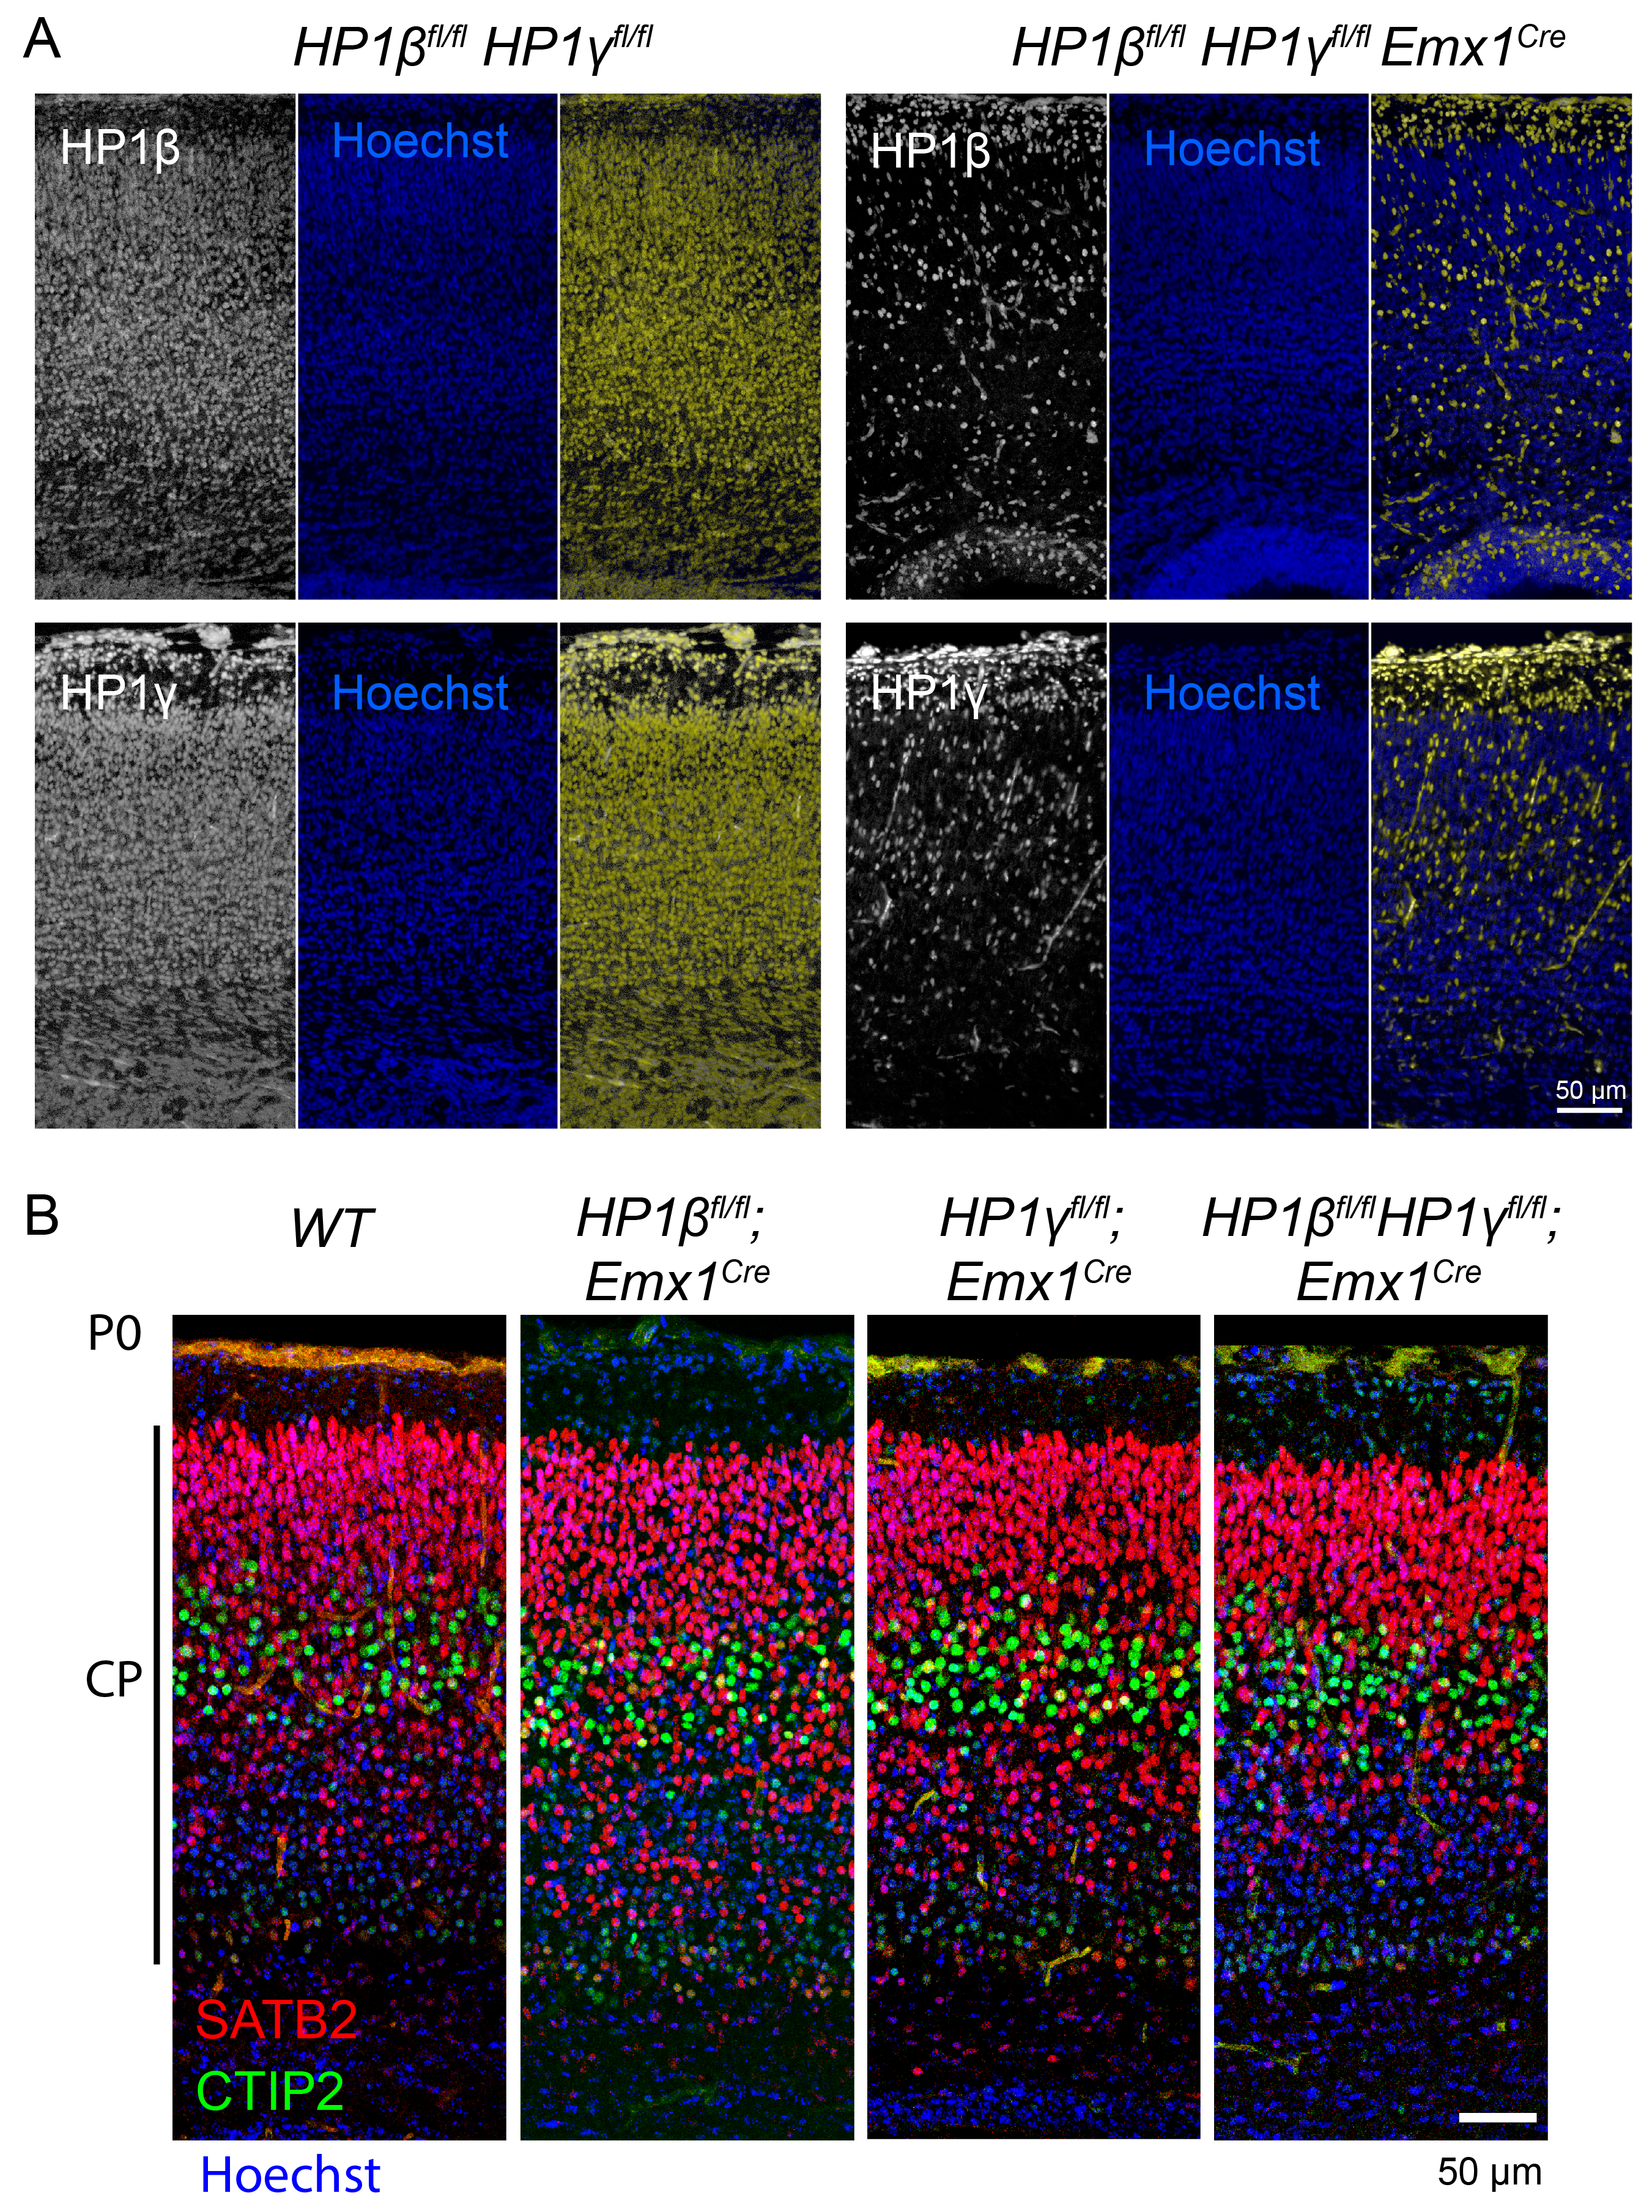
\includegraphics[width=1\linewidth, ]{./figure/results/FECctxHP1Bg} 
  
  }
  
  \caption[Emx1-Cre -Mediated Deletion of HP1 Proteins from the Cerebral Cortex.]{Emx1-Cre -Mediated Deletion of HP1 Proteins from the Cerebral Cortex.  (A): Staining of P0 somatosensory cortex reveals that HP1 proteins are deleted from pyramidal cells in the presence of Emx1-Cre. (B): Cell Fate and Laminarization is Unaffected in HP1$\beta$/$\gamma$ DKO Cortices. Specification of upper layer neurons marked by SATB2 and deep layer neurons marked by CTIP2 in the cortical plate (CP) is unperturbed following deletion of HP1$\beta$, HP1$\gamma$, or both.}\label{fig:FECctx}
  \end{figure}
  
  Surprisingly, cell fate and laminarization is unaffected in
  \emph{HP1\(\beta\)\textsuperscript{fl/fl}Emx1\textsuperscript{Cre}},
  \emph{HP1\(\gamma\)\textsuperscript{fl/fl}Emx1\textsuperscript{Cre}} and
  \emph{HP1\(\beta\)\textsuperscript{fl/fl}\(\gamma\)\textsuperscript{fl/fl}Emx1\textsuperscript{Cre}}
  cortices, as evidenced by normal distribution of upper layer neurons
  marked by SATB2 and deep layer neurons marked by CTIP2 (Figure
  \ref{fig:FECctx}B).
  
  Cells remaining positive for HP1\(\beta\) or HP1\(\gamma\) are negative
  for SATB2, and could be interneurons, epithelial or other cell types
  that are non- \emph{Emx1} lineage (Figure \ref{fig:Satb2exclude}).
  
  \begin{figure}
  
  {\centering 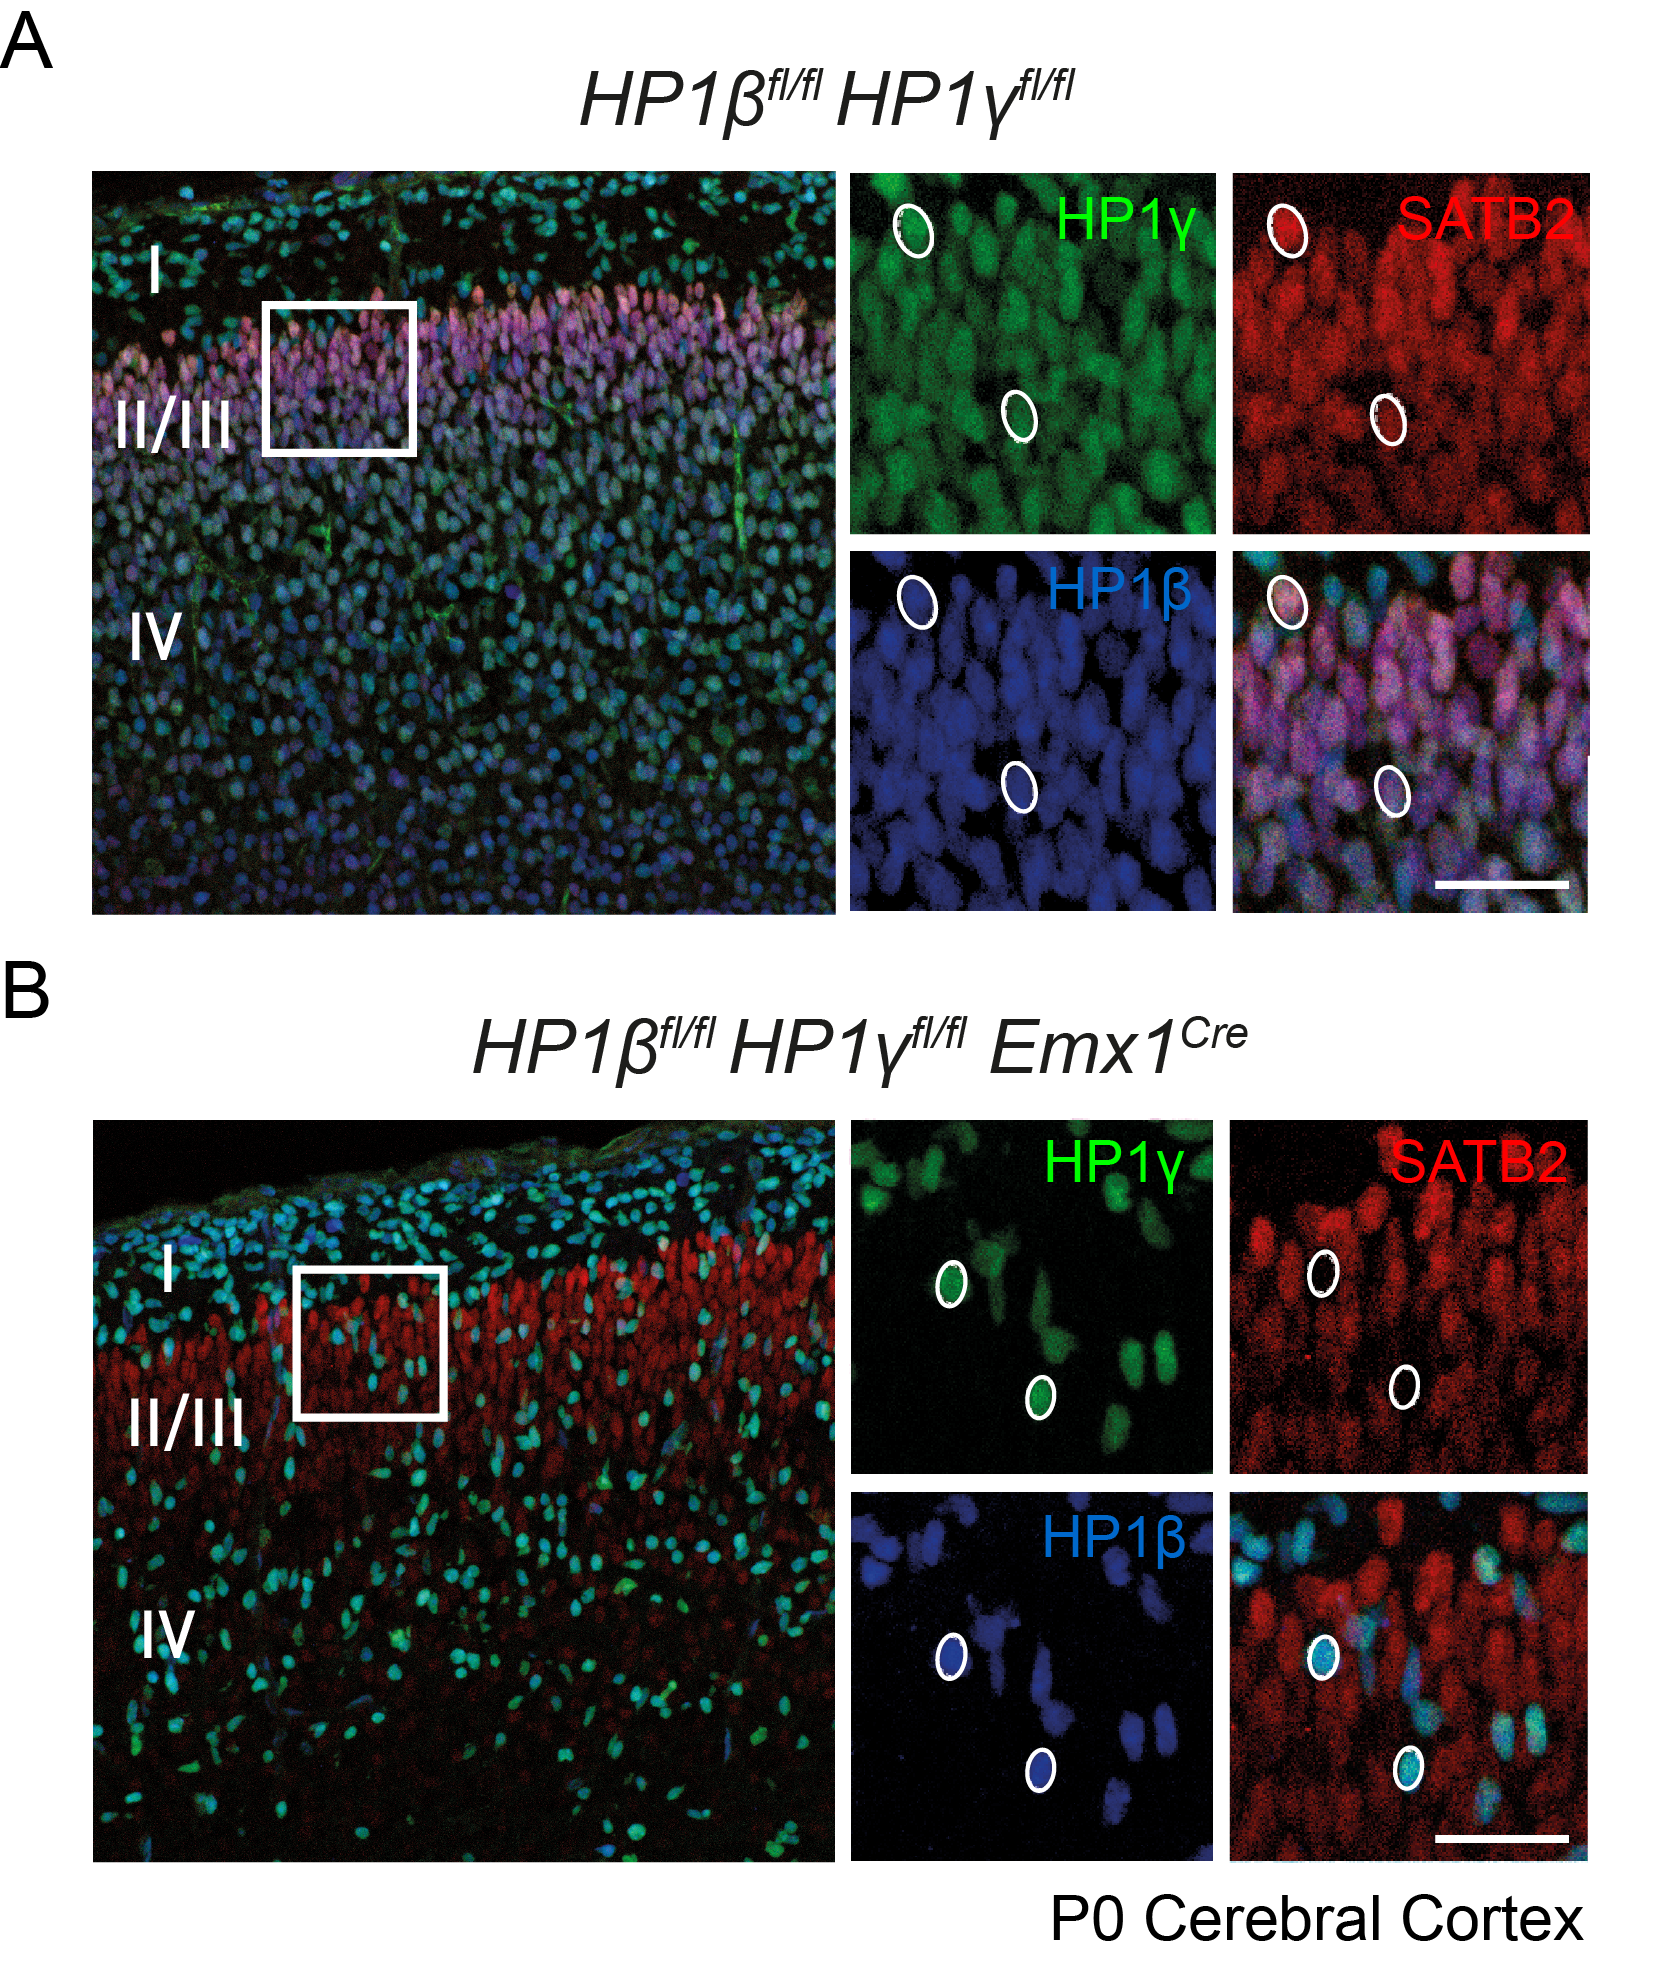
\includegraphics[width=1\linewidth, ]{./figure/results/FECCTXcellfate} 
  
  }
  
  \caption[Cells remaining positive for HP1 in HP1DKO cortex are of non-pyramidal lineage]{Cells in upper layers of the cerebral cortex remaining positive for HP1$\beta$ or HP1$\gamma$ in the HP1DKO mutant are negative for SATB2 (white circles), excluding them from pyramidal lineage. Scalebar = 25$\mu$m}\label{fig:Satb2exclude}
  \end{figure}
  
  \FloatBarrier
  
  \subsection{Imprinted Loci}\label{imprint}
  
  Given the known involvement of HP1 with the ZFP57-KAP1 repressive
  complex in controlling imprinted loci (Voon and Gibbons
  \protect\hyperlink{ref-VoonMaintainingmemorysilencing2016}{2016}), the
  expression of several imprinted loci was profiled by in situ
  hybridization. While some imprinted genes maintain expression in mature
  neurons such as \emph{Plagl1}, no differences could be detected in HP1
  mutants at P0 (Figure \ref{fig:Plagl1}). Additionally, probes designed
  for canonically imprinted \emph{Impact}, \emph{Inpp5f}, \emph{Gnas},
  \emph{Grb10}, \emph{Mdga1}, \emph{Rasgrf1} or \emph{Pip5k1c} did not
  reveal any changes in tissue expression following single or double
  deletion of HP1 proteins in the \emph{Emx1} lineage (data not shown).
  
  \begin{figure}
  
  {\centering \includegraphics[width=1\linewidth, ]{./figure/results/Plagl1} 
  
  }
  
  \caption[Imprinted Loci Are unaffected in HP1 Mutants at P0]{Imprinted Loci Are unaffected in HP1 Mutants at P0.  Shown here is the in situ-hybridization signal for Plagl1.}\label{fig:Plagl1}
  \end{figure}
  
  \section{Perturbed Regulation of Retroelements in HP1
  Mutants}\label{perturbed-regulation-of-retroelements-in-hp1-mutants}
  
  Given the known association of HP1 proteins with the KAP1 repressive
  complex and its role in silencing repetitive elements, I hypothesized
  that their absence may affect the normal regulation of repetitive
  elements. To examine this in the brain, I designed consensus RNA probes
  to detect all copies of a particular retrotransposon by \emph{in situ
  hybridization} (ISH).
  
  \subsection{LINE1}\label{line1}
  
  An RNA probe designed against a 700 bp region of open reading frame 2
  (ORF2) of LINE1 revealed robust, ubiquitous expression in post-mitotic
  neurons of the cortex and hippocampus in both wild-type and mutant
  (Figure \ref{fig:LINEish}). While high expression in the dentate gyrus
  is concordant with the large body of work examining LINE-driven somatic
  mosaicism there (McConnell et al.
  \protect\hyperlink{ref-McConnellMosaiccopynumber2013}{2013}; Muotri et
  al. \protect\hyperlink{ref-MuotriEnvironmentalinfluenceL12009}{2009};
  Thomas, Paquola, and Muotri
  \protect\hyperlink{ref-ThomasLINE1RetrotranspositionNervous2012}{2012}),
  it was surprising to observe such high abundance of transcripts in all
  post-mitotic neurons of the cortex. Given such abundance in wild-type,
  it was not feasible to discern any changes in LINE transcription in HP1
  mutant brains by ISH. Notably, in the hippocampus, LINE1 expression is
  evident in the dentate gyrus as well as CA1 and CA3 fields.
  
  \begin{figure}
  
  {\centering \includegraphics[width=1\linewidth, ]{./figure/results/LINEish} 
  
  }
  
  \caption[In Situ Hybridization for LINE1 ORF2 in Adult Wildtype and HP1DKO Brains]{In Situ Hybridization for LINE transcripts in adult wild-type and HP1 $\beta$/$\gamma$ DKO brains.  LINE transcripts are already highly abundant in wild-type  post-mitotic neurons.}\label{fig:LINEish}
  \end{figure}
  
  \FloatBarrier
  
  \subsection{Class III ERVs}\label{class-iii-ervs}
  
  To examine possible dysregulation of Class III murine endogenous
  retroviruses, I designed a 450bp consensus probe to test all transcripts
  derived from MERVL-MT2, a murine ERVL/Class III endogenous retrovirus.
  The probe for MERVL that would hybridize to RNA transcripts originating
  from approximately \textasciitilde{}205 MERVL loci. MERVL-derived
  transcripts are important at the 2 cell (2C) stage of embryonic
  development and both their standalone expression and of MERVL-derived
  chimeras is tightly associated with naive pluripotency (Macfarlan et al.
  \protect\hyperlink{ref-MacfarlanEmbryonicstemcell2012}{2012}). Modest
  expression of MERVL derived transcripts can be observed in wild-type
  brains, and similar levels could be observed in HP1 mutants (Figure
  \ref{fig:MERVLish}).
  
  \begin{figure}
  
  {\centering \includegraphics[width=1\linewidth, ]{./figure/results/MERVL} 
  
  }
  
  \caption[In Situ Hybridization Using a Consensus Probe for MERVL]{In Situ Hybridization Using a Consensus Probe for MERVL.  A probe was designed around a consensus sequence common to all MERVL elements.  MERVL transcripts appear unaltered in HP1 mutant brains.}\label{fig:MERVLish}
  \end{figure}
  
  \FloatBarrier
  
  \subsection{Class II ERVs}\label{class-ii-ervs}
  
  To examine possible dysregulation of Class II endogenous retroviruses, I
  designed a consensus probe for Intracisternal Alpha Particle (IAP), an
  evolutionary recent murine endogenous retrovirus of the ERVK family. To
  meet this end I created an RNA probe for a section of the \emph{gag}
  domain of IAP. A BLAST query predicted that such a sequence would
  hybridize to RNA transcripts originating from at least
  \textasciitilde{}196 IAP loci. While IAP transcripts are normally
  silenced in both wild-type and single mutant brains, a robust
  de-repression of IAP elements could be observed in the
  HP1\(\beta\)/\(\gamma\) double mutant (Figure \ref{fig:IAPcons}).
  
  \begin{figure}
  
  {\centering 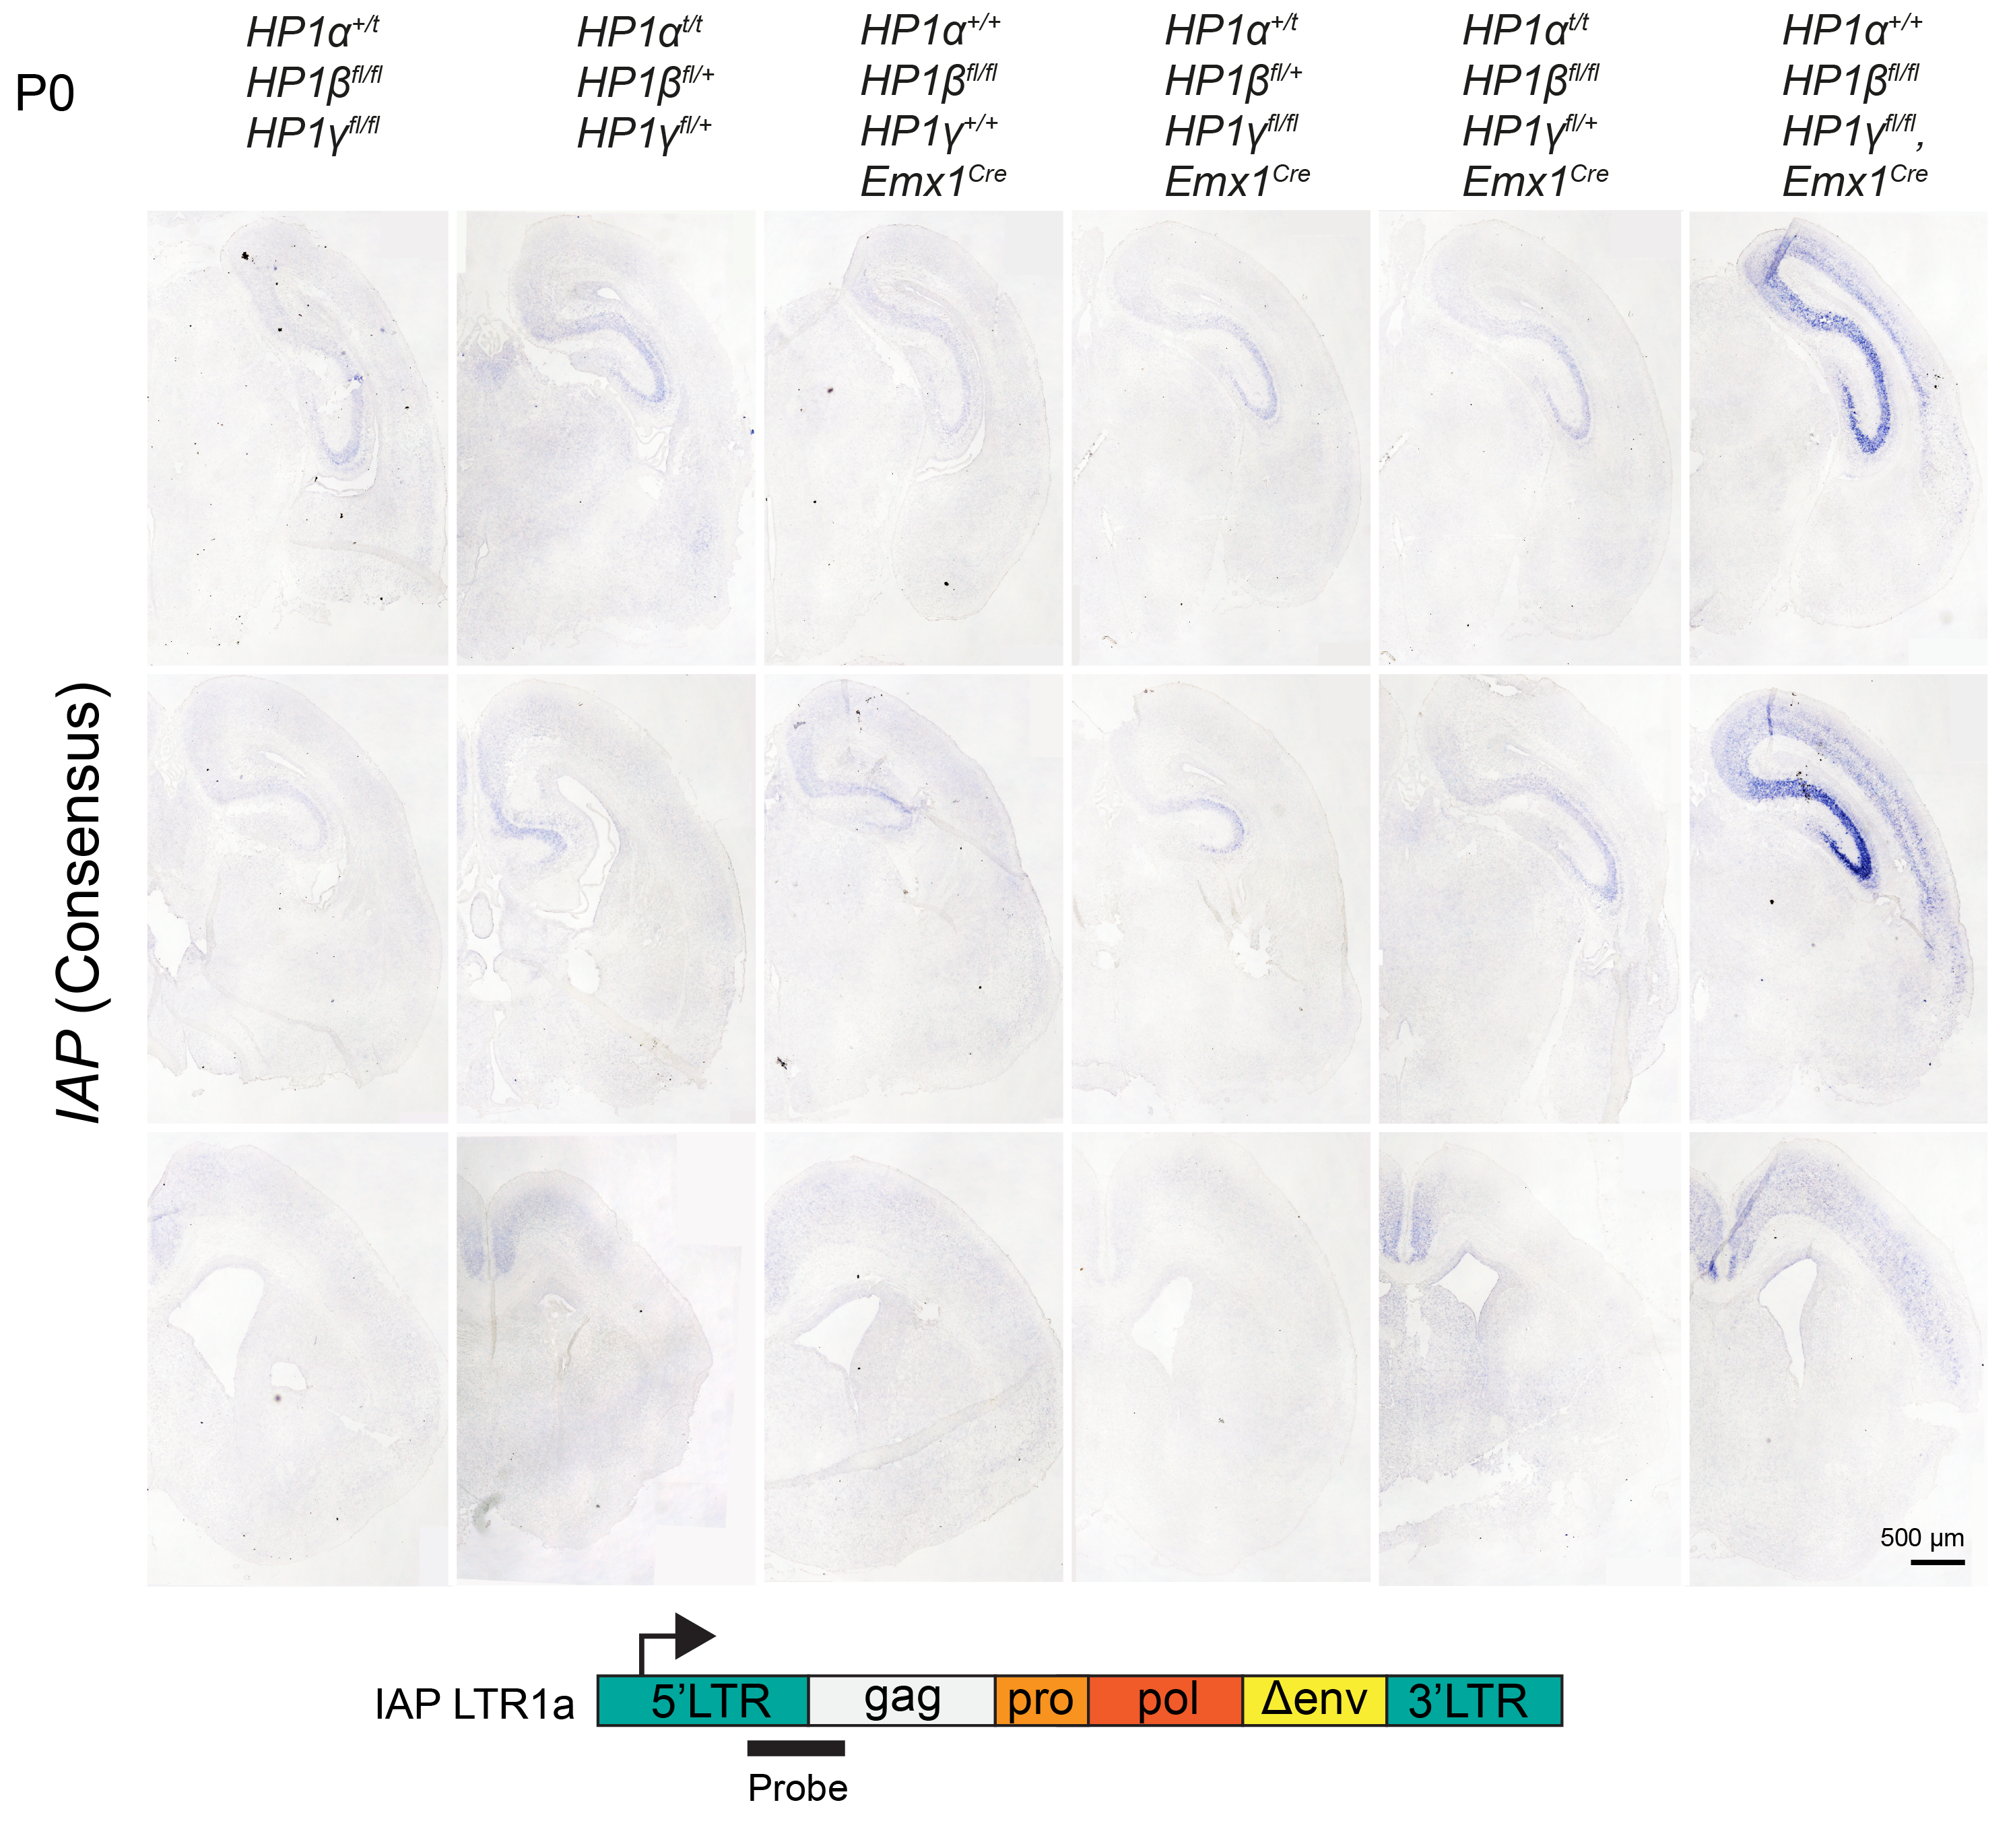
\includegraphics[width=1\linewidth, ]{./figure/results/IAPcons} 
  
  }
  
  \caption[Intracisternal Alpha Particle (IAP) elements are de-repressed in HP1$\beta$/$\gamma$ DKO]{Intracisternal Alpha Particle (IAP) elements are de-repressed in HP1$\beta$/$\gamma$ DKO.  In situ hybridization on various HP1 mutants using an RNA probe for a sequence common to IAP familly members.  IAP transcripts are strongly de-repressed in HP1$\beta$/$\gamma$ DKO, especially in the hippocampus.}\label{fig:IAPcons}
  \end{figure}
  
  \FloatBarrier
  
  To ensure the signal observed by the consensus probe was only
  hybridizing to IAP elements, I designed a separate probe that recognized
  a unique sequence on an IAP element found on chromosome 2. This RNA
  probe for a unique IAP sequence recapitulated the findings observed with
  the consensus probe, where robust de-repression could be observed in
  post-mitotic neurons of the cerebral cortex and hippocampus (Figure
  \ref{fig:IAPchr2}). IAP de-repression was confirmed to continue into
  adulthood (\ref{fig:IAPadult}), where it can be clearly observed that
  IAP de-repression in the hippocampus is restricted to CA1 and CA3 fields
  and absent from the dentate gyrus. This is a notable contrast from the
  expression of LINE1, which can be normally observed in all pyramidal
  fields of the hippocampus (Figure \ref{fig:LINEish}). Differences in
  cortical thickness in caudal portions of HP1DKO animals are addressed in
  section \ref{MRIresults}.
  
  \begin{figure}
  
  {\centering \includegraphics[width=1\linewidth, ]{./figure/results/IAPchr2} 
  
  }
  
  \caption[ISH of Unique IAP Element]{ISH of unique IAP Element on P0 brains.  A probe designed around a unique region on an evolutionary recent IAP element on chromosome 2 confirms specificity of the IAP consensus probe.}\label{fig:IAPchr2}
  \end{figure}
  
  \begin{figure}
  
  {\centering 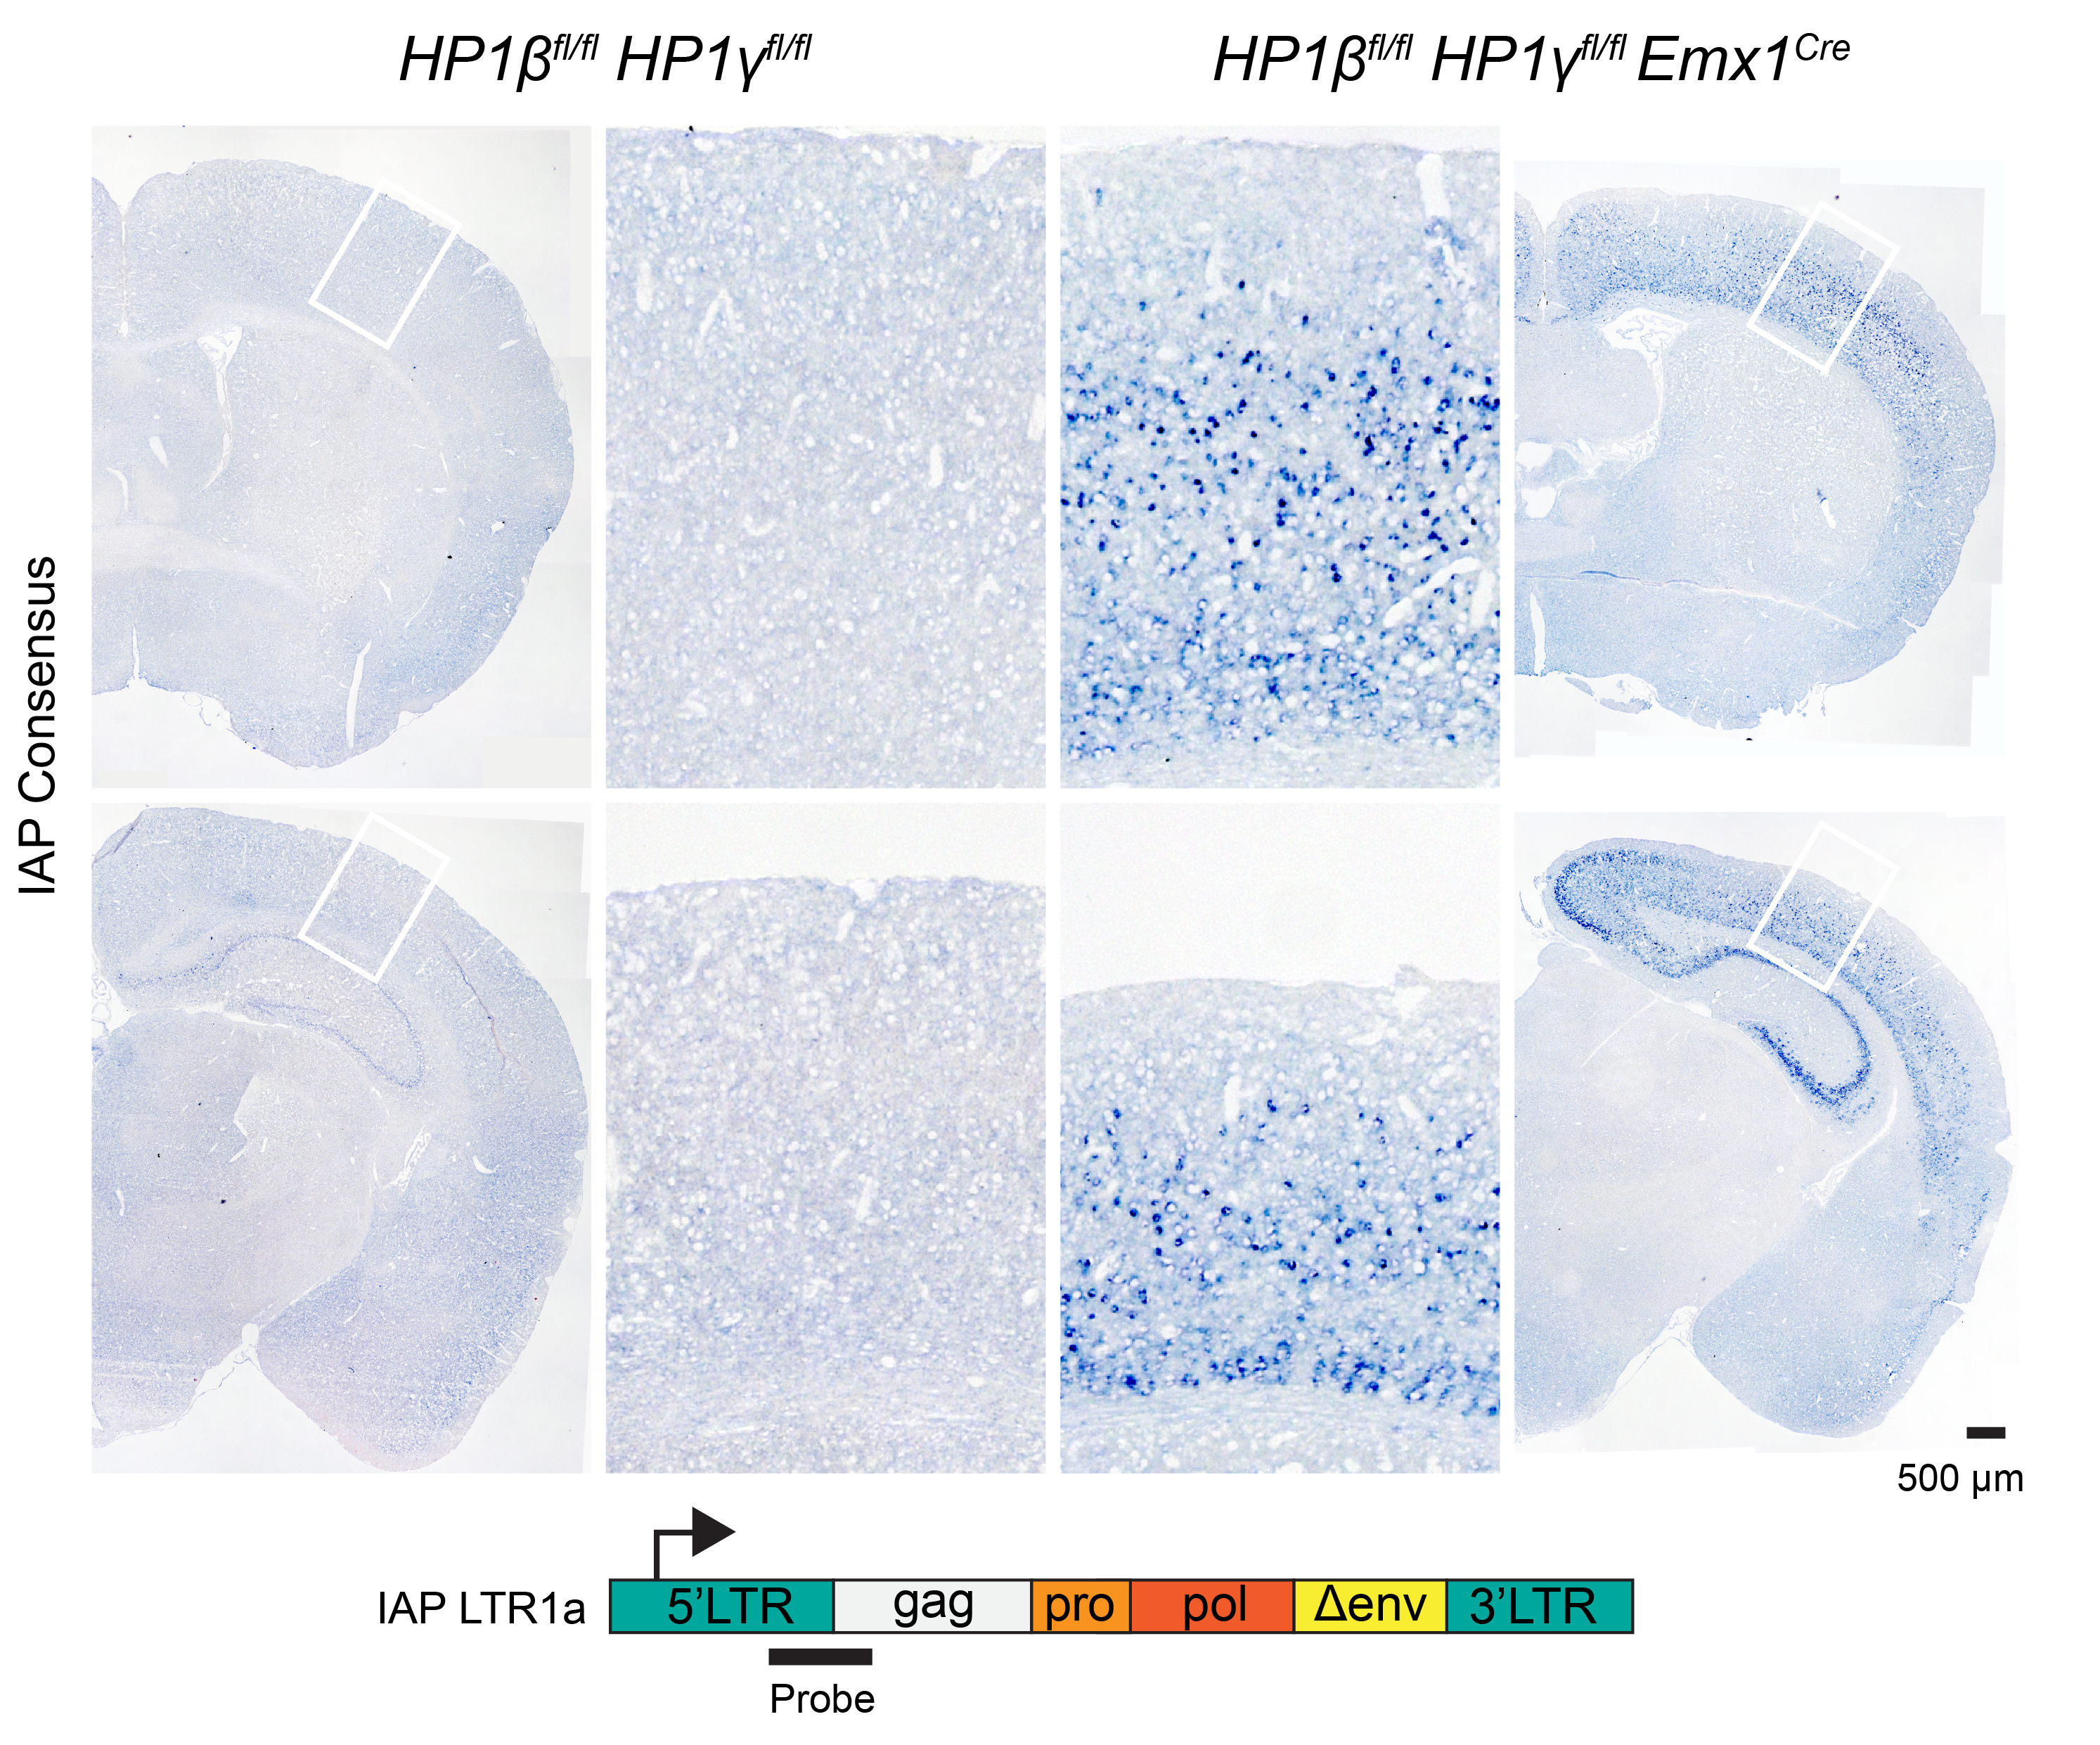
\includegraphics[width=1\linewidth, ]{./figure/results/IAPadult} 
  
  }
  
  \caption[Sustained IAP De-Repression in the Adult HP1β/γ DKO Brain]{Sustained IAP De-Repression in the Adult HP1β/γ DKO Brain. In situ hybridization using the IAP consensus probe in 3 month old adult brains.}\label{fig:IAPadult}
  \end{figure}
  
  \FloatBarrier
  
  \subsection{\texorpdfstring{\emph{De Novo}
  Retrotransposition}{De Novo Retrotransposition}}\label{de-novo-retrotransposition}
  
  Given multiple full-length copies of IAP elements capable of autonomous
  retrotransposition exist in the mouse (Dewannieux et al.
  \protect\hyperlink{ref-DewannieuxIdentificationautonomousIAP2004}{2004};
  Maksakova et al.
  \protect\hyperlink{ref-MaksakovaRetroviralElementsTheir2006}{2006};
  Saito et al.
  \protect\hyperlink{ref-SaitoTranslationnonautonomoustype2008}{2008}), I
  sought to determine if rates of \emph{de novo} transpositions were
  increased in HP1 mutant brains where IAP elements are de-repressed.
  Namely, do a subset of the IAP transcripts we observe encode for
  full-length autonomous retrotransposons? To examine this, GFP sensors
  encoding autonomous and non-autonomous IAP elements (pFL and pDE1
  respectively, Figure \ref{fig:IAPsensors}, (Horie et al.
  \protect\hyperlink{ref-HorieRetrotransposonsInfluenceMouse2007a}{2007}))
  were introduced by in utero electroporation (IUE) into wild-type and HP1
  mutant cortices (Figure \ref{fig:IAPIUE}).
  
  \begin{figure}
  
  {\centering \includegraphics[width=0.8\linewidth, ]{./figure/results/IAPsensors} 
  
  }
  
  \caption[Autonomous and Non-Autonomous IAP Sensors used to detect De Novo Retrotransposition. (Adapted from Horie et al., 2007)]{Autonomous and Non-Autonomous IAP Sensors used to detect De Novo Retrotransposition. (Top): The pFL plasmid encodes a full length IAP element followed by an antisense GFP containing an intron.  This construct can autonomously integrate into the genome, and will only express GFP upon integration and is thus an autonomous retrotransposon. The pDE1 plasmid encodes an IAP element with an internal deletion rendering it incapable to retrotranspose on its own (it is nonautonomous).  In the presence of a functional (autonomous) IAP provided in trans, retrotransposition of pDE1 can be made possible. (Bottom): Only following successful transcription, splicing and genomic integration can GFP be expressed, thus the presence of GFP informs on de novo genomic integration(s).}\label{fig:IAPsensors}
  \end{figure}
  
  Following exogenous introduction of the autonomous IAP sensor (pFL),
  \emph{de novo} genomic integrations could be observed in both wild type
  and HP1\(\beta\)/\(\gamma\) DKO cortices with similar frequencies
  (Figure \ref{fig:IAPIUE}A). While introduction of the defunct IAP sensor
  pDE1 into wildtype never resulted in any integrations measured by GFP
  positive cells (n = 6), when introduced into HP1\(\beta\)/\(\gamma\) DKO
  cortex several integration events could be observed (Figure
  \ref{fig:IAPIUE}B).
  
  \begin{figure}
  
  {\centering \includegraphics[width=1\linewidth, ]{./figure/results/IAPIUE} 
  
  }
  
  \caption[De-Repressed IAP Transcripts Facilitate De Novo Retrotransposition in Trans ]{De-Repressed IAP Transcripts Facilitate De Novo Retrotransposition in Trans. Introduction by in utero electroporation (IUE) of autonomous and non-autonomous IAP integration sensors at E14 and observed at E18.  The introduction of a non-autonomous IAP pDE1 into wildtype does not result in integration, however integrations can be observed when introduced into HP1$\beta$/$\gamma$ DKO brains, where IAP elements are de-repressed.  Because pDE1 requires the presence of a functional IAP for genomic integration, this infers a subset of IAP elements de-repressed in the HP1$\beta$/$\gamma$ DKO are functionally autonomous retrotransposons.}\label{fig:IAPIUE}
  \end{figure}
  
  \FloatBarrier
  
  \section{\texorpdfstring{Sustained HP1\(\beta\)/\(\gamma\) Deficiency
  Adversely Affects Neuronal Complexity, Function and
  Cognition}{Sustained HP1\textbackslash{}beta/\textbackslash{}gamma Deficiency Adversely Affects Neuronal Complexity, Function and Cognition}}\label{sustained-hp1betagamma-deficiency-adversely-affects-neuronal-complexity-function-and-cognition}
  
  The
  \emph{HP1\(\beta\)\textsuperscript{fl/fl}HP1\(\gamma\)\textsuperscript{fl/fl}Emx1\textsuperscript{Cre}}
  mutants provided an interesting model. While neuronal differentiation
  proceeds relatively normally -at least in terms of classical identity,
  HP1 double mutants exhibit precocious de-repression of endogenous
  retroviruses, a phenotype that emerges gradually with normal aging. The
  question was then posed ``What is the functional consequence to the
  organism when sustained de-repression of such elements occurs in
  neurons?'' To answer this, behavioral phenotyping was performed in
  addition to descriptive volumetrics and histology.
  
  \subsection{Behavior}\label{behavior}
  
  \subsubsection*{\texorpdfstring{\emph{Seizures}}{Seizures}}\label{seizures}
  \addcontentsline{toc}{subsubsection}{\emph{Seizures}}
  
  Upon initial handling, it was observed that many HP1FEC animals
  descended into brief tonic-clonic seizures following novel stimulus,
  such as a cage change or routine handling. Such seizures typically
  included a violent convulsion stage lasting about 5 seconds, where in
  the most extreme cases included excessive salivation. Such convulsions
  were followed by a 15-30 second period of stupor where the animal was
  non-responsive. Following this period of stupor, animals exhibited
  entirely normal behavior. After these initial observations, I installed
  a seizure log where seizures could be documented by animal staff and
  myself. Seizures were recorded from April 2015 until February 2017
  (Figure \ref{fig:seizures}). While seizures occurred primarily in
  HP1\(\beta\) animals, some were observed in the other genotypes. It
  should be noted that because these observations rely on animal staff
  reporting the correct earcode of the animal, rather than a concrete
  genotype, it is possible that some observations were inaccurately
  reported, such as those seen in wildtype.\\
  
  \begin{figure}
  
  {\centering \includegraphics[width=1\linewidth, ]{./figure/results/seizures} 
  
  }
  
  \caption[Seizures in HP1 Mutants]{Seizures in HP1 Mutants.  Seizures were documented in HP1FEC animals in their home cages in the animal facility as well as those undergoing behavioral testing. }\label{fig:seizures}
  \end{figure}
  
  Several behavioral tests were used to test for alterations to
  exploratory behavior, anxiety, and learning and memory in young and aged
  HP1FEC animals. Young (3 months) and Aged (13-14 months) male mice were
  tested in \emph{Open Field Activity}, \emph{Cued Context Fear Learning},
  \emph{Paired-Pulse Inhibition}, the \emph{Barnes Maze}, \emph{Social
  Activity Monitor}, \emph{HomeCageScan} and \emph{Nest Construction}.
  Detailed results of \emph{HomeCageScan} and \emph{Cued Context Fear
  Learning} can be found in Appendix \ref{Behavsupplement}. Prior to all
  behavioral phenotyping, animals were assessed using a modified SHIRPA to
  ensure animals did not have any physical limitations that could bias
  behavioral testing, such as deficits in vision, audition, grip strength
  or locomotion. A total of 42 animals (15 WT, 11 HP1\(\beta\)KO, 6
  HP1\(\gamma\)KO, 10 HP1\(\beta\)/\(\gamma\)DKO) completed the aged time
  point, where 4 died (2 WT, 1 HP1\(\beta\)KO, 1
  HP1\(\beta\)/\(\gamma\)DKO) between young and aged testing. All of the
  following box and whisker plots are comprised of median and
  25\textsuperscript{th} and 75\textsuperscript{th} percentiles, where
  whiskers extend no further than 1.5X the interquartile range. All line
  charts plot the mean and standard error as a ribbon surrounding the
  line.
  
  \FloatBarrier
  
  \subsubsection*{\texorpdfstring{\emph{Open Field
  activity}}{Open Field activity}}\label{open-field-activity}
  \addcontentsline{toc}{subsubsection}{\emph{Open Field activity}}
  
  Anxiety and exploration was measured using a simple open field test,
  where animals are placed in the center of a square open field and their
  activity in both the center and the periphery is tracked over the course
  of 10 minutes (Figure \ref{fig:openfield}).
  
  In young animals, significant decreases in average ambulation velocity
  and percent activity were observed in HP1\(\beta\)KO animals. This
  effect was due primarily to a strong initial freezing response in
  roughly half of the HP1\(\beta\) animals following entrance of the
  animal into the center of the arena at the beginning of the test. This
  initial freezing response in HP1\(\beta\)KO animals was akin to
  non-convulsive status epilepticus rather than a fear response. Typically
  midway through the test HP1\(\beta\) animals began normal exploration
  and avoidance of the center. In aged animals, the initial freezing
  response could be observed in a subset of HP1\(\beta\)KO animals,
  however the strongest effect was seen in aged DKO animals, where a
  majority showed a prolonged stupor in the center of the open field at
  the beginning of the test.
  
  \begin{figure}
  
  {\centering \includegraphics[width=1\linewidth, ]{./figure/results/Open_field} 
  
  }
  
  \caption[Open Field Activity in HP1 Mutants]{Open Field Activity in HP1 Mutants. Ribbons surrounding per-minute line plots denote SEM. Statistics: two-way ANOVA with bonferroni corrections on multiple comparisons. Asterisks (*) denote tests within age for differences between genotype: *** = p < 0.001, ** = p < 0.01, * = p < 0.05. All statistically significant changes associated with age within genotype are represented by a pound sign (\#): \#\#\# = p < 0.001,  \#\# = p < 0.01, \# = p < 0.05).}\label{fig:openfield}
  \end{figure}
  
  \subsubsection*{\texorpdfstring{\emph{Social Activity Monitor
  (SAM)}}{Social Activity Monitor (SAM)}}\label{social-activity-monitor-sam}
  \addcontentsline{toc}{subsubsection}{\emph{Social Activity Monitor
  (SAM)}}
  
  To examine social activity and circadian rhythm, animal activity was
  measured in their home cages by RFID chip movement. Animals were
  monitored over 14 days and data was averaged first within animal by hour
  of the day across all days, then by genotype (Figure \ref{fig:SAM}).
  
  \begin{figure}
  
  {\centering \includegraphics[width=0.85\linewidth, ]{./figure/results/SAMalt} 
  
  }
  
  \caption[Social Activity of HP1 mutants by Time of Day]{Social Activity of HP1 mutants by Time of Day.  The activity of each animal was recorded over a 14-day period.  Individual animal activity was averaged by each hour of the day over the duration, then grouped by genotype and age.  Plotted here is the mean activity per hour (thick line) along with the standard error of the mean (ribbon) per genotype by age.  Statistics: two-way ANOVA with bonferroni corrections on multiple comparisons. Asterisks (*) denote tests within age for differences between genotype: *** = p < 0.001, ** = p < 0.01, * = p < 0.05. All statistically significant changes associated with age within genotype are represented by a pound sign (\#); (\#\#\# = p < 0.001, \#\# = p < 0.01, \# = p < 0.05).}\label{fig:SAM}
  \end{figure}
  
  \FloatBarrier
  
  \subsubsection*{\texorpdfstring{\emph{HomeCageScan \& Animal
  Microbehaviors}}{HomeCageScan \& Animal Microbehaviors}}\label{homecagescan-animal-microbehaviors}
  \addcontentsline{toc}{subsubsection}{\emph{HomeCageScan \& Animal
  Microbehaviors}}
  
  Following a 24 hr observation period under active scanning, the
  frequency and number of discrete bouts of various microbehaviors was
  quantified. These behaviors are summarized in supplemental Figures
  \ref{fig:HCSpie}, \ref{fig:HCSpercent} and \ref{fig:HCSbouts}. Several
  behaviors associated with increased anxiety could be observed in
  HP1\(\gamma\) and HP1 double mutants. Notable changes were observed in
  both the bouts and percent of time spent grooming in HP1\(\gamma\) and
  HP1DKO young mice, which is sustained with age (Figure
  \ref{fig:GroomEatWeight}A-B). Additionally, aged HP1DKO animals spend
  significantly more time eating (Figure \ref{fig:GroomEatWeight}C-D),
  which corresponds to a tendency for the HP1DKOs to gain weight (Figure
  \ref{fig:GroomEatWeight}E).
  
  \begin{figure}
  
  {\centering \includegraphics[width=1\linewidth, ]{./figure/results/GroomEatWeight} 
  
  }
  
  \caption[HP1 $\beta$/$\gamma$ DKO Mutants Display Microbehaviors associated with increased Anxiety]{HP1 $\beta$/$\gamma$ DKO Mutants Display Microbehaviors associated with increased Anxiety. Statistics: two-way ANOVA with bonferroni corrections on multiple comparisons. Asterisks (*) denote tests within age for differences between genotype: *** = p < 0.001, ** = p < 0.01, * = p < 0.05. All statistically significant changes associated with age within genotype are represented by a pound sign (\#); (\#\#\# = p < 0.001, \#\# = p < 0.01, \# = p < 0.05).}\label{fig:GroomEatWeight}
  \end{figure}
  
  \FloatBarrier
  
  \subsubsection*{\texorpdfstring{\emph{Paired-Pulse
  Inhibition}}{Paired-Pulse Inhibition}}\label{paired-pulse-inhibition}
  \addcontentsline{toc}{subsubsection}{\emph{Paired-Pulse Inhibition}}
  
  An examination for alterations in paired-pulse inhibition revealed an
  age-dependent deficit in HP1DKO animals (Figure \ref{fig:PPI}). While
  all aged animals displayed a tendency towards weaker paired-pulse
  inhibition, aged HP1DKO animals showed little change in startle response
  with increasing amplitude of pre-pulse.
  
  \begin{figure}
  
  {\centering \includegraphics[width=1\linewidth, ]{./figure/results/PPI} 
  
  }
  
  \caption[Percent Paired-Pulse Inhibition In HP1 Mutants]{Percent Paired-Pulse Inhibition In HP1 Mutants.  Percent paired-pulse inhibition was measured by percent normalizing the measured startle responses in each pre-pulse condition (69 dB, 71 dB and 81 dB) to the measured startle response to the pulse (120 dB). Statistics: two-way ANOVA with bonferroni corrections on multiple comparisons. Asterisks (*) denote tests within age for differences between genotype: *** = p < 0.001, ** = p < 0.01, * = p < 0.05. All statistically significant changes associated with age within genotype are represented by a pound sign (\#); (\#\#\# = p < 0.001, \#\# = p < 0.01, \# = p < 0.05).}\label{fig:PPI}
  \end{figure}
  
  \FloatBarrier
  
  \subsubsection*{\texorpdfstring{\emph{Nest
  Construction}}{Nest Construction}}\label{nest-construction}
  \addcontentsline{toc}{subsubsection}{\emph{Nest Construction}}
  
  Pilot experiments revealed that following the two day separation of male
  animals from their homecages, return to their homecage resulted in
  excessive aggression and violence between former cohabitants. For this
  reason the nest construction test was only tested at the aged timepoint.
  Nest construction was adversely affected in HP1DKO mutants both in terms
  of complexity (complexity score, methods \ref{nestcomethod}) and
  completion (\% nestlet used in constructing the nest) (Figure
  \ref{fig:Nestconstruction}). In most cases, HP1DKO animals barely
  touched the cotton nestlet, leaving it mostly intact (Figure
  \ref{fig:Nestconstruction}C).
  
  \begin{figure}
  
  {\centering \includegraphics[width=1\linewidth, ]{./figure/results/Nest} 
  
  }
  
  \caption[Nest Construction Test]{Nest Construction and Complexity.  (A) plots the amount of nest construction, where any remaining solid nestlet is percent normalized to its initial weight.  Nest complexity is qualified in (B), which was measured using a standardized rubrick (see methods). (C) Representative images of nests constructed by each genotype. Statistics: one-way ANOVA with bonferroni corrections on multiple comparisons: *** = p < 0.001, ** = p < 0.01, * = p < 0.05.}\label{fig:Nestconstruction}
  \end{figure}
  
  \FloatBarrier
  
  \subsubsection*{\texorpdfstring{\emph{Barnes
  Maze}}{Barnes Maze}}\label{barnes-maze}
  \addcontentsline{toc}{subsubsection}{\emph{Barnes Maze}}
  
  Spatial memory of HP1 animals was tested using the Barnes maze (methods
  \ref{Barnesmeth}). Rather than employing a direct strategy, which would
  involve directly navigating to the perceived target hole, HP1DKO animals
  often employed serial search patterns. HP1DKO animals walked clockwise
  or counter-clockwise around the periphery of the Barnes maze checking
  every hole (Figure \ref{fig:barnes}A). Such poor performance coincided
  with a significantly longer latency to target and significant decreases
  in the number of correct visits to target (Figure \ref{fig:barnes}B,C).
  
  \begin{figure}
  
  {\centering \includegraphics[width=1\linewidth, ]{./figure/results/barnes} 
  
  }
  
  \caption[HP1 Mutant Performance in the Barnes Maze]{HP1 Mutant Performance in the Barnes Maze. Histograms and inset radar plots displaying mean headpokes +SEM per hole (A) reveal search patterns of HP1 mutants in each test by age.  Total percent correct visits (B) and latency to target (C) summarize effects by genotype. Statistics: two-way ANOVA with bonferroni corrections on multiple comparisons. Asterisks (*) denote tests between specified genotype and wildtype within age group: *** = p < 0.001, ** = p < 0.01, * = p < 0.05. All statistically significant changes associated with age within genotype are represented by a pound sign (\#); (\#\#\# = p < 0.001, \#\# = p < 0.01, \# = p < 0.05).}\label{fig:barnes}
  \end{figure}
  
  \FloatBarrier
  
  \subsection{Structure, Volumetrics and Histology}\label{MRIresults}
  
  Given strong behavioral deficits in spatial memory and the
  aforementioned strong de-repression of IAP elements in the developing
  hippocampus, further attention was paid to determine any alterations in
  hippocampal circuitry or structure.
  
  \subsubsection*{\texorpdfstring{\emph{Reduced Dendritic Complexity in
  Hippocampal CA3
  Neurons}}{Reduced Dendritic Complexity in Hippocampal CA3 Neurons}}\label{reduced-dendritic-complexity-in-hippocampal-ca3-neurons}
  \addcontentsline{toc}{subsubsection}{\emph{Reduced Dendritic Complexity
  in Hippocampal CA3 Neurons}}
  
  Dendritic complexity of CA3 neurons was quantified in young and aged HP1
  mutants by golgi impregnation (Figure \ref{fig:golgiquant}). Young CA3
  neurons from both HP1\(\beta\)KO and HP1DKO animals showed marked
  reduction in the complexity of their basal dendritic trees (Figure
  \ref{fig:golgiquant}C, E). This trend continues into aged animals, most
  prominently in HP1DKO animals, where a drastic loss of basal dendrite
  complexity can be observed (Figure \ref{fig:golgiquant}D, F).
  
  \begin{figure}
  
  {\centering \includegraphics[width=1\linewidth, ]{./figure/results/golgiCA3quant5} 
  
  }
  
  \caption[Dendritic Complexity of Hippocampal CA3 Neurons in Young and Aged HP1 Mutants]{Dendritic Complexity of Hippocampal CA3 Neurons in Young and Aged HP1 Mutants.  Dendritic complexity was quantified by golgi impregnation followed by Scholl analysis, where intersections of dendrites in each of thirty 10 $\mu$m concentric circles were quantified (A).  (B) displays representative reconstructions of CA3 neurons.  Scholl analysis is plotted for neurons from young (C) and aged animals (D) by genotype, where the thickness of the line corresponds with the standard error around the mean and n refers to the number of neurons counted accross 3 hippocampi from each condition.  Box and whisker plots display total apical and basal interactions for young (E) and aged (F) animals. Statistics: two-way ANOVA with bonferroni corrections on multiple comparisons. Asterisks (*) denote tests within age for differences between genotype: *** = p < 0.001, ** = p < 0.01, * = p < 0.05. All statistically significant changes associated with age within genotype are represented by a pound sign (\#); (\#\#\# = p < 0.001, \#\# = p < 0.01, \# = p < 0.05).}\label{fig:golgiquant}
  \end{figure}
  
  \subsubsection*{\texorpdfstring{\emph{Malformation of the Dentate
  Gyrus}}{Malformation of the Dentate Gyrus}}\label{malformation-of-the-dentate-gyrus}
  \addcontentsline{toc}{subsubsection}{\emph{Malformation of the Dentate
  Gyrus}}
  
  It became apparent that the infrapyramidal blade of the dentate gyrus
  was missing in HP1\(\beta\)KO and HP1DKO animals (Figure
  \ref{fig:nissl}). In order to understand this deficit, I stained for
  dividing cells (Ki-67) and post-mitotic granule neurons (Prox1) at early
  postnatal timepoints when the dentate gyrus is formed (Figure
  \ref{fig:prox1ki67}). At P0, HP1DKO dentate gyrii show a statistically
  significant decrease in Ki-67 positive cells, and already show a trend
  towards a decrease in Prox1 positive cells. By postnatal day 8,
  HP1\(\beta\)KO and HP1DKO animals fail to generate the granular and
  molecular layers of the infrapyramidal blade of the dentate gyrus, which
  corresponds with a decrease in total area, and in the number of Prox1
  positive and proliferative Ki-67 positive cells (Figure
  \ref{fig:prox1ki67}B \& C). Given that a subset of DG granule cells in
  the infrapyramidal blade project to the basal dendrites of CA3 cells, it
  is likely that dentate gyrus malformations seen in HP1\(\beta\)KO and
  HP1DKO animals are directly linked to the progressive loss of CA3 basal
  dendritic fields in those animals. It should also be noted that while
  the infrapyramidal blade of the dentate gyrus is lost in HP1\(\beta\)KO
  animals, they do not exhibit the same behavioral abnormalities seen in
  HP1\(\beta\)/\(\gamma\)DKO animals. \FloatBarrier
  
  \begin{figure}
  
  {\centering 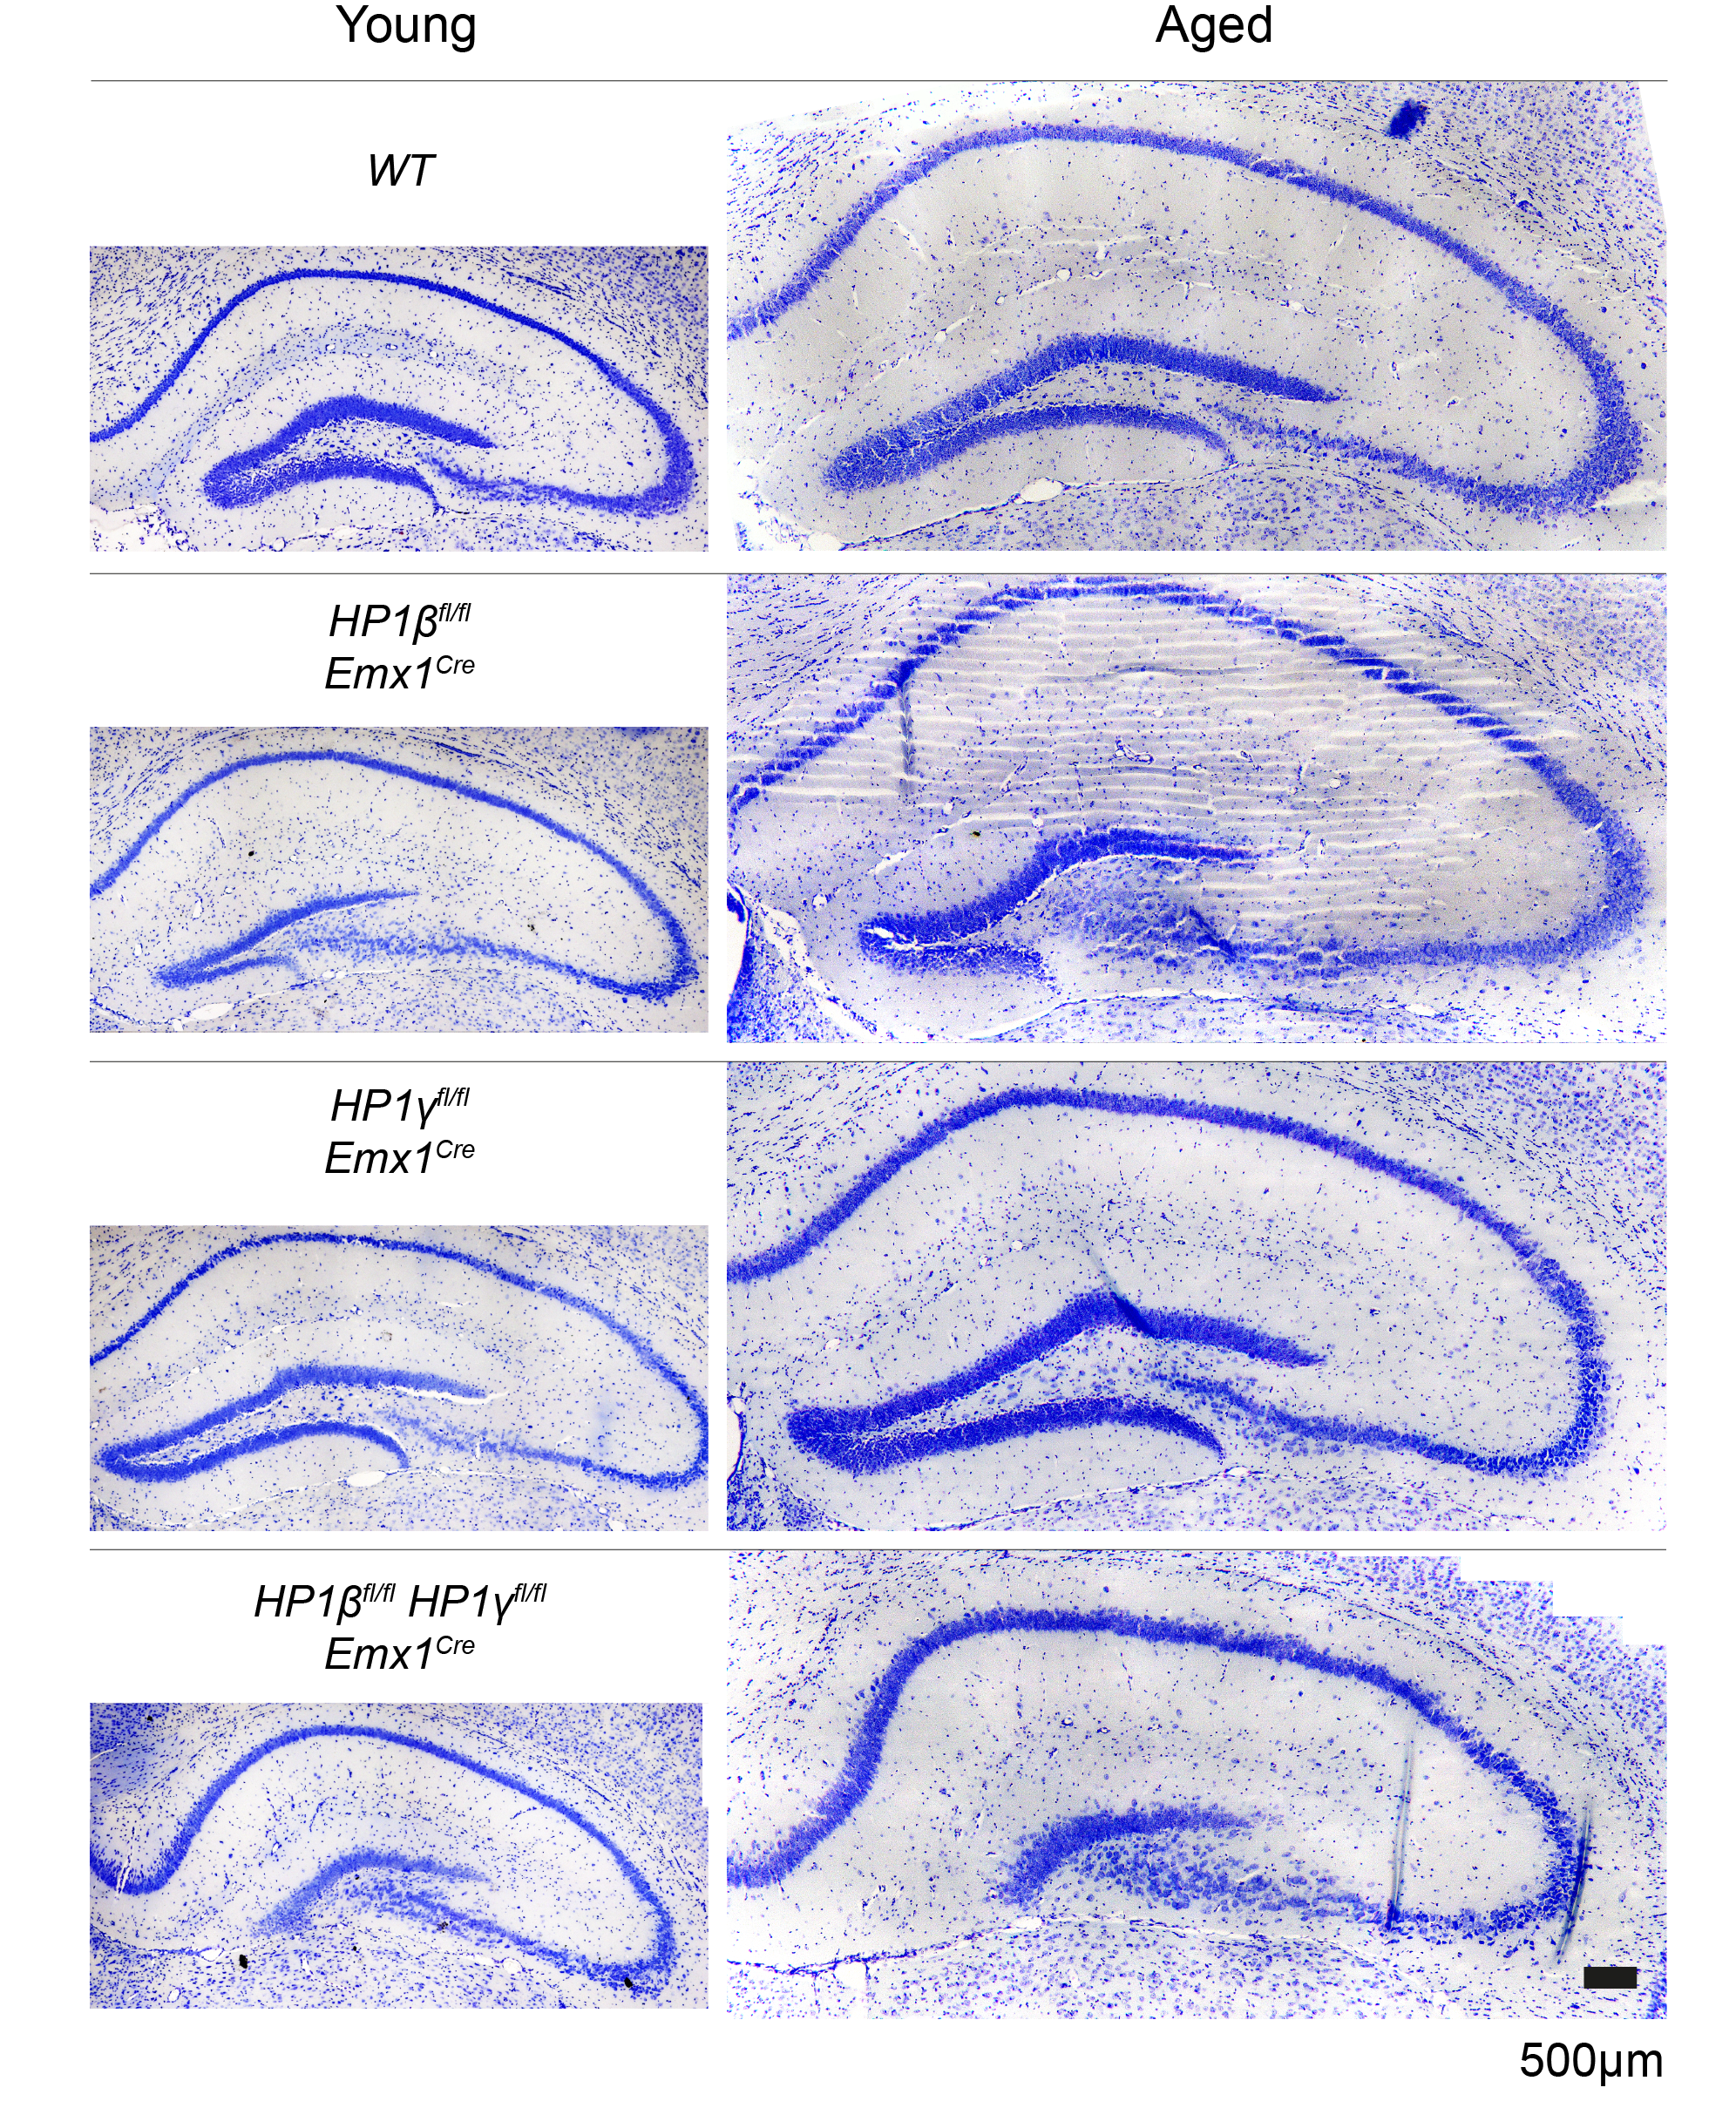
\includegraphics[width=1\linewidth, ]{./figure/results/_Nissl} 
  
  }
  
  \caption[Young and Aged Adult HP1 Mutant Hippocampi]{Young and Aged Adult HP1 Mutant Hippocampi. A nissl stain using cresyl violet on paraffin sections.}\label{fig:nissl}
  \end{figure}
  
  \begin{figure}
  
  {\centering \includegraphics[width=1\linewidth, ]{./figure/results/DGprox1ki67} 
  
  }
  
  \caption[Dentate Gyrus Malformations in HP1 Mutants]{Dentate Gyrus Malformations in HP1 Mutants. (A) Representative images of HP1 mutant dentate gyrii at postnatal day 0 (P0) and day 8 (P8) stained for Prox1, Ki-67 and DAPI. (B) Measured areas of dentate gyrii filling a standard field of view. (C) Plots Prox1 and Ki-67 positive cells by genotype.  Statistics: One-way ANOVA within age for area or marker with Dunnett's multiple comparison test. *** = p < 0.001, ** = p < 0.01, * = p < 0.05. P0: WT n = 10, HP1$\beta$KO n = 4, HP1$\gamma$KO n = 7, HP1DKO n = 11. P8: WT n = 4, HP1$\beta$KO n = 3, HP1$\gamma$KO n = 4, HP1DKO n = 5, where n is a biological replicate}\label{fig:prox1ki67}
  \end{figure}
  
  \FloatBarrier
  \clearpage
  
  \subsubsection*{\texorpdfstring{\emph{Volumetrics}}{Volumetrics}}\label{volumetrics}
  \addcontentsline{toc}{subsubsection}{\emph{Volumetrics}}
  
  A formal characterization of volumetric changes to the cortex and
  hippocampus in HP1 mutants was obtained by structural Magnetic Resonance
  Imaging (MRI). A notable reduction in the volume of the total brain,
  isocortex, hippocampal region and dentate gyrus was confirmed in HP1DKO
  animals (Figure \ref{fig:MRIresults}). As previously reported (Aucott et
  al. \protect\hyperlink{ref-AucottHP1requireddevelopment2008}{2008}), the
  constitutive deletion of \emph{HP1\(\beta\)} results in mitotic
  deficits, suggesting that while cells deficient for HP1\(\beta\) can
  divide, they have a finite number of divisions that can occur. In the
  \emph{Emx1\textsuperscript{Cre}} mouse line, Cre is expressed coincident
  with \emph{Emx1}, which begins at E10.5. Normally, the radial glia and
  subsequent intermediate progenitors undergo a finite amount of divisions
  in generating the post-mitotic neurons of the cortex and hippocampus.
  Given the dentate gyrus is one of the last regions to be formed, it
  stands to reason that HP1\(\beta\)-deficient neural progenitors
  prematurely exhaust their division potential. In parallel to DG loss,
  when normalizing to overall brain volume, young animals show specific
  reductions in slices 10 \& 11, which corresponds to the parietal and
  somatosensory cortices surrounding the hippocampus, and also that seen
  in Figure \ref{fig:IAPadult}. Notably, when normalized to total brain
  volume, cortical volumes are not statistically different from wildtype.
  
  \begin{figure}
  
  {\centering \includegraphics[width=1\linewidth, ]{./figure/results/_MRI} 
  
  }
  
  \caption[Volumetric Analysis of HP1 mutant brains by Magnetic Resonance Imaging]{Volumetric Analysis of HP1 mutant brains by Magnetic Resonance Imaging. (A) Representative MRI volume reconstructions with isocortex (cyan), hippocampus (green) and dentate gyrus (red) region masks applied. Total volume of the brain (B), hippocampus (C), dentate gyrus (D) and detailed analysis of the volume of the isocortex (E) is plotted by genotype for both ages. Ribbons around line plots in (E) account for standard deviation per slice per genotype. Statistics: one-way ANOVA within age with Bonferroni multiple comparison corrections. *** = p < 0.001, ** = p < 0.01, * = p < 0.05.}\label{fig:MRIresults}
  \end{figure}
  
  \FloatBarrier
  
  \section{\texorpdfstring{HP1\(\beta\) and HP1\(\gamma\) Synergistically
  Contribute to Repeat
  Silencing}{HP1\textbackslash{}beta and HP1\textbackslash{}gamma Synergistically Contribute to Repeat Silencing}}\label{hp1beta-and-hp1gamma-synergistically-contribute-to-repeat-silencing}
  
  The robust de-repression of ERVs in HP1\(\beta\)/\(\gamma\) DKO cells is
  in stark contrast to only a modest de-repression observed in
  HP1\(\alpha\)/\(\beta\) DKO ES cells (Maksakova et al.
  \protect\hyperlink{ref-MaksakovaH3K9me3bindingproteinsare2011}{2011}),
  which was mainly attributed to deficiency in HP1\(\beta\). This
  suggested that the de-repression we observe in HP1\(\beta\)/\(\gamma\)
  DKO cells is likely because HP1\(\beta\) and HP1\(\gamma\) repress ERVs
  by some synergism between separate molecular pathways, rather than be
  due to HP1 dosage.
  
  \subsection{\texorpdfstring{HP1\(\gamma\) is Required for H4K20me3
  Deposition in
  Neurons}{HP1\textbackslash{}gamma is Required for H4K20me3 Deposition in Neurons}}\label{hp1gamma-is-required-for-h4k20me3-deposition-in-neurons}
  
  While HP1 proteins collectively have been shown to be important for
  secondary deposition of H4K20me3 following H3K9 trimethylation
  (Kourmouli et al.
  \protect\hyperlink{ref-KourmouliEpigeneticregulationmammalian2005}{2005};
  Schotta
  \protect\hyperlink{ref-Schottasilencingpathwayinduce2004}{2004}), it was
  surprising to observe that H4K20me3 is completely lost following single
  deletion of HP1\(\gamma\) (Figure \ref{fig:H4K20me3loss}B). It was
  confirmed that this effect is specific to HP1\(\gamma\), as H3K9me3, a
  pre-requisite for H4K20me3, is unaffected (Figure
  \ref{fig:H4K20me3loss}A).
  
  \begin{figure}
  
  {\centering \includegraphics[width=1\linewidth, ]{./figure/results/H3K9H4K20landscape} 
  
  }
  
  \caption[H4K20me3 is lost following deletion of HP1$\gamma$]{H4K20me3 is lost following deletion of HP1$\gamma$. (A) Trimethylation of histone 3 lysine 9 (H3K9me3) is unaffected in HP1$\beta$ and HP1$\gamma$ single and double mutants. (B) Trimethylation of histone 4 lysine 20 (H4K20me3) is lost following deletion of HP1$\gamma$. Pia - Pia matter, CP - Cortical Plate.}\label{fig:H4K20me3loss}
  \end{figure}
  
  \FloatBarrier
  
  \subsection{\texorpdfstring{HP1\(\gamma\) binds SUV420H2 via the
  Chromoshadow
  Domain}{HP1\textbackslash{}gamma binds SUV420H2 via the Chromoshadow Domain}}\label{hp1gamma-binds-suv420h2-via-the-chromoshadow-domain}
  
  In characterizing this phenotype, I tested if HP1\(\gamma\) could bind
  to SUV420H2, one of the primary enzymes responsible for deposition of
  H4K20me3, and tested which residues are necessary for this interaction.
  To do this I generated HP1\(\gamma\) point mutants (Methods, Table
  \ref{tab:CSDpointmutations}), and observed their ability to
  Co-ImmunoPrecipitate (Co-IP) and co-localize with myc-tagged SUV420H2
  (Figure \ref{fig:HP1gSUValt}). In addition to residues known to be
  important for HP1\(\gamma\) dimerization, such as I165 and W174, I could
  determine that F167 and L172 residues are required for HP1\(\gamma\)
  binding with SUV420H2.
  
  \begin{figure}
  
  {\centering \includegraphics[width=1\linewidth, ]{./figure/results/HP1gSUV420H2alt} 
  
  }
  
  \caption[Localization and Binding of HP1$\gamma$ with SUV420H2 Requires the Chromoshadow Domain (CSD)]{Localization and Binding of HP1$\gamma$ with SUV420H2 Requires the Chromoshadow Domain (CSD). Sub-nuclear colocalization of SUV420H2 with wild type HP1-GFP fusion proteins and HP1$\gamma$-GFP CSD mutations (A).  Co-immunoprecipitation of HP1$\gamma$ and SUV420H2 requires dimerization of HP1$\gamma$ (B). Deletion of the entire HP1$\gamma$ CSD domain or mutation of residues I165, F167, L172 on HP1$\gamma$ inhibits localization with SUV420H2 (A) and binding (B).}\label{fig:HP1gSUValt}
  \end{figure}
  
  \subsection{\texorpdfstring{Re-addition of HP1\(\gamma\) can restore
  H4K20me3 In
  Vivo}{Re-addition of HP1\textbackslash{}gamma can restore H4K20me3 In Vivo}}\label{re-addition-of-hp1gamma-can-restore-h4k20me3-in-vivo}
  
  To test for sufficiency of HP1\(\gamma\)'s requirement for deposition of
  H4K20me3, I re-introduced HP1\(\gamma\) into HP1DKO cortices by in-utero
  electroporation. Re-addition of HP1\(\gamma\) was able to restore
  H4K20me3 heterochromatic puncta (Figure \ref{fig:H4K20me3rescue}),
  although such puncta appear much smaller than those seen in adjacent
  wild-type interneurons.
  
  \begin{figure}
  
  {\centering 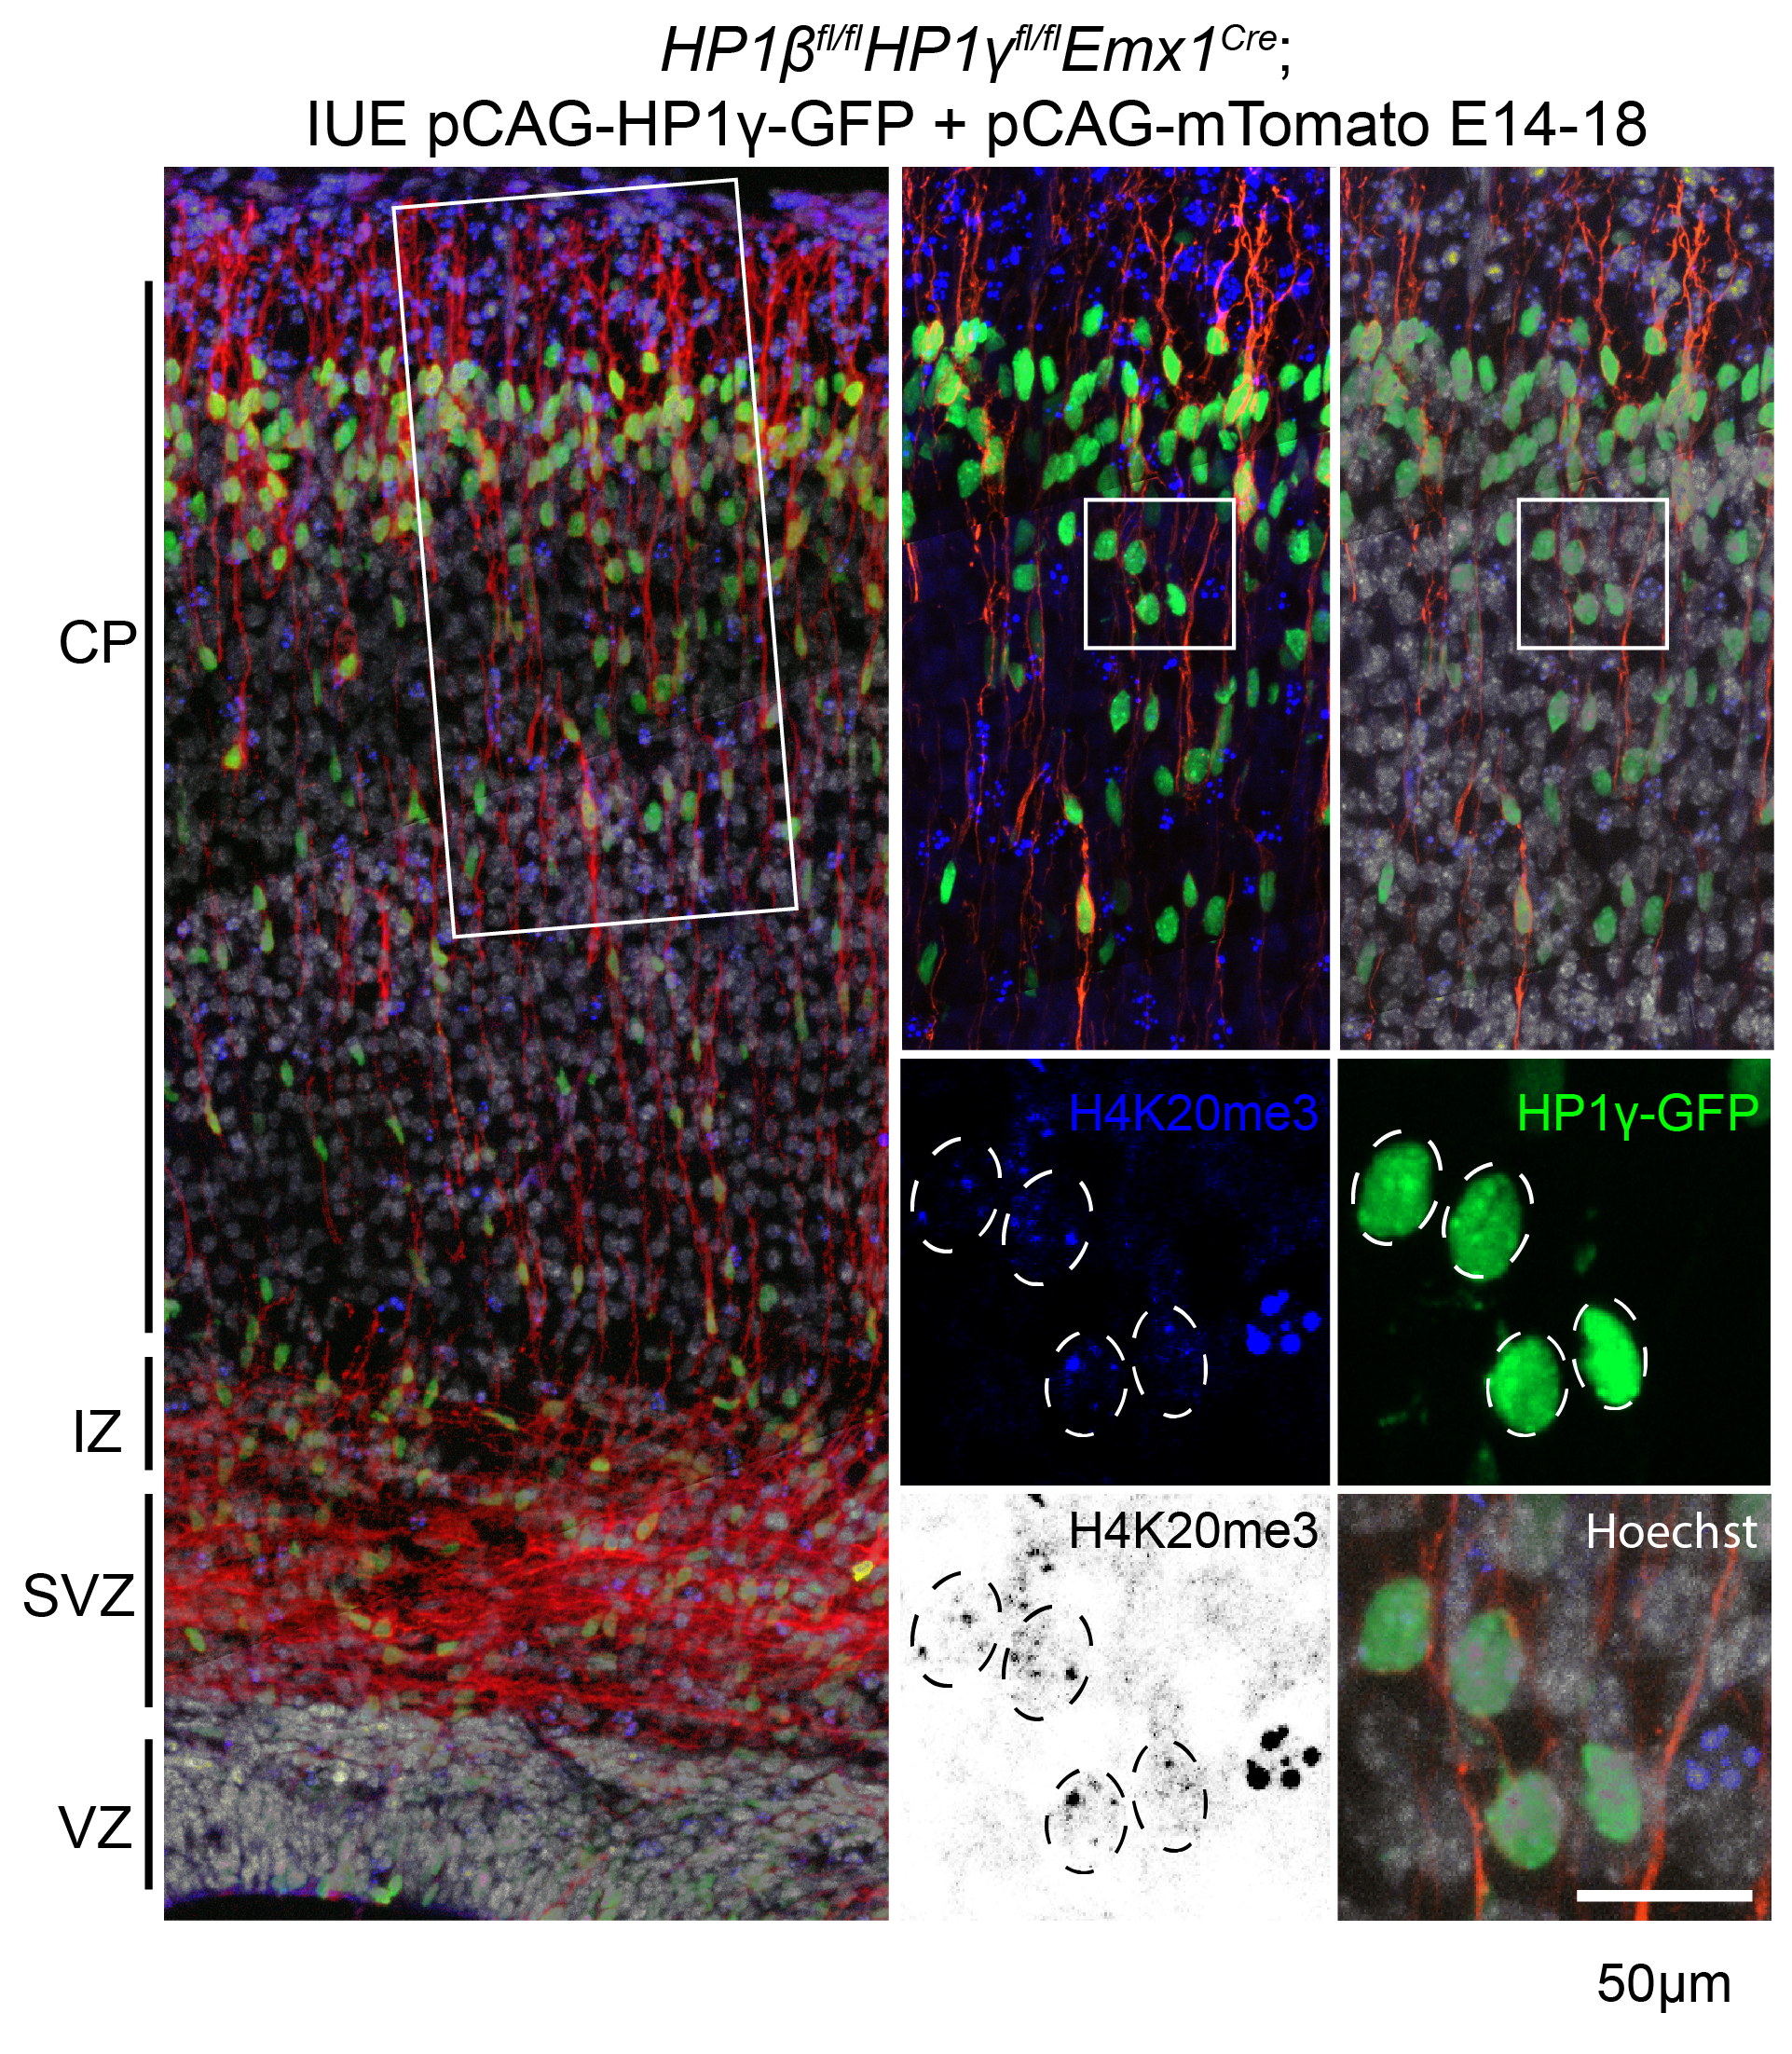
\includegraphics[width=1\linewidth, ]{./figure/results/H4K20me3rescue} 
  
  }
  
  \caption[Re-introduction of HP1$\gamma$ can restore H4K20me3]{Re-introduction of HP1$\gamma$ can restore H4K20me3.  Following Emx1-mediated deletion of HP1$\beta$ and HP1$\gamma$ at E10.5, re-introduction of HP1$\gamma$-GFP by in utero electroporation (IUE) at E14 restores H4K20me3 (magnification, white circles).}\label{fig:H4K20me3rescue}
  \end{figure}
  
  \subsection{H4K20me3 Loss is Correlated with IAP
  De-repression}\label{h4k20me3-loss-is-correlated-with-iap-de-repression}
  
  Given H4K20me3 is known to be important in silencing repeats, it
  followed that we could observe an exact correlation with loss of
  H4K20me3 and the de-repression of IAP elements there. Specifically, we
  observe that H4K20me3 is highly enriched in post-mitotic neurons of the
  cortex and hippocampus, which is also where we observe IAP de-repression
  in the HP1\(\beta\)/\(\gamma\) DKO (Figure \ref{fig:H4K20me3corr}).
  
  \begin{figure}
  
  {\centering 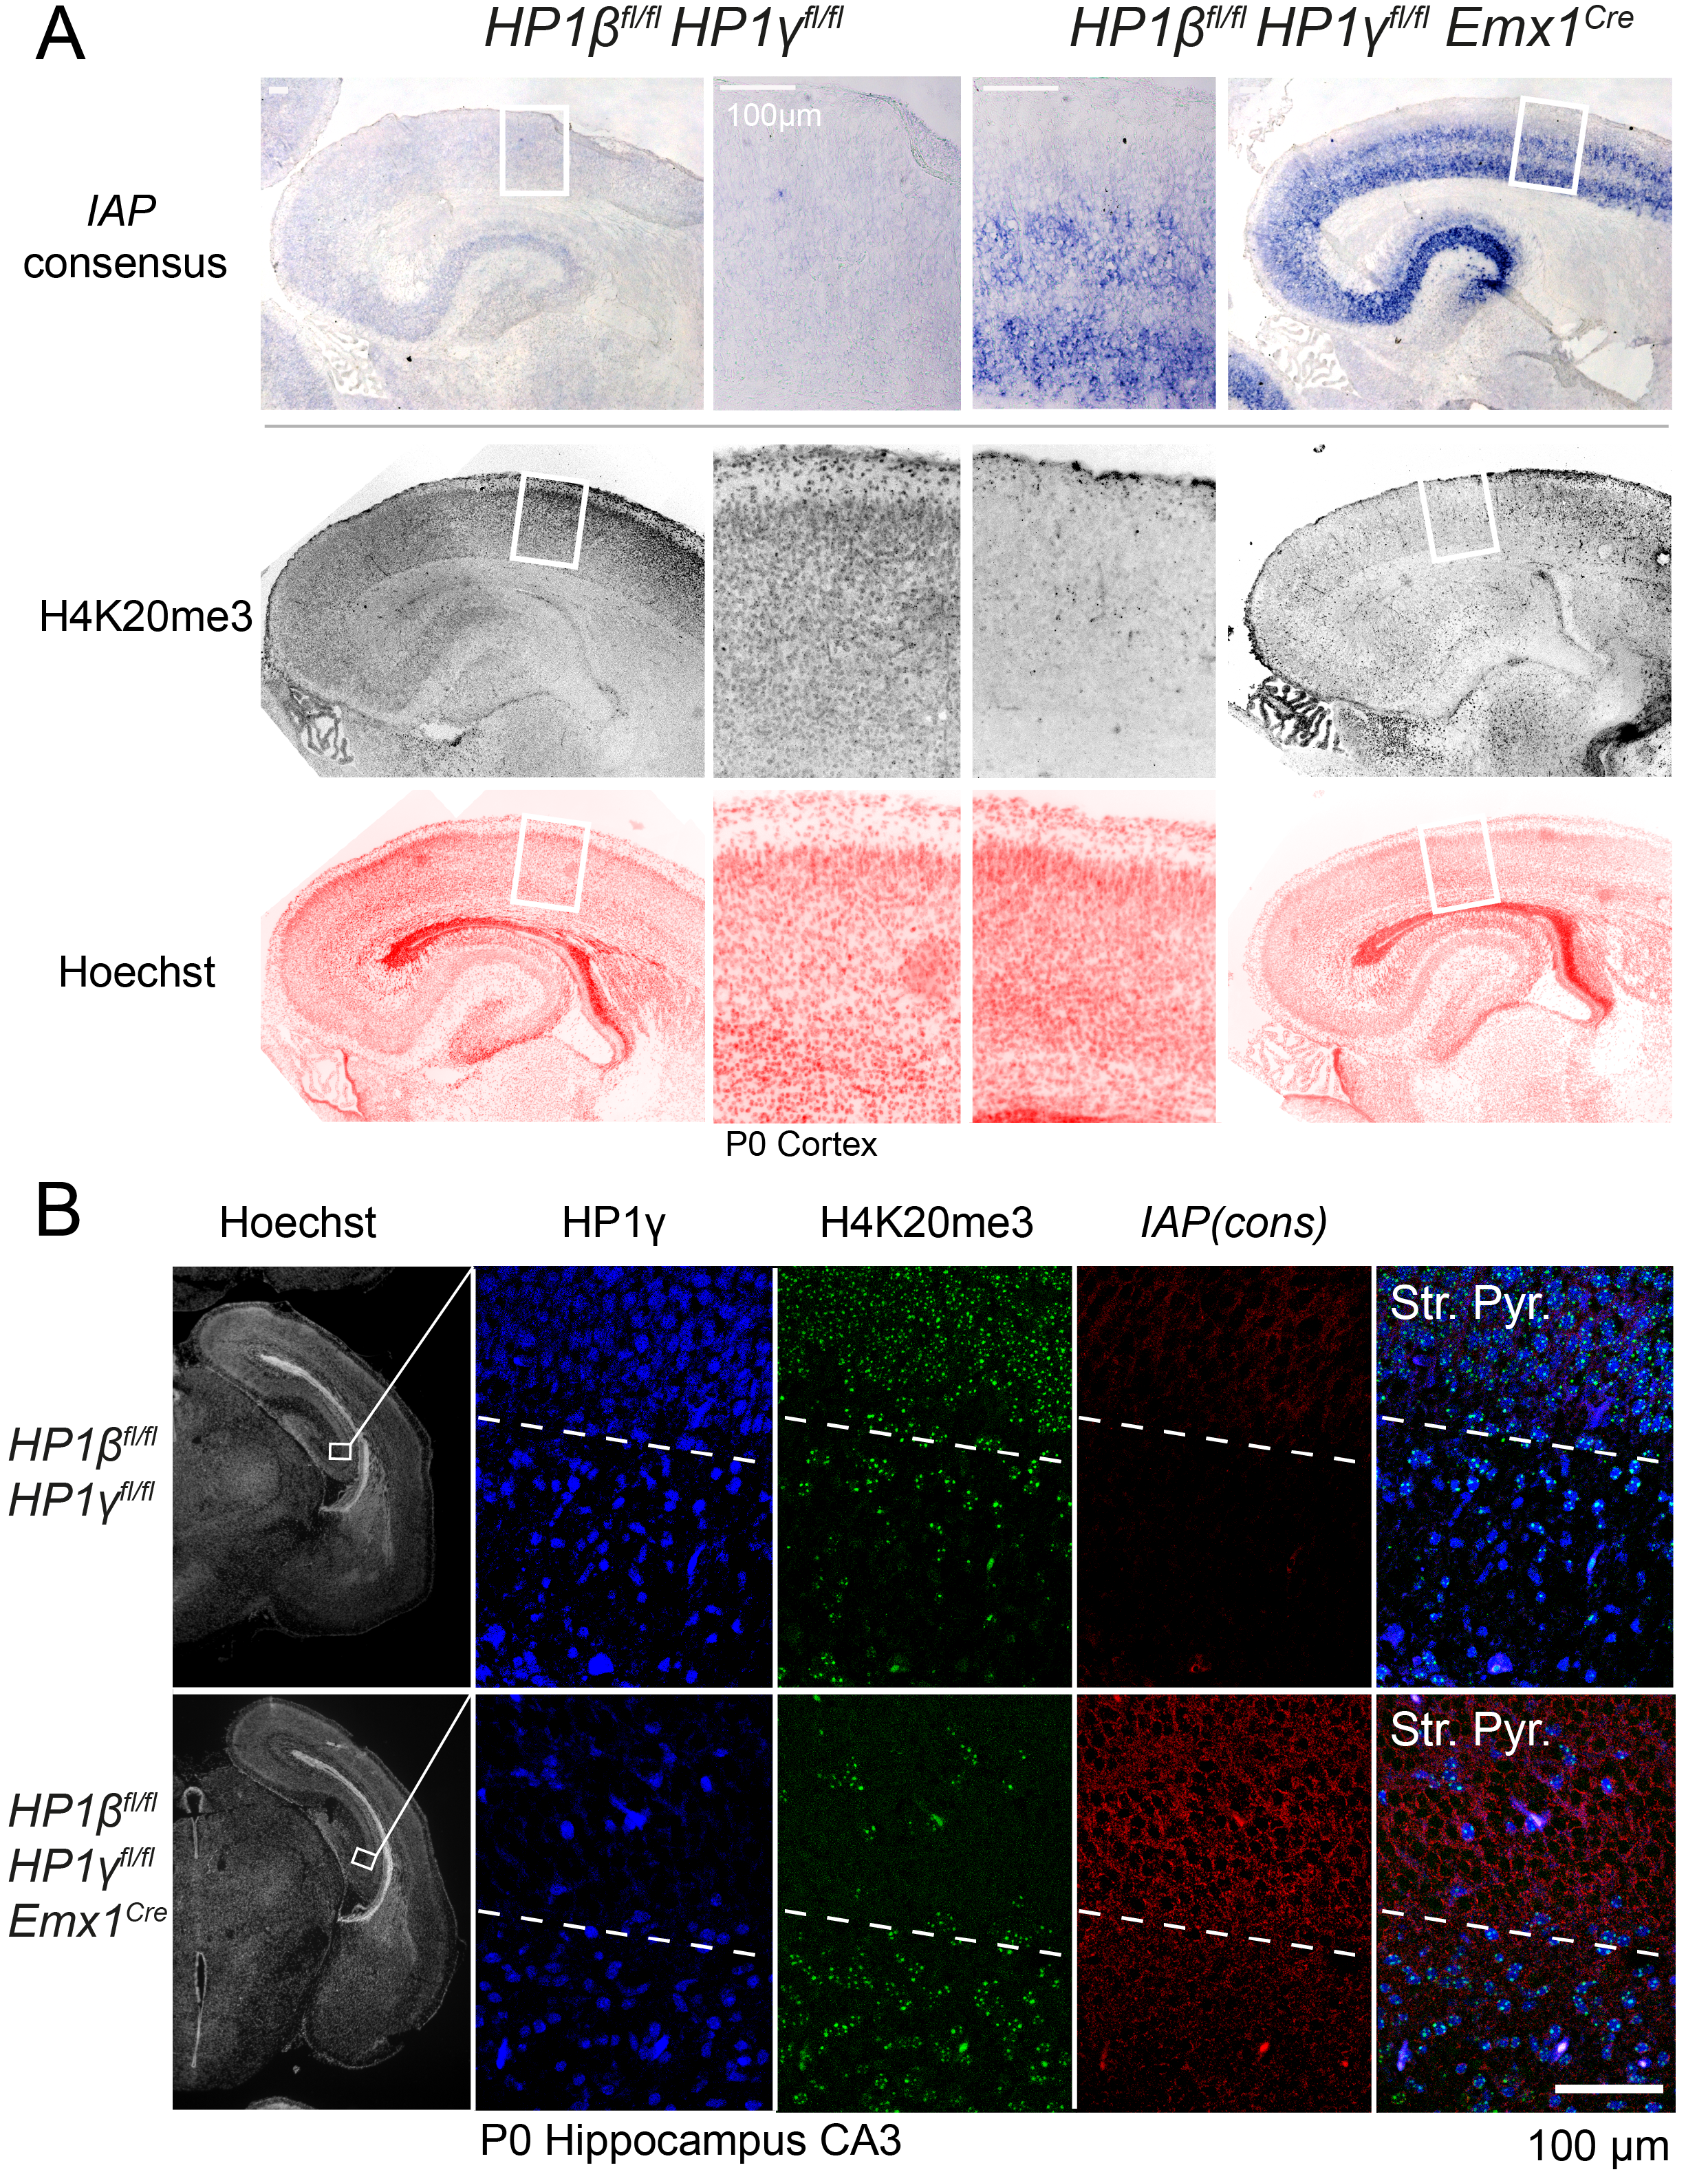
\includegraphics[width=0.85\linewidth, ]{./figure/results/H4K20me3_4} 
  
  }
  
  \caption[H4K20me3 loss is Correlated with IAP De-Repression]{H4K20me3 loss is Correlated with IAP De-Repression. (A) In situ hybridization using the IAP consensus probe on P0 sections followed by IHC for H4K20me3 and DAPI on the next serial section with magnification on the cortex. (B) Combined fluorescent ISH/IHC of IAP and H4K20me3 and HP1$\gamma$ in the developing CA3 field.  Robust IAP signal can be observed in the stratum pyramidale (Str. Pyr.) where HP1$\gamma$ and H4K20me3 are lost in post-mitotic CA3 neurons.}\label{fig:H4K20me3corr}
  \end{figure}
  
  \FloatBarrier
  
  However, as evidenced by ISH (Figure \ref{fig:IAPcons}) and RNAseq from
  HP1\(\gamma\) deficient neurons (Figure \ref{fig:RNAsum}), loss of
  H4K20me3 alone is not sufficient to induce de-repression of ERVK
  elements such as IAPs. Clearly, HP1\(\beta\) contributes an additional
  mechanism to the repression of these elements.
  
  \subsection{KAP1, H3K9me3 and H4K20me3 are lost at IAP Elements in
  HP1cTKO ES
  Cells}\label{kap1-h3k9me3-and-h4k20me3-are-lost-at-iap-elements-in-hp1ctko-es-cells}
  
  \begin{figure}
  
  {\centering \includegraphics[width=1\linewidth, ]{./figure/results/IAPEz-int_h3k9me3_H4K20me3} 
  
  }
  
  \caption[KAP1, H3K9me3 and H4K20me3 are Reduced at IAP Elements in HP1cTKO ES Cells]{KAP1, H3K9me3 and H4K20me3 are Reduced at IAP Elements in HP1cTKO ES Cells. (Top): Read coverage profiles of KAP1, H3K9me3 and H4K20me3 ChIP signals split by cluster. (Below): Heatmaps of raw ChIPseq signal (RPKM) over annotated IAPEz internal (-int) fragments, grouped by 3 kmeans clusters.}\label{fig:IAPH3K9}
  \end{figure}
  
  \FloatBarrier
  
  A collaboration with Dr.~Jafar Sharif (RIKEN, Yokohama, Japan) enabled
  interrogation into the effects of the loss of HP1 proteins in a single
  cell population. HP1cTKO ES cells are transgenic ES cells where all
  three HP1's (\(\alpha\), \(\beta\), \(\gamma\)) are floxed and can be
  excised following activation of an ERT2-Cre transgene. In these cells,
  following the addition of tamoxifen, Cre translocates to the nucleus and
  excises the targeted alleles, resulting in triple deletion of HP1
  proteins. Following 6 days of culture in the presence of tamoxifen, HP1
  proteins were verified to be deleted from these cells. Here we were able
  to observe the effect of complete loss of HP1 proteins on DNA
  methylation as well as any changes in the distribution of H3K9me3,
  H4K20me3 and KAP1.
  
  In addition to a large number of changes in gene transcription (data not
  shown), HP1cTKO ES cells show a de-repression of several ERVs, including
  IAPs, similar to that seen in HP1\(\beta\)/\(\gamma\) DKOs. ChIP-seq
  signal of KAP1, H3K9me3, and H4K20me3 was noticeably reduced from IAP
  elements (figure \ref{fig:IAPH3K9}). Consistent with the brain data,
  H4K20me3 appears to be completely lost, owing to deletion of
  HP1\(\gamma\). Noticeably, H3K9me3 and KAP1 are also reduced at IAP
  elements in HP1cTKO cells, implicating HP1 proteins to be necessary for
  assembly of the KAP1/SETDB1/SUV39H1 repressive complex at these repeats.
  
  \subsection{DNA Methylation is affected Following loss of
  HP1}\label{dna-methylation-is-affected-following-loss-of-hp1}
  
  \subsubsection*{\texorpdfstring{\emph{Non-Cannonically Imprinted Genes
  are Upregulated in HP1DKO
  Hippocampi}}{Non-Cannonically Imprinted Genes are Upregulated in HP1DKO Hippocampi}}\label{non-cannonically-imprinted-genes-are-upregulated-in-hp1dko-hippocampi}
  \addcontentsline{toc}{subsubsection}{\emph{Non-Cannonically Imprinted
  Genes are Upregulated in HP1DKO Hippocampi}}
  
  While transcriptional changes to a subset of canonically imprinted genes
  could not be detected by in situ hybridization (section \ref{imprint}),
  the neuronally expressed Neuronatin ( \emph{Nnat} ) and other
  non-canonically imprinted genes such as \emph{Xlr3a} and \emph{Xlr3c}
  are dysregulated in the HP1\(\beta\)/\(\gamma\) DKO and aged
  HP1\(\beta\)KO (clusters 4 \& 5, Figure \ref{fig:RNAsum}), and are
  summarized in table \ref{tab:imprintedtable}. While the majority of such
  genes are changed in DKO animals, Neuronatin shows de-repression in aged
  HP1\(\beta\) KO, suggesting that this may be due to a deficiency in
  DNMT1 maintaining the methylation imprint over a lifespan without
  HP1\(\beta\).
  
  \begin{table}[!h]
  
  \caption{\label{tab:imprintedtable}Imprinted Loci showing Elevated Transcription in HP1DKO Hippocampi}
  \centering
  \resizebox{\linewidth}{!}{
  \begin{tabular}{lllrrrr}
  \toprule
  Gene & Class & Chromosome & LogFC & logCPM & Pvalue & FDR\\
  \midrule
  Xlr3a & protein\_coding & X & 5.778093 & 1.2524118 & 0.0001989 & 0.0272010\\
  Xlr3c & protein\_coding & X & 8.440795 & 1.7659862 & 0.0000003 & 0.0002928\\
  Gm364 & protein\_coding & X & 6.553524 & 0.5700350 & 0.0000035 & 0.0018841\\
  Mkrn3 & protein\_coding & 7 & 3.510904 & 2.4471193 & 0.0000000 & 0.0000146\\
  Tsga8 & protein\_coding & X & 5.900168 & 0.3040211 & 0.0002019 & 0.0420649\\
  \addlinespace
  Uba1y & protein\_coding & Y & 4.554711 & 1.6450681 & 0.0000002 & 0.0002569\\
  Nnat & protein\_coding & 2 & 1.385290 & 7.4718652 & 0.0000006 & 0.0004993\\
  Mdga1 & protein\_coding & 17 & 1.176271 & 6.6211071 & 0.0001667 & 0.0357879\\
  \bottomrule
  \end{tabular}}
  \end{table}
  
  \subsubsection*{\texorpdfstring{\emph{HP1cTKO Cells Show Abberant DNA
  Methylation}}{HP1cTKO Cells Show Abberant DNA Methylation}}\label{hp1ctko-cells-show-abberant-dna-methylation}
  \addcontentsline{toc}{subsubsection}{\emph{HP1cTKO Cells Show Abberant
  DNA Methylation}}
  
  DNA methylation in HP1cTKO ES cells was measured by Reduced Read
  Bisulfite Sequencing (RRBSeq) (Figure \ref{fig:RRBScircos}). Following
  deletion of all HP1 proteins we could observe loss of DNA methylation at
  LINE and LTR repeats, and partial hypermethylation of promoters, exons
  and SINEs.
  
  \begin{figure}
  
  {\centering \includegraphics[width=1\linewidth, ]{./figure/results/HP1cTKO_RRBS} 
  
  }
  
  \caption[HP1cTKO ES Cells Show Abberant DNA Methylation]{HP1cTKO ES Cells Show Abberant DNA Methylation. (A) Scatterplot of methylation in HP1cTKO and WT cells. Hypermethylation of exons and promoters occurs, while intergenic regions become hypomethylated (B). A Circos plot (C) visualizes all changes occuring in the HP1cTKO RRBS data relative to WT by chromosome. The magnitude of change is represented on the radial y axis. The outermost ring represents methylation change density.  Inner rings annotate methylation changes occuring to CpG islands, exons, LTRs, LINEs and SINEs respectively.}\label{fig:RRBScircos}
  \end{figure}
  
  \subsection*{\texorpdfstring{\emph{KAP1 is lost from ICRs in HP1cTKO
  Cells}}{KAP1 is lost from ICRs in HP1cTKO Cells}}\label{kap1-is-lost-from-icrs-in-hp1ctko-cells}
  \addcontentsline{toc}{subsection}{\emph{KAP1 is lost from ICRs in
  HP1cTKO Cells}}
  
  To understand how imprinted loci may be affected in HP1cTKO ES cells, I
  examined Imprinting Control Regions (ICRs) that overlap with ZFP57
  binding (data from (Riso et al.
  \protect\hyperlink{ref-RisoZFP57maintainsparentoforiginspecific2016}{2016})).
  Figure \ref{fig:KAP1ICR}A shows the average binding of KAP1, H3K9me3 and
  H4K20me3 across these ICRs, centered at the ZFP57 peak. We observe a
  distinct loss of KAP1 at ICRs, one example of which is Neuronatin (
  \emph{Nnat} , Figure \ref{fig:KAP1ICR}B) where KAP1 binding near the CpG
  island is lost and RRBS shows a shift towards DNA hypermethylation at
  the CpG. Notably, like HP1\(\beta\)/\(\gamma\) DKO hippocampi,
  \emph{Nnat} expression is also elevated in HP1cTKO ES cells (Figure
  \ref{fig:KAP1ICR}B, bottom track). As methylation of the CpG would
  normally be associated with transcriptional repression, it is likely the
  signal observed here is the transcriptionally permissive
  5-hydroxymethylation (5hmC) modification, which cannot be distinguished
  from 5mC in bisulfite sequencing.
  
  \begin{figure}
  
  {\centering \includegraphics[width=0.75\linewidth, ]{./figure/results/KAP1_ICR_profile} 
  
  }
  
  \caption[KAP1 binding to Imprinting Control Regions is Lost in HP1cTKO ES Cells]{KAP1 binding to Imprinting Control Regions is Lost in HP1cTKO ES Cells. (A) KAP1 binding around ZFP57 peaks (Riso 2014) at 20 Imprinting Control Regions (ICRs) is lost in HP1cTKO ES cells. (B) Epigenetic Disorder at the Nnat ICR in HP1cTKO ES cells. RRBS track: Blue if methylation is 0-40\%, red if methylation is 60-100\%, and white if methylation is 40\%-60\%.}\label{fig:KAP1ICR}
  \end{figure}
  
  \FloatBarrier
  \clearpage
  
  \section{Transcriptional Dysregulation following HP1 Deficiency Drives
  UPR and Inflammatory Responses}\label{RNAresults}
  
  To gain insight into any transcriptional de-regulation occurring in HP1
  mutant hippocampi, 32bp paired-end total RNAseq was performed to detect
  any changes in both coding and non-coding RNA, including repetitive
  elements.
  
  \subsection{Genotype Related Changes}\label{genotype-related-changes}
  
  \subsubsection*{\texorpdfstring{\emph{Differential Gene
  Expression}}{Differential Gene Expression}}\label{differential-gene-expression}
  \addcontentsline{toc}{subsubsection}{\emph{Differential Gene
  Expression}}
  
  Surprisingly, relatively few genes were significantly changed in HP1
  mutant hippocampi. In examining such changes both a coarse analysis
  (Benjamin-Hochberg FDR \textless{} 0.05) and a stringent analysis (FDR
  \textless{} 0.01) was undertaken. To understand the primary effects the
  stringent analysis will first be discussed, followed by pathway analysis
  using the coarse analysis.
  
  Testing for significant changes between genotypes in the aged timepoint
  yields the heatmap seen in Figure \ref{fig:RNAsum}A where data from
  young animals is included (Figure \ref{fig:RNAsum}B. Notably, testing
  within batch for differential gene expression between WT and DKO
  genotypes in young animals largely gives the same gene set (data not
  shown), suggesting transcriptional differences are minimal between the 3
  month DKO and the 13 month DKO.
  
  Hierarchical clustering of differentially expressed genes reveals
  distinct sets associated with genotype (Figure \ref{fig:RNAsum}B).
  Clusters 1 \& 2 include genes that are underrepresented compared to WT.
  It is clear that cluster 1, which shows underrepresentation in
  HP1\(\beta\)KO and HP1DKO, comprises genes associated with the dentate
  gyrus, so their underrepresentation is not due to altered expression,
  rather a complete lack of the tissue that normally expresses them.
  Cluster 2 comprises a handful of genes that are in the vicinity of the
  HP1\(\gamma\) gene locus, which infers their expression was affected due
  to local genomic changes following deletion of the HP1\(\gamma\) gene.
  
  Genes and repeats in clusters 3, 4 and 5 have elevated expression
  compared to wildtype, due to either singular loss of HP1\(\gamma\)
  (cluster 3), HP1\(\beta\) (cluster 4) or both (cluster 5). Strikingly,
  from cluster 3 we can observe that the primary effect due to loss of
  HP1\(\gamma\) is elevated transcription of the protocadherin cluster on
  chromosome 18, which will be discussed later. Cluster 4 contains genes
  which are elevated in aged HP1\(\beta\) animals and HP1DKO animals, one
  of which is the known imprinted gene Neuronatin ( \emph{Nnat} ).
  
  Cluster 5 contains protein coding genes, lncRNAs and repeats which show
  elevated transcription only in the HP1\(\beta\)/\(\gamma\) double mutant
  and will be discussed in the next section.
  
  \begin{figure}
  
  {\centering \includegraphics[width=1\linewidth, ]{./figure/results/RNA_summary} 
  
  }
  
  \caption[High Confidence Differential Gene Expression in HP1 Mutant Adult Hippocampi]{High Confidence Differential Gene Expression in HP1 Mutant Adult Hippocampi. Volcano plots (A) display log fold changes with respect to corrected p value (aged).  (B) Hierarchical clustering of differentially expressed genes (corrected p < 0.01)  across all samples.}\label{fig:RNAsum}
  \end{figure}
  
  \FloatBarrier
  \newpage
  
  \subsubsection*{\texorpdfstring{\emph{Read Coverage of
  lncRNAs}}{Read Coverage of lncRNAs}}\label{read-coverage-of-lncrnas}
  \addcontentsline{toc}{subsubsection}{\emph{Read Coverage of lncRNAs}}
  
  Given the statistically significant de-repression of several lncRNAs, I
  looked at lncRNA read coverage across the entire genome in each of the
  mutants (Figure \ref{fig:lncRNAcov}). Global de-repression of annotated
  long non-coding RNAs infers significant alterations to heterochromatin
  boundaries. Notably, transcription of lncRNAs increases steadily with
  age, in an effect that appears to be dependent on HP1\(\beta\).
  
  \begin{figure}
  
  {\centering \includegraphics[width=1\linewidth, ]{./figure/results/lncRNACov} 
  
  }
  
  \caption[LncRNA transcription is elevated in HP1 Mutants]{LncRNA Transcription is Elevated in HP1 Mutants.  Read coverage heatmaps of all lncRNAs genome-wide (bottom) plot all alignments per 50bp bin for each lncRNA locus including 1 kilobase upstream of the transcription start site (TSS) and 1 kilobase downstream of the transcription end site (TES), which are scaled to be the same size.  Read coverage profiles (top) profide an overview of genome-wide changes in lncRNA transcription.}\label{fig:lncRNAcov}
  \end{figure}
  
  \FloatBarrier
  
  \subsubsection*{\texorpdfstring{\emph{Read Coverage at Repeat
  Flanks}}{Read Coverage at Repeat Flanks}}\label{read-coverage-at-repeat-flanks}
  \addcontentsline{toc}{subsubsection}{\emph{Read Coverage at Repeat
  Flanks}}
  
  A similar analysis was undertaken for LINE, SINE and LTR repeat classes
  (Figure \ref{fig:readcov}). In the case of repeats, observing
  transcription at sequences that are upstream or downstream (ie sequences
  that `flank' the repeat) can be informative for cases where the repeat
  cannot be mapped. From (Figure \ref{fig:readcov}A), where the read
  coverage in repeat flanks is markedly higher than the internal repeat,
  we can assume that our measured counts of repeat transcripts are an
  underestimate of what is actually occurring \emph{in vivo}. Significant
  de-repression of repeat type plotted by class (Figure
  \ref{fig:readcov}B) reveals the most significant changes occur in the
  ERVK and ERV1 families.
  
  \begin{figure}
  
  {\centering \includegraphics[width=1\linewidth, ]{./figure/results/Repeatcovsig} 
  
  }
  
  \caption[Read Coverage at Repeat Flanks in HP1 Mutants and Significant Changes by Repeat Class]{Read Coverage at Repeat Flanks in HP1 Mutants and Significant Changes by Repeat Class. (A) Read coverage profiles and heatmaps of LINE, SINE and LTR repeat classes.  Repeats are scaled to be aligned by their 5' end and their 3' end in addition to 1kb upstream and downstream. (B) Significant changes in repeats by repeat familly.  The most significant changes in HP1DKO belong to ERVK and ERV1 families.}\label{fig:readcov}
  \end{figure}
  
  \FloatBarrier
  \clearpage
  
  \subsubsection*{\texorpdfstring{\emph{Chimeric
  Transcription}}{Chimeric Transcription}}\label{chimeric-transcription}
  \addcontentsline{toc}{subsubsection}{\emph{Chimeric Transcription}}
  
  Given the elevated transcription of ERV elements, I examined how this
  may contribute to chimeric transcription events-where transcription
  begins in a repeat-such as an LTR, and `reads into' a coding gene or
  exon. The resultant transcript is a `chimera' where it contains both the
  repeat and exon sequence. This may result in alternative splicing events
  or direct activation of entire genes. To find such transcripts I
  implemented a customized version of the LIONS pipeline (Babaian et al.
  \protect\hyperlink{ref-BabaianLIONSAnalysisSuite2018}{2018}) to run on
  the BIH CUBI cluster. A strong trend can be observed in LTR-derived
  chimeric transcripts in DKO animals (Figure \ref{fig:chimeras}), where
  increased transcription of the repeat correlates with increased
  transcription of the adjacent exon. While most chimeric events are
  small, pertaining to exon inclusion or retention, elevated transcription
  in a subset of genes in Cluster 5 is due to direct activation by an
  adjacent repeat (Table \ref{tab:chimeratable} \& Figure
  \ref{fig:chimeras}). \newline
  \newline
  
  \begin{table}[!h]
  
  \caption{\label{tab:chimeratable}Gene Expression Changes in HP1$\beta$/$\gamma$ DKO Hippocampi due to Chimeric Transcription Originating in an Adjacent Repeat}
  \centering
  \resizebox{\linewidth}{!}{
  \begin{tabular}{lllrrr}
  \toprule
  Name & Class & AdjacentRepeat & logFC & PValue & FDR\\
  \midrule
  Gm48619 & lncRNA & IAP & 6.809431 & 0.0000000 & 0.0000000\\
  Kank4os & antisense & RLTR31C\_MM & 8.334549 & 0.0000000 & 0.0000052\\
  Gm28321 & lncRNA & IAP & 9.281399 & 0.0000000 & 0.0000052\\
  Got1l1 & protein\_coding & multiple LTRs & 3.685565 & 0.0000002 & 0.0002764\\
  E230025N22Rik & protein\_coding & mixed & 3.852652 & 0.0000004 & 0.0003757\\
  \addlinespace
  Akr1c13 & protein\_coding & ERVB7? & 6.067095 & 0.0000005 & 0.0004745\\
  Gramd1c & protein\_coding & IAP & 1.901830 & 0.0000042 & 0.0021810\\
  G730013B05Rik & lncRNA & RLTR31B2 & 6.867196 & 0.0000046 & 0.0022764\\
  Olfr316 & protein\_coding & RLTR44C & 2.337525 & 0.0000083 & 0.0038010\\
  Gm15398 & lncRNA & MTA\_mm & 6.430798 & 0.0000148 & 0.0063698\\
  \addlinespace
  Serpinb1c & protein\_coding & IAP & 7.012703 & 0.0000343 & 0.0116408\\
  Smarca5-ps & processed\_pseudogene & IAPEY3-int & 6.451726 & 0.0000365 & 0.0120489\\
  Cyp2b13 & protein\_coding & IAP & 7.271137 & 0.0000601 & 0.0125165\\
  Mnd1 & protein\_coding & IAP & 5.634051 & 0.0000676 & 0.0189726\\
  Umodl1 & protein\_coding & RLTR17B\_Mm & 2.841678 & 0.0001121 & 0.0274364\\
  \addlinespace
  Gsta2 & protein\_coding & MT2B & 5.357106 & 0.0001169 & 0.0190674\\
  Patj & protein\_coding & IAP & 1.513902 & 0.0001566 & 0.0346798\\
  Dmp1 & protein\_coding & RMER19B and IAPLTR2b & 1.824824 & 0.0001642 & 0.0243289\\
  Btnl7-ps & unprocessed\_pseudogene & IAP1-MM\_I-int & 4.094741 & 0.0001794 & 0.0255045\\
  Gm13110 & lncRNA & MTEa & 1.889639 & 0.0001809 & 0.0255511\\
  \addlinespace
  Platr25 & protein\_coding & mixed & 1.979744 & 0.0004374 & 0.0457926\\
  \bottomrule
  \end{tabular}}
  \end{table}
  
  \FloatBarrier
  
  \begin{figure}
  
  {\centering \includegraphics[width=1\linewidth, ]{./figure/results/Hexplot_thesis2} 
  
  }
  
  \caption[Chimeric Transcription Events in HP1 Mutant Hippocampi]{Chimeric Transcription Events in HP1 Mutant Hippocampi.  (A) Co-transcription plots, where each point represents a chimeric transcript. Hexplots were used to correct for overplotting at low RPKM.  As can be observed in LTR-derived chimeras in aged HP1DKO animals (yellow square), higher transcription of the repeat (Reads Per Kilobase per Million reads (RPKM)), results in higher transcription of the exon portion of the chimera.  Black axes in each plot represent the mean Exon-RPKM (horizontal line) and the mean Repeat-RPKM (vertical line) in chimeras observed in wild-type of that repeat class and age. (B) An example chimeric transcript. An IAP element inside the first intron of Mnd1 results in transcriptional activation of the entire gene.}\label{fig:chimeras}
  \end{figure}
  
  \FloatBarrier
  
  \subsection{Longitudinal Changes To Gene
  Expression}\label{longitudinal-changes-to-gene-expression}
  
  Following initial data exploration, a non-negligible batch effect (see
  methods \ref{tab:colData}) dictated that it was unfavorable to conduct
  direct longitudinal comparisons of WT and DKO (Young WT vs Aged WT and
  Young DKO vs Aged DKO). However, testing for differential expression in
  HP1\(\beta\) and HP1\(\gamma\) single mutants across age (within batch)
  yielded minimal results. For HP1\(\gamma\)KO for instance, no
  differential expression passes an FDR \textless{} 0.01 or 0.05. For
  age-related changes in HP1\(\beta\)KO, no genes pass an FDR \textless{}
  0.01, and only a small number (184 genes) pass FDR \textless{} 0.05. The
  top ten upregulated genes by ascending p value are presented in Table
  \ref{tab:BKOtop}, with C4b being a notable top hit. The complete gene
  list of age-related expression changes in HP1\(\beta\)KO hippocampi is
  found in supplementary data \ref{DE}.
  
  \begin{table}[t]
  
  \caption{\label{tab:BKOtop}Top 10 Upregulated Genes due to Age in HP1$\beta$KO}
  \centering
  \resizebox{\linewidth}{!}{
  \begin{tabular}{llrrrrr}
  \toprule
  Gene & Gene.Biotype & logFC & logCPM & F & p.Value & FDR\\
  \midrule
  C4b & protein coding & 1.968703 & 6.167731 & 40.90800 & 6.00e-07 & 0.0120851\\
  Aldh16a1 & protein coding & 3.383482 & 2.733340 & 35.91748 & 1.70e-06 & 0.0132210\\
  Rprm & protein coding & 1.742288 & 4.544562 & 33.25780 & 3.20e-06 & 0.0132210\\
  Ethe1 & protein coding & 2.724653 & 2.706537 & 32.55687 & 3.80e-06 & 0.0132210\\
  Dmap1 & protein coding & 1.433555 & 4.434852 & 32.53388 & 3.80e-06 & 0.0132210\\
  \addlinespace
  Gm26917 & lincRNA & 2.189478 & 5.305955 & 31.10771 & 5.30e-06 & 0.0160351\\
  Caly & protein coding & 1.699563 & 6.281637 & 29.16404 & 8.70e-06 & 0.0213195\\
  Gstm4 & protein coding & 2.351643 & 3.047190 & 28.51131 & 1.03e-05 & 0.0216079\\
  Alad & protein coding & 1.680305 & 3.891168 & 27.85071 & 1.22e-05 & 0.0233221\\
  Podxl2 & protein coding & 1.496893 & 6.484461 & 27.43499 & 1.36e-05 & 0.0238435\\
  \bottomrule
  \end{tabular}}
  \end{table}
  
  \subsection{Pathway Analysis}\label{pathway-analysis}
  
  \subsubsection*{\texorpdfstring{\emph{Innate Immune Pathways are
  Activated from Prolonged Absence of
  HP1\(\beta\)KO}}{Innate Immune Pathways are Activated from Prolonged Absence of HP1\textbackslash{}betaKO}}\label{innate-immune-pathways-are-activated-from-prolonged-absence-of-hp1betako}
  \addcontentsline{toc}{subsubsection}{\emph{Innate Immune Pathways are
  Activated from Prolonged Absence of HP1\(\beta\)KO}}
  
  In accordance with the changes observed in HP1\(\beta\)/\(\gamma\) DKO
  hippocampi, the majority of the changes that occur due to sustained
  absence of HP1\(\beta\)KO occurs in the realm of upregulation. Of the
  184 genes differentially expressed in aged HP1\(\beta\)KO hippocampi
  compared to their youthful counterparts, 43 genes (24\%) are
  downregulated, such as Prox1 and others that may suggest a progressive
  loss of the dentate gyrus. The majority of changes lies in 141 genes
  (76\%) which are upregulated. Upon testing for age-related changes to
  gene transcription in HP1\(\beta\)KO hippocampi, aged HP1\(\beta\)KO
  cluster strongly with HP1\(\beta\)/\(\gamma\) DKO samples (Figure
  \ref{fig:BKOreactome}, left). Following a reactome pathway analysis
  (\url{https://reactome.org}, Fabregat et al.
  (\protect\hyperlink{ref-FabregatReactomePathwayKnowledgebase2018}{2018}))
  it became clear that the sustained absence of HP1\(\beta\) results in
  cellular stress and immune responses akin to viral infection (Figure
  \ref{fig:BKOreactome}, right).
  
  \begin{figure}
  
  {\centering \includegraphics[width=1\linewidth, ]{./figure/results/BKO_long_reactome} 
  
  }
  
  \caption[Pathway Analysis of Longitudinal Changes in HP1$\beta$KO]{Pathway Analysis of Longitudinal Changes in HP1$\beta$KO. (Left): Volcano plot and hierachical clustering following testing between aged HP1$\beta$KO and young HP1$\beta$KO. (Right): Top 25 reactome pathways from genes upregulated in aged HP1$\beta$KO.}\label{fig:BKOreactome}
  \end{figure}
  
  \subsubsection*{\texorpdfstring{\emph{UPR and Innate Immune Pathways are
  Activated in HP1\(\beta\)/\(\gamma\)
  DKO}}{UPR and Innate Immune Pathways are Activated in HP1\textbackslash{}beta/\textbackslash{}gamma DKO}}\label{upr-and-innate-immune-pathways-are-activated-in-hp1betagamma-dko}
  \addcontentsline{toc}{subsubsection}{\emph{UPR and Innate Immune
  Pathways are Activated in HP1\(\beta\)/\(\gamma\) DKO}}
  
  \begin{figure}
  
  {\centering \includegraphics[width=1\linewidth, ]{./figure/results/reactome_out} 
  
  }
  
  \caption[Analysis of Pathways Upregulated in HP1$\beta$/$\gamma$ DKO Hippocampi]{Analysis of Pathways Upregulated in HP1$\beta$/$\gamma$ DKO Hippocampi.  (Left): Volcano plot and hierachical clustering following testing between all HP1$\beta$/$\gamma$ DKO (young and aged) and all WT (young and aged).  (Right): Top 25 rectome pathways from genes upregulated in HP1$\beta$/$\gamma$ DKO across ages.}\label{fig:reactome}
  \end{figure}
  
  To examine the cellular response to loss of HP1\(\beta\) and
  HP1\(\gamma\) and the de-repression of non-coding regions, the
  up-regulated gene set from the `coarse' analysis (FDR \textless{} 0.05)
  was analysed on reactome (Figure \ref{fig:reactome}). Hierarchical
  clustering of the coarse set reveals that transcriptomic signatures of
  HP1\(\gamma\)KO hippocampi to be most similar to WT, excepting
  dysregulation of the protocadherin cluster (Figure \ref{fig:reactome},
  left). In HP1\(\beta\)/\(\gamma\) DKO hippocampi, upregulated pathways
  comprise the unfolded protein response, innate immune responses
  including complement activation, neuromodulatory pathways such as
  dopamine and serotonin release, amongst other pathways important for
  synaptic function. It should be noted that protocadherins (Pcdhs) do not
  contribute to neurotransmitter pathway over-representation, as they are
  not presently annotated in reactome.org.
  
  If one compares genes differentially expressed in aged HP1\(\beta\)KO
  with those changed in HP1\(\beta\)/\(\gamma\) DKO, a small subset of
  genes overlap which include complement components \emph{C4b} and
  \emph{C1qa} (Figure \ref{fig:C4}A). While \emph{Nnat} is highly
  significant in the HP1DKO dataset, it narrowly fails FDR in the young vs
  aged HP1\(\beta\)KO test statistic. C4 protein can be observed in CA3
  cell bodies as well as GFAP-positive astrocytes in Aged HP1\(\beta\)KO
  and HP1\(\beta\)/\(\gamma\) DKO hippocampi (Figure \ref{fig:C4}B).
  
  \begin{figure}
  
  {\centering \includegraphics[width=1\linewidth, ]{./figure/results/C4_GFAP} 
  
  }
  
  \caption[HP1$\beta$ Deficiency Results in Elevated C4 Expression in CA3 Pyramidal Neurons]{(A) Intersection of Differential expression in HP1$\beta$/$\gamma$ DKO and Aged HP1$\beta$KO. (B) HP1$\beta$ Deficiency results in Elevated C4 Expression in CA3 Pyramidal Neurons}\label{fig:C4}
  \end{figure}
  
  The age-dependent upregulation of ncRNAs, repeats and ERVs in
  HP1\(\beta\)KO, coincides with pathway analysis that suggests an
  anti-viral response (Figure \ref{fig:BKOreactome}) is instigated
  following prolonged de-repression of endogenous retroviruses in the
  hippocampus. As ERV de-repression is even more robust in HP1DKO
  hippocampi, the 689 transcripts differentially regulated in HP1DKO were
  cross checked against the interferome database
  (\url{http://www.interferome.org}), where \textasciitilde{}15\% (88/565
  protein coding genes) were found to overlap with cellular responses to
  interferons. Notably, the majority of the overlap (55) occurred from a
  previously published experiment where cortical neurons were treated with
  Interferon \(\beta\) ( \emph{IFN\(\beta\)} ) and their transcriptome
  analysed. The immune response occurring in HP1\(\beta\)/\(\gamma\) DKO
  neurons involves upregulation of innate immunity related \emph{Oas3},
  \emph{Lyk6}, \emph{Wdfy4}, \emph{Zap70}, \emph{Ly6e}, \emph{Ctsz},
  \emph{Il34}, \emph{Reep6}, \emph{Crlf2}, complement \emph{C3},
  \emph{C4b}, \emph{C1qa}, apoptosis-related \emph{Hrk} and \emph{Aatk},
  interferon response genes \emph{Ifitm2}, \emph{Ifi27}, and the
  regulatory component of the Interferon gamma receptor, \emph{Ifngr2}.
  The complete list of genes overlapping with the interferome is found in
  supplementary table \ref{tab:bkotable}.
  
  \begin{figure}
  
  {\centering 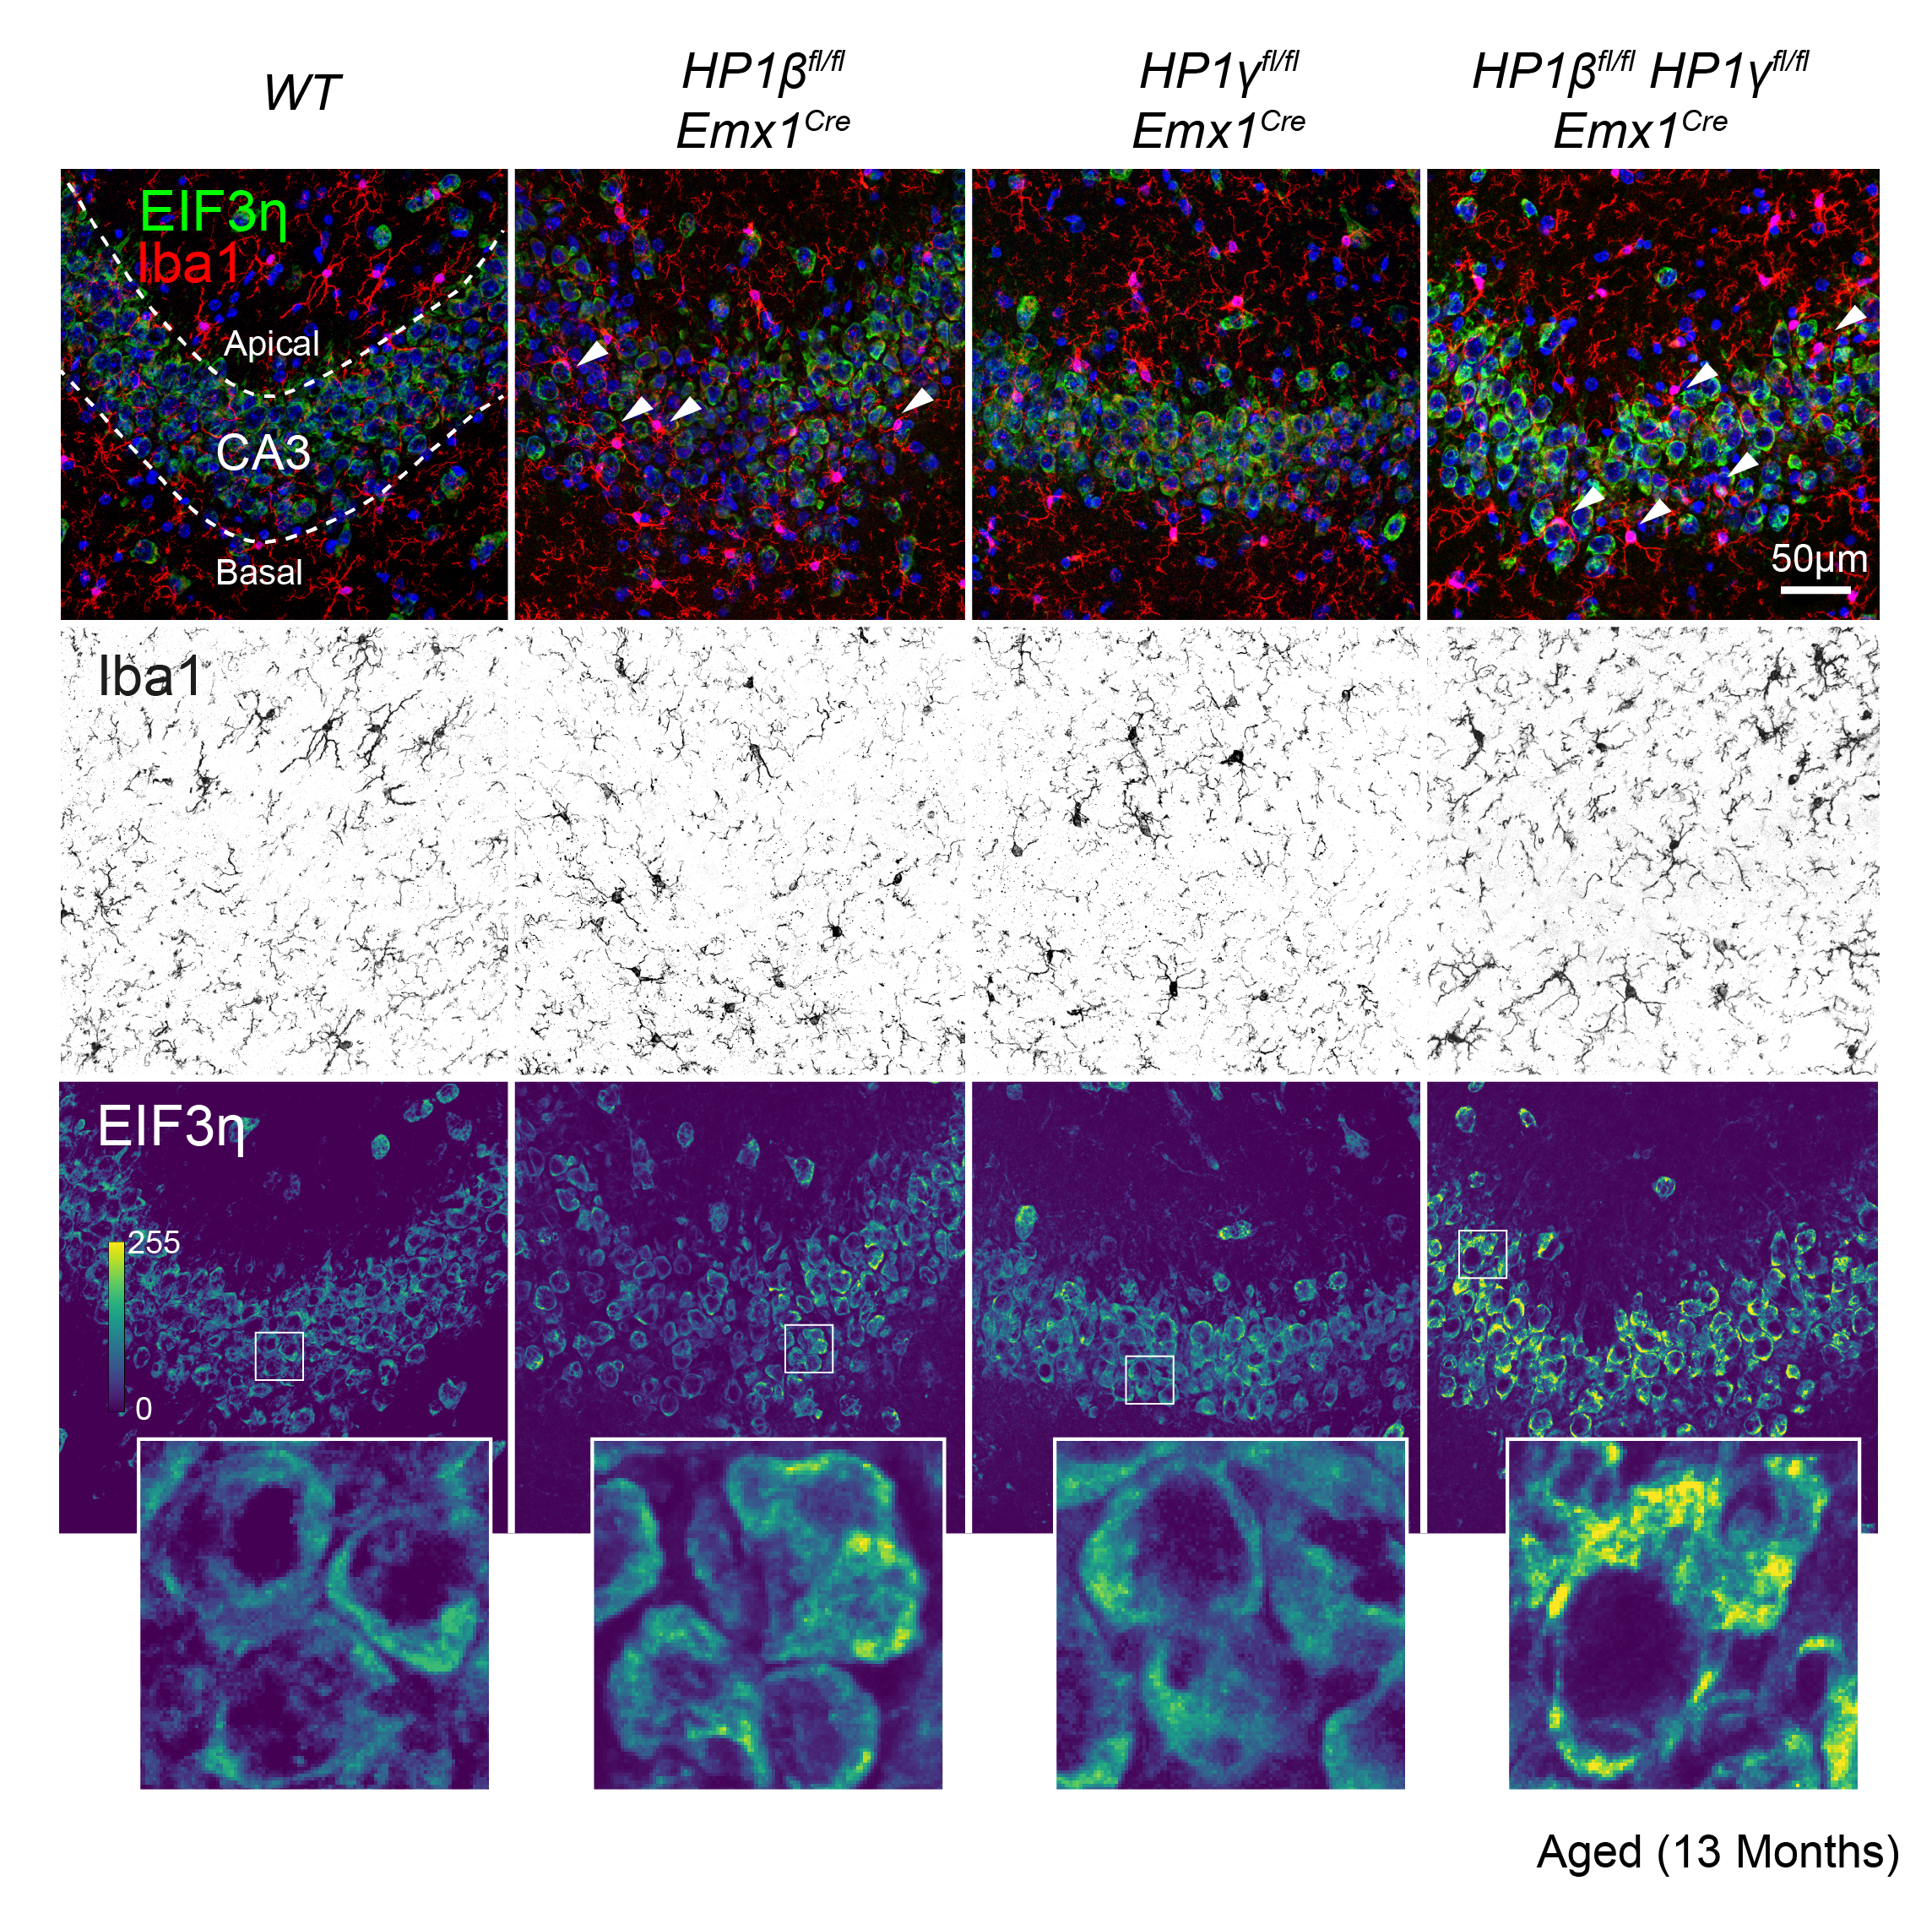
\includegraphics[width=1\linewidth, ]{./figure/results/EIF3} 
  
  }
  
  \caption[HP1$\beta$/$\gamma$ DKO Hippocampi show Evidence of Stress Granules and increased Infiltration of Microglia]{HP1$\beta$/$\gamma$ DKO Hippocampi show Evidence of Stress Granules and increaseed Infiltration of Microglia. IHC of Aged CA3 fields using Hoechst (nuclei, Blue) EIF3$\eta$ (stress granules, green) and Iba1 (microglia, red).  HP1$\beta$KO and HP1$\beta$/$\gamma$ DKO show increased invasion of microglia (white arrows) into the Stratum pyramidale. The third row shows a single channel of EIF3$\eta$ staining intensity coded to the viridis colour palette on the 0-255 colour scale.}\label{fig:EIF3}
  \end{figure}
  
  Additionally, multiple genes normally attributed to chemotaxis/invasion
  ( \emph{Mmp14}, \emph{Mmp17}, \emph{Mpped1}, \emph{Adam11}, \emph{Cck})
  and phagocytosis ( \emph{Cd302} and the synapse-specific \emph{C1ql2})
  were differentially affected. This suggested that the end result of the
  inflammatory cascade could be resulting in the activation of microglia.
  Recent work has elucidated a role for microglia in synaptic pruning
  which appears to rely on complement proteins in the CNS (Stevens et al.
  \protect\hyperlink{ref-StevensClassicalComplementCascade2007}{2007}),
  and dysregulation of complement proteins is now understood to underlie a
  wide range of inflammatory diseases in the CNS including
  neurodegeneration (Bodea et al.
  \protect\hyperlink{ref-BodeaNeurodegenerationActivationMicroglial2014}{2014}),
  Multiple sclerosis (Christensen et al.
  \protect\hyperlink{ref-ChristensenGeneenvironmentinteractions2007a}{2007}),
  Alzheimer's' (Fischer et al.
  \protect\hyperlink{ref-FischerComplementC1qC31995}{1995}), ALS (Lee et
  al. \protect\hyperlink{ref-LeeComplementcomponentsare2018}{2018}), and
  normal aging (Stephan et al.
  \protect\hyperlink{ref-StephanDramaticIncreaseC1q2013}{2013}). The
  sustained elevated transcription of \emph{C3}, \emph{C4} and \emph{C1qa}
  in HP1\(\beta\)KO and HP1\(\beta\)/\(\gamma\) DKO hippocampi is likely
  to result in increased infiltration and phagocytosis of neuronal
  synapses by microglia. This can be summarily seen in figure
  \ref{fig:EIF3}, where increased transcription of lncRNA and
  retroelements due to loss of HP1\(\beta\) and HP1\(\gamma\) has resulted
  in innate immune and unfolded protein responses. In the \emph{Stratum
  pyramidale} where the CA3 cell bodies reside, an innate immune response
  has induced invasion of microglia while condensation of EIF3\(\eta\)+
  stress granules is visible in CA3 cell bodies, indicative of UPR
  activation there.
  
  All of the players in the aforementioned pathway have known links to
  inflammatory disease states, neurodegeneration, and normal aging. The
  potential causes of these cascades, along with their relevance to human
  aging and disease, will be examined in the next section.
  
  \chapter{Discussion}\label{discussion}
  
  Given that epigenetic drift occurs over the course of normal aging, the
  effect of deletion of two non-histone proteins HP1\(\beta\) and
  HP1\(\gamma\) was examined to determine if heterochromatin loss is
  causal in the intrinsic aging of the mammalian brain.
  \emph{Emx1}-mediated deletion of HPI\(\beta\) impairs neurogenesis
  resulting in malformation of the infrapyramidal blade of the dentate
  gyrus and a subsequent progressive reduction in the complexity of CA3
  basal dendrites. This malformation of the dentate gyrus and reduction in
  CA3 basal dendrites is stronger in the HP1\(\beta\)/\(\gamma\) DKO.
  
  At the molecular level, distinct and synergistic contributions of
  HP1\(\beta\) and HP1\(\gamma\) in mediating genome stability in neurons
  can be observed. In addition to detrimental effects on mitosis, deletion
  of HP1\(\beta\) appears to affect tissue-specific imprinted loci in an
  age dependent manner. Deletion of HP1\(\gamma\) in neurons results in
  complete loss of the histone post-translational modification H4K20me3
  and up-regulation of the protocadherin cluster of genes on chromosome
  18. Synergistic effects of HP1\(\beta\) and HP1\(\gamma\) include
  further activation of imprinted loci and de-repression of endogenous
  retroviruses and ncRNAs. Subsequently, this transcriptional
  de-regulation activates pathways associated with innate immunity and the
  unfolded protein response.
  
  Collectively, the effects described above contribute to cognitive
  effects that mirror aspects of human age-related cognitive decline.
  HP1\(\beta\)/\(\gamma\)DKO mice display profound impairments in spatial
  memory which become progressively worse with age, in addition to
  age-dependent deficiencies in paired-pulse inhibition. HP1DKO mice also
  display cognitive deficits in nest construction, and show distinct
  abnormalities in circadian activity. The molecular mechanism(s) behind
  the multiple above phenotypes in addition to how they are connected is
  explored below.
  
  \section{Phenotypes}\label{phenotypes}
  
  \subsection*{\texorpdfstring{\emph{Structural Changes in the
  Hippocampus}}{Structural Changes in the Hippocampus}}\label{structural-changes-in-the-hippocampus}
  \addcontentsline{toc}{subsection}{\emph{Structural Changes in the
  Hippocampus}}
  
  Shortly after discovering strong de-repression of ERVs in HP1DKOs, we
  observed seizures in the colony. This provided the first pointer that
  functional changes were occuring in the hippocampus. How partial loss of
  the infrapyramidal blade (IFB) of the dentate gyrus (DG) in
  HP1\(\beta\)KO animals may have resulted in altered circuitry that
  favours seizure activity is unclear. It is possible that in the absence
  of the IFB, all inputs from the entorhinal cortex synapse on the
  suprapyramidal blade, which may render it hyper-excitable. However, it
  was unusual that the seizures occured more often in HP1\(\beta\)KO
  compared to DKO, which has a smaller DG and may have even higher
  convergence of entorhinal input.
  
  The degree of malformation of the IFB in HP1\(\beta\)KO and
  HP1\(\beta\)/\(\gamma\) DKO correlates strongly with degree of
  age-dependent loss in CA3 basal dendrite complexity. Given proximal CA3
  basal dendrites receive a large amount of input from the infrapyramidal
  blade, it is likely that CA3 basal dendrites remodel or degenerate based
  on this absence of input from the DG.
  
  The malformation of the dentate gyrus appears to be due to mitotic
  exhaustion as the number of Ki67+ cells in the developing DG is already
  reduced at P0 and progressively decreased at P8 (Figure
  \ref{fig:prox1ki67}). This corresponds with a reduction in the number of
  Prox1+ cells at P8, an effect that appears to be dependent on
  HP1\(\beta\) and consistent with previous reports of mitotic deficits
  following its deletion (Aucott et al.
  \protect\hyperlink{ref-AucottHP1requireddevelopment2008}{2008}).
  
  \subsection*{\texorpdfstring{\emph{Reduction in Cortical
  Volume}}{Reduction in Cortical Volume}}\label{reduction-in-cortical-volume}
  \addcontentsline{toc}{subsection}{\emph{Reduction in Cortical Volume}}
  
  While the total brain volume is noticibly reduced in young
  HP1\(\beta\)/\(\gamma\) DKO animals, this difference fails to reach
  statistical significance in aged animals (Figure \ref{fig:MRIresults}).
  Similarly, the raw volume of the young HP1DKO cortex is reduced, however
  if normalized to total brain volume, cortical volume is only
  significantly reduced in specific caudal regions (slices 3-5, 10-11
  Figure \ref{fig:MRIresults}). This selective reduction in cortical
  volume appears to be a developmental phenotype, as the aged HP1DKO
  cortex, while still smaller than WT, does not show region-specific
  reductions in cortical volume. Why such a rostral-caudal difference in
  cortical volume exists would require further analysis, but it may be
  related to the onset of \emph{Emx1} expression occuring slightly earlier
  in the caudal cortex (Theil et al.
  \protect\hyperlink{ref-TheilGli3requiredEmx1999}{1999}), resulting in an
  earlier onset of HP1\(\beta\)-related mitotic deficiencies in caudal
  neural progenitors.
  
  \subsection*{\texorpdfstring{\emph{Behavior and Impairments in Learning
  \&
  Memory}}{Behavior and Impairments in Learning \& Memory}}\label{behavior-and-impairments-in-learning-memory}
  \addcontentsline{toc}{subsection}{\emph{Behavior and Impairments in
  Learning \& Memory}}
  
  HP1\(\beta\)/\(\gamma\) DKO mutants show several age-dependent
  behavioral abnormalities.
  
  The simplest test, where animal exploratory activity and anxiety is
  measured in an open field, reveals that aged HP1DKO mutants show
  extended initial freezing in the open field. For the first half of the
  open field test, aged HP1DKO animals show an absence of thigmotaxis
  --the tendency to remain close to the walls, and remain partially active
  in the centre zone for the first half of the test before further
  exploration (Figure \ref{fig:openfield}). The prolonged activity of
  HP1DKO mutants in the centre of the open field occurs at the beginning
  of the test similar to in young HP1\(\beta\)KO animals.
  
  Conversely, analysis of circadian activity reveals that HP1 double and
  single mutants are hyperactive compared to their wild-type brothers
  (Figure \ref{fig:SAM}). Such increased activity is accompanied by
  increased bouts of grooming, and in aged HP1DKO animals increased bouts
  of eating (Figure \ref{fig:GroomEatWeight}), which may be indicative of
  increased anxiety and stress. HP1DKO animals also show pronounced
  deficits in the species-specific behavior of nest construction (Figure
  \ref{fig:Nestconstruction}), which is thought to measure both animal
  wellbeing and cognitive function (Lin et al.
  \protect\hyperlink{ref-LinNeuralencodingconcept2007}{2007}).
  
  As to be expected, the most prominent age-dependent behavioral
  phenotypes are those closely aligned with proper hippocampal function;
  namely Paired Pulse Inhibition (PPI) and spatial memory as measured in
  the Barnes Maze. Deficits in PPI appear to be unique to aged HP1DKO
  animals (Figure \ref{fig:PPI}). Similar deficits in PPI in humans with
  dementia of Alzheimer's type has been attributed to damage to the
  enthorhinal cortex and the loss of parahippocampal volume (Ueki et al.
  \protect\hyperlink{ref-UekiPrepulseinhibitionacoustic2006}{2006};
  Kesslak, Nalcioglu, and Cotman
  \protect\hyperlink{ref-KesslakQuantificationmagneticresonance1991}{1991}).
  As the entorhinal cortex is the source of the perforant path which
  projects to the DG, and the dentate gyrus projects to CA3 neurons, it is
  natural to infer deficits in PPI in HP1DKO aged animals is directly
  related to the age-dependent atrophy of CA3 basal dendrites (Figure
  \ref{fig:golgiquant}F).
  
  The relationship between HP1 function and CA3 basal dendrite complexity
  is not a simple one. First, the complexity of CA3 basal dendrites in
  HP1\(\beta\)/\(\gamma\) DKO animals is half that of younger animals, yet
  the CA3 complexity in young HP1\(\beta\)KO mice is reduced but does not
  change with age. Second, the spatial memory deficits seen in
  HP1\(\beta\)/\(\gamma\) DKO animals may be explained by DG malformation
  and reduced CA3 basal dendrite complexity but must be set against the
  observation that HP1\(\beta\)KO exhibit similar structural malformations
  without any deficits in spatial memory (Figure \ref{fig:barnes}).
  Lastly, HP1\(\beta\)/\(\gamma\) DKO CA3 basal dendrite complexity shows
  a reduction with age, whereas the complexity of basal dendrites in
  HP1\(\beta\)KO neurons remains the same.
  
  It is thus more likely that the gross transcriptional dysregulation
  affects functional hippocampal output, either due to the observed
  altered transcription of neuromodulatory (such as dopamine \& serotonin)
  receptors (Figure \ref{fig:reactome} \& Supplementary Table
  \ref{tab:DEtable}) or potential synapse remodelling due to elevated
  levels of complement pathway components (Liddelow et al.
  \protect\hyperlink{ref-LiddelowNeurotoxicreactiveastrocytes2017}{2017};
  Stevens et al.
  \protect\hyperlink{ref-StevensClassicalComplementCascade2007}{2007}).
  
  \section{HP1-dependent Epigenetic
  Systems}\label{hp1-dependent-epigenetic-systems}
  
  The phenotypes observed due to HP1 deficiency do overlap partially with
  the phenotypes induced by deficiencies of related epigenetic pathways.
  
  \subsection*{\texorpdfstring{\emph{HP1\(\gamma\)}}{HP1\textbackslash{}gamma}}\label{hp1gamma}
  \addcontentsline{toc}{subsection}{\emph{HP1\(\gamma\)}}
  
  A surprising finding was that the absence of HP1\(\gamma\) alone could
  abolish all Histone 4 Lysine 20 trimethylation (H4K20me3) in
  \emph{Emx1\textsuperscript{Cre}} expressing cells. Even more surprising
  is that in both structural quantifications and behavioral tests,
  \emph{HP1\(\gamma\) Emx1\textsuperscript{Cre}} mice are largely
  indistinguishable from wild-type. While one would expect H4K20me3 loss
  to be directly linked to ERV activation, HP1\(\gamma\)KO hippocampi only
  show elevated levels of MuRRS-int from the ERV1 family (section
  \ref{RNAresults}). The only notable change detected in
  \emph{HP1\(\gamma\) Emx1\textsuperscript{Cre}} hippocampi is
  dysregulation of the protocadherin cluster of genes on chromosome 18.
  The protocadherin cluster contains three subclusters of protocadherins;
  \(\alpha\), \(\beta\) and \(\gamma\), which are arranged in tandem.
  \(\alpha\)- and \(\gamma\)- protocadherins are formed by variable first
  exons and a static C terminus, while \(\beta\)-protocadherins are single
  exon genes. Their combinatorial assembly enables an immense range of
  unique surface molecules, enabling unique `barcoding' of neurons, which
  is thought to be important for dendrite branching, synaptic connection,
  and neurite self-avoidance (Molumby et al.
  \protect\hyperlink{ref-MolumbygProtocadherinsInteractNeuroligin12017}{2017};
  Rubinstein et al.
  \protect\hyperlink{ref-RubinsteinMolecularLogicNeuronal2015}{2015};
  Toyoda et al.
  \protect\hyperlink{ref-ToyodaDevelopmentalEpigeneticModification2014}{2014}).
  Despite the previously ascribed importance of the \(\alpha\), \(\beta\)
  and \(\gamma\) protocadherins in neuronal function, no pronounced
  differences could be observed in the morphological phenotyping or
  behavioral assays undertaken here.
  
  \begin{figure}
  
  {\centering \includegraphics[width=1\linewidth, ]{./figure/discussion/Pcdh_clust3} 
  
  }
  
  \caption[HP1$\gamma$ is Required for Transcriptional Regulation of the Protocadherin Cluster]{HP1$\gamma$ is Required for Transcriptional Regulation of the Protocadherin Cluster. (Top): Reference Gene annotation of the mouse protocadherin $\alpha$, $\beta$, and $\gamma$ clusters on chromosome 18 along with previously published ChIPseq of H3K4me3, H3K9me3, and H4K20me3 performed in cortical neurons. (Bottom): mRNA and LTR reference annotation along with RNA tracks from young and aged HP1 mutants.}\label{fig:cadclust}
  \end{figure}
  
  However, the HP1\(\gamma\)KO does provide a new insight into regulation
  of the protocadherin cluster. It has been previously reported that
  regulation of the protocadherin cluster is dependent on Wiz-mediated
  recruitment of G9a/GLP (Isbel et al.
  \protect\hyperlink{ref-IsbelWizbindsactive2016}{2016}) and H3K9
  trimethylation by SETDB1 (Jiang et al.
  \protect\hyperlink{ref-JiangmethyltransferaseSETDB1regulates2017}{2017}).
  In humans, excessive H3K9me3 at the protocadherin cluster is associated
  with cognitive deficits in Kleefstra syndrome (Iacono et al.
  \protect\hyperlink{ref-IaconoIncreasedH3K9methylation2018}{2018}).
  Additionally, altered DNA methylation at the protocadherin cluster is
  associated with several developmental and psychiatric diseases (El Hajj,
  Dittrich, and Haaf
  \protect\hyperlink{ref-ElHajjEpigeneticdysregulationprotocadherins2017d}{2017}).
  Age-dependent differences in DNA methylation have been observed at all
  \(\alpha\), \(\beta\) and \(\gamma\) subclusters (Bell et al.
  \protect\hyperlink{ref-BellEpigenomeWideScansIdentify2012a}{2012}; El
  Hajj, Dittrich, and Haaf
  \protect\hyperlink{ref-ElHajjEpigeneticdysregulationprotocadherins2017d}{2017};
  Salpea et al.
  \protect\hyperlink{ref-SalpeaPostnataldevelopmentagerelated2012}{2012}),
  however again these analyses could not distinguish between 5mC and 5hmC.
  
  \begin{figure}
  
  {\centering \includegraphics[width=1\linewidth, ]{./figure/discussion/ES_Pcdh_H3K9_H4K20} 
  
  }
  
  \caption[H3K9me3 is unnaffected at the Protocadherin Cluster in HP1cTKO ES cells]{H3K9me3 is unnaffected at the Protocadherin Cluster in HP1cTKO ES cells. While HP1cTKO ES cells show a loss of H3K9me3 at IAP elements proximal to the protocadherin cluster, H3K9me3 regulatory enrichment at the cluster is otherwise unaffected.}\label{fig:EScadclust}
  \end{figure}
  
  \FloatBarrier
  H4K20me3 loss may cause the elevated transcription at the protocadherin
  cluster. H3K9me3 and H4K20me3 normally show parallel enrichment over the
  protocadherin cluster in cortical neurons (Figure \ref{fig:cadclust}).
  As H3K9me3 is considered a pre-requisite for H4K20me3 deposition
  (Kourmouli et al.
  \protect\hyperlink{ref-KourmouliHeterochromatintrimethylatedlysine2004}{2004};
  Schotta
  \protect\hyperlink{ref-Schottasilencingpathwayinduce2004}{2004}), it
  stands to reason that the function of SETDB1/H3K9me3-mediated
  transcriptional regulation of the protocadherin cluster (Jiang et al.
  \protect\hyperlink{ref-JiangmethyltransferaseSETDB1regulates2017}{2017})
  functions by H4K20me3 deposition. This raises two possibilities; 1) that
  HP1\(\gamma\) is required for SETDB1 localization, or that 2) elevated
  protocadherin transcription in HP1\(\gamma\)KO is due to the absence of
  H4K20me3.
  
  It is known that H4K20me3 could play a direct role in gene regulation.
  It has recently been reported that H4K20me3 is found to coincide with
  activating marks in ES cells (Xu and Kidder
  \protect\hyperlink{ref-XuH4K20me3colocalizesactivating2018}{2018}),
  which may be in line with the known propensity of HP1\(\gamma\) to
  associate with actively transcribed chromatin and its requirement for ES
  cell self-renewal (Caillier et al.
  \protect\hyperlink{ref-CaillierRoleEpigeneticRegulator2010}{2010}).
  
  In HP1cTKO embryonic stem cells, the binding profile of H3K9me3 and
  H4K20me3 at the protocadherin cluster is slightly different from that in
  neurons. In neurons, where protocadherins are highly expressed, H4K20me3
  strongly mirrors H3K9me3 signal (Figure \ref{fig:cadclust}). In ES
  cells, where protocadherins have very low expression, H4K20me3 primarily
  marks IAP elements within the protocadherin cluster (Figure
  \ref{fig:EScadclust}). Importantly, H4K20me3 is lost in HP1cTKO ES cells
  while H3K9me3 appears unchanged (Figure \ref{fig:EScadclust}). This
  indicates that contrary to the previous report that the protocadherin
  cluster is regulated by SETDB1 (Jiang et al.
  \protect\hyperlink{ref-JiangmethyltransferaseSETDB1regulates2017}{2017}),
  it is likely the loss of H4K20me3 (in both SETDB1 and HP1\(\gamma\)
  mutants) that results in elevated transcription at the protocadherin
  cluster in neurons.
  
  \subsection*{\texorpdfstring{\emph{HP1\(\beta\)}}{HP1\textbackslash{}beta}}\label{hp1beta}
  \addcontentsline{toc}{subsection}{\emph{HP1\(\beta\)}}
  
  The stronger phenotypes observed are rooted in molecular mechanisms
  mediated by HP1\(\beta\), which is consistent with its requisite roles
  in mitotic stability (Aucott et al.
  \protect\hyperlink{ref-AucottHP1requireddevelopment2008}{2008}),
  splicing (Yearim et al.
  \protect\hyperlink{ref-YearimHP1InvolvedRegulating2015}{2015}), DNA
  repair (Ayoub, Jeyasekharan, and Venkitaraman
  \protect\hyperlink{ref-AyoubMobilizationrecruitmentHP1v2009}{2009};
  Trembecka-Lucas et al.
  \protect\hyperlink{ref-Trembecka-LucasDynamicsHP1vPCNAcontainingcomplexes2013}{2013}),
  and lethality (Billur, Bartunik, and Singh
  \protect\hyperlink{ref-BilluressentialfunctionHP1v2010}{2010}). Notably,
  unbiased exome data predicts HP1\(\beta\) to have the highest
  probability of loss of function intolerance (pLI) out of the HP1
  proteins\footnote{pLI is a probablity calculation of how well loss of
    function mutations can be tolerated, where 1.00 means the loss of
    function of the protein cannot be tolerated. HP1\(\beta\) holds a pLI
    of 0.95 while HP1\(\alpha\) a lower pLI of 0.84, and HP1\(\gamma\) a
    pLI of 0.63. \url{http://exac.broadinstitute.org/}}. In
  \emph{HP1\(\beta\)\textsuperscript{fl/fl}Emx1\textsuperscript{Cre}}
  animals, loss of HP1\(\beta\) results in mitotic deficits of the dentate
  gyrus, described above, as well as numerous age-related changes that
  speak to its essential role in the stability of mammalian epigenetic
  systems that will be discussed below.
  
  Knockout studies of related epigenetic effectors show similar phenotypes
  to those seen in
  \emph{HP1\(\beta\)\textsuperscript{fl/fl}Emx1\textsuperscript{Cre}}
  animals. Previous work examining \emph{Dnmt1} loss in the brain, where
  \emph{Dnmt1} is deleted by tamoxifen induced \emph{Nestin}-Cre, report a
  reduction in the formation of the dentate gyrus (Noguchi et al.
  \protect\hyperlink{ref-NoguchiDNAMethyltransferaseIndispensable2016}{2016})
  similar to that seen here in HP1\(\beta\)KOs. In the
  \emph{Dnmt1\textsuperscript{fl/fl}Emx1\textsuperscript{Cre}} mutant,
  robust activation of IAP elements phenocopies what occurs in the
  \emph{HP1\(\beta\)\textsuperscript{fl/fl}HP1\(\gamma\)\textsuperscript{fl/fl}Emx1\textsuperscript{Cre}}
  mutant, however, the
  \emph{Dnmt1\textsuperscript{fl/fl}Emx1\textsuperscript{Cre}} mutant also
  displays a dramatic, progressive degeneration of the cortex (Hutnick et
  al.
  \protect\hyperlink{ref-HutnickDNAhypomethylationrestricted2009}{2009})
  which is not seen in the
  \emph{HP1\(\beta\)\textsuperscript{fl/fl}Emx1\textsuperscript{Cre}} or
  \emph{HP1\(\beta\)\textsuperscript{fl/fl}HP1\(\gamma\)\textsuperscript{fl/fl}Emx1\textsuperscript{Cre}}
  brain. While there appears to be a tendency towards HP1\(\beta\) being
  important in Dnmt1 function, given an age-dependent elevation of both
  repetitive elements, inflammatory \emph{C4} and \emph{C1qa} and
  \emph{Nnat} transcription in
  \emph{HP1\(\beta\)\textsuperscript{fl/fl}Emx1\textsuperscript{Cre}}
  brains, dysregulation of non-cannonical imprinted loci is most
  pronounced in
  \emph{HP1\(\beta\)\textsuperscript{fl/fl}HP1\(\gamma\)\textsuperscript{fl/fl}Emx1\textsuperscript{Cre}}
  mutants.
  
  \subsection*{\texorpdfstring{\emph{HP1\(\beta\)} x
  \emph{HP1\(\gamma\)}}{HP1\textbackslash{}beta x HP1\textbackslash{}gamma}}\label{hp1beta-x-hp1gamma}
  \addcontentsline{toc}{subsection}{\emph{HP1\(\beta\)} x
  \emph{HP1\(\gamma\)}}
  
  Some of the strongest changes in
  \emph{HP1\(\beta\)\textsuperscript{fl/fl}HP1\(\gamma\)\textsuperscript{fl/fl}Emx1\textsuperscript{Cre}}
  hippocampi occur at known imprinted loci such as \emph{Nnat} (Evans
  \protect\hyperlink{ref-EvansComparativePhylogeneticAnalysis2005}{2005}),
  \emph{Mkrn3} (Glenn et al.
  \protect\hyperlink{ref-GlennModification15q11q13DNA1993}{1993}), and
  non-cannonical loci such as \emph{Xlr3c} and \emph{Xlr3a} (Bonthuis et
  al.
  \protect\hyperlink{ref-BonthuisNoncanonicalGenomicImprinting2015}{2015}).
  This effect is in line with the known role of HP1 proteins to stimulate
  Dnmt1 activity in vitro (Smallwood et al.
  \protect\hyperlink{ref-SmallwoodFunctionalcooperationHP12007}{2007}).
  However, the \textasciitilde{}20 genes normally imprinted in mouse (
  \emph{Plagl1}, \emph{H19}, \emph{Igfr2} etc.) appear to be unnaffected
  in the hippocampus. What can be observed is elevated transcription of
  non-cannonically imprinted genes that appear to be tissue-specific,
  \emph{Nnat}, which is normally expressed in the CA3 region of the
  hippocampus (Oyang et al.
  \protect\hyperlink{ref-OyangFunctionalCharacterizationDendritically2011}{2011}).
  
  A recent work, which restored Dnmt1 to \emph{Dnmt1 Null} ESCs resulting
  in viable chimeras, identified 2468 No restored DMRs (NORED) regions;
  regions where Dnmt1-dependent methylation is not recovered once
  abolished (Martos et al.
  \protect\hyperlink{ref-MartosTwoapproachesreveal2017}{2017}). Tellingly,
  many genes changed in
  \emph{HP1\(\beta\)\textsuperscript{fl/fl}HP1\(\gamma\)\textsuperscript{fl/fl}Emx1\textsuperscript{Cre}}
  hippocampi--including some of the strongest changes, are related to
  NORED regions. These include \emph{Oas3}, \emph{Nnat}, \emph{Xbp1},
  \emph{Got1l1}, and \emph{Pcdha1}, \emph{Pcdha2}, \emph{Pcdha8},
  \emph{Pcdha11}, \emph{Pcdhb9}. Because \emph{Emx1\textsuperscript{Cre}}
  mediated excision of HP1 genes occurs from E10.5 onwards, it follows
  that the sustained absence of HP1\(\beta\) and HP1\(\gamma\) is
  resulting in a loss of normal DNA maintenance methylation, and this may
  be the root cause of the majority of the genic and non-genic effects
  observed. Because the genes that are de-regulated are predominantly
  tissue-specific (ie. neuronal), it is likely that their de-repression is
  coupled with their initial transcription. This very phenomena has
  previously been observed with IAP elements in aging mice, where their
  periodic activation results in progressive demethylation and complete
  de-silencing (Barbot et al.
  \protect\hyperlink{ref-BarbotEpigeneticregulationIAP2002}{2002}).
  
  The known role of DNA methylation in the regulation of the protocadherin
  cluster (Kaneko et al.
  \protect\hyperlink{ref-KanekoExpressionlevelsProtocadherina2009}{2009})
  means it is entirely possible that the loss of H4K20me3 in
  HP1\(\gamma\)KO is unrelated to their elevated transcription. In this
  scenario, despite recruitment of DNMT1 to the SETDB1/H3K9me3 complex,
  its enzymatic activity is not stimulated in the absence of
  HP1\(\gamma\). As protocadherins are strongly expressed in neurons
  during their maturation, sustained transcriptional activation results in
  greater demethylation and subsequently, higher transcription.
  Concomitant to this is the fact that H4K20me3 is completely lost in the
  HP1\(\gamma\)KO but de-repression of repetitive elements is minimal.
  While it cannot be excluded that SETDB1/H3K9me3 distribution at the
  protocadherin locus is unaffected in HP1\(\gamma\)KO neurons, this is
  unlikely given H3K9me3 appears to be largely unaffected at \emph{Pcdh}
  regulatory regions in HP1cTKO cells (Figure \ref{fig:EScadclust}).
  Ultimately, why genic and non-genic regions normally regulated by DNA
  methylation are specifically affected in the HP1\(\beta\)/\(\gamma\) DKO
  is unclear. The fact that the same effect is not observed in single
  mutants could make an argument for HP1 dosage, where the presence of
  HP1\(\alpha\) alone is insufficient to stimulate Dnmt1-mediated
  maintenance methylation. However if this were true one would expect
  similar partial transcriptional dysregulation in HP1\(\beta\)KO and
  HP1\(\gamma\)KO single mutants, but this is not the case, as
  HP1\(\beta\) and HP1\(\gamma\) are not entirely redundant in neurons.
  
  It is worth considering how the embryonic expression pattern of
  HP1\(\beta\), HP1\(\gamma\), and de-repressed IAP elements in the cortex
  may inform on the molecular mechanism. While HP1\(\gamma\) is more
  ubiquitously expressed in the developing dorsal telencephalon (Figure
  \ref{fig:HP1brainexp}), HP1\(\beta\) is more robustly expressed in
  post-mitotic neurons, where repeats are exclusively de-repressed (Figure
  \ref{fig:IAPcons}). This expression of repetitive elements in neurons of
  the cortical plate overlaps completely with the known wave of
  transcriptionally permissive 5-hydroxymethylation (5hmC) that occurs
  upon cell cycle exit (Hahn et al.
  \protect\hyperlink{ref-HahnDynamics5HydroxymethylcytosineChromatin2013}{2013}).
  HP1\(\beta\) and HP1\(\gamma\) no doubt have a major role in protecting
  repeat silencing during this wave of hydroxymethylation, as repeat
  activation is immediate in their absence. This may be related to HP1
  proteins stimulating Dnmt1 activity via Uhrf1, as
  \emph{Uhrf1\textsuperscript{fl/fl}Emx1\textsuperscript{Cre}} mice show
  similar deficiencies in DNA methylation, upregulation of IAP elements,
  and increased 5hmC on IAP elements (Ramesh et al.
  \protect\hyperlink{ref-RameshLossUhrf1neural2016}{2016}). HP1 proteins
  may be central to insulate repeats and imprinted loci from TET-mediated
  hydroxylation, as Uhrf1 binds 5mC and 5hmC with equal affinity (Frauer
  et al.
  \protect\hyperlink{ref-FrauerRecognition5HydroxymethylcytosineUhrf12011}{2011}).
  How this occurs is yet to be determined, and remains a suitable course
  for future experiments.
  
  \section{Concordance with Aging and
  Disease}\label{concordance-with-aging-and-disease}
  
  The central question remains: how does heterochromatin loss and
  HP1\(\beta\) \& HP1\(\gamma\) deficiency contribute to disease states
  and normal aging in the human brain? Multiple studies have established
  that genetic associations for age-related traits may be mediated by DNA
  methylation (Bell et al.
  \protect\hyperlink{ref-BellEpigenomeWideScansIdentify2012a}{2012};
  Horvath \protect\hyperlink{ref-HorvathDNAmethylationage2013}{2013};
  Verschoor et al.
  \protect\hyperlink{ref-VerschoorDNAmethylationpatterns2018}{2018}).
  However, \emph{DNMT1\textsuperscript{fl/fl}Emx1\textsuperscript{Cre}}
  and \emph{Uhrf1\textsuperscript{fl/fl}Emx1\textsuperscript{Cre}} mutants
  show aggressive degenerative phenotypes which void their ability to
  model age-related changes in DNA methylation. Despite the minor
  malformation of the dentate gyrus, the
  \emph{HP1\(\beta\)\textsuperscript{fl/fl}HP1\(\gamma\)\textsuperscript{fl/fl}Emx1\textsuperscript{Cre}}
  mutant is relatively stable, and provides a unique model to study both
  how heterochromatin loss may be a driver of aging and age-related
  disease risk, by affecting DNA methylation.
  
  Aging studies often attribute the loss of plasticity in aging hippocampi
  to a decreased splicing capacity (Stilling et al.
  \protect\hyperlink{ref-StillingDeregulationgeneexpression2014}{2014}).
  Deficiency of HP1 proteins is known to negatively affect splicing by
  affecting DNA methylation of exons (Yearim et al.
  \protect\hyperlink{ref-YearimHP1InvolvedRegulating2015}{2015}), and
  while mRNA splicing was not explicitly analyzed here, it is likely that
  aberrations in mRNA splicing occur in
  \emph{HP1\(\beta\)\textsuperscript{fl/fl}HP1\(\gamma\)\textsuperscript{fl/fl}Emx1\textsuperscript{Cre}}
  mutants, and this further contributes to decreased neuronal function.
  What is clear, is that the primary changes in expression of genic and
  non genic entities in HP1DKO hippocampi is concordant with many effects
  seen during normal aging.
  
  The present study compared baseline adult mice (3 months) with older
  adult mice (13-14 months), however mice can live much longer, upwards of
  24-29 months where the mouse is considered geriatric. The transcriptomes
  of cortex and hippocampi in these `geriatric' mice show uncanny
  commonalities with
  \emph{HP1\(\beta\)\textsuperscript{fl/fl}HP1\(\gamma\)\textsuperscript{fl/fl}Emx1\textsuperscript{Cre}}
  hippocampi. They show downregulation of \emph{ZFP57} and
  \emph{SUV420H2}, along with upregulation of much of the protocadherins
  (Sanchez et al.
  \protect\hyperlink{ref-SanchezAgingApolipoproteinMolecular2015a}{2015}).
  Some of the strongest changes in
  \emph{HP1\(\beta\)\textsuperscript{fl/fl}HP1\(\gamma\)\textsuperscript{fl/fl}Emx1\textsuperscript{Cre}}
  are also the strongest observed in very aged hippocampi. These include
  the upregulation of \emph{Pisd-ps1} and \emph{Pisd-ps2}, two mysterious
  ncRNAs consistently observed with aging, and complement components
  \emph{C1qa}, \emph{C3} and \emph{C4b} (Sanchez et al.
  \protect\hyperlink{ref-SanchezAgingApolipoproteinMolecular2015a}{2015};
  Stilling et al.
  \protect\hyperlink{ref-StillingDeregulationgeneexpression2014}{2014};
  Ianov et al.
  \protect\hyperlink{ref-IanovHippocampalTranscriptomicProfiles2017}{2017};
  de Magalhães, Curado, and Church
  \protect\hyperlink{ref-deMagalhaesMetaanalysisagerelatedgene2009}{2009})
  whose relevance will be discussed in the next section.
  
  \subsection*{\texorpdfstring{\emph{Complement in CNS Aging and
  Disease}}{Complement in CNS Aging and Disease}}\label{complement-in-cns-aging-and-disease}
  \addcontentsline{toc}{subsection}{\emph{Complement in CNS Aging and
  Disease}}
  
  Over the past decade new roles for the Complement system in the central
  nervous system (CNS) have been described, and are now understood to play
  pivotal roles in synaptic development, aging and neurodegenerative
  disease. Historically, Complement proteins were known for their role in
  the immune system in opsonizing (or `tagging') pathogens for rapid
  elimination by phagocytic macrophages. During CNS development,
  Complement proteins are widely expressed in neurons and glia in the
  postnatal brain and are localized to synapses during the remodelling
  period, where microglia mediate synapse removal (Stevens et al.
  \protect\hyperlink{ref-StevensClassicalComplementCascade2007}{2007}).
  Since that time, dysregulation of Complement components in the CNS have
  become increasingly associated with disease states. Complement pathways
  have been observed to be reactivated in depression (Wei et al.
  \protect\hyperlink{ref-WeiPlasmacomplementcomponent2017}{2017}),
  Huntington's disease (Singhrao et al.
  \protect\hyperlink{ref-SinghraoIncreasedcomplementbiosynthesis1999}{1999}),
  ALS (Lee et al.
  \protect\hyperlink{ref-LeeComplementcomponentsare2018}{2018}),
  Alzheimer's disease (Fischer et al.
  \protect\hyperlink{ref-FischerComplementC1qC31995}{1995}; Lian et al.
  \protect\hyperlink{ref-LianNFkBActivatedAstroglialRelease2015}{2015};
  Hong et al.
  \protect\hyperlink{ref-HongComplementmicrogliamediate2016}{2016}; Trouw
  et al.
  \protect\hyperlink{ref-TrouwC4bbindingproteinAlzheimer2008}{2008}),
  tauopathies (Sharma et al.
  \protect\hyperlink{ref-SharmaPresymptomaticchangemicroRNAs2018}{2018}),
  and over the course of normal aging (Stephan et al.
  \protect\hyperlink{ref-StephanDramaticIncreaseC1q2013}{2013}; de
  Magalhães, Curado, and Church
  \protect\hyperlink{ref-deMagalhaesMetaanalysisagerelatedgene2009}{2009}).
  In Alzheimer's disease, microglial activation coincides with an increase
  in complement C1q and resulting synapse loss that precedes plaque
  pathology in the hippocampus (Hong et al.
  \protect\hyperlink{ref-HongComplementmicrogliamediate2016}{2016}).
  Additionally, intragenic duplication of complement receptor 1 (
  \emph{CR1} ) is known to be one of the most potent risk factors for
  late-onset Alzheimer's disease (Lambert et al.
  \protect\hyperlink{ref-LambertMetaanalysis740462013}{2013}; Kucukkilic
  et al.
  \protect\hyperlink{ref-KucukkilicComplementreceptorgene2018}{2018}).
  Similarly, variation at the \emph{C4b} locus serves as a potent risk
  factor for schizophrenia (Sekar et al.
  \protect\hyperlink{ref-SekarSchizophreniariskcomplex2016}{2016};
  Nimgaonkar et al.
  \protect\hyperlink{ref-Nimgaonkarcomplementsystemgateway2017}{2017}).
  
  Normal aging is associated with a dramatic increase in C1q in the brain
  (Stephan et al.
  \protect\hyperlink{ref-StephanDramaticIncreaseC1q2013}{2013}), which in
  addition to its inflammatory roles, may promote aging -related
  phenotypes by activation of the \emph{Wnt} pathway (Naito et al.
  \protect\hyperlink{ref-NaitoComplementC1qActivates2012a}{2012}). How
  astrocytes and microglia coordinate the complement cascade is not fully
  understood, but it has been suggested that activated microglia induce
  A1-like reactive astrocytes by secreting TNF\(\alpha\), Il-1\(\alpha\)
  and C1q (Liddelow et al.
  \protect\hyperlink{ref-LiddelowNeurotoxicreactiveastrocytes2017}{2017}).
  Subsequently, as normal aging induces activated microglia (Norden and
  Godbout \protect\hyperlink{ref-NordenMicrogliaagedbrain2013}{2013}),
  this in turn induces chronic A1 astrocyte reactivity which is
  detrimental to neuronal function (Clarke et al.
  \protect\hyperlink{ref-ClarkeNormalaginginduces2018}{2018}).
  
  Complement activation in the aging brain may have as many triggers as
  there are pathways to inflammation. What the present study indicates is
  that the primary inducer of age-related increases in complement cascades
  may be of endogenous origin, namely the activation of an innate immune
  response via by endogenous retroviruses.
  
  \subsection*{\texorpdfstring{\emph{A Pathway to
  Complement}}{A Pathway to Complement}}\label{a-pathway-to-complement}
  \addcontentsline{toc}{subsection}{\emph{A Pathway to Complement}}
  
  How heterochromatin loss results in complement activation is likely to
  operate by an initial innate immune response to elevated ERV
  transcripts. This is likely initiated by a member of the RIG-1 family of
  cytosolic pattern recognition receptors (PRRs), such as RIG-1
  (Retinoic-acid Inducible Gene 1, official gene name \emph{DDX58}) or
  MDA5 (Melanoma Differentiation-Associated protein 5, official gene name
  \emph{IFIH1}). RIG-1 and MDA5 have been observed to recognize dsRNA from
  exogenous and endogenous viruses and initiate immune responses by
  associating with the Mitochondrial antiviral-signaling protein (MAVS),
  which induces an inflammatory response by signalling via IRF3 or IRF7
  (Interferon regulatory factor 3 or 7 respectively) (Cuellar et al.
  \protect\hyperlink{ref-CuellarSilencingretrotransposonsSETDB12017}{2017};
  Loo et al. \protect\hyperlink{ref-LooDistinctRIGIMDA52008}{2008}; Dai et
  al. \protect\hyperlink{ref-DaicytosolicdsRNAsensingpathway2018}{2018}).
  
  This innate immune response to ERVs has been elucidated in several
  cancer studies. For example, treatment with drugs that inhibit DNA
  methylation (DNMTi) results in de-repression of endogenous retroviruses
  and activation of an interferon response via MDA5/MAVS/IRF7
  (Chiappinelli et al.
  \protect\hyperlink{ref-ChiappinelliInhibitingDNAMethylation2015}{2015};
  Roulois et al.
  \protect\hyperlink{ref-RouloisDNADemethylatingAgentsTarget2015a}{2015}).
  In another case \emph{SETDB1} is found upregulated in a number of
  cancers, and upon deletion of \emph{SETDB1}, elevated transcripts of
  dsRNAs derived from retrotransposons induce an interferon response via
  RIG-1/MDA5/MAVS/IRF7 (Cuellar et al.
  \protect\hyperlink{ref-CuellarSilencingretrotransposonsSETDB12017}{2017}).
  
  \emph{HP1\(\beta\)\textsuperscript{fl/fl}HP1\(\gamma\)\textsuperscript{fl/fl}Emx1\textsuperscript{Cre}}
  hippocampi show various signatures of activation of this innate immune
  pathway and is represented in Figure \ref{fig:finalmodel}. They show
  elevated transcription of \emph{WDFY4}, which is known to augment MDA5
  signalling (Kochi et al.
  \protect\hyperlink{ref-KochiSplicingvariantWDFY42018a}{2018}).
  Activation of the MDA5/MAVS/IRF3/7 pathway stimulates expression of
  2'-5'-Oligoadenylate Synthetase 3 ( \emph{OAS3} , also strongly
  upregulated in
  \emph{HP1\(\beta\)\textsuperscript{fl/fl}HP1\(\gamma\)\textsuperscript{fl/fl}Emx1\textsuperscript{Cre}}
  hippocampi) (Rutherford, Hannigan, and Williams
  \protect\hyperlink{ref-RutherfordInterferoninducedbinding1988}{1988})
  whose expression controls the activity of RNase L (Li et al.
  \protect\hyperlink{ref-LiActivationRNasedependent2016}{2016}). Upon
  contact with dsRNA, OAS3 produces 2',5'-oligoadenylate (2-5A)
  (Kristiansen et al.
  \protect\hyperlink{ref-Kristiansenoligoadenylatesynthetasefamily2011}{2011}),
  a molecule required for the activity of RNase L. Once activated, RNase L
  is able to digest dsRNA in the cytoplasm.
  
  It is difficult to pinpoint the interferon pathway from transcriptome
  data, as induced genes from type I and type II interferon (IFN) can be
  largely redundant (Crotta et al.
  \protect\hyperlink{ref-CrottaTypetypeIII2013}{2013}). In
  \emph{HP1\(\beta\)\textsuperscript{fl/fl}HP1\(\gamma\)\textsuperscript{fl/fl}Emx1\textsuperscript{Cre}}
  hippocampi the initial innate immune response due to ERV activation
  appears to be related to IFN-\(\gamma\). IFN-\(\gamma\) is the key
  regulator of macrophage activation via the JAK/STAT pathway (Cherwinski
  et al. \protect\hyperlink{ref-CherwinskiTwotypesmouse1987}{1987}) and
  its regulation is dependent on assembly of its receptor, comprised of
  IFNGR1 and IFNGR2. The upregulation of IFNGR2 in HP1\(\beta\)/\(\gamma\)
  DKO hippocampi is a strong indication of IFN-\(\gamma\) pathway
  activation, as IFNGR1 is normally produced in excess, and IFNGR2 is more
  tightly regulated in most cell types (Bernabei et al.
  \protect\hyperlink{ref-BernabeiInterferongreceptorexpression2001}{2001};
  Regis et al.
  \protect\hyperlink{ref-RegisIFNgR2traffickingtunes2006}{2006}), such
  that its surface expression dictates responsiveness to IFN-\(\gamma\)
  (Bach et al.
  \protect\hyperlink{ref-BachLigandInducedAutoregulationIFNg1995}{1995}).
  In multiple sclerosis, a disease where human ERVs are suspect, surface
  localization of IFNGR2 in T cells has been shown to be dependent on
  JAK2, and that this pathway is required for IFN-\(\beta\) -based therapy
  to be effective (Conti et al.
  \protect\hyperlink{ref-ContiTh17CellsMultiple2012}{2012}). In
  otherwords, elevated expression of IFNGR2 makes cells sensitive to both
  IFN-\(\gamma\) (type II) and IFN\(\beta\) (type I) signalling. Activated
  astrocytes in many neurodegenerative diseases show upregulation of
  IFNGRs (Hashioka et al.
  \protect\hyperlink{ref-HashiokaInterferongdependentcytotoxicactivation2009}{2009}),
  suggesting increased sensitivity to IFN-\(\gamma\) signalling. Once
  effected, IFN-\(\gamma\) signalling has been found to up-regulate
  expression of the complement components \emph{C3} and \emph{C4} by
  stabilization of their mRNA (Mitchell et al.
  \protect\hyperlink{ref-MitchellIFNgammaupregulatesexpression1996}{1996}),
  an effect that has been observed in the brain (Chakrabarty et al.
  \protect\hyperlink{ref-ChakrabartyIFNgPromotesComplement2010}{2010}).
  Notably, in addition to being described in several other
  non-inflammatory roles, IFN\(\gamma\) signalling has been shown to
  promote tau hyperphosphorylation (A. Li et al.
  \protect\hyperlink{ref-LiIFNgpromotesphosphorylation2015}{2015}), a
  feature commonly observed in Alzheimer's Disease.
  
  \begin{figure}
  
  {\centering \includegraphics[width=1\linewidth, ]{./figure/discussion/final_model_black_arrows} 
  
  }
  
  \caption[Heterochromatin Loss Results in De-repression of ERVs and activaton of Innate Immune pathways and Unfolded Protein Response]{Heterochromatin Loss Results in De-repression of ERVs and Activaton of Innate Immune Pathways and Unfolded Protein Response (UPR). (A): Deficiency of HP1 proteins results in loss of DNA methylation at tissue specific Differentially Methylated Regions (tDMRs) and Endogenous Retroviruses (ERVs). (B): De-repressed ERVs are (1) detected in the cytoplasm by MDA5/RIG-1, which (2) signals via MAVS to (3a) activate IRF3/7 to induce 4) interferon stimulated genes (ISGs) in the nucleus, such as OAS3 and IFNGR2.  OAS3 bound to dsRNA produces 2',5'-oligoadenylate (2-5A), which activates RNase L to digest dsRNA.  Upregulation of IFNGR2 sensitizes the cell to IFN$\gamma$ signalling, which is known to stabilize C3 and C4b mRNAs. (3b) Activation of PKR results in phosphorylation of eIF2$\alpha$, which results in translation of ATF4, further inducing unfolded protein response genes (UPRGs) (5). All induced genes marked with green upward arrows show upregulation in HP1$\beta$/$\gamma$ DKO hippocampi.}\label{fig:finalmodel}
  \end{figure}
  
  \FloatBarrier
  
  \subsection*{\texorpdfstring{\emph{Unfolded Protein Response
  (UPR)}}{Unfolded Protein Response (UPR)}}\label{unfolded-protein-response-upr}
  \addcontentsline{toc}{subsection}{\emph{Unfolded Protein Response
  (UPR)}}
  
  Major neurodegenerative diseases such as Alzheimer's (AD), Parkinson's
  (PD), Huntington's (HT), frontotemporal dementia and Amyotrophic Lateral
  Sclerosis (ALS) are characterized by the accumulation of misfolded
  proteins or protein aggregates. Notable players in the
  \emph{HP1\(\beta\)\textsuperscript{fl/fl}HP1\(\gamma\)\textsuperscript{fl/fl}Emx1\textsuperscript{Cre}}
  unfolded protein response include elevated transcription of \emph{ATF5},
  \emph{Pdia6}, and \emph{XBP1}. Several \emph{XBP1} target genes are also
  upregulated, such as \emph{WFS1} and \emph{Creb3l1} a gene whose
  function has already been implicated in dendrite loss (Chung et al.
  \protect\hyperlink{ref-ChungGolgiOutpostSynthesis2017}{2017}).
  
  Because extensive cross-talk is known to occur between innate immune
  pathways and the unfolded protein response (Smith
  \protect\hyperlink{ref-Smithnewparadigminnate2014}{2014}), UPR
  activation in
  \emph{HP1\(\beta\)\textsuperscript{fl/fl}HP1\(\gamma\)\textsuperscript{fl/fl}Emx1\textsuperscript{Cre}}
  hippocampi is inseparable from ERV de-repression. Despite the
  demonstrated synergies between innate immune and UPR pathways, how UPR
  machinery becomes active after induction by the RIG-1/MDA5 remains
  unclear. Cross-talk occurs between innate immune responses but appears
  to be selective. For instance, it was observed that toll-like-receptor
  (TLR) activation can induce XBP1 transcription to activate UPR in
  macrophages, but this occurs only during engagement of TLR2 and 4, and
  not TLR3,7 or 9 (Martinon et al.
  \protect\hyperlink{ref-MartinonTLRactivationtranscription2010}{2010}).
  Furthermore it was found that engagement of the UPR response (in the
  form of spliced XBP1) was required for optimal TLR stimulated induction
  of cytokines and inflammatory mediators (Martinon et al.
  \protect\hyperlink{ref-MartinonTLRactivationtranscription2010}{2010}).
  Other arms of the UPR response tend to be as equally important in
  initiating an immune response, as deficiency of GADD34 ( \emph{PRR1R15A}
  , a UPR gene) severely impairs IFN-\(\beta\) response to virus, which
  was thought to act in parallel with MDA5 pathway for dsRNA sensing
  (Clavarino et al.
  \protect\hyperlink{ref-ClavarinoInductionGADD34Necessary2012}{17AD--2012}).
  
  Many exogenous viruses are known to activate the unfolded protein
  response, such as Hepatitis B (Pager et al.
  \protect\hyperlink{ref-PagerModulationhepatitisvirus2013}{2013};
  Mastroeni et al.
  \protect\hyperlink{ref-MastroeniLasercapturedmicrogliaAlzheimer2018}{2018}),
  West Nile (Medigeshi et al.
  \protect\hyperlink{ref-MedigeshiWestNilevirus2007}{2007}), Dengue
  (Umareddy et al.
  \protect\hyperlink{ref-UmareddyDenguevirusserotype2007}{2007}),
  respiratory syncytial virus (Cervantes-Ortiz, Zamorano Cuervo, and
  Grandvaux
  \protect\hyperlink{ref-Cervantes-OrtizRespiratorySyncytialVirus2016}{2016}),
  and Zika (Gladwyn-Ng et al.
  \protect\hyperlink{ref-Gladwyn-NgStressinducedunfoldedprotein2018}{2018}).
  Many other viruses act by modulating the UPR response for their benefit,
  such as hepatitis C (Ke and Chen
  \protect\hyperlink{ref-KeActivationunfoldedprotein2011}{2011}, Tardif et
  al. (\protect\hyperlink{ref-TardifHepatitisvirussuppresses2004}{2004})).
  Recently, many endogenous repetitive elements have been observed in
  stress granules, such as Alu (Fitzpatrick and Huang
  \protect\hyperlink{ref-FitzpatrickUTRlocatedinvertedAlu2012}{2012}), and
  the LINE1 open reading frame (Goodier et al.
  \protect\hyperlink{ref-GoodierLINE1ORF1Protein2007}{2007}). In pro-B
  cells, deletion of \emph{SETDB1} resulted in de-repression of ERVs and a
  transcriptional profile indicating a similar unfolded protein response
  (Pasquarella et al.
  \protect\hyperlink{ref-PasquarellaRetrotransposonderepressionleads2016a}{2016}).
  
  Given induction of innate immunity to ERVs via MAVS at the mitochondrial
  membrane, it is likely that in
  \emph{HP1\(\beta\)\textsuperscript{fl/fl}HP1\(\gamma\)\textsuperscript{fl/fl}Emx1\textsuperscript{Cre}}
  hippocampi, UPR signaling originates there. This is also concordant with
  \emph{HP1\(\beta\)\textsuperscript{fl/fl}HP1\(\gamma\)\textsuperscript{fl/fl}Emx1\textsuperscript{Cre}}
  hippocampi showing elevated transcription of \emph{ATF5}, a
  transcription factor associated with the mitochondrial unfolded protein
  response (UPR\textsuperscript{mt}). UPR originating from MAVS is
  suspected to involve MAVS-mediated activation of protein kinase R (PKR),
  although the mechanism is unknown. An alternative is that PKR is
  activated by IFN\(\gamma\) mRNA (Ben-Asouli et al.
  \protect\hyperlink{ref-Ben-AsouliHumaninterferongmRNA2002}{2002}) or
  directly by ERV dsRNA (Lemaire et al.
  \protect\hyperlink{ref-LemaireMechanismPKRActivation2008}{2008};
  Williams \protect\hyperlink{ref-WilliamsPKRsentinelkinase1999}{1999}).
  Once activated, PKR phosphorylates c-Jun N-terminal kinase JNK2, which
  activates c-Jun, initiating a nuclear transcriptional response (Rath et
  al.
  \protect\hyperlink{ref-RathInductiondsRNAactivatedprotein2012}{2012}).
  In terms of classical UPR pathways, activated PKR can directly
  phosphorylate eIF2\(\alpha\) (Rojas, Arias, and L\a'opez
  \protect\hyperlink{ref-RojasProteinKinaseResponsible2010}{2010}). Once
  phosphorylated, eIF2\(\alpha\) initates a repression of global
  translation initiation along with a selective enhancement of ATF4
  translation (Vattem and Wek
  \protect\hyperlink{ref-VattemReinitiationinvolvingupstream2004}{2004}),
  which then initiates transcription of UPR genes in the nucleus (Figure
  \ref{fig:finalmodel}).
  
  Elevated levels of Neuronatin ( \emph{Nnat} ) is also likely to
  contribute to the unfolded protein response. Strongly expressed in the
  CA3 region of the hippocampus, neuronatin is a proteolipid, a class of
  proteins normally found as subunits of membrane channels in the
  endoplasmic reticulum (ER) which facilitate calcium influx during the
  normal folding and assembly of proteins. Neuronatin also has proven
  functions for simulating the release of calcium ions in the dendrites of
  hippocampal neurons, a process which is necessary for \emph{in-situ}
  translation (Oyang et al.
  \protect\hyperlink{ref-OyangFunctionalCharacterizationDendritically2011}{2011}).
  Neuronatin is notably aggregate prone, as evidenced in patients with
  Lafora disease. Under normal physiological conditions, neuronatin is
  marked for degradation by the E3-Ubiquitin ligase malin. In Lafora
  disease, a mutation in the malin gene results in the accumulation of
  cytotoxic misfolded neuronatin aggregates which disrupt the endoplasmic
  reticulum (Sharma et al.
  \protect\hyperlink{ref-SharmaNeuronatinmediatedaberrantcalcium2013}{2013}).
  Thus, loss of imprinting and bi-allelic expression of \emph{Neuronatin}
  due to heterochromatin loss marks it as an important risk factor in
  age-related diseases of the hippocampus.
  
  \subsection*{\texorpdfstring{\emph{Viruses, Transactivation and
  Neurodegeneration}}{Viruses, Transactivation and Neurodegeneration}}\label{viruses-transactivation-and-neurodegeneration}
  \addcontentsline{toc}{subsection}{\emph{Viruses, Transactivation and
  Neurodegeneration}}
  
  Given the anti-viral inflammatory responses observed following loss of
  repeat silencing in
  \emph{HP1\(\beta\)\textsuperscript{fl/fl}HP1\(\gamma\)\textsuperscript{fl/fl}Emx1\textsuperscript{Cre}}
  hippocampi, it is natural to draw parallels to exogenous viral
  infections of the brain. Indeed, a recent study found that exogenous
  infection by west nile virus phenocopies what occurs in
  \emph{HP1\(\beta\)\textsuperscript{fl/fl}HP1\(\gamma\)\textsuperscript{fl/fl}Emx1\textsuperscript{Cre}}
  hippocampi, where synapse loss in the CA3 region of the hippocampus
  occurs via the activation of complement (Vasek et al.
  \protect\hyperlink{ref-Vasekcomplementmicroglialaxis2016}{2016}). In
  fact, evidence is mounting to implicate infection with comon exogenous
  viruses to be causative in several neurodegenerative diseases.
  
  In Alzheimer's Disease (AD), evidence for exogenous infection was first
  put forward in 1991 where a low-throughput study found that brains from
  AD patients contain Herpes simplex virus type 1 (HSV1) DNA (Jamieson et
  al. \protect\hyperlink{ref-JamiesonLatentherpessimplex1991}{1991}). By
  2016, over 100 publications have supported either direct or indirect
  associations making HSV1 the pathogen most strongly linked to AD
  (Itzhaki et al.
  \protect\hyperlink{ref-ItzhakiMicrobesAlzheimerDisease2016}{2016}). HSV1
  DNA has been found to be localized to amyloid plaques (Wozniak, Mee, and
  Itzhaki \protect\hyperlink{ref-WozniakHerpessimplexvirus2009}{2009}),
  and it has recently been understood that following HSV1 or HHV-6A
  infection, amyloid-\(\beta\) (A\(\beta\)) is rapidly induced to surround
  and contain viral DNA (Eimer et al.
  \protect\hyperlink{ref-EimerAlzheimerDiseaseAssociatedvAmyloid2018}{2018}).
  Recent sequencing experiments have profiled viral content in the aging
  brain and have found that many common viral species are frequently
  observed in the normal aging brain, but that elevated levels of human
  herpesvirus 6A and 7 (HHV-6A and HHV-7) was unique to Alzheimer's brains
  (Readhead et al.
  \protect\hyperlink{ref-ReadheadMultiscaleAnalysisIndependent2018}{2018}).
  The same study found that HHV-6A interacts directly or indirectly with
  most of the known Alzheimer's disease risk genes. Furthermore, a
  sixteen-year clinical study in 33,448 patients found that HSV increases
  the risk of AD 2.5-fold and that antiviral medication could drastically
  reduce risk ten-fold (Tzeng et al.
  \protect\hyperlink{ref-TzengAntiherpeticMedicationsReduced2018}{2018}).
  Finally, the fact that AD brain homogenates injected into healthy
  primates can induce AD pathology (Baker et al.
  \protect\hyperlink{ref-BakerInductionA4amyloid1994}{1994}; Ridley et al.
  \protect\hyperlink{ref-RidleyVerylongterm2006}{2006}) speaks to an
  infectious origin.
  
  Aside from the negative effects of acute inflammatory response from
  exogenous viral infection, the greater consequence is how a lifetime of
  viral infection can affect the epigenome. Infection from common viruses
  such as HSV and even influenza are known to induce the expression of
  human endogenous retroviruses (Nellåker et al.
  \protect\hyperlink{ref-NellakerTransactivationelementshuman2006}{2006}),
  a process termed viral transactivation. This particular phenomena has
  strong links to the inducement of Multiple Sclerosis (MS), where both
  HSV and Epstein Barr Virus (EBV) have been linked to activation of human
  endogenous retrovirus W (HERV-W) and subsequent activation of the immune
  system (Brudek et al.
  \protect\hyperlink{ref-BrudekSynergisticimmuneresponses2008}{2008};
  Mameli et al.
  \protect\hyperlink{ref-MameliActivationMSRVTypeEndogenous2013a}{2013};
  Mameli et al.
  \protect\hyperlink{ref-MameliExpressionactivationEpstein2012}{2012}).
  
  The activation of endogenous retroelements can also be driven by
  pharmacological agents and disease genes. As mentioned above, cancer
  studies have shown that ERVs can be de-repressed by drugs such as DNMT
  inhibitors. Other drugs such as Chloroquine, which is normally used to
  treat malaria, has been found to trigger EBV replication by
  phosphorylation of KAP1 (Li, Burton, and Bhaduri-McIntosh
  \protect\hyperlink{ref-LiChloroquinetriggersEpsteinBarr2017a}{2017}),
  which is then likely to have knock-on effects by transactivating HERVs.
  Several disease-risk genes are implicated in direct ERV activation, such
  as TDP-43 in ALS or tau-mediated chromatin relaxation in Alzheimer's
  (section \ref{chraging}). Other risk genes may act more indirectly, such
  as \(\alpha\)-synuclein (AD, PD, Lewy-body dementia) which has been
  found to sequester DNMT1 from the nucleus (Desplats et al.
  \protect\hyperlink{ref-DesplatsaSynucleinSequestersDnmt12011}{2011}).
  Ultimately, our understanding of how various pharmacological and genetic
  interventions affect ERV activation is currently very limited. If the
  multiscale HSV AD study was any indication, it appears that a large
  majority of genes associated with neurodegenerative disease risk have
  essential roles in either perturbing heterochromatin stability, innate
  immunity, or ERV activation --pathways now understood to be
  intrinsically linked.
  
  \section{Concluding Remarks}\label{concluding-remarks}
  
  The present study is the first to establish an uninterrupted link
  between heterochromatin loss, de-repression of endogenous retroviruses,
  and activation of immune and complement pathways resulting in decreased
  neuronal complexity and accelerated cognitive decline. Whats more, the
  concordance of the phenotype observed here with established features of
  normal aging and neurodegenerative disease further substantiates the
  heterochromatin loss model of aging.
  
  It is worth considering that in addition to a great diversity of cell
  subtypes and gene programs, neurons have \emph{exapted} several
  epigenetic features that appear to enable their function during
  excitation at the cost of genomic stability:
  
  \begin{itemize}
  \tightlist
  \item
    From DNA repair neurons have exapted activity-dependent DNA
    double-strand breaks for immediate-early gene activation (Madabhushi
    et al.
    \protect\hyperlink{ref-MadabhushiActivityInducedDNABreaks2015}{2015};
    Madabhushi, Pan, and Tsai
    \protect\hyperlink{ref-MadabhushiDNADamageIts2014}{2014}).
  \item
    From mitosis they have exapted the phosphorylation of H3S10, which
    ejects HP1 from H3K9me3-chromatin during periods of excitation (Noh et
    al.
    \protect\hyperlink{ref-NohATRXtoleratesactivitydependent2014}{2014}).
  \item
    From the DNA methylation cycle neurons have exapted high levels of
    5hmC, perhaps to enable rapid transcription to facilitate plasticity
    (Szulwach et al.
    \protect\hyperlink{ref-Szulwach5hmCmediatedepigenetic2011}{2011}).
  \end{itemize}
  
  All of the above, which no doubt enable neurons to act as they do, also
  expose the genome to risk in the form of recombination, repeat
  activation or any combination of the two (Newman et al.
  \protect\hyperlink{ref-NewmanActivityDEPendentTransposition2017}{2017}).
  
  While the possibility may exist to waylay neuronal aging by halting
  viral transactivation, the intrinsic properties of neurons may align
  with universal rules; just as one cannot choose both \emph{speed} and
  \emph{stability}, perhaps one cannot choose both \emph{function} and
  \emph{longevity}.
  
  \chapter{Methods}\label{methods}
  
  All animal experiments were conducted in compliance with animal welfare
  guidelines put in place by the Landesamt für Gedundheit und Soziales
  Berlin (LaGeSo). HP1 mouse lines (HP1\(\alpha\)KO, HP1\(\alpha\)T,
  HP1\(\beta\)\textsuperscript{fl/fl},
  HP1\(\gamma\)\textsuperscript{fl/fl}) were cloned by Dr.~Jeremy Brown.
  The Emx1\textsuperscript{Cre} mouse was obtained from the Jackson
  laboratory (\url{http://www.jax.org/}).
  
  \section{Mouse Lines}\label{mouse-lines}
  
  The \textbf{H}eterochromatin \textbf{P}rotein \textbf{1} \textbf{F}loxed
  \textbf{E}mx1\textbf{C}re (HP1FEC) mouse line was generated by combining
  mouse lines containing floxed alleles of HP1\(\beta\) (Cbx1, chromosome
  11) and HP1\(\gamma\) (Cbx3, chromosome 6) with the Emx1-IRES-Cre mouse
  line, which drives cre-mediated recombination in pyramidal neurons of
  the neocortex and hippocampus (Gorski et al.
  \protect\hyperlink{ref-GorskiCorticalExcitatoryNeurons2002}{2002}). In
  this animal, the presence of the Cre transgene will induce excision of
  any and all floxed HP1 alleles in Emx1+ neuronal progenitors around
  E10.5. Initially, HP1\(\alpha\) (Cbx5, chromosome 15) was also intended
  to be deleted, which was accomplished by crossing with an HP1\(\alpha\)
  KO animal. However, as previously described, the HP1\(\alpha\) KO allele
  was able to express using an alternate ATG start, and generated the
  truncated `HP1\(\alpha\)T', which we found to be infertile.
  
  \subsection{\texorpdfstring{Generation of HP1\(\alpha\)KO and
  HP1\(\alpha\)T}{Generation of HP1\textbackslash{}alphaKO and HP1\textbackslash{}alphaT}}\label{HP1anull}
  
  \begin{figure}
  
  {\centering \includegraphics[width=1\linewidth]{./data/methods/HP1aTargeting} 
  
  }
  
  \caption[Genetic Design for Generation of HP1$\alpha$ Null Mutation]{Genetic Design for Generation of HP1$\alpha$ Null Mutation}\label{fig:HP1atargeting}
  \end{figure}
  
  The strategy to generate an HP1\(\alpha\) null allele involved using a
  targeting cassette that inserts a STOP cassette preceding the canonical
  ATG of HP1\(\alpha\) in addition to a cryptic ATG (Figure
  \ref{fig:HP1atargeting}. Targetting cassettes were introduced into ES
  cells by homologous recombination. Successful integration was detected
  by neomycin selection. Following insertion of the targeting casette (NeO
  allele of Figure \ref{fig:HP1atargeting}) all transcription of
  HP1\(\alpha\) is halted, resulting in complete absence of the protein
  (HP1\(\alpha\)KO). This design was to enable conditional reconstitution
  of the HP1\(\alpha\) allele, where addition of Cre to the NeO allele
  induces recombination at loxP sites, removing the NeO STOP cassette, and
  transcription is allowed to proceed (FLPe Allele, Figure
  \ref{fig:HP1atargeting}). The FLPe allele was not used in these studies.
  Crossing the FLPe allele with a flip deleter mouse results in
  flippase-mediated recombination at FRT sites, which was intended to
  remove all transcription start sites to give an HP1\(\alpha\) null
  allele, but in fact resulted in HP1\(\alpha\)T via downstream
  transcription start sites inside exon III (see Results \ref{HP1aT}).
  
  \subsection{\texorpdfstring{Generation of Floxed HP1\(\beta\) \& Floxed
  HP1\(\gamma\)}{Generation of Floxed HP1\textbackslash{}beta \& Floxed HP1\textbackslash{}gamma}}\label{HP1Bgtarget}
  
  \begin{figure}
  
  {\centering \includegraphics[width=1\linewidth]{./data/methods/HP1BTargeting} 
  
  }
  
  \caption[Genetic Design for Generation of Floxed HP1$\beta$ Allele]{Genetic Design for Generation of Floxed HP1$\beta$ Allele}\label{fig:HP1Btargeting}
  \end{figure}
  
  The targeting of HP1\(\beta\) (Figure \ref{fig:HP1Btargeting}) and
  HP1\(\gamma\) (Figure \ref{fig:HP1gtargeting}) used a similar strategy.
  This involved introduction of a targeting cassette into ES cells by
  homologous recombination that inserted loxP sites surrounding exons II
  and III. Succesfful integrations were detected by neomycin selection via
  an FRT flanked neomycin cassette inserted between exons III and IV (NeO
  allele, Figure \ref{fig:HP1Btargeting} \& \ref{fig:HP1gtargeting}).
  Following crossing to a flip-deleter mouse, the NeO cassette is removed
  by flippase-mediated recombination, giving the conditional
  (HP1\(\beta\)\textsuperscript{fl/fl}) allele. In the presence of cre
  recombinase (either by ectopic expression or by crossing with a cre
  mouse such as Emx1\textsuperscript{Cre}), recombination occurs at loxP
  sites, resuting in excision of exons II and III and loss of expression
  (Cre allele, Figure \ref{fig:HP1Btargeting} \& \ref{fig:HP1gtargeting}).
  
  \begin{figure}
  
  {\centering \includegraphics[width=1\linewidth]{./data/methods/HP1gTargeting} 
  
  }
  
  \caption[Genetic Design for Generation of Floxed HP1$\gamma$ Allele]{Genetic Design for Generation of Floxed HP1$\gamma$ Allele}\label{fig:HP1gtargeting}
  \end{figure}
  
  \subsection{Genotyping}\label{genotyping}
  
  \subsubsection*{\texorpdfstring{\emph{DNA
  Isolation}}{DNA Isolation}}\label{dna-isolation}
  \addcontentsline{toc}{subsubsection}{\emph{DNA Isolation}}
  
  For Genotyping, a simple ispropropanol DNA isolation protocol was
  utilized. This involved mixing 0.3 cm tailcuts or earcuts in 1.5ml tubes
  with 300 \(\mu\)l of lysis buffer (100 mM NaCl, 10 mM EDTA pH 8.0, 10mM
  Tris pH 8.0, 0.5\% SDS) each supplemented with 6 \(\mu\)l Proteinase K
  (10 mg/ml). Lysis proceeded on a heatblock shaker and lysed at
  55\(^\circ\)C for a minimum of 2hrs. Following lysis, tubes were
  centrifuged at 13,000rpm on a tabletop centrifuge for 2 minutes to
  pellet hair and unlysed debris. The supernatant was then moved to a new
  tube where it was mixed with an equal volume (300 \(\mu\)l) of 100\%
  isopropanol to precipitate the DNA. Following thorough mixing, DNA was
  pelleted by centrifugation at 13000rpm for 15mins. The supernatant was
  then discarded and the DNA pellet was washed twice with 70\% ethanol,
  spinning down for 5 minutes at 13,000rpm between washes. Following
  removal of the final ethanol wash, the DNA pellet is allowed to air-dry.
  DNA is then resuspended in 50 \(\mu\)l of ddH\textsubscript{2}O.
  
  Genotyping was then perfomed using GoTaq Polymerase (Promega) using the
  appropriate primers listed in table \ref{tab:GenotypingPCRs} in a
  multiple of the following reaction:
  
  \begin{quote}
  (For five 20 \(\mu\)l reactions)\\
  20 \(\mu\)l 5X GoTaq Buffer\\
  2 \(\mu\)l dNTPs (10 mM)\\
  X \(\mu\)l Forward Primer (10 \(\mu\)M) (depending on the PCR)\\
  X \(\mu\)l Reverse Primer (10 \(\mu\)M) (depending on the PCR)\\
  1 \(\mu\)l genomic DNA\\
  0.5 \(\mu\)l GoTaq Polymerase\\
  ddH\textsubscript{2}0 (to 100 \(\mu\)l)
  \end{quote}
  
  \begin{table}[t]
  
  \caption{\label{tab:GenotypingPCRs}HP1FEC Genotyping Primers and PCR Programs}
  \centering
  \begin{tabular}{llll}
  \toprule
  PCR & Primers & Program & Amplicons\\
  \midrule
  HP1$\alpha$ & 18319: gacagccaaggctacacag & 95$^\circ$C 1’ & KO: 347b.p.\\
   & 23267: ggtgttggacaggcgcatgg & 95$^\circ$C 60’’ --- & WT: 450b.p.\\
   & 22436: cccaagcagagtcagtctca & 62$^\circ$C 30’’ x39 & \\
   &  & 72$^\circ$C 45’’ --- & \\
   &  & 72$^\circ$C 1’ & \\
  \addlinespace
   &  & 12$^\circ$C & \\
   &  &  & \\
  HP1$\beta$ & 22427: gagtacgaactaccatactggac & 95$^\circ$C 1’ & Targeted: 500b.p.\\
   & Intr3Rev B: ctgcaccatggatgaaaag & 95$^\circ$C 60’’  --- & WT: 200b.p.\\
   &  & 58$^\circ$C 30’’   x39 & \\
  \addlinespace
   &  & 72$^\circ$C 45’’  --- & \\
   &  & 72$^\circ$C 1’ & \\
   &  & 12$^\circ$C & \\
   &  &  & \\
  HP1$\gamma$ & 22431: agtcccagtactgagagttc & 95$^\circ$C 1’ & Targeted: 400b.p.\\
  \addlinespace
   & 22432: ctctacctcctgagtactag & 95$^\circ$C 60’’  --- & WT: 200 b.p.\\
   &  & 58$^\circ$C 30’’   x39 & \\
   &  & 72$^\circ$C 45’’  --- & \\
   &  & 72$^\circ$C 1’ & \\
   &  & 12$^\circ$C & \\
  \addlinespace
   &  &  & \\
  Emx1Cre & 4170: aaggtgtggttccagaatcg & 95$^\circ$C 2’ & CRE: 450b.p.\\
   & 4171: ctctccaccagaaggctgag & 95$^\circ$C 10’’  --- & WT: 378b.p.\\
   & 2 X 159: tcgatgcaacgagtgatgag & 55$^\circ$C 30’’   x39 & \\
   & 2 X 160: ttcggctatacgtaacaggg & 72$^\circ$C 45’’  --- & \\
  \addlinespace
   &  & 72$^\circ$C 1’ & \\
   &  & 12$^\circ$C & \\
  \bottomrule
  \end{tabular}
  \end{table}
  
  \section{Cloning}\label{cloning}
  
  For all cloning, construct design and annotation was done using either
  ApE plasmid editor (M. Wayne Davis;
  \url{http://biologylabs.utah.edu/jorgensen/wayned/ape/}) or Snapgene
  Viewer (GSL biotech;
  \url{http://www.snapgene.com/products/snapgene_viewer/}).
  
  \subsection{RNA Isolation, cDNA Generation, \&
  RNAseq}\label{rna-isolation-cdna-generation-rnaseq}
  
  \subsubsection*{\texorpdfstring{\emph{RNA
  Isolation}}{RNA Isolation}}\label{rna-isolation}
  \addcontentsline{toc}{subsubsection}{\emph{RNA Isolation}}
  
  RNA was isolated from E17, P0 and adult C57BL/6J mouse cerebral cortex
  using TRIzol (Invitrogen) according to the manufacturer's instructions.
  Briefly, this involved homogenizing cortices in 500 \(\mu\)l TRIzol
  using a tissue homogenizer, adding 100 \(\mu\)l 100\% chloroform,
  shaking vigorously for 15 seconds, and allowing to incubate 5 mins RT.
  Following a second thorough mixing, the homogenate was then spun for 15
  minutes at 13,000rpm, 4\(^\circ\)C on a tabletop centrifuge to allow
  phase separation. The upper aqueous phase (\textasciitilde{}200
  \(\mu\)l) was moved to a new tube, and 250 \(\mu\)l of isoporpoanol was
  added to precipitate RNA at -20\(^\circ\)C for 1 hour. Precipitaed RNA
  was then pelleted by spinning for 10 minutes at 13,000rpm, 4\(^\circ\)C.
  Supernatant was decanted and RNA pellet was washed once with 75\%
  ethanol (molecular grade ethanol, diluted with RNase-free
  ddH\textsubscript{2}0. Following removal of the ethanol wash, RNA pellet
  was allowed to air dry for 15 minutes and resuspended in 50 \(\mu\)l of
  RNase-free water and 1 \(\mu\)l RNAsin RNase inhibitor (Promega).
  
  For RNAseq, RNA was isolated using the Relia-prep RNA mini kit (Promega)
  according to the manufacturer's instructions.
  
  \subsubsection*{\texorpdfstring{\emph{cDNA Library
  Generation}}{cDNA Library Generation}}\label{cdna-library-generation}
  \addcontentsline{toc}{subsubsection}{\emph{cDNA Library Generation}}
  
  cDNA was generated from the obtained RNA using SuperScript II reverse
  transcriptase (ThermoFischer). Briefly, 5 \(\mu\)g of purified total RNA
  was mixed with 250 ng of random primers and 1 \(\mu\)l of 10 mM dNTP
  mix, and the final volume brought to 12 \(\mu\)l with RNAase-free water.
  Mixture was then heated to 65\(^\circ\)C for 5 min and quickly chilled
  on ice. 4 \(\mu\)l of 5X First-Strand Buffer was then added alongside 2
  \(\mu\)l 0.1 M DTT, and incubated at 25\(^\circ\)C for 2 minutes. To
  begin the reverse transcription reaction, 1 \(\mu\)l of SuperScript II
  Reverse Transcriptase was added, mixed by pipetting, and the final
  volume was brought to 20 \(\mu\)l with RNase-free water. Because random
  primers were used, the reaction was incubated at 25\(^\circ\)C for 10
  minutes, and then 42\(^\circ\)C for 50 minutes. Reaction was inactivated
  by heating at 70\(^\circ\)C for 15 minutes.
  
  \subsection{\texorpdfstring{Cloning of RNA Probes for \emph{In-Situ
  Hybridization}}{Cloning of RNA Probes for In-Situ Hybridization}}\label{cloning-of-rna-probes-for-in-situ-hybridization}
  
  \subsubsection*{\texorpdfstring{\emph{Probe
  Design}}{Probe Design}}\label{probe-design}
  \addcontentsline{toc}{subsubsection}{\emph{Probe Design}}
  
  For genic probes, gene coding sequence was obtained from the UCSC gene
  sorter and submitted to NCBI's mouse-specific BLAST to confirm unique
  transcript regions. A unique \textasciitilde{}1,000 bp region was
  selected to generate an amplicon of 600-900 bp. Primers for this
  amplicon were designed by submitting the unique region to Primer3
  (\url{http://bioinfo.ut.ee/primer3}) and specifying the size range of
  600-900 bp. Primers were typically designed to anneal around
  58\(^\circ\)C.
  
  For non-genic probes, primers were designed around consensus sequences
  obtained from RepBase. Potential amplicons were then queried using
  UCSC's BLAT or NCBI BLAST to determine the estimated diversity of
  transcripts corresponding to the probe. A probe unique for an IAP
  element on chromosome 2 was inferred from searching (UCSC in silico PCR)
  the location of previously used qPCR primers (Julie Brind'Amour, UBC).
  Primers used to clone in situ probes are listed in table
  \ref{tab:probeprimers}.
  
  \subsubsection*{\texorpdfstring{\emph{Probe PCR \& Vector
  Ligation}}{Probe PCR \& Vector Ligation}}\label{probe-pcr-vector-ligation}
  \addcontentsline{toc}{subsubsection}{\emph{Probe PCR \& Vector
  Ligation}}
  
  Probe templates were generated by amplifying from cDNA libraries using
  GoTaq polymerase in the following reaction:
  
  \begin{quote}
  10 \(\mu\)l 5X GoTaq Buffer\\
  1 \(\mu\)l dNTPs (10 mM)\\
  1 \(\mu\)l Forward Primer (10 \(\mu\)M)\\
  1 \(\mu\)l Reverse Primer (10 \(\mu\)M)\\
  1 \(\mu\)l cDNA\\
  0.5 \(\mu\)l GoTaq Polymerase\\
  35.5 \(\mu\)l ddH\textsubscript{2}0 (to 50 \(\mu\)l)
  \end{quote}
  
  PCR Program:
  
  \begin{longtable}[]{@{}lll@{}}
  \toprule
  Temperature & Duration & Step\tabularnewline
  \midrule
  \endhead
  95\(^\circ\)C & 1 minute initial denaturation &\tabularnewline
  95\(^\circ\)C & 30 seconds denaturation & ---\tabularnewline
  58\(^\circ\)C & 30 seconds annealing & x39 Cycles\tabularnewline
  72\(^\circ\)C & 45 seconds elongation & ---\tabularnewline
  72\(^\circ\)C & 1 minute final elongation &\tabularnewline
  20\(^\circ\)C & END &\tabularnewline
  \bottomrule
  \end{longtable}
  
  PCR amplicons were then directly loaded into a 1.5\% agarose gel cast
  with TAE buffer (40mM Tris, 20mM acetic acid, 1mM EDTA, pH 8.0) and run
  at 150mV. Amplicons were gel-extracted using a QIAquick Gel extraction
  Kit (QIAGEN). Purified amplicon DNA was then ligated overnight at
  4\(^\circ\)C into the pGEMT easy vector (Promega) using T4 ligase in the
  following reaction:
  
  \begin{quote}
  2 \(\mu\)l 10X Rapid Ligation Buffer\\
  8 \(\mu\)l Gel Extracted PCR Product\\
  0.5 \(\mu\)l pGEMT vector 1 \(\mu\)l T4 Ligase\\
  9.5 \(\mu\)l H\textsubscript{2}O\\
  -----------------------------------\\
  20 \(\mu\)l Total
  \end{quote}
  
  \begin{table}[t]
  
  \caption{\label{tab:probeprimers}Primers used for In Situ Probes}
  \centering
  \resizebox{\linewidth}{!}{
  \begin{tabular}{lll}
  \toprule
  Probe & Primer & Sequence\\
  \midrule
  IAP chr2 unique & fw: & CCAGCGGTGACCACTTAGA\\
   & rv: & AAGACAACACAGAGCCTCCT\\
   &  & \\
  IAP consensus & fw: & ATGTGCCGAGGGTGGTTCTT\\
   & rv: & TGAATCCTTCTTAACAGTCTGCT\\
  \addlinespace
   &  & \\
  MERVL consensus & fw: & CTTCCATTCACAGCTGCGACTG\\
   & rv: & TTTCCACAGATACTAAGAGCAGC\\
   &  & \\
  LINE1 ORF2 & fw: & CAAGATCCAACACCCATTCATGA\\
  \addlinespace
   & rv: & TTCCGCCAGAAGTTCTTTTATCC\\
   &  & \\
  Impact & fw: & TTTATGGCGAGGAGTGGTGT\\
   & rv: & TCTCACACAGGTTCACGTCTTA\\
   &  & \\
  \addlinespace
  Inpp5f & fw: & TGGGTAATAAGGTCCAGGGG\\
   & rv: & GGGTTCTGCTGGACTCTTCT\\
   &  & \\
  Gnas & fw: & ATGGATCGCAGGTCCCGG\\
   & rv: & TTAGTGACGCCGGATGGG\\
  \addlinespace
   &  & \\
  Grb10 & fw: & TACCATGCCAAGTGAGAGCA\\
   & rv: & CGCCTTTGGATTACTCTGGC\\
   &  & \\
  Mdga1 & fw: & CAGTACCACCCACCATCAGT\\
  \addlinespace
   & rv: & TTGTGCTGGTTCAACTGTCG\\
   &  & \\
  Pip5k1c & fw: & TGCACAACATCGATCAGCAG\\
   & rv: & GGCAGCGTCTATTTCCACAG\\
   &  & \\
  \addlinespace
  Rasgrf1 & fw: & ATCGTGTGCTGAATGTGCTC\\
   & rv: & TAGTCTGCTGAAACTGGCGA\\
   &  & \\
  Plagl1 & fw: & ACCCACGATCCCAACAAGAT\\
   & rv: & GAGGAGAGGTGGGAACTACG\\
  \bottomrule
  \end{tabular}}
  \end{table}
  
  \FloatBarrier
  
  \subsection{Cloning of Expression
  Constructs}\label{cloning-of-expression-constructs}
  
  To clone HP1 and SUV420H2 constructs, two rounds of PCR were conducted.
  Primers used for clonding of expression constructs are listed in table
  \ref{tab:HP1cloningprimers}. The first round involved amplifying the
  `naked' coding region of the gene, which utilized *\_110 and *\_111
  primers. After succesful cloning of `naked' inserts into pGEMT plasmids,
  these plasmids were then used as templates in a second PCR reaction,
  using primers containing restriction sites suitable for ligation into
  fusion constructs. In the case of SUV420H2, the second round of PCR
  added a C-terminal myc tag.
  
  \begin{table}[t]
  
  \caption{\label{tab:HP1cloningprimers}Primers Used for Generating Expression Plasmids}
  \centering
  \resizebox{\linewidth}{!}{
  \begin{tabular}{lll}
  \toprule
  Gene & Primer & Sequence\\
  \midrule
  HP1$\alpha$T & HP1aT1\_F: & GCCATAGCCACAATGCTTAACT\\
   & HP1a\_At\_R: & GACTGCCTCCTCCTTTAGCTC\\
   & HP1aT\_kpnI\_F: & aaggtaccGCCATAGCCACAATGCTTAA\\
   & HP1aT\_AgeI\_R: & taACCGGTaaGCTCTTCGCGCTTTCTTTT\\
   &  & \\
  \addlinespace
  HP1$\alpha$ & HP1a\_110\_F: & CACGACATGGGAAAGAAGACCAA\\
   & HP1a\_111\_R: & GCTCTTCGCGCTTTCTTTTTCTTTG\\
   & HP1a\_kpn1\_F: & aaggtaccCACGACATGGGAAAGAAG\\
   & HP1a\_Age1\_R: & taACCGGTaaGCTCTTCGCGCTTTC\\
   &  & \\
  \addlinespace
  HP1$\beta$ & HP1B\_110\_F: & ATGGGGAAAAAGCAAAACAAGAAG\\
   & HP1B\_111\_R: & ATTCTTGTCGTCTTTTTTGTCATCAT\\
   & HP1B\_kpn1\_F: & AGGGTACCCGTACTATGGGGAAAAAGC\\
   & HP1B\_Age1\_R: & GGACCGGTaAATTCTTGTCGTCTTTTTTGT\\
   &  & \\
  \addlinespace
  HP1$\gamma$ & HP1g\_110\_F: & ATGGCCTCCAATAAAACTACATTG\\
   & HP1g\_110\_R: & TTGTGCTTCATCTTCAGGACAAG\\
   & HP1g\_kpn1\_F: & AAGGTACCTAAAAAATGGCCTCCAATA\\
   & HP1g\_Age1\_R: & AGACCGGTAATTGTGCTTCATCTTCAG\\
   &  & \\
  \addlinespace
  SUV420H2 & SUV420H2\_110\_F: & AGCACCATGGGGCCTGATC\\
   & SUV420H2\_110\_R: & TGGCTCACCACTATTGATGTCCA\\
   & kpnI-kzkSUV420\_F: & AAGGTACCGCCATGGGGCCTGATCGAGTG\\
   & xhoI-SUV420\_R: & TGCTCGAGTGGCTCACCACTATTGATGTCCAG\\
  \bottomrule
  \end{tabular}}
  \end{table}
  
  `Naked' coding sequences for HP1 and SUV420H2 expression plasmids were
  amplified using the high-fidelity Q5 Polymerase (New England Biolabs) in
  the following reaction:
  
  \begin{quote}
  12.5 \(\mu\)l 2X Q5 Hot-Start Master Mix\\
  1.25 \(\mu\)l Forward Primer (10 \(\mu\)M)\\
  1.25 \(\mu\)l Reverse Primer (10 \(\mu\)M)\\
  1 \(\mu\)l cDNA\\
  9 \(\mu\)l H\textsubscript{2}O\\
  -----------------------------------\\
  25 \(\mu\)l Total
  \end{quote}
  
  PCR Program:
  
  \begin{longtable}[]{@{}lll@{}}
  \toprule
  Temperature & Duration & Step\tabularnewline
  \midrule
  \endhead
  98\(^\circ\)C & 30 seconds initial denaturation &\tabularnewline
  98\(^\circ\)C & 10 seconds denaturation & ---\tabularnewline
  Variable & 30 seconds annealing & x39 Cycles\tabularnewline
  72\(^\circ\)C & 45 seconds elongation & ---\tabularnewline
  72\(^\circ\)C & 5 minutes final elongation &\tabularnewline
  20\(^\circ\)C & END &\tabularnewline
  \bottomrule
  \end{longtable}
  
  Annealing temperature for HP1\(\beta\) and HP1\(\gamma\) was
  64\(^\circ\)C whereas for HP1\(\alpha\) it was 68\(^\circ\)C. PCR
  amplicons were then gel-extracted and A-tailed (GoTaq \& 1 \(\mu\)M
  dNTPs in GoTaq buffer, 72\(^\circ\)C for 1 hour) prior to overnight
  ligation into pGEMT backbone (as described above) yielding pGEMT-HP1x
  (where x is \(\alpha\), \(\beta\), or \(\gamma\)). To generate eGFP
  fusions, HP1 coding sequences were re-amplified using the second set of
  primers which remove the stop codon and add KpnI and AgeI restriction
  sites. These amplicons were then A-tailed and ligated into pGEMT
  backbones yielding pGEMT-kpnI-HP1x. To create pCAG-HP1x-eGFP fusion
  constructs, pGEMT-kpnI-HP1x plasmids and pCAG-eGFP (Clontech) were
  digested with KpnI and AgeI for 4 hours at 37\(^\circ\)C, and purified
  by gel extraction. HP1 inserts were then ligated into pCAG-eGFP
  overnight at 4\(^\circ\)C using T4 ligase as described above, which
  yielded pCAG-HP1x-eGFP fusion constructs.
  
  Prior to cloning SUV420H2, pCAG-mycDKK was created by substituting the
  CAG promoter from pCAG-eGFP with the CMV promoter of pCMV6-Entry though
  double digestion with SpeI and EcoRI. To clone SUV420H2, a `naked'
  SUV420H2 amplicon was first amplified using 110 and 111 primers. Then ,
  1 \(\mu\)l of this PCR product was used as a template in a second PCR
  using KpnI and XhoI primers. The PCR product from KpnI and XhoI primers
  was then gel-extracted and digested for 20 minutes using Fast Digest
  KpnI and XhoI (Fermentas). This digested product was then ligated to a
  KpnI XhoI digested pCAG-mycDKK vector, resulting in an in-frame
  C-terminal myc-DKK (Myc tag and Flag tag).
  
  \FloatBarrier
  
  \subsection{Site Directed Mutagenesis}\label{site-directed-mutagenesis}
  
  For SUV420H2 IP experiments, mutations were designed in chromoshadow
  domain (CSD) of HP1\(\gamma\). The created CSD mutations are summarized
  in table \ref{tab:CSDpointmutations}. All HP1 point mutations were
  created using the Q5 site-directed mutagenesis protocol (New England
  Biolabs). This involved designing primers using the online NEBaseChanger
  tool (\url{http://nebasechanger.neb.com}), using pGEMT-kpnI-HP1x
  plasmids as templates.
  
  \begin{table}[t]
  
  \caption{\label{tab:CSDpointmutations}Chromoshadow Domain Mutations}
  \centering
  \resizebox{\linewidth}{!}{
  \begin{tabular}{lllllllllllll}
  \toprule
  Position (  HP1$\gamma$ ) & 158 & … & 165 & 166 & 167 & 168 & 169 & 170 & 171 & 172 & 173 & 174\\
  \midrule
  HP1$\beta$ & V & … & I & S & F & Y & E & E & R & L & T & W\\
  HP1$\alpha$ & V & … & I & A & F & Y & E & E & R & L & T & W\\
  HP1$\gamma$ & M & … & I & A & F & Y & E & E & R & L & T & W\\
  codon : & ATG & … & ATT &  & TTC &  &  & GAG &  & CTG &  & TGG\\
  a.a. & Methionine & … & Isoleucine &  & Phenylalanine &  &  & Glutamate &  & Leucine &  & Tryptophan\\
  \addlinespace
  mutate to: & V & … & E &  & R &  &  & V &  & H &  & A\\
  new codon & GTG & … & GAG &  & CGC &  &  & GTG &  & CAC &  & GCG\\
  new a.a. & Valine & … & Glutamate &  & Arginine &  &  & Valine &  & Histidine &  & Alanine\\
  name & M158V & … & I165E &  & F167R &  &  & E170V &  & L172H &  & W174A\\
  \bottomrule
  \end{tabular}}
  \end{table}
  
  Q5 site-directed mutagenesis was performed by first performing PCRs on
  pGEMT-knpI-HP1x plasmids using mutagenic primers listed in table
  \ref{tab:pointmutprimertable}, in a reaction similar to that specified
  in \ref{cloning-of-expression-constructs}. Notably, the duration of the
  elongation step of each PCR program was sufficient to amplify the length
  of the entire plasmid. Following 25 cycles of PCR, 5 \(\mu\)l of product
  was run on a gel to check for a successful PCR, which should yield a
  linear product the length of the entire plasmid.
  
  \begin{table}[t]
  
  \caption{\label{tab:pointmutprimertable}Primers Used for Generating Point Mutations and Deletions}
  \centering
  \resizebox{\linewidth}{!}{
  \begin{tabular}{llll}
  \toprule
  Gene & Mutation & Domain & Primers\\
  \midrule
  CBX5 & F44E & CD & GTGGAAAGGCgagTCTGAGGAGCAC\\
  (HP1$\alpha$) &  &  & TTCAACAGATATTCCACTTG\\
   & I165E & CSD & ACAGATTGTGgagGCATTTTATGAAGAGAGAC\\
   &  &  & GGACACTTCACGTTAGCTTC\\
   &  &  & \\
  \addlinespace
  CBX1 & F45E & CD & GTGGAAGGGTgagTCAGATGAGGAC\\
  (HP1$\beta$) &  &  & TTTAGAAGATATTCCACCTTG\\
   & I161E & CSD & ACAGGTTGTCgaaTCCTTCTATGAGGAAAG\\
   &  &  & GGGCACTTGACATTGGCT\\
   &  &  & \\
  \addlinespace
  CBX3 & F48E & CD & GGTGGAGTATgagCTGAAGTGGAAG\\
  (HP1$\gamma$) &  &  & TTCCCATTCACTACACGAC\\
   & M158V & CSD & GGAGGCGAACgtgAAGTGTCCTC\\
   &  &  & TTTGCCAGCACCAAGTCG\\
   & I164E & CSD & TCAGATTGTCgagGCCTTCTACGAGG\\
  \addlinespace
   &  &  & GGACACTTCATGTTCGCC\\
   & F167R & CSD & TGTCATTGCCcgcTACGAGGAGC\\
   &  &  & ATCTGAGGACACTTCATGTTC\\
   & E170V & CSD & CTTCTACGAGgtgCGGCTGACTT\\
   &  &  & GCAATGACAATCTGAGGACAC\\
  \addlinespace
   & L172H & CSD & CGAGGAGCGGcacACTTGGCATT\\
   &  &  & TAGAAGGCAATGACAATCTGAGG\\
   & W174A & CSD & GCGGCTGACTgcgCATTCTTGTC\\
   &  &  & TCCTCGTAGAAGGCAATG\\
   & $\Delta$CSD & CSD & CATTCTTGTCCTGAAGATGAAGC\\
  \addlinespace
   &  &  & GTTCGCCTCCTTTGCCAG\\
  \bottomrule
  \end{tabular}}
  \end{table}
  
  Following a successful PCR, the PCR product was used in a Kinase,
  Ligase, and DpnI reaction, which phosphorylates the ends of the PCR
  product, ligates (circularizes) the PCR product into a plasmid, and DpnI
  digests any remaining pGEMT template:
  
  \begin{quote}
  KLD Reaction:\\
  1 \(\mu\)l PCR Product\\
  5 \(\mu\)l 2X KLD Buffer\\
  1 \(\mu\)l 10X KLD Enzyme mix\\
  3 \(\mu\)l ddH\textsubscript{2}O
  \end{quote}
  
  KLD reaction was then allowed to proceed for 30 minutes at room
  temperature. 5 \(\mu\)l of the KLD reaction was then transformed,
  yielding pGEMT-kpnI-HP1x(mut). After sequence verification, mutated HP1
  inserts were digested from pGEMT using KpnI and AgeI and ligated into
  pCAG-eGFP, yielding HP1 point mutant-GFP fusions in pCAG-HP1x(mut)-eGFP.
  \FloatBarrier
  
  \subsection{Transformation}\label{transformation}
  
  For pGEMT-ligations, prior to transformations, ampicilin (100
  \(\mu\)g/ml) agar plates were coated with 40 \(\mu\)l XGal (40 mg/ml in
  DMF) and 40 \(\mu\)l Isopropyl \(\beta\)-D-1-thiogalactopyranoside
  (IPTG, 100 mM) to allow for blue/white selection. Plates were then
  warmed at 37\(^\circ\)C for 15 minutes to ensure evaporation of DMSO.
  
  Ligations were transformed into XL10-Gold heat-competent e.coli by
  thawing 50 \(\mu\)l cells on ice for 10 minutes and adding 5 \(\mu\)l of
  ligation mixture to the cells and applying a heat shock of 42\(^\circ\)C
  for 45 seconds before returning to ice. After a 5 minute incubation on
  ice, 500 \(\mu\)l of Lysogeny Broth (LB) transformation mixture was
  added and ligation was shaken vigorously for 15 minutes at 37\(^\circ\)C
  before plating. Plates where then incubated overnight at 37\(^\circ\)C.
  
  \subsection{Clonal Selection \& Plasmid
  Production}\label{clonal-selection-plasmid-production}
  
  Following transforamtion, single colonies were picked and grown as
  minipreps in 4 ml LB + ampicilin (100 \(\mu\)g/ml) overnight. Typically
  3 colonies are sufficient to find a positive clone. The following day
  plasmid DNA was purified from miniprep cultures by using a QIAprep Spin
  Miniprep kit according to the manufacturer's instructions. Following
  test digestions to determine the orientation of the insert, clones were
  sequenced to confirm template sequence fidelity. For expression
  constructs, clones deemed desirable were then re-transformed and grown
  in 200 ml of LB and purfied using endotoxin-free maxiprep kit (Machery
  Nagel), which can yield very high plasmid concentrations.
  
  \subsection{In Vitro Transcription
  (IVT)}\label{in-vitro-transcription-ivt}
  
  To generate antisense RNA from pGEMT- templates, plasmids were
  linearized using a restriction site on the opposite side of the template
  from the in vitro transcription promoter (either T7 or SP6).
  Linearization of pGEMT- plasmids for IVT was typically performed
  overnight at 37\(^\circ\)C in the following reaction:
  
  \begin{quote}
  50 \(\mu\)l pGEMT- vector containing probe template
  (\textasciitilde{}2.5 \(\mu\)g of DNA)\\
  3 \(\mu\)l Restriction enzyme (New England Biolabs)\\
  10 \(\mu\)l 10X Restriction buffer (New England Biolabs)\\
  37 \(\mu\)l H\textsubscript{2}0
  \end{quote}
  
  Linearized plasmid was then purified by gel-extracted using a QIAquick
  Gel Extraction kit (QIAGEN). To perform in vitro transcription, the
  following reaction was allowed to proceed at 37\(^\circ\)C for 3 hours:
  
  \begin{quote}
  14.5 \(\mu\)l linearized DNA template (or \textasciitilde{}2\(\mu\)g of
  DNA)\\
  2 \(\mu\)l 10X Transcription Buffer (Roche)\\
  2 \(\mu\)l RNA Polymerase (T7 or SP6 depending on orientation of the
  insert) (Roche)\\
  0.5 \(\mu\)l RNAse Inhibitor, Human Placenta (New England Biolabs)\\
  2 \(\mu\)l dNTP DIG labeling mix (Roche)
  \end{quote}
  
  Following the 3 hours of incubation, the following was added to the
  reaction to digest DNA template:
  
  \begin{quote}
  2.5 \(\mu\)l 10X DNase buffer (New England Biolabs)\\
  2.5 \(\mu\)l DNase (RNAse free) (New England Biolabs)
  \end{quote}
  
  and incubated for a further 30 minutes at 37\(^\circ\)C. To precipitate
  the transcribed RNA,
  
  \begin{quote}
  2 \(\mu\)l 0.2M EDTA (pH 8.0)\\
  2.7 \(\mu\)l 4M LiCl\\
  75 \(\mu\)l 100\% ultrapure ethanol
  \end{quote}
  
  was added, briefly vortexed, and RNA was allowed to precipitate
  overnight at -20\(^\circ\)C.
  
  The following day, RNA was pelleted by centrifugation at 13,000 rpm at
  4\(^\circ\)C on a tabletop centrifuge for 30 minutes. After decanting
  the supernatant, RNA pellet was washed with 75 \(\mu\)l of 70\% ethanol
  (Ultrapure, diluted with RNase-free H\textsubscript{2}O). Following
  removal of the ethanol wash, the RNA pellet was allowed to briefly
  airdry, before resolubilizing RNA in 20 \(\mu\)l of water treated with
  Diethyl Pyrocarbonate (DEPC water) and 1 \(\mu\)l of RNase inhibitor.
  After allowing pellet to disolve in DEPC water, 180 \(\mu\)l of Hybmix
  Buffer was added (50\% formamide, 5X SSC pH 7.0, 1\% Boehringer block,
  5mM EDTA, 0.1\% Tween-20, 0.1\% CHAPS, 0.1 mg/ml Heparin, 100
  \(\mu\)g/ml Yeast tRNA) and mixed thoroughly by vortexing. RNA probes
  were then stored at -20\(^\circ\)C until needed.
  
  \section{Cell Culture}\label{cell-culture}
  
  \subsection{Primary Neuronal Culture}\label{primary-neuronal-culture}
  
  \subsubsection*{\texorpdfstring{\emph{Coverslip
  Preparation}}{Coverslip Preparation}}\label{coverslip-preparation}
  \addcontentsline{toc}{subsubsection}{\emph{Coverslip Preparation}}
  
  Prior to neuronal culture, circular coverslips for 24-well plates were
  treated by ethanol wash. For all washes coverslips were placed in a
  large sealed container and left to shake, first with 70\% ethanol
  (Ultrapure EtOH diluted in ddH\textsubscript{2}O) overnight, followed by
  three 1-hour washes with ddH\textsubscript{2}O, followed by two 90
  minute washes in 100\% ethanol (Ultrapure). Finally, coverslips were
  washed in 70\% ethanol for 15 minutes before storing in 100\% Ethanol.
  Prior to use, ethanol was allowed to evaporate from coverslips inside
  the cell culture hood. To allow neuronal adhesion, coverslips were then
  coated with poly-L-lysine (Sigma, 0.1mg/ml in ddH\textsubscript{2}O) by
  covering the entirety of the coverslip and incubating at 37\(^\circ\)C
  overnight. The following morning, excess poly-L-lysine was removed,
  coverslips rinsed twice in ddH\textsubscript{2}O and left to dry in the
  cell culture hood.
  
  \subsubsection*{\texorpdfstring{\emph{Isolation of Primary Cortical and
  Hippocampal
  Neurons}}{Isolation of Primary Cortical and Hippocampal Neurons}}\label{isolation-of-primary-cortical-and-hippocampal-neurons}
  \addcontentsline{toc}{subsubsection}{\emph{Isolation of Primary Cortical
  and Hippocampal Neurons}}
  
  Mouse brains of E17.5 embryos were isolated in ice-cold HBSS containing
  MgCl\textsubscript{2} and CaCl\textsubscript{2} (HBSS+/+, Gibco).
  Following removal of the meninges, hippocampi and cortices were
  dissected and processed separately. Collected tissue was washed 3 times
  with HBSS without MgCl\textsubscript{2} and CaCl\textsubscript{2}
  (HBSS-/-, Gibco). After the final wash, tissue was enzymatically
  digested at 37\(^\circ\)C by resuspension in 3.5 ml HBSS-/- and 500
  \(\mu\)l 0.25\% trypsin (Gibco). Periodically during digestion, tube was
  genlty flicked to facilitate dissociation. Cortical tissue was digested
  for \textasciitilde{}30 minutes while hippocampal tissue required
  typically 15 minutes. Trypsin digestion was inactivated by addition of 2
  ml of heat inactivated Fetal Bovine Serum (FBS, Gibco). Tissue was then
  washed three times with 10 ml of cold HBSS+/+, before incubation with
  100 \(\mu\)l of 1mg/ml DNase (Worthington) for 1 minute. Tissue was then
  washed with 10 ml Neurobasal media (Gibco), centrifuged once at 1200 rpm
  for 1 minute before an additional wash with Neurobasal growth media
  (Neurobasal media supplemented with 1X Glutamax, 1\%
  penicilin/streptomycin, 1X B27 (Gibco)). 2 ml of Neurobasal media was
  left in the tube and tissue was gently dissociated using a 10 ml
  pipette. Tissue was then carefully titurated 10 times using a P1000
  pipette tip and then 10 times using a P200 pipette tip. Cells were then
  counted using a haemocytometer and plated on coated coverslips at a
  density of 50,000 cells per well. The day following plating neuronal
  media was changed to BrainPhys media containing SM1 supplement
  (StemCell) and cultured in this media henceforth.
  
  \subsubsection*{\texorpdfstring{\emph{Nucleofection}}{Nucleofection}}\label{nucleofection}
  \addcontentsline{toc}{subsubsection}{\emph{Nucleofection}}
  
  As post-mitotic neurons are infamously difficult to transfect,
  nucleofection, a method of \emph{in vitro} electroporation, was used to
  introduce DNA plasmids into primary post-mitotic neurons. Following
  dissociation of primary neurons into a single-cell suspension, neurons
  were nucleofected using a Mouse neuron Nucleofector kit (VPG-1001) with
  an Amaxa 2b Nucleofection system (Lonza) according to the manufacturer's
  instructions. Briefly, this involved mixing a total amount of 1 \(\mu\)g
  of plasmid DNA with 1 million cells in 100 \(\mu\)l of provided
  Nucleofector solution in the nucleocuvette, followed by nucleofection
  using program O-005. Following nucleofection, neurons were allowed to
  recover immediately in 1 ml of RPMI medium for 5 minutes at
  37\(^\circ\)C. Neurons were then resuspended in Neurobasal growth media
  and plated at the appropriate density. Note: as nucleofection induces
  death of 40\% of cells, plating density should be calculated
  accordingly. The day following plating neuronal media was changed to
  BrainPhys media containing SM1 supplement (StemCell) and cultured in
  this media henceforth.
  
  \subsection{HEK293T Culture \&
  Transfection}\label{hek293t-culture-transfection}
  
  Under normal growing conditions, HEK293T cells are cultured in
  DMEM+Glutamax (Gibco) supplemented with 10\% FBS and 1\%
  penicilin/streptomycin. HEK293T cells were seeded in 6 well plates at a
  density of 0.3X10\^{}6 cells per well for Co-IP, and seeded onto glass
  coverslips in 24-well plates at a density of 100,000 cells per well for
  IHC. Plasmid DNA was introduced into cells by chemical transfection
  using Lipofectamine 2000 or Turbofect (ThermoFisher) according to the
  manufacturer's instructions. Briefly, DNA was diluted in a volume of
  Opti-MEM (ThermoFisher) while transfection reagent was diluted in an
  equal volume of Opti-MEM and incubated for 5 minutes. Diluted DNA and
  diluted transfection reagent were then mixed and allowed to incubate for
  30 minutes before being applied directly to cells. Cells are then
  harvested one day following transfection. Cells to be used for IHC are
  gently rinsed once in PBS and fixed for 10 minutes (1\% PFA in PBS).
  Harvesting protein is described in the following section.
  
  \subsection{Co-Immunoprecipitation (Co-IP) and Western Blot
  (WB)}\label{co-immunoprecipitation-co-ip-and-western-blot-wb}
  
  \subsubsection*{\texorpdfstring{\emph{Lysis}}{Lysis}}\label{lysis}
  \addcontentsline{toc}{subsubsection}{\emph{Lysis}}
  
  To harvest protein from 6 well plate transfections, cells are rinsed
  once in PBS, then lysed on ice in 300 \(\mu\)l of
  Radioimmunoprecipitation assay buffer (RIPA, 50 mM Tris, pH 8.0, 150 mM
  NaCl, 1\% Triton X-100, 0.5\% Sodium Deoxycholate, 0.1\% SDS) with 1X
  Protease Inhibitor Cocktail (PIC, Roche). Given our interest in nuclear
  proteins, lysates were sonicated for 15 pulses on ice using a probe
  sonicator. Insoluble cellular debris was then precipitated by
  centrifugation at 13,000 rpm, 4 \(^\circ\)C and lysate was decanted into
  a new tube.
  
  \subsubsection*{\texorpdfstring{\emph{Protein
  Concentration}}{Protein Concentration}}\label{protein-concentration}
  \addcontentsline{toc}{subsubsection}{\emph{Protein Concentration}}
  
  Protein concentration was measured using a standard Bicinchroninic acid
  (BCA) assay. BCA assay was carried out by diluting 10 \(\mu\)l of
  protein sample 1:10, and plating 25 \(\mu\)l onto a 96 well plate in
  triplicate. A Bovine Serum Albumin (BSA) standard (0, 0.1, 0.2, 0.5,
  0.75, 1.0, 1.5, 2.0 \(\mu\)g/\(\mu\)l) was also plated. 200 \(\mu\)l of
  working reagent (Reagent A: Reagent B = 1:50) was added to each well and
  allowed to incubate 20 minutes at 37\(^\circ\)C in the dark. BCA assay
  was then measured on a nanophotometer 1374 plate reader, and protein
  concentration was determined by regression to the BSA standard curve.
  
  \subsubsection*{\texorpdfstring{\emph{Co-Immunoprecipitation
  (Co-IP)}}{Co-Immunoprecipitation (Co-IP)}}\label{co-immunoprecipitation-co-ip}
  \addcontentsline{toc}{subsubsection}{\emph{Co-Immunoprecipitation
  (Co-IP)}}
  
  Prior to immunoprecipitation, each sample was adjusted to a 300 \(\mu\)l
  volume at a protein concentration of 1.5 \(\mu\)g/\(\mu\)l using lysis
  (RIPA) buffer. The appropriate amount of lysate was also set aside for
  input. To perform immunoprecipitation, 1.5 \(\mu\)l of the appropriate
  antibody was incubated per sample on a rocker for 2 hours at
  4\(^\circ\)C. During this time, protein G sepharose beads (GE
  Healthcare, 25 \(\mu\)l per sample) were rinsed 3 x 15 minutes in 1ml of
  cold TBS (50 mM Tris pH 7.5, 150 mM NaCl), rocking at 4\(^\circ\)C.
  Between washes beads were spun down using a short 5 second spin on a
  tabletop centrifuge (no greater than 9,000 rpm). Following the 2 hour
  antibody/lysate incubation, washed beads are added to each sample and
  incubated on a rocker for an additional hour at 4\(\circ\)C. Following
  IP, beads are washed twice using lysis buffer and twice with TBS. On the
  final wash, as much buffer was removed as possible before addition of 25
  \(\mu\)l 2.5X lammeli buffer. IP was then boiled at 95\(^\circ\)C for 5
  minutes. For input samples, 5 \(\mu\)g of total lysate was used in a
  volume of 25 \(\mu\)l, adjusted with 5 \(\mu\)l 5X lammeli buffer and
  the appropriate amount of lysis buffer, and boiled at 95\(^\circ\)C for
  5 minutes.
  
  \subsubsection*{\texorpdfstring{\emph{Western
  Blot}}{Western Blot}}\label{western-blot}
  \addcontentsline{toc}{subsubsection}{\emph{Western Blot}}
  
  SDS polyacrylamide gel electrophoresis (SDS-PAGE) was performed to
  separate and analyse protein samples. The composition of the running gel
  was as follows:
  
  \begin{quote}
  \emph{For two 10\% Running gels (20ml):}\\
  7.78 ml ddH\textsubscript{2}O\\
  6.6 ml 40\% Acrylamide/Bisacrylamide 29:1\\
  5.2 ml 1.5M Tris pH 9.1\\
  0.2 ml 10\% SDS\\
  0.2 ml 10\% Ammonium Persulfate (APS)\\
  16 \(\mu\)l Tetramethylethylenediamine (TEMED)
  \end{quote}
  
  Running gel was cast, and 1 ml of isopropanol was added to the top of
  the gel to enable a level gel top. Following running gel polymerization,
  the stacking gel was prepared and added with loading combs:
  
  \begin{quote}
  \emph{For two 5\% stacking gels (6.1ml):}\\
  4 ml ddH\textsubscript{2}O\\
  1.2 ml 40\% Acrylamide/Bisacrylamide 29:1\\
  800 \(\mu\)l 1.0M Tris pH 6.7\\
  92 \(\mu\)l 10\% SDS\\
  48 \(\mu\)l 10\% Ammonium Persulfate (APS)\\
  8 \(\mu\)l Tetramethylethylenediamine (TEMED)
  \end{quote}
  
  The internal chamber was filled with running buffer (25 mM Tris, 190 mM
  glycine, 0.1\% SDS, pH 8.3) and both marker (PageRuler, Fermentas) and
  samples were loaded using a Hamilton microliter syringe. Protein samples
  were run at 60 V until clear of the stacking buffer, and then run at 120
  V until finished (typically 90 minutes). Proteins were then transfered
  onto an Immobilon-P transfer membrane using the wet technique. Membranes
  were activated by briefly rinsing in methanol and then in transfer
  buffer (25 mM Tris, 190 mM glycine, 20 \% methanol, pH 8.3). A transfer
  casette was set up by stacking sponges, Whatmann paper, and
  Polyvinylidene difluoride (PVDF) membrane sandwich. Proteins were
  transfered for 90 minutes at 100 amps while being packed with ice to
  minimize resistance.
  
  Following transfer, PVDF membrane was washed three times with TBST (50
  mM Tris, 150 mM NaCl, 0.1\% Tween 20, pH 7.4) before a one hour
  incubation with blocking solution (3\% Bovine Serum Albumin in TBST),
  shaking at room temperature. Primary antibodies were then applied to
  membranes (typically 1:1000 in TBST), shaking overnight at 4\(^\circ\)C.
  The following day, membranes were washed (3 x 15 minutes) in TBST before
  incubating for 2 hours with HRP-conjugated secondary antibodies
  (Dianova, 1:20,000 in TBST). Proteins were then visualized using ECL on
  a BioRad Transluminator using ImageLab v4.0 software. To re-image the
  same membrane using a different antibody, membranes were stripped with
  two 10 minute washes in glycine-SDS (15\% glycine, 1\% SDS, 10\% Tween
  20, pH 2.2) followed by three 10 minute washes in PBS. Membranes could
  then be washed in TBST and blocked for incubation with a new antibody.
  
  \section{In Utero Electroporation, Tissue Processing and
  Histology}\label{in-utero-electroporation-tissue-processing-and-histology}
  
  \subsection{In Utero Electroporation (IUE)}\label{IUEmethod}
  
  In Utero Electroporation was performed according to the initial protocol
  (Saito
  \protect\hyperlink{ref-Saitovivoelectroporationembryonic2006a}{2006})
  with minor modifications and is described here. All surgical procedures
  were performed in accordance with LaGeSo experimental licenses G0079/11
  and G0206/16.
  
  Animal surgery was performed in a sterile asceptic environment and all
  instruments were sterilized using 70\% ethanol and a Germinator 500
  glass bead sterilizer. Prior to surgery, in utero electroporation buffer
  (IUE buffer; 1 X PBS, pH 7.4, supplemented with 1\%
  penicilin/streptomycin) was warmed to 37\(^\circ\)C. Glass capillaries
  were pulled using a HEK-PIP6 capillary puller and filled with a mixture
  of 30 \(\mu\)l of endotoxin-free plasmid DNA
  (\textasciitilde{}2\(\mu\)g/\(\mu\)l) and 1.5 \(\mu\)l filter-sterilized
  FastGreen.
  
  Induction of anesthesia and maintenence of anesthesia was mediated by a
  supply of isoflurane (set at 2.5 flow) mixed with medical air supplied
  at 1 atmosphere of pressure. Following induction of anesthesia in a
  sealed chamber, pregnant females were transfered to a heating pad where
  continuous isoflurane was supplied via a fitted nose cone. Bepanthen was
  applied to the eyes to prevent corneal desiccation during surgery, and
  150 \(\mu\)l of analgesic (Buprenorphine 300 \(\mu\)g/ml, Buscopan 30
  \(\mu\)g/ml) was injected subcutaneously as analgesic.
  
  Once under stable anesthesia, determined by the pinch test, the abdomen
  of the mouse was disinfected using iodine spray and wiped clean with
  70\% ethanol. A midline incision, around 3 cm in length was made in the
  skin of the abdomen. After freeing adjacent connective fibres, the
  incision was repeated on the muscle wall of the abdomen, exposing the
  uterine horns. Embryos were then carefully pulled out of the abdominal
  cavity using blunt forceps. Periodically during the surgery, embryos
  were bathed in IUE buffer using a pasteur pipette. To perform the
  electroporation the embryo was held gently using the operators fingers,
  and the tip of the capillary containing the plasmid DNA was inserted
  into the embryo's lateral ventricle near the brain midline. DNA was then
  pushed into the ventricle using a picopump, controlled by a foot pedal.
  After sufficient pulses (visible by the FastGreen turning the ventricle
  dark green), platinum electrodes were placed around the head of the
  embryo (+ve electrode to the injection site) to apply an electric pulse
  using a BTX electroporator. An electroporation program of six 35 mV wave
  pulses, each 50 ms long, with a 950 ms interval, was applied. Once all
  accessible embryos are electroporated, the abdominal wall was stitched
  with thread, and the skin was stapled using wound-clip staples
  (Autoclip).
  
  Following the surgery the animal was returned to her clean home cage to
  recover. Post-operative drinking water was changed to contain a final
  concentration of 25 \(\mu\)g/ml Tramadol and 12 \(\mu\)g/ml Buscopan for
  2 days to prevent abdominal cramps.
  
  \subsection{Tissue Fixation and
  Perfusion}\label{tissue-fixation-and-perfusion}
  
  For embryonic tissue, the date of vaginal plug was counted as embryonic
  day 0.5 (E0.5). Pregnant females at the desired stage were killed by a
  lethal dose of Avertin or Pentobarbital and death was confirmed via
  cervical dislocation. Following a midline incision, uterine horns were
  excised and placed in a dish containing ice-cold PBS where embryonic
  brains were isolated using microforceps. Brains were then immediately
  fixed in paraformaldehyde (PFA, 4 \% in PBS) overnight at 4\(^\circ\)C.
  Embryos younger than E16 it is preferrable to fix no longer than 4
  hours.
  
  For animals older than P6, animals were given a lethal injection of
  pentobarbital and transcardially perfused with first PBS (10-20ml,
  depending on age) until the liver was clear, followed by perfusion with
  4\% PFA (5-20ml, depending on age). The head was then decapitated, skull
  carefully removed, and brain fixed overnight in 4\% PFA at 4\(^\circ\)C.
  If brains were not to be processed immediately, they were transfered to
  PBS containing 0.001\% sodium azide.
  
  \subsection{Cryosectioning}\label{cryosectioning}
  
  If brains were to be used for in situ hybridization, all solutions were
  based using ddH\textsubscript{2}O treated with Diethyl pyrocarbonate
  (Sigma, prepare by shaking 1 ml DEPC in 1 L ddH\textsubscript{2}O at
  37\(^\circ\)C o/n) and cryosections are the weapon of choice. For the
  best results cryopreservation should occur immediately after fixation
  without delay. Following fixation, brains were briefly rinsed 5 minutes
  in PBS prior to transfering to 15 \% sucrose (in DEPC-PBS). Brains are
  allowed to dehydrate in 15\% sucrose for 3 hours or until they sink to
  the bottom of the well. Brains were then moved to 30\% sucrose (in
  DEPC-PBS) and incubated a minimum of 6 hours, but typically left
  overnight. Following sucrose dehydration, cerebellum of brains was
  removed using a razerblade and briefly swilled in Optimal cutting
  temperature compound (OCT, Tissue-Tek). Brains were then embedded,
  brainstem down, on in tissue blocks filled with OCT. Tissue blocks were
  then snap frozen by placing on a brick of dry ice until frozen. Tissue
  blocks were then stored at -20\(^\circ\)C until sectioning. Blocks that
  require longer term storage were placed at -80\(^\circ\)C.
  
  Cryoblocks were manually sectioned with a thickness of 14 \(\mu\)m on a
  cryostat at -20\(^\circ\)C and collected on positively charged slides
  (Superfrost, ThermoFisher). Slides with sections were allowed to air dry
  for 2 hours before being stored at -20\(^\circ\)C. Alternatively,
  cryoblocks were thrown in the air, and cut latterally with a katana.
  This yielded random sized sections, but when you are aiming at a mouse
  brain in the air you get what you get.
  
  \subsection{Immuno Histochemistry
  (IHC)}\label{immuno-histochemistry-ihc}
  
  IHC was performed on either cryosections or paraffin sections. For
  paraffin sections, an antigen retrieval step (Boiling 3 x 5 minutes in
  Antigen Unmasking Solution, Vector Labs) was performed prior to
  blocking.
  
  Immunohistochemistry was primarily performed on cryosections. Prior to
  IHC, paraffin slides are rehydrated as in \ref{nissl} and an antigen
  retrieval step was performed were the sections were boiled in a citrate
  buffer (Vectorlabs antigen unmasking solution, 3 boils 5 minutes each).
  Henceforth the protocol for immunohistochemical staining of paraffin or
  cyrosections is identical.\\
  To perform IHC, slides were washed 2 x 5 minutes in PBS, and then
  blocked and permeabilized in blocking solution (2\% BSA, 1\% Triton X100
  in PBS), where slides are covered with a thin piece of parafilm to
  inhibit dessication. All antibody steps use this same blocking solution
  as diluent. Primary antibodies were then diluted (typically
  \textasciitilde{}1:200-500) in blocking solution and incubated on the
  sections at 4\(^\circ\)C overnight. The following day, slides were
  washed 3 x 10 minutes in PBS to remove excess antibody. Sections were
  then incubated with the appropriate secondary antibody (ie Donkey
  anti-Rabbit, Donkey anti-rat etc. (Dianova)) diluted 1:500 in blocking
  buffer for 2 hours at room temperature. If Draq5 far-red nuclear stain
  was to be used, it was included in the secondary antibody incubation
  step. Following secondary antibody incubation, slides are rinsed 2 X 5
  minutes in PBS, and stained with Hoechst/DAPI (1:5000 in PBS) for 5
  minutes at room temperature. When using adult sections, lipofuscin
  autofluorescence was quenched by a 10 minute incubation with a solution
  containing 10mM CuS0\textsubscript{4} \& 50mM NH\textsubscript{4}Cl.
  Sections were then mounted aqueously using Immu-Mount (Shandon).
  
  \begin{table}[t]
  
  \caption{\label{tab:primaryantibodies}Primary Antibodies}
  \centering
  \resizebox{\linewidth}{!}{
  \begin{tabular}{llll}
  \toprule
  Species & Antibody & Cat... & Source\\
  \midrule
  rabbit & anti-HP1$\alpha$ (N term) & LS-C286285 & LSBio\\
  mouse & anti-HP1$\alpha$ & MAB3446 & Millipore\\
  mouse & anti-HP1$\beta$ & MAB3448 & Millipore\\
  rat & anti-HP1$\beta$ &  & Self-Made by Singh laboratory\\
  mouse & anti-HP1$\gamma$ & MAB3450 & Millipore\\
  \addlinespace
  rabbit & anti-H3K9me3 &  & Self-Made by Singh laboratory\\
  rabbit & anti-H4K20me3 &  & Self-Made by Singh laboratory\\
  rabbit & anti-ki67 &  & Self-Made by Singh laboratory\\
  rabbit & anti-Satb2 &  & Self-Made by Tarabykin laboratory\\
  rat & anti-Ctip2 & ab18465 & Abcam\\
  \addlinespace
  goat & anti-GFP & 600-101-215 & Rockland\\
  chicken & anti-GFP & ab13970 & Abcam\\
  goat & anti-Prox1 & AF2727 & R\&D Systems\\
  goat & anti-tdTomato & AB8181-200 & SICGEN Antibodies\\
  rat & anti-C4 antibody [16D2] & ab11863 & Abcam\\
  \addlinespace
  mouse & anti-Myc (9B11) & 2276 S & Cell Signalling\\
  rabbit & anti-Iba1 & 019-19741 & wako\\
  mouse & anti-GFAP & MAB360 & Millipore\\
  goat & anti-EIF3$\eta$ (N-20) & sc-16377 & Santa Cruz\\
  \bottomrule
  \end{tabular}}
  \end{table}
  
  \FloatBarrier
  
  \subsection{Quantification of Cells in the Dentate
  Gyrus}\label{quantification-of-cells-in-the-dentate-gyrus}
  
  The number of Prox1+ and Ki-67+ cells in P0 and P8 dentate gyrii were
  quantified by creating a pipeline in CellProfiler
  (\url{http://cellprofiler.org/}). First, images to be quantified were
  masked such that only the dentate gyrus was visible, then split into
  individual files for RGB. Upon file import into cellprofiler, metadata
  from split-RGB files, each containing DAPI (blue), ki-67 (green) and
  Prox1 (red). Metadata extraction of each was done by the regular
  expression:
  
  \begin{Shaded}
  \begin{Highlighting}[]
  \NormalTok{^}\KeywordTok{(}\ExtensionTok{?P}\OperatorTok{<}\NormalTok{Genotype}\OperatorTok{>}\NormalTok{[A-Z,a-z]}\DataTypeTok{\{2,3\}}\KeywordTok{)}\ExtensionTok{_}\NormalTok{ (?P}\OperatorTok{<}\NormalTok{animal}\OperatorTok{>}\NormalTok{[a-z]}\DataTypeTok{\{2,3\}[0-9]\{3\}}\NormalTok{)}\ExtensionTok{_}\NormalTok{(?P}\OperatorTok{<}\NormalTok{Slide}\OperatorTok{>}\NormalTok{.*)}\ExtensionTok{_}\NormalTok{(?P}\OperatorTok{<}\NormalTok{Channel}\OperatorTok{>}\NormalTok{.)}\ExtensionTok{.tif}
  \end{Highlighting}
  \end{Shaded}
  
  Primary objects were identified for each channel using the following
  parameters: For nuclei, min-diameter 8, max-diameter 14, threshold
  correction 1.5, distinguishing by shape. For ki67, min-diameter 5,
  max-diameter 25, threshold correction 1, distinguishing by intensity.
  Prox1 primary objects were identified using the same settings as nuclei.
  Primary objects were then related to nuclei, removing false signal, and
  count was exported to a csv file for analysis in R. To calculate
  cells/\(\mu\)m, the area of the dentate gyrus measured was quantified
  manually in imageJ (Schindelin et al.
  (\protect\hyperlink{ref-SchindelinFijiopensourceplatform2012}{2012}),
  \url{https://imagej.nih.gov/ij/} ).
  
  \subsection{In Situ Hybridization
  (ISH)}\label{in-situ-hybridization-ish}
  
  In situ hybridization was carried out largely in line with the protocol
  outlined in (Bormuth et al.
  \protect\hyperlink{ref-BormuthNeuronalBasicHelixLoopHelix2013a}{2013})
  and is summarized here. Prior to beginning the protocol, forceps used to
  handle slides were washed for 30 minutes in 3\%
  H\textsubscript{2}O\textsubscript{2} and glass cuvettes were baked at
  200\(^\circ\)C for two hours. All buffers used prior to the
  hybridization step were made using DEPC-ddH\textsubscript{2}O and
  autoclaved. Gloves are worn throughout the protocol and all washing
  steps include gentle shaking unless specified otherwise.
  
  \emph{Day 1}
  
  Cryosections were allowed to thaw and air dry at room temperature for 20
  minutes prior to beginning the protocol. During this time the sections
  were labelled with a pencil with the RNA probe to be applied to that
  section. Sections were fixed for 5 minutes (4\% PFA in PBS) at room
  temperature without shaking. After this step PFA is saved for
  post-fixation step after proteinase K digestion.
  
  Following fixation, slides were washed 2 x 5 minutes with DEPC-PBS.
  During this time proteinase K buffer (30mM Tris, 10mM EDTA, 0.5\% SDS pH
  8.0) was pre-warmed to 37\(^\circ\)C. Slides were washed once in
  proteinase K buffer, and then incubated with proteinase K buffer
  containing 20\(\mu\)g/ml proteinase K at 37\(^\circ\)C for
  \emph{exactly} 2 minutes. Proteinase K digestion needs to be a tightly
  controlled incubation, as too long will result in overdigested tissue.
  (If performing a combination ISH/IHC, substitute the proteinase K step
  with a single wash of 5X SSC pH 7.0).
  
  Proteinase K digestion was inactivated by immediate washing in 0.2\%
  Glycine in DEPC-PBS for 5 minutes at room temperature. Slides were then
  washed 2 x 5 minutes in PBS prior to post-fixation. Post-fixation was
  carried out by adding glutaraldehyde (final concentration 0.2\%) to the
  previously used 4\% PFA in DEPC-PBS, and incubating for 20 minutes at
  RT. Slides were then washed twice in DEPC-PBS before pre-hybridization.
  
  Pre-hybridization was carried out by applying 200 \(\mu\)l hybmix buffer
  to each slide and covering with parafilm, sealing in a humid chamber
  (50\% FA 50\% ddH\textsubscript{2}O) and incubating at the same
  temperature to be used for the hybridization (typically 68\(^\circ\)C)
  for 2 hours. Towards the end of the pre-hybridization incubation, RNA
  probes are diluted in hybmix (10-16 \(\mu\)l of probe per 150 \(\mu\)l
  hybmix) and denatured at 65\(^\circ\)C for 5 minutes. RNA probes are
  then kept on ice until being applied to slides. RNA probes are then
  applied to slides, covered with parafilm, sealed and incubated at
  68\(^\circ\)C overnight.
  
  \emph{Day 2}
  
  The next day, probe solution was discarded and slides are rinsed in 2X
  SSC pH 4.5 for 5 minutes at RT. Slides were then pre-washed in warmed
  RNase buffer (15 mM NaCl, 10 mM Tris pH) for 5 minutes. To remove
  background by digesting un-hybridized RNA, slides were then treated with
  RNase (20 \(^\mu\)g/ml) in RNase buffer at 37\(^\circ\)C for 30 minutes.
  
  After RNase treatment, slides were washed with 2X SSC, formamide washes
  and KTBT (50 mM Tris pH 7.5, 150 mM NaCl, 10 mM KCl, 1\% Triton X-100)
  in the following fashion:
  
  \begin{quote}
  2X SSC pH 4.5: 5 minutes, RT\\
  (2X SSC, 50\% formamide): 30 minutes, 65\(^\circ\)C\\
  (2X SSC, 50\% formamide): 30 minutes, 65\(^\circ\)C\\
  (2X SSC, 50\% formamide): 30 minutes, 65\(^\circ\)C\\
  KTBT: 10 minutes, RT\\
  KTBT: 10 minutes, RT\\
  KTBT: 10 minutes, RT
  \end{quote}
  
  Slides were then incubated in ISH blocking solution (20\% sheep serum in
  KTBT) for 2 hours at room temperature. Following blocking, slides were
  incubated with anti-DIG alkaline phosphatase antibody (Roche, 1:1000 in
  ISH blocking solution) overnight at 4\(^\circ\)C. If perfoming a
  combination IHC/ISH, additional primary antibodies were included at this
  time.
  
  \emph{Day 3}
  
  On the final day, sections were washed with KTBT and NT(M)T (100 mM Tris
  pH 9.5, 100 mM NaCl, 50 mM MgCl\textsubscript{2}, 0.05\% Tween-20) in
  the following fashion:
  
  \begin{quote}
  KTBT: 5 minutes, RT\\
  KTBT: 5 minutes, RT\\
  KTBT: 5 minutes, RT\\
  KTBT: 30 minutes, RT\\
  KTBT: 30 minutes, RT\\
  KTBT: 30 minutes, RT\\
  (If performing a combination IHC/ISH, slides were incubated here with
  secondary antibodies in KTBT.)\\
  NT(M)T: 5 minutes, RT\\
  NT(M)T: 5 minutes, RT\\
  NT(M)T: 5 minutes, RT
  \end{quote}
  
  After the third NT(M)T wash, slides were developed until stained by the
  addition of NBT/BCIP substrate (Roche, 1:50 in NT(M)T) or in the case of
  IHC/ISH, liquid FastRed (Abcam, ab64254). Slides were then washed
  \emph{ad libitum} in PBST (1\% Triton X-100 in PBS) to clear excess
  background staining. For fluorescent IHC/ISH slides, sections were
  washed once in PBS and mounted using Immu-Mount. For normal in situ,
  slides are then fixed for 5 minutes in 4\% PFA in PBS before dehydration
  by ethanol row and non-aqueous mounting using Entellan (Merck).
  
  \subsection{Paraffin Sectioning}\label{paraffin-sectioning}
  
  Following fixation, brains were washed (3 x 15 minutes) with PBS and
  transfered to paraffin cassettes and dehydrated through increasing
  ethanol concentrations while shaking:
  
  \begin{quote}
  30\% Ethanol: 2 hours\\
  50\% Ethanol: 2 hours\\
  70\% Ethanol: Overnight\\
  80\% Ethanol: 2 hours\\
  90\% Ethanol: 2 hours\\
  100\% Ethanol: 1 hour\\
  Xylol I: 2 hours\\
  Xylol II: 1 hour
  \end{quote}
  
  Following Xylol II, paraffin cassettes were incubated in paraplast I at
  60\(^\circ\)C overnight, followed by a second incubation in paraplast II
  for 3 hours. Brains were then cast in paraffin in metal embedding molds
  and allowed to solidify on the 4\(^\circ\)C surface for 1 hour.
  
  For sectioning, a Microtome (Leica) was used, and 14 \(\mu\)m thick
  sections collected in 37\(^\circ\)C ddH\textsubscript{2}O. Sections were
  collected on positively charged slides (Superfrost, ThermoFisher).
  Following sectioning, slides were incubated overnight at 37\(^\circ\)C.
  
  \subsection{Nissl Stain}\label{nissl}
  
  Cresyl Violet acetate was used to perform the Nissl stain. To make the
  cresyl violet staining solution, 0.1 g of cresul violet acetate was
  disolved in 100 ml ddH\textsubscript{2}O, covering with parafilm and
  stirring overnight at room temperature. The following morning, 10 drops
  (\textasciitilde{}0.3ml) of glacial acetic acid was added, stirring 5-10
  additional minutes. The cresyl violet staining solution was then
  filtered to remove any precipitate and stored in a light-protective
  bottle at room temperature. Prior to any staining, the cresyl violet
  staining solution was filtered again.
  
  Nissl staining was performed on rehydrated parrafin sections. The
  following series was used to rehydrate parrafin sections:
  
  \begin{quote}
  Xylol II: 5 minutes\\
  Xylol I: 5 minutes 100\% Ethanol: 3 minutes 100\% Ethanol: 3 minutes
  95\% Ethanol: 5 minutes
  \end{quote}
  
  Sections were immediately stained in 0.1\% Cresyl Violet for 3-10
  minutes. Staining with pre-warmed (37-50\(^\circ\)C) Cresyl violet can
  vastly improve penetration and enhance staining). Sections were then
  rinsed quickyl in distilled water, removing excess cresyl violet. Stain
  is then differentiated in 95\% ethanol for 2-30 minutes, checking
  microscopically for optimal staining.
  
  Sections were then dehydrated by two 5 minute washes in 100\% ethanol,
  and cleared in Xylol (2 x 5 minutes) before mounting with entellan
  (Sigma).
  
  \subsection{Golgi Impregnation and Dendritic Complexity
  Analysis}\label{golgi-impregnation-and-dendritic-complexity-analysis}
  
  Fresh brain samples from WT,
  HP1\(\beta\)\textsuperscript{\emph{f/f}}Emx1\textsuperscript{\emph{Cre}},
  HP1\(\gamma\)\textsuperscript{\emph{f/f}}Emx1\textsuperscript{\emph{Cre}}
  and
  HP1\(\beta\)/\(\gamma\)\textsuperscript{\emph{f/f}}Emx1\textsuperscript{\emph{Cre}}
  of young and aged mice were cut into two hemispheres and impregnated in
  Golgi-Cox solution for 2 weeks as described in (Zaqout and Kaindl
  \protect\hyperlink{ref-ZaqoutGolgiCoxStainingStep2016}{2016}). Sholl
  analysis (Sholl
  \protect\hyperlink{ref-ShollDendriticorganizationneurons1953}{1953}) was
  performed on CA3 hippocampal neurons to assess the dendritic complexity
  for both apical and basal dendrites. Concentric circles and cell counter
  plug-ins available for ImageJ were used to quantify the total
  intersections number of the dendritic tree with 30 10-\(\mu\)m spaced
  concentric circles. Simple neurite tracer plug-in available for
  Fiji/ImageJ was used to draw representative neurons.
  
  \section{Behavioral Experiments}\label{behavioral-experiments}
  
  All behavioral experiments were undertaken with the support of the
  Animal Outcome Core Facility (AOCF) in house at the Charité Cross Over
  building (CCO). Behavioral tests were performed within the guidelines
  granted by the Landesamt für Gedundheit und Soziales Berlin (LaGeSo)
  under an extension to experimental license G0079/11 and G0206/16. Prior
  to behavioral testing, male HP1FEC mice were implanted with subdermal
  RFID transponders to ensure accurate identification. Behavioral
  experiments were performed at two different time points. The `Young'
  time point (2.5 - 3 Months) and the `Aged' time point (13-14 Months).
  Prior to each cohort of behavioral testing, all animals were subjected
  to a modified \textbf{S}mithKline Beecham, \textbf{H}arwell,
  \textbf{I}mperial College, \textbf{R}oyal London Hospital,
  \textbf{p}henotype \textbf{a}ssessment (SHIRPA), which ensured animals
  did not have any gross deficits in vision, audition, grip strength, pina
  reflex and normal exploratory locomotion.
  
  Following SHIRPA assessment on animals in any given cohort, behavioral
  tests were always carried out at the same time of day, with tests
  occurring in the following order:
  
  \begin{itemize}
  \tightlist
  \item
    Open Field activity
  \item
    Pre-Pulse Inhibition
  \item
    Context-Cued Fear Conditioning
  \item
    Barnes Maze
  \item
    Social Activity Monitor (SAM)
  \item
    HomeCageScan
  \item
    Next Construction
  \end{itemize}
  
  \subsection{Open Field Activity}\label{open-field-activity-1}
  
  The open field test is a common test of general activity and exploratory
  behavior. While movement is the primary metric, this can be influenced
  by motor output, exploratory drive, circadian cycle, and freezing or
  fear-related behaviors. The Open Field test was performed largely
  according to reccomendations by (D. Gould
  \protect\hyperlink{ref-Gouldbook2009}{2009}).
  
  To conduct the Open Field Test, animals were placed in the centre of a
  square enclosure while an overhead camera tracks movement for 10 minutes
  using the Biobserve Viewer Software. Following a single trial, feces and
  urine was quantified and the box rigourously cleaned with 5\% ethanol.
  Activity in the `centre zone' and activity in the periphery was binned
  per minute and exported for later analysis in R.
  
  \subsection{Paired-Pulse Inhibition}\label{paired-pulse-inhibition-1}
  
  Many organisms display an innate reflexive reaction to an intense
  unexpected acoustic stimulus, which is typically termed the `acoustic
  startle response' or `startle reflex'. In rodents this is manifested as
  a rapid muscle contraction resembling a `flinch-like' action. A test for
  paired-pulse inhibition involves measuring how a weaker pre-stimulus
  (pre-pulse) diminishes the reaction to the intense stimulus (startle
  pulse). The normal response is that larger and larger pre-pulses result
  in smaller startle responses. This reduction in amplitude of startle
  response reflects temporary adaptations afforded by the nervous system.
  Deficits of pre-pulse inhibition are thought to be linked to
  abnormalities of sensorimotor gating. Abrogations in PPI are most
  commonly observed in schizophrenia (Braff, Geyer, and Swerdlow
  \protect\hyperlink{ref-BraffHumanstudiesprepulse2001}{2001}), but have
  also been observed in neurodegenerative diseases such as Parkinson's
  (Zoetmulder et al.
  \protect\hyperlink{ref-ZoetmulderPrepulseInhibitionAssociated2014}{2014})
  and Alzheimer's disease (Ueki et al.
  \protect\hyperlink{ref-UekiPrepulseinhibitionacoustic2006}{2006}).
  
  Paired-pulse inhibition was measured two animals at a time in a 2-box
  startle box apparatus (TSE Systems), which consisted of black
  soundproofed plexiglass boxes (49cm x 49cm x 49cm). Metal bars on the
  floors of internal cages allow for precise measurement of startle
  response via built-in pressure sensors. Background noise was set at
  65dB. Upon program start, animals acclimatized for 5 minutes, followed
  by a program that randomized by trial induction of a startle pulse alone
  (120dB, for 40ms), or the startle pulse that had been preceded by a
  pre-pulse (either 69dB, 73dB or 81dB for 20ms). Following testing data
  was exported for later analysis in R.
  
  \subsection{Context-Cued Fear
  Conditioning}\label{context-cued-fear-conditioning}
  
  To measure context and cue dependent memory, mice were analysed two at a
  time in two adjacent multi-conditioning boxes from TSE Systems. The fear
  learning boxes are designed to be sound-proofed and have a sound probe,
  camera, and an context arena with metal-grated floor and walls high
  enough to contain the animal. Context cued fear learning is tested over
  5 phases:
  
  \emph{Phase 1 (Shock):} Animals are allowed to acclimatize in the
  chamber for 4 minutes (Context), which is followed by a 30 second sound
  (Cue), which is immediately followed by a 2 second weak electric shock
  on the floor of the context arena.
  
  \emph{Phase 2 (Context 24h):} The following day (24h later), the animals
  are placed back into the context arena and freezing behavior was
  recorded for 3 minutes.
  
  \emph{Phase 3 (Cue 24h):} Two hours following the Context 24h test, a
  cover is placed over the metal floor of the context arena and animals
  are put back under observation. Following a 3 minute habituation, the
  cue sound is played for 3 minutes and freezing behavior is recorded.
  
  \emph{Phase 4 (Context 7 Days):} Exactly as in \emph{phase 2}, context
  is tested 7 days following \emph{phase 1}.
  
  \emph{Phase 5 (Cue 7 Days):} Two hours following the Context 7 day test,
  animals are tested for cue, exactly as done in \emph{phase 3}.
  
  Following completion of the Fear Learning paradigm, automated freezes
  and freeze intervals measured by TSE System software was
  cross-referenced with the obtained videos. Freezes measured by the
  software with duration smaller than 2 seconds were removed and data was
  plotted in R.
  
  \subsection{Barnes Maze}\label{Barnesmeth}
  
  Similar to the Morris Water Maze, the Barnes Maze evaluates
  visual-spatial learning and memory in rodents (Barnes
  \protect\hyperlink{ref-BarnesMemorydeficitsassociated1979}{1979}). This
  is corroborated by many studies where rodents with hippocampal damage
  show markedly impaired performance in the test (Deacon and Rawlins
  \protect\hyperlink{ref-DeaconLearningimpairmentshippocampallesioned2002}{2002};
  Fox et al. \protect\hyperlink{ref-FoxEffectTraumaticBrain1998}{1998};
  Harrison et al.
  \protect\hyperlink{ref-HarrisonSpatialnonspatialescape2006}{2006}). It
  carries advantages over the Morris Water Maze in that no strong aversive
  stimuli or deprivation is utilized, rather a weak averzive stimulus
  (bright light, sound and open area) is utilized. It is also a lot
  cleaner. In our case, Barnes Maze was performed with short-term and
  long-term reference memory in mind (Sunyer et al.
  \protect\hyperlink{ref-SunyerBarnesmazeuseful2007}{2007}). Both training
  and testing of the Barnes maze was recorded using Biobserve Viewer
  software with the Barnes maze plugin.
  
  The Barnes maze consists of a circular platform that contains 20 holes
  around the circumference of the platform. Only one hole contains a
  submerged nest to serve as an escape from the open environment. To
  perform the Barnes Maze test, animals are trained on the location of the
  submerged test for the first 4 days. This involves similar conditions to
  the test paradigm, where the mouse is placed in the centre of the
  platform and loud static noise is played. Mice were trained to find the
  hidden nest (target hole) over four 3-minute trials over 4 training
  days. Once the mouse finds the hole the loud static noise is immediately
  discontinued. If the mouse does not find the nest by the end of the 3
  minute trial, it is shown the hole by the experimenter. Once the mouse
  is in the nest it is allowed to remain there for 30 seconds to allow
  positive reinforcement. Following 4 days of training, the 5th day
  involves the 24h test, where mice are placed in the centre of the
  platform and their hole seeking behavior is recorded in terms of time to
  the target hole, primary errors (errors before target hole), and the
  number of head pokes in each hole.
  
  \subsection{Social Activity Monitor
  (SAM)}\label{social-activity-monitor-sam-1}
  
  To measure basic interaction and circadian activity, animals in their
  home cages were placed on top of RF sensors that detect motion where
  animal activity was recorded for 14 days using Phenosoft control
  software. SAM data was binned by hour and following data export, RFIDs
  were decoded to corresponding animal ids and genotypes.
  
  \subsection{Micro Behaviors
  (HomeCageScan)}\label{micro-behaviors-homecagescan}
  
  To examine any changes in stereotyped murine behavior, mice were
  recorded individually over 24hrs using CleverSys software. Prior to
  recording, background cage registration, night/day and transition
  calibrations were set according to each cage. For data export, data was
  binned by minute and by hour. Individual animal data was then combined
  into one large dataframe for analysis in R.
  
  \subsection{Nest Construction}\label{nestcomethod}
  
  A behavior exhibited solely by male mice is their innate desire to
  construct nests. This behaviour can be easily pertubed by distress, pain
  and cognitive distruptions (Deacon
  \protect\hyperlink{ref-DeaconAssessingBurrowingNest2012}{2012}). To test
  nest construction ability, mice were housed individually and given a
  square piece of densely woven cotton called a `nestlet' (Ancare). The
  first 24hrs (Habituation) allowed the animal to become familiar with the
  piece of cotton as a nesting material. Prior to the second 24hrs (Nest
  Construction Test), the cotton was removed and replaced with a new
  cotton square, which was weighed prior to adding it to the cage. The
  following morning, what remained of the cotton square was weighed, and
  the complexity of the nest was given a score of 1-5 based on criteria
  from (Deacon
  \protect\hyperlink{ref-DeaconAssessingBurrowingNest2012}{2012}):
  
  \begin{quote}
  \begin{enumerate}
  \def\labelenumi{\arabic{enumi}.}
  \tightlist
  \item
    The Nestlet is largely untouched (\textgreater{}90\% intact).
  \item
    The Nestlet is partially torn up (50-90\% remaining intact).
  \item
    The Nestlet is mostly shredded but often there is no identifiable nest
    site: \textless{} 50\% of the Nestlet remains intact but \textless{}
    90\% is within a quarter of the cage floor area, i.e.~the cotton is
    not gathered into a nest but spread around the cage. Note: the
    material may sometimes be in a broadly defined nest area but the
    critical definition is that 50-90\% has been shredded.
  \item
    An identifiable, but flat nest: \textgreater{} 90\% of the Nestlet is
    torn up, the material is gathered into a nest within a quarter of the
    cage floor area, but the nest is flat, with walls higher than mouse
    body height (curled up on its side) on less than 50\% of its
    circumference.
  \item
    A (near) perfect nest: \textgreater{} 90\% of the Nestlet is torn up,
    the nest is a crater, with walls higher than mouse body height on more
    than 50\% of its circumference
  \end{enumerate}
  \end{quote}
  
  \section{Magnetic Resonance Imaging (MRI) and
  Volumetrics}\label{magnetic-resonance-imaging-mri-and-volumetrics}
  
  MRI was performed at a 7 Tesla rodent scanner (Pharmascan 70 ⁄ 16,
  Bruker BioSpin, Ettlingen, Germany) with a 20mm - 1H-RF quadratur-volume
  resonator. For imaging the mouse brain a T2-weighted 2D turbo spin-echo
  sequence was used (imaging parameters TR / TE = 5505 / 36 ms, rare
  factor 8, 6 averages, 46 axial slices with a slice thickness of 0.350
  mm, field of view of 2.56 x 2.56 cm, matrix size 256 x 256; scan time
  13m12s). With an in-house developed MATLAB toolbox MRI data were
  registered on the Allen mouse brain atlas (ABA). The volumes of each
  single ABA brain structure were calculated fully automated followed by
  label based statistics for defined regions (Koch et al.
  \protect\hyperlink{ref-KochAtlasregistrationedemacorrected2017}{2017}).
  For section-wise analysis, the mean isocortex volume per section per
  genotype per age was calculated and tested using two-way ANOVA.
  
  \section{Reduced Read Bisulfite Sequencing
  (RRBSeq)}\label{reduced-read-bisulfite-sequencing-rrbseq}
  
  RRBS-seq was carried out following a previously described method (Boyle
  et al. \protect\hyperlink{ref-BoyleGelfreemultiplexedreduced2012}{2012})
  with minor modifications. 500 ng of genomic DNA was used as a starting
  material. Bisulfite conversion was done by the EZ DNA Methylation Gold
  Kit (Zymo Research, \#D5005) with 50 ng of DNA, per sample. 2x KAPA HiFi
  Hot Start Uracil+ Ready Mix (KAPA Biosystems, \#KK2801) was utilized for
  library amplification. PCR amplification was done for 10 cycles.
  
  \appendix
  
  \chapter{Supplemental Data}\label{supplemental-data}
  
  \section{Behavior}\label{Behavsupplement}
  
  \subsection{HomeCageScan Micro
  Behaviors}\label{homecagescan-micro-behaviors}
  
  \begin{figure}
  
  {\centering \includegraphics[width=1\linewidth, ]{./figure/results/HCSpercentpie} 
  
  }
  
  \caption[Summary of Time Spent by HP1 Young and Aged Mutants]{Summary of Time Spent by HP1 Young and Aged Mutants. }\label{fig:HCSpie}
  \end{figure}
  
  \begin{figure}
  
  {\centering \includegraphics[width=1\linewidth, ]{./figure/results/HCSpercent} 
  
  }
  
  \caption[Individual Microbehaviors of Young and Aged HP1 mutants by Percent of Time Spent]{Microbehaviors of Young and Aged HP1 mutants by Percent of Time Spent.  }\label{fig:HCSpercent}
  \end{figure}
  
  \begin{figure}
  
  {\centering \includegraphics[width=1\linewidth, ]{./figure/results/HCSbouts} 
  
  }
  
  \caption[Bouts of Microbehaviors of Young and Aged HP1 mutants]{Bouts of Microbehaviors of Young and Aged HP1 mutants.}\label{fig:HCSbouts}
  \end{figure}
  
  \FloatBarrier
  \newpage
  
  \subsection{Context-Cued Fear
  Conditioning}\label{context-cued-fear-conditioning-1}
  
  \begin{figure}
  
  {\centering \includegraphics[width=0.95\linewidth, ]{./figure/results/Fear} 
  
  }
  
  \caption[Contextual Fear Learning and Memory in HP1 Mutants]{Contextual Fear Learning and Memory in HP1 Mutants. Context cued memory tests memory to the context/cue stimulus on day 1, where a sound preceeds a light shock to the animal.  Memory of the stimulus is tested by quantifying freezing response in response to a return to the environment (Context) and in response to the sound (Cue) at 24 hours and 7 days post stimuli. (A) Plots the average number of freezes per trial whereas (B) plots the mean total amount of time frozen per animal,}\label{fig:Fear}
  \end{figure}
  
  \FloatBarrier
  \clearpage
  
  \section{Differential Gene Expression}\label{DE}
  
  \subsection{\texorpdfstring{Differentially Expressed Genes in Aged
  HP1\(\beta\)KO}{Differentially Expressed Genes in Aged HP1\textbackslash{}betaKO}}\label{differentially-expressed-genes-in-aged-hp1betako}
  
  A complete list of differentially expressed genes (184) accross age in
  HP1\(\beta\)KO hippocampi can be seen in table \ref{tab:BKOlongtable}.
  Table \ref{tab:BKOlongtable} values are sorted by ascending p value.
  
  \begingroup\fontsize{8}{10}\selectfont
  
  \begin{longtable}{llrrrrr}
  \caption{\label{tab:BKOlongtable}Age-Related Changes to Gene Expression in HP1$\beta$KO}\\
  \toprule
  Gene & Gene.Biotype & logFC & logCPM & F & P.Value & FDR\\
  \midrule
  \endfirsthead
  \caption[]{\label{tab:BKOlongtable}Age-Related Changes to Gene Expression in HP1$\beta$KO \textit{(continued)}}\\
  \toprule
  Gene & Gene.Biotype & logFC & logCPM & F & P.Value & FDR\\
  \midrule
  \endhead
  \
  \endfoot
  \bottomrule
  \endlastfoot
  C4b & protein coding & 1.9687027 & 6.1677312 & 40.90800 & 0.0000006 & 0.0120851\\
  Aldh16a1 & protein coding & 3.3834824 & 2.7333404 & 35.91748 & 0.0000017 & 0.0132210\\
  Rprm & protein coding & 1.7422884 & 4.5445617 & 33.25780 & 0.0000032 & 0.0132210\\
  Itga6 & protein coding & -1.8713419 & 4.0659194 & 32.61847 & 0.0000037 & 0.0132210\\
  Ethe1 & protein coding & 2.7246530 & 2.7065366 & 32.55687 & 0.0000038 & 0.0132210\\
  \addlinespace
  Dmap1 & protein coding & 1.4335545 & 4.4348518 & 32.53388 & 0.0000038 & 0.0132210\\
  Gm26917 & lincRNA & 2.1894779 & 5.3059546 & 31.10771 & 0.0000053 & 0.0160351\\
  Caly & protein coding & 1.6995634 & 6.2816374 & 29.16404 & 0.0000087 & 0.0213195\\
  Soga1 & protein coding & -1.7355864 & 5.0545323 & 28.97325 & 0.0000091 & 0.0213195\\
  Gstm4 & protein coding & 2.3516428 & 3.0471900 & 28.51131 & 0.0000103 & 0.0216079\\
  \addlinespace
  Alad & protein coding & 1.6803051 & 3.8911679 & 27.85071 & 0.0000122 & 0.0233221\\
  Podxl2 & protein coding & 1.4968930 & 6.4844609 & 27.43499 & 0.0000136 & 0.0238435\\
  Ap1s1 & protein coding & 1.1084603 & 7.1679271 & 26.95635 & 0.0000154 & 0.0249823\\
  Polr2e & protein coding & 1.1484750 & 5.4023436 & 26.37054 & 0.0000181 & 0.0261302\\
  Cuedc2 & protein coding & 1.4144136 & 6.3340985 & 26.21248 & 0.0000188 & 0.0261302\\
  \addlinespace
  Mrps26 & protein coding & 1.1994015 & 5.4623436 & 26.01517 & 0.0000199 & 0.0261302\\
  Prox1 & protein coding & -1.3479879 & 6.4808062 & 25.52753 & 0.0000227 & 0.0270304\\
  Entpd4 & protein coding & 2.1725383 & 4.1349458 & 25.45819 & 0.0000231 & 0.0270304\\
  Cc2d1a & protein coding & 1.3960436 & 5.1531942 & 25.11076 & 0.0000254 & 0.0281723\\
  Hipk2 & protein coding & -1.7510308 & 5.4407220 & 24.52450 & 0.0000299 & 0.0314879\\
  \addlinespace
  Taf6l & protein coding & 1.4437901 & 3.8637382 & 24.31403 & 0.0000317 & 0.0318056\\
  Dok6 & protein coding & -2.8536661 & 3.6411725 & 23.92599 & 0.0000354 & 0.0329471\\
  Gm15612 & antisense & 1.2442585 & 5.6646868 & 23.86542 & 0.0000360 & 0.0329471\\
  Sema5a & protein coding & -1.5938121 & 6.2956781 & 23.66319 & 0.0000381 & 0.0334358\\
  Pla2g15 & protein coding & 1.4838246 & 4.3287184 & 23.40562 & 0.0000410 & 0.0337618\\
  \addlinespace
  Uqcr10 & protein coding & 1.3016727 & 5.1256938 & 23.30478 & 0.0000422 & 0.0337618\\
  Mhrt & antisense & 1.9127958 & 3.2492071 & 23.05284 & 0.0000454 & 0.0337618\\
  Hrh3 & protein coding & 1.3823615 & 5.2850963 & 22.80560 & 0.0000488 & 0.0337618\\
  Spag6 & protein coding & 4.1399486 & 1.6362752 & 22.76049 & 0.0000494 & 0.0337618\\
  Sncb & protein coding & 1.2761059 & 7.6154777 & 22.71656 & 0.0000500 & 0.0337618\\
  \addlinespace
  Gtf2f1 & protein coding & 1.1829084 & 5.3795856 & 22.69788 & 0.0000503 & 0.0337618\\
  Elob & protein coding & 1.2200566 & 5.4642721 & 22.45957 & 0.0000539 & 0.0337618\\
  Gsg1l & protein coding & 1.3591961 & 4.6683484 & 22.27377 & 0.0000569 & 0.0337618\\
  Homer2 & protein coding & -1.1541689 & 6.7360296 & 22.13505 & 0.0000593 & 0.0337618\\
  Rnf126 & protein coding & 1.4386643 & 5.4158408 & 22.09972 & 0.0000599 & 0.0337618\\
  \addlinespace
  Rad23a & protein coding & 1.0552837 & 5.2727768 & 22.08728 & 0.0000601 & 0.0337618\\
  Gm17638 & antisense & 1.2439233 & 4.7560700 & 21.99618 & 0.0000617 & 0.0337618\\
  Gm25920 & snRNA & -2.1191325 & 2.0239002 & 21.95412 & 0.0000625 & 0.0337618\\
  Chga & protein coding & 1.2482025 & 6.3105617 & 21.91615 & 0.0000632 & 0.0337618\\
  Mme & protein coding & -2.0990690 & 2.5656510 & 21.86353 & 0.0000642 & 0.0337618\\
  \addlinespace
  Gm21839 & pseudogene & 1.9891468 & 3.2474907 & 21.70282 & 0.0000673 & 0.0338493\\
  Serp2 & protein coding & 0.9717936 & 5.6614157 & 21.68957 & 0.0000676 & 0.0338493\\
  Tpgs1 & protein coding & 1.4780493 & 5.3138607 & 21.46852 & 0.0000721 & 0.0349952\\
  Sdhaf1 & protein coding & 1.1851264 & 4.2252092 & 21.40289 & 0.0000736 & 0.0349952\\
  MLT1C-int & LTR & -3.7571516 & 1.3904591 & 21.34515 & 0.0000748 & 0.0349952\\
  \addlinespace
  Slc7a2 & protein coding & -1.7108504 & 4.9923129 & 21.13219 & 0.0000798 & 0.0350619\\
  Pcdhgc3 & protein coding & -1.5915858 & 5.4679266 & 21.12481 & 0.0000799 & 0.0350619\\
  Psmd4 & protein coding & 1.4509834 & 5.9935284 & 21.07136 & 0.0000812 & 0.0350619\\
  Gm10558 & antisense & -2.4605370 & 3.3775587 & 20.88270 & 0.0000860 & 0.0350619\\
  Dhcr24 & protein coding & 0.9969028 & 6.6555883 & 20.86222 & 0.0000865 & 0.0350619\\
  \addlinespace
  Zfp236 & protein coding & -1.2499017 & 5.2901619 & 20.84123 & 0.0000870 & 0.0350619\\
  Gm12999 & antisense & 1.0517307 & 6.4330983 & 20.81974 & 0.0000876 & 0.0350619\\
  Flot1 & protein coding & 1.0402033 & 6.4754623 & 20.73028 & 0.0000900 & 0.0350619\\
  Polr2f & protein coding & 1.2190307 & 4.4605921 & 20.70396 & 0.0000907 & 0.0350619\\
  Gm37608 & TEC & -6.9381325 & 1.1612640 & 20.78445 & 0.0000951 & 0.0350619\\
  \addlinespace
  Cep350 & protein coding & -1.4744583 & 5.5243641 & 20.54212 & 0.0000953 & 0.0350619\\
  Tfpt & protein coding & 1.1378008 & 4.2558946 & 20.50460 & 0.0000964 & 0.0350619\\
  Col19a1 & protein coding & -3.2379021 & 2.5619278 & 20.43289 & 0.0000985 & 0.0350619\\
  Aspscr1 & protein coding & 1.3316789 & 4.5367326 & 20.42867 & 0.0000986 & 0.0350619\\
  Zc3hc1 & protein coding & 1.2616639 & 4.2446356 & 20.24828 & 0.0001042 & 0.0350619\\
  \addlinespace
  Aamp & protein coding & 1.1073441 & 6.6178156 & 20.17796 & 0.0001065 & 0.0350619\\
  C1qa & protein coding & 1.3714243 & 5.2773347 & 20.17088 & 0.0001067 & 0.0350619\\
  Rtl8b & protein coding & 1.2900399 & 4.9889049 & 20.13021 & 0.0001080 & 0.0350619\\
  Psmb8 & protein coding & 2.2903764 & 2.2186968 & 20.11171 & 0.0001086 & 0.0350619\\
  Gm48094 & antisense & 2.0237684 & 2.9999353 & 20.09710 & 0.0001091 & 0.0350619\\
  \addlinespace
  Eno3 & protein coding & 1.9877014 & 2.6979092 & 20.07195 & 0.0001100 & 0.0350619\\
  Sphk2 & protein coding & 1.3245916 & 5.3479413 & 19.82188 & 0.0001188 & 0.0369330\\
  Ppp1r8 & protein coding & 1.0039329 & 4.6986696 & 19.80581 & 0.0001193 & 0.0369330\\
  Vps37d & protein coding & 1.8937483 & 4.0677957 & 19.69790 & 0.0001234 & 0.0376312\\
  Dok5 & protein coding & 1.1635000 & 4.0167459 & 19.56523 & 0.0001286 & 0.0383067\\
  \addlinespace
  Pqbp1 & protein coding & 1.0820993 & 5.4023631 & 19.54820 & 0.0001292 & 0.0383067\\
  Borcs6 & protein coding & 1.2301566 & 4.7314100 & 19.44069 & 0.0001336 & 0.0390575\\
  Il17rd & protein coding & -1.7959011 & 3.3315624 & 19.30146 & 0.0001396 & 0.0394221\\
  Tmem179 & protein coding & 1.1934565 & 6.7608247 & 19.29043 & 0.0001400 & 0.0394221\\
  Tmem246 & protein coding & 0.9927574 & 5.8474551 & 19.22888 & 0.0001428 & 0.0394221\\
  \addlinespace
  Fdft1 & protein coding & 0.9081550 & 6.2951991 & 19.22334 & 0.0001430 & 0.0394221\\
  Dbp & protein coding & 1.9084251 & 5.5444764 & 19.19521 & 0.0001443 & 0.0394221\\
  Ccdc136 & protein coding & 0.9394721 & 5.8916055 & 19.11675 & 0.0001479 & 0.0394221\\
  Cep131 & protein coding & 1.0990127 & 5.1298767 & 19.06413 & 0.0001503 & 0.0394221\\
  Rpp25l & protein coding & 1.7893523 & 2.9226538 & 19.04004 & 0.0001515 & 0.0394221\\
  \addlinespace
  Tmem115 & protein coding & 1.5638032 & 4.5208090 & 18.99793 & 0.0001535 & 0.0394221\\
  Ly6h & protein coding & 1.5245504 & 6.9082993 & 18.99496 & 0.0001536 & 0.0394221\\
  Pias4 & protein coding & 1.5715274 & 4.1603659 & 18.81897 & 0.0001624 & 0.0411662\\
  Acd & protein coding & 1.1913131 & 5.5785724 & 18.65405 & 0.0001711 & 0.0425904\\
  Gm26669 & lincRNA & -1.2719951 & 4.4974710 & 18.54667 & 0.0001770 & 0.0425904\\
  \addlinespace
  2410006H16Rik & processed transcript & 1.6760104 & 3.3769594 & 18.48154 & 0.0001807 & 0.0425904\\
  Rpp25 & protein coding & 1.6261084 & 3.1442283 & 18.47017 & 0.0001813 & 0.0425904\\
  Bop1 & protein coding & 1.0592245 & 5.2902576 & 18.37993 & 0.0001866 & 0.0425904\\
  Fmnl2 & protein coding & -1.1974983 & 5.9038621 & 18.34022 & 0.0001890 & 0.0425904\\
  Stub1 & protein coding & 1.0122846 & 6.6157132 & 18.33485 & 0.0001893 & 0.0425904\\
  \addlinespace
  Cct7 & protein coding & 0.8480249 & 7.4125046 & 18.30115 & 0.0001914 & 0.0425904\\
  Gp1bb & protein coding & 1.4759051 & 5.2198504 & 18.29555 & 0.0001917 & 0.0425904\\
  Bet1l & protein coding & 1.6355820 & 3.8785979 & 18.28926 & 0.0001921 & 0.0425904\\
  Serinc5 & protein coding & -0.7540303 & 6.3420382 & 18.28559 & 0.0001923 & 0.0425904\\
  Gm12744 & antisense & 1.2675203 & 4.7991162 & 18.26364 & 0.0001937 & 0.0425904\\
  \addlinespace
  Gm6166 & processed pseudogene & 5.5227928 & 1.2568971 & 18.25374 & 0.0001943 & 0.0425904\\
  Tspan4 & protein coding & 1.8169079 & 3.4431543 & 18.21378 & 0.0001968 & 0.0426935\\
  Dctn2 & protein coding & 0.8955857 & 7.4585961 & 18.08027 & 0.0002054 & 0.0438345\\
  Slc25a29 & protein coding & 1.8688536 & 3.7774793 & 18.06379 & 0.0002065 & 0.0438345\\
  Myh7b & protein coding & 1.8934239 & 3.2457185 & 18.02226 & 0.0002093 & 0.0438345\\
  \addlinespace
  Txnl4b & protein coding & 1.5087901 & 4.0580811 & 17.96709 & 0.0002130 & 0.0438345\\
  Jakmip1 & protein coding & 0.9697563 & 6.1089356 & 17.95212 & 0.0002140 & 0.0438345\\
  Eva1c & protein coding & 6.1771624 & 1.0361908 & 18.31584 & 0.0002156 & 0.0438345\\
  Lss & protein coding & -1.1001800 & 4.5757790 & 17.91469 & 0.0002166 & 0.0438345\\
  Pik3c2a & protein coding & -1.3762867 & 5.0771210 & 17.80361 & 0.0002245 & 0.0444831\\
  \addlinespace
  Ube2s & protein coding & 1.3775925 & 5.2190565 & 17.79565 & 0.0002251 & 0.0444831\\
  Cep128 & protein coding & -1.9869395 & 2.2125479 & 17.78110 & 0.0002262 & 0.0444831\\
  Gmpr & protein coding & 1.2577613 & 5.1768272 & 17.70216 & 0.0002320 & 0.0449577\\
  Gm28902 & antisense & 1.7688501 & 3.0144438 & 17.64218 & 0.0002366 & 0.0449577\\
  H1fx & protein coding & 1.6012167 & 5.1938919 & 17.63714 & 0.0002370 & 0.0449577\\
  \addlinespace
  Stoml1 & protein coding & 1.2973569 & 5.5884978 & 17.63502 & 0.0002371 & 0.0449577\\
  Rtf2 & protein coding & 0.9557271 & 5.8583308 & 17.56961 & 0.0002422 & 0.0451602\\
  Pfdn6 & protein coding & 1.0509411 & 4.7386938 & 17.56619 & 0.0002425 & 0.0451602\\
  Gm10012 & processed pseudogene & -7.4336075 & 0.5997006 & 17.62529 & 0.0002519 & 0.0455934\\
  Mrto4 & protein coding & 1.1984311 & 4.2269302 & 17.36640 & 0.0002588 & 0.0455934\\
  \addlinespace
  Cflar & protein coding & -1.0385250 & 4.6616875 & 17.30313 & 0.0002642 & 0.0455934\\
  Gm49361 & protein coding & -1.2524945 & 4.2957041 & 17.29232 & 0.0002652 & 0.0455934\\
  1700126G02Rik & antisense & -1.7405521 & 4.4410710 & 17.26831 & 0.0002673 & 0.0455934\\
  Diras1 & protein coding & 0.9947966 & 5.9052211 & 17.26719 & 0.0002674 & 0.0455934\\
  Eef1a2 & protein coding & 1.0590518 & 9.4522305 & 17.26047 & 0.0002679 & 0.0455934\\
  \addlinespace
  Lcor & protein coding & -2.1635602 & 3.2729100 & 17.25238 & 0.0002687 & 0.0455934\\
  Rbm42 & protein coding & 1.3157469 & 4.6098331 & 17.23859 & 0.0002699 & 0.0455934\\
  Hdac11 & protein coding & 0.9541638 & 7.1905694 & 17.23835 & 0.0002699 & 0.0455934\\
  Tmem198 & protein coding & 1.4775782 & 5.1485131 & 17.19873 & 0.0002734 & 0.0455934\\
  Dbnl & protein coding & 0.8563565 & 6.2089157 & 17.14934 & 0.0002779 & 0.0455934\\
  \addlinespace
  Anapc11 & protein coding & 0.9854104 & 5.4224507 & 17.13148 & 0.0002795 & 0.0455934\\
  Mrpl11 & protein coding & 0.9982529 & 4.8936511 & 17.13095 & 0.0002796 & 0.0455934\\
  Lats2 & protein coding & -0.9466823 & 6.2137211 & 17.10733 & 0.0002817 & 0.0455934\\
  Tspan2 & protein coding & -1.0622488 & 7.2471407 & 17.09871 & 0.0002825 & 0.0455934\\
  Flywch1 & protein coding & 1.1412680 & 7.1332705 & 17.08801 & 0.0002835 & 0.0455934\\
  \addlinespace
  Park7 & protein coding & 1.0397120 & 6.8412788 & 17.08485 & 0.0002838 & 0.0455934\\
  Pdgfa & protein coding & 0.9718983 & 5.5711516 & 17.04687 & 0.0002874 & 0.0456500\\
  Rpl8 & protein coding & 0.9254352 & 7.5536484 & 17.03503 & 0.0002885 & 0.0456500\\
  Gk5 & protein coding & -1.8850631 & 1.9281354 & 16.92389 & 0.0002993 & 0.0469797\\
  Ncln & protein coding & 1.2032533 & 5.2798048 & 16.90270 & 0.0003014 & 0.0469797\\
  \addlinespace
  Irf2bp1 & protein coding & 1.1745091 & 5.3081790 & 16.82555 & 0.0003092 & 0.0474931\\
  Atp5d & protein coding & 1.1631084 & 6.7167283 & 16.75802 & 0.0003162 & 0.0474931\\
  Gstt1 & protein coding & 2.7781323 & 2.0359670 & 16.74724 & 0.0003173 & 0.0474931\\
  9330132A10Rik & pseudogene & -1.5918900 & 5.9165919 & 16.74402 & 0.0003176 & 0.0474931\\
  Zfp622 & protein coding & 1.0205500 & 5.6939463 & 16.73861 & 0.0003182 & 0.0474931\\
  \addlinespace
  Eri3 & protein coding & 0.8938857 & 6.2765838 & 16.73374 & 0.0003187 & 0.0474931\\
  Rps6ka4 & protein coding & 0.9380124 & 5.2731542 & 16.70962 & 0.0003213 & 0.0474931\\
  Zfyve19 & protein coding & 1.5358061 & 3.5145339 & 16.66859 & 0.0003257 & 0.0474931\\
  Zfp652 & protein coding & -0.9482655 & 5.8551969 & 16.62593 & 0.0003304 & 0.0474931\\
  Dsp & protein coding & -1.3602967 & 5.4577904 & 16.62484 & 0.0003305 & 0.0474931\\
  \addlinespace
  Gm37776 & TEC & -4.0297416 & 0.8770838 & 16.59580 & 0.0003337 & 0.0474931\\
  Hspa1a & protein coding & 1.5430057 & 3.6762144 & 16.59070 & 0.0003342 & 0.0474931\\
  Mrpl38 & protein coding & 1.0569564 & 4.7801881 & 16.58884 & 0.0003345 & 0.0474931\\
  Ypel3 & protein coding & 0.9526910 & 6.5783321 & 16.57241 & 0.0003363 & 0.0474931\\
  Psmb6 & protein coding & 0.8657437 & 6.0563697 & 16.52769 & 0.0003413 & 0.0478848\\
  \addlinespace
  Thoc3 & protein coding & 1.1422550 & 4.6173371 & 16.45870 & 0.0003493 & 0.0480589\\
  Ssu72 & protein coding & 0.9843464 & 5.6129415 & 16.45544 & 0.0003497 & 0.0480589\\
  Gm44364 & miRNA & 1.4593605 & 4.4846010 & 16.44792 & 0.0003505 & 0.0480589\\
  Rangap1 & protein coding & 0.9383499 & 7.3794260 & 16.41773 & 0.0003541 & 0.0480589\\
  Fbxo32 & protein coding & -1.1968708 & 4.3808669 & 16.40355 & 0.0003558 & 0.0480589\\
  \addlinespace
  Ogfr & protein coding & 1.1808822 & 4.8791372 & 16.39079 & 0.0003573 & 0.0480589\\
  Mul1 & protein coding & 1.0203980 & 5.1842207 & 16.36693 & 0.0003602 & 0.0480589\\
  Gm7328 & processed pseudogene & -4.2030376 & 1.7210678 & 16.35157 & 0.0003620 & 0.0480589\\
  MMERVK9E I-int & LTR & -1.2295171 & 5.2117630 & 16.33409 & 0.0003642 & 0.0480589\\
  Chmp2a & protein coding & 1.1131742 & 5.6566970 & 16.32374 & 0.0003654 & 0.0480589\\
  \addlinespace
  Timm13 & protein coding & 1.1508131 & 5.1886467 & 16.28963 & 0.0003696 & 0.0483096\\
  Asphd1 & protein coding & 1.3629946 & 3.9994198 & 16.26966 & 0.0003721 & 0.0483341\\
  Hsf4 & protein coding & 1.6106221 & 2.8296120 & 16.22800 & 0.0003773 & 0.0487141\\
  Ndufs3 & protein coding & 0.8351768 & 5.6413866 & 16.18110 & 0.0003833 & 0.0489019\\
  Lrrc7 & protein coding & -1.0661547 & 5.7668069 & 16.16153 & 0.0003859 & 0.0489019\\
  \addlinespace
  Pmm1 & protein coding & 0.8584331 & 6.7099877 & 16.14958 & 0.0003874 & 0.0489019\\
  2410015M20Rik & protein coding & 1.0136736 & 4.9933407 & 16.14446 & 0.0003881 & 0.0489019\\
  Usp2 & protein coding & 0.9453553 & 5.6717523 & 16.04419 & 0.0004014 & 0.0498197\\
  Gm16286 & protein coding & 0.9275012 & 6.1042094 & 16.03820 & 0.0004022 & 0.0498197\\
  Cib2 & protein coding & 1.3000265 & 4.0709147 & 15.99083 & 0.0004087 & 0.0498197\\
  \addlinespace
  Eif3g & protein coding & 1.0148064 & 5.5281859 & 15.99044 & 0.0004088 & 0.0498197\\
  1700099I09Rik & antisense & -2.6482620 & 1.8511450 & 15.98735 & 0.0004092 & 0.0498197\\
  Gtpbp6 & protein coding & 1.2540372 & 4.8739082 & 15.95547 & 0.0004136 & 0.0498197\\
  Agfg2 & protein coding & 1.0696950 & 5.2914056 & 15.94323 & 0.0004154 & 0.0498197\\
  Myl12b & protein coding & 0.9715499 & 6.4375897 & 15.91534 & 0.0004193 & 0.0498197\\
  \addlinespace
  Creb3 & protein coding & 0.9136439 & 5.4359620 & 15.85933 & 0.0004273 & 0.0498197\\
  Amdhd2 & protein coding & 1.6354858 & 3.4625600 & 15.84805 & 0.0004290 & 0.0498197\\
  Tkt & protein coding & 0.9980261 & 6.5285981 & 15.84336 & 0.0004297 & 0.0498197\\
  Trpc5 & protein coding & -2.5692131 & 3.6359289 & 15.83528 & 0.0004308 & 0.0498197\\
  Ctsf & protein coding & 1.0262393 & 5.5521453 & 15.83077 & 0.0004315 & 0.0498197\\
  \addlinespace
  Sema6c & protein coding & 1.1640756 & 4.6926869 & 15.82009 & 0.0004331 & 0.0498197\\
  Hmcn1 & protein coding & -2.7168024 & 2.1977954 & 15.81181 & 0.0004343 & 0.0498197\\
  Gm43738 & protein coding & 1.0108749 & 5.3422725 & 15.80952 & 0.0004346 & 0.0498197\\
  C1qtnf4 & protein coding & 1.2881693 & 7.0141664 & 15.80270 & 0.0004356 & 0.0498197\\*
  \end{longtable}
  
  \endgroup{}
  
  \clearpage
  \#\#\# Differentially Expressed Genes in HP1\(\beta\)/\(\gamma\) DKO
  Table \ref{tab:DEtable} lists all differentially expressed genes (689)
  in HP1\(\beta\)/\(\gamma\) DKO animals across both young and aged
  animals, with FDR \textless{} 0.05. Table values are sorted by ascending
  p value.
  
  \begingroup\fontsize{8}{10}\selectfont
  
  \begin{longtable}{llrrrrr}
  \caption{\label{tab:DEtable}Differentially Expressed Genes in HP1DKO Hippocampi}\\
  \toprule
  Gene & Gene.Biotype & logFC & logCPM & F & p.Value & FDR\\
  \midrule
  \endfirsthead
  \caption[]{\label{tab:DEtable}Differentially Expressed Genes in HP1DKO Hippocampi \textit{(continued)}}\\
  \toprule
  Gene & Gene.Biotype & logFC & logCPM & F & p.Value & FDR\\
  \midrule
  \endhead
  \
  \endfoot
  \bottomrule
  \endlastfoot
  Gm28321 & lincRNA & 16.5564164 & 2.3813933 & 165.09095 & 0.0000000 & 0.0000001\\
  Gm48619 & lincRNA & 15.4703273 & 4.1829921 & 416.96665 & 0.0000000 & 0.0000000\\
  Xlr3c & protein coding & 15.1367827 & 1.7659581 & 92.09119 & 0.0000000 & 0.0000054\\
  Akr1c13 & protein coding & 13.6603760 & 1.8014592 & 97.06122 & 0.0000000 & 0.0000003\\
  Kank4os & antisense & 13.5670873 & 1.9260163 & 159.76502 & 0.0000000 & 0.0000000\\
  \addlinespace
  Cyp2b13 & protein coding & 13.1873339 & 1.9598741 & 52.90938 & 0.0000002 & 0.0000694\\
  Serpinb1c & protein coding & 12.7873921 & 0.8018331 & 50.55331 & 0.0000020 & 0.0004207\\
  Zfp345 & protein coding & 12.5430302 & 1.1826415 & 36.28251 & 0.0000050 & 0.0008042\\
  G730013B05Rik & lincRNA & 12.4679626 & 0.7252534 & 57.89775 & 0.0000002 & 0.0000480\\
  Gm364 & protein coding & 12.1889203 & 0.5700074 & 67.93460 & 0.0000001 & 0.0000215\\
  \addlinespace
  1700001C19Rik & protein coding & 11.9496536 & 0.3497263 & 42.66913 & 0.0000057 & 0.0008794\\
  E230025N22Rik & protein coding & 11.9486287 & 1.6964339 & 165.02938 & 0.0000000 & 0.0000000\\
  Tsga8 & protein coding & 11.7055668 & 0.3039928 & 47.61810 & 0.0000029 & 0.0005455\\
  Uba1y & protein coding & 10.5947020 & 1.6450339 & 115.38506 & 0.0000000 & 0.0000000\\
  Oas3 & protein coding & 10.4490432 & 0.5091311 & 44.56232 & 0.0000006 & 0.0001571\\
  \addlinespace
  Gm14139 & protein coding & 10.2364632 & 0.1329982 & 29.31053 & 0.0000341 & 0.0035140\\
  Gm31126 & lincRNA & 9.8768801 & -0.1530370 & 31.46268 & 0.0000340 & 0.0035140\\
  Morc1 & protein coding & 9.8407670 & 1.2134184 & 72.55361 & 0.0000000 & 0.0000038\\
  Fthl17f & protein coding & 9.5755955 & -0.2498286 & 19.85233 & 0.0003654 & 0.0195664\\
  Hnf1b & protein coding & 9.5431656 & 0.0068964 & 26.69615 & 0.0000286 & 0.0030653\\
  \addlinespace
  Gm28588 & antisense & 9.3765643 & 0.1745500 & 31.34119 & 0.0000098 & 0.0013791\\
  Pcdha8 & protein coding & 9.3656256 & 2.2047427 & 82.42686 & 0.0000000 & 0.0000004\\
  Gm45121 & lincRNA & 9.2929629 & 0.1863510 & 35.08871 & 0.0000044 & 0.0007437\\
  Gm13241 & proc. pseudogene & 9.0708503 & 0.7298809 & 24.54346 & 0.0000394 & 0.0039658\\
  Prss41 & protein coding & 9.0534500 & 0.0768917 & 32.32766 & 0.0000068 & 0.0010234\\
  \addlinespace
  Gm14393 & protein coding & 8.9913633 & -0.1757905 & 19.52357 & 0.0002481 & 0.0153996\\
  Gm17189 & antisense & 8.8191233 & 0.0595648 & 38.58776 & 0.0000022 & 0.0004475\\
  Gm805 & lincRNA & 8.7146116 & -0.3406975 & 16.04855 & 0.0006597 & 0.0292232\\
  Mnd1-ps & proc. pseudogene & 8.6643352 & 0.2485182 & 20.71523 & 0.0001345 & 0.0099626\\
  Mnd1 & protein coding & 8.6581595 & 1.8308984 & 29.90635 & 0.0000072 & 0.0010738\\
  \addlinespace
  9430018G01Rik & antisense & 8.6426055 & 0.5462718 & 28.59418 & 0.0000182 & 0.0022509\\
  Gm15767 & lincRNA & 8.5071072 & -0.0336638 & 30.71413 & 0.0000180 & 0.0022422\\
  Gm12056 & lincRNA & 8.4594461 & 0.2682245 & 28.24709 & 0.0000197 & 0.0023580\\
  BC039966 & antisense & 8.4073203 & -0.0994656 & 15.95268 & 0.0007362 & 0.0312963\\
  Smarca5-ps & proc. pseudogene & 8.3797538 & 0.5327060 & 17.24747 & 0.0003017 & 0.0174088\\
  \addlinespace
  Gm15398 & lincRNA & 8.3297564 & 0.3429421 & 21.02175 & 0.0001235 & 0.0094373\\
  Tcfl5 & protein coding & 8.3256967 & 3.0712426 & 352.51419 & 0.0000000 & 0.0000000\\
  Gm12496 & lincRNA & 8.2684072 & 0.0759526 & 26.91975 & 0.0000352 & 0.0036152\\
  Gsta2 & protein coding & 8.2663567 & 0.4638115 & 36.26978 & 0.0000050 & 0.0008042\\
  Prr19 & protein coding & 8.2457229 & -0.0855087 & 16.99823 & 0.0004262 & 0.0215090\\
  \addlinespace
  AC166341.1 & unproc. pseudogene & 8.2364013 & 0.5379717 & 42.09105 & 0.0000009 & 0.0002360\\
  AA414992 & TEC & 8.1558739 & 0.8545204 & 20.79135 & 0.0001108 & 0.0087979\\
  Pcdhb1 & protein coding & 8.1443626 & 0.1274763 & 15.89063 & 0.0006409 & 0.0287575\\
  Fgl1 & protein coding & 8.0127387 & 0.3972931 & 18.76167 & 0.0002343 & 0.0147173\\
  Xlr3a & protein coding & 7.9720245 & 1.2523918 & 30.26971 & 0.0000094 & 0.0013596\\
  \addlinespace
  Pcdhb6 & protein coding & 7.8819274 & 4.1373794 & 231.42236 & 0.0000000 & 0.0000000\\
  Gm29460 & proc. pseudogene & 7.8355332 & -0.0350874 & 21.92544 & 0.0000966 & 0.0079696\\
  Ly6k & protein coding & 7.7177224 & 0.3007126 & 33.46157 & 0.0000053 & 0.0008274\\
  Pcdha1 & protein coding & 7.7160618 & 2.8526722 & 78.61296 & 0.0000000 & 0.0000007\\
  C430042M11Rik & lincRNA & 7.6947756 & 0.0032930 & 21.14503 & 0.0001194 & 0.0092386\\
  \addlinespace
  Padi3 & protein coding & 7.5677419 & -0.2784314 & 20.39856 & 0.0001968 & 0.0130204\\
  Gm28503 & proc. pseudogene & 7.5395972 & 0.3092728 & 22.56860 & 0.0000672 & 0.0060913\\
  Gm43590 & TEC & 7.4556742 & 0.2160347 & 25.35803 & 0.0000318 & 0.0033307\\
  Zfp981 & protein coding & 7.3573903 & 0.5513642 & 13.75032 & 0.0010638 & 0.0387427\\
  Got1l1 & protein coding & 7.2389235 & 1.9811843 & 105.55309 & 0.0000000 & 0.0000001\\
  \addlinespace
  Gm13093 & lincRNA & 7.2024983 & 0.0509394 & 26.28407 & 0.0000316 & 0.0033209\\
  Gm42865 & lincRNA & -7.0696168 & -0.1812252 & 27.71404 & 0.0000126 & 0.0017044\\
  Gm35963 & lincRNA & 7.0357465 & -0.1962391 & 17.71439 & 0.0004078 & 0.0209826\\
  Btnl7-ps & unproc. pseudogene & 7.0182913 & 0.8240798 & 34.74498 & 0.0000022 & 0.0004527\\
  Slc5a4b & protein coding & 6.9874810 & -0.1206767 & 15.37800 & 0.0008060 & 0.0331274\\
  \addlinespace
  Tgm6 & protein coding & 6.9318983 & 0.2129716 & 29.24616 & 0.0000180 & 0.0022422\\
  Gm48860 & antisense & 6.9023624 & 0.0091731 & 14.44570 & 0.0007993 & 0.0329141\\
  Mgl2 & protein coding & 6.8932639 & 1.1984058 & 58.39585 & 0.0000000 & 0.0000135\\
  Dach2 & protein coding & 6.7980742 & 2.6342769 & 73.49947 & 0.0000000 & 0.0000013\\
  Gm45949 & lincRNA & 6.7938692 & 0.3784908 & 18.72129 & 0.0002039 & 0.0133259\\
  \addlinespace
  Mymk & protein coding & 6.7903079 & -0.3681213 & 13.32223 & 0.0012318 & 0.0420485\\
  Rhox5 & protein coding & 6.7790894 & 0.0286744 & 16.46643 & 0.0005834 & 0.0271601\\
  Gm42605 & TEC & 6.7262245 & 0.4633684 & 39.36978 & 0.0000016 & 0.0003591\\
  Col17a1 & protein coding & 6.6758096 & 0.4745696 & 15.05655 & 0.0006185 & 0.0281744\\
  B230220B15Rik & lincRNA & 6.5933379 & 1.6735820 & 76.18993 & 0.0000000 & 0.0000009\\
  \addlinespace
  2410018L13Rik & lincRNA & 6.5486769 & 1.5191545 & 96.01443 & 0.0000000 & 0.0000001\\
  Gm27045 & promoter lncRNA & 6.3991368 & -0.1333296 & 14.60434 & 0.0010979 & 0.0394258\\
  Gm7240 & proc. pseudogene & 6.3842945 & 0.2564569 & 13.40445 & 0.0011429 & 0.0401520\\
  Gm43940 & TEC & 6.2974592 & 3.1052305 & 98.12485 & 0.0000000 & 0.0000001\\
  Gm19792 & lincRNA & 6.2715184 & 0.2046871 & 16.78382 & 0.0003135 & 0.0177864\\
  \addlinespace
  Mkrn3 & protein coding & 6.2588387 & 2.4470871 & 120.37213 & 0.0000000 & 0.0000000\\
  Pcdhb8 & protein coding & 6.1512715 & 3.6440096 & 95.45426 & 0.0000000 & 0.0000001\\
  Gm7993 & proc.pseudogene & 6.0936855 & 0.4441540 & 12.53410 & 0.0015545 & 0.0486918\\
  Gm14124 & protein coding & 6.0593135 & -0.0145150 & 15.73038 & 0.0005878 & 0.0273018\\
  6720483E21Rik & lincRNA & -5.9235387 & -0.1680734 & 13.50583 & 0.0011033 & 0.0394843\\
  \addlinespace
  Gm35721 & lincRNA & 5.7791001 & 0.1507538 & 21.63512 & 0.0000801 & 0.0069693\\
  IAPA MM-int & LTR & 5.7711463 & 4.4327062 & 184.10884 & 0.0000000 & 0.0000000\\
  Platr14 & processed transcript & 5.6957276 & 0.6481639 & 23.71390 & 0.0000376 & 0.0038212\\
  Cd6 & protein coding & 5.6147114 & 0.4080347 & 22.25263 & 0.0000803 & 0.0069693\\
  IAP1-MM I-int & LTR & 5.6016584 & 4.0494561 & 123.34866 & 0.0000000 & 0.0000000\\
  \addlinespace
  Gm5953 & TEC & 5.5978503 & 0.2199479 & 16.39036 & 0.0003574 & 0.0192816\\
  Aldh1a3 & protein coding & 5.5939189 & 0.4435775 & 19.73558 & 0.0001220 & 0.0093667\\
  Umodl1 & protein coding & 5.5772140 & 2.2474350 & 48.57298 & 0.0000001 & 0.0000410\\
  Gm48914 & lincRNA & 5.5442884 & 0.4662447 & 17.78314 & 0.0002909 & 0.0170970\\
  IAP1-MM LTR & LTR & 5.5101716 & 2.6152422 & 65.87148 & 0.0000000 & 0.0000031\\
  \addlinespace
  Lncenc1 & lincRNA & 5.4212726 & 0.4592247 & 18.77618 & 0.0001646 & 0.0115216\\
  Trib3 & protein coding & 5.3985078 & 0.6245482 & 37.07658 & 0.0000018 & 0.0003905\\
  Sult5a1 & protein coding & 5.3155004 & 1.1029201 & 31.06508 & 0.0000054 & 0.0008341\\
  Gm37165 & antisense & 5.2083505 & 3.2066344 & 110.72857 & 0.0000000 & 0.0000000\\
  Gm7967 & lincRNA & 5.1783361 & 1.9578552 & 26.07293 & 0.0000196 & 0.0023580\\
  \addlinespace
  Gm43535 & TEC & 5.1513241 & 0.1216276 & 12.78076 & 0.0013147 & 0.0436361\\
  9230112J17Rik & lincRNA & 5.1492748 & 0.2705032 & 15.27201 & 0.0005223 & 0.0249212\\
  Pcdhb2 & protein coding & 5.1356104 & 2.8181679 & 74.61476 & 0.0000000 & 0.0000011\\
  Gm38399 & lincRNA & -5.0456775 & -0.3533707 & 12.72054 & 0.0013439 & 0.0441760\\
  Gm43521 & TEC & 4.9894092 & 0.9249337 & 33.54667 & 0.0000030 & 0.0005514\\
  \addlinespace
  Olfr316 & protein coding & 4.9843069 & 1.8055688 & 55.92135 & 0.0000000 & 0.0000129\\
  Mfsd13b & protein coding & -4.9810086 & 0.1913076 & 18.19022 & 0.0001983 & 0.0130803\\
  Gpr137b-ps & unproc. pseudogene & 4.9733881 & 2.2101663 & 21.55359 & 0.0000703 & 0.0063253\\
  Gm5784 & lincRNA & 4.9640953 & 1.4564202 & 23.53229 & 0.0000396 & 0.0039661\\
  Zfp992 & protein coding & 4.9115884 & 1.7954002 & 27.72331 & 0.0000126 & 0.0017044\\
  \addlinespace
  Gm47652 & TEC & 4.8847056 & 1.0606830 & 25.99904 & 0.0000200 & 0.0023724\\
  Apobec2 & protein coding & -4.8371206 & -0.2333926 & 12.43848 & 0.0014388 & 0.0459611\\
  Prss50 & protein coding & 4.8165437 & 0.7518602 & 34.52990 & 0.0000024 & 0.0004669\\
  Zfp979 & protein coding & 4.7889077 & 1.1473279 & 20.57463 & 0.0000943 & 0.0078160\\
  Tbx3os1 & antisense & -4.6055725 & 0.2685115 & 17.31370 & 0.0002633 & 0.0159421\\
  \addlinespace
  Gm44706 & antisense & 4.5890244 & 0.1628620 & 12.88984 & 0.0013695 & 0.0448196\\
  Olfr784 & protein coding & 4.5250903 & -0.0581747 & 12.50721 & 0.0015084 & 0.0477319\\
  Pcdhga8 & protein coding & 4.5077519 & 4.5640170 & 185.09471 & 0.0000000 & 0.0000000\\
  Pcdhb18 & protein coding & 4.5059468 & 4.1350016 & 91.69063 & 0.0000000 & 0.0000002\\
  Pcdhb11 & protein coding & 4.4968753 & 3.7271808 & 91.09136 & 0.0000000 & 0.0000002\\
  \addlinespace
  Hoga1 & protein coding & 4.4947586 & 1.6573974 & 42.44107 & 0.0000004 & 0.0001171\\
  Pisd-ps2 & unproc. pseudogene & 4.4110861 & 3.8189503 & 66.69682 & 0.0000000 & 0.0000028\\
  Pcdhga7 & protein coding & 4.3945091 & 4.5275709 & 101.47033 & 0.0000000 & 0.0000001\\
  Fermt1 & protein coding & -4.3791676 & 0.6740201 & 13.78717 & 0.0008796 & 0.0347257\\
  Thbs4 & protein coding & -4.3624876 & 3.3436855 & 67.55319 & 0.0000000 & 0.0000028\\
  \addlinespace
  Gm16001 & lincRNA & 4.2160365 & 2.7206530 & 82.67831 & 0.0000000 & 0.0000004\\
  1700030C10Rik & processed transcript & 4.1552251 & 2.1914892 & 25.56083 & 0.0000225 & 0.0025851\\
  Pisd-ps1 & unproc. pseudogene & 4.1065662 & 5.7422368 & 86.23321 & 0.0000000 & 0.0000003\\
  Pcdhb17 & protein coding & 4.0897565 & 4.8506714 & 154.31281 & 0.0000000 & 0.0000000\\
  Pcdhb3 & protein coding & 4.0835930 & 3.7868804 & 90.77058 & 0.0000000 & 0.0000002\\
  \addlinespace
  Gramd1c & protein coding & 4.0736606 & 3.1320352 & 58.02444 & 0.0000000 & 0.0000094\\
  Best1 & protein coding & 4.0320715 & 1.5000792 & 26.65771 & 0.0000167 & 0.0021315\\
  Tnni3k & protein coding & 3.9956130 & 0.5169461 & 14.35245 & 0.0007195 & 0.0306487\\
  3222401L13Rik & lincRNA & 3.9893599 & 1.9338756 & 31.74716 & 0.0000046 & 0.0007677\\
  Derl3 & protein coding & 3.9340087 & 0.5408426 & 13.25693 & 0.0011526 & 0.0402766\\
  \addlinespace
  Reep6 & protein coding & 3.9269510 & 3.5057727 & 123.00335 & 0.0000000 & 0.0000000\\
  Gm49329 & unproc. pseudogene & 3.9174936 & 0.6831183 & 14.48487 & 0.0006867 & 0.0296732\\
  Mettl24 & protein coding & 3.8948437 & 2.0303432 & 25.66031 & 0.0000219 & 0.0025423\\
  Gm26823 & lincRNA & -3.8897868 & 0.7127638 & 14.77732 & 0.0006199 & 0.0281744\\
  IAPEz-int & LTR & 3.8615887 & 9.5086146 & 190.41837 & 0.0000000 & 0.0000000\\
  \addlinespace
  Pcdhb5 & protein coding & 3.8195579 & 3.4740130 & 77.06634 & 0.0000000 & 0.0000009\\
  Gm43445 & sense intronic & -3.8136448 & 0.7305249 & 14.15752 & 0.0007708 & 0.0320569\\
  Ifitm2 & protein coding & 3.7394339 & 2.8897035 & 60.40419 & 0.0000000 & 0.0000067\\
  IAPLTR1 Mm & LTR & 3.7175912 & 6.7153237 & 159.42668 & 0.0000000 & 0.0000000\\
  Ppl & protein coding & -3.6850819 & 1.7983443 & 36.18210 & 0.0000016 & 0.0003682\\
  \addlinespace
  Gm45717 & protein coding & 3.6622119 & 1.8443501 & 32.17167 & 0.0000041 & 0.0007038\\
  Ces5a & protein coding & 3.6288887 & 0.5061730 & 12.86640 & 0.0013250 & 0.0438405\\
  Gm44371 & TEC & -3.6244332 & 0.1734594 & 15.27924 & 0.0005210 & 0.0249157\\
  Slc23a4 & protein coding & 3.5621454 & 0.4339175 & 13.99455 & 0.0008168 & 0.0334392\\
  Nphs1 & protein coding & -3.5197791 & 1.1701641 & 19.99461 & 0.0001126 & 0.0089085\\
  \addlinespace
  Col6a6 & protein coding & 3.4869657 & 0.9099920 & 16.29090 & 0.0003695 & 0.0196954\\
  Gm13110 & processed transcript & 3.4868746 & 2.2507118 & 28.75438 & 0.0000096 & 0.0013791\\
  Pcdha2 & protein coding & 3.4448894 & 1.8684169 & 26.12061 & 0.0000193 & 0.0023487\\
  Wdfy4 & protein coding & 3.4423803 & 2.3814643 & 36.05464 & 0.0000017 & 0.0003750\\
  Pcdhb4 & protein coding & 3.4309075 & 2.6270642 & 49.17561 & 0.0000001 & 0.0000378\\
  \addlinespace
  Pcdhga2 & protein coding & 3.4287008 & 4.1655307 & 67.02672 & 0.0000000 & 0.0000028\\
  Gm11613 & processed transcript & -3.4141233 & 3.2269534 & 73.05956 & 0.0000000 & 0.0000013\\
  Scnn1a & protein coding & -3.4079946 & 1.9452747 & 34.19183 & 0.0000025 & 0.0005004\\
  Gm38225 & antisense & 3.3854194 & 1.1084750 & 14.50479 & 0.0006819 & 0.0295878\\
  Pcdhb14 & protein coding & 3.3810296 & 4.2875493 & 66.67910 & 0.0000000 & 0.0000028\\
  \addlinespace
  Olfr550 & protein coding & 3.3754996 & 0.7990416 & 12.55213 & 0.0014840 & 0.0471023\\
  Hif3a & protein coding & -3.3006474 & 2.3060605 & 18.06238 & 0.0002066 & 0.0134589\\
  Pcdhgb8 & polymor. pseudogene & 3.2969800 & 1.5057535 & 14.62644 & 0.0006535 & 0.0290715\\
  Gm20488 & processed transcript & -3.2738197 & 0.5203524 & 13.13293 & 0.0011142 & 0.0395394\\
  Myo18b & protein coding & 3.2660107 & 1.7524308 & 34.56161 & 0.0000023 & 0.0004669\\
  \addlinespace
  Atp4a & protein coding & 3.2625711 & 1.2755020 & 22.04262 & 0.0000609 & 0.0056191\\
  Ucma & protein coding & 3.2583284 & 1.1071240 & 16.26576 & 0.0003726 & 0.0197114\\
  Platr25 & protein coding & 3.2407817 & 2.7334756 & 27.75353 & 0.0000125 & 0.0017044\\
  Dmp1 & protein coding & 3.2163058 & 3.0838157 & 30.48785 & 0.0000062 & 0.0009484\\
  1700048O20Rik & lincRNA & 3.2044178 & 2.9124651 & 31.62806 & 0.0000047 & 0.0007807\\
  \addlinespace
  Tmem255b & protein coding & -3.1790138 & 0.5891899 & 12.47049 & 0.0014218 & 0.0456139\\
  Gm49127 & antisense & -3.1750889 & 1.6743096 & 16.20072 & 0.0003808 & 0.0199341\\
  RLTR13C1 & LTR & 3.1696356 & 3.1537444 & 46.80721 & 0.0000002 & 0.0000541\\
  RLTR10D & LTR & 3.1689099 & 2.2188818 & 16.02693 & 0.0004038 & 0.0208763\\
  Pcdha4 & protein coding & 3.1644640 & 2.0848825 & 29.00414 & 0.0000090 & 0.0013312\\
  \addlinespace
  Lipg & protein coding & 3.1629209 & 1.9657174 & 25.64204 & 0.0000220 & 0.0025423\\
  Etnppl & protein coding & -3.1607311 & 3.9115228 & 13.69544 & 0.0009090 & 0.0349776\\
  Gm49343 & lincRNA & 3.1570283 & 0.9739107 & 15.98523 & 0.0004095 & 0.0210175\\
  Tmprss9 & protein coding & 3.1211098 & 1.1797536 & 12.84000 & 0.0012403 & 0.0421094\\
  Pcdhga6 & protein coding & 3.0503039 & 4.1265987 & 74.45744 & 0.0000000 & 0.0000011\\
  \addlinespace
  Pcdhb20 & protein coding & 3.0465777 & 4.0790679 & 50.24893 & 0.0000001 & 0.0000325\\
  Ptchd4 & protein coding & -3.0459629 & 2.2794164 & 15.22595 & 0.0005306 & 0.0252054\\
  Atp6ap1l & protein coding & 3.0232951 & 1.6730095 & 21.15452 & 0.0000792 & 0.0069693\\
  Kcnk2 & protein coding & -2.9991292 & 5.3744221 & 99.35908 & 0.0000000 & 0.0000001\\
  Trpc6 & protein coding & -2.9960139 & 4.0020681 & 51.37859 & 0.0000001 & 0.0000269\\
  \addlinespace
  Medag & protein coding & -2.9902341 & 1.6099818 & 28.93073 & 0.0000092 & 0.0013378\\
  Mhrt & antisense & 2.9819226 & 3.2492071 & 44.65163 & 0.0000003 & 0.0000780\\
  Fyb2 & protein coding & -2.9258765 & 1.7149011 & 26.13075 & 0.0000193 & 0.0023487\\
  Adgrf4 & protein coding & 2.9205039 & 1.8370995 & 14.18179 & 0.0007642 & 0.0319179\\
  IAPLTR1a Mm & LTR & 2.9037215 & 5.4061653 & 66.06165 & 0.0000000 & 0.0000031\\
  \addlinespace
  Gpx3 & protein coding & 2.8790946 & 2.2532476 & 12.65089 & 0.0013299 & 0.0439316\\
  IAP-d-int & LTR & 2.8771116 & 3.9392386 & 25.84905 & 0.0000208 & 0.0024464\\
  Cdhr1 & protein coding & -2.8616025 & 2.4186906 & 33.04639 & 0.0000033 & 0.0005946\\
  Gm44644 & lincRNA & 2.8568598 & 1.9928195 & 13.36626 & 0.0010236 & 0.0380083\\
  Mc4r & protein coding & -2.8457125 & 2.2115053 & 25.22331 & 0.0000247 & 0.0027313\\
  \addlinespace
  Tnxb & protein coding & -2.7991259 & 3.5788355 & 48.64621 & 0.0000001 & 0.0000410\\
  Rspo1 & protein coding & 2.7990463 & 0.8961637 & 12.74169 & 0.0012860 & 0.0428872\\
  Gm16933 & lincRNA & -2.7356889 & 3.1307959 & 48.20790 & 0.0000001 & 0.0000433\\
  Sult1a1 & protein coding & -2.7328879 & 2.8035288 & 34.83611 & 0.0000022 & 0.0004475\\
  Myh7 & protein coding & 2.7165487 & 3.7779705 & 25.34703 & 0.0000238 & 0.0026681\\
  \addlinespace
  Palm3 & protein coding & 2.7116789 & 2.4210089 & 27.08511 & 0.0000149 & 0.0019616\\
  Pcdha3 & protein coding & 2.6959133 & 2.1201499 & 26.14554 & 0.0000192 & 0.0023487\\
  C1ql2 & protein coding & -2.6931085 & 5.5811006 & 42.65916 & 0.0000004 & 0.0001151\\
  Plekhd1 & protein coding & 2.6920662 & 2.6112021 & 33.87422 & 0.0000027 & 0.0005307\\
  Aspg & protein coding & 2.6902425 & 1.9425652 & 18.99649 & 0.0001535 & 0.0110653\\
  \addlinespace
  Slc5a5 & protein coding & 2.6782040 & 3.9201731 & 14.51941 & 0.0006784 & 0.0295878\\
  Pcsk4 & protein coding & 2.6718334 & 1.9899991 & 16.70765 & 0.0003215 & 0.0180409\\
  Aox4 & protein coding & 2.6504114 & 2.5250846 & 27.23244 & 0.0000143 & 0.0018984\\
  Wwox & protein coding & 2.6405461 & 4.3410855 & 120.45390 & 0.0000000 & 0.0000000\\
  E2f2 & protein coding & 2.6387651 & 1.6008966 & 13.13916 & 0.0011116 & 0.0395394\\
  \addlinespace
  Zap70 & protein coding & 2.6203210 & 2.2572584 & 21.37881 & 0.0000741 & 0.0066004\\
  SYNREP MM & Satellite & -2.6186197 & 3.9844348 & 14.23120 & 0.0007510 & 0.0316694\\
  Kcnj2 & protein coding & -2.6129896 & 3.1868546 & 33.09792 & 0.0000033 & 0.0005935\\
  Fzd9 & protein coding & 2.6048978 & 2.8680089 & 31.19475 & 0.0000052 & 0.0008261\\
  Pcdhgb4 & protein coding & 2.6014705 & 2.6618421 & 38.64956 & 0.0000009 & 0.0002361\\
  \addlinespace
  Dio3 & protein coding & 2.5996738 & 2.1215115 & 15.33266 & 0.0005115 & 0.0245179\\
  A430027H14Rik & antisense & -2.5566940 & 1.6883151 & 19.57438 & 0.0001282 & 0.0097043\\
  ERVB4 1-I MM-int & LTR & 2.5499240 & 2.6330501 & 16.48470 & 0.0003463 & 0.0190247\\
  MuRRS-int & LTR & 2.5267833 & 5.2170360 & 66.88457 & 0.0000000 & 0.0000028\\
  Stk26 & protein coding & -2.5181968 & 3.1352696 & 16.71040 & 0.0003212 & 0.0180409\\
  \addlinespace
  Agbl2 & protein coding & -2.5137825 & 1.1886981 & 12.50579 & 0.0014033 & 0.0452911\\
  Patj & protein coding & 2.5071291 & 3.2526767 & 29.58541 & 0.0000078 & 0.0011562\\
  Plk5 & protein coding & -2.5026819 & 3.5480523 & 35.73612 & 0.0000018 & 0.0003905\\
  Rps4l & proc. pseudogene & 2.4964308 & 4.0797839 & 37.70692 & 0.0000011 & 0.0002801\\
  Gm49164 & lincRNA & -2.4953580 & 5.4149546 & 57.54760 & 0.0000000 & 0.0000100\\
  \addlinespace
  Pcdhb10 & protein coding & 2.4902167 & 2.6047692 & 24.47089 & 0.0000304 & 0.0032285\\
  Gm17750 & lincRNA & -2.4853916 & 1.8947475 & 23.27149 & 0.0000426 & 0.0041863\\
  Gm2762 & lincRNA & 2.4719044 & 3.0101806 & 22.58901 & 0.0000519 & 0.0049648\\
  Rreb1 & protein coding & -2.4621098 & 5.4398412 & 22.06492 & 0.0000605 & 0.0056070\\
  Calr3 & protein coding & -2.4462668 & 0.9216100 & 12.76916 & 0.0012731 & 0.0428053\\
  \addlinespace
  Drd1 & protein coding & -2.4395133 & 2.0786553 & 21.12832 & 0.0000798 & 0.0069693\\
  Itga11 & protein coding & -2.4074367 & 1.4030264 & 13.13746 & 0.0011123 & 0.0395394\\
  Sdf2l1 & protein coding & 2.4069924 & 3.8600699 & 31.60632 & 0.0000047 & 0.0007807\\
  Gpnmb & protein coding & -2.3613777 & 1.9031396 & 14.55092 & 0.0006710 & 0.0294159\\
  Adamts8 & protein coding & 2.3515618 & 2.8545989 & 22.81696 & 0.0000486 & 0.0046689\\
  \addlinespace
  Nnat & protein coding & 2.3462142 & 7.4717843 & 68.19579 & 0.0000000 & 0.0000026\\
  Hdhd3 & protein coding & 2.3315200 & 1.8922812 & 14.18096 & 0.0007645 & 0.0319179\\
  Gpr101 & protein coding & -2.3173748 & 3.0538071 & 13.13272 & 0.0011142 & 0.0395394\\
  Asl & protein coding & 2.3147055 & 4.0179615 & 36.93076 & 0.0000014 & 0.0003217\\
  C3 & protein coding & 2.3080022 & 2.4812595 & 13.77691 & 0.0008828 & 0.0347326\\
  \addlinespace
  Fgf10 & protein coding & -2.3075065 & 3.4713112 & 23.29463 & 0.0000424 & 0.0041862\\
  Gstm6 & protein coding & 2.2878622 & 3.3393427 & 34.99928 & 0.0000021 & 0.0004395\\
  Htatip2 & protein coding & 2.2858608 & 3.1160316 & 14.01811 & 0.0008100 & 0.0332245\\
  Gm4409 & antisense & -2.2726538 & 3.4405471 & 31.36534 & 0.0000050 & 0.0008042\\
  Mdga1 & protein coding & 2.2700105 & 6.6210472 & 41.05108 & 0.0000006 & 0.0001523\\
  \addlinespace
  D7Ertd443e & protein coding & 2.2694950 & 2.2045081 & 16.24950 & 0.0003746 & 0.0197114\\
  C4b & protein coding & 2.2534995 & 6.1677312 & 45.91060 & 0.0000002 & 0.0000635\\
  Fibcd1 & protein coding & 2.2492823 & 7.0751428 & 42.44643 & 0.0000004 & 0.0001171\\
  Grp & protein coding & 2.2388844 & 4.2726283 & 58.87456 & 0.0000000 & 0.0000083\\
  B230209E15Rik & lincRNA & 2.2299973 & 5.3245851 & 16.64229 & 0.0003286 & 0.0182906\\
  \addlinespace
  Tspo & protein coding & 2.2245181 & 2.5526477 & 12.11396 & 0.0016244 & 0.0499003\\
  RLTR44A & LTR & 2.1978730 & 2.2377339 & 18.13734 & 0.0002017 & 0.0132209\\
  Txnrd3 & protein coding & 2.1967067 & 2.7418079 & 28.97600 & 0.0000091 & 0.0013315\\
  Fancd2 & protein coding & 2.1424977 & 2.8191877 & 25.15999 & 0.0000251 & 0.0027503\\
  Pcdhga3 & protein coding & 2.1389018 & 4.4307591 & 27.04303 & 0.0000151 & 0.0019713\\
  \addlinespace
  Npr1 & protein coding & 2.1380328 & 3.0858330 & 17.42022 & 0.0002543 & 0.0156476\\
  8030453O22Rik & processed transcript & 2.1343113 & 1.7581339 & 14.57383 & 0.0006656 & 0.0293640\\
  Gm37446 & antisense & 2.1316041 & 2.7840324 & 17.38020 & 0.0002577 & 0.0158071\\
  Pcdhgb5 & protein coding & 2.1298092 & 2.5587980 & 17.23794 & 0.0002699 & 0.0161365\\
  Plxnd1 & protein coding & 2.1007780 & 5.4497211 & 35.87801 & 0.0000017 & 0.0003861\\
  \addlinespace
  Il1r1 & protein coding & -2.0888207 & 3.1306084 & 16.82677 & 0.0003091 & 0.0176247\\
  0610040B10Rik & antisense & -2.0828214 & 1.2601431 & 13.90703 & 0.0008427 & 0.0338010\\
  Cdh9 & protein coding & -2.0778972 & 4.5216732 & 23.29326 & 0.0000424 & 0.0041862\\
  Ubtd1 & protein coding & 2.0672639 & 2.8792248 & 16.25530 & 0.0003739 & 0.0197114\\
  Stra6 & protein coding & 2.0571240 & 3.7850364 & 26.68452 & 0.0000166 & 0.0021292\\
  \addlinespace
  Zfhx4 & protein coding & -2.0491512 & 3.3748685 & 17.23967 & 0.0002698 & 0.0161365\\
  Atf5 & protein coding & 2.0478709 & 4.4107993 & 35.62307 & 0.0000018 & 0.0003966\\
  Uchl1os & antisense & 2.0310205 & 5.7400488 & 19.44343 & 0.0001335 & 0.0099284\\
  Coro6 & protein coding & -2.0295613 & 4.0348173 & 14.97570 & 0.0005786 & 0.0269957\\
  Ogfod2 & protein coding & 2.0224350 & 4.4015583 & 28.70642 & 0.0000098 & 0.0013791\\
  \addlinespace
  Rtn2 & protein coding & 2.0190662 & 5.7139773 & 32.72056 & 0.0000036 & 0.0006374\\
  Lingo2 & protein coding & -2.0110427 & 3.5703704 & 26.04935 & 0.0000197 & 0.0023580\\
  Lhpp & protein coding & 2.0089228 & 3.9054842 & 49.63276 & 0.0000001 & 0.0000359\\
  Mir6418 & miRNA & 2.0026278 & 3.1254807 & 18.52375 & 0.0001783 & 0.0121018\\
  Sntb1 & protein coding & -2.0019376 & 2.4200402 & 14.70090 & 0.0006367 & 0.0286882\\
  \addlinespace
  Gm42501 & TEC & 1.9960867 & 1.9335064 & 16.35601 & 0.0003615 & 0.0194050\\
  RLTR10-int & LTR & 1.9912227 & 5.6740882 & 35.23252 & 0.0000020 & 0.0004207\\
  Lmo1 & protein coding & 1.9889677 & 4.4693763 & 31.30825 & 0.0000051 & 0.0008094\\
  Htr4 & protein coding & -1.9889083 & 3.2759450 & 22.84795 & 0.0000482 & 0.0046485\\
  Pkib & protein coding & -1.9885397 & 2.6040576 & 13.40221 & 0.0010103 & 0.0378969\\
  \addlinespace
  Robo3 & protein coding & -1.9883356 & 4.3818356 & 23.30799 & 0.0000422 & 0.0041862\\
  Prom1 & protein coding & -1.9878766 & 3.6736931 & 25.44420 & 0.0000232 & 0.0026259\\
  Ndnf & protein coding & 1.9874260 & 4.8931994 & 38.40298 & 0.0000010 & 0.0002432\\
  Rnd1 & protein coding & 1.9872701 & 2.7830369 & 17.76597 & 0.0002273 & 0.0143205\\
  Pcdhb22 & protein coding & 1.9822045 & 4.1786853 & 15.00766 & 0.0005722 & 0.0268172\\
  \addlinespace
  Ednra & protein coding & -1.9710679 & 2.1452929 & 16.97709 & 0.0002941 & 0.0171425\\
  Cidea & protein coding & 1.9695016 & 2.6552381 & 16.15834 & 0.0003863 & 0.0201202\\
  Apol8 & protein coding & 1.9673569 & 2.8204752 & 19.29220 & 0.0001400 & 0.0101913\\
  Gm11549 & protein coding & -1.9611597 & 2.1998386 & 13.35602 & 0.0010274 & 0.0380083\\
  Prox1 & protein coding & -1.9519027 & 6.4808062 & 45.31319 & 0.0000002 & 0.0000694\\
  \addlinespace
  Kirrel & protein coding & 1.9480634 & 3.1199301 & 20.11579 & 0.0001085 & 0.0086485\\
  Coro2a & protein coding & 1.9347847 & 4.4803841 & 37.62919 & 0.0000012 & 0.0002817\\
  Lrrtm4 & protein coding & -1.9306755 & 4.7181503 & 35.40042 & 0.0000019 & 0.0004131\\
  Gm18908 & proc. pseudogene & 1.9303882 & 2.2726598 & 19.37561 & 0.0001364 & 0.0100691\\
  Sfi1 & protein coding & 1.9279176 & 5.4654356 & 26.83969 & 0.0000159 & 0.0020553\\
  \addlinespace
  1700047M11Rik & lincRNA & -1.9133134 & 4.3349379 & 13.61137 & 0.0009369 & 0.0358445\\
  Pgm5 & protein coding & -1.9050148 & 2.1462056 & 18.31654 & 0.0001904 & 0.0126689\\
  Cd302 & protein coding & -1.8985790 & 3.3651588 & 15.59820 & 0.0004670 & 0.0228864\\
  Pdyn & protein coding & -1.8928900 & 3.0351738 & 22.54063 & 0.0000526 & 0.0049897\\
  Crtac1 & protein coding & 1.8856562 & 6.7604727 & 41.62717 & 0.0000005 & 0.0001368\\
  \addlinespace
  Cbx1 & protein coding & -1.8749015 & 3.7495866 & 27.61128 & 0.0000130 & 0.0017398\\
  Slco2a1 & protein coding & 1.8584033 & 2.7992749 & 21.61989 & 0.0000690 & 0.0062288\\
  Stc2 & protein coding & -1.8547949 & 1.9427147 & 16.24901 & 0.0003747 & 0.0197114\\
  Flnc & protein coding & 1.8481415 & 2.4296128 & 21.94854 & 0.0000626 & 0.0057515\\
  Plch2 & protein coding & 1.8475144 & 7.3080027 & 36.94709 & 0.0000014 & 0.0003217\\
  \addlinespace
  Necab2 & protein coding & 1.8438123 & 6.2839518 & 39.57665 & 0.0000008 & 0.0002030\\
  Mkx & protein coding & -1.8335406 & 3.2174230 & 14.38583 & 0.0007111 & 0.0304753\\
  Plekha2 & protein coding & -1.8298475 & 4.8315216 & 38.82851 & 0.0000009 & 0.0002327\\
  Vstm2l & protein coding & 1.8288334 & 5.8530368 & 21.71377 & 0.0000671 & 0.0060913\\
  Gm34086 & lincRNA & 1.8281721 & 2.1194890 & 13.01233 & 0.0011643 & 0.0404098\\
  \addlinespace
  Ucp2 & protein coding & 1.8152467 & 4.6403449 & 13.36002 & 0.0010259 & 0.0380083\\
  Wnt7a & protein coding & 1.8089777 & 4.2432617 & 33.13287 & 0.0000033 & 0.0005935\\
  Pcdhga4 & protein coding & 1.8085125 & 7.3978670 & 63.48564 & 0.0000000 & 0.0000043\\
  Gm27048 & lincRNA & 1.8069383 & 3.1602528 & 13.12319 & 0.0011181 & 0.0396103\\
  Pcdhga12 & protein coding & 1.8030607 & 3.6761408 & 33.77115 & 0.0000028 & 0.0005327\\
  \addlinespace
  Smoc1 & protein coding & 1.7991725 & 3.9837757 & 33.86201 & 0.0000028 & 0.0005307\\
  1190002N15Rik & protein coding & -1.7921175 & 5.2354880 & 31.58128 & 0.0000048 & 0.0007807\\
  Fam84b & protein coding & -1.7891576 & 4.4324472 & 36.39938 & 0.0000015 & 0.0003584\\
  Crlf1 & protein coding & -1.7871835 & 3.5310005 & 17.83568 & 0.0002222 & 0.0141073\\
  Mxra8 & protein coding & 1.7827783 & 2.7611655 & 12.36668 & 0.0014778 & 0.0469761\\
  \addlinespace
  Gm42416 & protein coding & 1.7787440 & 5.5064591 & 49.27038 & 0.0000001 & 0.0000377\\
  Fndc10 & protein coding & 1.7756057 & 3.7343083 & 15.88697 & 0.0004233 & 0.0214663\\
  Pter & protein coding & -1.7749216 & 5.9529967 & 19.35242 & 0.0001374 & 0.0101066\\
  Foxo6 & protein coding & 1.7748372 & 4.8988287 & 14.91128 & 0.0005917 & 0.0273036\\
  Creb3l1 & protein coding & 1.7673470 & 2.1945170 & 14.20019 & 0.0007593 & 0.0318823\\
  \addlinespace
  Slc38a6 & protein coding & 1.7634878 & 3.1923099 & 20.74691 & 0.0000896 & 0.0075077\\
  Mettl27 & protein coding & 1.7627673 & 2.4349877 & 19.86627 & 0.0001171 & 0.0091639\\
  Jph1 & protein coding & -1.7567847 & 5.4344108 & 38.50967 & 0.0000010 & 0.0002405\\
  Echdc2 & protein coding & -1.7566638 & 3.1643933 & 13.74504 & 0.0008930 & 0.0347326\\
  Fam210b & protein coding & 1.7503306 & 5.6118497 & 39.48861 & 0.0000008 & 0.0002043\\
  \addlinespace
  Zfp941 & protein coding & 1.7485743 & 4.8969924 & 19.81754 & 0.0001189 & 0.0092386\\
  Pcdhgb2 & protein coding & 1.7464531 & 6.9652174 & 59.86075 & 0.0000000 & 0.0000072\\
  Lgals9 & protein coding & 1.7386280 & 2.8024005 & 18.17040 & 0.0001996 & 0.0131224\\
  Sntb2 & protein coding & -1.7376947 & 4.6900566 & 28.40215 & 0.0000106 & 0.0014719\\
  Gm15594 & antisense & -1.7284790 & 3.0643137 & 12.57916 & 0.0013656 & 0.0447621\\
  \addlinespace
  Flt3 & protein coding & -1.7064911 & 2.7983756 & 19.94586 & 0.0001143 & 0.0089755\\
  Zfp771 & protein coding & 1.6999588 & 5.4954833 & 16.89338 & 0.0003023 & 0.0174088\\
  Nkain2 & protein coding & -1.6946363 & 5.5136755 & 25.84443 & 0.0000208 & 0.0024464\\
  Vwa3a & protein coding & -1.6770673 & 2.9071307 & 15.59420 & 0.0004677 & 0.0228864\\
  Tmem159 & protein coding & 1.6728893 & 3.9317037 & 25.72899 & 0.0000215 & 0.0025104\\
  \addlinespace
  Neurod1 & protein coding & -1.6593769 & 3.6995456 & 20.24463 & 0.0001043 & 0.0084099\\
  Akr7a5 & protein coding & 1.6590259 & 3.7242222 & 16.26832 & 0.0003723 & 0.0197114\\
  Gm26776 & lincRNA & -1.6585884 & 3.5016781 & 27.46889 & 0.0000135 & 0.0017948\\
  Ptpru & protein coding & 1.6498419 & 5.9423487 & 26.43107 & 0.0000178 & 0.0022378\\
  B4galt1 & protein coding & -1.6486790 & 3.0323277 & 12.50082 & 0.0014059 & 0.0453053\\
  \addlinespace
  Ccdc153 & protein coding & -1.6476074 & 2.5875447 & 12.28689 & 0.0015225 & 0.0481050\\
  Pbx3 & protein coding & 1.6467683 & 3.0636305 & 15.09783 & 0.0005546 & 0.0261384\\
  Pcdhb7 & protein coding & 1.6466872 & 3.6605527 & 16.88871 & 0.0003028 & 0.0174088\\
  Gm48420 & antisense & -1.6402290 & 3.3194879 & 13.88576 & 0.0008491 & 0.0339044\\
  Kcns1 & protein coding & 1.6381958 & 3.3557649 & 16.49465 & 0.0003451 & 0.0190112\\
  \addlinespace
  Ninj1 & protein coding & 1.6231560 & 3.3489512 & 13.77152 & 0.0008845 & 0.0347326\\
  Clec11a & protein coding & 1.6212515 & 2.5740419 & 18.57254 & 0.0001755 & 0.0119543\\
  Gm10252 & TEC & 1.6205021 & 4.6395648 & 13.45922 & 0.0009897 & 0.0372564\\
  Gm23134 & miRNA & 1.6147161 & 4.8918601 & 20.42596 & 0.0000987 & 0.0080945\\
  Zfp385a & protein coding & 1.6091806 & 4.9177315 & 17.30111 & 0.0002644 & 0.0159421\\
  \addlinespace
  Abcb9 & protein coding & 1.6088062 & 4.7693427 & 18.43258 & 0.0001835 & 0.0122991\\
  Dact2 & protein coding & 1.5993591 & 4.1911295 & 16.98381 & 0.0002934 & 0.0171425\\
  Zfp14 & protein coding & -1.5978286 & 3.3403355 & 13.08900 & 0.0011322 & 0.0398673\\
  Pisd & protein coding & 1.5940328 & 5.5689496 & 32.39595 & 0.0000039 & 0.0006834\\
  Sema6c & protein coding & 1.5890993 & 4.6926869 & 28.49216 & 0.0000103 & 0.0014477\\
  \addlinespace
  Bves & protein coding & 1.5754292 & 2.7649974 & 12.94104 & 0.0011951 & 0.0410934\\
  Nrep & protein coding & -1.5741943 & 5.9977320 & 17.88392 & 0.0002188 & 0.0141073\\
  Pstpip2 & protein coding & 1.5545551 & 3.4290545 & 17.87413 & 0.0002195 & 0.0141073\\
  Cemip & protein coding & -1.5348497 & 4.5486601 & 33.13233 & 0.0000033 & 0.0005935\\
  Trp73 & protein coding & 1.5342774 & 2.4127004 & 12.18845 & 0.0015796 & 0.0491714\\
  \addlinespace
  Slc46a1 & protein coding & 1.5332833 & 3.5420980 & 18.60799 & 0.0001736 & 0.0118976\\
  Chchd10 & protein coding & 1.5331944 & 5.9340474 & 15.15570 & 0.0005436 & 0.0257075\\
  Pnpo & protein coding & 1.5263855 & 5.0260079 & 24.27860 & 0.0000321 & 0.0033395\\
  Ptgs2 & protein coding & -1.5258845 & 4.1420697 & 16.71662 & 0.0003205 & 0.0180409\\
  Stac2 & protein coding & 1.5246528 & 6.0241024 & 28.07676 & 0.0000115 & 0.0015807\\
  \addlinespace
  Npy1r & protein coding & -1.5241335 & 4.3574891 & 16.08134 & 0.0003964 & 0.0205979\\
  Zfpm1 & protein coding & 1.5228391 & 5.3440014 & 17.04382 & 0.0002877 & 0.0169577\\
  Hapln4 & protein coding & 1.5202440 & 6.9658660 & 22.35987 & 0.0000555 & 0.0051892\\
  Adamts10 & protein coding & -1.5193353 & 3.7126270 & 16.86760 & 0.0003049 & 0.0174830\\
  Samd14 & protein coding & 1.5107231 & 5.7899792 & 17.46270 & 0.0002508 & 0.0155232\\
  \addlinespace
  Fat4 & protein coding & -1.5062262 & 4.6856208 & 19.96645 & 0.0001136 & 0.0089523\\
  Cecr2 & protein coding & -1.5027885 & 3.0416749 & 13.94199 & 0.0008322 & 0.0336782\\
  Rhpn1 & protein coding & 1.4957751 & 3.2118110 & 13.00820 & 0.0011661 & 0.0404098\\
  Crlf2 & protein coding & 1.4915774 & 4.3926265 & 14.16437 & 0.0007690 & 0.0320425\\
  Mansc1 & protein coding & -1.4833529 & 2.6480524 & 13.16852 & 0.0010998 & 0.0394258\\
  \addlinespace
  Lrig1 & protein coding & 1.4823952 & 5.5368355 & 32.34799 & 0.0000039 & 0.0006856\\
  Ints5 & protein coding & 1.4778109 & 4.1044797 & 20.12835 & 0.0001081 & 0.0086480\\
  D030028A08Rik & processed transcript & 1.4763416 & 3.9185382 & 25.20082 & 0.0000248 & 0.0027338\\
  Zmat5 & protein coding & 1.4719358 & 6.7109733 & 20.99122 & 0.0000832 & 0.0071168\\
  Celf6 & protein coding & 1.4701519 & 4.4970397 & 24.38605 & 0.0000311 & 0.0032894\\
  \addlinespace
  Zfp575 & protein coding & 1.4686133 & 2.8838131 & 13.01329 & 0.0011639 & 0.0404098\\
  Il34 & protein coding & 1.4617298 & 5.0606497 & 18.72004 & 0.0001675 & 0.0115723\\
  Tspan9 & protein coding & 1.4599364 & 5.4303789 & 24.66241 & 0.0000288 & 0.0030763\\
  Nos1 & protein coding & 1.4493452 & 6.6393032 & 32.18765 & 0.0000041 & 0.0007038\\
  Ankrd63 & protein coding & 1.4432791 & 4.7211337 & 16.42258 & 0.0003535 & 0.0192275\\
  \addlinespace
  Strip2 & protein coding & 1.4418529 & 5.2438016 & 23.74890 & 0.0000372 & 0.0038019\\
  Pgp & protein coding & 1.4408709 & 5.6509214 & 12.54034 & 0.0013854 & 0.0451331\\
  Arhgef18 & protein coding & 1.4351034 & 6.0368964 & 54.53781 & 0.0000000 & 0.0000159\\
  C1ql3 & protein coding & -1.4294366 & 6.4754599 & 15.46401 & 0.0004890 & 0.0235989\\
  Pde7b & protein coding & -1.4276961 & 3.6121160 & 12.66535 & 0.0013228 & 0.0438350\\
  \addlinespace
  Zfp428 & protein coding & 1.4267684 & 4.4254034 & 14.51373 & 0.0006798 & 0.0295878\\
  Npcd & protein coding & 1.4257998 & 6.7270435 & 17.82616 & 0.0002229 & 0.0141073\\
  Btbd3 & protein coding & -1.4219322 & 7.9986397 & 30.02847 & 0.0000070 & 0.0010487\\
  Insm1 & protein coding & 1.4215147 & 3.5783538 & 15.59423 & 0.0004677 & 0.0228864\\
  Lynx1 & protein coding & 1.4203951 & 8.4284244 & 33.76877 & 0.0000028 & 0.0005327\\
  \addlinespace
  Gpc1 & protein coding & 1.4163276 & 6.8459197 & 17.33445 & 0.0002615 & 0.0159421\\
  Slc9a2 & protein coding & -1.4163184 & 4.7967553 & 13.69899 & 0.0009078 & 0.0349776\\
  Slc36a1 & protein coding & 1.4155876 & 5.9415277 & 47.08653 & 0.0000002 & 0.0000520\\
  Chpf & protein coding & 1.4129677 & 6.1788770 & 18.97264 & 0.0001547 & 0.0110798\\
  Scrt2 & protein coding & 1.4080955 & 3.7684620 & 12.82434 & 0.0012475 & 0.0422034\\
  \addlinespace
  Chga & protein coding & 1.4052584 & 6.3105617 & 22.46901 & 0.0000537 & 0.0050718\\
  Parvg & protein coding & -1.4027595 & 3.3563490 & 13.05293 & 0.0011472 & 0.0402331\\
  Rflnb & protein coding & -1.4022994 & 3.8254926 & 15.61928 & 0.0004637 & 0.0228508\\
  Adgrg1 & protein coding & 1.3985843 & 5.9861253 & 21.85166 & 0.0000644 & 0.0058922\\
  Cpm & protein coding & -1.3924964 & 3.7829462 & 15.71415 & 0.0004489 & 0.0222610\\
  \addlinespace
  Itm2c & protein coding & 1.3921472 & 9.3521368 & 19.32409 & 0.0001386 & 0.0101608\\
  Actn2 & protein coding & 1.3918212 & 3.9582337 & 14.77858 & 0.0006196 & 0.0281744\\
  Grm2 & protein coding & -1.3902173 & 5.3039540 & 24.74151 & 0.0000282 & 0.0030403\\
  1110032F04Rik & protein coding & -1.3895199 & 3.4635924 & 14.50892 & 0.0006810 & 0.0295878\\
  Klhdc4 & protein coding & 1.3892471 & 4.3215126 & 21.10192 & 0.0000805 & 0.0069693\\
  \addlinespace
  Tpd52l1 & protein coding & -1.3876941 & 4.3089938 & 26.89419 & 0.0000157 & 0.0020382\\
  Tspan33 & protein coding & 1.3814919 & 5.0587421 & 15.75976 & 0.0004420 & 0.0220939\\
  AW047730 & processed transcript & 1.3770875 & 4.8410782 & 14.53896 & 0.0006738 & 0.0294782\\
  Gm16731 & processed transcript & 1.3750529 & 2.5345793 & 13.36433 & 0.0010243 & 0.0380083\\
  Nptxr & protein coding & 1.3732762 & 9.4457437 & 23.56858 & 0.0000392 & 0.0039631\\
  \addlinespace
  Fxyd6 & protein coding & 1.3712743 & 6.2715158 & 16.37031 & 0.0003598 & 0.0193617\\
  IAPLTR2 Mm & LTR & 1.3706108 & 4.5849567 & 17.65921 & 0.0002353 & 0.0147360\\
  Sv2c & protein coding & -1.3701122 & 4.2205982 & 13.19684 & 0.0010885 & 0.0392889\\
  Crym & protein coding & 1.3699419 & 7.5401884 & 16.90634 & 0.0003010 & 0.0174088\\
  Rtl8a & protein coding & 1.3698253 & 5.0534789 & 17.20603 & 0.0002728 & 0.0162599\\
  \addlinespace
  Fam171a2 & protein coding & 1.3682162 & 6.2558666 & 13.37681 & 0.0010197 & 0.0380083\\
  Slitrk2 & protein coding & -1.3672365 & 4.8185287 & 13.13918 & 0.0011116 & 0.0395394\\
  Man2b2 & protein coding & 1.3651948 & 4.3056346 & 13.80452 & 0.0008741 & 0.0345755\\
  Mvd & protein coding & 1.3600983 & 3.8789221 & 15.38970 & 0.0005016 & 0.0241524\\
  Gm15849 & antisense & 1.3587644 & 4.1343744 & 13.97203 & 0.0008234 & 0.0335451\\
  \addlinespace
  Zfp553 & protein coding & 1.3580128 & 4.3148388 & 16.56251 & 0.0003374 & 0.0186838\\
  Ifi27 & protein coding & 1.3569593 & 5.5069313 & 18.44995 & 0.0001825 & 0.0122704\\
  Chst8 & protein coding & 1.3568349 & 4.1665863 & 12.51216 & 0.0014000 & 0.0452911\\
  Lct & protein coding & -1.3514656 & 4.9475473 & 13.36545 & 0.0010239 & 0.0380083\\
  Foxp4 & protein coding & 1.3484000 & 4.8906331 & 15.86848 & 0.0004260 & 0.0215090\\
  \addlinespace
  Clvs2 & protein coding & -1.3473467 & 5.2974171 & 17.85550 & 0.0002208 & 0.0141073\\
  Kcnk3 & protein coding & 1.3473169 & 3.5289961 & 13.90261 & 0.0008440 & 0.0338010\\
  Mn1 & protein coding & 1.3466620 & 4.6408406 & 24.83822 & 0.0000274 & 0.0029750\\
  Btg1 & protein coding & -1.3461730 & 4.8905897 & 33.09052 & 0.0000033 & 0.0005935\\
  Akt1s1 & protein coding & 1.3433562 & 5.2132003 & 13.83929 & 0.0008633 & 0.0344069\\
  \addlinespace
  Egfem1 & protein coding & -1.3355044 & 3.3542580 & 13.70954 & 0.0009044 & 0.0349776\\
  Slc40a1 & protein coding & -1.3348699 & 3.3581971 & 12.16287 & 0.0015948 & 0.0493699\\
  Htr7 & protein coding & -1.3344723 & 3.3574618 & 13.56236 & 0.0009535 & 0.0362848\\
  Rasal1 & protein coding & 1.3341499 & 6.2147253 & 20.34887 & 0.0001010 & 0.0081780\\
  Col27a1 & protein coding & 1.3310101 & 3.0857533 & 12.76846 & 0.0012734 & 0.0428053\\
  \addlinespace
  Dhrs3 & protein coding & 1.3273730 & 3.6576604 & 14.85189 & 0.0006040 & 0.0278124\\
  Sbk1 & protein coding & 1.3260029 & 6.5444571 & 20.73185 & 0.0000900 & 0.0075120\\
  Syt3 & protein coding & 1.3258517 & 5.7761563 & 17.90909 & 0.0002170 & 0.0140524\\
  Trim62 & protein coding & 1.3242516 & 3.8119602 & 12.53635 & 0.0013875 & 0.0451331\\
  Gm44002 & TEC & 1.3194516 & 5.6805224 & 19.14676 & 0.0001465 & 0.0105921\\
  \addlinespace
  Acot7 & protein coding & 1.3173767 & 7.4154762 & 15.35541 & 0.0005075 & 0.0243826\\
  Fjx1 & protein coding & 1.3129338 & 5.9928379 & 25.49165 & 0.0000229 & 0.0026202\\
  Lingo1 & protein coding & 1.3082517 & 7.3134500 & 20.59443 & 0.0000938 & 0.0078000\\
  Ly6e & protein coding & 1.3076869 & 7.2029249 & 21.01027 & 0.0000827 & 0.0071051\\
  Ssbp4 & protein coding & 1.3063537 & 6.7618770 & 13.72615 & 0.0008990 & 0.0348399\\
  \addlinespace
  Cnih2 & protein coding & 1.3044520 & 8.3692607 & 13.03289 & 0.0011556 & 0.0402766\\
  Emc10 & protein coding & 1.3038005 & 7.2183639 & 17.57954 & 0.0002415 & 0.0150326\\
  Cd34 & protein coding & -1.3036401 & 4.8929134 & 20.20985 & 0.0001054 & 0.0084673\\
  Lrrc20 & protein coding & 1.3030936 & 4.8307319 & 16.42045 & 0.0003538 & 0.0192275\\
  Nans & protein coding & 1.3011652 & 4.0192787 & 22.38012 & 0.0000552 & 0.0051816\\
  \addlinespace
  Hspa5 & protein coding & 1.2969533 & 8.0035393 & 19.19215 & 0.0001444 & 0.0104787\\
  Cdh20 & protein coding & -1.2957795 & 3.9543617 & 12.22898 & 0.0015558 & 0.0486918\\
  Gm20671 & protein coding & 1.2937850 & 3.4044859 & 15.54373 & 0.0004758 & 0.0231766\\
  Efna3 & protein coding & 1.2930242 & 5.4235163 & 25.45692 & 0.0000231 & 0.0026259\\
  Rab1b & protein coding & 1.2926580 & 6.6307691 & 19.68776 & 0.0001238 & 0.0094373\\
  \addlinespace
  Epha7 & protein coding & -1.2920610 & 7.0521665 & 17.60866 & 0.0002392 & 0.0149353\\
  BC029722 & protein coding & 1.2837195 & 5.3809958 & 20.96189 & 0.0000839 & 0.0071507\\
  2310022A10Rik & protein coding & 1.2833801 & 3.7420790 & 15.02190 & 0.0005694 & 0.0267448\\
  Hrk & protein coding & 1.2830208 & 6.1668163 & 18.59252 & 0.0001744 & 0.0119173\\
  Hdac11 & protein coding & 1.2784718 & 7.1905694 & 23.26051 & 0.0000428 & 0.0041863\\
  \addlinespace
  Eno1 & protein coding & 1.2704361 & 8.4319105 & 16.95769 & 0.0002960 & 0.0172049\\
  Nipal3 & protein coding & 1.2677421 & 6.2678296 & 28.25788 & 0.0000110 & 0.0015180\\
  Gpr137 & protein coding & 1.2671970 & 5.9712166 & 18.47824 & 0.0001809 & 0.0122053\\
  Stoml1 & protein coding & 1.2582493 & 5.5884978 & 13.90040 & 0.0008447 & 0.0338010\\
  Cabp7 & protein coding & 1.2521900 & 8.2916407 & 14.37658 & 0.0007134 & 0.0305126\\
  \addlinespace
  Limk1 & protein coding & 1.2519795 & 5.1721955 & 19.52577 & 0.0001302 & 0.0097582\\
  Uchl1 & protein coding & 1.2493485 & 8.4369098 & 12.53179 & 0.0013898 & 0.0451331\\
  Cacnb3 & protein coding & 1.2481150 & 7.4150633 & 22.56346 & 0.0000523 & 0.0049791\\
  Cpne5 & protein coding & 1.2470026 & 4.1714248 & 14.82241 & 0.0006102 & 0.0279769\\
  Ccdc91 & protein coding & 1.2455918 & 5.3854075 & 31.10100 & 0.0000053 & 0.0008328\\
  \addlinespace
  Ctsz & protein coding & 1.2427437 & 4.8151056 & 14.63431 & 0.0006517 & 0.0290530\\
  Mypop & protein coding & 1.2389493 & 4.6958465 & 13.33562 & 0.0010350 & 0.0381028\\
  Sdc3 & protein coding & 1.2382740 & 7.3724914 & 25.27440 & 0.0000243 & 0.0027074\\
  Ptms & protein coding & 1.2364573 & 8.7102694 & 14.64598 & 0.0006490 & 0.0289960\\
  Slc39a12 & protein coding & -1.2338714 & 5.6118336 & 20.39521 & 0.0000996 & 0.0080945\\
  \addlinespace
  Siah3 & protein coding & 1.2317014 & 3.7480778 & 16.52444 & 0.0003417 & 0.0188727\\
  Mmp17 & protein coding & 1.2309735 & 7.6393792 & 15.70981 & 0.0004496 & 0.0222610\\
  Tmem158 & protein coding & 1.2296627 & 5.5702797 & 12.14925 & 0.0016030 & 0.0494604\\
  Cbarp & protein coding & 1.2291745 & 7.7169234 & 18.96871 & 0.0001549 & 0.0110798\\
  Rassf5 & protein coding & 1.2245114 & 4.5519047 & 18.30983 & 0.0001908 & 0.0126689\\
  \addlinespace
  C1qa & protein coding & 1.2238681 & 5.2773347 & 13.91522 & 0.0008402 & 0.0338010\\
  Coro2b & protein coding & 1.2215379 & 7.1272584 & 19.30034 & 0.0001396 & 0.0101913\\
  Agap3 & protein coding & 1.2214846 & 7.8584700 & 15.09462 & 0.0005552 & 0.0261384\\
  Evc2 & protein coding & 1.2201363 & 4.8801276 & 15.84377 & 0.0004296 & 0.0215751\\
  Ctnnbip1 & protein coding & 1.2192482 & 5.3975508 & 26.45353 & 0.0000177 & 0.0022378\\
  \addlinespace
  Pfkl & protein coding & 1.2151535 & 8.0741472 & 14.12697 & 0.0007792 & 0.0322785\\
  Esrra & protein coding & 1.2131530 & 5.2908123 & 13.10272 & 0.0011265 & 0.0397734\\
  Nat14 & protein coding & 1.2121859 & 5.6445674 & 14.71606 & 0.0006333 & 0.0285978\\
  Adcy1 & protein coding & -1.2114577 & 9.8153873 & 14.10645 & 0.0007849 & 0.0324506\\
  Hspbp1 & protein coding & 1.2112679 & 5.8462131 & 13.24378 & 0.0010701 & 0.0388236\\
  \addlinespace
  Rasl10b & protein coding & 1.2101584 & 7.7985917 & 12.33016 & 0.0014981 & 0.0474767\\
  Gm45495 & lincRNA & 1.2089674 & 3.5817669 & 12.53407 & 0.0013887 & 0.0451331\\
  Fkbp8 & protein coding & 1.2070501 & 7.6479405 & 16.67462 & 0.0003250 & 0.0181432\\
  Adamtsl1 & protein coding & 1.2040414 & 3.6716734 & 15.94755 & 0.0004148 & 0.0211837\\
  Srebf1 & protein coding & 1.2039417 & 5.8437718 & 14.27806 & 0.0007386 & 0.0313374\\
  \addlinespace
  Prrt1 & protein coding & 1.2024306 & 6.8153323 & 16.43095 & 0.0003525 & 0.0192275\\
  Ntsr2 & protein coding & 1.2013007 & 6.2995070 & 15.20527 & 0.0005344 & 0.0253285\\
  Mmp14 & protein coding & 1.2007545 & 3.7906373 & 12.19954 & 0.0015731 & 0.0491129\\
  Kit & protein coding & 1.2001485 & 6.6485986 & 14.91352 & 0.0005912 & 0.0273036\\
  Slc1a3 & protein coding & -1.1994545 & 8.8969064 & 19.50172 & 0.0001311 & 0.0097848\\
  \addlinespace
  Cyb5r1 & protein coding & 1.1966454 & 4.2871301 & 22.27321 & 0.0000569 & 0.0052986\\
  B3gat3 & protein coding & 1.1965414 & 6.3401958 & 14.24401 & 0.0007476 & 0.0315895\\
  Rbm3 & protein coding & -1.1937227 & 6.2865538 & 14.39384 & 0.0007091 & 0.0304514\\
  Tmem121b & protein coding & 1.1930708 & 5.5605464 & 20.92635 & 0.0000848 & 0.0071984\\
  Gfra2 & protein coding & 1.1930675 & 4.9573755 & 14.26488 & 0.0007421 & 0.0314203\\
  \addlinespace
  Stard13 & protein coding & -1.1920658 & 4.1191525 & 15.26466 & 0.0005236 & 0.0249278\\
  2610035D17Rik & lincRNA & 1.1918651 & 3.8846462 & 14.98434 & 0.0005769 & 0.0269748\\
  Lrrn2 & protein coding & 1.1878161 & 7.1176860 & 12.77665 & 0.0012696 & 0.0428053\\
  Ormdl3 & protein coding & 1.1867455 & 5.1274927 & 14.61210 & 0.0006568 & 0.0291563\\
  Tsen34 & protein coding & 1.1860059 & 5.1556206 & 13.76504 & 0.0008866 & 0.0347326\\
  \addlinespace
  Grm3 & protein coding & -1.1856759 & 5.1574387 & 17.32165 & 0.0002626 & 0.0159421\\
  Ccdc85a & protein coding & -1.1856486 & 6.5054871 & 22.85279 & 0.0000481 & 0.0046485\\
  Spr & protein coding & 1.1837340 & 5.0493620 & 13.69470 & 0.0009092 & 0.0349776\\
  Mycl & protein coding & 1.1812399 & 5.0996891 & 12.74218 & 0.0012858 & 0.0428872\\
  Tgfa & protein coding & -1.1804673 & 4.6768639 & 17.30199 & 0.0002643 & 0.0159421\\
  \addlinespace
  Pin1 & protein coding & 1.1799779 & 5.6162843 & 15.96501 & 0.0004123 & 0.0211102\\
  Map1lc3a & protein coding & 1.1782004 & 6.3487026 & 13.29440 & 0.0010506 & 0.0384579\\
  Ahdc1 & protein coding & 1.1720342 & 5.9149758 & 15.85883 & 0.0004274 & 0.0215165\\
  Ppp1r16a & protein coding & 1.1709246 & 5.6099171 & 16.03918 & 0.0004021 & 0.0208414\\
  Il1rap & protein coding & -1.1690570 & 5.1984123 & 16.99880 & 0.0002920 & 0.0171151\\
  \addlinespace
  Numbl & protein coding & 1.1656620 & 6.4074714 & 15.46925 & 0.0004881 & 0.0235989\\
  Hopx & protein coding & -1.1654238 & 5.9529545 & 16.59650 & 0.0003336 & 0.0185223\\
  Faim2 & protein coding & 1.1642477 & 8.3393337 & 17.99220 & 0.0002113 & 0.0137235\\
  Prkcg & protein coding & 1.1604924 & 8.7374276 & 17.82165 & 0.0002232 & 0.0141073\\
  A730017C20Rik & protein coding & 1.1599122 & 5.4979188 & 18.95979 & 0.0001553 & 0.0110798\\
  \addlinespace
  Gas2l1 & protein coding & 1.1569490 & 5.6048951 & 13.35500 & 0.0010277 & 0.0380083\\
  Ablim3 & protein coding & -1.1518977 & 4.4109538 & 17.35941 & 0.0002594 & 0.0158685\\
  Mapk4 & protein coding & -1.1504513 & 5.1801712 & 19.64396 & 0.0001255 & 0.0095316\\
  Gm12744 & antisense & 1.1478384 & 4.7991162 & 12.43754 & 0.0014394 & 0.0459611\\
  Pcdha11 & protein coding & 1.1463239 & 5.5818397 & 17.26183 & 0.0002678 & 0.0161022\\
  \addlinespace
  Csmd2 & protein coding & -1.1459136 & 5.3560507 & 12.42636 & 0.0014454 & 0.0460827\\
  Dock10 & protein coding & -1.1422765 & 6.0615943 & 13.23365 & 0.0010740 & 0.0388998\\
  Grik4 & protein coding & 1.1401619 & 5.7722597 & 19.74172 & 0.0001217 & 0.0093667\\
  Fscn1 & protein coding & 1.1368334 & 6.9888140 & 13.89963 & 0.0008449 & 0.0338010\\
  Tiam1 & protein coding & -1.1345139 & 6.5932227 & 24.89150 & 0.0000270 & 0.0029466\\
  \addlinespace
  Pcdhb9 & protein coding & 1.1332042 & 4.2823771 & 15.57415 & 0.0004709 & 0.0229901\\
  Slc6a7 & protein coding & 1.1280353 & 5.9731647 & 18.71617 & 0.0001677 & 0.0115723\\
  Ldha & protein coding & 1.1257306 & 7.6074459 & 18.65808 & 0.0001708 & 0.0117485\\
  Ssbp3 & protein coding & 1.1245615 & 6.6517401 & 25.38217 & 0.0000236 & 0.0026566\\
  Wfs1 & protein coding & 1.1239957 & 6.7590347 & 23.06040 & 0.0000453 & 0.0044131\\
  \addlinespace
  Gm26892 & lincRNA & -1.1238967 & 4.2081169 & 13.44682 & 0.0009941 & 0.0373569\\
  Nfatc2 & protein coding & 1.1236440 & 3.7751917 & 13.75370 & 0.0008902 & 0.0347326\\
  Mpp3 & protein coding & 1.1233733 & 5.8983924 & 14.42347 & 0.0007017 & 0.0301970\\
  Tpst2 & protein coding & 1.1221712 & 4.6379267 & 18.80042 & 0.0001633 & 0.0114945\\
  Apc2 & protein coding & 1.1206893 & 6.9967545 & 18.75374 & 0.0001658 & 0.0115493\\
  \addlinespace
  Capn5 & protein coding & 1.1202789 & 5.8163674 & 21.02031 & 0.0000825 & 0.0071051\\
  Plod3 & protein coding & 1.1193746 & 5.1429156 & 17.44195 & 0.0002525 & 0.0155827\\
  Atp13a2 & protein coding & 1.1171867 & 7.2582441 & 17.10588 & 0.0002819 & 0.0167087\\
  Tmem179 & protein coding & 1.1151337 & 6.7608247 & 12.80667 & 0.0012556 & 0.0424105\\
  Tubb3 & protein coding & 1.1140252 & 7.2772279 & 13.03181 & 0.0011561 & 0.0402766\\
  \addlinespace
  Wnt7b & protein coding & 1.1135754 & 5.3136979 & 20.78533 & 0.0000885 & 0.0074807\\
  Gsta4 & protein coding & 1.1107655 & 5.1288611 & 21.36758 & 0.0000743 & 0.0066004\\
  Ap2s1 & protein coding & 1.1090809 & 6.4948084 & 13.10571 & 0.0011253 & 0.0397734\\
  Tmem9 & protein coding & 1.1039203 & 5.4396800 & 13.91094 & 0.0008415 & 0.0338010\\
  Dhcr24 & protein coding & 1.1022233 & 6.6555883 & 19.52191 & 0.0001303 & 0.0097582\\
  \addlinespace
  AI593442 & protein coding & -1.1013769 & 7.1574684 & 13.76812 & 0.0008856 & 0.0347326\\
  Nectin1 & protein coding & 1.1010447 & 4.7209908 & 13.57524 & 0.0009491 & 0.0361823\\
  Spata13 & protein coding & -1.0988174 & 4.2849377 & 12.83806 & 0.0012412 & 0.0421094\\
  Xbp1 & protein coding & 1.0960042 & 5.9881743 & 19.55832 & 0.0001288 & 0.0097177\\
  Tmem222 & protein coding & 1.0955926 & 5.4157725 & 16.82950 & 0.0003088 & 0.0176247\\
  \addlinespace
  Frmd4b & protein coding & -1.0934580 & 4.6054287 & 16.43402 & 0.0003522 & 0.0192275\\
  Cck & protein coding & 1.0898832 & 7.5038523 & 15.51230 & 0.0004809 & 0.0233190\\
  Slc17a7 & protein coding & 1.0878290 & 10.3494472 & 18.47672 & 0.0001810 & 0.0122053\\
  Pfn1 & protein coding & 1.0846606 & 6.7156204 & 12.74935 & 0.0012824 & 0.0428872\\
  Timp2 & protein coding & 1.0838766 & 7.9990674 & 14.83360 & 0.0006079 & 0.0279289\\
  \addlinespace
  Pde8a & protein coding & -1.0806087 & 4.3998484 & 12.94785 & 0.0011922 & 0.0410580\\
  Atf7ip & protein coding & 1.0762687 & 6.5532901 & 20.40932 & 0.0000992 & 0.0080945\\
  Gm47163 & promoter lncRNA & 1.0744440 & 4.4636450 & 12.63821 & 0.0013361 & 0.0440151\\
  Chst1 & protein coding & 1.0726459 & 7.7811871 & 15.89478 & 0.0004222 & 0.0214614\\
  Clip2 & protein coding & 1.0685170 & 7.0190177 & 18.94902 & 0.0001559 & 0.0110798\\
  \addlinespace
  Pomgnt2 & protein coding & 1.0682732 & 4.8731927 & 12.19062 & 0.0015783 & 0.0491714\\
  Pdia6 & protein coding & 1.0656205 & 6.8542959 & 14.69053 & 0.0006390 & 0.0287308\\
  Lrfn1 & protein coding & 1.0641531 & 5.4864903 & 12.15805 & 0.0015977 & 0.0493699\\
  2900026A02Rik & protein coding & 1.0632897 & 6.3496432 & 16.73922 & 0.0003182 & 0.0179970\\
  Gtf3c5 & protein coding & 1.0625332 & 4.1440800 & 12.10272 & 0.0016312 & 0.0499292\\
  \addlinespace
  Znhit1 & protein coding & 1.0618016 & 4.9446848 & 13.24716 & 0.0010688 & 0.0388236\\
  Aldh2 & protein coding & 1.0568712 & 6.3904979 & 13.36174 & 0.0010252 & 0.0380083\\
  Rad9a & protein coding & 1.0548691 & 4.2980139 & 12.15868 & 0.0015973 & 0.0493699\\
  Gm26672 & processed transcript & 1.0474381 & 4.8394584 & 13.48342 & 0.0009811 & 0.0370589\\
  Dnajc30 & protein coding & 1.0440883 & 4.4193092 & 13.94220 & 0.0008322 & 0.0336782\\
  \addlinespace
  Zbtb45 & protein coding & 1.0412754 & 4.1555880 & 12.75736 & 0.0012786 & 0.0428872\\
  Anxa6 & protein coding & 1.0407659 & 6.5189617 & 13.98208 & 0.0008204 & 0.0335227\\
  Tubb5 & protein coding & 1.0397531 & 8.2358869 & 13.83296 & 0.0008653 & 0.0344197\\
  Ppfia3 & protein coding & 1.0393314 & 7.6443292 & 15.93080 & 0.0004171 & 0.0212525\\
  Car4 & protein coding & 1.0391109 & 4.6804006 & 14.20986 & 0.0007567 & 0.0318455\\
  \addlinespace
  Ncln & protein coding & 1.0381687 & 5.2798048 & 12.16741 & 0.0015921 & 0.0493699\\
  Sept1 & protein coding & 1.0375084 & 6.5221389 & 18.86778 & 0.0001599 & 0.0113286\\
  Gpr37 & protein coding & -1.0371407 & 6.4706978 & 15.52686 & 0.0004786 & 0.0232568\\
  Cc2d1a & protein coding & 1.0338017 & 5.1531942 & 13.25903 & 0.0010642 & 0.0387427\\
  Mark4 & protein coding & 1.0335560 & 6.3083031 & 16.20587 & 0.0003802 & 0.0199341\\
  \addlinespace
  Aar2 & protein coding & 1.0308696 & 5.0231382 & 13.60032 & 0.0009406 & 0.0359220\\
  Plat & protein coding & 1.0294109 & 5.1388174 & 14.79158 & 0.0006168 & 0.0281744\\
  Hras & protein coding & 1.0277075 & 6.7364017 & 16.19083 & 0.0003821 & 0.0199509\\
  Rnd2 & protein coding & 1.0266230 & 6.0572701 & 13.26396 & 0.0010623 & 0.0387427\\
  Lman2l & protein coding & 1.0247122 & 5.9054430 & 13.68500 & 0.0009124 & 0.0349992\\
  \addlinespace
  Rps10 & protein coding & 1.0239476 & 5.9151156 & 14.19533 & 0.0007606 & 0.0318823\\
  Bcl9l & protein coding & 1.0217324 & 5.1711164 & 13.33575 & 0.0010349 & 0.0381028\\
  Ankrd34a & protein coding & 1.0216428 & 5.2576012 & 12.45998 & 0.0014274 & 0.0457179\\
  Ifngr2 & protein coding & 1.0190673 & 5.5631073 & 12.61896 & 0.0013457 & 0.0441760\\
  Fbxl19 & protein coding & 1.0190535 & 5.5488740 & 13.68282 & 0.0009131 & 0.0349992\\
  \addlinespace
  Gm20662 & protein coding & 1.0182685 & 4.2720312 & 13.54851 & 0.0009583 & 0.0364005\\
  Mpp2 & protein coding & 1.0181132 & 7.0828886 & 21.12739 & 0.0000799 & 0.0069693\\
  Prkca & protein coding & 1.0178330 & 7.9392886 & 14.55093 & 0.0006710 & 0.0294159\\
  Tmem8b & protein coding & 1.0158890 & 6.5474745 & 18.77185 & 0.0001648 & 0.0115216\\
  Gfod2 & protein coding & 1.0152400 & 4.2075157 & 13.32508 & 0.0010390 & 0.0381547\\
  \addlinespace
  Peak1 & protein coding & 1.0130779 & 5.9330055 & 14.58372 & 0.0006633 & 0.0293239\\
  Ephb6 & protein coding & 1.0106657 & 5.8668811 & 20.39906 & 0.0000995 & 0.0080945\\
  Mlec & protein coding & 1.0101514 & 7.2343623 & 18.41686 & 0.0001844 & 0.0123216\\
  Snd1 & protein coding & 1.0094722 & 6.4934672 & 13.08708 & 0.0011329 & 0.0398673\\
  Itpk1 & protein coding & 1.0026307 & 5.7690731 & 13.00474 & 0.0011676 & 0.0404098\\
  \addlinespace
  Trim8 & protein coding & 1.0014428 & 6.2926623 & 16.00880 & 0.0004063 & 0.0209531\\
  Slc9a1 & protein coding & 0.9994094 & 5.7141767 & 17.83690 & 0.0002221 & 0.0141073\\
  Nrp2 & protein coding & 0.9992348 & 6.4316243 & 13.04038 & 0.0011524 & 0.0402766\\
  Tln2 & protein coding & 0.9985651 & 6.9889508 & 20.76772 & 0.0000890 & 0.0074905\\
  Cmip & protein coding & 0.9981924 & 7.1387027 & 17.82520 & 0.0002230 & 0.0141073\\
  \addlinespace
  Nrxn2 & protein coding & 0.9862957 & 8.1996133 & 13.74523 & 0.0008929 & 0.0347326\\
  Arhgef17 & protein coding & 0.9838937 & 7.9004908 & 12.94832 & 0.0011919 & 0.0410580\\
  Dhcr7 & protein coding & 0.9832166 & 4.6546913 & 16.68960 & 0.0003234 & 0.0181011\\
  Eri3 & protein coding & 0.9831378 & 6.2765838 & 16.41413 & 0.0003545 & 0.0192275\\
  Gng3 & protein coding & 0.9823329 & 6.1520336 & 12.74481 & 0.0012845 & 0.0428872\\
  \addlinespace
  Syn1 & protein coding & 0.9814542 & 8.9061214 & 12.11810 & 0.0016219 & 0.0498956\\
  Cep170b & protein coding & 0.9801045 & 7.2774509 & 14.74280 & 0.0006274 & 0.0284542\\
  Cachd1 & protein coding & 0.9796167 & 5.4555768 & 13.48187 & 0.0009816 & 0.0370589\\
  Thra & protein coding & 0.9788575 & 9.5884956 & 12.26036 & 0.0015377 & 0.0483666\\
  Adam11 & protein coding & 0.9785218 & 7.6682439 & 13.51711 & 0.0009692 & 0.0367487\\
  \addlinespace
  Gna11 & protein coding & 0.9784978 & 6.7859009 & 16.28893 & 0.0003697 & 0.0196954\\
  Lsm11 & protein coding & 0.9784686 & 5.7186479 & 17.15895 & 0.0002770 & 0.0164663\\
  Abhd8 & protein coding & 0.9761897 & 7.5061320 & 12.27328 & 0.0015303 & 0.0482056\\
  Cacna1i & protein coding & 0.9728814 & 6.5095905 & 12.71712 & 0.0012977 & 0.0431409\\
  Sult4a1 & protein coding & 0.9726247 & 8.6602110 & 12.50978 & 0.0014012 & 0.0452911\\
  \addlinespace
  Dctn1 & protein coding & 0.9722436 & 8.7066564 & 13.72890 & 0.0008981 & 0.0348399\\
  Slc1a4 & protein coding & 0.9691359 & 6.2095359 & 21.38969 & 0.0000738 & 0.0066004\\
  Syngr3 & protein coding & 0.9685879 & 6.6484229 & 14.56521 & 0.0006676 & 0.0293912\\
  Rangap1 & protein coding & 0.9679357 & 7.3794260 & 12.93623 & 0.0011972 & 0.0410988\\
  Ptpn5 & protein coding & 0.9659373 & 6.8064352 & 12.23405 & 0.0015529 & 0.0486918\\
  \addlinespace
  Dtx1 & protein coding & 0.9644143 & 5.9369904 & 14.06925 & 0.0007954 & 0.0328176\\
  Nacc1 & protein coding & 0.9637924 & 6.3442604 & 14.73575 & 0.0006290 & 0.0284630\\
  Ndufa10 & protein coding & 0.9623823 & 6.8101296 & 16.39932 & 0.0003563 & 0.0192733\\
  Lrrn1 & protein coding & -0.9610917 & 6.2859892 & 19.80899 & 0.0001192 & 0.0092386\\
  Agpat1 & protein coding & 0.9572481 & 6.1517116 & 16.78284 & 0.0003136 & 0.0177864\\
  \addlinespace
  Arhgdia & protein coding & 0.9554684 & 7.5376280 & 12.22651 & 0.0015573 & 0.0486918\\
  Hyou1 & protein coding & 0.9546135 & 6.6416612 & 12.85361 & 0.0012341 & 0.0420485\\
  Syt13 & protein coding & 0.9524964 & 7.8388727 & 14.36257 & 0.0007169 & 0.0306015\\
  Aacs & protein coding & 0.9522212 & 5.4789130 & 13.29367 & 0.0010509 & 0.0384579\\
  Mroh1 & protein coding & 0.9468972 & 5.6637061 & 12.72626 & 0.0012934 & 0.0430637\\
  \addlinespace
  Caskin1 & protein coding & 0.9463737 & 7.2578493 & 12.48355 & 0.0014149 & 0.0455270\\
  Trpm2 & protein coding & 0.9406767 & 4.8646566 & 13.96597 & 0.0008251 & 0.0335451\\
  Dlgap4 & protein coding & 0.9406755 & 7.5910158 & 15.71030 & 0.0004495 & 0.0222610\\
  Prmt2 & protein coding & 0.9404247 & 5.9714688 & 13.18721 & 0.0010923 & 0.0393594\\
  Pip5k1c & protein coding & 0.9377266 & 8.2128158 & 14.49252 & 0.0006849 & 0.0296545\\
  \addlinespace
  Nyap1 & protein coding & 0.9363778 & 5.7775853 & 13.96391 & 0.0008258 & 0.0335451\\
  Gm26716 & antisense & 0.9350789 & 5.0840602 & 15.72412 & 0.0004474 & 0.0222610\\
  Spock2 & protein coding & 0.9346434 & 9.4255491 & 15.79906 & 0.0004362 & 0.0218528\\
  Acss2 & protein coding & 0.9341602 & 5.8559694 & 18.73048 & 0.0001670 & 0.0115723\\
  Ptprs & protein coding & 0.9236899 & 8.7477255 & 15.65182 & 0.0004586 & 0.0226517\\
  \addlinespace
  Mpped1 & protein coding & 0.9204170 & 7.8372293 & 17.08688 & 0.0002836 & 0.0167662\\
  Tenm4 & protein coding & 0.9188529 & 6.8702932 & 13.20053 & 0.0010870 & 0.0392889\\
  Ctxn1 & protein coding & 0.9140876 & 7.9250065 & 12.38892 & 0.0014656 & 0.0466588\\
  Pip4k2c & protein coding & 0.8966404 & 6.9165385 & 12.91756 & 0.0012055 & 0.0413139\\
  Slc45a4 & protein coding & 0.8946553 & 5.9721542 & 18.80915 & 0.0001629 & 0.0114945\\
  \addlinespace
  Pick1 & protein coding & 0.8874428 & 5.0511338 & 12.55717 & 0.0013768 & 0.0449881\\
  Pdzd4 & protein coding & 0.8764922 & 6.9128219 & 12.09676 & 0.0016349 & 0.0499322\\
  Map6 & protein coding & 0.8758871 & 6.5623366 & 14.92413 & 0.0005890 & 0.0273018\\
  Pcnx2 & protein coding & 0.8756605 & 6.4750167 & 13.82327 & 0.0008683 & 0.0344313\\
  Lasp1 & protein coding & 0.8750406 & 6.2983570 & 12.51987 & 0.0013960 & 0.0452633\\
  \addlinespace
  Gpr162 & protein coding & 0.8726793 & 6.8630295 & 12.85188 & 0.0012349 & 0.0420485\\
  Klc1 & protein coding & 0.8624763 & 9.2049228 & 12.17778 & 0.0015859 & 0.0492956\\
  Cplx1 & protein coding & 0.8595009 & 8.6066541 & 12.85847 & 0.0012319 & 0.0420485\\
  Mapk8ip2 & protein coding & 0.8577147 & 8.3417280 & 14.65793 & 0.0006463 & 0.0289365\\
  Rps6ka4 & protein coding & 0.8558993 & 5.2731542 & 12.10079 & 0.0016324 & 0.0499292\\
  \addlinespace
  Sgsm1 & protein coding & 0.8556482 & 6.1597378 & 12.95916 & 0.0011872 & 0.0410225\\
  Irgq & protein coding & 0.8466727 & 6.6336652 & 13.33365 & 0.0010357 & 0.0381028\\
  Aatk & protein coding & 0.8401354 & 8.1341528 & 12.13001 & 0.0016146 & 0.0497459\\
  Acly & protein coding & 0.8331195 & 7.0471040 & 14.46323 & 0.0006920 & 0.0298386\\
  L1cam & protein coding & 0.8327573 & 6.3896064 & 12.10719 & 0.0016285 & 0.0499292\\
  \addlinespace
  Pde2a & protein coding & 0.8303685 & 7.2535991 & 13.74777 & 0.0008921 & 0.0347326\\
  Gm45837 & protein coding & 0.8288122 & 7.2561281 & 13.82146 & 0.0008688 & 0.0344313\\
  Vamp2 & protein coding & 0.8288115 & 9.5869094 & 13.16875 & 0.0010997 & 0.0394258\\
  Ap3m2 & protein coding & 0.8194343 & 7.0747150 & 12.63727 & 0.0013366 & 0.0440151\\
  Pde8b & protein coding & -0.8169749 & 5.7089258 & 14.13204 & 0.0007778 & 0.0322785\\
  \addlinespace
  Polr1a & protein coding & 0.8146530 & 5.1055031 & 12.47021 & 0.0014220 & 0.0456139\\
  Mfsd4a & protein coding & -0.7988591 & 5.6517529 & 13.47889 & 0.0009827 & 0.0370589\\
  Syvn1 & protein coding & 0.7870492 & 5.3435348 & 12.83477 & 0.0012427 & 0.0421094\\
  Gatad1 & protein coding & 0.7784397 & 6.2478788 & 12.28074 & 0.0015260 & 0.0481435\\*
  \end{longtable}
  
  \endgroup{}
  
  \clearpage
  
  \subsection{\texorpdfstring{Genes Related to Anti-viral and Interferon
  Response in HP1\(\beta\)/\(\gamma\)
  DKO}{Genes Related to Anti-viral and Interferon Response in HP1\textbackslash{}beta/\textbackslash{}gamma DKO}}\label{inflam}
  
  Table \ref{tab:bkotable} lists all genes differentially expressed in
  HP1\(\beta\)/\(\gamma\) DKO animals related to Anti-viral signalling or
  interferon response (88). The majority of differentially regulated
  HP1DKO genes that overlap with those on the interferome database (55)
  were identified from overlap with a previously published dataset where
  cortical neurons were stimulated with interferon-\(\beta\) (
  \emph{IFN\(\beta\)} ) and their transcriptome analyzed.
  
  \begin{landscape}
  
  
  \begin{longtable}{llrr}
  \caption{\label{tab:bkotable}Genes Related to Anti-viral and Interferon Response Significantly Changed in HP1$\beta$/$\gamma$ DKO}\\
  \toprule
  Symbol & Gene.Name & logFC & FDR\\
  \midrule
  \endfirsthead
  \caption[]{\label{tab:bkotable}Genes Related to Anti-viral and Interferon Response Significantly Changed in HP1$\beta$/$\gamma$ DKO \textit{(continued)}}\\
  \toprule
  Symbol & Gene.Name & logFC & FDR\\
  \midrule
  \endhead
  \
  \endfoot
  \bottomrule
  \endlastfoot
  Oas3 & 2'-5' oligoadenylate synthetase 3 & 10.4490432 & 0.0001571\\
  Ly6k & lymphocyte antigen 6 complex, locus K & 7.7177224 & 0.0008274\\
  Dach2 & dachshund family transcription factor 2 & 6.7980742 & 0.0000013\\
  Col17a1 & collagen, type XVII, alpha 1 & 6.6758096 & 0.0281744\\
  Trib3 & tribbles pseudokinase 3 & 5.3985078 & 0.0003905\\
  \addlinespace
  Pisd-ps2 & phosphatidylserine decarboxylase, pseudogene 2 & 4.4110861 & 0.0000028\\
  Pisd-ps1 & phosphatidylserine decarboxylase, pseudogene 1 & 4.1065662 & 0.0000003\\
  Reep6 & receptor accessory protein 6 & 3.9269510 & 0.0000000\\
  Ifitm2 & interferon induced transmembrane protein 2 & 3.7394339 & 0.0000067\\
  Wdfy4 & WD repeat and FYVE domain containing 4 & 3.4423803 & 0.0003750\\
  \addlinespace
  Zap70 & zeta-chain (TCR) associated protein kinase & 2.6203210 & 0.0066004\\
  C3 & complement component 3 & 2.3080022 & 0.0347326\\
  C4b & complement component 4B (Chido blood group) & 2.2534995 & 0.0000635\\
  Txnrd3 & thioredoxin reductase 3 & 2.1967067 & 0.0013315\\
  Lhpp & phospholysine phosphohistidine inorganic pyrophosphate phosphatase & 2.0089228 & 0.0000359\\
  \addlinespace
  Lmo1 & LIM domain only 1 & 1.9889677 & 0.0008094\\
  Cidea & cell death-inducing DNA fragmentation factor, alpha subunit-like effector A & 1.9695016 & 0.0201202\\
  Crtac1 & cartilage acidic protein 1 & 1.8856562 & 0.0001368\\
  Necab2 & N-terminal EF-hand calcium binding protein 2 & 1.8438123 & 0.0002030\\
  Foxo6 & forkhead box O6 & 1.7748372 & 0.0273036\\
  \addlinespace
  Lgals9 & lectin, galactose binding, soluble 9 & 1.7386280 & 0.0131224\\
  Tmem159 & transmembrane protein 159 & 1.6728893 & 0.0025104\\
  Pbx3 & pre B cell leukemia homeobox 3 & 1.6467683 & 0.0261384\\
  Abcb9 & ATP-binding cassette, sub-family B (MDR/TAP), member 9 & 1.6088062 & 0.0122991\\
  Zfpm1 & zinc finger protein, multitype 1 & 1.5228391 & 0.0169577\\
  \addlinespace
  Crlf2 & cytokine receptor-like factor 2 & 1.4915774 & 0.0320425\\
  Il34 & interleukin 34 & 1.4617298 & 0.0115723\\
  Tspan9 & tetraspanin 9 & 1.4599364 & 0.0030763\\
  Crym & crystallin, mu & 1.3699419 & 0.0174088\\
  Ifi27 & interferon, alpha-inducible protein 27 & 1.3569593 & 0.0122704\\
  \addlinespace
  Kcnk3 & potassium channel, subfamily K, member 3 & 1.3473169 & 0.0338010\\
  Dhrs3 & dehydrogenase/reductase (SDR family) member 3 & 1.3273730 & 0.0278124\\
  Trim62 & tripartite motif-containing 62 & 1.3242516 & 0.0451331\\
  Fjx1 & four jointed box 1 & 1.3129338 & 0.0026202\\
  Ly6e & lymphocyte antigen 6 complex, locus E & 1.3076869 & 0.0071051\\
  \addlinespace
  Nans & N-acetylneuraminic acid synthase (sialic acid synthase) & 1.3011652 & 0.0051816\\
  Hrk & harakiri, BCL2 interacting protein (contains only BH3 domain) & 1.2830208 & 0.0119173\\
  Limk1 & LIM-domain containing, protein kinase & 1.2519795 & 0.0097582\\
  Cpne5 & copine V & 1.2470026 & 0.0279769\\
  Ctsz & cathepsin Z & 1.2427437 & 0.0290530\\
  \addlinespace
  Mmp17 & matrix metallopeptidase 17 & 1.2309735 & 0.0222610\\
  C1qa & complement component 1, q subcomponent, alpha polypeptide & 1.2238681 & 0.0338010\\
  Pfkl & phosphofructokinase, liver, B-type & 1.2151535 & 0.0322785\\
  Mmp14 & matrix metallopeptidase 14 (membrane-inserted) & 1.2007545 & 0.0491129\\
  Ormdl3 & ORM1-like 3 (S. cerevisiae) & 1.1867455 & 0.0291563\\
  \addlinespace
  Pin1 & protein (peptidyl-prolyl cis/trans isomerase) NIMA-interacting 1 & 1.1799779 & 0.0211102\\
  Fscn1 & fascin actin-bundling protein 1 & 1.1368334 & 0.0338010\\
  Nfatc2 & nuclear factor of activated T cells, cytoplasmic, calcineurin dependent 2 & 1.1236440 & 0.0347326\\
  Mpp3 & membrane protein, palmitoylated 3 (MAGUK p55 subfamily member 3) & 1.1233733 & 0.0301970\\
  Apc2 & adenomatosis polyposis coli 2 & 1.1206893 & 0.0115493\\
  \addlinespace
  Tmem179 & transmembrane protein 179 & 1.1151337 & 0.0424105\\
  Tubb3 & tubulin, beta 3 class III & 1.1140252 & 0.0402766\\
  Ap2s1 & adaptor-related protein complex 2, sigma 1 subunit & 1.1090809 & 0.0397734\\
  Cck & cholecystokinin & 1.0898832 & 0.0233190\\
  Slc17a7 & solute carrier family 17 (sodium-dependent inorganic phosphate cotransporter), member 7 & 1.0878290 & 0.0122053\\
  \addlinespace
  Chst1 & carbohydrate sulfotransferase 1 & 1.0726459 & 0.0214614\\
  Tubb5 & tubulin, beta 5 class I & 1.0397531 & 0.0344197\\
  Hras & Harvey rat sarcoma virus oncogene & 1.0277075 & 0.0199509\\
  Ifngr2 & interferon gamma receptor 2 & 1.0190673 & 0.0441760\\
  Fbxl19 & F-box and leucine-rich repeat protein 19 & 1.0190535 & 0.0349992\\
  \addlinespace
  Mlec & malectin & 1.0101514 & 0.0123216\\
  Trim8 & tripartite motif-containing 8 & 1.0014428 & 0.0209531\\
  Arhgef17 & Rho guanine nucleotide exchange factor (GEF) 17 & 0.9838937 & 0.0410580\\
  Adam11 & a disintegrin and metallopeptidase domain 11 & 0.9785218 & 0.0367487\\
  Slc1a4 & solute carrier family 1 (glutamate/neutral amino acid transporter), member 4 & 0.9691359 & 0.0066004\\
  \addlinespace
  Ptpn5 & protein tyrosine phosphatase, non-receptor type 5 & 0.9659373 & 0.0486918\\
  Mpped1 & metallophosphoesterase domain containing 1 & 0.9204170 & 0.0167662\\
  Tenm4 & teneurin transmembrane protein 4 & 0.9188529 & 0.0392889\\
  Ctxn1 & cortexin 1 & 0.9140876 & 0.0466588\\
  Klc1 & kinesin light chain 1 & 0.8624763 & 0.0492956\\
  \addlinespace
  Irgq & immunity-related GTPase family, Q & 0.8466727 & 0.0381028\\
  Aatk & apoptosis-associated tyrosine kinase & 0.8401354 & 0.0497459\\
  Acly & ATP citrate lyase & 0.8331195 & 0.0298386\\
  Vamp2 & vesicle-associated membrane protein 2 & 0.8288115 & 0.0394258\\
  Dock10 & dedicator of cytokinesis 10 & -1.1422765 & 0.0388998\\
  \addlinespace
  Il1rap & interleukin 1 receptor accessory protein & -1.1690570 & 0.0171151\\
  Slc1a3 & solute carrier family 1 (glial high affinity glutamate transporter), member 3 & -1.1994545 & 0.0097848\\
  Btg1 & B cell translocation gene 1, anti-proliferative & -1.3461730 & 0.0005935\\
  Btbd3 & BTB (POZ) domain containing 3 & -1.4219322 & 0.0010487\\
  C1ql3 & C1q-like 3 & -1.4294366 & 0.0235989\\
  \addlinespace
  Cecr2 & CECR2, histone acetyl-lysine reader & -1.5027885 & 0.0336782\\
  Ccdc153 & coiled-coil domain containing 153 & -1.6476074 & 0.0481050\\
  Neurod1 & neurogenic differentiation 1 & -1.6593769 & 0.0084099\\
  Jph1 & junctophilin 1 & -1.7567847 & 0.0002405\\
  Pgm5 & phosphoglucomutase 5 & -1.9050148 & 0.0126689\\
  \addlinespace
  Il1r1 & interleukin 1 receptor, type I & -2.0888207 & 0.0176247\\
  Itga11 & integrin alpha 11 & -2.4074367 & 0.0395394\\
  C1ql2 & complement component 1, q subcomponent-like 2 & -2.6931085 & 0.0001151\\*
  \end{longtable}
  
  \end{landscape}
  
  \section{Genomic Hotspots Sensitive to HP1 Deficiency in the
  Hippocampus}\label{genomic-hotspots-sensitive-to-hp1-deficiency-in-the-hippocampus}
  
  \begin{figure}
  
  {\centering \includegraphics[width=1\linewidth, ]{./figure/discussion/hotspots} 
  
  }
  
  \caption[Karyotype of Genic Loci Sensitive to HP1 Deficiency in The Hippocampus]{Karyotype of Genic Loci Sensitive to HP1 Deficiency. (A): Coding and non-coding loci (ERVs omitted) that are changed in the hippocampus following deficiency of HP1$\beta$ and HP1$\gamma$ identified in this study. Activated areas are coloured red while areas underrepresented (likely due to dentate gyrus malformation) are coloured blue. (B) Liftover of mouse loci identified in this study to the human genome.}\label{fig:hotspots}
  \end{figure}
  
  \newpage
  
  \chapter{Bioinformatics \& Data
  Processing}\label{bioinformatics-data-processing}
  
  Three methods were used to run multiple jobs in parallel on the cluster
  hosted at the Core Unit Bioinformatics (CUBI) of the Berlin Institute of
  Health (BIH):
  
  \begin{itemize}
  \item
    For single test jobs, typically a single bash script was writen and
    submitted using qsub.
  \item
    Larger pipelines utilized the Snakemake pipeline building system (Such
    as TETranscripts and deeptools)
  \item
    Pre-built self-contained pipeline was customized for running on CUBI
    (Such as the LIONS chimeric analysis)
  \end{itemize}
  
  All work on CUBI was done using \texttt{screen/ssh}, and data was
  transfered to and from the cluster using \texttt{rsync}.
  
  \section{Software Environment
  Management}\label{software-environment-management}
  
  Prior to running any jobs on the CUBI cluster, software dependencies
  were managed using a miniconda environment.\\
  For example, if a particular pipeline required python 2.7, and
  samtools0.18, an environment containing these dependencies with the name
  `py2' could be created
  
  \begin{Shaded}
  \begin{Highlighting}[]
  \ExtensionTok{conda}\NormalTok{ create -n py2 python=2.7 samtools=0.18}
  \end{Highlighting}
  \end{Shaded}
  
  and later sourced
  
  \begin{Shaded}
  \begin{Highlighting}[]
  \BuiltInTok{source}\NormalTok{ activate py2}
  \end{Highlighting}
  \end{Shaded}
  
  prior to running any pipelines using the py2 software environment.
  
  \section{Snakemake Jobs}\label{snakemake-jobs}
  
  To run large batch jobs on the CUBI cluster, pipelines were written in
  Snakemake \url{https://snakemake.readthedocs.io/en/stable/} , which
  serves as python wrapper for bash scripts. For parallel distribution of
  jobs on the cluster using \texttt{qsub}, a bash script such as
  \texttt{submit\_snakejob.sh} was written, which includes all the
  relevant qsub flags which specify requested CPU per job and memory
  requirements. \texttt{submit\_snakejob.sh}:
  
  \begin{Shaded}
  \begin{Highlighting}[]
  \CommentTok{#!/bin/bash}
  \CommentTok{#$ -V}
  \CommentTok{#$ -j y}
  \CommentTok{#$ -o logs}
  \CommentTok{#$ -r yes}
  \CommentTok{#$ -cwd}
  \CommentTok{#$ -S /bin/bash}
  \CommentTok{#$ -P control}
  \BuiltInTok{export} \VariableTok{TMPDIR=}\NormalTok{/fast/users/newmana_c/scratch/tmp}
  \BuiltInTok{export} \VariableTok{LOGDIR=}\NormalTok{logs/}\VariableTok{$\{JOB_ID\}}
  \FunctionTok{mkdir}\NormalTok{ -p }\VariableTok{$LOGDIR}
  \KeywordTok{set} \ExtensionTok{-x}
  \ExtensionTok{snakemake}\NormalTok{ \textbackslash{}}
  \NormalTok{    --drmaa }\StringTok{" \textbackslash{}}
  \StringTok{        -V \textbackslash{}}
  \StringTok{        -cwd \textbackslash{}}
  \StringTok{        -P medium \textbackslash{}}
  \StringTok{        -l h_vmem=8g \textbackslash{}}
  \StringTok{        -l h_rt=72:00:00 \textbackslash{}}
  \StringTok{        -pe smp 8 \textbackslash{}}
  \StringTok{        -j yes \textbackslash{}}
  \StringTok{    -m e \textbackslash{}}
  \StringTok{        -M andrew.newman@charite.de \textbackslash{}}
  \StringTok{        -o }\VariableTok{$LOGDIR}\StringTok{/"}\NormalTok{ \textbackslash{}}
  \NormalTok{    -j 2 \textbackslash{}}
  \NormalTok{    -k \textbackslash{}}
  \NormalTok{    -p}
  \end{Highlighting}
  \end{Shaded}
  
  Calling Snakemake from the shell script directs to the Snakefile, where
  the pipeline is specified. Snakemake uses the snakefile to look for
  rules used to create the desired outputs from the firs rule. For this
  reason \texttt{rule\ all} is placed first, and snakemake works to find
  the inputs for this rule. In this way the pipeline is built backwards
  based on what outputs are desired and what wildcards are specified.
  
  \section{TETranscripts Pipeline}\label{tetranscripts-pipeline}
  
  To run the TETranscripts pipeline, a conda environment containing python
  3.5, STAR, samtools and TEtranscripts was sourced. The following
  Snakefile was written using the aid of some existing templates (such as
  \url{https://github.com/leipzig/snakemake-example/blob/master/Snakefile})
  in order to run TETranscripts on all HP1 paired end RNAseq data.
  
  \texttt{Snakefile}:
  
  \begin{Shaded}
  \begin{Highlighting}[]
  \CommentTok{#! bin/env/python}
  \CommentTok{#TETranscripts Pipeline}
  \CommentTok{#Invoked by submit_TE.sh in ~/scratch/TEToolkit}
  
  \NormalTok{WT_YOUNG }\OperatorTok{=} \StringTok{"WT_young_S10422 WT_young_S10424 WT_young_S10425 \textbackslash{}}
  \StringTok{WT_young_S10432 WT_young_S10433 WT_young_S10602"}
  \NormalTok{WT_OLD }\OperatorTok{=} \StringTok{"WT_old_S10604 WT_old_S10631 WT_old_S10632"}
  \NormalTok{BKO_YOUNG }\OperatorTok{=} \StringTok{"BKO_young_S10625 BKO_young_S10626 BKO_young_S10627"}
  \NormalTok{BKO_OLD }\OperatorTok{=} \StringTok{"BKO_old_S10428 BKO_old_S10633"}
  \NormalTok{GKO_YOUNG }\OperatorTok{=} \StringTok{"gKO_young_S10426 gKO_young_S10628 gKO_young_S10630"}
  \NormalTok{GKO_OLD }\OperatorTok{=} \StringTok{"gKO_old_S10634 gKO_old_S10635 gKO_old_S10636"}
  \NormalTok{DKO_YOUNG }\OperatorTok{=} \StringTok{"DKO_young_S10423 DKO_young_S10431 DKO_young_S10430 \textbackslash{}}
  \StringTok{DKO_young_S10603 DKO_young_S10429 DKO_young_S10629 "}
  \NormalTok{DKO_OLD }\OperatorTok{=} \StringTok{"DKO_old_S10605 DKO_old_S10606 DKO_old_S10607"}
  \NormalTok{SAMPLES }\OperatorTok{=} \StringTok{' '}\NormalTok{.join([WT_YOUNG, WT_OLD, BKO_YOUNG, BKO_OLD, }\OperatorTok{\textbackslash{}}
  \NormalTok{GKO_YOUNG, GKO_OLD, DKO_YOUNG, DKO_OLD]).split()}
  \NormalTok{TE_GTFFILE }\OperatorTok{=} \StringTok{"annotations/mm10_rmsk_TE.gtf"}
  \NormalTok{GTFFILE }\OperatorTok{=} \StringTok{"~/scratch/LIONS-master/resources/mm10/annotation/"}
  \OperatorTok{+}\StringTok{"gencode.vM16.basic.annotation.gtf"}
  \NormalTok{STAR_INDEX }\OperatorTok{=} \StringTok{"/fast/projects/cubit/current/static_data/"}\OperatorTok{+}
  \CommentTok{"precomputed/STAR/2.4.1d/default/GRCm38/p5/none"}
  \NormalTok{STAR }\OperatorTok{=}\NormalTok{ [}\StringTok{'alignment/'}\OperatorTok{+}\NormalTok{f}\OperatorTok{+}\StringTok{'.sorted.bam'} \ControlFlowTok{for}\NormalTok{ f }\KeywordTok{in}\NormalTok{ SAMPLES]}
  \NormalTok{SORT }\OperatorTok{=}\NormalTok{ [}\StringTok{'alignment/'}\OperatorTok{+}\NormalTok{f}\OperatorTok{+}\StringTok{'.sorted.bam'} \ControlFlowTok{for}\NormalTok{ f }\KeywordTok{in}\NormalTok{ SAMPLES]}
  \NormalTok{FLAGSTAT }\OperatorTok{=}\NormalTok{ [}\StringTok{'alignment/'}\OperatorTok{+}\NormalTok{f}\OperatorTok{+}\StringTok{'.sorted.bam.flagstat'} \ControlFlowTok{for}\NormalTok{ f }\KeywordTok{in}\NormalTok{ SAMPLES]}
  \NormalTok{TE_OUT }\OperatorTok{=} \StringTok{"TE_OUT/all/all"}
  
  
  \NormalTok{rule }\BuiltInTok{all}\NormalTok{:}
      \BuiltInTok{input}\NormalTok{:TE_OUT, SORT, FLAGSTAT,  STAR}
  
  \NormalTok{rule flagstat_bam:}
      \BuiltInTok{input}\NormalTok{:}
          \CommentTok{"alignment/\{sample\}.sorted.bam"}
  \NormalTok{    output:}
          \CommentTok{"alignment/\{sample\}.sorted.bam.flagstat"}
  \NormalTok{    log:}
          \CommentTok{"logs/\{sample\}.flagstat_bam"}
  \NormalTok{    shell:}
          \CommentTok{"""}
  \CommentTok{        samtools flagstat \{input\} > \{output\} 2> \{log\}}
  \CommentTok{        """}
          
  \NormalTok{rule index_bam:}
      \BuiltInTok{input}\NormalTok{:}
          \CommentTok{"alignment/\{sample\}.sorted.bam"}
  \NormalTok{    output:}
          \CommentTok{"alignment/\{sample\}.sorted.bam.bai"}
  \NormalTok{    log:}
                  \CommentTok{"logs/\{sample\}.index_bam"}
  \NormalTok{    threads: }\DecValTok{1}
  \NormalTok{    shell:}
                  \CommentTok{"""}
  \CommentTok{                samtools index \{input\} 2> \{log\}}
  \CommentTok{                """}
                  
  \NormalTok{rule align:}
      \BuiltInTok{input}\NormalTok{:}
  \NormalTok{        fq1}\OperatorTok{=}\StringTok{"fastq/}\SpecialCharTok{\{sample\}}\StringTok{_R1.fastq.gz"}\NormalTok{,}
  \NormalTok{        fq2}\OperatorTok{=}\StringTok{"fastq/}\SpecialCharTok{\{sample\}}\StringTok{_R2.fastq.gz"}\NormalTok{,}
  \NormalTok{        genome}\OperatorTok{=}\NormalTok{STAR_INDEX,}
  \NormalTok{        gtf}\OperatorTok{=}\NormalTok{GTFFILE}
  \NormalTok{    output:}\StringTok{"}\SpecialCharTok{\{sample\}}\StringTok{_Aligned.out.bam"}
  \NormalTok{    log: }\StringTok{"logs/}\SpecialCharTok{\{sample\}}\StringTok{_align_sort.log"}
  \NormalTok{    threads: }\DecValTok{8}
  \NormalTok{    shell:}\StringTok{"""}
  \StringTok{        STAR --genomeDir }\SpecialCharTok{\{input.genome\}}\StringTok{ \textbackslash{}}
  \StringTok{        --outFileNamePrefix }\SpecialCharTok{\{wildcards.sample\}}\StringTok{_ \textbackslash{}}
  \StringTok{        --readFilesCommand zcat \textbackslash{}}
  \StringTok{        --readFilesIn }\SpecialCharTok{\{input.fq1\}}\StringTok{ }\SpecialCharTok{\{input.fq2\}}\StringTok{ \textbackslash{}}
  \StringTok{        --runThreadN }\SpecialCharTok{\{threads\}}\StringTok{ \textbackslash{}}
  \StringTok{        --genomeLoad NoSharedMemory \textbackslash{}}
  \StringTok{        --outSAMattributes All \textbackslash{}}
  \StringTok{        --outFilterMultimapNmax 100 \textbackslash{}}
  \StringTok{        --winAnchorMultimapNmax 100 \textbackslash{}}
  \StringTok{        --outSAMstrandField intronMotif \textbackslash{}}
  \StringTok{        --outSAMtype BAM Unsorted \textbackslash{}}
  \StringTok{        --sjdbGTFfile }\SpecialCharTok{\{input.gtf\}}
  \StringTok{        mkdir -p starlogs}
  \StringTok{        mv }\SpecialCharTok{\{wildcards.sample\}}\StringTok{_Log.final.out }\SpecialCharTok{\{wildcards.sample\}}\StringTok{_Log.out \textbackslash{}}
  \StringTok{        }\SpecialCharTok{\{wildcards.sample\}}\StringTok{_Log.progress.out }\SpecialCharTok{\{wildcards.sample\}}\StringTok{_SJ.out.tab \textbackslash{}}
  \StringTok{        }\SpecialCharTok{\{wildcards.sample\}}\StringTok{__STARgenome starlogs}
  \StringTok{        """}
          
  \CommentTok{# Bam files must be sorted by read ( '-n' flag sorts by read names) }
  \CommentTok{# prior to TEtranscripts analysis}
  \NormalTok{rule sort:}
        \BuiltInTok{input}\NormalTok{: }\StringTok{"}\SpecialCharTok{\{sample\}}\StringTok{_Aligned.out.bam"}
  \NormalTok{    output: }\StringTok{"alignment/}\SpecialCharTok{\{sample\}}\StringTok{.sorted.bam"}
  \NormalTok{      threads: }\DecValTok{4}
  \NormalTok{    shell:}\StringTok{"""}
  \StringTok{        samtools sort -m 1G -@ }\SpecialCharTok{\{threads\}}\StringTok{ -O bam -n -T }\SpecialCharTok{\{output\}}\StringTok{.tmp }\SpecialCharTok{\{input\}}\StringTok{ -o }\SpecialCharTok{\{output\}}
  \StringTok{        """}
          
  \NormalTok{YOUNG_WT_BAMS }\OperatorTok{=} \OperatorTok{\textbackslash{}}
  \CommentTok{' '}\NormalTok{.join([}\StringTok{'alignment/}\SpecialCharTok{\{0\}}\StringTok{.sorted.bam'}\NormalTok{.}\BuiltInTok{format}\NormalTok{(f) }\ControlFlowTok{for}\NormalTok{ f }\KeywordTok{in}\NormalTok{ WT_YOUNG.split()])}
  \NormalTok{YOUNG_BKO_BAMS }\OperatorTok{=} \OperatorTok{\textbackslash{}}
  \CommentTok{' '}\NormalTok{.join([}\StringTok{'alignment/}\SpecialCharTok{\{0\}}\StringTok{.sorted.bam'}\NormalTok{.}\BuiltInTok{format}\NormalTok{(f) }\ControlFlowTok{for}\NormalTok{ f }\KeywordTok{in}\NormalTok{ BKO_YOUNG.split()])}
  \NormalTok{YOUNG_GKO_BAMS }\OperatorTok{=} \OperatorTok{\textbackslash{}}
  \CommentTok{' '}\NormalTok{.join([}\StringTok{'alignment/}\SpecialCharTok{\{0\}}\StringTok{.sorted.bam'}\NormalTok{.}\BuiltInTok{format}\NormalTok{(f) }\ControlFlowTok{for}\NormalTok{ f }\KeywordTok{in}\NormalTok{ GKO_YOUNG.split()])}
  \NormalTok{YOUNG_DKO_BAMS }\OperatorTok{=} \OperatorTok{\textbackslash{}}
  \CommentTok{' '}\NormalTok{.join([}\StringTok{'alignment/}\SpecialCharTok{\{0\}}\StringTok{.sorted.bam'}\NormalTok{.}\BuiltInTok{format}\NormalTok{(f) }\ControlFlowTok{for}\NormalTok{ f }\KeywordTok{in}\NormalTok{ DKO_YOUNG.split()])}
  \NormalTok{OLD_WT_BAMS }\OperatorTok{=} \OperatorTok{\textbackslash{}}
  \CommentTok{' '}\NormalTok{.join([}\StringTok{'alignment/}\SpecialCharTok{\{0\}}\StringTok{.sorted.bam'}\NormalTok{.}\BuiltInTok{format}\NormalTok{(f) }\ControlFlowTok{for}\NormalTok{ f }\KeywordTok{in}\NormalTok{ WT_OLD.split()])}
  \NormalTok{OLD_BKO_BAMS }\OperatorTok{=} \OperatorTok{\textbackslash{}}
  \CommentTok{' '}\NormalTok{.join([}\StringTok{'alignment/}\SpecialCharTok{\{0\}}\StringTok{.sorted.bam'}\NormalTok{.}\BuiltInTok{format}\NormalTok{(f) }\ControlFlowTok{for}\NormalTok{ f }\KeywordTok{in}\NormalTok{ BKO_OLD.split()])}
  \NormalTok{OLD_GKO_BAMS }\OperatorTok{=} \OperatorTok{\textbackslash{}}
  \CommentTok{' '}\NormalTok{.join([}\StringTok{'alignment/}\SpecialCharTok{\{0\}}\StringTok{.sorted.bam'}\NormalTok{.}\BuiltInTok{format}\NormalTok{(f) }\ControlFlowTok{for}\NormalTok{ f }\KeywordTok{in}\NormalTok{ GKO_OLD.split()])}
  \NormalTok{OLD_DKO_BAMS }\OperatorTok{=} \OperatorTok{\textbackslash{}}
  \CommentTok{' '}\NormalTok{.join([}\StringTok{'alignment/}\SpecialCharTok{\{0\}}\StringTok{.sorted.bam'}\NormalTok{.}\BuiltInTok{format}\NormalTok{(f) }\ControlFlowTok{for}\NormalTok{ f }\KeywordTok{in}\NormalTok{ DKO_OLD.split()])}
  
  \NormalTok{rule TET_all_counts:}
          \BuiltInTok{input}\NormalTok{:}
  \NormalTok{                gtf }\OperatorTok{=}\NormalTok{ GTFFILE,}
  \NormalTok{                te }\OperatorTok{=}\NormalTok{ TE_GTFFILE,}
  \NormalTok{        sortedbams }\OperatorTok{=}\NormalTok{ SORT}
  \NormalTok{        output: }\StringTok{"TE_OUT/all/all"}
  \NormalTok{        shell:}\StringTok{"""}
  \StringTok{                TEtranscripts \textbackslash{}}
  \StringTok{                -t }\SpecialCharTok{\{YOUNG_DKO_BAMS\}}\StringTok{ }\SpecialCharTok{\{YOUNG_GKO_BAMS\}}\StringTok{ \textbackslash{}}
  \StringTok{                }\SpecialCharTok{\{YOUNG_BKO_BAMS\}}\StringTok{ }\SpecialCharTok{\{OLD_WT_BAMS\}}\StringTok{ }\SpecialCharTok{\{OLD_GKO_BAMS\}}\StringTok{ \textbackslash{}}
  \StringTok{                }\SpecialCharTok{\{OLD_BKO_BAMS\}}\StringTok{ }\SpecialCharTok{\{OLD_DKO_BAMS\}}\StringTok{ \textbackslash{}}
  \StringTok{                -c }\SpecialCharTok{\{YOUNG_WT_BAMS\}}\StringTok{ \textbackslash{}}
  \StringTok{                --GTF }\SpecialCharTok{\{input.gtf\}}\StringTok{ \textbackslash{}}
  \StringTok{                --TE }\SpecialCharTok{\{input.te\}}\StringTok{ \textbackslash{}}
  \StringTok{                --project }\SpecialCharTok{\{output\}}
  \StringTok{                """}
  \end{Highlighting}
  \end{Shaded}
  
  \section{Differential Gene Expression Using
  EdgeR}\label{differential-gene-expression-using-edger}
  
  The output of the \texttt{rule\ TET\_all\_counts} in the TETranscripts
  pipeline is a count table with genes or repetitive elements as rows and
  each sequencing sample as columns, which was renamed to
  \texttt{counts.clean.tab}. The metadata file \texttt{coldata.txt} was
  then prepared where each row in it corresponds to each column of
  expression data in counts.clean.tab. In this way lane and batch effects
  can easily be observed in addition to easy grouping by age and genotype.
  
  \begin{table}[t]
  
  \caption{\label{tab:colData}colData.txt}
  \centering
  \begin{tabular}{lllll}
  \toprule
  coldata & Batch & Lane & Genotype & Age\\
  \midrule
  WT\_young\_S10424 & b1 & L1 & WT & Young\\
  WT\_young\_S10425 & b1 & L1 & WT & Young\\
  WT\_young\_S10602 & b1 & L2 & WT & Young\\
  WT\_young\_S10422 & b1 & L1 & WT & Young\\
  DKO\_young\_S10430 & b1 & L1 & DKO & Young\\
  \addlinespace
  DKO\_young\_S10431 & b1 & L1 & DKO & Young\\
  DKO\_young\_S10423 & b1 & L1 & DKO & Young\\
  DKO\_young\_S10603 & b1 & L2 & DKO & Young\\
  BKO\_young\_S10626 & b2 & L3 & BKO & Young\\
  BKO\_young\_S10625 & b2 & L3 & BKO & Young\\
  \addlinespace
  BKO\_young\_S10627 & b2 & L3 & BKO & Young\\
  gKO\_young\_S10426 & b2 & L1 & gKO & Young\\
  gKO\_young\_S10630 & b2 & L3 & gKO & Young\\
  gKO\_young\_S10628 & b2 & L3 & gKO & Young\\
  WT\_old\_S10604 & b2 & L2 & WT & Aged\\
  \addlinespace
  WT\_old\_S10632 & b2 & L3 & WT & Aged\\
  WT\_old\_S10631 & b2 & L3 & WT & Aged\\
  BKO\_old\_S10633 & b2 & L3 & BKO & Aged\\
  BKO\_old\_S10428 & b2 & L3 & BKO & Aged\\
  gKO\_old\_S10636 & b2 & L3 & gKO & Aged\\
  \addlinespace
  gKO\_old\_S10635 & b2 & L3 & gKO & Aged\\
  gKO\_old\_S10634 & b2 & L3 & gKO & Aged\\
  DKO\_old\_S10606 & b2 & L2 & DKO & Aged\\
  DKO\_old\_S10607 & b2 & L2 & DKO & Aged\\
  DKO\_old\_S10605 & b2 & L2 & DKO & Aged\\
  \bottomrule
  \end{tabular}
  \end{table}
  
  The following R script was used to detect differential gene expression
  in HP1 mutants using edgeR and plot the results:
  
  \begin{Shaded}
  \begin{Highlighting}[]
  \KeywordTok{setwd}\NormalTok{(}\StringTok{"~/Bench/"}\NormalTok{)}
  \KeywordTok{library}\NormalTok{(edgeR)}
  \KeywordTok{library}\NormalTok{(ggplot2)}
  \KeywordTok{library}\NormalTok{(biomaRt)}
  \KeywordTok{library}\NormalTok{(dplyr)}
  \CommentTok{# biomaRt Annotations (to add more attributes use}
  \CommentTok{# listAttributes(mart))}
  \NormalTok{mart <-}\StringTok{ }\KeywordTok{useDataset}\NormalTok{(}\StringTok{"mmusculus_gene_ensembl"}\NormalTok{, }\KeywordTok{useMart}\NormalTok{(}\StringTok{"ensembl"}\NormalTok{))}
  
  \CommentTok{# listAttributes(mart) # - to add more attributes}
  \NormalTok{ID_QueryAttributes =}\StringTok{ }\KeywordTok{c}\NormalTok{(}\StringTok{"ensembl_gene_id"}\NormalTok{, }\StringTok{"external_gene_name"}\NormalTok{, }
      \StringTok{"gene_biotype"}\NormalTok{, }\StringTok{"chromosome_name"}\NormalTok{)}
  \NormalTok{ID_QueryFilters =}\StringTok{ "ensembl_gene_id"}
  
  \CommentTok{# Metadata}
  \NormalTok{metadata =}\StringTok{ }\KeywordTok{read.delim}\NormalTok{(}\StringTok{"colData.txt"}\NormalTok{)}
  \NormalTok{batch =}\StringTok{ }\KeywordTok{factor}\NormalTok{(metadata}\OperatorTok{$}\NormalTok{Batch, }\DataTypeTok{levels =} \KeywordTok{c}\NormalTok{(}\StringTok{"b1"}\NormalTok{, }\StringTok{"b2"}\NormalTok{))}
  \NormalTok{genotype =}\StringTok{ }\KeywordTok{factor}\NormalTok{(metadata}\OperatorTok{$}\NormalTok{Genotype, }\DataTypeTok{levels =} \KeywordTok{c}\NormalTok{(}\StringTok{"WT"}\NormalTok{, }\StringTok{"BKO"}\NormalTok{, }
      \StringTok{"gKO"}\NormalTok{, }\StringTok{"DKO"}\NormalTok{))}
  \NormalTok{age =}\StringTok{ }\KeywordTok{factor}\NormalTok{(metadata}\OperatorTok{$}\NormalTok{Age, }\DataTypeTok{levels =} \KeywordTok{c}\NormalTok{(}\StringTok{"Young"}\NormalTok{, }\StringTok{"Aged"}\NormalTok{))}
  \NormalTok{group =}\StringTok{ }\KeywordTok{factor}\NormalTok{(}\KeywordTok{paste0}\NormalTok{(metadata}\OperatorTok{$}\NormalTok{Genotype, }\StringTok{"."}\NormalTok{, metadata}\OperatorTok{$}\NormalTok{Age), }
      \DataTypeTok{levels =} \KeywordTok{c}\NormalTok{(}\StringTok{"WT.Young"}\NormalTok{, }\StringTok{"BKO.Young"}\NormalTok{, }\StringTok{"gKO.Young"}\NormalTok{, }\StringTok{"DKO.Young"}\NormalTok{, }
          \StringTok{"WT.Aged"}\NormalTok{, }\StringTok{"BKO.Aged"}\NormalTok{, }\StringTok{"gKO.Aged"}\NormalTok{, }\StringTok{"DKO.Aged"}\NormalTok{))}
  
  \CommentTok{# Read in Count table}
  \NormalTok{counts =}\StringTok{ }\KeywordTok{read.delim}\NormalTok{(}\StringTok{"counts.clean.tab"}\NormalTok{)}
  \CommentTok{# Remove suffixes on ENSEMBL IDs}
  \NormalTok{counts}\OperatorTok{$}\NormalTok{Symbol <-}\StringTok{ }\KeywordTok{gsub}\NormalTok{(counts}\OperatorTok{$}\NormalTok{Symbol, }\DataTypeTok{pattern =} \StringTok{"}\CharTok{\textbackslash{}\textbackslash{}}\StringTok{.[0-9]+$"}\NormalTok{, }
      \DataTypeTok{replacement =} \StringTok{""}\NormalTok{)}
  \CommentTok{# biomaRt get gene names}
  \NormalTok{tmp1 <-}\StringTok{ }\KeywordTok{data.frame}\NormalTok{(}\DataTypeTok{ensembl_gene_id =}\NormalTok{ counts}\OperatorTok{$}\NormalTok{Symbol)}
  \NormalTok{ids <-}\StringTok{ }\KeywordTok{getBM}\NormalTok{(}\DataTypeTok{attributes =}\NormalTok{ ID_QueryAttributes, }\DataTypeTok{filters =}\NormalTok{ ID_QueryFilters, }
      \DataTypeTok{values =}\NormalTok{ tmp1[, }\StringTok{"ensembl_gene_id"}\NormalTok{], }\DataTypeTok{mart =}\NormalTok{ mart)}
  
  \CommentTok{# Rename symbol column containing ensembl ids to}
  \CommentTok{# 'ensembl_gene_id'}
  \KeywordTok{colnames}\NormalTok{(counts)[}\DecValTok{1}\NormalTok{] <-}\StringTok{ "ensembl_gene_id"}
  \NormalTok{counts =}\StringTok{ }\KeywordTok{left_join}\NormalTok{(}\DataTypeTok{x =}\NormalTok{ counts, }\DataTypeTok{y =}\NormalTok{ ids, }\DataTypeTok{by =} \StringTok{"ensembl_gene_id"}\NormalTok{)}
  
  \CommentTok{# sometimes annotation duplicates rows}
  \NormalTok{counts <-}\StringTok{ }\KeywordTok{distinct}\NormalTok{(counts)}
  
  \CommentTok{# Repeats aren't annotated in biomaRT so move them over to}
  \CommentTok{# external_gene_name column}
  \NormalTok{counts}\OperatorTok{$}\NormalTok{external_gene_name[}\KeywordTok{is.na}\NormalTok{(counts}\OperatorTok{$}\NormalTok{external_gene_name)] <-}\StringTok{ }\KeywordTok{as.character}\NormalTok{(counts}\OperatorTok{$}\NormalTok{ensembl_gene_id[}\KeywordTok{is.na}\NormalTok{(counts}\OperatorTok{$}\NormalTok{external_gene_name)])}
  
  \CommentTok{# and add corresponding Repeat Class to gene_biotype}
  \NormalTok{counts}\OperatorTok{$}\NormalTok{gene_biotype[}\KeywordTok{is.na}\NormalTok{(counts}\OperatorTok{$}\NormalTok{gene_biotype)] <-}\StringTok{ }\KeywordTok{gsub}\NormalTok{(}\StringTok{".*:"}\NormalTok{, }
      \StringTok{""}\NormalTok{, counts}\OperatorTok{$}\NormalTok{ensembl_gene_id[}\KeywordTok{is.na}\NormalTok{(counts}\OperatorTok{$}\NormalTok{gene_biotype)])}
  
  \CommentTok{# move gene annotation columns to beginning}
  \NormalTok{counts <-}\StringTok{ }\NormalTok{counts }\OperatorTok\StringTok{ }\KeywordTok{select}\NormalTok{(gene_biotype, }\KeywordTok{everything}\NormalTok{())}
  \NormalTok{counts <-}\StringTok{ }\NormalTok{counts }\OperatorTok\StringTok{ }\KeywordTok{select}\NormalTok{(external_gene_name, }\KeywordTok{everything}\NormalTok{())}
  \NormalTok{counts <-}\StringTok{ }\NormalTok{counts }\OperatorTok\StringTok{ }\KeywordTok{select}\NormalTok{(chromosome_name, }\KeywordTok{everything}\NormalTok{())}
  \NormalTok{counts <-}\StringTok{ }\NormalTok{counts }\OperatorTok\StringTok{ }\KeywordTok{select}\NormalTok{(ensembl_gene_id, }\KeywordTok{everything}\NormalTok{())}
  \CommentTok{# Put Count table in DGElist}
  \NormalTok{dge <-}\StringTok{ }\KeywordTok{DGEList}\NormalTok{(}\DataTypeTok{counts =}\NormalTok{ counts[, }\DecValTok{5}\OperatorTok{:}\DecValTok{29}\NormalTok{], }\DataTypeTok{genes =}\NormalTok{ counts[, }\DecValTok{1}\OperatorTok{:}\DecValTok{4}\NormalTok{], }
      \DataTypeTok{group =}\NormalTok{ group)}
  \CommentTok{# Some ENSEMBL ids are gene duplicates, keep the ones with}
  \CommentTok{# the highest counts.}
  \NormalTok{o <-}\StringTok{ }\KeywordTok{order}\NormalTok{(}\KeywordTok{rowSums}\NormalTok{(dge}\OperatorTok{$}\NormalTok{counts), }\DataTypeTok{decreasing =} \OtherTok{TRUE}\NormalTok{)}
  \NormalTok{dge <-}\StringTok{ }\NormalTok{dge[o, ]}
  \NormalTok{dups <-}\StringTok{ }\KeywordTok{duplicated}\NormalTok{(dge}\OperatorTok{$}\NormalTok{genes}\OperatorTok{$}\NormalTok{external_gene_name)}
  \NormalTok{dge <-}\StringTok{ }\NormalTok{dge[}\OperatorTok{!}\NormalTok{dups, ]}
  \CommentTok{# Remove lowly expressed Genes}
  \NormalTok{keep <-}\StringTok{ }\KeywordTok{rowSums}\NormalTok{(}\KeywordTok{cpm}\NormalTok{(dge) }\OperatorTok{>}\StringTok{ }\DecValTok{1}\NormalTok{) }\OperatorTok{>=}\StringTok{ }\DecValTok{2}
  \NormalTok{dge <-}\StringTok{ }\NormalTok{dge[keep, , keep.lib.sizes =}\StringTok{ }\OtherTok{FALSE}\NormalTok{]}
  
  \CommentTok{# Change rownames to gene name}
  \KeywordTok{rownames}\NormalTok{(dge}\OperatorTok{$}\NormalTok{counts) <-}\StringTok{ }\NormalTok{dge}\OperatorTok{$}\NormalTok{genes}\OperatorTok{$}\NormalTok{external_gene_name}
  
  \CommentTok{# Experimental Design}
  \NormalTok{design =}\StringTok{ }\KeywordTok{model.matrix}\NormalTok{(}\OperatorTok{~}\DecValTok{0} \OperatorTok{+}\StringTok{ }\NormalTok{group)}
  \KeywordTok{colnames}\NormalTok{(design) <-}\StringTok{ }\KeywordTok{gsub}\NormalTok{(}\StringTok{"group"}\NormalTok{, }\StringTok{""}\NormalTok{, }\KeywordTok{colnames}\NormalTok{(design))}
  
  \CommentTok{# Set up contrasts}
  \NormalTok{contr.matrix <-}\StringTok{ }\KeywordTok{makeContrasts}\NormalTok{(}\DataTypeTok{Young.BKO_vs_Young.WT =}\NormalTok{ BKO.Young }\OperatorTok{-}\StringTok{ }
  \StringTok{    }\NormalTok{WT.Young, }\DataTypeTok{Young.gKO_vs_Young.WT =}\NormalTok{ gKO.Young }\OperatorTok{-}\StringTok{ }\NormalTok{WT.Young, }\DataTypeTok{Young.DKO_vs_Young.WT =}\NormalTok{ DKO.Young }\OperatorTok{-}\StringTok{ }
  \StringTok{    }\NormalTok{WT.Young, }\DataTypeTok{Aged.BKO_vs_Aged.WT =}\NormalTok{ BKO.Aged }\OperatorTok{-}\StringTok{ }\NormalTok{WT.Aged, }\DataTypeTok{Aged.gKO_vs_Aged.WT =}\NormalTok{ gKO.Aged }\OperatorTok{-}\StringTok{ }
  \StringTok{    }\NormalTok{WT.Aged, }\DataTypeTok{Aged.DKO_vs_Aged.WT =}\NormalTok{ DKO.Aged }\OperatorTok{-}\StringTok{ }\NormalTok{WT.Aged, }\DataTypeTok{Young.WT_vs_Aged.WT =}\NormalTok{ WT.Aged }\OperatorTok{-}\StringTok{ }
  \StringTok{    }\NormalTok{WT.Young, }\DataTypeTok{Young.BKO_vs_Aged.BKO =}\NormalTok{ BKO.Aged }\OperatorTok{-}\StringTok{ }\NormalTok{BKO.Young, }\DataTypeTok{Young.gKO_vs_Aged.gKO =}\NormalTok{ gKO.Aged }\OperatorTok{-}\StringTok{ }
  \StringTok{    }\NormalTok{gKO.Young, }\DataTypeTok{Young.DKO_vs_Aged.DKO =}\NormalTok{ DKO.Aged }\OperatorTok{-}\StringTok{ }\NormalTok{DKO.Young, }
      \DataTypeTok{Aged.gKO_vs_Aged.DKO =}\NormalTok{ DKO.Aged }\OperatorTok{-}\StringTok{ }\NormalTok{gKO.Aged, }\DataTypeTok{Aged.BKO_vs_Aged.DKO =}\NormalTok{ DKO.Aged }\OperatorTok{-}\StringTok{ }
  \StringTok{        }\NormalTok{BKO.Aged, }\DataTypeTok{levels =} \KeywordTok{colnames}\NormalTok{(design))}
  \NormalTok{contr.matrix}
  
  \NormalTok{dge <-}\StringTok{ }\KeywordTok{calcNormFactors}\NormalTok{(dge, }\DataTypeTok{method =} \StringTok{"TMM"}\NormalTok{)}
  \NormalTok{dge <-}\StringTok{ }\KeywordTok{estimateDisp}\NormalTok{(dge, }\DataTypeTok{design =}\NormalTok{ design)}
  \NormalTok{fit <-}\StringTok{ }\KeywordTok{glmQLFit}\NormalTok{(dge, }\DataTypeTok{design =}\NormalTok{ design)}
  
  \NormalTok{Y.BKO.WT <-}\StringTok{ }\KeywordTok{glmQLFTest}\NormalTok{(fit, }\DataTypeTok{contrast =}\NormalTok{ contr.matrix[, }\StringTok{"Young.BKO_vs_Young.WT"}\NormalTok{])}
  \NormalTok{Y.GKO.WT <-}\StringTok{ }\KeywordTok{glmQLFTest}\NormalTok{(fit, }\DataTypeTok{contrast =}\NormalTok{ contr.matrix[, }\StringTok{"Young.gKO_vs_Young.WT"}\NormalTok{])}
  \NormalTok{Y.DKO.WT <-}\StringTok{ }\KeywordTok{glmQLFTest}\NormalTok{(fit, }\DataTypeTok{contrast =}\NormalTok{ contr.matrix[, }\StringTok{"Young.DKO_vs_Young.WT"}\NormalTok{])}
  \NormalTok{A.BKO.WT <-}\StringTok{ }\KeywordTok{glmQLFTest}\NormalTok{(fit, }\DataTypeTok{contrast =}\NormalTok{ contr.matrix[, }\StringTok{"Aged.BKO_vs_Aged.WT"}\NormalTok{])}
  \NormalTok{A.GKO.WT <-}\StringTok{ }\KeywordTok{glmQLFTest}\NormalTok{(fit, }\DataTypeTok{contrast =}\NormalTok{ contr.matrix[, }\StringTok{"Aged.gKO_vs_Aged.WT"}\NormalTok{])}
  \NormalTok{A.DKO.WT <-}\StringTok{ }\KeywordTok{glmQLFTest}\NormalTok{(fit, }\DataTypeTok{contrast =}\NormalTok{ contr.matrix[, }\StringTok{"Aged.DKO_vs_Aged.WT"}\NormalTok{])}
  \NormalTok{A.DKO.BKO <-}\StringTok{ }\KeywordTok{glmQLFTest}\NormalTok{(fit, }\DataTypeTok{contrast =}\NormalTok{ contr.matrix[, }\StringTok{"Aged.BKO_vs_Aged.DKO"}\NormalTok{])}
  \NormalTok{A.DKO.gKO <-}\StringTok{ }\KeywordTok{glmQLFTest}\NormalTok{(fit, }\DataTypeTok{contrast =}\NormalTok{ contr.matrix[, }\StringTok{"Aged.gKO_vs_Aged.DKO"}\NormalTok{])}
  \NormalTok{Y.WT.A.WT <-}\StringTok{ }\KeywordTok{glmQLFTest}\NormalTok{(fit, }\DataTypeTok{contrast =}\NormalTok{ contr.matrix[, }\StringTok{"Young.WT_vs_Aged.WT"}\NormalTok{])}
  \NormalTok{Y.BKO.A.BKO <-}\StringTok{ }\KeywordTok{glmQLFTest}\NormalTok{(fit, }\DataTypeTok{contrast =}\NormalTok{ contr.matrix[, }\StringTok{"Young.BKO_vs_Aged.BKO"}\NormalTok{])}
  \NormalTok{Y.GKO.A.GKO <-}\StringTok{ }\KeywordTok{glmQLFTest}\NormalTok{(fit, }\DataTypeTok{contrast =}\NormalTok{ contr.matrix[, }\StringTok{"Young.gKO_vs_Aged.gKO"}\NormalTok{])}
  \NormalTok{Y.DKO.A.DKO <-}\StringTok{ }\KeywordTok{glmQLFTest}\NormalTok{(fit, }\DataTypeTok{contrast =}\NormalTok{ contr.matrix[, }\StringTok{"Young.DKO_vs_Aged.DKO"}\NormalTok{])}
  
  \KeywordTok{topTags}\NormalTok{(Y.WT.A.WT)}
  \KeywordTok{topTags}\NormalTok{(Y.DKO.WT, }\DataTypeTok{n =} \DecValTok{100}\NormalTok{, }\DataTypeTok{sort.by =} \StringTok{"logFC"}\NormalTok{)}
  
  \CommentTok{# YOUNG DKO}
  \KeywordTok{summary}\NormalTok{(de <-}\StringTok{ }\KeywordTok{decideTestsDGE}\NormalTok{(Y.DKO.WT))}
  \NormalTok{detags <-}\StringTok{ }\KeywordTok{rownames}\NormalTok{(Y.DKO.WT)[}\KeywordTok{as.logical}\NormalTok{(de)]}
  \KeywordTok{plotSmear}\NormalTok{(Y.DKO.WT, }\DataTypeTok{de.tags =}\NormalTok{ detags)}
  
  \CommentTok{# YOUNG BKO}
  \KeywordTok{summary}\NormalTok{(de <-}\StringTok{ }\KeywordTok{decideTestsDGE}\NormalTok{(Y.BKO.WT))}
  \NormalTok{detags <-}\StringTok{ }\KeywordTok{rownames}\NormalTok{(Y.BKO.WT)[}\KeywordTok{as.logical}\NormalTok{(de)]}
  \KeywordTok{plotSmear}\NormalTok{(Y.BKO.WT, }\DataTypeTok{de.tags =}\NormalTok{ detags)}
  \CommentTok{# OLD DKO}
  \KeywordTok{summary}\NormalTok{(de <-}\StringTok{ }\KeywordTok{decideTestsDGE}\NormalTok{(A.DKO.WT))}
  \NormalTok{detags <-}\StringTok{ }\KeywordTok{rownames}\NormalTok{(A.DKO.WT)[}\KeywordTok{as.logical}\NormalTok{(de)]}
  \KeywordTok{plotSmear}\NormalTok{(A.DKO.WT, }\DataTypeTok{de.tags =}\NormalTok{ detags)}
  \KeywordTok{summary}\NormalTok{(de <-}\StringTok{ }\KeywordTok{decideTestsDGE}\NormalTok{(A.GKO.WT))}
  \CommentTok{# For tests, should only compare within batch.  Can collate}
  \CommentTok{# together later to look at trends.}
  \NormalTok{PVALUE =}\StringTok{ }\FloatTok{0.05}
  \NormalTok{Y.DKO.WT.top100 <-}\StringTok{ }\KeywordTok{topTags}\NormalTok{(Y.DKO.WT, }\DataTypeTok{n =} \DecValTok{100}\NormalTok{, }\DataTypeTok{adjust.method =} \StringTok{"BH"}\NormalTok{, }
      \DataTypeTok{sort.by =} \StringTok{"logFC"}\NormalTok{, }\DataTypeTok{p.value =}\NormalTok{ PVALUE)}
  \NormalTok{A.BKO.WT.top100 <-}\StringTok{ }\KeywordTok{topTags}\NormalTok{(A.BKO.WT, }\DataTypeTok{n =} \DecValTok{100}\NormalTok{, }\DataTypeTok{adjust.method =} \StringTok{"BH"}\NormalTok{, }
      \DataTypeTok{sort.by =} \StringTok{"logFC"}\NormalTok{, }\DataTypeTok{p.value =}\NormalTok{ PVALUE)}
  \NormalTok{A.GKO.WT.top100 <-}\StringTok{ }\KeywordTok{topTags}\NormalTok{(A.GKO.WT, }\DataTypeTok{n =} \DecValTok{100}\NormalTok{, }\DataTypeTok{adjust.method =} \StringTok{"BH"}\NormalTok{, }
      \DataTypeTok{sort.by =} \StringTok{"logFC"}\NormalTok{, }\DataTypeTok{p.value =}\NormalTok{ PVALUE)}
  \NormalTok{A.DKO.WT.top100 <-}\StringTok{ }\KeywordTok{topTags}\NormalTok{(A.DKO.WT, }\DataTypeTok{n =} \DecValTok{100}\NormalTok{, }\DataTypeTok{adjust.method =} \StringTok{"BH"}\NormalTok{, }
      \DataTypeTok{sort.by =} \StringTok{"logFC"}\NormalTok{, }\DataTypeTok{p.value =}\NormalTok{ PVALUE)}
  \CommentTok{# There is an uncorrectable batch effect between Y.WT and}
  \CommentTok{# A.WT, so don't use results from this test: Y.WT.A.WT.top100}
  \CommentTok{# <- topTags(Y.WT.A.WT, n = 100, adjust.method = 'BH',}
  \CommentTok{# sort.by = 'logFC', p.value = PVALUE)}
  \NormalTok{Y.BKO.A.BKO.top100 <-}\StringTok{ }\KeywordTok{topTags}\NormalTok{(Y.BKO.A.BKO, }\DataTypeTok{n =} \DecValTok{100}\NormalTok{, }\DataTypeTok{adjust.method =} \StringTok{"BH"}\NormalTok{, }
      \DataTypeTok{sort.by =} \StringTok{"logFC"}\NormalTok{, }\DataTypeTok{p.value =}\NormalTok{ PVALUE)}
  \CommentTok{# no significant genes between young BKO and aged BKO}
  \NormalTok{Y.GKO.A.GKO.top100 <-}\StringTok{ }\KeywordTok{topTags}\NormalTok{(Y.GKO.A.GKO, }\DataTypeTok{n =} \DecValTok{100}\NormalTok{, }\DataTypeTok{adjust.method =} \StringTok{"BH"}\NormalTok{, }
      \DataTypeTok{sort.by =} \StringTok{"logFC"}\NormalTok{, }\DataTypeTok{p.value =}\NormalTok{ PVALUE)}
  \CommentTok{# no significant genes between young gKO and aged gKO There}
  \CommentTok{# is an uncorrectable batch effect between Y.DKO and A.DKO,}
  \CommentTok{# so don't use results from this test: Y.DKO.A.DKO.top100 <-}
  \CommentTok{# topTags(Y.DKO.A.DKO, n = 100, adjust.method = 'BH', sort.by}
  \CommentTok{# = 'logFC', p.value = PVALUE)}
  
  \CommentTok{# Other within batch tests between single and double mutant:}
  \NormalTok{A.DKO.BKO.top100 <-}\StringTok{ }\KeywordTok{topTags}\NormalTok{(A.DKO.BKO, }\DataTypeTok{n =} \DecValTok{100}\NormalTok{, }\DataTypeTok{adjust.method =} \StringTok{"BH"}\NormalTok{, }
      \DataTypeTok{sort.by =} \StringTok{"logFC"}\NormalTok{, }\DataTypeTok{p.value =}\NormalTok{ PVALUE)}
  \NormalTok{A.DKO.gKO.top100 <-}\StringTok{ }\KeywordTok{topTags}\NormalTok{(A.DKO.gKO, }\DataTypeTok{n =} \DecValTok{100}\NormalTok{, }\DataTypeTok{adjust.method =} \StringTok{"BH"}\NormalTok{, }
      \DataTypeTok{sort.by =} \StringTok{"logFC"}\NormalTok{, }\DataTypeTok{p.value =}\NormalTok{ PVALUE)}
  
  \CommentTok{# Make list of Genes differentially expressed in each}
  \CommentTok{# condition}
  
  \NormalTok{y.diff.list <-}\StringTok{ }\KeywordTok{rbind}\NormalTok{(Y.DKO.WT.top100}\OperatorTok{$}\NormalTok{table)}
  \NormalTok{y.diff.list <-}\StringTok{ }\KeywordTok{unique}\NormalTok{(}\KeywordTok{rownames}\NormalTok{(y.diff.list))}
  \KeywordTok{str}\NormalTok{(y.diff.list)}
  \NormalTok{a.diff.list <-}\StringTok{ }\KeywordTok{rbind}\NormalTok{(A.BKO.WT.top100}\OperatorTok{$}\NormalTok{table, A.GKO.WT.top100}\OperatorTok{$}\NormalTok{table, }
  \NormalTok{    A.DKO.WT.top100}\OperatorTok{$}\NormalTok{table)}
  \NormalTok{a.diff.list <-}\StringTok{ }\KeywordTok{unique}\NormalTok{(}\KeywordTok{rownames}\NormalTok{(a.diff.list))}
  \KeywordTok{str}\NormalTok{(a.diff.list)  }\CommentTok{#Check}
  \NormalTok{combined.diff.list <-}\StringTok{ }\KeywordTok{c}\NormalTok{(y.diff.list, a.diff.list)}
  \NormalTok{combined.diff.list <-}\StringTok{ }\KeywordTok{unique}\NormalTok{(combined.diff.list)}
  \KeywordTok{str}\NormalTok{(combined.diff.list)  }\CommentTok{# Check}
  
  \CommentTok{# Can show batch effects}
  \NormalTok{logCPM <-}\StringTok{ }\KeywordTok{cpm}\NormalTok{(dge, }\DataTypeTok{log =} \OtherTok{TRUE}\NormalTok{, }\DataTypeTok{prior.count =} \DecValTok{5}\NormalTok{)}
  \KeywordTok{plotMDS}\NormalTok{(logCPM, }\DataTypeTok{col =} \KeywordTok{as.numeric}\NormalTok{(batch))}
  \CommentTok{# Remove Batch effect for Heatmap using limma}
  \NormalTok{logCPM_norm <-}\StringTok{ }\KeywordTok{removeBatchEffect}\NormalTok{(logCPM, }\DataTypeTok{batch =}\NormalTok{ batch)}
  \KeywordTok{plotMDS}\NormalTok{(logCPM_norm, }\DataTypeTok{col =} \KeywordTok{as.numeric}\NormalTok{(batch))}
  
  \CommentTok{# Subset by Differential Gene lists for plotting}
  \NormalTok{y.logCPM_norm_geno <-}\StringTok{ }\KeywordTok{as.data.frame}\NormalTok{(}\KeywordTok{subset}\NormalTok{(logCPM_norm, }\KeywordTok{rownames}\NormalTok{(logCPM_norm) }\OperatorTok\StringTok{ }
  \StringTok{    }\NormalTok{y.diff.list))}
  \NormalTok{a.logCPM_norm_geno <-}\StringTok{ }\KeywordTok{as.data.frame}\NormalTok{(}\KeywordTok{subset}\NormalTok{(logCPM_norm, }\KeywordTok{rownames}\NormalTok{(logCPM_norm) }\OperatorTok\StringTok{ }
  \StringTok{    }\NormalTok{a.diff.list))}
  \NormalTok{alt.logCPM_norm_geno <-}\StringTok{ }\KeywordTok{as.data.frame}\NormalTok{(}\KeywordTok{subset}\NormalTok{(logCPM_norm, }\KeywordTok{rownames}\NormalTok{(logCPM_norm) }\OperatorTok\StringTok{ }
  \StringTok{    }\NormalTok{alt.diff.list))}
  \NormalTok{c.logCPM_norm_geno <-}\StringTok{ }\KeywordTok{as.data.frame}\NormalTok{(}\KeywordTok{subset}\NormalTok{(logCPM_norm, }\KeywordTok{rownames}\NormalTok{(logCPM_norm) }\OperatorTok\StringTok{ }
  \StringTok{    }\NormalTok{combined.diff.list))}
  
  \NormalTok{y.geno.heat <-}\StringTok{ }\KeywordTok{t}\NormalTok{(}\KeywordTok{scale}\NormalTok{(}\KeywordTok{t}\NormalTok{(y.logCPM_norm_geno), }\DataTypeTok{scale =}\NormalTok{ T))}
  \NormalTok{a.geno.heat <-}\StringTok{ }\KeywordTok{t}\NormalTok{(}\KeywordTok{scale}\NormalTok{(}\KeywordTok{t}\NormalTok{(a.logCPM_norm_geno), }\DataTypeTok{scale =}\NormalTok{ T))}
  \NormalTok{alt.geno.heat <-}\StringTok{ }\KeywordTok{t}\NormalTok{(}\KeywordTok{scale}\NormalTok{(}\KeywordTok{t}\NormalTok{(alt.logCPM_norm_geno), }\DataTypeTok{scale =}\NormalTok{ T))}
  \NormalTok{c.geno.heat <-}\StringTok{ }\KeywordTok{t}\NormalTok{(}\KeywordTok{scale}\NormalTok{(}\KeywordTok{t}\NormalTok{(c.logCPM_norm_geno), }\DataTypeTok{scale =}\NormalTok{ T))}
  
  \KeywordTok{library}\NormalTok{(RColorBrewer)}
  \KeywordTok{library}\NormalTok{(gplots)}
  
  \CommentTok{# RColorBrewer sequential palletes: Blues BuGn BuPu GnBu}
  \CommentTok{# Greens Greys Oranges OrRd PuBu PuBuGn PuRd Purples RdPu}
  \CommentTok{# Reds YlGn YlGnBu YlOrBr YlOrRd Pick Colours:}
  \NormalTok{hmcol <-}\StringTok{ }\KeywordTok{brewer.pal}\NormalTok{(}\DecValTok{9}\NormalTok{, }\StringTok{"PuBu"}\NormalTok{)}
  \CommentTok{# Plot Heatmap}
  \KeywordTok{heatmap.2}\NormalTok{(c.geno.heat, }\DataTypeTok{col =}\NormalTok{ hmcol, }\DataTypeTok{tracecol =} \OtherTok{NA}\NormalTok{)}
  
  \CommentTok{# Volcano plot}
  \NormalTok{BKOdf <-}\StringTok{ }\KeywordTok{cbind}\NormalTok{(A.BKO.WT}\OperatorTok{$}\NormalTok{table, A.BKO.WT}\OperatorTok{$}\NormalTok{genes)}
  \NormalTok{BKOdf[}\StringTok{"gt"}\NormalTok{] <-}\StringTok{ "HP1B KO"}
  \NormalTok{GKOdf <-}\StringTok{ }\KeywordTok{cbind}\NormalTok{(A.GKO.WT}\OperatorTok{$}\NormalTok{table, A.GKO.WT}\OperatorTok{$}\NormalTok{genes)}
  \NormalTok{GKOdf[}\StringTok{"gt"}\NormalTok{] <-}\StringTok{ "HP1g KO"}
  \NormalTok{DKO.y.df <-}\StringTok{ }\KeywordTok{cbind}\NormalTok{(Y.DKO.WT}\OperatorTok{$}\NormalTok{table, Y.DKO.WT}\OperatorTok{$}\NormalTok{genes)}
  \NormalTok{DKO.y.df[}\StringTok{"gt"}\NormalTok{] <-}\StringTok{ "HP1DKO"}
  \NormalTok{DKO.a.df <-}\StringTok{ }\KeywordTok{cbind}\NormalTok{(A.DKO.WT}\OperatorTok{$}\NormalTok{table, A.DKO.WT}\OperatorTok{$}\NormalTok{genes)}
  \NormalTok{DKO.a.df[}\StringTok{"gt"}\NormalTok{] <-}\StringTok{ "HP1DKO"}
  
  \NormalTok{scatter_df <-}\StringTok{ }\KeywordTok{rbind}\NormalTok{(BKOdf, GKOdf, DKO.a.df)}
  \NormalTok{scatter_df}\OperatorTok{$}\NormalTok{gt_f <-}\StringTok{ }\KeywordTok{factor}\NormalTok{(scatter_df}\OperatorTok{$}\NormalTok{gt, }\DataTypeTok{levels =} \KeywordTok{c}\NormalTok{(}\StringTok{"HP1B KO"}\NormalTok{, }
      \StringTok{"HP1g KO"}\NormalTok{, }\StringTok{"HP1DKO"}\NormalTok{))}
  
  \NormalTok{volcano.all <-}\StringTok{ }\KeywordTok{ggplot}\NormalTok{(scatter_df, }\KeywordTok{aes}\NormalTok{(}\DataTypeTok{x =}\NormalTok{ logFC, }\DataTypeTok{y =} \OperatorTok{-}\KeywordTok{log10}\NormalTok{(PValue), }
      \DataTypeTok{color =} \KeywordTok{ifelse}\NormalTok{(scatter_df}\OperatorTok{$}\NormalTok{external_gene_name }\OperatorTok\StringTok{ }\NormalTok{combined.diff.list, }
  \NormalTok{        scatter_df}\OperatorTok{$}\NormalTok{gene_biotype, }\OtherTok{NA}\NormalTok{))) }\OperatorTok{+}\StringTok{ }\KeywordTok{geom_point}\NormalTok{(}\DataTypeTok{size =} \FloatTok{0.8}\NormalTok{) }\OperatorTok{+}\StringTok{ }
  \StringTok{    }\KeywordTok{xlab}\NormalTok{(}\StringTok{"LogFC"}\NormalTok{) }\OperatorTok{+}\StringTok{ }\KeywordTok{ylab}\NormalTok{(}\StringTok{"-log10 (p value)"}\NormalTok{) }\OperatorTok{+}\StringTok{ }\KeywordTok{geom_text}\NormalTok{(}\KeywordTok{aes}\NormalTok{(}\DataTypeTok{label =} \KeywordTok{ifelse}\NormalTok{(scatter_df}\OperatorTok{$}\NormalTok{external_gene_name }\OperatorTok\StringTok{ }
  \StringTok{    }\NormalTok{combined.diff.list }\OperatorTok{&}\StringTok{ }\NormalTok{scatter_df}\OperatorTok{$}\NormalTok{PValue }\OperatorTok{<}\StringTok{ }\FloatTok{0.01} \OperatorTok{&}\StringTok{ }\KeywordTok{abs}\NormalTok{(scatter_df}\OperatorTok{$}\NormalTok{logFC) }\OperatorTok{>}\StringTok{ }
  \StringTok{    }\DecValTok{2} \OperatorTok{&}\StringTok{ }\NormalTok{scatter_df}\OperatorTok{$}\NormalTok{logCPM }\OperatorTok{>}\StringTok{ }\DecValTok{2}\NormalTok{, }\KeywordTok{as.character}\NormalTok{(scatter_df}\OperatorTok{$}\NormalTok{external_gene_name), }
      \StringTok{""}\NormalTok{)), }\DataTypeTok{hjust =} \DecValTok{0}\NormalTok{, }\DataTypeTok{vjust =} \OperatorTok{-}\FloatTok{0.1}\NormalTok{, }\DataTypeTok{size =} \DecValTok{3}\NormalTok{) }\OperatorTok{+}\StringTok{ }\KeywordTok{theme_minimal}\NormalTok{() }\OperatorTok{+}\StringTok{ }
  \StringTok{    }\KeywordTok{ggtitle}\NormalTok{(}\KeywordTok{expression}\NormalTok{(}\KeywordTok{paste}\NormalTok{(}\StringTok{"Differential Gene Expression in HP1 Mutant Adult Hippocampi"}\NormalTok{))) }\OperatorTok{+}\StringTok{ }
  \StringTok{    }\KeywordTok{theme}\NormalTok{(}\DataTypeTok{legend.title =} \KeywordTok{element_blank}\NormalTok{(), }\DataTypeTok{plot.title =} \KeywordTok{element_text}\NormalTok{(}\DataTypeTok{hjust =} \FloatTok{0.5}\NormalTok{)) }\OperatorTok{+}\StringTok{ }
  \StringTok{    }\KeywordTok{facet_grid}\NormalTok{(gt_f }\OperatorTok{~}\StringTok{ }\NormalTok{.)}
  \NormalTok{volcano.all}
  \end{Highlighting}
  \end{Shaded}
  
  \section{Deeptools Pipeline}\label{deeptools-pipeline}
  
  Prior to running deeptools, repeat annotation files were downloaded from
  the ucsc table browser (\url{https://genome.ucsc.edu/cgi-bin/hgTables})
  in bed format, and cleaned for use in deeptools using the following
  code:
  
  \begin{Shaded}
  \begin{Highlighting}[]
  \CommentTok{#sort}
  \FunctionTok{sort}\NormalTok{ -k1,1V -k2,2n mm10.LINE.ucsc }\OperatorTok{>}\NormalTok{ *mm10.LINE.sorted.bed}
  \FunctionTok{sort}\NormalTok{ -k1,1V -k2,2n mm10.SINE.ucsc }\OperatorTok{>}\NormalTok{ *mm10.SINE.sorted.bed}
  \FunctionTok{sort}\NormalTok{ -k1,1V -k2,2n mm10.LTR.ucsc }\OperatorTok{>}\NormalTok{ *mm10.LTR.sorted.bed}
              
  \CommentTok{#Merge overlapping or adjacent entries}
  \ExtensionTok{mergeBed}\NormalTok{ -i mm10.LINE.sorted.bed }\OperatorTok{>}\NormalTok{ mm10.LINE.merged.bed}
  \ExtensionTok{mergeBed}\NormalTok{ -i mm10.SINE.sorted.bed }\OperatorTok{>}\NormalTok{ mm10.SINE.merged.bed}
  \ExtensionTok{mergeBed}\NormalTok{ -i mm10.LTR.sorted.bed }\OperatorTok{>}\NormalTok{ mm10.LTR.merged.bed}
  
  \CommentTok{#Rename to work with written snakefile}
  \FunctionTok{mv}\NormalTok{ mm10.LINE.merged.bed clean/mm10.LINE.bed}
  \FunctionTok{mv}\NormalTok{ mm10.SINE.merged.bed clean/mm10.SINE.bed}
  \FunctionTok{mv}\NormalTok{ mm10.LTR.merged.bed clean/mm10.LTR.bed}
  \end{Highlighting}
  \end{Shaded}
  
  To generate read coverage plots of repetitive elements, a snakemake
  pipeline was written to automate steps beginning from generating
  coverage files (bigwigs) to calculating genome wide coverage matrices by
  repeat by genotype before finally plotting the results. Following the
  first genome-wide plot, the upper 50 percent (\texttt{rule\ subsample})
  of the comatrix was subset and re-plot yielding \_top50 plots. Sample
  and annotation wildcards were specified using a \texttt{config.yaml}
  file.
  
  \texttt{config.yaml}:
  
  \begin{verbatim}
  ---
  samples:
    WT_young_2: bams/WT_young_2.bam
    WT_old_2: bams/WT_old_2.bam
    BKO_young_2: bams/BKO_young_2.bam
    BKO_old_2: bams/BKO_old_2.bam
    gKO_young_2: bams/gKO_young_2.bam
    gKO_old_2: bams/gKO_old_2.bam
    DKO_young_2: bams/DKO_young_2.bam
    DKO_old_2: bams/DKO_old_2.bam
  
  annotations:
    LINE: annotations/mm10.LINE.bed
    SINE: annotations/mm10.SINE.bed
    LTR: annotations/mm10.LTR.bed
  \end{verbatim}
  
  The Deeptools pipeline was run according to the follwoing
  \texttt{Snakefile}:
  
  \begin{Shaded}
  \begin{Highlighting}[]
  \CommentTok{#! bin/env/python}
  \CommentTok{# deeptools Pipeline}
  \CommentTok{# Invoked by submit_cov.sh in ~/scratch/deeptools/HP1/}
  
  \NormalTok{shell.prefix(}\StringTok{"set -eo pipefail; echo BEGIN at $(date); "}\NormalTok{)}
  \NormalTok{shell.suffix(}\StringTok{"; exitstat=$?; echo END at $(date); \textbackslash{}}
  \StringTok{echo exit status was $exitstat; exit $exitstat"}\NormalTok{)}
  
  \NormalTok{configfile: }\StringTok{"config.yaml"}
  
  \ImportTok{import}\NormalTok{ os}
  
  \NormalTok{rule }\BuiltInTok{all}\NormalTok{:}
      \BuiltInTok{input}\NormalTok{:}
  \NormalTok{        ALL_BW}\OperatorTok{=}\NormalTok{ expand(}\StringTok{"bigwigs/}\SpecialCharTok{\{sample\}}\StringTok{.bw"}\NormalTok{, sample }\OperatorTok{=}\NormalTok{ config[}\StringTok{"samples"}\NormalTok{]),}
  \NormalTok{        ALL_IND_COMATRIX}\OperatorTok{=}\NormalTok{ expand(}\StringTok{"comatrices/}\SpecialCharTok{\{annotation\}}\StringTok{_comatrix.gz"}\NormalTok{, }\OperatorTok{\textbackslash{}}
  \NormalTok{          annotation }\OperatorTok{=}\NormalTok{ config[}\StringTok{"annotations"}\NormalTok{] ),}
  \NormalTok{        GIANT_HEATMAP}\OperatorTok{=} \StringTok{"plots/giant_heatmap.pdf"}\NormalTok{,}
  \NormalTok{        GIANT_TOP50_PLOT}\OperatorTok{=}\StringTok{"plots/giant_top50_heatmap.pdf"}\NormalTok{,}
  \NormalTok{        GLOBAL_PLOTS}\OperatorTok{=}\NormalTok{ expand(}\StringTok{"plots/}\SpecialCharTok{\{annotation\}}\StringTok{_wholegenome_heatmap.pdf"}\NormalTok{, }\OperatorTok{\textbackslash{}}
  \NormalTok{          annotation }\OperatorTok{=}\NormalTok{ config[}\StringTok{"annotations"}\NormalTok{]),}
  \NormalTok{        LNCRNA_3}\OperatorTok{=}\StringTok{"comatrices/lncRNA3_comatrix.gz"}\NormalTok{,}
  \NormalTok{        LNCRNA_BOD}\OperatorTok{=}\StringTok{"plots/lncRNA_wg_body_heatmap.pdf"}\NormalTok{,}
  \NormalTok{        SUBSAMPLE_PLOT}\OperatorTok{=}\NormalTok{ expand(}\StringTok{"plots/}\SpecialCharTok{\{annotation\}}\StringTok{_Top50p_heatmap.pdf"}\NormalTok{, }\OperatorTok{\textbackslash{}}
  \NormalTok{          annotation }\OperatorTok{=}\NormalTok{ config[}\StringTok{"annotations"}\NormalTok{]),}
  \NormalTok{        LNCRNA_3_PLOT}\OperatorTok{=} \StringTok{"plots/lncRNA3_heatmap.pdf"}\NormalTok{,}
  \NormalTok{        ALL_SAMPLE_COMATRICES }\OperatorTok{=}\NormalTok{ expand(}
            \StringTok{"comatrices/}\SpecialCharTok{\{sample\}}\StringTok{_repeat_comatrix.gz"}\NormalTok{, }
  \NormalTok{          sample }\OperatorTok{=}\NormalTok{ config[}\StringTok{"samples"}\NormalTok{]}
  \NormalTok{          ),}
  \NormalTok{        SAMPLE_PROFILES }\OperatorTok{=}\NormalTok{ expand(}
            \StringTok{"plots/}\SpecialCharTok{\{sample\}}\StringTok{_repeat_profile.pdf"}\NormalTok{, }
  \NormalTok{          sample }\OperatorTok{=}\NormalTok{ config[}\StringTok{"samples"}\NormalTok{]}
  \NormalTok{          )}
  
  \NormalTok{rule bw_coverage: }\CommentTok{#converts bams to bigwigs (.bw)}
      \BuiltInTok{input}\NormalTok{: }\KeywordTok{lambda}\NormalTok{ wildcards: config[}\StringTok{"samples"}\NormalTok{][wildcards.sample]}
  \NormalTok{    output: }\StringTok{"bigwigs/}\SpecialCharTok{\{sample\}}\StringTok{.bw"}
  \NormalTok{    threads: }\DecValTok{12}
  \NormalTok{    log: }\StringTok{"logs/}\SpecialCharTok{\{sample\}}\StringTok{.log"}
  \NormalTok{    shell:}
              \CommentTok{"""}
  \CommentTok{            bamCoverage -b \{input\} \textbackslash{}}
  \CommentTok{        -p \{threads\} \textbackslash{}}
  \CommentTok{        -o \{output\} \textbackslash{}}
  \CommentTok{        --normalizeUsing RPKM }
  \CommentTok{            """}
  
  \NormalTok{rule Annotation_Comatrices:  }\CommentTok{#one comatrix per annotation}
      \BuiltInTok{input}\NormalTok{:}
  \NormalTok{        bigwigs_list}\OperatorTok{=}\NormalTok{expand(}\StringTok{"bigwigs/}\SpecialCharTok{\{sample\}}\StringTok{.bw"}\NormalTok{, sample }\OperatorTok{=}\NormalTok{ config[}\StringTok{"samples"}\NormalTok{]),}
  \NormalTok{        annotation_list}\OperatorTok{=}\KeywordTok{lambda}\NormalTok{ wildcards: config[}\StringTok{"annotations"}\NormalTok{][wildcards.annotation]}
  \NormalTok{    output: }\StringTok{"comatrices/}\SpecialCharTok{\{annotation\}}\StringTok{_comatrix.gz"}
  \NormalTok{    threads: }\DecValTok{12}
  \NormalTok{    log: }\StringTok{"logs/deeptools_logs/}\SpecialCharTok{\{annotation\}}\StringTok{_repeat_comatrix.log"}
  \NormalTok{    run:}
  \NormalTok{        bigwig_string }\OperatorTok{=} \StringTok{' '}\NormalTok{.join(}\BuiltInTok{map}\NormalTok{(}\BuiltInTok{str}\NormalTok{, }\BuiltInTok{input}\NormalTok{.bigwigs_list))}
  \NormalTok{        shell(}\StringTok{"""}
  \StringTok{            computeMatrix scale-regions \textbackslash{}}
  \StringTok{            -S }\SpecialCharTok{\{bigwig_string\}}\StringTok{ \textbackslash{}}
  \StringTok{            -p }\SpecialCharTok{\{threads\}}\StringTok{ \textbackslash{}}
  \StringTok{            -R }\SpecialCharTok{\{input.annotation_list\}}\StringTok{ \textbackslash{}}
  \StringTok{            -o }\SpecialCharTok{\{output\}}\StringTok{ \textbackslash{}}
  \StringTok{        --binSize 10 \textbackslash{}}
  \StringTok{            --regionBodyLength 500 \textbackslash{}}
  \StringTok{            --missingDataAsZero \textbackslash{}}
  \StringTok{            --beforeRegionStartLength 1000 \textbackslash{}}
  \StringTok{            --afterRegionStartLength 1000}
  \StringTok{            """}
  \NormalTok{        )}
  
  \NormalTok{REPEATS }\OperatorTok{=}\NormalTok{ [}\StringTok{"LINE, SINE, LTR"}\NormalTok{]}
  
  \NormalTok{rule plot_profiles:}
      \BuiltInTok{input}\NormalTok{: }\StringTok{"comatrices/}\SpecialCharTok{\{sample\}}\StringTok{_repeat_comatrix.gz"}
  \NormalTok{    output: }\StringTok{"plots/}\SpecialCharTok{\{sample\}}\StringTok{_repeat_profile.pdf"}
  \NormalTok{    shell:}\StringTok{"""}
  \StringTok{        plotProfile -m }\SpecialCharTok{\{input\}}\StringTok{ \textbackslash{}}
  \StringTok{        --plotType lines \textbackslash{}}
  \StringTok{        -out }\SpecialCharTok{\{output\}}\StringTok{ \textbackslash{}}
  \StringTok{        --yMin 0 \textbackslash{}}
  \StringTok{        --yMax 5 }
  \StringTok{        """}
  \NormalTok{rule Sample_profile_comatrices:}
      \BuiltInTok{input}\NormalTok{:}
  \NormalTok{        annotation_list}\OperatorTok{=}\NormalTok{ expand(}\StringTok{"annotations/mm10.}\SpecialCharTok{\{annotation\}}\StringTok{.bed"}\NormalTok{, annotation }\OperatorTok{=}\NormalTok{ config[}\StringTok{"annotations"}\NormalTok{]),}
  \NormalTok{        bigwig}\OperatorTok{=} \StringTok{"bigwigs/}\SpecialCharTok{\{sample\}}\StringTok{.bw"}
  \NormalTok{    output: }\StringTok{"comatrices/}\SpecialCharTok{\{sample\}}\StringTok{_repeat_comatrix.gz"}
  \NormalTok{    threads: }\DecValTok{12}
  \NormalTok{    log: }\StringTok{"logs/deeptools_logs/}\SpecialCharTok{\{sample\}}\StringTok{_repeat_comatrix.log"}
  \NormalTok{    run:}
  \NormalTok{        annotation_string }\OperatorTok{=} \StringTok{' '}\NormalTok{.join(}\BuiltInTok{map}\NormalTok{(}\BuiltInTok{str}\NormalTok{, }\BuiltInTok{input}\NormalTok{.annotation_list))}
  \NormalTok{        shell(}\StringTok{"""}
  \StringTok{            computeMatrix scale-regions \textbackslash{}}
  \StringTok{            -S }\SpecialCharTok{\{input.bigwig\}}\StringTok{ \textbackslash{}}
  \StringTok{            -p }\SpecialCharTok{\{threads\}}\StringTok{ \textbackslash{}}
  \StringTok{            -R }\SpecialCharTok{\{annotation_string\}}\StringTok{ \textbackslash{}}
  \StringTok{            -o }\SpecialCharTok{\{output\}}\StringTok{ \textbackslash{}}
  \StringTok{            --binSize 10 \textbackslash{}}
  \StringTok{            --regionBodyLength 500 \textbackslash{}}
  \StringTok{            --missingDataAsZero \textbackslash{}}
  \StringTok{            --beforeRegionStartLength 1000 \textbackslash{}}
  \StringTok{            --afterRegionStartLength 1000}
  \StringTok{            """}
  \NormalTok{        )}
  
  \NormalTok{rule Giant_comatrix:}
      \BuiltInTok{input}\NormalTok{:}
  \NormalTok{        bigwigs_list}\OperatorTok{=}\NormalTok{expand(}\StringTok{"bigwigs/}\SpecialCharTok{\{sample\}}\StringTok{.bw"}\NormalTok{, }\OperatorTok{\textbackslash{}}
  \NormalTok{          sample }\OperatorTok{=}\NormalTok{ config[}\StringTok{"samples"}\NormalTok{]}
  \NormalTok{          ),}
  \NormalTok{        annotation_list}\OperatorTok{=}\NormalTok{expand(}\StringTok{"annotations/mm10.}\SpecialCharTok{\{annotation\}}\StringTok{.bed"}\NormalTok{, }\OperatorTok{\textbackslash{}}
  \NormalTok{          annotation }\OperatorTok{=}\NormalTok{ config[}\StringTok{"annotations"}\NormalTok{]}
  \NormalTok{          )}
  \NormalTok{    output: }\StringTok{"comatrices/all_comatrix.gz"}
  \NormalTok{    threads: }\DecValTok{12}
  \NormalTok{    log: }\StringTok{"logs/deeptools_logs/all_repeat_comatrix.log"}
  \NormalTok{    run:}
  \NormalTok{        bigwig_string }\OperatorTok{=} \StringTok{' '}\NormalTok{.join(}\BuiltInTok{map}\NormalTok{(}\BuiltInTok{str}\NormalTok{, }\BuiltInTok{input}\NormalTok{.bigwigs_list))}
  \NormalTok{        annotation_string }\OperatorTok{=} \StringTok{' '}\NormalTok{.join(}\BuiltInTok{map}\NormalTok{(}\BuiltInTok{str}\NormalTok{, }\BuiltInTok{input}\NormalTok{.annotation_list))}
  \NormalTok{        shell(}\StringTok{"""}
  \StringTok{            computeMatrix scale-regions \textbackslash{}}
  \StringTok{            -S }\SpecialCharTok{\{bigwig_string\}}\StringTok{ \textbackslash{}}
  \StringTok{            -p }\SpecialCharTok{\{threads\}}\StringTok{ \textbackslash{}}
  \StringTok{            -R }\SpecialCharTok{\{annotation_string\}}\StringTok{ \textbackslash{}}
  \StringTok{            -o }\SpecialCharTok{\{output\}}\StringTok{ \textbackslash{}}
  \StringTok{        --binSize 10 \textbackslash{}}
  \StringTok{        --missingDataAsZero \textbackslash{}}
  \StringTok{            --regionBodyLength 500 \textbackslash{}}
  \StringTok{            --beforeRegionStartLength 1000 \textbackslash{}}
  \StringTok{            --afterRegionStartLength 1000}
  \StringTok{            """}
  \NormalTok{            )}
  
  
  \NormalTok{rule Giant_heatmap_plot:}
      \BuiltInTok{input}\NormalTok{: }\StringTok{"comatrices/all_comatrix.gz"}
  \NormalTok{        output: }\StringTok{"plots/giant_heatmap.pdf"}
  \NormalTok{        log: }\StringTok{"logs/deeptools_logs/giant_heatmap.log"}
  \NormalTok{        shell:}
              \CommentTok{"""}
  \CommentTok{            plotHeatmap -m \{input\} \textbackslash{}}
  \CommentTok{            --dpi 300 \textbackslash{}}
  \CommentTok{            -o \{output\} \textbackslash{}}
  \CommentTok{            --heatmapHeight 20 \textbackslash{}}
  \CommentTok{            --zMin 0 \textbackslash{}}
  \CommentTok{        --zMax 5 \textbackslash{}}
  \CommentTok{        --colorMap viridis }
  \CommentTok{        """}
  
  \NormalTok{rule Giant_top50_comatrix:}
      \BuiltInTok{input}\NormalTok{:}
  \NormalTok{        bigwigs_list}\OperatorTok{=}\NormalTok{expand(}\StringTok{"bigwigs/}\SpecialCharTok{\{sample\}}\StringTok{.bw"}\NormalTok{, }\OperatorTok{\textbackslash{}}
  \NormalTok{          sample }\OperatorTok{=}\NormalTok{ config[}\StringTok{"samples"}\NormalTok{]}
  \NormalTok{          ),}
  \NormalTok{        annotation_list}\OperatorTok{=}\NormalTok{expand(}\StringTok{"annotations/}\SpecialCharTok{\{annotation\}}\StringTok{_tophalf.bed"}\NormalTok{, }\OperatorTok{\textbackslash{}}
  \NormalTok{          annotation }\OperatorTok{=}\NormalTok{ config[}\StringTok{"annotations"}\NormalTok{]}
  \NormalTok{          )}
  \NormalTok{    output: }\StringTok{"comatrices/all_top50_comatrix.gz"}
  \NormalTok{    threads: }\DecValTok{12}
  \NormalTok{    log: }\StringTok{"logs/deeptools_logs/all_repeat_comatrix.log"}
  \NormalTok{    run:}
  \NormalTok{        bigwig_string }\OperatorTok{=} \StringTok{' '}\NormalTok{.join(}\BuiltInTok{map}\NormalTok{(}\BuiltInTok{str}\NormalTok{, }\BuiltInTok{input}\NormalTok{.bigwigs_list))}
  \NormalTok{        annotation_string }\OperatorTok{=} \StringTok{' '}\NormalTok{.join(}\BuiltInTok{map}\NormalTok{(}\BuiltInTok{str}\NormalTok{, }\BuiltInTok{input}\NormalTok{.annotation_list))}
  \NormalTok{        shell(}\StringTok{"""}
  \StringTok{            computeMatrix scale-regions \textbackslash{}}
  \StringTok{            -S }\SpecialCharTok{\{bigwig_string\}}\StringTok{ \textbackslash{}}
  \StringTok{            -p }\SpecialCharTok{\{threads\}}\StringTok{ \textbackslash{}}
  \StringTok{            -R }\SpecialCharTok{\{annotation_string\}}\StringTok{ \textbackslash{}}
  \StringTok{            -o }\SpecialCharTok{\{output\}}\StringTok{ \textbackslash{}}
  \StringTok{            --binSize 10 \textbackslash{}}
  \StringTok{            --missingDataAsZero \textbackslash{}}
  \StringTok{            --regionBodyLength 500 \textbackslash{}}
  \StringTok{            --beforeRegionStartLength 1000 \textbackslash{}}
  \StringTok{            --afterRegionStartLength 1000}
  \StringTok{            """}
  \NormalTok{            )}
  
  
  \NormalTok{rule Giant_top50_plot:}
          \BuiltInTok{input}\NormalTok{: }\StringTok{"comatrices/all_top50_comatrix.gz"}
  \NormalTok{        output: }\StringTok{"plots/giant_top50_heatmap.pdf"}
  \NormalTok{        log: }\StringTok{"logs/deeptools_logs/giant_heatmap.log"}
  \NormalTok{        shell:}
              \CommentTok{"""}
  \CommentTok{            plotHeatmap -m \{input\} \textbackslash{}}
  \CommentTok{            --dpi 300 \textbackslash{}}
  \CommentTok{            -o \{output\} \textbackslash{}}
  \CommentTok{            --heatmapHeight 10 \textbackslash{}}
  \CommentTok{            --zMin 0 \textbackslash{}}
  \CommentTok{            --zMax 5 \textbackslash{}}
  \CommentTok{            --colorMap viridis }
  \CommentTok{            """}
  
  \NormalTok{rule Annotation_global_plot:}
      \BuiltInTok{input}\NormalTok{: }\StringTok{"comatrices/}\SpecialCharTok{\{annotation\}}\StringTok{_comatrix.gz"}
  \NormalTok{    output: }
  \NormalTok{        sorted_regions }\OperatorTok{=} \StringTok{"plots/}\SpecialCharTok{\{annotation\}}\StringTok{_sortreg.bed"}\NormalTok{,}
  \NormalTok{        wg_plot }\OperatorTok{=} \StringTok{"plots/}\SpecialCharTok{\{annotation\}}\StringTok{_wholegenome_heatmap.pdf"}
  \NormalTok{    log: }\StringTok{"logs/deeptools_logs/}\SpecialCharTok{\{annotation\}}\StringTok{_heatmap.log"}
  \NormalTok{    run:}
          \ControlFlowTok{if}\NormalTok{ wildcards.annotation }\OperatorTok{==} \StringTok{"LINE"}\NormalTok{:}
  \NormalTok{            color}\OperatorTok{=}\StringTok{"Blues"}
          \ControlFlowTok{elif}\NormalTok{ wildcards.annotation  }\OperatorTok{==} \StringTok{"SINE"}\NormalTok{:}
  \NormalTok{            color}\OperatorTok{=}\StringTok{"Reds"}
          \ControlFlowTok{elif}\NormalTok{ wildcards.annotation  }\OperatorTok{==} \StringTok{"LTR"}\NormalTok{:}
  \NormalTok{            color}\OperatorTok{=}\StringTok{"Greens"}
          \ControlFlowTok{else}\NormalTok{:}
  \NormalTok{            color}\OperatorTok{=}\StringTok{"magma"}
  \NormalTok{        shell(}\StringTok{"""}
  \StringTok{            plotHeatmap -m }\SpecialCharTok{\{input\}}\StringTok{ \textbackslash{}}
  \StringTok{                    --dpi 300 \textbackslash{}}
  \StringTok{                    -o }\SpecialCharTok{\{output.wg_plot\}}\StringTok{ \textbackslash{}}
  \StringTok{                    --colorMap }\SpecialCharTok{\{color\}}\StringTok{ \textbackslash{}}
  \StringTok{                    --outFileSortedRegions }\SpecialCharTok{\{output.sorted_regions\}}\StringTok{ \textbackslash{}}
  \StringTok{            --heatmapHeight 10 \textbackslash{}}
  \StringTok{            --zMin 0 \textbackslash{}}
  \StringTok{            --zMax 3 }
  \StringTok{                    """}\NormalTok{)}
  
  \NormalTok{rule Annotation_50p_plot:}
      \BuiltInTok{input}\NormalTok{: }\StringTok{"comatrices/}\SpecialCharTok{\{annotation\}}\StringTok{_subsample_comatrix.gz"}
  \NormalTok{    output: }\StringTok{"plots/}\SpecialCharTok{\{annotation\}}\StringTok{_Top50p_heatmap.pdf"}
  \NormalTok{    log: }\StringTok{"logs/deeptools_logs/}\SpecialCharTok{\{annotation\}}\StringTok{_heatmap.log"}
  \NormalTok{    run:}
          \ControlFlowTok{if}\NormalTok{ wildcards.annotation }\OperatorTok{==} \StringTok{"LINE"}\NormalTok{:}
  \NormalTok{            color}\OperatorTok{=}\StringTok{"Blues"}
          \ControlFlowTok{elif}\NormalTok{ wildcards.annotation  }\OperatorTok{==} \StringTok{"SINE"}\NormalTok{:}
  \NormalTok{            color}\OperatorTok{=}\StringTok{"Reds"}
          \ControlFlowTok{elif}\NormalTok{ wildcards.annotation  }\OperatorTok{==} \StringTok{"LTR"}\NormalTok{:}
  \NormalTok{            color}\OperatorTok{=}\StringTok{"Greens"}
          \ControlFlowTok{else}\NormalTok{:}
  \NormalTok{            color}\OperatorTok{=}\StringTok{"Spectral"}
              
  \NormalTok{        shell(}\StringTok{"""plotHeatmap -m }\SpecialCharTok{\{input\}}\StringTok{ \textbackslash{}}
  \StringTok{            --dpi 300 \textbackslash{}}
  \StringTok{            -o }\SpecialCharTok{\{output\}}\StringTok{ \textbackslash{}}
  \StringTok{            --colorMap }\SpecialCharTok{\{color\}}\StringTok{ \textbackslash{}}
  \StringTok{            --outFileSortedRegions \textbackslash{}}
  \StringTok{            plots/}\SpecialCharTok{\{wildcards.annotation\}}\StringTok{_plotsubsample.bed \textbackslash{}}
  \StringTok{            --heatmapHeight 5 \textbackslash{}}
  \StringTok{            --zMin 0 \textbackslash{}}
  \StringTok{            --zMax 3}
  \StringTok{            """}\NormalTok{)}
  
  
  \NormalTok{rule subsample_matrix:}
      \BuiltInTok{input}\NormalTok{:}
  \NormalTok{        bigwigs_list}\OperatorTok{=}\NormalTok{expand(}\StringTok{"bigwigs/}\SpecialCharTok{\{sample\}}\StringTok{.bw"}\NormalTok{, sample }\OperatorTok{=}\NormalTok{ config[}\StringTok{"samples"}\NormalTok{]),}
  \NormalTok{        annotation_list}\OperatorTok{=}\StringTok{"annotations/}\SpecialCharTok{\{annotation\}}\StringTok{_tophalf.bed"}
  \NormalTok{    output: }
          \CommentTok{"comatrices/\{annotation\}_subsample_comatrix.gz"}
  \NormalTok{    threads: }\DecValTok{12}
  \NormalTok{    log: }\StringTok{"logs/deeptools_logs/}\SpecialCharTok{\{annotation\}}\StringTok{_repeat_comatrix.log"}
  \NormalTok{    run:}
  \NormalTok{        bigwig_string }\OperatorTok{=} \StringTok{' '}\NormalTok{.join(}\BuiltInTok{map}\NormalTok{(}\BuiltInTok{str}\NormalTok{, }\BuiltInTok{input}\NormalTok{.bigwigs_list))}
  \NormalTok{        shell(}\StringTok{"""}
  \StringTok{            computeMatrix scale-regions \textbackslash{}}
  \StringTok{            -S }\SpecialCharTok{\{bigwig_string\}}\StringTok{ \textbackslash{}}
  \StringTok{            -p }\SpecialCharTok{\{threads\}}\StringTok{ \textbackslash{}}
  \StringTok{            -R }\SpecialCharTok{\{input.annotation_list\}}\StringTok{ \textbackslash{}}
  \StringTok{            -o }\SpecialCharTok{\{output\}}\StringTok{ \textbackslash{}}
  \StringTok{            --binSize 50 \textbackslash{}}
  \StringTok{            --regionBodyLength 500 \textbackslash{}}
  \StringTok{            --missingDataAsZero \textbackslash{}}
  \StringTok{            --beforeRegionStartLength 1000 \textbackslash{}}
  \StringTok{            --afterRegionStartLength 1000}
  \StringTok{            """}\NormalTok{)}
  
  \NormalTok{rule subsample: }\CommentTok{#this gives us a comatrix with the top 50% of the genome so we don't create massive plots}
      \BuiltInTok{input}\NormalTok{: }\StringTok{"plots/}\SpecialCharTok{\{annotation\}}\StringTok{_sortreg.bed"}
  \NormalTok{    output: }\StringTok{"annotations/}\SpecialCharTok{\{annotation\}}\StringTok{_tophalf.bed"}
  \NormalTok{    shell:}
          \CommentTok{"""}
  \CommentTok{        head -$(expr $(wc -l plots/\{wildcards.annotation\}_sortreg.bed \textbackslash{}}
  \CommentTok{        | xargs echo | cut -d" " -f1 ) / 2 ) \textbackslash{}}
  \CommentTok{        plots/\{wildcards.annotation\}_sortreg.bed > \{output\}}
  \CommentTok{        """}
  
  \NormalTok{rule lncRNA3_plot:}
      \BuiltInTok{input}\NormalTok{: }\StringTok{"comatrices/lncRNA3_comatrix.gz"}
  \NormalTok{    output: }\StringTok{"plots/lncRNA3_heatmap.pdf"}
  \NormalTok{    shell:}\StringTok{"""}
  \StringTok{        plotHeatmap -m comatrices/lncRNA3_comatrix.gz \textbackslash{}}
  \StringTok{        --dpi 300 \textbackslash{}}
  \StringTok{        -o }\SpecialCharTok{\{output\}}\StringTok{ \textbackslash{}}
  \StringTok{        --colorMap viridis \textbackslash{}}
  \StringTok{        --heatmapHeight 20 \textbackslash{}}
  \StringTok{        --kmeans 3 \textbackslash{}}
  \StringTok{        --zMin 0 \textbackslash{}}
  \StringTok{        --zMax 5 \textbackslash{}}
  \StringTok{        --outFileSortedRegions plots/lncRNA3_sortreg.bed \textbackslash{}}
  \StringTok{        --outFileNameMatrix plots/lncRNA_wg_matrix.tab}
  \StringTok{        """}
  
  
  \NormalTok{rule lncRNA3_comatrix:}
      \BuiltInTok{input}\NormalTok{:}
  \NormalTok{        bigwigs_list}\OperatorTok{=}\NormalTok{expand(}\StringTok{"bigwigs/}\SpecialCharTok{\{sample\}}\StringTok{.bw"}\NormalTok{, sample }\OperatorTok{=}\NormalTok{ config[}\StringTok{"samples"}\NormalTok{]),}
  \NormalTok{        annotation}\OperatorTok{=} \StringTok{"annotations/mm10.lncAndGene.bed"}
  \NormalTok{    output: }\StringTok{"comatrices/lncRNA3_comatrix.gz"}
  \NormalTok{    threads: }\DecValTok{12}
  \NormalTok{    log: }\StringTok{"logs/deeptools_logs/lncRNA3_comatrix.log"}
  \NormalTok{    run:}
  \NormalTok{        bigwig_string }\OperatorTok{=} \StringTok{' '}\NormalTok{.join(}\BuiltInTok{map}\NormalTok{(}\BuiltInTok{str}\NormalTok{, }\BuiltInTok{input}\NormalTok{.bigwigs_list))}
  \NormalTok{        shell(}\StringTok{"""}
  \StringTok{            computeMatrix scale-regions \textbackslash{}}
  \StringTok{            -S }\SpecialCharTok{\{input.bigwigs_list\}}\StringTok{ \textbackslash{}}
  \StringTok{            -p }\SpecialCharTok{\{threads\}}\StringTok{ \textbackslash{}}
  \StringTok{            -R }\SpecialCharTok{\{input.annotation\}}\StringTok{ \textbackslash{}}
  \StringTok{            -o }\SpecialCharTok{\{output\}}\StringTok{ \textbackslash{}}
  \StringTok{            --binSize 10 \textbackslash{}}
  \StringTok{        --missingDataAsZero \textbackslash{}}
  \StringTok{            --regionBodyLength 1000 \textbackslash{}}
  \StringTok{            --beforeRegionStartLength 500 \textbackslash{}}
  \StringTok{            --afterRegionStartLength 5000}
  \StringTok{            """}\NormalTok{)}
  
  \NormalTok{rule lncRNA_body_plot:}
      \BuiltInTok{input}\NormalTok{: }\StringTok{"comatrices/lncRNA_body_comatrix.gz"}
  \NormalTok{    output: }\StringTok{"plots/lncRNA_wg_body_heatmap.pdf"}
  \NormalTok{    shell:}\StringTok{"""}
  \StringTok{        plotHeatmap -m }\SpecialCharTok{\{input\}}\StringTok{ \textbackslash{}}
  \StringTok{        --dpi 300 \textbackslash{}}
  \StringTok{        -o }\SpecialCharTok{\{output\}}\StringTok{ \textbackslash{}}
  \StringTok{        --colorMap viridis \textbackslash{}}
  \StringTok{        --heatmapHeight 20 \textbackslash{}}
  \StringTok{        --zMin 0 \textbackslash{}}
  \StringTok{        --zMax 5 \textbackslash{}}
  \StringTok{        --outFileSortedRegions plots/lncRNA_bod_sortreg.bed \textbackslash{}}
  \StringTok{        --outFileNameMatrix plots/lncRNA_bod_wg_matrix.tab}
  \StringTok{        """}
  
  \NormalTok{rule lncRNA_body_comatrix:}
      \BuiltInTok{input}\NormalTok{:}
  \NormalTok{        bigwigs_list}\OperatorTok{=}\NormalTok{expand(}\StringTok{"bigwigs/}\SpecialCharTok{\{sample\}}\StringTok{.bw"}\NormalTok{, sample }\OperatorTok{=}\NormalTok{ config[}\StringTok{"samples"}\NormalTok{]),}
  \NormalTok{        annotation}\OperatorTok{=} \StringTok{"annotations/mm10.lncAndGene.bed"}
  \NormalTok{    output: }\StringTok{"comatrices/lncRNA_body_comatrix.gz"}
  \NormalTok{    threads: }\DecValTok{12}
  \NormalTok{    log: }\StringTok{"logs/deeptools_logs/lncRNAbody_comatrix.log"}
  \NormalTok{    run:}
  \NormalTok{        bigwig_string }\OperatorTok{=} \StringTok{' '}\NormalTok{.join(}\BuiltInTok{map}\NormalTok{(}\BuiltInTok{str}\NormalTok{, }\BuiltInTok{input}\NormalTok{.bigwigs_list))}
  \NormalTok{        shell(}\StringTok{"""}
  \StringTok{            computeMatrix scale-regions \textbackslash{}}
  \StringTok{            -S }\SpecialCharTok{\{bigwig_string\}}\StringTok{ \textbackslash{}}
  \StringTok{            -p }\SpecialCharTok{\{threads\}}\StringTok{ \textbackslash{}}
  \StringTok{            -R }\SpecialCharTok{\{input.annotation\}}\StringTok{ \textbackslash{}}
  \StringTok{            -o }\SpecialCharTok{\{output\}}\StringTok{ \textbackslash{}}
  \StringTok{        --missingDataAsZero \textbackslash{}}
  \StringTok{        --binSize 10 \textbackslash{}}
  \StringTok{            --regionBodyLength 1000 \textbackslash{}}
  \StringTok{            --beforeRegionStartLength 1000 \textbackslash{}}
  \StringTok{            --afterRegionStartLength 1000}
  \StringTok{            """}
  \NormalTok{            )}
  \end{Highlighting}
  \end{Shaded}
  
  \section{LIONS Pipeline}\label{lions-pipeline}
  
  LIONS was cloned from \url{https://github.com/ababaian/LIONS} to run on
  CUBI. As LIONS was written for a different cluster environment, both the
  loop command and qsub command was modified in the \texttt{eastlion.sh}
  script, in addition to setting hardware-specific parameters in
  \texttt{system.ctrl}. Total chimeric transcripts were plotted by
  plotting data from the resulting \texttt{.lions} output file using the
  following Rscript:
  
  \texttt{ExploreChimeras.R}:
  
  \begin{Shaded}
  \begin{Highlighting}[]
  \KeywordTok{Sys.setenv}\NormalTok{(}\DataTypeTok{http_proxy =} \StringTok{"http://proxy.charite.de:8080"}\NormalTok{)}
  \KeywordTok{setwd}\NormalTok{(}\StringTok{"~/Bench/"}\NormalTok{)}
  
  \KeywordTok{library}\NormalTok{(ggplot2)}
  \KeywordTok{library}\NormalTok{(biomaRt)}
  \KeywordTok{library}\NormalTok{(dplyr)}
  
  \NormalTok{## Read in Data}
  \NormalTok{lions <-}\StringTok{ }\KeywordTok{read.table}\NormalTok{(}\StringTok{"HP1_master.lions"}\NormalTok{, }\DataTypeTok{sep =} \StringTok{"}\CharTok{\textbackslash{}t}\StringTok{"}\NormalTok{, }\DataTypeTok{header =} \OtherTok{TRUE}\NormalTok{)}
  
  \NormalTok{lions}\OperatorTok{$}\NormalTok{RepeatClass_F <-}\StringTok{ }\KeywordTok{factor}\NormalTok{(}\KeywordTok{sub}\NormalTok{(}\StringTok{".*?:([a-zA-Z0-9]+):.*"}\NormalTok{, }\StringTok{"}\CharTok{\textbackslash{}\textbackslash{}}\StringTok{1"}\NormalTok{, }
  \NormalTok{    lions}\OperatorTok{$}\NormalTok{repeatName, }\DataTypeTok{perl =} \OtherTok{TRUE}\NormalTok{), }\DataTypeTok{levels =} \KeywordTok{c}\NormalTok{(}\StringTok{"LINE"}\NormalTok{, }\StringTok{"SINE"}\NormalTok{, }
      \StringTok{"LTR"}\NormalTok{, }\StringTok{"DNA"}\NormalTok{))}
  \NormalTok{lions}\OperatorTok{$}\NormalTok{ensembl_transcript_id <-}\StringTok{ }\KeywordTok{sub}\NormalTok{(}\StringTok{".*:"}\NormalTok{, }\StringTok{""}\NormalTok{, lions}\OperatorTok{$}\NormalTok{transcriptID)}
  \NormalTok{lions}\OperatorTok{$}\NormalTok{ensembl_transcript_id <-}\StringTok{ }\KeywordTok{sub}\NormalTok{(}\StringTok{"([A-Za-z0-9]+).*"}\NormalTok{, }\StringTok{"}\CharTok{\textbackslash{}\textbackslash{}}\StringTok{1"}\NormalTok{, }
  \NormalTok{    lions}\OperatorTok{$}\NormalTok{ensembl_transcript_id)}
  \NormalTok{lions}\OperatorTok{$}\NormalTok{ensembl_transcript_id <-}\StringTok{ }\KeywordTok{sub}\NormalTok{(}\StringTok{"BKO"}\NormalTok{, }\StringTok{""}\NormalTok{, lions}\OperatorTok{$}\NormalTok{ensembl_transcript_id)}
  \NormalTok{lions}\OperatorTok{$}\NormalTok{ensembl_transcript_id <-}\StringTok{ }\KeywordTok{sub}\NormalTok{(}\StringTok{"gKO"}\NormalTok{, }\StringTok{""}\NormalTok{, lions}\OperatorTok{$}\NormalTok{ensembl_transcript_id)}
  \NormalTok{lions}\OperatorTok{$}\NormalTok{ensembl_transcript_id <-}\StringTok{ }\KeywordTok{sub}\NormalTok{(}\StringTok{"WT"}\NormalTok{, }\StringTok{""}\NormalTok{, lions}\OperatorTok{$}\NormalTok{ensembl_transcript_id)}
  \NormalTok{lions}\OperatorTok{$}\NormalTok{ensembl_transcript_id <-}\StringTok{ }\KeywordTok{sub}\NormalTok{(}\StringTok{"DKO"}\NormalTok{, }\StringTok{""}\NormalTok{, lions}\OperatorTok{$}\NormalTok{ensembl_transcript_id)}
  
  \CommentTok{# Genotype & Age}
  \NormalTok{lions[}\StringTok{"Genotype_Age"}\NormalTok{] <-}\StringTok{ }\OtherTok{NA}
  \NormalTok{lions[}\StringTok{"GT"}\NormalTok{] <-}\StringTok{ }\OtherTok{NA}
  \NormalTok{lions[}\StringTok{"Condition"}\NormalTok{] <-}\StringTok{ "unstimulated"}
  \NormalTok{lions}\OperatorTok{$}\NormalTok{Condition[}\KeywordTok{grepl}\NormalTok{(}\StringTok{"stim"}\NormalTok{, lions}\OperatorTok{$}\NormalTok{LIBRARY)] <-}\StringTok{ "stimulated"}
  \NormalTok{lions}\OperatorTok{$}\NormalTok{Condition <-}\StringTok{ }\KeywordTok{factor}\NormalTok{(lions}\OperatorTok{$}\NormalTok{Condition, }\DataTypeTok{levels =} \KeywordTok{c}\NormalTok{(}\StringTok{"unstimulated"}\NormalTok{, }
      \StringTok{"stimulated"}\NormalTok{))}
  
  \NormalTok{WT_young <-}\StringTok{ }\KeywordTok{subset}\NormalTok{(lions, }\KeywordTok{grepl}\NormalTok{(}\StringTok{"WT_young"}\NormalTok{, lions}\OperatorTok{$}\NormalTok{LIBRARY))}
  \NormalTok{WT_young[}\StringTok{"Genotype_Age"}\NormalTok{] <-}\StringTok{ "WT Young"}
  \NormalTok{WT_young[}\StringTok{"GT"}\NormalTok{] <-}\StringTok{ "WT"}
  
  \NormalTok{WT_old <-}\StringTok{ }\KeywordTok{subset}\NormalTok{(lions, }\KeywordTok{grepl}\NormalTok{(}\StringTok{"WT_old"}\NormalTok{, lions}\OperatorTok{$}\NormalTok{LIBRARY))}
  \NormalTok{WT_old[}\StringTok{"Genotype_Age"}\NormalTok{] <-}\StringTok{ "WT Aged"}
  \NormalTok{WT_old[}\StringTok{"GT"}\NormalTok{] <-}\StringTok{ "WT"}
  
  \NormalTok{HP1B_young <-}\StringTok{ }\KeywordTok{subset}\NormalTok{(lions, }\KeywordTok{grepl}\NormalTok{(}\StringTok{"BKO_young"}\NormalTok{, lions}\OperatorTok{$}\NormalTok{LIBRARY))}
  \NormalTok{HP1B_young[}\StringTok{"Genotype_Age"}\NormalTok{] <-}\StringTok{ "HP1BKO Young"}
  \NormalTok{HP1B_young[}\StringTok{"GT"}\NormalTok{] <-}\StringTok{ "HP1BKO"}
  
  \NormalTok{HP1B_old <-}\StringTok{ }\KeywordTok{subset}\NormalTok{(lions, }\KeywordTok{grepl}\NormalTok{(}\StringTok{"BKO_old"}\NormalTok{, lions}\OperatorTok{$}\NormalTok{LIBRARY))}
  \NormalTok{HP1B_old[}\StringTok{"Genotype_Age"}\NormalTok{] <-}\StringTok{ "HP1BKO Aged"}
  \NormalTok{HP1B_old[}\StringTok{"GT"}\NormalTok{] <-}\StringTok{ "HP1BKO"}
  
  \NormalTok{HP1g_young <-}\StringTok{ }\KeywordTok{subset}\NormalTok{(lions, }\KeywordTok{grepl}\NormalTok{(}\StringTok{"gKO_young"}\NormalTok{, lions}\OperatorTok{$}\NormalTok{LIBRARY))}
  \NormalTok{HP1g_young[}\StringTok{"Genotype_Age"}\NormalTok{] <-}\StringTok{ "HP1gKO Young"}
  \NormalTok{HP1g_young[}\StringTok{"GT"}\NormalTok{] <-}\StringTok{ "HP1gKO"}
  
  \NormalTok{HP1g_old <-}\StringTok{ }\KeywordTok{subset}\NormalTok{(lions, }\KeywordTok{grepl}\NormalTok{(}\StringTok{"gKO_old"}\NormalTok{, lions}\OperatorTok{$}\NormalTok{LIBRARY))}
  \NormalTok{HP1g_old[}\StringTok{"Genotype_Age"}\NormalTok{] <-}\StringTok{ "HP1gKO Aged"}
  \NormalTok{HP1g_old[}\StringTok{"GT"}\NormalTok{] <-}\StringTok{ "HP1gKO"}
  
  \NormalTok{DKO_young <-}\StringTok{ }\KeywordTok{subset}\NormalTok{(lions, }\KeywordTok{grepl}\NormalTok{(}\StringTok{"DKO_young"}\NormalTok{, lions}\OperatorTok{$}\NormalTok{LIBRARY))}
  \NormalTok{DKO_young[}\StringTok{"Genotype_Age"}\NormalTok{] <-}\StringTok{ "HP1DKO Young"}
  \NormalTok{DKO_young[}\StringTok{"GT"}\NormalTok{] <-}\StringTok{ "HP1DKO"}
  
  \NormalTok{DKO_old <-}\StringTok{ }\KeywordTok{subset}\NormalTok{(lions, }\KeywordTok{grepl}\NormalTok{(}\StringTok{"DKO_old"}\NormalTok{, lions}\OperatorTok{$}\NormalTok{LIBRARY))}
  \NormalTok{DKO_old[}\StringTok{"Genotype_Age"}\NormalTok{] <-}\StringTok{ "HP1DKO Aged"}
  \NormalTok{DKO_old[}\StringTok{"GT"}\NormalTok{] <-}\StringTok{ "HP1DKO"}
  
  \NormalTok{lions <-}\StringTok{ }\KeywordTok{rbind}\NormalTok{(WT_young, WT_old, HP1B_young, HP1B_old, HP1g_young, }
  \NormalTok{    HP1g_old, DKO_young, DKO_old)}
  \NormalTok{lions}\OperatorTok{$}\NormalTok{GT_AGE_F <-}\StringTok{ }\KeywordTok{factor}\NormalTok{(lions}\OperatorTok{$}\NormalTok{Genotype_Age, }\DataTypeTok{levels =} \KeywordTok{c}\NormalTok{(}\StringTok{"WT Young"}\NormalTok{, }
      \StringTok{"WT Aged"}\NormalTok{, }\StringTok{"HP1BKO Young"}\NormalTok{, }\StringTok{"HP1BKO Aged"}\NormalTok{, }\StringTok{"HP1gKO Young"}\NormalTok{, }
      \StringTok{"HP1gKO Aged"}\NormalTok{, }\StringTok{"HP1DKO Young"}\NormalTok{, }\StringTok{"HP1DKO Aged"}\NormalTok{))}
  \NormalTok{lions}\OperatorTok{$}\NormalTok{GT_F <-}\StringTok{ }\KeywordTok{factor}\NormalTok{(lions}\OperatorTok{$}\NormalTok{GT, }\DataTypeTok{levels =} \KeywordTok{c}\NormalTok{(}\StringTok{"WT"}\NormalTok{, }\StringTok{"HP1BKO"}\NormalTok{, }\StringTok{"HP1gKO"}\NormalTok{, }
      \StringTok{"HP1DKO"}\NormalTok{))}
  
  
  \CommentTok{# AGE}
  \NormalTok{lions[}\StringTok{"Age"}\NormalTok{] <-}\StringTok{ }\OtherTok{NA}
  \NormalTok{OLD <-}\StringTok{ }\KeywordTok{subset}\NormalTok{(lions, }\KeywordTok{grepl}\NormalTok{(}\StringTok{"old"}\NormalTok{, lions}\OperatorTok{$}\NormalTok{LIBRARY))}
  \NormalTok{OLD[}\StringTok{"Age"}\NormalTok{] <-}\StringTok{ "Aged"}
  \NormalTok{YOUNG <-}\StringTok{ }\KeywordTok{subset}\NormalTok{(lions, }\KeywordTok{grepl}\NormalTok{(}\StringTok{"young"}\NormalTok{, lions}\OperatorTok{$}\NormalTok{LIBRARY))}
  \NormalTok{YOUNG[}\StringTok{"Age"}\NormalTok{] <-}\StringTok{ "Young"}
  \NormalTok{lions <-}\StringTok{ }\KeywordTok{rbind}\NormalTok{(OLD, YOUNG)}
  
  \NormalTok{lions}\OperatorTok{$}\NormalTok{AGE_F <-}\StringTok{ }\KeywordTok{factor}\NormalTok{(lions}\OperatorTok{$}\NormalTok{Age, }\DataTypeTok{levels =} \KeywordTok{c}\NormalTok{(}\StringTok{"Young"}\NormalTok{, }\StringTok{"Aged"}\NormalTok{))}
  \NormalTok{lions}\OperatorTok{$}\NormalTok{ensembl_gene_id <-}\StringTok{ }\KeywordTok{as.character}\NormalTok{(lions}\OperatorTok{$}\NormalTok{ensembl_transcript_id)}
  
  \NormalTok{## biomaRt Annotations ( to add more attributes use}
  \NormalTok{## listAttributes(mart) )}
  \NormalTok{mart <-}\StringTok{ }\KeywordTok{useDataset}\NormalTok{(}\StringTok{"mmusculus_gene_ensembl"}\NormalTok{, }\KeywordTok{useMart}\NormalTok{(}\StringTok{"ensembl"}\NormalTok{))}
  \NormalTok{ID_QueryAttributes =}\StringTok{ }\KeywordTok{c}\NormalTok{(}\StringTok{"ensembl_transcript_id"}\NormalTok{, }\StringTok{"external_gene_name"}\NormalTok{, }
      \StringTok{"gene_biotype"}\NormalTok{, }\StringTok{"description"}\NormalTok{)}
  \NormalTok{ID_QueryFilters =}\StringTok{ "ensembl_transcript_id"}
  
  
  \NormalTok{tmp2 <-}\StringTok{ }\KeywordTok{data.frame}\NormalTok{(}\DataTypeTok{ensembl_transcript_id =} \KeywordTok{as.character}\NormalTok{(lions}\OperatorTok{$}\NormalTok{ensembl_transcript_id))}
  
  \NormalTok{long_combined_ids <-}\StringTok{ }\KeywordTok{getBM}\NormalTok{(}\DataTypeTok{attributes =}\NormalTok{ ID_QueryAttributes, }\DataTypeTok{filters =}\NormalTok{ ID_QueryFilters, }
      \DataTypeTok{values =}\NormalTok{ tmp2[, }\StringTok{"ensembl_transcript_id"}\NormalTok{], }\DataTypeTok{mart =}\NormalTok{ mart)}
  
  
  \NormalTok{lions =}\StringTok{ }\KeywordTok{left_join}\NormalTok{(}\DataTypeTok{x =}\NormalTok{ lions, }\DataTypeTok{y =}\NormalTok{ long_combined_ids, }\DataTypeTok{by =} \StringTok{"ensembl_transcript_id"}\NormalTok{)}
  
  \CommentTok{# sometimes annotation duplicates rows}
  \NormalTok{lions <-}\StringTok{ }\KeywordTok{distinct}\NormalTok{(lions)}
  
  \CommentTok{# Move DeNovo Annotations over}
  \NormalTok{lions}\OperatorTok{$}\NormalTok{external_gene_name[}\KeywordTok{is.na}\NormalTok{(lions}\OperatorTok{$}\NormalTok{external_gene_name)] <-}\StringTok{ }\KeywordTok{as.character}\NormalTok{(lions}\OperatorTok{$}\NormalTok{RefID[}\KeywordTok{is.na}\NormalTok{(lions}\OperatorTok{$}\NormalTok{external_gene_name)])}
  
  \CommentTok{# When no external_gene_name, use coordinates to identify}
  \NormalTok{lions}\OperatorTok{$}\NormalTok{external_gene_name[}\KeywordTok{grepl}\NormalTok{(}\StringTok{"[.]"}\NormalTok{, lions}\OperatorTok{$}\NormalTok{external_gene_name)] <-}\StringTok{ }\KeywordTok{as.character}\NormalTok{(lions}\OperatorTok{$}\NormalTok{coordinates[}\KeywordTok{grepl}\NormalTok{(}\StringTok{"[.]"}\NormalTok{, }
  \NormalTok{    lions}\OperatorTok{$}\NormalTok{external_gene_name)])}
  
  \CommentTok{# Remove NA in RepeatClass_F}
  \NormalTok{lions <-}\StringTok{ }\KeywordTok{subset}\NormalTok{(lions, RepeatClass_F }\OperatorTok\StringTok{ }\KeywordTok{c}\NormalTok{(}\StringTok{"LINE"}\NormalTok{, }\StringTok{"SINE"}\NormalTok{, }\StringTok{"LTR"}\NormalTok{, }
      \StringTok{"DNA"}\NormalTok{))}
  
  \CommentTok{# Some external_gene_name}
  
  \NormalTok{## Make one table for stimulation experiment and one table for}
  \NormalTok{## aging STIMTABLE}
  \NormalTok{lions.stim <-}\StringTok{ }\KeywordTok{subset}\NormalTok{(lions, GT_AGE_F }\OperatorTok\StringTok{ }\KeywordTok{c}\NormalTok{(}\StringTok{"WT Young"}\NormalTok{, }\StringTok{"HP1DKO Young"}\NormalTok{))}
  
  \CommentTok{# REMOVE STIM CONDITIONS FROM LIONS table}
  \NormalTok{lions <-}\StringTok{ }\KeywordTok{subset}\NormalTok{(lions, Condition }\OperatorTok{==}\StringTok{ "unstimulated"}\NormalTok{)}
  
  \CommentTok{# Filter out exons not transcribed}
  \NormalTok{lions <-}\StringTok{ }\KeywordTok{subset}\NormalTok{(lions, lions}\OperatorTok{$}\NormalTok{ExonRPKM }\OperatorTok{>}\StringTok{ }\DecValTok{0}\NormalTok{)}
  
  
  \CommentTok{# Reference lines for Comatrices}
  \NormalTok{ExonRPKM_youngWT_mean <-}\StringTok{ }\KeywordTok{tapply}\NormalTok{(lions}\OperatorTok{$}\NormalTok{ExonRPKM[lions}\OperatorTok{$}\NormalTok{GT_AGE_F }\OperatorTok{==}\StringTok{ }
  \StringTok{    "WT Young"}\NormalTok{], lions}\OperatorTok{$}\NormalTok{RepeatClass_F[lions}\OperatorTok{$}\NormalTok{GT_AGE_F }\OperatorTok{==}\StringTok{ "WT Young"}\NormalTok{], }
  \NormalTok{    mean)}
  \NormalTok{RepeatRPKM_youngWT_mean <-}\StringTok{ }\KeywordTok{tapply}\NormalTok{(lions}\OperatorTok{$}\NormalTok{RepeatRPKM[lions}\OperatorTok{$}\NormalTok{GT_AGE_F }\OperatorTok{==}\StringTok{ }
  \StringTok{    "WT Young"}\NormalTok{], lions}\OperatorTok{$}\NormalTok{RepeatClass_F[lions}\OperatorTok{$}\NormalTok{GT_AGE_F }\OperatorTok{==}\StringTok{ "WT Young"}\NormalTok{], }
  \NormalTok{    mean)}
  
  \NormalTok{LINE_mean_ExonRPKM_Y_WT <-}\StringTok{ }\NormalTok{ExonRPKM_youngWT_mean[}\DecValTok{1}\NormalTok{]}
  \NormalTok{SINE_mean_ExonRPKM_Y_WT <-}\StringTok{ }\NormalTok{ExonRPKM_youngWT_mean[}\DecValTok{2}\NormalTok{]}
  \NormalTok{LTR_mean_ExonRPKM_Y_WT <-}\StringTok{ }\NormalTok{ExonRPKM_youngWT_mean[}\DecValTok{3}\NormalTok{]}
  \NormalTok{DNA_mean_ExonRPKM_Y_WT <-}\StringTok{ }\NormalTok{ExonRPKM_youngWT_mean[}\DecValTok{4}\NormalTok{]}
  
  \NormalTok{LINE_mean_RepeatRPKM_Y_WT <-}\StringTok{ }\NormalTok{RepeatRPKM_youngWT_mean[}\DecValTok{1}\NormalTok{]}
  \NormalTok{SINE_mean_RepeatRPKM_Y_WT <-}\StringTok{ }\NormalTok{RepeatRPKM_youngWT_mean[}\DecValTok{2}\NormalTok{]}
  \NormalTok{LTR_mean_RepeatRPKM_Y_WT <-}\StringTok{ }\NormalTok{RepeatRPKM_youngWT_mean[}\DecValTok{3}\NormalTok{]}
  \NormalTok{DNA_mean_RepeatRPKM_Y_MT <-}\StringTok{ }\NormalTok{RepeatRPKM_youngWT_mean[}\DecValTok{4}\NormalTok{]}
  
  \CommentTok{# Plot Chimera Repeat-Exon Co-expression}
  \NormalTok{Superplot_hex <-}\StringTok{ }\KeywordTok{ggplot}\NormalTok{(lions, }\KeywordTok{aes}\NormalTok{(}\DataTypeTok{x =}\NormalTok{ RepeatRPKM, }\DataTypeTok{y =}\NormalTok{ ExonRPKM, }
      \DataTypeTok{colour =}\NormalTok{ GT_F, }\DataTypeTok{label =}\NormalTok{ RefID)) }\OperatorTok{+}\StringTok{ }\CommentTok{# geom_point(size = 0.1) +}
  \KeywordTok{geom_hex}\NormalTok{() }\OperatorTok{+}\StringTok{ }\CommentTok{# geom_density_2d() + xlim(c(0,200)) +}
  \KeywordTok{scale_y_log10}\NormalTok{(}\DataTypeTok{limits =} \KeywordTok{c}\NormalTok{(}\FloatTok{0.001}\NormalTok{, }\DecValTok{1000}\NormalTok{)) }\OperatorTok{+}\StringTok{ }\KeywordTok{scale_x_log10}\NormalTok{(}\DataTypeTok{limits =} \KeywordTok{c}\NormalTok{(}\FloatTok{0.001}\NormalTok{, }
      \DecValTok{1000}\NormalTok{)) }\OperatorTok{+}\StringTok{ }\KeywordTok{scale_color_manual}\NormalTok{(}\DataTypeTok{values =} \KeywordTok{c}\NormalTok{(}\StringTok{"black"}\NormalTok{, }\StringTok{"orange"}\NormalTok{, }
      \StringTok{"grey"}\NormalTok{, }\StringTok{"maroon"}\NormalTok{)) }\OperatorTok{+}\StringTok{ }\KeywordTok{facet_grid}\NormalTok{(GT_F }\OperatorTok{~}\StringTok{ }\NormalTok{RepeatClass_F }\OperatorTok{+}\StringTok{ }\NormalTok{AGE_F) }\OperatorTok{+}\StringTok{ }
  \StringTok{    }\KeywordTok{geom_hline}\NormalTok{(}\DataTypeTok{data =} \KeywordTok{filter}\NormalTok{(lions, RepeatClass_F }\OperatorTok{==}\StringTok{ "LINE"}\NormalTok{), }
          \KeywordTok{aes}\NormalTok{(}\DataTypeTok{yintercept =}\NormalTok{ LINE_mean_ExonRPKM_Y_WT)) }\OperatorTok{+}\StringTok{ }\KeywordTok{geom_hline}\NormalTok{(}\DataTypeTok{data =} \KeywordTok{filter}\NormalTok{(lions, }
  \NormalTok{    RepeatClass_F }\OperatorTok{==}\StringTok{ "SINE"}\NormalTok{), }\KeywordTok{aes}\NormalTok{(}\DataTypeTok{yintercept =}\NormalTok{ SINE_mean_ExonRPKM_Y_WT)) }\OperatorTok{+}\StringTok{ }
  \StringTok{    }\KeywordTok{geom_hline}\NormalTok{(}\DataTypeTok{data =} \KeywordTok{filter}\NormalTok{(lions, RepeatClass_F }\OperatorTok{==}\StringTok{ "LTR"}\NormalTok{), }
          \KeywordTok{aes}\NormalTok{(}\DataTypeTok{yintercept =}\NormalTok{ LTR_mean_ExonRPKM_Y_WT)) }\OperatorTok{+}\StringTok{ }\KeywordTok{geom_hline}\NormalTok{(}\DataTypeTok{data =} \KeywordTok{filter}\NormalTok{(lions, }
  \NormalTok{    RepeatClass_F }\OperatorTok{==}\StringTok{ "DNA"}\NormalTok{), }\KeywordTok{aes}\NormalTok{(}\DataTypeTok{yintercept =}\NormalTok{ DNA_mean_ExonRPKM_Y_WT)) }\OperatorTok{+}\StringTok{ }
  \StringTok{    }\KeywordTok{geom_vline}\NormalTok{(}\DataTypeTok{data =} \KeywordTok{filter}\NormalTok{(lions, RepeatClass_F }\OperatorTok{==}\StringTok{ "LINE"}\NormalTok{), }
          \KeywordTok{aes}\NormalTok{(}\DataTypeTok{xintercept =}\NormalTok{ LINE_mean_RepeatRPKM_Y_WT)) }\OperatorTok{+}\StringTok{ }\KeywordTok{geom_vline}\NormalTok{(}\DataTypeTok{data =} \KeywordTok{filter}\NormalTok{(lions, }
  \NormalTok{    RepeatClass_F }\OperatorTok{==}\StringTok{ "SINE"}\NormalTok{), }\KeywordTok{aes}\NormalTok{(}\DataTypeTok{xintercept =}\NormalTok{ SINE_mean_RepeatRPKM_Y_WT)) }\OperatorTok{+}\StringTok{ }
  \StringTok{    }\KeywordTok{geom_vline}\NormalTok{(}\DataTypeTok{data =} \KeywordTok{filter}\NormalTok{(lions, RepeatClass_F }\OperatorTok{==}\StringTok{ "LTR"}\NormalTok{), }
          \KeywordTok{aes}\NormalTok{(}\DataTypeTok{xintercept =}\NormalTok{ LTR_mean_RepeatRPKM_Y_WT)) }\OperatorTok{+}\StringTok{ }\KeywordTok{geom_vline}\NormalTok{(}\DataTypeTok{data =} \KeywordTok{filter}\NormalTok{(lions, }
  \NormalTok{    RepeatClass_F }\OperatorTok{==}\StringTok{ "DNA"}\NormalTok{), }\KeywordTok{aes}\NormalTok{(}\DataTypeTok{xintercept =}\NormalTok{ DNA_mean_RepeatRPKM_Y_MT)) }\OperatorTok{+}\StringTok{ }
  \StringTok{    }\CommentTok{# scale_fill_distiller() +}
  \KeywordTok{theme_minimal}\NormalTok{()}
  \CommentTok{# geom_text(aes(label=ifelse(ExonRPKM > 75 & RepeatRPKM > 12,}
  \CommentTok{# as.character(RefID),'')),hjust=0.1,vjust = -0.5)}
  \NormalTok{Superplot_hex}
  \end{Highlighting}
  \end{Shaded}
  
  \section{Analysis of Reduced-Read Bisulphite Sequencing
  (RRBS)}\label{analysis-of-reduced-read-bisulphite-sequencing-rrbs}
  
  RRBS data was processed locally using Bismark (Krueger and Andrews
  \protect\hyperlink{ref-KruegerBismarkflexiblealigner2011a}{2011}) and
  methylkit (Akalin et al.
  \protect\hyperlink{ref-AkalinmethylKitcomprehensivepackage2012}{2012}).
  As so far there have only been two RRBS samples to analyse,
  preprocessing by Bismark was done using a single shell script:
  
  \begin{Shaded}
  \begin{Highlighting}[]
  \ExtensionTok{trim_galore}\NormalTok{ --rrbs S07665.Hp1_WT.fastq}\KeywordTok{;} 
  \ExtensionTok{trim_galore}\NormalTok{ --rrbs S07666.HP1_cTKO.fastq}
  
  \CommentTok{# index mm10 for bisulfite genome}
  \CommentTok{# default of bismark now bowtie 2, }
  \CommentTok{# didn’t have enough memory at the time for bowtie2, }
  \CommentTok{# and dataset is 50bp short reads ...}
  \CommentTok{# so used bowtie1 ;) }
  
  \ExtensionTok{./bismark_genome_preparation}\NormalTok{ --verbose \textbackslash{}}
  \NormalTok{  --bowtie1 ~/mm10/Mus_musculus.GRCm38.dna.primary_assembly.fa}
  
  \CommentTok{## align and call methylation with bismark}
  
  \ExtensionTok{./bismark}\NormalTok{ --bowtie1 -n 1 -l 45 \textbackslash{}}
  \NormalTok{  --genome_folder ~/mm10/ S07666.HP1_cTKO_trimmed.fq \textbackslash{}}
  \NormalTok{  -o ~/HP1cTKO/Bismark_Output/HP1cTKO/ }\KeywordTok{;} 
    \ExtensionTok{./bismark}\NormalTok{ --bowtie1 -n 1 -l 45 \textbackslash{}}
  \NormalTok{  --genome_folder ~/mm10/ S07665.Hp1_WT_trimmed.fq \textbackslash{}}
  \NormalTok{  -o ~/Documents/Genomics/HP1cTKO/Bismark_Output/WT/ }
  \end{Highlighting}
  \end{Shaded}
  
  \subsection{Methylkit and Circos Plot}\label{methylkit-and-circos-plot}
  
  To annotate and quantify methylation changes, methylKit was used in the
  following R script:
  
  \begin{Shaded}
  \begin{Highlighting}[]
  \KeywordTok{setwd}\NormalTok{(}\StringTok{"~/Bench/"}\NormalTok{)}
  
  \CommentTok{# SETPROXY Sys.setenv('http_proxy' =}
  \CommentTok{# 'http://proxy.charite.de:8080') UNSET}
  \CommentTok{# Sys.setenv('http_proxy' = '')}
  
  \CommentTok{# source('http://www.bioconductor.org/biocLite.R')}
  \CommentTok{# biocLite(c('methylKit', 'ggbio', 'genomation', 'circlize'))}
  
  \KeywordTok{library}\NormalTok{(methylKit)}
  
  \NormalTok{file.list =}\StringTok{ }\KeywordTok{list}\NormalTok{(}\StringTok{"S07665.Hp1_WT_trimmed_bismark.cov"}\NormalTok{, }\StringTok{"S07666.HP1_cTKO_trimmed_bismark.cov"}\NormalTok{)}
  
  \NormalTok{rrbs <-}\StringTok{ }\KeywordTok{methRead}\NormalTok{(file.list, }\DataTypeTok{sample.id =} \KeywordTok{list}\NormalTok{(}\StringTok{"WT"}\NormalTok{, }\StringTok{"HP1cTKO"}\NormalTok{), }
      \DataTypeTok{assembly =} \StringTok{"mm10"}\NormalTok{, }\DataTypeTok{treatment =} \KeywordTok{c}\NormalTok{(}\DecValTok{0}\NormalTok{, }\DecValTok{1}\NormalTok{), }\DataTypeTok{pipeline =} \StringTok{"bismarkCoverage"}\NormalTok{)}
  
  \NormalTok{WT.hist <-}\StringTok{ }\KeywordTok{getMethylationStats}\NormalTok{(rrbs[[}\DecValTok{1}\NormalTok{]], }\DataTypeTok{plot =} \OtherTok{TRUE}\NormalTok{, }\DataTypeTok{both.strands =} \OtherTok{FALSE}\NormalTok{)}
  \NormalTok{HP1cTKO.hist <-}\StringTok{ }\KeywordTok{getMethylationStats}\NormalTok{(rrbs[[}\DecValTok{2}\NormalTok{]], }\DataTypeTok{plot =} \OtherTok{TRUE}\NormalTok{, }\DataTypeTok{both.strands =} \OtherTok{FALSE}\NormalTok{)}
  \NormalTok{rrbs.a <-}\StringTok{ }\KeywordTok{unite}\NormalTok{(rrbs, }\DataTypeTok{destrand =} \OtherTok{FALSE}\NormalTok{)}
  \KeywordTok{getCorrelation}\NormalTok{(rrbs.a, }\DataTypeTok{plot =} \OtherTok{TRUE}\NormalTok{)}
  \NormalTok{rrbs.diff <-}\StringTok{ }\KeywordTok{calculateDiffMeth}\NormalTok{(rrbs.a, }\DataTypeTok{num.cores =} \DecValTok{4}\NormalTok{)}
  
  \CommentTok{# get hyper methylated bases that change more than 25% that}
  \CommentTok{# are statistically significant after correction to 0.01}
  \NormalTok{diff25p.hyper <-}\StringTok{ }\KeywordTok{getMethylDiff}\NormalTok{(rrbs.diff, }\DataTypeTok{difference =} \DecValTok{25}\NormalTok{, }\DataTypeTok{qvalue =} \FloatTok{0.01}\NormalTok{, }
      \DataTypeTok{type =} \StringTok{"hyper"}\NormalTok{)}
  
  \CommentTok{# get hypo methylated bases that change more than 25% that}
  \CommentTok{# are statistically significant after correction to 0.01}
  \NormalTok{diff25p.hypo <-}\StringTok{ }\KeywordTok{getMethylDiff}\NormalTok{(rrbs.diff, }\DataTypeTok{difference =} \DecValTok{25}\NormalTok{, }\DataTypeTok{qvalue =} \FloatTok{0.01}\NormalTok{, }
      \DataTypeTok{type =} \StringTok{"hypo"}\NormalTok{)}
  
  \CommentTok{# get all differentially methylated bases that change more}
  \CommentTok{# than 25% that are statistically significant after}
  \CommentTok{# correction to 0.01}
  \NormalTok{diff25p.all <-}\StringTok{ }\KeywordTok{getMethylDiff}\NormalTok{(rrbs.diff, }\DataTypeTok{difference =} \DecValTok{25}\NormalTok{, }\DataTypeTok{qvalue =} \FloatTok{0.01}\NormalTok{)}
  
  \KeywordTok{diffMethPerChr}\NormalTok{(rrbs.diff, }\DataTypeTok{plot =} \OtherTok{FALSE}\NormalTok{, }\DataTypeTok{qvalue.cutoff =} \FloatTok{0.01}\NormalTok{, }
      \DataTypeTok{meth.cutoff =} \DecValTok{25}\NormalTok{)}
  
  \NormalTok{diff25p.hyper.gR <-}\StringTok{ }\KeywordTok{as}\NormalTok{(diff25p.hyper, }\StringTok{"GRanges"}\NormalTok{)}
  \NormalTok{diff25p.hypo.gR <-}\StringTok{ }\KeywordTok{as}\NormalTok{(diff25p.hypo, }\StringTok{"GRanges"}\NormalTok{)}
  \NormalTok{diff25p.all.gR <-}\StringTok{ }\KeywordTok{as}\NormalTok{(diff25p.all, }\StringTok{"GRanges"}\NormalTok{)}
  
  \KeywordTok{library}\NormalTok{(ggbio)}
  \KeywordTok{library}\NormalTok{(genomation)}
  
  \NormalTok{##################### ANNOTATIONS##############################}
  
  \CommentTok{# RefSeq}
  \NormalTok{gene.obj <-}\StringTok{ }\NormalTok{genomation}\OperatorTok{::}\KeywordTok{readTranscriptFeatures}\NormalTok{(}\StringTok{"mm10refseqgene.bed"}\NormalTok{, }
      \DataTypeTok{remove.unusual =} \OtherTok{TRUE}\NormalTok{, }\DataTypeTok{up.flank =} \DecValTok{2000}\NormalTok{, }\DataTypeTok{down.flank =} \DecValTok{2000}\NormalTok{, }
      \DataTypeTok{unique.prom =} \OtherTok{FALSE}\NormalTok{)}
  \CommentTok{# convert to NCBI style (that used by RRBS data)}
  \NormalTok{newStyle <-}\StringTok{ }\KeywordTok{mapSeqlevels}\NormalTok{(}\KeywordTok{seqlevels}\NormalTok{(gene.obj), }\StringTok{"NCBI"}\NormalTok{)}
  \NormalTok{gene.obj <-}\StringTok{ }\KeywordTok{renameSeqlevels}\NormalTok{(gene.obj, newStyle)}
  
  \CommentTok{# annotate differentially methylated CpGs with}
  \CommentTok{# promoter/exon/intron using annotation data}
  
  \CommentTok{# all differentially methylated annotated with Promoter,}
  \CommentTok{# intron, exon, TSS with flanks 2000-2000}
  \NormalTok{diff25p.anno.Refseq <-}\StringTok{ }\KeywordTok{annotateWithGeneParts}\NormalTok{(}\KeywordTok{as}\NormalTok{(diff25p.all, }
      \StringTok{"GRanges"}\NormalTok{), gene.obj)}
  \CommentTok{# all hypermethylated in HP1cTKO annotated with Promoter,}
  \CommentTok{# intron, exon, TSS with flanks 2000-2000}
  \NormalTok{diff25p.hyper.Refseq <-}\StringTok{ }\KeywordTok{annotateWithGeneParts}\NormalTok{(}\KeywordTok{as}\NormalTok{(diff25p.hyper, }
      \StringTok{"GRanges"}\NormalTok{), gene.obj)}
  \CommentTok{# all hypomethylated in HP1cTKO annotated with Promoter,}
  \CommentTok{# intron, exon, TSS with flanks 2000-2000}
  \NormalTok{diff25p.hypo.Refseq <-}\StringTok{ }\KeywordTok{annotateWithGeneParts}\NormalTok{(}\KeywordTok{as}\NormalTok{(diff25p.hypo, }
      \StringTok{"GRanges"}\NormalTok{), gene.obj)}
  
  \CommentTok{# promoter df for later}
  
  \NormalTok{promoter.hyper <-}\StringTok{ }\KeywordTok{subsetByOverlaps}\NormalTok{(diff25p.hyper.gR, gene.obj}\OperatorTok{$}\NormalTok{promoters)}
  \NormalTok{promoter.hyper <-}\StringTok{ }\KeywordTok{annotateWithGeneParts}\NormalTok{(promoter.hyper, gene.obj)}
  \NormalTok{promoter.hyper.df <-}\StringTok{ }\KeywordTok{getAssociationWithTSS}\NormalTok{(promoter.hyper)}
  \KeywordTok{write.csv}\NormalTok{(promoter.hyper.df, }\DataTypeTok{file =} \StringTok{"HP1cTKO.promoter.hyper.disttoTSS.csv"}\NormalTok{)}
  
  \NormalTok{promoter.hypo <-}\StringTok{ }\KeywordTok{subsetByOverlaps}\NormalTok{(diff25p.hypo.gR, gene.obj}\OperatorTok{$}\NormalTok{promoters)}
  \NormalTok{promoter.hypo <-}\StringTok{ }\KeywordTok{annotateWithGeneParts}\NormalTok{(promoter.hypo, gene.obj)}
  \NormalTok{promoter.hypo.df <-}\StringTok{ }\KeywordTok{getAssociationWithTSS}\NormalTok{(promoter.hypo)}
  \KeywordTok{write.csv}\NormalTok{(promoter.hypo.df, }\DataTypeTok{file =} \StringTok{"HP1cTKO.promoter.hypo.disttoTSS.csv"}\NormalTok{)}
  
  \NormalTok{p.diff25p.anno.Refseq <-}\StringTok{ }\KeywordTok{getTargetAnnotationStats}\NormalTok{(diff25p.anno.Refseq, }
      \DataTypeTok{percentage =} \OtherTok{TRUE}\NormalTok{, }\DataTypeTok{precedence =} \OtherTok{TRUE}\NormalTok{)}
  \NormalTok{p.diff25p.hyper.Refseq <-}\StringTok{ }\KeywordTok{getTargetAnnotationStats}\NormalTok{(diff25p.hyper.Refseq, }
      \DataTypeTok{percentage =} \OtherTok{TRUE}\NormalTok{, }\DataTypeTok{precedence =} \OtherTok{TRUE}\NormalTok{)}
  \NormalTok{p.diff25p.hypo.Refseq <-}\StringTok{ }\KeywordTok{getTargetAnnotationStats}\NormalTok{(diff25p.hypo.Refseq, }
      \DataTypeTok{percentage =} \OtherTok{TRUE}\NormalTok{, }\DataTypeTok{precedence =} \OtherTok{TRUE}\NormalTok{)}
  
  \CommentTok{# Get total changes}
  \NormalTok{d <-}\StringTok{ }\KeywordTok{rbind}\NormalTok{(p.diff25p.anno.Refseq, p.diff25p.hyper.Refseq, p.diff25p.hypo.Refseq, }
      \KeywordTok{row.names}\NormalTok{(}\KeywordTok{c}\NormalTok{(}\StringTok{"Total"}\NormalTok{, }\StringTok{"Hypermethylation"}\NormalTok{, }\StringTok{"Hypomethylation"}\NormalTok{)))}
  \NormalTok{row.vec <-}\StringTok{ }\KeywordTok{c}\NormalTok{(}\StringTok{"Total"}\NormalTok{, }\StringTok{"Hypermethylation"}\NormalTok{, }\StringTok{"Hypomethylation"}\NormalTok{)}
  \KeywordTok{row.names}\NormalTok{(d) <-}\StringTok{ }\NormalTok{row.vec}
  \NormalTok{d <-}\StringTok{ }\KeywordTok{t}\NormalTok{(}\KeywordTok{as.data.frame}\NormalTok{(d))}
  \NormalTok{RefseqFeat <-}\StringTok{ }\KeywordTok{c}\NormalTok{(}\StringTok{"promoter"}\NormalTok{, }\StringTok{"exon"}\NormalTok{, }\StringTok{"intron"}\NormalTok{, }\StringTok{"intergenic"}\NormalTok{)}
  \NormalTok{d <-}\StringTok{ }\KeywordTok{data.frame}\NormalTok{(d, }\DataTypeTok{Feature =}\NormalTok{ RefseqFeat)}
  
  \NormalTok{RRBSbar <-}\StringTok{ }\KeywordTok{ggplot}\NormalTok{(d, }\KeywordTok{aes}\NormalTok{(}\DataTypeTok{y =}\NormalTok{ Total, }\DataTypeTok{Fill =}\NormalTok{ Feature)) }\OperatorTok{+}\StringTok{ }\KeywordTok{geom_col}\NormalTok{()}
  \NormalTok{RRBSbar}
  
  \CommentTok{# Full Repeat Masker}
  \NormalTok{COLNAMES <-}\StringTok{ }\KeywordTok{c}\NormalTok{(}\StringTok{"bin"}\NormalTok{, }\StringTok{"swScore"}\NormalTok{, }\StringTok{"milliDiv"}\NormalTok{, }\StringTok{"milliDel"}\NormalTok{, }\StringTok{"milliIns"}\NormalTok{, }
      \StringTok{"genoName"}\NormalTok{, }\StringTok{"genoStart"}\NormalTok{, }\StringTok{"genoEnd"}\NormalTok{, }\StringTok{"genoLeft"}\NormalTok{, }\StringTok{"strand"}\NormalTok{, }
      \StringTok{"repName"}\NormalTok{, }\StringTok{"repClass"}\NormalTok{, }\StringTok{"repFamily"}\NormalTok{, }\StringTok{"repStart"}\NormalTok{, }\StringTok{"repEnd"}\NormalTok{, }
      \StringTok{"repLeft"}\NormalTok{, }\StringTok{"id"}\NormalTok{)}
  \NormalTok{df.temp <-}\StringTok{ }\KeywordTok{read.table}\NormalTok{(}\StringTok{"rmsk.txt"}\NormalTok{, }\DataTypeTok{col.names =}\NormalTok{ COLNAMES)}
  \NormalTok{rmsk <-}\StringTok{ }\KeywordTok{makeGRangesListFromDataFrame}\NormalTok{(df.temp, }\DataTypeTok{keep.extra.columns =} \OtherTok{TRUE}\NormalTok{, }
      \DataTypeTok{seqnames.field =} \StringTok{"genoName"}\NormalTok{, }\DataTypeTok{start.field =} \StringTok{"genoStart"}\NormalTok{, }\DataTypeTok{end.field =} \StringTok{"genoEnd"}\NormalTok{, }
      \DataTypeTok{strand.field =} \StringTok{"strand"}\NormalTok{, }\DataTypeTok{starts.in.df.are.0based =} \OtherTok{TRUE}\NormalTok{)}
  \CommentTok{# throw away random chromosomes}
  \NormalTok{chr.vec <-}\StringTok{ }\KeywordTok{c}\NormalTok{(}\StringTok{"chr1"}\NormalTok{, }\StringTok{"chr2"}\NormalTok{, }\StringTok{"chr3"}\NormalTok{, }\StringTok{"chr4"}\NormalTok{, }\StringTok{"chr5"}\NormalTok{, }\StringTok{"chr6"}\NormalTok{, }
      \StringTok{"chr7"}\NormalTok{, }\StringTok{"chr8"}\NormalTok{, }\StringTok{"chr9"}\NormalTok{, }\StringTok{"chr10"}\NormalTok{, }\StringTok{"chr11"}\NormalTok{, }\StringTok{"chr12"}\NormalTok{, }\StringTok{"chr13"}\NormalTok{, }
      \StringTok{"chr14"}\NormalTok{, }\StringTok{"chr15"}\NormalTok{, }\StringTok{"chr16"}\NormalTok{, }\StringTok{"chr17"}\NormalTok{, }\StringTok{"chr18"}\NormalTok{, }\StringTok{"chr19"}\NormalTok{, }\StringTok{"chrX"}\NormalTok{, }
      \StringTok{"chrY"}\NormalTok{, }\StringTok{"chrM"}\NormalTok{)}
  \NormalTok{rmsk <-}\StringTok{ }\KeywordTok{keepSeqlevels}\NormalTok{(rmsk, chr.vec)}
  
  \CommentTok{# rename to NCBI style}
  \NormalTok{rmskStyle <-}\StringTok{ }\KeywordTok{mapSeqlevels}\NormalTok{(}\KeywordTok{seqlevels}\NormalTok{(rmsk), }\StringTok{"NCBI"}\NormalTok{)}
  \NormalTok{rmsk <-}\StringTok{ }\KeywordTok{renameSeqlevels}\NormalTok{(rmsk, rmskStyle)}
  
  \NormalTok{### CIRCOS PLOT####}
  
  \NormalTok{chr.vec <-}\StringTok{ }\KeywordTok{c}\NormalTok{(}\StringTok{"chr1"}\NormalTok{, }\StringTok{"chr2"}\NormalTok{, }\StringTok{"chr3"}\NormalTok{, }\StringTok{"chr4"}\NormalTok{, }\StringTok{"chr5"}\NormalTok{, }\StringTok{"chr6"}\NormalTok{, }
      \StringTok{"chr7"}\NormalTok{, }\StringTok{"chr8"}\NormalTok{, }\StringTok{"chr9"}\NormalTok{, }\StringTok{"chr10"}\NormalTok{, }\StringTok{"chr11"}\NormalTok{, }\StringTok{"chr12"}\NormalTok{, }\StringTok{"chr13"}\NormalTok{, }
      \StringTok{"chr14"}\NormalTok{, }\StringTok{"chr15"}\NormalTok{, }\StringTok{"chr16"}\NormalTok{, }\StringTok{"chr17"}\NormalTok{, }\StringTok{"chr18"}\NormalTok{, }\StringTok{"chr19"}\NormalTok{, }\StringTok{"chrX"}\NormalTok{, }
      \StringTok{"chrY"}\NormalTok{)}
  \NormalTok{df.col.name <-}\StringTok{ }\KeywordTok{c}\NormalTok{(}\StringTok{"chr"}\NormalTok{, }\StringTok{"start"}\NormalTok{, }\StringTok{"end"}\NormalTok{, }\StringTok{"width"}\NormalTok{, }\StringTok{"strand"}\NormalTok{, }\StringTok{"pvalue"}\NormalTok{, }
      \StringTok{"qvalue"}\NormalTok{, }\StringTok{"meth.diff"}\NormalTok{)}
  \NormalTok{drops <-}\StringTok{ }\KeywordTok{c}\NormalTok{(}\StringTok{"width"}\NormalTok{, }\StringTok{"strand"}\NormalTok{, }\StringTok{"name"}\NormalTok{, }\StringTok{"pvalue"}\NormalTok{, }\StringTok{"qvalue"}\NormalTok{)}
  
  \CommentTok{# Intersect with CpGs}
  \NormalTok{CpG.anno <-}\StringTok{ }\KeywordTok{read.table}\NormalTok{(}\StringTok{"mm10.CpG.bed"}\NormalTok{, }\DataTypeTok{sep =} \StringTok{""}\NormalTok{)}
  \KeywordTok{colnames}\NormalTok{(CpG.anno) <-}\StringTok{ }\KeywordTok{c}\NormalTok{(}\StringTok{"chr"}\NormalTok{, }\StringTok{"start"}\NormalTok{, }\StringTok{"end"}\NormalTok{, }\StringTok{"CpG"}\NormalTok{)}
  \NormalTok{CpG.anno <-}\StringTok{ }\NormalTok{CpG.anno[, }\KeywordTok{names}\NormalTok{(CpG.anno) }\OperatorTok\StringTok{ }\KeywordTok{c}\NormalTok{(}\StringTok{"chr"}\NormalTok{, }\StringTok{"start"}\NormalTok{, }
      \StringTok{"end"}\NormalTok{)]}
  \NormalTok{CpG.anno <-}\StringTok{ }\KeywordTok{makeGRangesFromDataFrame}\NormalTok{(CpG.anno)}
  \NormalTok{CpG.anno <-}\StringTok{ }\KeywordTok{keepSeqlevels}\NormalTok{(CpG.anno, chr.vec, }\DataTypeTok{pruning.mode =} \StringTok{"coarse"}\NormalTok{)}
  
  \CommentTok{# rename to NCBI style for intersect with rrbs GRange objects}
  \NormalTok{CpGStyle <-}\StringTok{ }\KeywordTok{mapSeqlevels}\NormalTok{(}\KeywordTok{seqlevels}\NormalTok{(CpG.anno), }\StringTok{"NCBI"}\NormalTok{)}
  \NormalTok{CpG.anno <-}\StringTok{ }\KeywordTok{renameSeqlevels}\NormalTok{(CpG.anno, CpGStyle)}
  
  \CommentTok{# Hypomethylated overlapping with CpG}
  \NormalTok{CpG.25p.hypo <-}\StringTok{ }\KeywordTok{subsetByOverlaps}\NormalTok{(diff25p.hypo.gR, CpG.anno)}
  \NormalTok{CpG.25p.hypo.df <-}\StringTok{ }\KeywordTok{data.frame}\NormalTok{(CpG.25p.hypo)}
  \KeywordTok{colnames}\NormalTok{(CpG.25p.hypo.df) <-}\StringTok{ }\NormalTok{df.col.name}
  \NormalTok{CpG.25p.hypo.df}\OperatorTok{$}\NormalTok{chr <-}\StringTok{ }\KeywordTok{paste}\NormalTok{(}\StringTok{"chr"}\NormalTok{, CpG.25p.hypo.df}\OperatorTok{$}\NormalTok{chr, }\DataTypeTok{sep =} \StringTok{""}\NormalTok{)}
  \NormalTok{CpG.25p.hypo.df <-}\StringTok{ }\NormalTok{CpG.25p.hypo.df[, }\OperatorTok{!}\NormalTok{(}\KeywordTok{names}\NormalTok{(CpG.25p.hypo.df) }\OperatorTok\StringTok{ }
  \StringTok{    }\NormalTok{drops)]}
  
  \CommentTok{# Hypermethylated overlapping with CpG}
  \NormalTok{CpG.25p.hyper <-}\StringTok{ }\KeywordTok{subsetByOverlaps}\NormalTok{(diff25p.hyper.gR, CpG.anno)}
  \NormalTok{CpG.25p.hyper.df <-}\StringTok{ }\KeywordTok{data.frame}\NormalTok{(CpG.25p.hyper)}
  \KeywordTok{colnames}\NormalTok{(CpG.25p.hyper.df) <-}\StringTok{ }\NormalTok{df.col.name}
  \NormalTok{CpG.25p.hyper.df}\OperatorTok{$}\NormalTok{chr <-}\StringTok{ }\KeywordTok{paste}\NormalTok{(}\StringTok{"chr"}\NormalTok{, CpG.25p.hyper.df}\OperatorTok{$}\NormalTok{chr, }\DataTypeTok{sep =} \StringTok{""}\NormalTok{)}
  \NormalTok{CpG.25p.hyper.df <-}\StringTok{ }\NormalTok{CpG.25p.hyper.df[, }\OperatorTok{!}\NormalTok{(}\KeywordTok{names}\NormalTok{(CpG.25p.hyper.df) }\OperatorTok\StringTok{ }
  \StringTok{    }\NormalTok{drops)]}
  \NormalTok{CpG <-}\StringTok{ }\KeywordTok{rbind}\NormalTok{(CpG.25p.hyper.df, CpG.25p.hypo.df)}
  
  \CommentTok{# Intersect with LTRs Prepare LTR annotation}
  
  \NormalTok{LTRrmsk <-}\StringTok{ }\NormalTok{genomation}\OperatorTok{::}\KeywordTok{readBed}\NormalTok{(}\StringTok{"mm10.rmsk.LTR.bed"}\NormalTok{)}
  \CommentTok{# Throw away random chromosomes}
  \NormalTok{LTRrmsk <-}\StringTok{ }\KeywordTok{keepSeqlevels}\NormalTok{(LTRrmsk, chr.vec, }\DataTypeTok{pruning.mode =} \StringTok{"coarse"}\NormalTok{)}
  
  \CommentTok{# Rename to NCBI style for intersect with rrbs GRange objects}
  \NormalTok{LTRrmskStyle <-}\StringTok{ }\KeywordTok{mapSeqlevels}\NormalTok{(}\KeywordTok{seqlevels}\NormalTok{(LTRrmsk), }\StringTok{"NCBI"}\NormalTok{)}
  \NormalTok{LTRrmsk <-}\StringTok{ }\KeywordTok{renameSeqlevels}\NormalTok{(LTRrmsk, LTRrmskStyle)}
  
  \CommentTok{# Hypomethylated overlapping with LTRs}
  \NormalTok{LTR.25p.hypo <-}\StringTok{ }\KeywordTok{subsetByOverlaps}\NormalTok{(diff25p.hypo.gR, LTRrmsk)}
  \NormalTok{LTR.25p.hypo.df <-}\StringTok{ }\KeywordTok{data.frame}\NormalTok{(LTR.25p.hypo)}
  \KeywordTok{colnames}\NormalTok{(LTR.25p.hypo.df) <-}\StringTok{ }\NormalTok{df.col.name}
  \NormalTok{LTR.25p.hypo.df}\OperatorTok{$}\NormalTok{chr <-}\StringTok{ }\KeywordTok{paste}\NormalTok{(}\StringTok{"chr"}\NormalTok{, LTR.25p.hypo.df}\OperatorTok{$}\NormalTok{chr, }\DataTypeTok{sep =} \StringTok{""}\NormalTok{)}
  \NormalTok{LTR.25p.hypo.df <-}\StringTok{ }\NormalTok{LTR.25p.hypo.df[, }\OperatorTok{!}\NormalTok{(}\KeywordTok{names}\NormalTok{(LTR.25p.hypo.df) }\OperatorTok\StringTok{ }
  \StringTok{    }\NormalTok{drops)]}
  
  \CommentTok{# Hypermethylated overlapping with LTRs}
  \NormalTok{LTR.25p.hyper <-}\StringTok{ }\KeywordTok{subsetByOverlaps}\NormalTok{(diff25p.hyper.gR, LTRrmsk)}
  \NormalTok{LTR.25p.hyper.df <-}\StringTok{ }\KeywordTok{data.frame}\NormalTok{(LTR.25p.hyper)}
  \KeywordTok{colnames}\NormalTok{(LTR.25p.hyper.df) <-}\StringTok{ }\NormalTok{df.col.name}
  \NormalTok{LTR.25p.hyper.df}\OperatorTok{$}\NormalTok{chr <-}\StringTok{ }\KeywordTok{paste}\NormalTok{(}\StringTok{"chr"}\NormalTok{, LTR.25p.hyper.df}\OperatorTok{$}\NormalTok{chr, }\DataTypeTok{sep =} \StringTok{""}\NormalTok{)}
  \NormalTok{LTR.25p.hyper.df <-}\StringTok{ }\NormalTok{LTR.25p.hyper.df[, }\OperatorTok{!}\NormalTok{(}\KeywordTok{names}\NormalTok{(LTR.25p.hyper.df) }\OperatorTok\StringTok{ }
  \StringTok{    }\NormalTok{drops)]}
  \NormalTok{LTRlist <-}\StringTok{ }\KeywordTok{rbind}\NormalTok{(LTR.25p.hyper.df, LTR.25p.hypo.df)}
  
  \CommentTok{# Intersect with LINEs Prepare LINE annotation}
  \NormalTok{LINErmsk <-}\StringTok{ }\NormalTok{genomation}\OperatorTok{::}\KeywordTok{readBed}\NormalTok{(}\StringTok{"mm10.rmsk.LINE.bed"}\NormalTok{)}
  \CommentTok{# Throw away random chromosomes}
  \NormalTok{LINErmsk <-}\StringTok{ }\KeywordTok{keepSeqlevels}\NormalTok{(LINErmsk, chr.vec, }\DataTypeTok{pruning.mode =} \StringTok{"coarse"}\NormalTok{)}
  
  \CommentTok{# Rename to NCBI style}
  \NormalTok{LINErmskStyle <-}\StringTok{ }\KeywordTok{mapSeqlevels}\NormalTok{(}\KeywordTok{seqlevels}\NormalTok{(LINErmsk), }\StringTok{"NCBI"}\NormalTok{)}
  \NormalTok{LINErmsk <-}\StringTok{ }\KeywordTok{renameSeqlevels}\NormalTok{(LINErmsk, LINErmskStyle)}
  
  \CommentTok{# Hypomethylated overlapping with LINEs}
  \NormalTok{LINE.25p.hypo <-}\StringTok{ }\KeywordTok{subsetByOverlaps}\NormalTok{(diff25p.hypo.gR, LINErmsk)}
  \NormalTok{LINE.25p.hypo.df <-}\StringTok{ }\KeywordTok{data.frame}\NormalTok{(LINE.25p.hypo)}
  \KeywordTok{colnames}\NormalTok{(LINE.25p.hypo.df) <-}\StringTok{ }\NormalTok{df.col.name}
  \NormalTok{LINE.25p.hypo.df}\OperatorTok{$}\NormalTok{chr <-}\StringTok{ }\KeywordTok{paste}\NormalTok{(}\StringTok{"chr"}\NormalTok{, LINE.25p.hypo.df}\OperatorTok{$}\NormalTok{chr, }\DataTypeTok{sep =} \StringTok{""}\NormalTok{)}
  \NormalTok{LINE.25p.hypo.df <-}\StringTok{ }\NormalTok{LINE.25p.hypo.df[, }\OperatorTok{!}\NormalTok{(}\KeywordTok{names}\NormalTok{(LINE.25p.hypo.df) }\OperatorTok\StringTok{ }
  \StringTok{    }\NormalTok{drops)]}
  
  \CommentTok{# Hypermethylated overlapping with LINEs}
  \NormalTok{LINE.25p.hyper <-}\StringTok{ }\KeywordTok{subsetByOverlaps}\NormalTok{(diff25p.hyper.gR, LINErmsk)}
  \NormalTok{LINE.25p.hyper.df <-}\StringTok{ }\KeywordTok{data.frame}\NormalTok{(LINE.25p.hyper)}
  \KeywordTok{colnames}\NormalTok{(LINE.25p.hyper.df) <-}\StringTok{ }\NormalTok{df.col.name}
  \NormalTok{LINE.25p.hyper.df}\OperatorTok{$}\NormalTok{chr <-}\StringTok{ }\KeywordTok{paste}\NormalTok{(}\StringTok{"chr"}\NormalTok{, LINE.25p.hyper.df}\OperatorTok{$}\NormalTok{chr, }
      \DataTypeTok{sep =} \StringTok{""}\NormalTok{)}
  \NormalTok{LINE.25p.hyper.df <-}\StringTok{ }\NormalTok{LINE.25p.hyper.df[, }\OperatorTok{!}\NormalTok{(}\KeywordTok{names}\NormalTok{(LINE.25p.hyper.df) }\OperatorTok\StringTok{ }
  \StringTok{    }\NormalTok{drops)]}
  \NormalTok{LINElist <-}\StringTok{ }\KeywordTok{rbind}\NormalTok{(LINE.25p.hyper.df, LINE.25p.hypo.df)}
  
  \CommentTok{# Intersect with SINEs Prepare SINE annotation}
  
  \NormalTok{SINErmsk <-}\StringTok{ }\NormalTok{genomation}\OperatorTok{::}\KeywordTok{readBed}\NormalTok{(}\StringTok{"mm10.rmsk.SINE.bed"}\NormalTok{)}
  \CommentTok{# throw away random chromosomes}
  \NormalTok{SINErmsk <-}\StringTok{ }\KeywordTok{keepSeqlevels}\NormalTok{(SINErmsk, chr.vec, }\DataTypeTok{pruning.mode =} \StringTok{"coarse"}\NormalTok{)}
  
  \CommentTok{# rename to NCBI style}
  \NormalTok{SINErmskStyle <-}\StringTok{ }\KeywordTok{mapSeqlevels}\NormalTok{(}\KeywordTok{seqlevels}\NormalTok{(SINErmsk), }\StringTok{"NCBI"}\NormalTok{)}
  \NormalTok{SINErmsk <-}\StringTok{ }\KeywordTok{renameSeqlevels}\NormalTok{(SINErmsk, SINErmskStyle)}
  
  \CommentTok{# Hypomethylated overlapping with SINEs}
  \NormalTok{SINE.25p.hypo <-}\StringTok{ }\KeywordTok{subsetByOverlaps}\NormalTok{(diff25p.hypo.gR, SINErmsk)}
  \NormalTok{SINE.25p.hypo.df <-}\StringTok{ }\KeywordTok{data.frame}\NormalTok{(SINE.25p.hypo)}
  \KeywordTok{colnames}\NormalTok{(SINE.25p.hypo.df) <-}\StringTok{ }\NormalTok{df.col.name}
  \NormalTok{SINE.25p.hypo.df}\OperatorTok{$}\NormalTok{chr <-}\StringTok{ }\KeywordTok{paste}\NormalTok{(}\StringTok{"chr"}\NormalTok{, SINE.25p.hypo.df}\OperatorTok{$}\NormalTok{chr, }\DataTypeTok{sep =} \StringTok{""}\NormalTok{)}
  \NormalTok{SINE.25p.hypo.df <-}\StringTok{ }\NormalTok{SINE.25p.hypo.df[, }\OperatorTok{!}\NormalTok{(}\KeywordTok{names}\NormalTok{(SINE.25p.hypo.df) }\OperatorTok\StringTok{ }
  \StringTok{    }\NormalTok{drops)]}
  
  \CommentTok{# Hypermethylated overlapping with SINEs}
  \NormalTok{SINE.25p.hyper <-}\StringTok{ }\KeywordTok{subsetByOverlaps}\NormalTok{(diff25p.hyper.gR, SINErmsk)}
  \NormalTok{SINE.25p.hyper.df <-}\StringTok{ }\KeywordTok{data.frame}\NormalTok{(SINE.25p.hyper)}
  \KeywordTok{colnames}\NormalTok{(SINE.25p.hyper.df) <-}\StringTok{ }\NormalTok{df.col.name}
  \NormalTok{SINE.25p.hyper.df}\OperatorTok{$}\NormalTok{chr <-}\StringTok{ }\KeywordTok{paste}\NormalTok{(}\StringTok{"chr"}\NormalTok{, SINE.25p.hyper.df}\OperatorTok{$}\NormalTok{chr, }
      \DataTypeTok{sep =} \StringTok{""}\NormalTok{)}
  \NormalTok{SINE.25p.hyper.df <-}\StringTok{ }\NormalTok{SINE.25p.hyper.df[, }\OperatorTok{!}\NormalTok{(}\KeywordTok{names}\NormalTok{(SINE.25p.hyper.df) }\OperatorTok\StringTok{ }
  \StringTok{    }\NormalTok{drops)]}
  \NormalTok{SINElist <-}\StringTok{ }\KeywordTok{rbind}\NormalTok{(SINE.25p.hyper.df, SINE.25p.hypo.df)}
  
  \CommentTok{# All}
  \NormalTok{diff25p.hypo.df <-}\StringTok{ }\KeywordTok{getData}\NormalTok{(diff25p.hypo)}
  \NormalTok{diff25p.hypo.df <-}\StringTok{ }\NormalTok{diff25p.hypo.df[, }\KeywordTok{c}\NormalTok{(}\StringTok{"chr"}\NormalTok{, }\StringTok{"start"}\NormalTok{, }\StringTok{"end"}\NormalTok{, }
      \StringTok{"meth.diff"}\NormalTok{)]}
  \NormalTok{diff25p.hypo.df}\OperatorTok{$}\NormalTok{chr <-}\StringTok{ }\KeywordTok{paste}\NormalTok{(}\StringTok{"chr"}\NormalTok{, diff25p.hypo.df}\OperatorTok{$}\NormalTok{chr, }\DataTypeTok{sep =} \StringTok{""}\NormalTok{)}
  
  \NormalTok{diff25p.hyper.df <-}\StringTok{ }\KeywordTok{getData}\NormalTok{(diff25p.hyper)}
  \NormalTok{diff25p.hyper.df <-}\StringTok{ }\NormalTok{diff25p.hyper.df[, }\KeywordTok{c}\NormalTok{(}\StringTok{"chr"}\NormalTok{, }\StringTok{"start"}\NormalTok{, }\StringTok{"end"}\NormalTok{, }
      \StringTok{"meth.diff"}\NormalTok{)]}
  \NormalTok{diff25p.hyper.df}\OperatorTok{$}\NormalTok{chr <-}\StringTok{ }\KeywordTok{paste}\NormalTok{(}\StringTok{"chr"}\NormalTok{, diff25p.hyper.df}\OperatorTok{$}\NormalTok{chr, }\DataTypeTok{sep =} \StringTok{""}\NormalTok{)}
  
  \NormalTok{Difflist <-}\StringTok{ }\KeywordTok{list}\NormalTok{(diff25p.hyper.df, diff25p.hypo.df)}
  \NormalTok{Difflist2 <-}\StringTok{ }\KeywordTok{rbind}\NormalTok{(diff25p.hyper.df, diff25p.hypo.df)}
  
  \NormalTok{exon.anno <-}\StringTok{ }\NormalTok{gene.obj}\OperatorTok{$}\NormalTok{exons}
  \NormalTok{exon.25p.all <-}\StringTok{ }\KeywordTok{subsetByOverlaps}\NormalTok{(diff25p.all.gR, exon.anno)}
  \NormalTok{exon.25p.all.df <-}\StringTok{ }\KeywordTok{data.frame}\NormalTok{(exon.25p.all)}
  \KeywordTok{colnames}\NormalTok{(exon.25p.all.df) <-}\StringTok{ }\NormalTok{df.col.name}
  \NormalTok{exon.25p.all.df}\OperatorTok{$}\NormalTok{chr <-}\StringTok{ }\KeywordTok{paste}\NormalTok{(}\StringTok{"chr"}\NormalTok{, exon.25p.all.df}\OperatorTok{$}\NormalTok{chr, }\DataTypeTok{sep =} \StringTok{""}\NormalTok{)}
  \NormalTok{exon.25p.all.df <-}\StringTok{ }\NormalTok{exon.25p.all.df[, }\KeywordTok{c}\NormalTok{(}\StringTok{"chr"}\NormalTok{, }\StringTok{"start"}\NormalTok{, }\StringTok{"end"}\NormalTok{, }
      \StringTok{"meth.diff"}\NormalTok{)]}
  
  \KeywordTok{library}\NormalTok{(circlize)}
  \KeywordTok{dev.off}\NormalTok{()}
  \KeywordTok{circos.par}\NormalTok{(}\DataTypeTok{track.height =} \FloatTok{0.1}\NormalTok{)}
  \KeywordTok{circos.par}\NormalTok{(}\DataTypeTok{start.degree =} \DecValTok{120}\NormalTok{)}
  \KeywordTok{circos.par}\NormalTok{(}\DataTypeTok{gap.degree =} \DecValTok{2}\NormalTok{)}
  \KeywordTok{circos.initializeWithIdeogram}\NormalTok{(}\DataTypeTok{species =} \StringTok{"mm10"}\NormalTok{)}
  \KeywordTok{circos.genomicDensity}\NormalTok{(Difflist, }\DataTypeTok{col =} \KeywordTok{c}\NormalTok{(}\StringTok{"red"}\NormalTok{, }\StringTok{"blue"}\NormalTok{), }\DataTypeTok{bg.border =} \OtherTok{NA}\NormalTok{)}
  \KeywordTok{circos.genomicTrackPlotRegion}\NormalTok{(CpG, }\DataTypeTok{panel.fun =} \ControlFlowTok{function}\NormalTok{(region, }
  \NormalTok{    value, ...) \{}
      \KeywordTok{circos.genomicRect}\NormalTok{(region, value, }\DataTypeTok{ytop.column =} \DecValTok{1}\NormalTok{, }\DataTypeTok{ybottom =} \DecValTok{0}\NormalTok{, }
          \DataTypeTok{border =} \KeywordTok{ifelse}\NormalTok{(value[[}\DecValTok{1}\NormalTok{]] }\OperatorTok{>}\StringTok{ }\DecValTok{0}\NormalTok{, }\StringTok{"red"}\NormalTok{, }\StringTok{"blue"}\NormalTok{), }\DataTypeTok{col =} \KeywordTok{ifelse}\NormalTok{(value[[}\DecValTok{1}\NormalTok{]] }\OperatorTok{>}\StringTok{ }
  \StringTok{            }\DecValTok{0}\NormalTok{, }\StringTok{"red"}\NormalTok{, }\StringTok{"blue"}\NormalTok{), ...)}
  \NormalTok{    cell.xlim =}\StringTok{ }\KeywordTok{get.cell.meta.data}\NormalTok{(}\StringTok{"cell.xlim"}\NormalTok{)}
      \KeywordTok{circos.lines}\NormalTok{(cell.xlim, }\KeywordTok{c}\NormalTok{(}\DecValTok{0}\NormalTok{, }\DecValTok{0}\NormalTok{), }\DataTypeTok{lty =} \DecValTok{2}\NormalTok{, }\DataTypeTok{col =} \StringTok{"#00000040"}\NormalTok{)}
  \NormalTok{\}, }\DataTypeTok{bg.border =} \OtherTok{NA}\NormalTok{, }\DataTypeTok{bg.col =} \StringTok{"#FEF9E7"}\NormalTok{)}
  \KeywordTok{circos.genomicTrackPlotRegion}\NormalTok{(exon.25p.all.df, }\DataTypeTok{panel.fun =} \ControlFlowTok{function}\NormalTok{(region, }
  \NormalTok{    value, ...) \{}
      \KeywordTok{circos.genomicRect}\NormalTok{(region, value, }\DataTypeTok{ytop.column =} \DecValTok{1}\NormalTok{, }\DataTypeTok{ybottom =} \DecValTok{0}\NormalTok{, }
          \DataTypeTok{border =} \KeywordTok{ifelse}\NormalTok{(value[[}\DecValTok{1}\NormalTok{]] }\OperatorTok{>}\StringTok{ }\DecValTok{0}\NormalTok{, }\StringTok{"red"}\NormalTok{, }\StringTok{"blue"}\NormalTok{), }\DataTypeTok{col =} \KeywordTok{ifelse}\NormalTok{(value[[}\DecValTok{1}\NormalTok{]] }\OperatorTok{>}\StringTok{ }
  \StringTok{            }\DecValTok{0}\NormalTok{, }\StringTok{"red"}\NormalTok{, }\StringTok{"blue"}\NormalTok{), ...)}
  \NormalTok{    cell.xlim =}\StringTok{ }\KeywordTok{get.cell.meta.data}\NormalTok{(}\StringTok{"cell.xlim"}\NormalTok{)}
      \KeywordTok{circos.lines}\NormalTok{(cell.xlim, }\KeywordTok{c}\NormalTok{(}\DecValTok{0}\NormalTok{, }\DecValTok{0}\NormalTok{), }\DataTypeTok{lty =} \DecValTok{2}\NormalTok{, }\DataTypeTok{col =} \StringTok{"#00000040"}\NormalTok{)}
  \NormalTok{\}, }\DataTypeTok{bg.border =} \OtherTok{NA}\NormalTok{, }\DataTypeTok{bg.col =} \StringTok{"#D6EAF8"}\NormalTok{)}
  \KeywordTok{circos.genomicTrackPlotRegion}\NormalTok{(LTRlist, }\DataTypeTok{panel.fun =} \ControlFlowTok{function}\NormalTok{(region, }
  \NormalTok{    value, ...) \{}
      \KeywordTok{circos.genomicRect}\NormalTok{(region, value, }\DataTypeTok{ytop.column =} \DecValTok{1}\NormalTok{, }\DataTypeTok{ybottom =} \DecValTok{0}\NormalTok{, }
          \DataTypeTok{border =} \KeywordTok{ifelse}\NormalTok{(value[[}\DecValTok{1}\NormalTok{]] }\OperatorTok{>}\StringTok{ }\DecValTok{0}\NormalTok{, }\StringTok{"red"}\NormalTok{, }\StringTok{"blue"}\NormalTok{), }\DataTypeTok{col =} \KeywordTok{ifelse}\NormalTok{(value[[}\DecValTok{1}\NormalTok{]] }\OperatorTok{>}\StringTok{ }
  \StringTok{            }\DecValTok{0}\NormalTok{, }\StringTok{"red"}\NormalTok{, }\StringTok{"blue"}\NormalTok{), ...)}
  \NormalTok{    cell.xlim =}\StringTok{ }\KeywordTok{get.cell.meta.data}\NormalTok{(}\StringTok{"cell.xlim"}\NormalTok{)}
      \KeywordTok{circos.lines}\NormalTok{(cell.xlim, }\KeywordTok{c}\NormalTok{(}\DecValTok{0}\NormalTok{, }\DecValTok{0}\NormalTok{), }\DataTypeTok{lty =} \DecValTok{2}\NormalTok{, }\DataTypeTok{col =} \StringTok{"#00000040"}\NormalTok{)}
  \NormalTok{\}, }\DataTypeTok{bg.border =} \OtherTok{NA}\NormalTok{, }\DataTypeTok{bg.col =} \StringTok{"#EAFAF1"}\NormalTok{)}
  \KeywordTok{circos.genomicTrackPlotRegion}\NormalTok{(LINElist, }\DataTypeTok{panel.fun =} \ControlFlowTok{function}\NormalTok{(region, }
  \NormalTok{    value, ...) \{}
      \KeywordTok{circos.genomicRect}\NormalTok{(region, value, }\DataTypeTok{ytop.column =} \DecValTok{1}\NormalTok{, }\DataTypeTok{ybottom =} \DecValTok{0}\NormalTok{, }
          \DataTypeTok{border =} \KeywordTok{ifelse}\NormalTok{(value[[}\DecValTok{1}\NormalTok{]] }\OperatorTok{>}\StringTok{ }\DecValTok{0}\NormalTok{, }\StringTok{"red"}\NormalTok{, }\StringTok{"blue"}\NormalTok{), }\DataTypeTok{col =} \KeywordTok{ifelse}\NormalTok{(value[[}\DecValTok{1}\NormalTok{]] }\OperatorTok{>}\StringTok{ }
  \StringTok{            }\DecValTok{0}\NormalTok{, }\StringTok{"red"}\NormalTok{, }\StringTok{"blue"}\NormalTok{), ...)}
  \NormalTok{    cell.xlim =}\StringTok{ }\KeywordTok{get.cell.meta.data}\NormalTok{(}\StringTok{"cell.xlim"}\NormalTok{)}
      \KeywordTok{circos.lines}\NormalTok{(cell.xlim, }\KeywordTok{c}\NormalTok{(}\DecValTok{0}\NormalTok{, }\DecValTok{0}\NormalTok{), }\DataTypeTok{lty =} \DecValTok{2}\NormalTok{, }\DataTypeTok{col =} \StringTok{"#00000040"}\NormalTok{)}
  \NormalTok{\}, }\DataTypeTok{bg.border =} \OtherTok{NA}\NormalTok{, }\DataTypeTok{bg.col =} \StringTok{"#F4ECF7"}\NormalTok{)}
  \KeywordTok{circos.genomicTrackPlotRegion}\NormalTok{(SINElist, }\DataTypeTok{panel.fun =} \ControlFlowTok{function}\NormalTok{(region, }
  \NormalTok{    value, ...) \{}
      \KeywordTok{circos.genomicRect}\NormalTok{(region, value, }\DataTypeTok{ytop.column =} \DecValTok{1}\NormalTok{, }\DataTypeTok{ybottom =} \DecValTok{0}\NormalTok{, }
          \DataTypeTok{border =} \KeywordTok{ifelse}\NormalTok{(value[[}\DecValTok{1}\NormalTok{]] }\OperatorTok{>}\StringTok{ }\DecValTok{0}\NormalTok{, }\StringTok{"red"}\NormalTok{, }\StringTok{"blue"}\NormalTok{), }\DataTypeTok{col =} \KeywordTok{ifelse}\NormalTok{(value[[}\DecValTok{1}\NormalTok{]] }\OperatorTok{>}\StringTok{ }
  \StringTok{            }\DecValTok{0}\NormalTok{, }\StringTok{"red"}\NormalTok{, }\StringTok{"blue"}\NormalTok{), ...)}
  \NormalTok{    cell.xlim =}\StringTok{ }\KeywordTok{get.cell.meta.data}\NormalTok{(}\StringTok{"cell.xlim"}\NormalTok{)}
      \KeywordTok{circos.lines}\NormalTok{(cell.xlim, }\KeywordTok{c}\NormalTok{(}\DecValTok{0}\NormalTok{, }\DecValTok{0}\NormalTok{), }\DataTypeTok{lty =} \DecValTok{2}\NormalTok{, }\DataTypeTok{col =} \StringTok{"#00000040"}\NormalTok{)}
  \NormalTok{\}, }\DataTypeTok{bg.border =} \OtherTok{NA}\NormalTok{, }\DataTypeTok{bg.col =} \StringTok{"#FDEDEC"}\NormalTok{)}
  \KeywordTok{circos.clear}\NormalTok{()}
  
  \CommentTok{# Export bed files}
  \KeywordTok{write.table}\NormalTok{(LTR.25p.hypo.df, }\DataTypeTok{file =} \StringTok{"HP1cTKO.LTR.hypomethylated.bed"}\NormalTok{, }
      \DataTypeTok{quote =}\NormalTok{ F, }\DataTypeTok{sep =} \StringTok{"}\CharTok{\textbackslash{}t}\StringTok{"}\NormalTok{, }\DataTypeTok{row.names =}\NormalTok{ F, }\DataTypeTok{col.names =}\NormalTok{ F)}
  \KeywordTok{write.table}\NormalTok{(CpG.25p.hyper.df, }\DataTypeTok{file =} \StringTok{"HP1cTKO.CpG.hypermethylated.bed"}\NormalTok{, }
      \DataTypeTok{quote =}\NormalTok{ F, }\DataTypeTok{sep =} \StringTok{"}\CharTok{\textbackslash{}t}\StringTok{"}\NormalTok{, }\DataTypeTok{row.names =}\NormalTok{ F, }\DataTypeTok{col.names =}\NormalTok{ F)}
  \KeywordTok{write.table}\NormalTok{(exon.25p.all.df, }\DataTypeTok{file =} \StringTok{"HP1cTKO.exon.hypermethylated.bed"}\NormalTok{, }
      \DataTypeTok{quote =}\NormalTok{ F, }\DataTypeTok{sep =} \StringTok{"}\CharTok{\textbackslash{}t}\StringTok{"}\NormalTok{, }\DataTypeTok{row.names =}\NormalTok{ F, }\DataTypeTok{col.names =}\NormalTok{ F)}
  \KeywordTok{write.table}\NormalTok{(promoter.hyper.df, }\DataTypeTok{file =} \StringTok{"HP1cTKO.promoter.hypermethylated.bed"}\NormalTok{, }
      \DataTypeTok{quote =}\NormalTok{ F, }\DataTypeTok{sep =} \StringTok{"}\CharTok{\textbackslash{}t}\StringTok{"}\NormalTok{, }\DataTypeTok{row.names =}\NormalTok{ F, }\DataTypeTok{col.names =}\NormalTok{ F)}
  \KeywordTok{write.table}\NormalTok{(promoter.hypo.df, }\DataTypeTok{file =} \StringTok{"HP1cTKO.promoter.hypomethylated.bed"}\NormalTok{, }
      \DataTypeTok{quote =}\NormalTok{ F, }\DataTypeTok{sep =} \StringTok{"}\CharTok{\textbackslash{}t}\StringTok{"}\NormalTok{, }\DataTypeTok{row.names =}\NormalTok{ F, }\DataTypeTok{col.names =}\NormalTok{ F)}
  \end{Highlighting}
  \end{Shaded}
  
  \subsection{Annotated Ideogram}\label{annotated-ideogram}
  
  Annotated ideograms were created by storing the chromosomal locations of
  from genes differentially expressed (coarse set, corrected p \textless{}
  0.05) in .bed files. For the human genome, gene locations were converted
  from mouse GRCm38.p5 assembly to Human GRCh38.p12 using the UCSC's batch
  liftover tool \url{https://genome.ucsc.edu/cgi-bin/hgLiftOver}. Bed
  files containing differentially expressed genes were then used to
  annotate mouse and human genomes using NCBI's `genome annotation page':
  \url{https://www.ncbi.nlm.nih.gov/genome/tools/gdp/} .
  
  \section{About this Thesis}\label{about-this-thesis}
  
  This thesis was written in R markdown using a customized version of the
  bookdown package (\url{https://bookdown.org/yihui/bookdown/}) in
  RStudio. Citations were managed using Zotero 5.0 and integrated into the
  markdown document using biblatex and citr
  (\url{https://github.com/crsh/citr}). Printed versions were rendered
  using LaTeX. This book was also rendered as an html gitbook and can be
  viewed online at \url{https://qoldt.github.io/HP1}
  
  \subsection*{Session Info}\label{session-info}
  \addcontentsline{toc}{subsection}{Session Info}
  
  \begin{Shaded}
  \begin{Highlighting}[]
  \KeywordTok{sessionInfo}\NormalTok{()}
  \end{Highlighting}
  \end{Shaded}
  
  R version 3.5.1 (2018-07-02) Platform: x86\_64-apple-darwin15.6.0
  (64-bit) Running under: macOS High Sierra 10.13.6
  
  Matrix products: default BLAS:
  /Library/Frameworks/R.framework/Versions/3.5/Resources/lib/libRblas.0.dylib
  LAPACK:
  /Library/Frameworks/R.framework/Versions/3.5/Resources/lib/libRlapack.dylib
  
  locale: {[}1{]}
  en\_CA.UTF-8/en\_CA.UTF-8/en\_CA.UTF-8/C/en\_CA.UTF-8/en\_CA.UTF-8
  
  attached base packages: {[}1{]} stats graphics grDevices utils datasets
  methods base
  
  other attached packages: {[}1{]} kableExtra\_1.0.1 citr\_0.3.0
  beaverdown\_0.2.1 knitr\_1.21\\
  {[}5{]} bookdown\_0.9.1 ggplot2\_3.1.0 dplyr\_0.7.8 usethis\_1.4.0\\
  {[}9{]} devtools\_2.0.1
  
  loaded via a namespace (and not attached): {[}1{]} tidyselect\_0.2.5
  xfun\_0.4 remotes\_2.0.2\\
  {[}4{]} purrr\_0.2.5 colorspace\_1.4-0 viridisLite\_0.3.0 {[}7{]}
  miniUI\_0.1.1.1 htmltools\_0.3.6 yaml\_2.2.0\\
  {[}10{]} rlang\_0.3.1 pkgbuild\_1.0.2 pillar\_1.3.1\\
  {[}13{]} later\_0.7.5 glue\_1.3.0 withr\_2.1.2\\
  {[}16{]} sessioninfo\_1.1.1 bindrcpp\_0.2.2 bindr\_0.1.1\\
  {[}19{]} plyr\_1.8.4 stringr\_1.3.1 munsell\_0.5.0\\
  {[}22{]} gtable\_0.2.0 rvest\_0.3.2 memoise\_1.1.0\\
  {[}25{]} evaluate\_0.12 callr\_3.1.1 httpuv\_1.4.5.1\\
  {[}28{]} ps\_1.3.0 Rcpp\_1.0.0 readr\_1.3.1\\
  {[}31{]} xtable\_1.8-3 formatR\_1.5 backports\_1.1.3\\
  {[}34{]} scales\_1.0.0 promises\_1.0.1 desc\_1.2.0\\
  {[}37{]} pkgload\_1.0.2 webshot\_0.5.1 mime\_0.6\\
  {[}40{]} fs\_1.2.6 hms\_0.4.2 digest\_0.6.18\\
  {[}43{]} stringi\_1.2.4 processx\_3.2.1 shiny\_1.2.0\\
  {[}46{]} rprojroot\_1.3-2 grid\_3.5.1 cli\_1.0.1\\
  {[}49{]} tools\_3.5.1 magrittr\_1.5 lazyeval\_0.2.1\\
  {[}52{]} tibble\_2.0.1 crayon\_1.3.4 pkgconfig\_2.0.2\\
  {[}55{]} xml2\_1.2.0 prettyunits\_1.0.2 httr\_1.4.0\\
  {[}58{]} assertthat\_0.2.0 rmarkdown\_1.11 rstudioapi\_0.9.0 {[}61{]}
  R6\_2.3.0 compiler\_3.5.1
  
  \backmatter
  
  \chapter{References}\label{references}
  
  \noindent
  
  \setlength{\parindent}{-0.20in} \setlength{\leftskip}{0.20in}
  \setlength{\parskip}{8pt}
  
  \hypertarget{refs}{}
  \hypertarget{ref-AkalinmethylKitcomprehensivepackage2012}{}
  Akalin, Altuna, Matthias Kormaksson, Sheng Li, Francine E
  Garrett-Bakelman, Maria E Figueroa, Ari Melnick, and Christopher E
  Mason. 2012. ``methylKit: A Comprehensive R Package for the Analysis of
  Genome-Wide DNA Methylation Profiles.'' \emph{Genome Biology} 13 (10):
  R87.
  doi:\href{https://doi.org/10.1186/gb-2012-13-10-r87}{10.1186/gb-2012-13-10-r87}.
  
  \hypertarget{ref-AristotleGenerationanimalsEnglish1943}{}
  Aristotle, and Arthur Leslie Peck. 1943. \emph{Generation of Animals,
  with an English Translation by A.L. Peck}. Cambridge Harvard University
  Press. \url{http://archive.org/details/generationofanim00arisuoft}.
  
  \hypertarget{ref-Ashwal-FlusscircRNABiogenesisCompetes2014}{}
  Ashwal-Fluss, Reut, Markus Meyer, Nagarjuna Reddy Pamudurti, Andranik
  Ivanov, Osnat Bartok, Mor Hanan, Naveh Evantal, Sebastian Memczak,
  Nikolaus Rajewsky, and Sebastian Kadener. 2014. ``circRNA Biogenesis
  Competes with Pre-mRNA Splicing.'' \emph{Molecular Cell} 56 (1): 55--66.
  doi:\href{https://doi.org/10.1016/j.molcel.2014.08.019}{10.1016/j.molcel.2014.08.019}.
  
  \hypertarget{ref-AucottHP1requireddevelopment2008}{}
  Aucott, R., J. Bullwinkel, Y. Yu, W. Shi, M. Billur, J. P. Brown, U.
  Menzel, et al. 2008. ``HP1- Is Required for Development of the Cerebral
  Neocortex and Neuromuscular Junctions.'' \emph{The Journal of Cell
  Biology} 183 (4): 597--606.
  doi:\href{https://doi.org/10.1083/jcb.200804041}{10.1083/jcb.200804041}.
  
  \hypertarget{ref-AvrahamiAgingdependentdemethylationregulatory2015}{}
  Avrahami, Dana, Changhong Li, Jia Zhang, Jonathan Schug, Ran Avrahami,
  Shilpa Rao, Michael B. Stadler, Lukas Burger, Dirk Schübeler, and
  Benjamin Glaser. 2015. ``Aging-Dependent Demethylation of Regulatory
  Elements Correlates with Chromatin State and Improved β Cell Function.''
  \emph{Cell Metabolism} 22 (4): 619--32.
  
  \hypertarget{ref-AyoubMobilizationrecruitmentHP1v2009}{}
  Ayoub, Nabieh, Anand D. Jeyasekharan, and Ashok R. Venkitaraman. 2009.
  ``Mobilization and Recruitment of HP1β: A Bimodal Response to DNA
  Breakage.'' \emph{Cell Cycle} 8 (18): 2946--51.
  doi:\href{https://doi.org/10.4161/cc.8.18.9486}{10.4161/cc.8.18.9486}.
  
  \hypertarget{ref-AyyanathanRegulatedrecruitmentHP12003a}{}
  Ayyanathan, K. 2003. ``Regulated Recruitment of Hp1 to a Euchromatic
  Gene Induces Mitotically Heritable, Epigenetic Gene Silencing: A
  Mammalian Cell Culture Model of Gene Variegation.'' \emph{Genes \&
  Development} 17 (15): 1855--69.
  doi:\href{https://doi.org/10.1101/gad.1102803}{10.1101/gad.1102803}.
  
  \hypertarget{ref-BabaianLIONSAnalysisSuite2018}{}
  Babaian, Artem, Richard Thompson, Jake Lever, Liane Gagnier, Mohammad M.
  Karimi, and Dixie L. Mager. 2018. ``LIONS: Analysis Suite for Detecting
  and Quantifying Transposable Element Initiated Transcription from
  RNA-Seq.'' \emph{bioRxiv}, August, 149864.
  doi:\href{https://doi.org/10.1101/149864}{10.1101/149864}.
  
  \hypertarget{ref-BachLigandInducedAutoregulationIFNg1995}{}
  Bach, Erika A., Susanne J. Szabo, Anand S. Dighe, Avi Ashkenazi, Michel
  Aguet, Kenneth M. Murphy, and Robert D. Schreiber. 1995.
  ``Ligand-Induced Autoregulation of IFN-\(\gamma\) Receptor \(\beta\)
  Chain Expression in T Helper Cell Subsets.'' \emph{Science} 270 (5239):
  1215--8.
  doi:\href{https://doi.org/10.1126/science.270.5239.1215}{10.1126/science.270.5239.1215}.
  
  \hypertarget{ref-BakerInductionA4amyloid1994}{}
  Baker, H. F., R. M. Ridley, L. W. Duchen, T. J. Crow, and C. J. Bruton.
  1994. ``Induction of \(\beta\) (A4)-Amyloid in Primates by Injection of
  Alzheimer's Disease Brain Homogenate.'' \emph{Molecular Neurobiology} 8
  (1): 25--39.
  
  \hypertarget{ref-BannisterSelectiverecognitionmethylated2001}{}
  Bannister, Andrew J., Philip Zegerman, Janet F. Partridge, Eric A.
  Miska, Jean O. Thomas, Robin C. Allshire, and Tony Kouzarides. 2001.
  ``Selective Recognition of Methylated Lysine 9 on Histone H3 by the Hp1
  Chromo Domain.'' \emph{Nature} 410 (6824): 120--24.
  
  \hypertarget{ref-BarauDNAmethyltransferaseDNMT3C2016b}{}
  Barau, Joan, Aurelie Teissandier, Natasha Zamudio, Stephanie Roy,
  Valerie Nalesso, Yann Herault, Florian Guillou, and Deborah Bourchis.
  2016. ``The DNA Methyltransferase Dnmt3c Protects Male Germ Cells from
  Transposon Activity.'' \emph{Science} 354 (6314): 909--12.
  
  \hypertarget{ref-BarbotEpigeneticregulationIAP2002}{}
  Barbot, Willy, Anne Dupressoir, Vladimir Lazar, and Thierry Heidmann.
  2002. ``Epigenetic Regulation of an IAP Retrotransposon in the Aging
  Mouse: Progressive Demethylation and de-Silencing of the Element by Its
  Repetitive Induction.'' \emph{Nucleic Acids Research} 30 (11): 2365--73.
  doi:\href{https://doi.org/10.1093/nar/30.11.2365}{10.1093/nar/30.11.2365}.
  
  \hypertarget{ref-BarnesMemorydeficitsassociated1979}{}
  Barnes, C. A. 1979. ``Memory Deficits Associated with Senescence: A
  Neurophysiological and Behavioral Study in the Rat.'' \emph{Journal of
  Comparative and Physiological Psychology} 93 (1): 74--104.
  doi:\href{https://doi.org/10.1037/h0077579}{10.1037/h0077579}.
  
  \hypertarget{ref-BarretoGadd45apromotesepigenetic2007}{}
  Barreto, Guillermo, Andrea Schäfer, Joachim Marhold, Dirk Stach, Suresh
  K. Swaminathan, Vikas Handa, Gabi Döderlein, Nicole Maltry, Wei Wu, and
  Frank Lyko. 2007. ``Gadd45a Promotes Epigenetic Gene Activation by
  Repair-Mediated DNA Demethylation.'' \emph{Nature} 445 (7128): 671.
  
  \hypertarget{ref-BeermanProliferationdependentalterationsDNA2013}{}
  Beerman, Isabel, Christoph Bock, Brian S. Garrison, Zachary D. Smith,
  Hongcang Gu, Alexander Meissner, and Derrick J. Rossi. 2013.
  ``Proliferation-Dependent Alterations of the DNA Methylation Landscape
  Underlie Hematopoietic Stem Cell Aging.'' \emph{Cell Stem Cell} 12 (4):
  413--25.
  
  \hypertarget{ref-BellEpigenomeWideScansIdentify2012a}{}
  Bell, Jordana T., Pei-Chien Tsai, Tsun-Po Yang, Ruth Pidsley, James
  Nisbet, Daniel Glass, Massimo Mangino, et al. 2012. ``Epigenome-Wide
  Scans Identify Differentially Methylated Regions for Age and Age-Related
  Phenotypes in a Healthy Ageing Population.'' \emph{PLOS Genetics} 8 (4):
  e1002629.
  doi:\href{https://doi.org/10.1371/journal.pgen.1002629}{10.1371/journal.pgen.1002629}.
  
  \hypertarget{ref-Ben-AsouliHumaninterferongmRNA2002}{}
  Ben-Asouli, Yitzhak, Yona Banai, Yehuda Pel-Or, Alexei Shir, and Raymond
  Kaempfer. 2002. ``Human Interferon-\(\gamma\) mRNA Autoregulates Its
  Translation Through a Pseudoknot That Activates the Interferon-Inducible
  Protein Kinase PKR.'' \emph{Cell} 108 (2): 221--32.
  
  \hypertarget{ref-BernabeiInterferongreceptorexpression2001}{}
  Bernabei, Paola, Eliana M. Coccia, Laura Rigamonti, Marita Bosticardo,
  Guido Forni, Sidney Pestka, Christopher D. Krause, Angela Battistini,
  and Francesco Novelli. 2001. ``Interferon-\(\gamma\) Receptor 2
  Expression as the Deciding Factor in Human T, B, and Myeloid Cell
  Proliferation or Death.'' \emph{Journal of Leukocyte Biology} 70 (6):
  950--60.
  doi:\href{https://doi.org/10.1189/jlb.70.6.950}{10.1189/jlb.70.6.950}.
  
  \hypertarget{ref-BestorCloningsequencingcDNA1988}{}
  Bestor, Timothy, Andrew Laudano, Robert Mattaliano, and Vernon Ingram.
  1988. ``Cloning and Sequencing of a cDNA Encoding DNA Methyltransferase
  of Mouse Cells: The Carboxyl-Terminal Domain of the Mammalian Enzymes Is
  Related to Bacterial Restriction Methyltransferases.'' \emph{Journal of
  Molecular Biology} 203 (4): 971--83.
  
  \hypertarget{ref-BierhoffQuiescenceInducedLncRNAsTrigger2014}{}
  Bierhoff, Holger, Marcel Andre Dammert, David Brocks, Silvia Dambacher,
  Gunnar Schotta, and Ingrid Grummt. 2014. ``Quiescence-Induced LncRNAs
  Trigger H4k20 Trimethylation and Transcriptional Silencing.''
  \emph{Molecular Cell} 54 (4): 675--82.
  doi:\href{https://doi.org/10.1016/j.molcel.2014.03.032}{10.1016/j.molcel.2014.03.032}.
  
  \hypertarget{ref-BilluressentialfunctionHP1v2010}{}
  Billur, Mustafa, Hans D. Bartunik, and Prim B. Singh. 2010. ``The
  Essential Function of HP1β: A Case of the Tail Wagging the Dog?''
  \emph{Trends in Biochemical Sciences} 35 (2): 115--23.
  doi:\href{https://doi.org/10.1016/j.tibs.2009.09.003}{10.1016/j.tibs.2009.09.003}.
  
  \hypertarget{ref-BilodeauSetDB1contributesrepression2009}{}
  Bilodeau, Steve, Michael H. Kagey, Garrett M. Frampton, Peter B. Rahl,
  and Richard A. Young. 2009. ``SetDB1 Contributes to Repression of Genes
  Encoding Developmental Regulators and Maintenance of ES Cell State.''
  \emph{Genes \& Development} 23 (21): 2484--9.
  
  \hypertarget{ref-BirdCpGrichislandsfunction1986}{}
  Bird, Adrian P. 1986. ``CpG-Rich Islands and the Function of DNA
  Methylation.'' \emph{Nature} 321 (6067): 209--13.
  
  \hypertarget{ref-Blascoepigeneticregulationmammalian2007}{}
  Blasco, Mar\a'ia A. 2007. ``The Epigenetic Regulation of Mammalian
  Telomeres.'' \emph{Nature Reviews Genetics} 8 (4): 299--309.
  doi:\href{https://doi.org/10.1038/nrg2047}{10.1038/nrg2047}.
  
  \hypertarget{ref-BodeaNeurodegenerationActivationMicroglial2014}{}
  Bodea, Liviu-Gabriel, Yiner Wang, Bettina Linnartz-Gerlach, Jens Kopatz,
  Lasse Sinkkonen, Ruth Musgrove, Tony Kaoma, et al. 2014.
  ``Neurodegeneration by Activation of the Microglial ComplementPhagosome
  Pathway.'' \emph{Journal of Neuroscience} 34 (25): 8546--56.
  doi:\href{https://doi.org/10.1523/JNEUROSCI.5002-13.2014}{10.1523/JNEUROSCI.5002-13.2014}.
  
  \hypertarget{ref-BollatiDNAmethylationrepetitive2011}{}
  Bollati, V., D. Galimberti, L. Pergoli, E. Dalla Valle, F. Barretta, F.
  Cortini, E. Scarpini, P. A. Bertazzi, and A. Baccarelli. 2011. ``DNA
  Methylation in Repetitive Elements and Alzheimer Disease.'' \emph{Brain,
  Behavior, and Immunity} 25 (6): 1078--83.
  doi:\href{https://doi.org/10.1016/j.bbi.2011.01.017}{10.1016/j.bbi.2011.01.017}.
  
  \hypertarget{ref-BollatiDeclinegenomicDNA2009}{}
  Bollati, Valentina, Joel Schwartz, Robert Wright, Augusto Litonjua,
  Letizia Tarantini, Helen Suh, David Sparrow, Pantel Vokonas, and Andrea
  Baccarelli. 2009. ``Decline in Genomic DNA Methylation Through Aging in
  a Cohort of Elderly Subjects.'' \emph{Mechanisms of Ageing and
  Development} 130 (4): 234--39.
  doi:\href{https://doi.org/10.1016/j.mad.2008.12.003}{10.1016/j.mad.2008.12.003}.
  
  \hypertarget{ref-BonthuisNoncanonicalGenomicImprinting2015}{}
  Bonthuis, Paul J., Wei-Chao Huang, Cornelia N. Stacher Hörndli, Elliott
  Ferris, Tong Cheng, and Christopher Gregg. 2015. ``Noncanonical Genomic
  Imprinting Effects in Offspring.'' \emph{Cell Reports} 12 (6): 979--91.
  doi:\href{https://doi.org/10.1016/j.celrep.2015.07.017}{10.1016/j.celrep.2015.07.017}.
  
  \hypertarget{ref-BoothAgingEpigenome2016a}{}
  Booth, Lauren N., and Anne Brunet. 2016. ``The Aging Epigenome.''
  \emph{Molecular Cell} 62 (5): 728--44.
  doi:\href{https://doi.org/10.1016/j.molcel.2016.05.013}{10.1016/j.molcel.2016.05.013}.
  
  \hypertarget{ref-BormuthNeuronalBasicHelixLoopHelix2013a}{}
  Bormuth, I., K. Yan, T. Yonemasu, M. Gummert, M. Zhang, S. Wichert, O.
  Grishina, et al. 2013. ``Neuronal Basic Helix-Loop-Helix Proteins
  Neurod2/6 Regulate Cortical Commissure Formation Before Midline
  Interactions.'' \emph{Journal of Neuroscience} 33 (2): 641--51.
  doi:\href{https://doi.org/10.1523/JNEUROSCI.0899-12.2013}{10.1523/JNEUROSCI.0899-12.2013}.
  
  \hypertarget{ref-Bosch-PresegueMammalianHP1Isoforms2017}{}
  Bosch-Presegu\a'e, Laia, Helena Raurell-Vila, Joshua K. Thackray,
  Jessica Gonz\a'alez, Carmen Casal, Noriko Kane-Goldsmith, Miguel Vizoso,
  et al. 2017. ``Mammalian Hp1 Isoforms Have Specific Roles in
  Heterochromatin Structure and Organization.'' \emph{Cell Reports} 21
  (8): 2048--57.
  doi:\href{https://doi.org/10.1016/j.celrep.2017.10.092}{10.1016/j.celrep.2017.10.092}.
  
  \hypertarget{ref-BourchisDnmt3Lestablishmentmaternal2001}{}
  Bourc'his, D\a'eborah, Guo-Liang Xu, Chyuan-Sheng Lin, Brooke Bollman,
  and Timothy H. Bestor. 2001. ``Dnmt3L and the Establishment of Maternal
  Genomic Imprints.'' \emph{Science} 294 (5551): 2536--9.
  
  \hypertarget{ref-BoyleGelfreemultiplexedreduced2012}{}
  Boyle, Patrick, Kendell Clement, Hongcang Gu, Zachary D. Smith, Michael
  Ziller, Jennifer L. Fostel, Laurie Holmes, et al. 2012. ``Gel-Free
  Multiplexed Reduced Representation Bisulfite Sequencing for Large-Scale
  DNA Methylation Profiling.'' \emph{Genome Biology} 13 (10): R92.
  doi:\href{https://doi.org/10.1186/gb-2012-13-10-r92}{10.1186/gb-2012-13-10-r92}.
  
  \hypertarget{ref-Bradley-WhitmanEpigeneticchangesprogression2013}{}
  Bradley-Whitman, M. A., and M. A. Lovell. 2013. ``Epigenetic Changes in
  the Progression of Alzheimer's Disease.'' \emph{Mechanisms of Ageing and
  Development}, Genome dynamics shaping neuroscience, 134 (10): 486--95.
  doi:\href{https://doi.org/10.1016/j.mad.2013.08.005}{10.1016/j.mad.2013.08.005}.
  
  \hypertarget{ref-BradyIntegrationtargetsite2009}{}
  Brady, Troy, Young Nam Lee, Keshet Ronen, Nirav Malani, Charles C.
  Berry, Paul D. Bieniasz, and Frederic D. Bushman. 2009. ``Integration
  Target Site Selection by a Resurrected Human Endogenous Retrovirus.''
  \emph{Genes \& Development} 23 (5): 633--42.
  
  \hypertarget{ref-BraffHumanstudiesprepulse2001}{}
  Braff, D. L., M. A. Geyer, and N. R. Swerdlow. 2001. ``Human Studies of
  Prepulse Inhibition of Startle: Normal Subjects, Patient Groups, and
  Pharmacological Studies.'' \emph{Psychopharmacology} 156 (2-3): 234--58.
  
  \hypertarget{ref-BrasherstructuremouseHP12000}{}
  Brasher, Sally V., Brian O. Smith, Rasmus H. Fogh, Daniel Nietlispach,
  Abarna Thiru, Peter R. Nielsen, R. William Broadhurst, Linda J. Ball,
  Natalia V. Murzina, and Ernest D. Laue. 2000. ``The Structure of Mouse
  Hp1 Suggests a Unique Mode of Single Peptide Recognition by the Shadow
  Chromo Domain Dimer.'' \emph{The EMBO Journal} 19 (7): 1587--97.
  doi:\href{https://doi.org/10.1093/emboj/19.7.1587}{10.1093/emboj/19.7.1587}.
  
  \hypertarget{ref-BrocksDNMTHDACinhibitors2017}{}
  Brocks, David, Christopher R Schmidt, Michael Daskalakis, Hyo Sik Jang,
  Nakul M Shah, Daofeng Li, Jing Li, et al. 2017. ``DNMT and HDAC
  Inhibitors Induce Cryptic Transcription Start Sites Encoded in Long
  Terminal Repeats.'' \emph{Nature Genetics} 49 (7): 1052--60.
  doi:\href{https://doi.org/10.1038/ng.3889}{10.1038/ng.3889}.
  
  \hypertarget{ref-BrownhumanXISTgene1992}{}
  Brown, Carolyn J., Brian D. Hendrich, Jim L. Rupert, Ronald G.
  Lafreniere, Yigong Xing, Jeanne Lawrence, and Huntington F. Willard.
  1992. ``The Human XIST Gene: Analysis of a 17 Kb Inactive X-Specific RNA
  That Contains Conserved Repeats and Is Highly Localized Within the
  Nucleus.'' \emph{Cell} 71 (3): 527--42.
  
  \hypertarget{ref-BrownHP1gfunctionrequired2010}{}
  Brown, Jeremy P., Jörn Bullwinkel, Bettina Baron-Lühr, Mustafa Billur,
  Philipp Schneider, Heinz Winking, and Prim B. Singh. 2010. ``HP1γ
  Function Is Required for Male Germ Cell Survival and Spermatogenesis.''
  \emph{Epigenetics \& Chromatin} 3: 9.
  doi:\href{https://doi.org/10.1186/1756-8935-3-9}{10.1186/1756-8935-3-9}.
  
  \hypertarget{ref-BrudekSynergisticimmuneresponses2008}{}
  Brudek, T., T. Christensen, H. J. Hansen, T. Petersen, and A.
  Møller-Larsen. 2008. ``Synergistic Immune Responses Induced by
  Endogenous Retrovirus and Herpesvirus Antigens Result in Increased
  Production of Inflammatory Cytokines in Multiple Sclerosis Patients.''
  \emph{Scandinavian Journal of Immunology} 67 (3): 295--303.
  doi:\href{https://doi.org/10.1111/j.1365-3083.2007.02067.x}{10.1111/j.1365-3083.2007.02067.x}.
  
  \hypertarget{ref-CaillierRoleEpigeneticRegulator2010}{}
  Caillier, Maïa, Sandrine Th\a'enot, Violaine Tribollet, Anne-Marie
  Birot, Jacques Samarut, and Anne Mey. 2010. ``Role of the Epigenetic
  Regulator Hp1\(\gamma\) in the Control of Embryonic Stem Cell
  Properties.'' Edited by Michael J. Pazin. \emph{PLoS ONE} 5 (11):
  e15507.
  doi:\href{https://doi.org/10.1371/journal.pone.0015507}{10.1371/journal.pone.0015507}.
  
  \hypertarget{ref-CammasDynamicselectiveinteractions2007}{}
  Cammas, Florence, Agnes Janoshazi, Thierry Lerouge, and R\a'egine
  Losson. 2007. ``Dynamic and Selective Interactions of the
  Transcriptional Corepressor TIF1β with the Heterochromatin Protein Hp1
  Isotypes During Cell Differentiation.'' \emph{Differentiation} 75 (7):
  627--37.
  
  \hypertarget{ref-CampbellMetabolicSignalingNucleus2018}{}
  Campbell, Sydney L., and Kathryn E. Wellen. 2018. ``Metabolic Signaling
  to the Nucleus in Cancer.'' \emph{Molecular Cell} 71 (3): 398--408.
  
  \hypertarget{ref-CanzioMechanismsfunctionalpromiscuity2014}{}
  Canzio, Daniele, Adam Larson, and Geeta J. Narlikar. 2014. ``Mechanisms
  of Functional Promiscuity by Hp1 Proteins.'' \emph{Trends in Cell
  Biology} 24 (6): 377--86.
  doi:\href{https://doi.org/10.1016/j.tcb.2014.01.002}{10.1016/j.tcb.2014.01.002}.
  
  \hypertarget{ref-CanzioconformationalswitchHP12013}{}
  Canzio, Daniele, Maofu Liao, Nariman Naber, Edward Pate, Adam Larson,
  Shenping Wu, Diana B. Marina, et al. 2013. ``A Conformational Switch in
  Hp1 Releases Auto-Inhibition to Drive Heterochromatin Assembly.''
  \emph{Nature} 496 (7445): 377--81.
  doi:\href{https://doi.org/10.1038/nature12032}{10.1038/nature12032}.
  
  \hypertarget{ref-CaofunctionsEZH2mediatedmethylation2004}{}
  Cao, Ru, and Yi Zhang. 2004. ``The Functions of E(Z)/Ezh2-Mediated
  Methylation of Lysine 27 in Histone H3.'' \emph{Current Opinion in
  Genetics \& Development} 14 (2): 155--64.
  doi:\href{https://doi.org/10.1016/j.gde.2004.02.001}{10.1016/j.gde.2004.02.001}.
  
  \hypertarget{ref-Cervantes-OrtizRespiratorySyncytialVirus2016}{}
  Cervantes-Ortiz, Sandra L., Natalia Zamorano Cuervo, and Nathalie
  Grandvaux. 2016. ``Respiratory Syncytial Virus and Cellular Stress
  Responses: Impact on Replication and Physiopathology.'' \emph{Viruses} 8
  (5): 124. doi:\href{https://doi.org/10.3390/v8050124}{10.3390/v8050124}.
  
  \hypertarget{ref-ChakrabartyIFNgPromotesComplement2010}{}
  Chakrabarty, Paramita, Carolina Ceballos-Diaz, Amanda Beccard,
  Christopher Janus, Dennis Dickson, Todd E. Golde, and Pritam Das. 2010.
  ``IFN-\(\gamma\) Promotes Complement Expression and Attenuates Amyloid
  Plaque Deposition in Amyloid \(\beta\) Precursor Protein Transgenic
  Mice.'' \emph{The Journal of Immunology} 184 (9): 5333--43.
  doi:\href{https://doi.org/10.4049/jimmunol.0903382}{10.4049/jimmunol.0903382}.
  
  \hypertarget{ref-ChandraGlobalReorganizationNuclear2015}{}
  Chandra, Tamir, Philip Andrew Ewels, Stefan Schoenfelder, Mayra
  Furlan-Magaril, Steven William Wingett, Kristina Kirschner, Jean-Yves
  Thuret, Simon Andrews, Peter Fraser, and Wolf Reik. 2015. ``Global
  Reorganization of the Nuclear Landscape in Senescent Cells.'' \emph{Cell
  Reports} 10 (4): 471--83.
  doi:\href{https://doi.org/10.1016/j.celrep.2014.12.055}{10.1016/j.celrep.2014.12.055}.
  
  \hypertarget{ref-CheloufiEmergingroleshistone2017}{}
  Cheloufi, Sihem, and Konrad Hochedlinger. 2017. ``Emerging Roles of the
  Histone Chaperone CAF-1 in Cellular Plasticity.'' \emph{Current Opinion
  in Genetics \& Development} 46: 83--94.
  
  \hypertarget{ref-CheloufihistonechaperoneCAF12015}{}
  Cheloufi, Sihem, Ulrich Elling, Barbara Hopfgartner, Youngsook L. Jung,
  Jernej Murn, Maria Ninova, Maria Hubmann, Aimee I. Badeaux, Cheen Euong
  Ang, and Danielle Tenen. 2015. ``The Histone Chaperone CAF-1 Safeguards
  Somatic Cell Identity.'' \emph{Nature} 528 (7581): 218.
  
  \hypertarget{ref-ChenEffectaging5hydroxymethylcytosine2012}{}
  Chen, Hu, Svetlana Dzitoyeva, and Hari Manev. 2012. ``Effect of Aging on
  5-Hydroxymethylcytosine in the Mouse Hippocampus.'' \emph{Restorative
  Neurology and Neuroscience} 30 (3): 237--45.
  
  \hypertarget{ref-CherwinskiTwotypesmouse1987}{}
  Cherwinski, H. M., J. H. Schumacher, K. D. Brown, and T. R. Mosmann.
  1987. ``Two Types of Mouse Helper T Cell Clone. III. Further Differences
  in Lymphokine Synthesis Between Th1 and Th2 Clones Revealed by RNA
  Hybridization, Functionally Monospecific Bioassays, and Monoclonal
  Antibodies.'' \emph{Journal of Experimental Medicine} 166 (5): 1229--44.
  doi:\href{https://doi.org/10.1084/jem.166.5.1229}{10.1084/jem.166.5.1229}.
  
  \hypertarget{ref-ChiappinelliInhibitingDNAMethylation2015}{}
  Chiappinelli, Katherine B., Pamela L. Strissel, Alexis Desrichard, Huili
  Li, Christine Henke, Benjamin Akman, Alexander Hein, et al. 2015.
  ``Inhibiting DNA Methylation Causes an Interferon Response in Cancer via
  dsRNA Including Endogenous Retroviruses.'' \emph{Cell} 162 (5): 974--86.
  doi:\href{https://doi.org/10.1016/j.cell.2015.07.011}{10.1016/j.cell.2015.07.011}.
  
  \hypertarget{ref-ChristensenGeneenvironmentinteractions2007a}{}
  Christensen, Tove, Thor Petersen, Steffen Thiel, Tomasz Brudek, Svend
  Ellermann-Eriksen, and Ann\a'e Møller-Larsen. 2007. ``GeneEnvironment
  Interactions in Multiple Sclerosis: Innate and Adaptive Immune Responses
  to Human Endogenous Retrovirus and Herpesvirus Antigens and the Lectin
  Complement Activation Pathway.'' \emph{Journal of Neuroimmunology} 183
  (1): 175--88.
  doi:\href{https://doi.org/10.1016/j.jneuroim.2006.09.014}{10.1016/j.jneuroim.2006.09.014}.
  
  \hypertarget{ref-ChuangHumanDNAcytosine51997}{}
  Chuang, Linda S.-H., Hang-In Ian, Tong-Wey Koh, Huck-Hui Ng, Guoliang
  Xu, and Benjamin FL Li. 1997. ``Human DNA-(Cytosine-5)
  Methyltransferase-PCNA Complex as a Target for p21WAF1.'' \emph{Science}
  277 (5334): 1996--2000.
  
  \hypertarget{ref-ChungGolgiOutpostSynthesis2017}{}
  Chung, Chang Geon, Min Jee Kwon, Keun Hye Jeon, Do Young Hyeon, Myeong
  Hoon Han, Jeong Hyang Park, In Jun Cha, et al. 2017. ``Golgi Outpost
  Synthesis Impaired by Toxic Polyglutamine Proteins Contributes to
  Dendritic Pathology in Neurons.'' \emph{Cell Reports} 20 (2): 356--69.
  doi:\href{https://doi.org/10.1016/j.celrep.2017.06.059}{10.1016/j.celrep.2017.06.059}.
  
  \hypertarget{ref-ChuongEndogenousretrovirusesfunction2013}{}
  Chuong, Edward B., MA Karim Rumi, Michael J. Soares, and Julie C. Baker.
  2013. ``Endogenous Retroviruses Function as Species-Specific Enhancer
  Elements in the Placenta.'' \emph{Nature Genetics} 45 (3): 325--29.
  
  \hypertarget{ref-ClarkeNormalaginginduces2018}{}
  Clarke, Laura E., Shane A. Liddelow, Chandrani Chakraborty, Alexandra E.
  Münch, Myriam Heiman, and Ben A. Barres. 2018. ``Normal Aging Induces
  A1-Like Astrocyte Reactivity.'' \emph{Proceedings of the National
  Academy of Sciences} 115 (8): E1896--E1905.
  doi:\href{https://doi.org/10.1073/pnas.1800165115}{10.1073/pnas.1800165115}.
  
  \hypertarget{ref-ClavarinoInductionGADD34Necessary2012}{}
  Clavarino, Giovanna, Nuno Cl\a'audio, Th\a'er\a`ese Couderc, Alexandre
  Dalet, Delphine Judith, Voahirana Camosseto, Enrico K. Schmidt, et al.
  17AD--2012. ``Induction of Gadd34 Is Necessary for dsRNA-Dependent
  Interferon-\(\beta\) Production and Participates in the Control of
  Chikungunya Virus Infection.'' \emph{PLOS Pathogens} 8 (5): e1002708.
  doi:\href{https://doi.org/10.1371/journal.ppat.1002708}{10.1371/journal.ppat.1002708}.
  
  \hypertarget{ref-ContiTh17CellsMultiple2012}{}
  Conti, Laura, Raffaele De Palma, Simona Rolla, Daniela Boselli,
  Gabriella Rodolico, Surinder Kaur, Olli Silvennoinen, et al. 2012.
  ``Th17 Cells in Multiple Sclerosis Express Higher Levels of Jak2, Which
  Increases Their Surface Expression of IFN-\(\gamma\)R2.'' \emph{The
  Journal of Immunology}, January, 1004013.
  doi:\href{https://doi.org/10.4049/jimmunol.1004013}{10.4049/jimmunol.1004013}.
  
  \hypertarget{ref-CoppedeDNAdamageneurodegenerative2015}{}
  Copped\a`e, Fabio, and Lucia Migliore. 2015. ``DNA Damage in
  Neurodegenerative Diseases.'' \emph{Mutation Research/Fundamental and
  Molecular Mechanisms of Mutagenesis}, DNA damage in chronic diseases and
  aging, 776 (June): 84--97.
  doi:\href{https://doi.org/10.1016/j.mrfmmm.2014.11.010}{10.1016/j.mrfmmm.2014.11.010}.
  
  \hypertarget{ref-Cordauximpactretrotransposonshuman2009}{}
  Cordaux, Richard, and Mark A. Batzer. 2009. ``The Impact of
  Retrotransposons on Human Genome Evolution.'' \emph{Nature Reviews
  Genetics} 10 (10): 691--703.
  
  \hypertarget{ref-CoufalAtaxiatelangiectasiamutated2011}{}
  Coufal, Nicole G., Jos\a`e Luis Garcia-Perez, Grace E. Peng, Maria C. N.
  Marchetto, Alysson R. Muotri, Yangling Mu, Christian T. Carson, Angela
  Macia, John V. Moran, and Fred H. Gage. 2011. ``Ataxia Telangiectasia
  Mutated (ATM) Modulates Long Interspersed Element-1 (L1)
  Retrotransposition in Human Neural Stem Cells.'' \emph{Proceedings of
  the National Academy of Sciences of the United States of America} 108
  (51): 20382--7.
  doi:\href{https://doi.org/10.1073/pnas.1100273108}{10.1073/pnas.1100273108}.
  
  \hypertarget{ref-CrottaTypetypeIII2013}{}
  Crotta, Stefania, Sophia Davidson, Tanel Mahlakoiv, Christophe J.
  Desmet, Matthew R. Buckwalter, Matthew L. Albert, Peter Staeheli, and
  Andreas Wack. 2013. ``Type I and Type III Interferons Drive Redundant
  Amplification Loops to Induce a Transcriptional Signature in
  Influenza-Infected Airway Epithelia.'' \emph{PLoS Pathogens} 9 (11):
  e1003773.
  
  \hypertarget{ref-CuellarSilencingretrotransposonsSETDB12017}{}
  Cuellar, Trinna L., Anna-Maria Herzner, Xiaotian Zhang, Yogesh Goyal,
  Colin Watanabe, Brad A. Friedman, Vasantharajan Janakiraman, et al.
  2017. ``\(\-\-\-\)Silencing of Retrotransposons by Setdb1 Inhibits the
  Interferon Response in Acute Myeloid Leukemia\(\-\-\).'' \emph{The
  Journal of Cell Biology} 216 (11): 3535--49.
  doi:\href{https://doi.org/10.1083/jcb.201612160}{10.1083/jcb.201612160}.
  
  \hypertarget{ref-Gouldbook2009}{}
  D. Gould, Todd. 2009. \emph{Mood and Anxiety Related Phenotypes in Mice:
  Characterization Using Behavioral Tests}.
  
  \hypertarget{ref-DaicytosolicdsRNAsensingpathway2018}{}
  Dai, P., C. Meyer, K. Shaw, Y. Wang, L. Anderson, S. Shuman, T. Tuschl,
  and L. Deng. 2018. ``The Cytosolic dsRNA-Sensing Pathway Mediated by
  Mda5/MAVS/Irf3 Is Critical for the Induction of Type I and III IFNs
  After Viral Infection of Skin Keratinocytes.'' \emph{Journal of
  Investigative Dermatology}, International Investigative Dermatology
  (IID) 2018 Meeting Abstract Supplement, 138 (5, Supplement): S154.
  doi:\href{https://doi.org/10.1016/j.jid.2018.03.916}{10.1016/j.jid.2018.03.916}.
  
  \hypertarget{ref-DawsonJAK2phosphorylateshistone2009}{}
  Dawson, Mark A., Andrew J. Bannister, Berthold Göttgens, Samuel D.
  Foster, Till Bartke, Anthony R. Green, and Tony Kouzarides. 2009. ``JAK2
  Phosphorylates Histone H3y41 and Excludes HP1α from Chromatin.''
  \emph{Nature} 461 (7265): 819--22.
  doi:\href{https://doi.org/10.1038/nature08448}{10.1038/nature08448}.
  
  \hypertarget{ref-DeCeccoGenomesreplicativelysenescent2013}{}
  De Cecco, Marco, Steven W. Criscione, Edward J. Peckham, Sara
  Hillenmeyer, Eliza A. Hamm, Jayameenakshi Manivannan, Abigail L.
  Peterson, Jill A. Kreiling, Nicola Neretti, and John M. Sedivy. 2013.
  ``Genomes of Replicatively Senescent Cells Undergo Global Epigenetic
  Changes Leading to Gene Silencing and Activation of Transposable
  Elements.'' \emph{Aging Cell} 12 (2): 247--56.
  doi:\href{https://doi.org/10.1111/acel.12047}{10.1111/acel.12047}.
  
  \hypertarget{ref-deMagalhaesMetaanalysisagerelatedgene2009}{}
  de Magalhães, João Pedro, João Curado, and George M. Church. 2009.
  ``Meta-Analysis of Age-Related Gene Expression Profiles Identifies
  Common Signatures of Aging.'' \emph{Bioinformatics} 25 (7): 875--81.
  doi:\href{https://doi.org/10.1093/bioinformatics/btp073}{10.1093/bioinformatics/btp073}.
  
  \hypertarget{ref-DeaconAssessingBurrowingNest2012}{}
  Deacon, Robert. 2012. ``Assessing Burrowing, Nest Construction, and
  Hoarding in Mice.'' \emph{Journal of Visualized Experiments : JoVE}, no.
  59 (January). doi:\href{https://doi.org/10.3791/2607}{10.3791/2607}.
  
  \hypertarget{ref-DeaconLearningimpairmentshippocampallesioned2002}{}
  Deacon, Robert M. J., and J. Nicholas P. Rawlins. 2002. ``Learning
  Impairments of Hippocampal-Lesioned Mice in a Paddling Pool.''
  \emph{Behavioral Neuroscience} 116 (3): 472--78.
  doi:\href{https://doi.org/10.1037/0735-7044.116.3.472}{10.1037/0735-7044.116.3.472}.
  
  \hypertarget{ref-DesplatsaSynucleinSequestersDnmt12011}{}
  Desplats, Paula, Brian Spencer, Elizabeth Coffee, Pruthul Patel, Sarah
  Michael, Christina Patrick, Anthony Adame, Edward Rockenstein, and
  Eliezer Masliah. 2011. ``\(\alpha\)-Synuclein Sequesters Dnmt1 from the
  Nucleus: A NOVEL MECHANISM FOR EPIGENETIC ALTERATIONS IN LEWY BODY
  DISEASES.'' \emph{Journal of Biological Chemistry} 286 (11): 9031--7.
  doi:\href{https://doi.org/10.1074/jbc.C110.212589}{10.1074/jbc.C110.212589}.
  
  \hypertarget{ref-DevanapallyDoublestrandedRNAmade2015}{}
  Devanapally, Sindhuja, Snusha Ravikumar, and Antony M. Jose. 2015.
  ``Double-Stranded RNA Made in C. Elegans Neurons Can Enter the Germline
  and Cause Transgenerational Gene Silencing.'' \emph{Proceedings of the
  National Academy of Sciences} 112 (7): 2133--8.
  
  \hypertarget{ref-DewannieuxIdentificationautonomousIAP2004}{}
  Dewannieux, Marie, Anne Dupressoir, Francis Harper, G\a'erard Pierron,
  and Thierry Heidmann. 2004. ``Identification of Autonomous IAP LTR
  Retrotransposons Mobile in Mammalian Cells.'' \emph{Nature Genetics} 36
  (5): 534--39. doi:\href{https://doi.org/10.1038/ng1353}{10.1038/ng1353}.
  
  \hypertarget{ref-DewannieuxLINEmediatedretrotranspositionmarked2003}{}
  Dewannieux, Marie, C\a'ecile Esnault, and Thierry Heidmann. 2003.
  ``LINE-Mediated Retrotransposition of Marked Alu Sequences.''
  \emph{Nature Genetics} 35 (1): 41--48.
  
  \hypertarget{ref-DiLeonardoDNAdamagetriggers1994}{}
  Di Leonardo, Aldo, Steven P. Linke, Kris Clarkin, and Geoffrey M. Wahl.
  1994. ``DNA Damage Triggers a Prolonged P53-Dependent G1 Arrest and
  Long-Term Induction of Cip1 in Normal Human Fibroblasts.'' \emph{Genes
  \& Development} 8 (21): 2540--51.
  
  \hypertarget{ref-DialynasMethylationindependentBindingHistone2006}{}
  Dialynas, G. K. 2006. ``Methylation-Independent Binding to Histone H3
  and Cell Cycle-Dependent Incorporation of HP1beta into
  Heterochromatin.'' \emph{Journal of Biological Chemistry} 281 (20):
  14350--60.
  doi:\href{https://doi.org/10.1074/jbc.M600558200}{10.1074/jbc.M600558200}.
  
  \hypertarget{ref-DialynasPlasticityHP1proteins2007}{}
  Dialynas, George K., Stefan Terjung, Jeremy P. Brown, Rebecca L. Aucott,
  Bettina Baron-Luhr, Prim B. Singh, and Spyros D. Georgatos. 2007.
  ``Plasticity of Hp1 Proteins in Mammalian Cells.'' \emph{Journal of Cell
  Science} 120 (19): 3415--24.
  
  \hypertarget{ref-DialynasLinkingHeterochromatinProtein2008}{}
  Dialynas, George K., Michael W. Vitalini, and Lori L. Wallrath. 2008.
  ``Linking Heterochromatin Protein 1 (Hp1) to Cancer Progression.''
  \emph{Mutation Research/Fundamental and Molecular Mechanisms of
  Mutagenesis}, Epigenetics of development and human disease, 647 (1):
  13--20.
  doi:\href{https://doi.org/10.1016/j.mrfmmm.2008.09.007}{10.1016/j.mrfmmm.2008.09.007}.
  
  \hypertarget{ref-DjeghloulAgeAssociatedDecreaseHistone2016}{}
  Djeghloul, Dounia, Klaudia Kuranda, Isabelle Kuzniak, Daniela Barbieri,
  Irina Naguibneva, Caroline Choisy, Jean-Christophe Bories, et al. 2016.
  ``Age-Associated Decrease of the Histone Methyltransferase Suv39h1 in
  HSC Perturbs Heterochromatin and B Lymphoid Differentiation.''
  \emph{Stem Cell Reports} 6 (6): 970--84.
  doi:\href{https://doi.org/10.1016/j.stemcr.2016.05.007}{10.1016/j.stemcr.2016.05.007}.
  
  \hypertarget{ref-DouvilleIdentificationactiveloci2011}{}
  Douville, Ren\a'ee, Jiankai Liu, Jeffrey Rothstein, and Avindra Nath.
  2011. ``Identification of Active Loci of a Human Endogenous Retrovirus
  in Neurons of Patients with Amyotrophic Lateral Sclerosis.''
  \emph{Annals of Neurology} 69 (1): 141--51.
  
  \hypertarget{ref-EccoTransposableElementsTheir2016}{}
  Ecco, Gabriela, Marco Cassano, Annamaria Kauzlaric, Julien Duc, Andrea
  Coluccio, Sandra Offner, Michaël Imbeault, Helen M. Rowe, Priscilla
  Turelli, and Didier Trono. 2016. ``Transposable Elements and Their
  KRAB-ZFP Controllers Regulate Gene Expression in Adult Tissues.''
  \emph{Developmental Cell} 36 (6): 611--23.
  doi:\href{https://doi.org/10.1016/j.devcel.2016.02.024}{10.1016/j.devcel.2016.02.024}.
  
  \hypertarget{ref-EdmundsDynamichistoneH32008a}{}
  Edmunds, John W., Louis C. Mahadevan, and Alison L. Clayton. 2008.
  ``Dynamic Histone H3 Methylation During Gene Induction: HYPB/Setd2
  Mediates All H3k36 Trimethylation.'' \emph{The EMBO Journal} 27 (2):
  406--20.
  
  \hypertarget{ref-EhrlichAmountdistribution5methylcytosine1982}{}
  Ehrlich, Melanie, Miguel A. Gama-Sosa, Lan-Hsiang Huang, Rose Marie
  Midgett, Kenneth C. Kuo, Roy A. McCune, and Charles Gehrke. 1982.
  ``Amount and Distribution of 5-Methylcytosine in Human DNA from
  Different Types of Tissues or Cells.'' \emph{Nucleic Acids Research} 10
  (8): 2709--21.
  doi:\href{https://doi.org/10.1093/nar/10.8.2709}{10.1093/nar/10.8.2709}.
  
  \hypertarget{ref-EimerAlzheimerDiseaseAssociatedvAmyloid2018}{}
  Eimer, William A., Deepak Kumar Vijaya Kumar, Nanda Kumar Navalpur
  Shanmugam, Alex S. Rodriguez, Teryn Mitchell, Kevin J. Washicosky, Bence
  György, Xandra O. Breakefield, Rudolph E. Tanzi, and Robert D. Moir.
  2018. ``Alzheimer's Disease-Associated \(\beta\)-Amyloid Is Rapidly
  Seeded by Herpesviridae to Protect Against Brain Infection.''
  \emph{Neuron} 99 (1): 56--63.e3.
  doi:\href{https://doi.org/10.1016/j.neuron.2018.06.030}{10.1016/j.neuron.2018.06.030}.
  
  \hypertarget{ref-ElHajjEpigeneticdysregulationprotocadherins2017d}{}
  El Hajj, Nady, Marcus Dittrich, and Thomas Haaf. 2017. ``Epigenetic
  Dysregulation of Protocadherins in Human Disease.'' \emph{Seminars in
  Cell \& Developmental Biology}, Spectraplakins, versatile roles in
  physiology and pathology, 69 (September): 172--82.
  doi:\href{https://doi.org/10.1016/j.semcdb.2017.07.007}{10.1016/j.semcdb.2017.07.007}.
  
  \hypertarget{ref-EskelandRing1BCompactsChromatin2010}{}
  Eskeland, Ragnhild, Martin Leeb, Graeme R. Grimes, Cl\a'emence Kress,
  Shelagh Boyle, Duncan Sproul, Nick Gilbert, et al. 2010. ``Ring1B
  Compacts Chromatin Structure and Represses Gene Expression Independent
  of Histone Ubiquitination.'' \emph{Molecular Cell} 38 (3): 452--64.
  doi:\href{https://doi.org/10.1016/j.molcel.2010.02.032}{10.1016/j.molcel.2010.02.032}.
  
  \hypertarget{ref-EvansComparativePhylogeneticAnalysis2005}{}
  Evans, H. K. 2005. ``Comparative Phylogenetic Analysis of Blcap/Nnat
  Reveals Eutherian-Specific Imprinted Gene.'' \emph{Molecular Biology and
  Evolution} 22 (8): 1740--8.
  doi:\href{https://doi.org/10.1093/molbev/msi165}{10.1093/molbev/msi165}.
  
  \hypertarget{ref-FabregatReactomePathwayKnowledgebase2018}{}
  Fabregat, Antonio, Steven Jupe, Lisa Matthews, Konstantinos
  Sidiropoulos, Marc Gillespie, Phani Garapati, Robin Haw, et al. 2018.
  ``The Reactome Pathway Knowledgebase.'' \emph{Nucleic Acids Research} 46
  (D1): D649--D655.
  doi:\href{https://doi.org/10.1093/nar/gkx1132}{10.1093/nar/gkx1132}.
  
  \hypertarget{ref-Feinbergkeyroleepigenetics2018}{}
  Feinberg, Andrew P. 2018. ``The Key Role of Epigenetics in Human Disease
  Prevention and Mitigation.'' \emph{New England Journal of Medicine} 378
  (14): 1323--34.
  
  \hypertarget{ref-FernandezH3K4me1marksDNA2015}{}
  Fern\a'andez, Agust\a'in F., Gustavo F. Bay\a'on, Roc\a'io G. Urdinguio,
  Estela G. Toraño, Mar\a'ia G. Garc\a'ia, Antonella Carella, Sandra
  Petrus-Reurer, et al. 2015. ``H3K4me1 Marks DNA Regions Hypomethylated
  During Aging in Human Stem and Differentiated Cells.'' \emph{Genome
  Research} 25 (1): 27--40.
  doi:\href{https://doi.org/10.1101/gr.169011.113}{10.1101/gr.169011.113}.
  
  \hypertarget{ref-FerrariEpigenomemodifiersmetabolic2018}{}
  Ferrari, Alessandra, Raffaella Longo, Rui Silva, Nico Mitro, Donatella
  Caruso, Emma De Fabiani, and Maurizio Crestani. 2018. ``Epigenome
  Modifiers and Metabolic Rewiring: New Frontiers in Therapeutics.''
  \emph{Pharmacology \& Therapeutics}.
  
  \hypertarget{ref-FioreCytosinemethylationtransforms1999}{}
  Fiore, Barbara Di, Antonella Palena, Armando Felsan, Franco Palitti,
  Maurizia Caruso, and Patrizia Lavia. 1999. ``Cytosine Methylation
  Transforms an E2f Site in the Retinoblastoma Gene Promoter into a
  Binding Site for the General Repressor Methylcytosine-Binding Protein 2
  (MeCP2).'' \emph{Nucleic Acids Research} 27 (14): 2852--9.
  
  \hypertarget{ref-FiorenzanoUltraconservedElementContaining2018}{}
  Fiorenzano, Alessandro, Emilia Pascale, Miriam Gagliardi, Sara Terreri,
  Mariarosaria Papa, Gennaro Andolfi, Marco Galasso, et al. 2018. ``An
  Ultraconserved Element Containing lncRNA Preserves Transcriptional
  Dynamics and Maintains ESC Self-Renewal.'' \emph{Stem Cell Reports} 10
  (3): 1102--14.
  doi:\href{https://doi.org/10.1016/j.stemcr.2018.01.014}{10.1016/j.stemcr.2018.01.014}.
  
  \hypertarget{ref-FischerComplementC1qC31995}{}
  Fischer, B., H. Schmoll, D. Platt, A. Popa-Wagner, P. Riederer, and J.
  Bauer. 1995. ``Complement C1q and C3 mRNA Expression in the Frontal
  Cortex of Alzheimer's Patients.'' \emph{Journal of Molecular Medicine}
  73 (9): 465--71.
  doi:\href{https://doi.org/10.1007/BF00202265}{10.1007/BF00202265}.
  
  \hypertarget{ref-FitzpatrickUTRlocatedinvertedAlu2012}{}
  Fitzpatrick, Terry, and Sui Huang. 2012. ``3'-UTR-Located Inverted Alu
  Repeats Facilitate mRNA Translational Repression and Stress Granule
  Accumulation.'' \emph{Nucleus} 3 (4): 359--69.
  doi:\href{https://doi.org/10.4161/nucl.20827}{10.4161/nucl.20827}.
  
  \hypertarget{ref-FnuMethylationhistoneH32011}{}
  Fnu, Sheema, Elizabeth A. Williamson, Leyma P. De Haro, Mark Brenneman,
  Justin Wray, Montaser Shaheen, Krishnan Radhakrishnan, Suk-Hee Lee, Jac
  A. Nickoloff, and Robert Hromas. 2011. ``Methylation of Histone H3
  Lysine 36 Enhances DNA Repair by Nonhomologous End-Joining.''
  \emph{Proceedings of the National Academy of Sciences} 108 (2): 540--45.
  \url{http://www.pnas.org/content/108/2/540.short}.
  
  \hypertarget{ref-FoxEffectTraumaticBrain1998}{}
  Fox, Gerard B., Lei Fan, Ryan A. LeVASSEUR, and Alan I. Faden. 1998.
  ``Effect of Traumatic Brain Injury on Mouse Spatial and Nonspatial
  Learning in the Barnes Circular Maze.'' \emph{Journal of Neurotrauma} 15
  (12): 1037--46.
  doi:\href{https://doi.org/10.1089/neu.1998.15.1037}{10.1089/neu.1998.15.1037}.
  
  \hypertarget{ref-FrauerRecognition5HydroxymethylcytosineUhrf12011}{}
  Frauer, Carina, Thomas Hoffmann, Sebastian Bultmann, Valentina Casa, M.
  Cristina Cardoso, Iris Antes, and Heinrich Leonhardt. 2011.
  ``Recognition of 5-Hydroxymethylcytosine by the Uhrf1 SRA Domain.''
  \emph{PLOS ONE} 6 (6): e21306.
  doi:\href{https://doi.org/10.1371/journal.pone.0021306}{10.1371/journal.pone.0021306}.
  
  \hypertarget{ref-Friedlidevelopmentalcontroltransposable2015}{}
  Friedli, Marc, and Didier Trono. 2015. ``The Developmental Control of
  Transposable Elements and the Evolution of Higher Species.''
  \emph{Annual Review of Cell and Developmental Biology} 31: 429--51.
  
  \hypertarget{ref-FrostTaupromotesneurodegeneration2014}{}
  Frost, Bess, Martin Hemberg, Jada Lewis, and Mel B Feany. 2014. ``Tau
  Promotes Neurodegeneration Through Global Chromatin Relaxation.''
  \emph{Nature Neuroscience} 17 (3): 357--66.
  doi:\href{https://doi.org/10.1038/nn.3639}{10.1038/nn.3639}.
  
  \hypertarget{ref-Gladwyn-NgStressinducedunfoldedprotein2018}{}
  Gladwyn-Ng, Ivan, Lluís Cord\a'on-Barris, Christian Alfano, Catherine
  Creppe, Therese Couderc, Giovanni Morelli, Nicolas Thelen, Michelle
  America, Bettina Bessi\a`eres, and F\a'erecht\a'e Encha-Razavi. 2018.
  ``Stress-Induced Unfolded Protein Response Contributes to Zika
  VirusAssociated Microcephaly.'' \emph{Nature Neuroscience} 21 (1): 63.
  
  \hypertarget{ref-GlennModification15q11q13DNA1993}{}
  Glenn, C. C., R. D. Nicholls, W. P. Robinson, S. Saitoh, N. Niikawa, A.
  Schinzel, B. Horsthemke, and D. J. Driscoll. 1993. ``Modification of
  15q11-Q13 DNA Methylation Imprints in Unique Angelman and Prader-Willi
  Patients.'' \emph{Human Molecular Genetics} 2 (9): 1377--82.
  
  \hypertarget{ref-GonzalezlncRNAregulatesalternative2015}{}
  Gonzalez, Inma, Roberto Munita, Eneritz Agirre, Travis A. Dittmer, Katia
  Gysling, Tom Misteli, and Reini F. Luco. 2015. ``A lncRNA Regulates
  Alternative Splicing via Establishment of a Splicing-Specific Chromatin
  Signature.'' \emph{Nature Structural \& Molecular Biology} 22 (5):
  370--76.
  doi:\href{https://doi.org/10.1038/nsmb.3005}{10.1038/nsmb.3005}.
  
  \hypertarget{ref-GoodierLINE1ORF1Protein2007}{}
  Goodier, John L., Lili Zhang, Melissa R. Vetter, and Haig H. Kazazian.
  2007. ``LINE-1 Orf1 Protein Localizes in Stress Granules with Other
  RNA-Binding Proteins, Including Components of RNA Interference
  RNA-Induced Silencing Complex.'' \emph{Molecular and Cellular Biology}
  27 (18): 6469--83.
  doi:\href{https://doi.org/10.1128/MCB.00332-07}{10.1128/MCB.00332-07}.
  
  \hypertarget{ref-GorskiCorticalExcitatoryNeurons2002}{}
  Gorski, Jessica A., Tiffany Talley, Mengsheng Qiu, Luis Puelles, John L.
  R. Rubenstein, and Kevin R. Jones. 2002. ``Cortical Excitatory Neurons
  and Glia, but Not GABAergic Neurons, Are Produced in the Emx1-Expressing
  Lineage.'' \emph{Journal of Neuroscience} 22 (15): 6309--14.
  doi:\href{https://doi.org/10.1523/JNEUROSCI.22-15-06309.2002}{10.1523/JNEUROSCI.22-15-06309.2002}.
  
  \hypertarget{ref-GowersAgerelatedlossCpG2011}{}
  Gowers, Isobel R., Kevin Walters, Endre Kiss-Toth, Robert C. Read,
  Gordon W. Duff, and Anthony G. Wilson. 2011. ``Age-Related Loss of CpG
  Methylation in the Tumour Necrosis Factor Promoter.'' \emph{Cytokine} 56
  (3): 792--97.
  
  \hypertarget{ref-GronerKRABzincfinger2010}{}
  Groner, Anna C., Sylvain Meylan, Angela Ciuffi, Nadine Zangger, Giovanna
  Ambrosini, Nicolas D\a'enervaud, Philipp Bucher, and Didier Trono. 2010.
  ``KRAB--Zinc Finger Proteins and Kap1 Can Mediate Long-Range
  Transcriptional Repression Through Heterochromatin Spreading.''
  \emph{PLoS Genetics} 6 (3): e1000869.
  
  \hypertarget{ref-GruenbaumMethylationCpGsequences1981}{}
  Gruenbaum, Yosef, Reuven Stein, Howard Cedar, and Aharon Razin. 1981.
  ``Methylation of CpG Sequences in Eukaryotic DNA.'' \emph{FEBS Letters}
  124 (1): 67--71.
  doi:\href{https://doi.org/10.1016/0014-5793(81)80055-5}{10.1016/0014-5793(81)80055-5}.
  
  \hypertarget{ref-GrunerCircRNAaccumulationaging2016}{}
  Gruner, Hannah, Mariela Cort\a'es-L\a'opez, Daphne A. Cooper, Matthew
  Bauer, and Pedro Miura. 2016. ``CircRNA Accumulation in the Aging Mouse
  Brain.'' \emph{Scientific Reports} 6: 38907.
  
  \hypertarget{ref-GuoTauActivatesTransposable2018}{}
  Guo, Caiwei, Hyun-Hwan Jeong, Yi-Chen Hsieh, Hans-Ulrich Klein, David A.
  Bennett, Philip L. De Jager, Zhandong Liu, and Joshua M. Shulman. 2018.
  ``Tau Activates Transposable Elements in Alzheimer's Disease.''
  \emph{Cell Reports} 23 (10): 2874--80.
  doi:\href{https://doi.org/10.1016/j.celrep.2018.05.004}{10.1016/j.celrep.2018.05.004}.
  
  \hypertarget{ref-GuoHydroxylation5methylcytosineTET12011}{}
  Guo, Junjie U., Yijing Su, Chun Zhong, Guo-li Ming, and Hongjun Song.
  2011. ``Hydroxylation of 5-Methylcytosine by Tet1 Promotes Active DNA
  Demethylation in the Adult Brain.'' \emph{Cell} 145 (3): 423--34.
  
  \hypertarget{ref-HahnDynamics5HydroxymethylcytosineChromatin2013}{}
  Hahn, Maria A., Runxiang Qiu, Xiwei Wu, Arthur X. Li, Heying Zhang, Jun
  Wang, Jonathan Jui, et al. 2013. ``Dynamics of 5-Hydroxymethylcytosine
  and Chromatin Marks in Mammalian Neurogenesis.'' \emph{Cell Reports} 3
  (2): 291--300.
  doi:\href{https://doi.org/10.1016/j.celrep.2013.01.011}{10.1016/j.celrep.2013.01.011}.
  
  \hypertarget{ref-HancksActivehumanretrotransposons2012}{}
  Hancks, Dustin C., and Haig H. Kazazian. 2012. ``Active Human
  Retrotransposons: Variation and Disease.'' \emph{Current Opinion in
  Genetics \& Development} 22 (3): 191--203.
  
  \hypertarget{ref-HannumGenomewidemethylationprofiles2013}{}
  Hannum, Gregory, Justin Guinney, Ling Zhao, Li Zhang, Guy Hughes,
  SriniVas Sadda, Brandy Klotzle, Marina Bibikova, Jian-Bing Fan, and Yuan
  Gao. 2013. ``Genome-Wide Methylation Profiles Reveal Quantitative Views
  of Human Aging Rates.'' \emph{Molecular Cell} 49 (2): 359--67.
  
  \hypertarget{ref-HarkCTCFmediatesmethylationsensitive2000}{}
  Hark, Amy T., Christopher J. Schoenherr, David J. Katz, Robert S.
  Ingram, John M. Levorse, and Shirley M. Tilghman. 2000. ``CTCF Mediates
  Methylation-Sensitive Enhancer-Blocking Activity at the H19/Igf2
  Locus.'' \emph{Nature} 405 (6785): 486.
  
  \hypertarget{ref-HarrisonSpatialnonspatialescape2006}{}
  Harrison, Fiona E, Randall S Reiserer, Andrew J Tomarken, and Michael P
  McDonald. 2006. ``Spatial and Nonspatial Escape Strategies in the Barnes
  Maze.'' \emph{Learning \& Memory} 13 (6): 809--19.
  doi:\href{https://doi.org/10.1101/lm.334306}{10.1101/lm.334306}.
  
  \hypertarget{ref-HarveyAnatomicalexercitationsconcerning1653}{}
  Harvey, William. 1653. ``Anatomical Exercitations Concerning the
  Generation of Living Creatures to Which Are Added Particular Discourses
  of Births and of Conceptions.'' Oxford Text Archive.
  \url{http://ota.ox.ac.uk/tcp/headers/A43/A43030.html}.
  
  \hypertarget{ref-HashiokaInterferongdependentcytotoxicactivation2009}{}
  Hashioka, Sadayuki, Andis Klegeris, Claudia Schwab, and Patrick L.
  McGeer. 2009. ``Interferon-\(\gamma\)-Dependent Cytotoxic Activation of
  Human Astrocytes and Astrocytoma Cells.'' \emph{Neurobiology of Aging}
  30 (12): 1924--35.
  doi:\href{https://doi.org/10.1016/j.neurobiolaging.2008.02.019}{10.1016/j.neurobiolaging.2008.02.019}.
  
  \hypertarget{ref-HataDnmt3LcooperatesDnmt32002}{}
  Hata, Kenichiro, Masaki Okano, Hong Lei, and En Li. 2002. ``Dnmt3L
  Cooperates with the Dnmt3 Family of de Novo DNA Methyltransferases to
  Establish Maternal Imprints in Mice.'' \emph{Development} 129 (8):
  1983--93.
  
  \hypertarget{ref-HeynDistinctDNAmethylomes2012}{}
  Heyn, Holger, Ning Li, Humberto J. Ferreira, Sebastian Moran, David G.
  Pisano, Antonio Gomez, Javier Diez, Jose V. Sanchez-Mut, Fernando
  Setien, and F. Javier Carmona. 2012. ``Distinct DNA Methylomes of
  Newborns and Centenarians.'' \emph{Proceedings of the National Academy
  of Sciences} 109 (26): 10522--7.
  
  \hypertarget{ref-Hiragami-HamadaNTerminalPhosphorylationHP12011}{}
  Hiragami-Hamada, K., K. Shinmyozu, D. Hamada, Y. Tatsu, K. Uegaki, S.
  Fujiwara, and J.-i. Nakayama. 2011. ``N-Terminal Phosphorylation of Hp1
  Promotes Its Chromatin Binding.'' \emph{Molecular and Cellular Biology}
  31 (6): 1186--1200.
  doi:\href{https://doi.org/10.1128/MCB.01012-10}{10.1128/MCB.01012-10}.
  
  \hypertarget{ref-Hiragami-HamadaDynamicflexibleH3K9me32016}{}
  Hiragami-Hamada, Kyoko, Szabolcs Soeroes, Miroslav Nikolov, Bryan
  Wilkins, Sarah Kreuz, Carol Chen, Inti A. De La Rosa-Vel\a'azquez, et
  al. 2016. ``Dynamic and Flexible H3K9me3 Bridging via HP1β Dimerization
  Establishes a Plastic State of Condensed Chromatin.'' \emph{Nature
  Communications} 7 (April): 11310.
  doi:\href{https://doi.org/10.1038/ncomms11310}{10.1038/ncomms11310}.
  
  \hypertarget{ref-HirotaHistoneH3serine2005}{}
  Hirota, Toru, Jesse J. Lipp, Ban-Hock Toh, and Jan-Michael Peters. 2005.
  ``Histone H3 Serine 10 Phosphorylation by Aurora B Causes Hp1
  Dissociation from Heterochromatin.'' \emph{Nature} 438 (7071): 1176--80.
  
  \hypertarget{ref-HongComplementmicrogliamediate2016}{}
  Hong, Soyon, Victoria F. Beja-Glasser, Bianca M. Nfonoyim, Arnaud
  Frouin, Shaomin Li, Saranya Ramakrishnan, Katherine M. Merry, Qiaoqiao
  Shi, Arnon Rosenthal, and Ben A. Barres. 2016. ``Complement and
  Microglia Mediate Early Synapse Loss in Alzheimer Mouse Models.''
  \emph{Science} 352 (6286): 712--16.
  
  \hypertarget{ref-HorieRetrotransposonsInfluenceMouse2007a}{}
  Horie, Kyoji, Ei-suke Saito, Vincent W. Keng, Ryuji Ikeda, Hiroshi
  Ishihara, and Junji Takeda. 2007. ``Retrotransposons Influence the Mouse
  Transcriptome: Implication for the Divergence of Genetic Traits.''
  \emph{Genetics} 176 (2): 815--27.
  doi:\href{https://doi.org/10.1534/genetics.107.071647}{10.1534/genetics.107.071647}.
  
  \hypertarget{ref-HorvathDNAmethylationage2013}{}
  Horvath, Steve. 2013. ``DNA Methylation Age of Human Tissues and Cell
  Types.'' \emph{Genome Biology} 14 (10): 3156.
  
  \hypertarget{ref-HuHistoneH3lysine2010}{}
  Hu, M., X.-J. Sun, Y.-L. Zhang, Y. Kuang, C.-Q. Hu, W.-L. Wu, S.-H.
  Shen, et al. 2010. ``Histone H3 Lysine 36 Methyltransferase Hypb/Setd2
  Is Required for Embryonic Vascular Remodeling.'' \emph{Proceedings of
  the National Academy of Sciences} 107 (7): 2956--61.
  doi:\href{https://doi.org/10.1073/pnas.0915033107}{10.1073/pnas.0915033107}.
  
  \hypertarget{ref-HuangCbx3maintainslineage2017}{}
  Huang, Chengyang, Trent Su, Yong Xue, Chen Cheng, Fides D. Lay, Robin A.
  McKee, Meiyang Li, Ajay Vashisht, James Wohlschlegel, and Bennett G.
  Novitch. 2017. ``Cbx3 Maintains Lineage Specificity During Neural
  Differentiation.'' \emph{Genes \& Development} 31 (3): 241--46.
  
  \hypertarget{ref-HutnickDNAhypomethylationrestricted2009}{}
  Hutnick, L. K., P. Golshani, M. Namihira, Z. Xue, A. Matynia, X. W.
  Yang, A. J. Silva, F. E. Schweizer, and G. Fan. 2009. ``DNA
  Hypomethylation Restricted to the Murine Forebrain Induces Cortical
  Degeneration and Impairs Postnatal Neuronal Maturation.'' \emph{Human
  Molecular Genetics} 18 (15): 2875--88.
  doi:\href{https://doi.org/10.1093/hmg/ddp222}{10.1093/hmg/ddp222}.
  
  \hypertarget{ref-IaconoIncreasedH3K9methylation2018}{}
  Iacono, Giovanni, Aline Dubos, Hamid M\a'eziane, Marco Benevento, Ehsan
  Habibi, Amit Mandoli, Fabrice Riet, et al. 2018. ``Increased H3k9
  Methylation and Impaired Expression of Protocadherins Are Associated
  with the Cognitive Dysfunctions of the Kleefstra Syndrome.''
  \emph{Nucleic Acids Research}, March.
  doi:\href{https://doi.org/10.1093/nar/gky196}{10.1093/nar/gky196}.
  
  \hypertarget{ref-IanovHippocampalTranscriptomicProfiles2017}{}
  Ianov, Lara, Matt De Both, Monica K. Chawla, Asha Rani, Andrew J.
  Kennedy, Ignazio Piras, Jeremy J. Day, et al. 2017. ``Hippocampal
  Transcriptomic Profiles: Subfield Vulnerability to Age and Cognitive
  Impairment.'' \emph{Frontiers in Aging Neuroscience} 9 (December).
  doi:\href{https://doi.org/10.3389/fnagi.2017.00383}{10.3389/fnagi.2017.00383}.
  
  \hypertarget{ref-ImbeaultKRABzincfingerproteins2017}{}
  Imbeault, Michaël, Pierre-Yves Helleboid, and Didier Trono. 2017. ``KRAB
  Zinc-Finger Proteins Contribute to the Evolution of Gene Regulatory
  Networks.'' \emph{Nature} 543 (7646): 550.
  doi:\href{https://doi.org/10.1038/nature21683}{10.1038/nature21683}.
  
  \hypertarget{ref-IsbelWizbindsactive2016}{}
  Isbel, Luke, Lexie Prokopuk, Haoyu Wu, Lucia Daxinger, Harald Oey, Alex
  Spurling, Adam J Lawther, Matthew W Hale, and Emma Whitelaw. 2016. ``Wiz
  Binds Active Promoters and CTCF-Binding Sites and Is Required for Normal
  Behaviour in the Mouse.'' \emph{eLife} 5.
  doi:\href{https://doi.org/10.7554/eLife.15082}{10.7554/eLife.15082}.
  
  \hypertarget{ref-ItoTetproteinscan2011}{}
  Ito, Shinsuke, Li Shen, Qing Dai, Susan C. Wu, Leonard B. Collins, James
  A. Swenberg, Chuan He, and Yi Zhang. 2011. ``Tet Proteins Can Convert
  5-Methylcytosine to 5-Formylcytosine and 5-Carboxylcytosine.''
  \emph{Science} 333 (6047): 1300--1303.
  
  \hypertarget{ref-ItzhakiMicrobesAlzheimerDisease2016}{}
  Itzhaki, Ruth F., Richard Lathe, Brian J. Balin, Melvyn J. Ball, Elaine
  L. Bearer, Heiko Braak, Maria J. Bullido, et al. 2016. ``Microbes and
  Alzheimer's Disease.'' \emph{Journal of Alzheimer's Disease} 51 (4):
  979--84.
  doi:\href{https://doi.org/10.3233/JAD-160152}{10.3233/JAD-160152}.
  
  \hypertarget{ref-IvanovPHDDomainMediatedE32007}{}
  Ivanov, Alexey V., Hongzhuang Peng, Vyacheslav Yurchenko, Kyoko L. Yap,
  Dmitri G. Negorev, David C. Schultz, Elyse Psulkowski, et al. 2007.
  ``PHD Domain-Mediated E3 Ligase Activity Directs Intramolecular
  Sumoylation of an Adjacent Bromodomain Required for Gene Silencing.''
  \emph{Molecular Cell} 28 (5): 823--37.
  doi:\href{https://doi.org/10.1016/j.molcel.2007.11.012}{10.1016/j.molcel.2007.11.012}.
  
  \hypertarget{ref-Jainrahumutantallele2017}{}
  Jain, Devanshi, Cem Meydan, Julian Lange, Corentin Claeys Bouuaert,
  Nathalie Lailler, Christopher E. Mason, Kathryn V. Anderson, and Scott
  Keeney. 2017. ``Rahu Is a Mutant Allele of Dnmt3c, Encoding a DNA
  Methyltransferase Homolog Required for Meiosis and Transposon Repression
  in the Mouse Male Germline.'' \emph{PLoS Genetics} 13 (8): e1006964.
  
  \hypertarget{ref-JamesDistributionpatternsHP11989}{}
  James, T. C., J. C. Eissenberg, C. Craig, V. Dietrich, A. Hobson, and S.
  C. Elgin. 1989. ``Distribution Patterns of Hp1, a
  Heterochromatin-Associated Nonhistone Chromosomal Protein of
  Drosophila.'' \emph{European Journal of Cell Biology} 50 (1): 170--80.
  
  \hypertarget{ref-JamesIdentificationnonhistonechromosomal1986}{}
  James, THARAPPEL C., and S. C. Elgin. 1986. ``Identification of a
  Nonhistone Chromosomal Protein Associated with Heterochromatin in
  Drosophila Melanogaster and Its Gene.'' \emph{Molecular and Cellular
  Biology} 6 (11): 3862--72.
  
  \hypertarget{ref-JamiesonLatentherpessimplex1991}{}
  Jamieson, Gordon A., Norman J. Maitland, Gordon K. Wilcock, John Craske,
  and Ruth F. Itzhaki. 1991. ``Latent Herpes Simplex Virus Type 1 in
  Normal and Alzheimer's Disease Brains.'' \emph{Journal of Medical
  Virology} 33 (4): 224--27.
  doi:\href{https://doi.org/10.1002/jmv.1890330403}{10.1002/jmv.1890330403}.
  
  \hypertarget{ref-JamiesonLossHP1causes2015}{}
  Jamieson, Kirsty, Elizabeth T. Wiles, Kevin J. McNaught, Simone Sidoli,
  Neena Leggett, Yanchun Shao, Benjamin A. Garcia, and Eric U. Selker.
  2015. ``Loss of Hp1 Causes Depletion of H3K27me3 from Facultative
  Heterochromatin and Gain of H3K27me2 at Constitutive Heterochromatin.''
  \emph{Genome Research}, gr. 194555.115.
  
  \hypertarget{ref-JangHistoneH3maintains2015}{}
  Jang, Chuan-Wei, Yoichiro Shibata, Joshua Starmer, Della Yee, and Terry
  Magnuson. 2015. ``Histone H3. 3 Maintains Genome Integrity During
  Mammalian Development.'' \emph{Genes \& Development} 29 (13): 1377--92.
  
  \hypertarget{ref-JeonEffectheterochromatinstability2018}{}
  Jeon, Ho-Jun, Young-Shin Kim, Joong-Gook Kim, Kyu Heo, Jung-Hoon Pyo,
  Masamitsu Yamaguchi, Joung-Sun Park, and Mi-Ae Yoo. 2018. ``Effect of
  Heterochromatin Stability on Intestinal Stem Cell Aging in Drosophila.''
  \emph{Mechanisms of Ageing and Development} 173 (July): 50--60.
  doi:\href{https://doi.org/10.1016/j.mad.2018.04.001}{10.1016/j.mad.2018.04.001}.
  
  \hypertarget{ref-Jeongprevalencehumanendogenous2010}{}
  Jeong, Byung-Hoon, Yun-Jung Lee, Richard I. Carp, and Yong-Sun Kim.
  2010. ``The Prevalence of Human Endogenous Retroviruses in Cerebrospinal
  Fluids from Patients with Sporadic Creutzfeldt--Jakob Disease.''
  \emph{Journal of Clinical Virology} 47 (2): 136--42.
  
  \hypertarget{ref-JiangmethyltransferaseSETDB1regulates2017}{}
  Jiang, Yan, Yong-Hwee Eddie Loh, Prashanth Rajarajan, Teruyoshi
  Hirayama, Will Liao, Bibi S Kassim, Behnam Javidfar, et al. 2017. ``The
  Methyltransferase Setdb1 Regulates a Large Neuron-Specific Topological
  Chromatin Domain.'' \emph{Nature Genetics} 49 (8): 1239--50.
  doi:\href{https://doi.org/10.1038/ng.3906}{10.1038/ng.3906}.
  
  \hypertarget{ref-JinDistinctrolesGCN52011}{}
  Jin, Qihuang, Li-Rong Yu, Lifeng Wang, Zhijing Zhang, Lawryn H. Kasper,
  Ji-Eun Lee, Chaochen Wang, Paul K. Brindle, Sharon YR Dent, and Kai Ge.
  2011. ``Distinct Roles of Gcn5/PCAF‐mediated H3K9ac and
  CBP/P300‐mediated H3k18/27ac in Nuclear Receptor Transactivation.''
  \emph{The EMBO Journal} 30 (2): 249--62.
  
  \hypertarget{ref-JintaridthDistinctivepatternsagedependent2010}{}
  Jintaridth, Pornrutsami, and Apiwat Mutirangura. 2010. ``Distinctive
  Patterns of Age-Dependent Hypomethylation in Interspersed Repetitive
  Sequences.'' \emph{Physiological Genomics} 41 (2): 194--200.
  
  \hypertarget{ref-JonesFunctionsDNAmethylation2012}{}
  Jones, Peter A. 2012. ``Functions of DNA Methylation: Islands, Start
  Sites, Gene Bodies and Beyond.'' \emph{Nature Reviews Genetics} 13
  (May): 484. \url{http://dx.doi.org/10.1038/nrg3230}.
  
  \hypertarget{ref-JoungGenomescaleactivationscreen2017}{}
  Joung, Julia, Jesse M. Engreitz, Silvana Konermann, Omar O. Abudayyeh,
  Vanessa K. Verdine, Francois Aguet, Jonathan S. Gootenberg, et al. 2017.
  ``Genome-Scale Activation Screen Identifies a lncRNA Locus Regulating a
  Gene Neighbourhood.'' \emph{Nature} 548 (7667): 343--46.
  doi:\href{https://doi.org/10.1038/nature23451}{10.1038/nature23451}.
  
  \hypertarget{ref-JungAgingDNAmethylation2015}{}
  Jung, Marc, and Gerd P. Pfeifer. 2015. ``Aging and DNA Methylation.''
  \emph{BMC Biology} 13 (1): 7.
  
  \hypertarget{ref-KajikawaLINEsmobilizeSINEs2002}{}
  Kajikawa, Masaki, and Norihiro Okada. 2002. ``LINEs Mobilize SINEs in
  the Eel Through a Shared 3' Sequence.'' \emph{Cell} 111 (3): 433--44.
  
  \hypertarget{ref-KalousiNuclearOncogeneSET2015a}{}
  Kalousi, Alkmini, Anne-Sophie Hoffbeck, Platonas N. Selemenakis, Jordan
  Pinder, Kienan I. Savage, Kum Kum Khanna, Laurent Brino, Graham
  Dellaire, Vassilis G. Gorgoulis, and Evi Soutoglou. 2015. ``The Nuclear
  Oncogene SET Controls DNA Repair by Kap1 and Hp1 Retention to
  Chromatin.'' \emph{Cell Reports} 11 (1): 149--63.
  doi:\href{https://doi.org/10.1016/j.celrep.2015.03.005}{10.1016/j.celrep.2015.03.005}.
  
  \hypertarget{ref-KanedaEssentialrolenovo2004}{}
  Kaneda, Masahiro, Masaki Okano, Kenichiro Hata, Takashi Sado, Naomi
  Tsujimoto, En Li, and Hiroyuki Sasaki. 2004. ``Essential Role for de
  Novo DNA Methyltransferase Dnmt3a in Paternal and Maternal Imprinting.''
  \emph{Nature} 429 (6994): 900.
  
  \hypertarget{ref-KanekoDICER1deficitinduces2011}{}
  Kaneko, Hiroki, Sami Dridi, Valeria Tarallo, Bradley D. Gelfand,
  Benjamin J. Fowler, Won Gil Cho, Mark E. Kleinman, et al. 2011. ``DICER1
  Deficit Induces Alu RNA Toxicity in Age-Related Macular Degeneration.''
  \emph{Nature} 471 (7338): 325--30.
  doi:\href{https://doi.org/10.1038/nature09830}{10.1038/nature09830}.
  
  \hypertarget{ref-KanekoExpressionlevelsProtocadherina2009}{}
  Kaneko, Ryosuke, Masahumi Kawaguchi, Tomoko Toyama, Yusuke Taguchi, and
  Takeshi Yagi. 2009. ``Expression Levels of Protocadherin-\(\alpha\)
  Transcripts Are Decreased by Nonsense-Mediated mRNA Decay with
  Frameshift Mutations and by High DNA Methylation in Their Promoter
  Regions.'' \emph{Gene} 430 (1): 86--94.
  doi:\href{https://doi.org/10.1016/j.gene.2008.10.018}{10.1016/j.gene.2008.10.018}.
  
  \hypertarget{ref-KarimiDNAMethylationSETDB12011}{}
  Karimi, Mohammad M., Preeti Goyal, Irina A. Maksakova, Misha Bilenky,
  Danny Leung, Jie Xin Tang, Yoichi Shinkai, et al. 2011. ``DNA
  Methylation and Setdb1/H3K9me3 Regulate Predominantly Distinct Sets of
  Genes, Retroelements, and Chimeric Transcripts in mESCs.'' \emph{Cell
  Stem Cell} 8 (6): 676--87.
  doi:\href{https://doi.org/10.1016/j.stem.2011.04.004}{10.1016/j.stem.2011.04.004}.
  
  \hypertarget{ref-Karlicroleepigeneticsregulation2014}{}
  Karlic, Heidrun, Harald Herrmann, Franz Varga, Roman Thaler, Rene
  Reitermaier, Silvia Spitzer, Viviane Ghanim, Katharina Blatt, Wolfgang
  R. Sperr, and Peter Valent. 2014. ``The Role of Epigenetics in the
  Regulation of Apoptosis in Myelodysplastic Syndromes and Acute Myeloid
  Leukemia.'' \emph{Critical Reviews in Oncology/Hematology} 90 (1):
  1--16.
  
  \hypertarget{ref-KeActivationunfoldedprotein2011}{}
  Ke, Po-Yuan, and Steve S.-L. Chen. 2011. ``Activation of the Unfolded
  Protein Response and Autophagy After Hepatitis C Virus Infection
  Suppresses Innate Antiviral Immunity in Vitro.'' \emph{The Journal of
  Clinical Investigation} 121 (1): 37--56.
  doi:\href{https://doi.org/10.1172/JCI41474}{10.1172/JCI41474}.
  
  \hypertarget{ref-KellerHP1Swi6mediates2012}{}
  Keller, Claudia, Ricardo Adaixo, Rieka Stunnenberg, Katrina J. Woolcock,
  Sebastian Hiller, and Marc Bühler. 2012. ``HP1 Swi6 Mediates the
  Recognition and Destruction of Heterochromatic RNA Transcripts.''
  \emph{Molecular Cell} 47 (2): 215--27.
  
  \hypertarget{ref-KennedyGerosciencelinkingaging2014}{}
  Kennedy, Brian K., Shelley L. Berger, Anne Brunet, Judith Campisi, Ana
  Maria Cuervo, Elissa S. Epel, Claudio Franceschi, Gordon J. Lithgow,
  Richard I. Morimoto, and Jeffrey E. Pessin. 2014. ``Geroscience: Linking
  Aging to Chronic Disease.'' \emph{Cell} 159 (4): 709--13.
  
  \hypertarget{ref-KesslakQuantificationmagneticresonance1991}{}
  Kesslak, J. Patrick, Orhan Nalcioglu, and Carl W. Cotman. 1991.
  ``Quantification of Magnetic Resonance Scans for Hippocampal and
  Parahippocampal Atrophy in Alzheimer's Disease.'' \emph{Neurology} 41
  (1): 51--51.
  
  \hypertarget{ref-KimWidespreadtranscriptionneuronal2010}{}
  Kim, Tae-Kyung, Martin Hemberg, Jesse M. Gray, Allen M. Costa, Daniel M.
  Bear, Jing Wu, David A. Harmin, Mike Laptewicz, Kellie Barbara-Haley,
  and Scott Kuersten. 2010. ``Widespread Transcription at Neuronal
  Activity-Regulated Enhancers.'' \emph{Nature} 465 (7295): 182.
  
  \hypertarget{ref-KinnairdMetaboliccontrolepigenetics2016}{}
  Kinnaird, Adam, Steven Zhao, Kathryn E. Wellen, and Evangelos D.
  Michelakis. 2016. ``Metabolic Control of Epigenetics in Cancer.''
  \emph{Nature Reviews Cancer} 16 (11): nrc. 2016.82.
  
  \hypertarget{ref-KochAtlasregistrationedemacorrected2017}{}
  Koch, Stefan, Susanne Mueller, Marco Foddis, Thomas Bienert, Dominik von
  Elverfeldt, Felix Knab, Tracy D. Farr, et al. 2017. ``Atlas Registration
  for Edema-Corrected MRI Lesion Volume in Mouse Stroke Models:''
  \emph{Journal of Cerebral Blood Flow \& Metabolism}, August.
  doi:\href{https://doi.org/10.1177/0271678X17726635}{10.1177/0271678X17726635}.
  
  \hypertarget{ref-KochiSplicingvariantWDFY42018a}{}
  Kochi, Yuta, Yoichiro Kamatani, Yuya Kondo, Akari Suzuki, Eiryo
  Kawakami, Ryosuke Hiwa, Yukihide Momozawa, Manabu Fujimoto, Masatoshi
  Jinnin, and Yoshiya Tanaka. 2018. ``Splicing Variant of Wdfy4 Augments
  Mda5 Signalling and the Risk of Clinically Amyopathic Dermatomyositis.''
  \emph{Annals of the Rheumatic Diseases}, annrheumdis--2017--212149.
  
  \hypertarget{ref-Kolasinska-ZwierzDifferentialchromatinmarking2009}{}
  Kolasinska-Zwierz, Paulina, Thomas Down, Isabel Latorre, Tao Liu, X
  Shirley Liu, and Julie Ahringer. 2009. ``Differential Chromatin Marking
  of Introns and Expressed Exons by H3K36me3.'' \emph{Nature Genetics} 41
  (February): 376. \url{http://dx.doi.org/10.1038/ng.322}.
  
  \hypertarget{ref-KourmouliHeterochromatintrimethylatedlysine2004}{}
  Kourmouli, Niki, Peter Jeppesen, Shantha Mahadevhaiah, Paul Burgoyne,
  Rong Wu, David M. Gilbert, Silvia Bongiorni, Giorgio Prantera, Laura
  Fanti, and Sergio Pimpinelli. 2004. ``Heterochromatin and Tri-Methylated
  Lysine 20 of Histone H4 in Animals.'' \emph{Journal of Cell Science} 117
  (12): 2491--2501.
  
  \hypertarget{ref-KourmouliEpigeneticregulationmammalian2005}{}
  Kourmouli, Niki, Yuh-man Sun, Sjaak van der Sar, Prim B. Singh, and
  Jeremy P. Brown. 2005. ``Epigenetic Regulation of Mammalian Pericentric
  Heterochromatin in Vivo by Hp1.'' \emph{Biochemical and Biophysical
  Research Communications} 337 (3): 901--7.
  doi:\href{https://doi.org/10.1016/j.bbrc.2005.09.132}{10.1016/j.bbrc.2005.09.132}.
  
  \hypertarget{ref-Kristiansenoligoadenylatesynthetasefamily2011}{}
  Kristiansen, Helle, Hans Henrik Gad, Signe Eskildsen-Larsen, Philippe
  Despres, and Rune Hartmann. 2011. ``The Oligoadenylate Synthetase
  Family: An Ancient Protein Family with Multiple Antiviral Activities.''
  \emph{Journal of Interferon \& Cytokine Research} 31 (1): 41--47.
  
  \hypertarget{ref-KruegerBismarkflexiblealigner2011a}{}
  Krueger, Felix, and Simon R. Andrews. 2011. ``Bismark: A Flexible
  Aligner and Methylation Caller for Bisulfite-Seq Applications.''
  \emph{Bioinformatics} 27 (11): 1571--2.
  doi:\href{https://doi.org/10.1093/bioinformatics/btr167}{10.1093/bioinformatics/btr167}.
  
  \hypertarget{ref-KrugRetrotransposonactivationcontributes2017a}{}
  Krug, Lisa, Nabanita Chatterjee, Rebeca Borges-Monroy, Stephen Hearn,
  Wen-Wei Liao, Kathleen Morrill, Lisa Prazak, et al. 2017.
  ``Retrotransposon Activation Contributes to Neurodegeneration in a
  Drosophila TDP-43 Model of ALS.'' \emph{PLOS Genetics} 13 (3): e1006635.
  doi:\href{https://doi.org/10.1371/journal.pgen.1006635}{10.1371/journal.pgen.1006635}.
  
  \hypertarget{ref-KucukkilicComplementreceptorgene2018}{}
  Kucukkilic, Ezgi, Keeley Brookes, Imelda Barber, Tamar Guetta-Baranes,
  ARUK Consortium, Kevin Morgan, and Edward J. Hollox. 2018. ``Complement
  Receptor 1 Gene (Cr1) Intragenic Duplication and Risk of Alzheimer's
  Disease.'' \emph{Human Genetics} 137 (4): 305--14.
  doi:\href{https://doi.org/10.1007/s00439-018-1883-2}{10.1007/s00439-018-1883-2}.
  
  \hypertarget{ref-LachnerMethylationhistoneH32001}{}
  Lachner, Monika, D\a'onal O'Carroll, Stephen Rea, Karl Mechtler, and
  Thomas Jenuwein. 2001. ``Methylation of Histone H3 Lysine 9 Creates a
  Binding Site for Hp1 Proteins.'' \emph{Nature} 410 (6824): 116--20.
  
  \hypertarget{ref-LambertMetaanalysis740462013}{}
  Lambert, Jean-Charles, Carla A. Ibrahim-Verbaas, Denise Harold, Adam C.
  Naj, Rebecca Sims, C\a'eline Bellenguez, Gyungah Jun, et al. 2013.
  ``Meta-Analysis of 74,046 Individuals Identifies 11 New Susceptibility
  Loci for Alzheimer's Disease.'' \emph{Nature Genetics} 45 (12): 1452--8.
  doi:\href{https://doi.org/10.1038/ng.2802}{10.1038/ng.2802}.
  
  \hypertarget{ref-LarsenWarningSINEsAlu2018b}{}
  Larsen, Peter A., Kelsie E. Hunnicutt, Roxanne J. Larsen, Anne D. Yoder,
  and Ann M. Saunders. 2018. ``Warning SINEs: Alu Elements, Evolution of
  the Human Brain, and the Spectrum of Neurological Disease.''
  \emph{Chromosome Research} 26 (1-2): 93--111.
  doi:\href{https://doi.org/10.1007/s10577-018-9573-4}{10.1007/s10577-018-9573-4}.
  
  \hypertarget{ref-LarsonLiquiddropletformation2017}{}
  Larson, Adam G., Daniel Elnatan, Madeline M. Keenen, Michael J. Trnka,
  Jonathan B. Johnston, Alma L. Burlingame, David A. Agard, Sy Redding,
  and Geeta J. Narlikar. 2017. ``Liquid Droplet Formation by HP1α Suggests
  a Role for Phase Separation in Heterochromatin.'' \emph{Nature} 547
  (7662): 236--40.
  doi:\href{https://doi.org/10.1038/nature22822}{10.1038/nature22822}.
  
  \hypertarget{ref-LarsonHeterochromatinformationpromotes2012}{}
  Larson, Kimberly, Shian-Jang Yan, Amy Tsurumi, Jacqueline Liu, Jun Zhou,
  Kriti Gaur, Dongdong Guo, Thomas H. Eickbush, and Willis X. Li. 2012.
  ``Heterochromatin Formation Promotes Longevity and Represses Ribosomal
  RNA Synthesis.'' \emph{PLoS Genet} 8 (1): e1002473.
  
  \hypertarget{ref-LavigneInteractionHP1Brg12009}{}
  Lavigne, Marc, Ragnhild Eskeland, Saliha Azebi, Violaine Saint-Andr\a'e,
  Suk Min Jang, Eric Batsch\a'e, Hua-Ying Fan, Robert E. Kingston, Axel
  Imhof, and Christian Muchardt. 2009. ``Interaction of Hp1 and Brg1/Brm
  with the Globular Domain of Histone H3 Is Required for Hp1-Mediated
  Repression.'' Edited by Asifa Akhtar. \emph{PLoS Genetics} 5 (12):
  e1000769.
  doi:\href{https://doi.org/10.1371/journal.pgen.1000769}{10.1371/journal.pgen.1000769}.
  
  \hypertarget{ref-LeeComplementcomponentsare2018}{}
  Lee, John D., Samantha C. Levin, Emily F. Willis, Rui Li, Trent M.
  Woodruff, and Peter G. Noakes. 2018. ``Complement Components Are
  Upregulated and Correlate with Disease Progression in the TDP-43q331k
  Mouse Model of Amyotrophic Lateral Sclerosis.'' \emph{Journal of
  Neuroinflammation} 15 (1): 171.
  doi:\href{https://doi.org/10.1186/s12974-018-1217-2}{10.1186/s12974-018-1217-2}.
  
  \hypertarget{ref-LeeInvolvementEndogenousRetroviruses2013}{}
  Lee, Yun-Jung, Byung-Hoon Jeong, Eun-Kyung Choi, and Yong-Sun Kim. 2013.
  ``Involvement of Endogenous Retroviruses in Prion Diseases.''
  \emph{Pathogens} 2 (3): 533--43.
  doi:\href{https://doi.org/10.3390/pathogens2030533}{10.3390/pathogens2030533}.
  
  \hypertarget{ref-LemaireMechanismPKRActivation2008}{}
  Lemaire, Peter A., Eric Anderson, Jeffrey Lary, and James L. Cole. 2008.
  ``Mechanism of PKR Activation by dsRNA.'' \emph{Journal of Molecular
  Biology} 381 (2): 351--60.
  doi:\href{https://doi.org/10.1016/j.jmb.2008.05.056}{10.1016/j.jmb.2008.05.056}.
  
  \hypertarget{ref-LeonardAuroraAHP1gpathway2015}{}
  Leonard, Phoebe H., Adrienne Grzenda, Angela Mathison, Dean E. Morbeck,
  Jolene R. Fredrickson, Thiago M. de Assuncao, Trace Christensen, et al.
  2015. ``The Aurora A-HP1γ Pathway Regulates Gene Expression and Mitosis
  in Cells from the Sperm Lineage.'' \emph{BMC Developmental Biology} 15
  (1): 23.
  doi:\href{https://doi.org/10.1186/s12861-015-0073-x}{10.1186/s12861-015-0073-x}.
  
  \hypertarget{ref-LeRoyHeterochromatinProteinExtensively2009}{}
  LeRoy, Gary, John T. Weston, Barry M. Zee, Nicolas L. Young, Mariana D.
  Plazas-Mayorca, and Benjamin A. Garcia. 2009. ``Heterochromatin Protein
  1 Is Extensively Decorated with Histone Code-Like Post-Translational
  Modifications.'' \emph{Molecular \& Cellular Proteomics} 8 (11):
  2432--42.
  doi:\href{https://doi.org/10.1074/mcp.M900160-MCP200}{10.1074/mcp.M900160-MCP200}.
  
  \hypertarget{ref-LeungRegulationDNAmethylation2014a}{}
  Leung, Danny, Tingting Du, Ulrich Wagner, Wei Xie, Ah Young Lee, Preeti
  Goyal, Yujing Li, et al. 2014. ``Regulation of DNA Methylation Turnover
  at LTR Retrotransposons and Imprinted Loci by the Histone
  Methyltransferase Setdb1.'' \emph{Proceedings of the National Academy of
  Sciences} 111 (18): 6690--5.
  doi:\href{https://doi.org/10.1073/pnas.1322273111}{10.1073/pnas.1322273111}.
  
  \hypertarget{ref-LiIFNgpromotesphosphorylation2015}{}
  Li, Andrew, Carolina Ceballos-Diaz, Nadia DiNunno, Yona Levites, Pedro
  E. Cruz, Jada Lewis, Todd E. Golde, and Paramita Chakrabarty. 2015.
  ``IFN-\(\gamma\) Promotes \(\tau\) Phosphorylation Without Affecting
  Mature Tangles.'' \emph{The FASEB Journal} 29 (10): 4384--98.
  doi:\href{https://doi.org/10.1096/fj.15-275834}{10.1096/fj.15-275834}.
  
  \hypertarget{ref-LiTransposableelementsTDP43mediated2012}{}
  Li, Wanhe, Ying Jin, Lisa Prazak, Molly Hammell, and Josh Dubnau. 2012.
  ``Transposable Elements in TDP-43-Mediated Neurodegenerative
  Disorders.'' \emph{PloS One} 7 (9): e44099.
  doi:\href{https://doi.org/10.1371/journal.pone.0044099}{10.1371/journal.pone.0044099}.
  
  \hypertarget{ref-LiActivationtransposableelements2013}{}
  Li, Wanhe, Lisa Prazak, Nabanita Chatterjee, Servan Grüninger, Lisa
  Krug, Delphine Theodorou, and Josh Dubnau. 2013. ``Activation of
  Transposable Elements During Aging and Neuronal Decline in Drosophila.''
  \emph{Nature Neuroscience} 16 (5): 529--31.
  doi:\href{https://doi.org/10.1038/nn.3368}{10.1038/nn.3368}.
  
  \hypertarget{ref-LiHumanendogenousretrovirusK2015a}{}
  Li, Wenxue, Myoung-Hwa Lee, Lisa Henderson, Richa Tyagi, Muzna Bachani,
  Joseph Steiner, Emilie Campanac, et al. 2015. ``Human Endogenous
  Retrovirus-K Contributes to Motor Neuron Disease.'' \emph{Science
  Translational Medicine} 7 (307): 307ra153--307ra153.
  \url{http://stm.sciencemag.org/content/7/307/307ra153.short}.
  
  \hypertarget{ref-LiChloroquinetriggersEpsteinBarr2017a}{}
  Li, Xiaofan, Eric M. Burton, and Sumita Bhaduri-McIntosh. 2017.
  ``Chloroquine Triggers Epstein-Barr Virus Replication Through
  Phosphorylation of Kap1/Trim28 in Burkitt Lymphoma Cells.'' \emph{PLOS
  Pathogens} 13 (3): e1006249.
  doi:\href{https://doi.org/10.1371/journal.ppat.1006249}{10.1371/journal.ppat.1006249}.
  
  \hypertarget{ref-LiActivationRNasedependent2016}{}
  Li, Yize, Shuvojit Banerjee, Yuyan Wang, Stephen A. Goldstein, Beihua
  Dong, Christina Gaughan, Robert H. Silverman, and Susan R. Weiss. 2016.
  ``Activation of RNase L Is Dependent on Oas3 Expression During Infection
  with Diverse Human Viruses.'' \emph{Proceedings of the National Academy
  of Sciences} 113 (8): 2241--6.
  doi:\href{https://doi.org/10.1073/pnas.1519657113}{10.1073/pnas.1519657113}.
  
  \hypertarget{ref-LianNFkBActivatedAstroglialRelease2015}{}
  Lian, Hong, Li Yang, Allysa Cole, Lu Sun, Angie C. -A. Chiang, Stephanie
  W. Fowler, David J. Shim, et al. 2015. ``NF\(\kappa\)B-Activated
  Astroglial Release of Complement C3 Compromises Neuronal Morphology and
  Function Associated with Alzheimer's Disease.'' \emph{Neuron} 85 (1):
  101--15.
  doi:\href{https://doi.org/10.1016/j.neuron.2014.11.018}{10.1016/j.neuron.2014.11.018}.
  
  \hypertarget{ref-LiddelowNeurotoxicreactiveastrocytes2017}{}
  Liddelow, Shane A., Kevin A. Guttenplan, Laura E. Clarke, Frederick C.
  Bennett, Christopher J. Bohlen, Lucas Schirmer, Mariko L. Bennett, et
  al. 2017. ``Neurotoxic Reactive Astrocytes Are Induced by Activated
  Microglia.'' \emph{Nature} 541 (7638): 481--87.
  doi:\href{https://doi.org/10.1038/nature21029}{10.1038/nature21029}.
  
  \hypertarget{ref-LinPrematuresenescenceinvolving1998}{}
  Lin, Athena W., Marta Barradas, James C. Stone, Linda van Aelst, Manuel
  Serrano, and Scott W. Lowe. 1998. ``Premature Senescence Involving P53
  and P16 Is Activated in Response to Constitutive MEK/MAPK Mitogenic
  Signaling.'' \emph{Genes \& Development} 12 (19): 3008--19.
  
  \hypertarget{ref-LinNeuralencodingconcept2007}{}
  Lin, Longnian, Guifen Chen, Hui Kuang, Dong Wang, and Joe Z. Tsien.
  2007. ``Neural Encoding of the Concept of Nest in the Mouse Brain.''
  \emph{Proceedings of the National Academy of Sciences} 104 (14):
  6066--71.
  doi:\href{https://doi.org/10.1073/pnas.0701106104}{10.1073/pnas.0701106104}.
  
  \hypertarget{ref-ListerHumanDNAmethylomes2009}{}
  Lister, Ryan, Mattia Pelizzola, Robert H. Dowen, R. David Hawkins, Gary
  Hon, Julian Tonti-Filippini, Joseph R. Nery, Leonard Lee, Zhen Ye, and
  Que-Minh Ngo. 2009. ``Human DNA Methylomes at Base Resolution Show
  Widespread Epigenomic Differences.'' \emph{Nature} 462 (7271): 315.
  
  \hypertarget{ref-LiuRecapitulationprematureageing2011}{}
  Liu, Guang-Hui, Basam Z. Barkho, Sergio Ruiz, Dinh Diep, Jing Qu,
  Sheng-Lian Yang, Athanasia D. Panopoulos, Keiichiro Suzuki, Leo Kurian,
  and Christopher Walsh. 2011. ``Recapitulation of Premature Ageing with
  iPSCs from Hutchinson--Gilford Progeria Syndrome.'' \emph{Nature} 472
  (7342): 221.
  
  \hypertarget{ref-LiuInsufficientDNAmethylation2011}{}
  Liu, Liang, Thomas van Groen, Inga Kadish, Yuanyuan Li, Deli Wang,
  Smitha R. James, Adam R. Karpf, and Trygve O. Tollefsbol. 2011.
  ``Insufficient DNA Methylation Affects Healthy Aging and Promotes
  Age-Related Health Problems.'' \emph{Clinical Epigenetics} 2 (2): 349.
  doi:\href{https://doi.org/10.1007/s13148-011-0042-6}{10.1007/s13148-011-0042-6}.
  
  \hypertarget{ref-LiuChromatinproteinHP12014}{}
  Liu, Xing, Zhenwei Song, Yuda Huo, Jiahai Zhang, Tongge Zhu, Jianyu
  Wang, Xuannv Zhao, et al. 2014. ``Chromatin Protein Hp1 Interacts with
  the Mitotic Regulator Borealin Protein and Specifies the Centromere
  Localization of the Chromosomal Passenger Complex.'' \emph{The Journal
  of Biological Chemistry} 289 (30): 20638--49.
  doi:\href{https://doi.org/10.1074/jbc.M114.572842}{10.1074/jbc.M114.572842}.
  
  \hypertarget{ref-LomberkEvidenceexistenceHP1mediated2006}{}
  Lomberk, Gwen, Debora Bensi, Martín E. Fernandez-Zapico, and Raul
  Urrutia. 2006. ``Evidence for the Existence of an Hp1-Mediated Subcode
  Within the Histone Code.'' \emph{Nature Cell Biology} 8 (4): 407--15.
  doi:\href{https://doi.org/10.1038/ncb1383}{10.1038/ncb1383}.
  
  \hypertarget{ref-LooDistinctRIGIMDA52008}{}
  Loo, Yueh-Ming, Jamie Fornek, Nanette Crochet, Gagan Bajwa, Olivia
  Perwitasari, Luis Martinez-Sobrido, Shizuo Akira, et al. 2008.
  ``Distinct RIG-I and Mda5 Signaling by RNA Viruses in Innate Immunity.''
  \emph{Journal of Virology} 82 (1): 335--45.
  doi:\href{https://doi.org/10.1128/JVI.01080-07}{10.1128/JVI.01080-07}.
  
  \hypertarget{ref-LueffectH3K79dimethylation2008}{}
  Lu, Xu, Matthew D. Simon, Jayanth V. Chodaparambil, Jeffrey C. Hansen,
  Kevan M. Shokat, and Karolin Luger. 2008. ``The Effect of H3k79
  Dimethylation and H4k20 Trimethylation on Nucleosome and Chromatin
  Structure.'' \emph{Nature Structural \& Molecular Biology} 15 (10):
  1122--4.
  doi:\href{https://doi.org/10.1038/nsmb.1489}{10.1038/nsmb.1489}.
  
  \hypertarget{ref-LubitLocalization5methylcytosinehuman1976}{}
  Lubit, Beverly W., Pham Tuan Duc, Orlando J. Miller, and Bernard F.
  Erlanger. 1976. ``Localization of 5-Methylcytosine in Human Metaphase
  Chromosomes by Immunoelectron Microscopy.'' \emph{Cell} 9 (4): 503--9.
  
  \hypertarget{ref-LugerCrystalstructurenucleosome1997}{}
  Luger, Karolin, Armin W. Mäder, Robin K. Richmond, David F. Sargent, and
  Timothy J. Richmond. 1997. ``Crystal Structure of the Nucleosome Core
  Particle at 2.8 Å Resolution.'' \emph{Nature} 389 (6648): 251.
  
  \hypertarget{ref-LuijsterburgHeterochromatinproteinrecruited2009a}{}
  Luijsterburg, Martijn S., Christoffel Dinant, Hannes Lans, Jan Stap,
  Elzbieta Wiernasz, Saskia Lagerwerf, Daniël O. Warmerdam, et al. 2009.
  ``Heterochromatin Protein 1 Is Recruited to Various Types of DNA
  Damage.'' \emph{The Journal of Cell Biology} 185 (4): 577--86.
  doi:\href{https://doi.org/10.1083/jcb.200810035}{10.1083/jcb.200810035}.
  
  \hypertarget{ref-MacfarlanEmbryonicstemcell2012}{}
  Macfarlan, Todd S., Wesley D. Gifford, Shawn Driscoll, Karen Lettieri,
  Helen M. Rowe, Dario Bonanomi, Amy Firth, Oded Singer, Didier Trono, and
  Samuel L. Pfaff. 2012. ``Embryonic Stem Cell Potency Fluctuates with
  Endogenous Retrovirus Activity.'' \emph{Nature} 487 (June): 57.
  \url{http://dx.doi.org/10.1038/nature11244}.
  
  \hypertarget{ref-MachadoIsoformspecificdeterminantsHP12010}{}
  Machado, Matias R., Pablo D. Dans, and Sergio Pantano. 2010.
  ``Isoform-Specific Determinants in the Hp1 Binding to Histone 3:
  Insights from Molecular Simulations.'' \emph{Amino Acids} 38 (5):
  1571--81.
  doi:\href{https://doi.org/10.1007/s00726-009-0371-3}{10.1007/s00726-009-0371-3}.
  
  \hypertarget{ref-MadabhushiActivityInducedDNABreaks2015}{}
  Madabhushi, Ram, Fan Gao, Andreas R. Pfenning, Ling Pan, Satoko
  Yamakawa, Jinsoo Seo, Richard Rueda, et al. 2015. ``Activity-Induced DNA
  Breaks Govern the Expression of Neuronal Early-Response Genes.''
  \emph{Cell} 161 (7): 1592--1605.
  doi:\href{https://doi.org/10.1016/j.cell.2015.05.032}{10.1016/j.cell.2015.05.032}.
  
  \hypertarget{ref-MadabhushiDNADamageIts2014}{}
  Madabhushi, Ram, Ling Pan, and Li-Huei Tsai. 2014. ``DNA Damage and Its
  Links to Neurodegeneration.'' \emph{Neuron} 83 (2): 266--82.
  doi:\href{https://doi.org/10.1016/j.neuron.2014.06.034}{10.1016/j.neuron.2014.06.034}.
  
  \hypertarget{ref-MaegawaWidespreadtissuespecific2010}{}
  Maegawa, Shinji, George Hinkal, Hyun Soo Kim, Lanlan Shen, Li Zhang,
  Jiexin Zhang, Nianxiang Zhang, Shoudan Liang, Lawrence A. Donehower, and
  Jean-Pierre J. Issa. 2010. ``Widespread and Tissue Specific Age-Related
  DNA Methylation Changes in Mice.'' \emph{Genome Research} 20 (3):
  332--40.
  doi:\href{https://doi.org/10.1101/gr.096826.109}{10.1101/gr.096826.109}.
  
  \hypertarget{ref-MaisonHigherorderstructurepericentric2002}{}
  Maison, Christ\a`ele, Delphine Bailly, Antoine HFM Peters, Jean-Pierre
  Quivy, Dani\a`ele Roche, Angela Taddei, Monika Lachner, Thomas Jenuwein,
  and Genevi\a`eve Almouzni. 2002. ``Higher-Order Structure in Pericentric
  Heterochromatin Involves a Distinct Pattern of Histone Modification and
  an RNA Component.'' \emph{Nature Genetics} 30 (3): 329.
  
  \hypertarget{ref-MaisonSUMOylationpromotesnovo2011}{}
  Maison, Christ\a`ele, Delphine Bailly, Dani\a`ele Roche, Rocio Montes de
  Oca, Aline V Probst, Isabelle Vassias, Florent Dingli, et al. 2011.
  ``SUMOylation Promotes de Novo Targeting of HP1α to Pericentric
  Heterochromatin.'' \emph{Nature Genetics} 43 (3): 220--27.
  doi:\href{https://doi.org/10.1038/ng.765}{10.1038/ng.765}.
  
  \hypertarget{ref-MaitiThymineDNAglycosylase2011}{}
  Maiti, Atanu, and Alexander C. Drohat. 2011. ``Thymine DNA Glycosylase
  Can Rapidly Excise 5-Formylcytosine and 5-Carboxylcytosine Potential
  Implications for Active Demethylation of CpG Sites.'' \emph{Journal of
  Biological Chemistry} 286 (41): 35334--8.
  
  \hypertarget{ref-MaksakovaH3K9me3bindingproteinsare2011}{}
  Maksakova, Irina A., Preeti Goyal, Jörn Bullwinkel, Jeremy P. Brown,
  Misha Bilenky, Dixie L. Mager, Prim B. Singh, and Matthew C. Lorincz.
  2011. ``H3K9me3-Binding Proteins Are Dispensable for
  Setdb1/H3K9me3-Dependent Retroviral Silencing.'' \emph{Epigenetics
  Chromatin} 4 (1): 12.
  \url{http://www.biomedcentral.com/content/pdf/1756-8935-4-12.pdf}.
  
  \hypertarget{ref-MaksakovaRetroviralElementsTheir2006}{}
  Maksakova, Irina A., Mark T. Romanish, Liane Gagnier, Catherine A. Dunn,
  Louie N. van de Lagemaat, and Dixie L. Mager. 2006. ``Retroviral
  Elements and Their Hosts: Insertional Mutagenesis in the Mouse Germ
  Line.'' \emph{PLoS Genetics} 2 (1): e2.
  doi:\href{https://doi.org/10.1371/journal.pgen.0020002}{10.1371/journal.pgen.0020002}.
  
  \hypertarget{ref-MaksakovaDistinctrolesKAP12013}{}
  Maksakova, IrinaA, PeterJ Thompson, Preeti Goyal, StevenJM Jones, PrimB
  Singh, MohammadM Karimi, and MatthewC Lorincz. 2013. ``Distinct Roles of
  Kap1, Hp1 and G9a/GLP in Silencing of the Two-Cell-Specific
  Retrotransposon MERVL in Mouse ES Cells.'' \emph{Epigenetics \&
  Chromatin} 6 (1): 1--16.
  doi:\href{https://doi.org/10.1186/1756-8935-6-15}{10.1186/1756-8935-6-15}.
  
  \hypertarget{ref-MameliActivationMSRVTypeEndogenous2013a}{}
  Mameli, Giuseppe, Giordano Madeddu, Alessandra Mei, Elena Uleri, Luciana
  Poddighe, Lucia G. Delogu, Ivana Maida, et al. 2013. ``Activation of
  MSRV-Type Endogenous Retroviruses During Infectious Mononucleosis and
  Epstein-Barr Virus Latency: The Missing Link with Multiple Sclerosis?''
  \emph{PLOS ONE} 8 (11): e78474.
  doi:\href{https://doi.org/10.1371/journal.pone.0078474}{10.1371/journal.pone.0078474}.
  
  \hypertarget{ref-MameliExpressionactivationEpstein2012}{}
  Mameli, Giuseppe, Luciana Poddighe, Alessandra Mei, Elena Uleri, Stefano
  Sotgiu, Caterina Serra, Roberto Manetti, and Antonina Dolei. 2012.
  ``Expression and Activation by Epstein Barr Virus of Human Endogenous
  Retroviruses-W in Blood Cells and Astrocytes: Inference for Multiple
  Sclerosis.'' \emph{PloS One} 7 (9): e44991.
  doi:\href{https://doi.org/10.1371/journal.pone.0044991}{10.1371/journal.pone.0044991}.
  
  \hypertarget{ref-ManciniSitespecificDNAmethylation1999}{}
  Mancini, Debora N., Shiva M. Singh, Trevor K. Archer, and David I.
  Rodenhiser. 1999. ``Site-Specific DNA Methylation in the
  Neurofibromatosis (Nf1) Promoter Interferes with Binding of CREB and Sp1
  Transcription Factors.'' \emph{Oncogene} 18 (28): 4108.
  
  \hypertarget{ref-Mancini-DiNardoElongationKcnq1ot1transcript2006}{}
  Mancini-DiNardo, Debora, Scott JS Steele, John M. Levorse, Robert S.
  Ingram, and Shirley M. Tilghman. 2006. ``Elongation of the Kcnq1ot1
  Transcript Is Required for Genomic Imprinting of Neighboring Genes.''
  \emph{Genes \& Development} 20 (10): 1268--82.
  
  \hypertarget{ref-MansurogluLossTauprotein2016}{}
  Mansuroglu, Zeyni, Houda Benhelli-Mokrani, Vasco Marcato, Audrey Sultan,
  Marie Violet, Alban Chauderlier, Lucie Delattre, et al. 2016. ``Loss of
  Tau Protein Affects the Structure, Transcription and Repair of Neuronal
  Pericentromeric Heterochromatin.'' \emph{Scientific Reports} 6
  (September): 33047.
  doi:\href{https://doi.org/10.1038/srep33047}{10.1038/srep33047}.
  
  \hypertarget{ref-MartinonTLRactivationtranscription2010}{}
  Martinon, Fabio, Xi Chen, Ann-Hwee Lee, and Laurie H Glimcher. 2010.
  ``TLR Activation of the Transcription Factor Xbp1 Regulates Innate
  Immune Responses in Macrophages.'' \emph{Nature Immunology} 11 (March):
  411.
  
  \hypertarget{ref-MartosTwoapproachesreveal2017}{}
  Martos, Suzanne N, Teng Li, Ramon Bossardi Ramos, Dan Lou, Hongzheng
  Dai, Jin-Chong Xu, Ganglong Gao, et al. 2017. ``Two Approaches Reveal a
  New Paradigm of `Switchable or Genetics-Influenced Allele-Specific DNA
  Methylation' with Potential in Human Disease.'' \emph{Cell Discovery} 3
  (November): 17038.
  doi:\href{https://doi.org/10.1038/celldisc.2017.38}{10.1038/celldisc.2017.38}.
  
  \hypertarget{ref-MastroeniLasercapturedmicrogliaAlzheimer2018}{}
  Mastroeni, Diego, Jennifer Nolz, Shobana Sekar, Elaine Delvaux, Geidy
  Serrano, Lori Cuyugan, Winnie S. Liang, Thomas G. Beach, Joseph Rogers,
  and Paul D. Coleman. 2018. ``Laser-Captured Microglia in the Alzheimer's
  and Parkinson's Brain Reveal Unique Regional Expression Profiles and
  Suggest a Potential Role for Hepatitis B in the Alzheimer's Brain.''
  \emph{Neurobiology of Aging} 63 (March): 12--21.
  doi:\href{https://doi.org/10.1016/j.neurobiolaging.2017.10.019}{10.1016/j.neurobiolaging.2017.10.019}.
  
  \hypertarget{ref-MatobaEmbryonicDevelopmentfollowing2014}{}
  Matoba, Shogo, Yuting Liu, Falong Lu, Kumiko A. Iwabuchi, Li Shen, Azusa
  Inoue, and Yi Zhang. 2014. ``Embryonic Development Following Somatic
  Cell Nuclear Transfer Impeded by Persisting Histone Methylation.''
  \emph{Cell} 159 (4): 884--95.
  doi:\href{https://doi.org/10.1016/j.cell.2014.09.055}{10.1016/j.cell.2014.09.055}.
  
  \hypertarget{ref-McConnellMosaiccopynumber2013}{}
  McConnell, Michael J., Michael R. Lindberg, Kristen J. Brennand, Julia
  C. Piper, Thierry Voet, Chris Cowing-Zitron, Svetlana Shumilina, Roger
  S. Lasken, Joris R. Vermeesch, and Ira M. Hall. 2013. ``Mosaic Copy
  Number Variation in Human Neurons.'' \emph{Science} 342 (6158): 632--37.
  
  \hypertarget{ref-McDevittHowRNAtranscripts2018}{}
  McDevitt, Shane, Timur Rusanov, Tatiana Kent, Gurushankar Chandramouly,
  and Richard T. Pomerantz. 2018. ``How RNA Transcripts Coordinate DNA
  Recombination and Repair.'' \emph{Nature Communications} 9 (1): 1091.
  doi:\href{https://doi.org/10.1038/s41467-018-03483-7}{10.1038/s41467-018-03483-7}.
  
  \hypertarget{ref-MedigeshiWestNilevirus2007}{}
  Medigeshi, Guruprasad R., Alissa M. Lancaster, Alec J. Hirsch, Thomas
  Briese, W. Ian Lipkin, Victor DeFilippis, Klaus Früh, Peter W. Mason,
  Janko Nikolich-Zugich, and Jay A. Nelson. 2007. ``West Nile Virus
  Infection Activates the Unfolded Protein Response, Leading to CHOP
  Induction and Apoptosis.'' \emph{Journal of Virology} 81 (20):
  10849--60.
  
  \hypertarget{ref-MeierExpressionsnoRNAhost2010}{}
  Meier, Ingo, Laetitia Fellini, Mira Jakovcevski, Melitta Schachner, and
  Fabio Morellini. 2010. ``Expression of the snoRNA Host Gene Gas5 in the
  Hippocampus Is Upregulated by Age and Psychogenic Stress and Correlates
  with Reduced Novelty‐induced Behavior in C57bl/6 Mice.''
  \emph{Hippocampus} 20 (9): 1027--36.
  
  \hypertarget{ref-MellenMeCP2Binds5hmC2012}{}
  Mell\a'en, Marian, Pinar Ayata, Scott Dewell, Skirmantas Kriaucionis,
  and Nathaniel Heintz. 2012. ``MeCP2 Binds to 5hmC Enriched Within Active
  Genes and Accessible Chromatin in the Nervous System.'' \emph{Cell} 151
  (7): 1417--30.
  doi:\href{https://doi.org/10.1016/j.cell.2012.11.022}{10.1016/j.cell.2012.11.022}.
  
  \hypertarget{ref-MemczakCircularRNAsare2013}{}
  Memczak, Sebastian, Marvin Jens, Antigoni Elefsinioti, Francesca Torti,
  Janna Krueger, Agnieszka Rybak, Luisa Maier, et al. 2013. ``Circular
  RNAs Are a Large Class of Animal RNAs with Regulatory Potency.''
  \emph{Nature} 495 (7441): 333--38.
  doi:\href{https://doi.org/10.1038/nature11928}{10.1038/nature11928}.
  
  \hypertarget{ref-MillerHumaniPSCbasedmodeling2013}{}
  Miller, Justine D., Yosif M. Ganat, Sarah Kishinevsky, Robert L. Bowman,
  Becky Liu, Edmund Y. Tu, Pankaj K. Mandal, Elsa Vera, Jae-won Shim, and
  Sonja Kriks. 2013. ``Human iPSC-Based Modeling of Late-Onset Disease via
  Progerin-Induced Aging.'' \emph{Cell Stem Cell} 13 (6): 691--705.
  
  \hypertarget{ref-MincLocalizationphosphorylationHP11999}{}
  Minc, Elsa, Yves Allory, Howard J. Worman, Jean-Claude Courvalin, and
  Brigitte Buendia. 1999. ``Localization and Phosphorylation of Hp1
  Proteins During the Cell Cycle in Mammalian Cells.'' \emph{Chromosoma}
  108 (4): 220--34.
  
  \hypertarget{ref-MitchellIFNgammaupregulatesexpression1996}{}
  Mitchell, T. J., M. Naughton, P. Norsworthy, K. A. Davies, M. J.
  Walport, and B. J. Morley. 1996. ``IFN-Gamma up-Regulates Expression of
  the Complement Components C3 and C4 by Stabilization of mRNA.''
  \emph{Journal of Immunology (Baltimore, Md.: 1950)} 156 (11): 4429--34.
  
  \hypertarget{ref-MolumbygProtocadherinsInteractNeuroligin12017}{}
  Molumby, Michael J., Rachel M. Anderson, Dillan J. Newbold, Norah K.
  Koblesky, Andrew M. Garrett, Dietmar Schreiner, Jason J. Radley, and
  Joshua A. Weiner. 2017. ``Γ-Protocadherins Interact with Neuroligin-1
  and Negatively Regulate Dendritic Spine Morphogenesis.'' \emph{Cell
  Reports} 18 (11): 2702--14.
  doi:\href{https://doi.org/10.1016/j.celrep.2017.02.060}{10.1016/j.celrep.2017.02.060}.
  
  \hypertarget{ref-MortusewiczRecruitmentDNAmethyltransferase2005a}{}
  Mortusewicz, Oliver, Lothar Schermelleh, Joachim Walter, M. Cristina
  Cardoso, and Heinrich Leonhardt. 2005. ``Recruitment of DNA
  Methyltransferase I to DNA Repair Sites.'' \emph{Proceedings of the
  National Academy of Sciences} 102 (25): 8905--9.
  
  \hypertarget{ref-MoschHP1RecruitsActivityDependent2011}{}
  Mosch, Kerstin, Henriette Franz, Szabolcs Soeroes, Prim B. Singh, and
  Wolfgang Fischle. 2011. ``HP1 Recruits Activity-Dependent
  Neuroprotective Protein to H3K9me3 Marked Pericentromeric
  Heterochromatin for Silencing of Major Satellite Repeats.'' Edited by
  Michael J. Pazin. \emph{PLoS ONE} 6 (1): e15894.
  doi:\href{https://doi.org/10.1371/journal.pone.0015894}{10.1371/journal.pone.0015894}.
  
  \hypertarget{ref-MoskalevGeneticsepigeneticsaging2014}{}
  Moskalev, Alexey, Alexander Aliper, Zeljka Smit-McBride, Anton Buzdin,
  and Alex Zhavoronkov. 2014. ``Genetics and Epigenetics of Aging and
  Longevity.'' \emph{Cell Cycle} 13 (7): 1063--77.
  
  \hypertarget{ref-MozzettahistoneH3lysine2014}{}
  Mozzetta, Chiara, Julien Pontis, Lauriane Fritsch, Philippe Robin,
  Manuela Portoso, Caroline Proux, Raphaël Margueron, and Slimane
  Ait-Si-Ali. 2014. ``The Histone H3 Lysine 9 Methyltransferases G9a and
  GLP Regulate Polycomb Repressive Complex 2-Mediated Gene Silencing.''
  \emph{Molecular Cell} 53 (2): 277--89.
  
  \hypertarget{ref-MuotriEnvironmentalinfluenceL12009}{}
  Muotri, Alysson R., Chunmei Zhao, Maria C.N. Marchetto, and Fred H.
  Gage. 2009. ``Environmental Influence on L1 Retrotransposons in the
  Adult Hippocampus.'' \emph{Hippocampus} 19 (10): 1002--7.
  doi:\href{https://doi.org/10.1002/hipo.20564}{10.1002/hipo.20564}.
  
  \hypertarget{ref-MetivierCyclicalDNAmethylation2008}{}
  M\a'etivier, Raphaël, Rozenn Gallais, Christophe Tiffoche, Christine Le
  P\a'eron, Renata Z. Jurkowska, Richard P. Carmouche, David Ibberson,
  Peter Barath, Florence Demay, and George Reid. 2008. ``Cyclical DNA
  Methylation of a Transcriptionally Active Promoter.'' \emph{Nature} 452
  (7183): 45.
  
  \hypertarget{ref-NaitoComplementC1qActivates2012a}{}
  Naito, Atsuhiko T., Tomokazu Sumida, Seitaro Nomura, Mei-Lan Liu,
  Tomoaki Higo, Akito Nakagawa, Katsuki Okada, et al. 2012. ``Complement
  C1q Activates Canonical Wnt Signaling and Promotes Aging-Related
  Phenotypes.'' \emph{Cell} 149 (6): 1298--1313.
  doi:\href{https://doi.org/10.1016/j.cell.2012.03.047}{10.1016/j.cell.2012.03.047}.
  
  \hypertarget{ref-NaritaRbmediatedheterochromatinformation2003}{}
  Narita, Masashi, Sabrina Nuñez, Edith Heard, Masako Narita, Athena W.
  Lin, Stephen A. Hearn, David L. Spector, Gregory J. Hannon, and Scott W.
  Lowe. 2003. ``Rb-Mediated Heterochromatin Formation and Silencing of E2f
  Target Genes During Cellular Senescence.'' \emph{Cell} 113 (6): 703--16.
  
  \hypertarget{ref-NellakerTransactivationelementshuman2006}{}
  Nellåker, Christoffer, Yuanrong Yao, Lorraine Jones-Brando, François
  Mallet, Robert H. Yolken, and H\(\backslash\)a akan Karlsson. 2006.
  ``Transactivation of Elements in the Human Endogenous Retrovirus W
  Family by Viral Infection.'' \emph{Retrovirology} 3 (1): 1.
  
  \hypertarget{ref-NelsonMappingH4K20me3chromatin2016}{}
  Nelson, David M., Farah Jaber-Hijazi, John J. Cole, Neil A. Robertson,
  Jeffrey S. Pawlikowski, Kevin T. Norris, Steven W. Criscione, et al.
  2016. ``Mapping H4K20me3 onto the Chromatin Landscape of Senescent Cells
  Indicates a Function in Control of Cell Senescence and Tumor Suppression
  Through Preservation of Genetic and Epigenetic Stability.'' \emph{Genome
  Biology} 17 (July).
  doi:\href{https://doi.org/10.1186/s13059-016-1017-x}{10.1186/s13059-016-1017-x}.
  
  \hypertarget{ref-NergadzeCpGislandpromotersdrive2009}{}
  Nergadze, Solomon G., Benjamin O. Farnung, Harry Wischnewski, Lela
  Khoriauli, Valerio Vitelli, Raghav Chawla, Elena Giulotto, and Claus M.
  Azzalin. 2009. ``CpG-Island Promoters Drive Transcription of Human
  Telomeres.'' \emph{Rna}.
  
  \hypertarget{ref-NestorTissuetypemajor2012}{}
  Nestor, Colm E., Raffaele Ottaviano, James Reddington, Duncan Sproul,
  Diana Reinhardt, Donncha Dunican, Elad Katz, J. Michael Dixon, David J.
  Harrison, and Richard R. Meehan. 2012. ``Tissue Type Is a Major Modifier
  of the 5-Hydroxymethylcytosine Content of Human Genes.'' \emph{Genome
  Research} 22 (3): 467--77.
  
  \hypertarget{ref-NewmanActivityDEPendentTransposition2017}{}
  Newman, Andrew G, Paraskevi Bessa, Victor Tarabykin, and Prim B Singh.
  2017. ``Activity‐DEPendent Transposition.'' \emph{EMBO Reports},
  February, e201643797.
  doi:\href{https://doi.org/10.15252/embr.201643797}{10.15252/embr.201643797}.
  
  \hypertarget{ref-NewmanActivityDEPendentTransposition2016}{}
  Newman, Andrew G., Paraskevi Bessa, V. Tarabykin, and Prim B. Singh.
  2016. ``Activity DEPendent Transposition (ADEPT) and the Aging Brain.''
  \emph{Opera Medica et Physiologica}, no. 3-4.
  \url{http://cyberleninka.ru/article/n/activity-dependent-transposition-adept-and-the-aging-brain}.
  
  \hypertarget{ref-NiTwoSETdomain2012}{}
  Ni, Zhuoyu, Atsushi Ebata, Elham Alipanahiramandi, and Siu Sylvia Lee.
  2012. ``Two SET Domain Containing Genes Link Epigenetic Changes and
  Aging in Caenorhabditis Elegans.'' \emph{Aging Cell} 11 (2): 315--25.
  
  \hypertarget{ref-NielsenStructureHP1chromodomain2002}{}
  Nielsen, Peter R., Daniel Nietlispach, Helen R. Mott, Juliana Callaghan,
  Andrew Bannister, Tony Kouzarides, Alexey G. Murzin, Natalia V. Murzina,
  and Ernest D. Laue. 2002. ``Structure of the Hp1 Chromodomain Bound to
  Histone H3 Methylated at Lysine 9.'' \emph{Nature} 416 (6876): 103.
  
  \hypertarget{ref-Nimgaonkarcomplementsystemgateway2017}{}
  Nimgaonkar, V. L., K. M. Prasad, K. V. Chowdari, E. G. Severance, and R.
  H. Yolken. 2017. ``The Complement System: A Gateway to GeneEnvironment
  Interactions in Schizophrenia Pathogenesis.'' \emph{Molecular
  Psychiatry} 22 (11): 1554--61.
  doi:\href{https://doi.org/10.1038/mp.2017.151}{10.1038/mp.2017.151}.
  
  \hypertarget{ref-NishibuchiNterminalphosphorylationHP1a2014}{}
  Nishibuchi, Gohei, Shinichi Machida, Akihisa Osakabe, Hiromu Murakoshi,
  Kyoko Hiragami-Hamada, Reiko Nakagawa, Wolfgang Fischle, et al. 2014.
  ``N-Terminal Phosphorylation of HP1α Increases Its Nucleosome-Binding
  Specificity.'' \emph{Nucleic Acids Research} 42 (20): 12498--12511.
  doi:\href{https://doi.org/10.1093/nar/gku995}{10.1093/nar/gku995}.
  
  \hypertarget{ref-NishimotolongnoncodingRNA2013}{}
  Nishimoto, Yoshinori, Shinichi Nakagawa, Tetsuro Hirose, Hirotaka James
  Okano, Masaki Takao, Shinsuke Shibata, Satoshi Suyama, Ken-ichiro
  Kuwako, Takao Imai, and Shigeo Murayama. 2013. ``The Long Non-Coding RNA
  Nuclear-Enriched Abundant Transcript 1\_2 Induces Paraspeckle Formation
  in the Motor Neuron During the Early Phase of Amyotrophic Lateral
  Sclerosis.'' \emph{Molecular Brain} 6 (1): 31.
  
  \hypertarget{ref-NoguchiDNAMethyltransferaseIndispensable2016}{}
  Noguchi, Hirofumi, Naoya Murao, Ayaka Kimura, Taito Matsuda, Masakazu
  Namihira, and Kinichi Nakashima. 2016. ``DNA Methyltransferase 1 Is
  Indispensable for Development of the Hippocampal Dentate Gyrus.''
  \emph{The Journal of Neuroscience} 36 (22): 6050--68.
  doi:\href{https://doi.org/10.1523/JNEUROSCI.0512-16.2016}{10.1523/JNEUROSCI.0512-16.2016}.
  
  \hypertarget{ref-NohATRXtoleratesactivitydependent2014}{}
  Noh, Kyung-Min, Ian Maze, Dan Zhao, Bin Xiang, Wendy Wenderski, Peter W.
  Lewis, Li Shen, Haitao Li, and C. David Allis. 2014. ``ATRX Tolerates
  Activity-Dependent Histone H3 Methyl/Phos Switching to Maintain
  Repetitive Element Silencing in Neurons.'' \emph{Proceedings of the
  National Academy of Sciences}, 201411258.
  \url{http://www.pnas.org/content/early/2014/12/22/1411258112.short}.
  
  \hypertarget{ref-NonakaPrionlikePropertiesPathological2013}{}
  Nonaka, Takashi, Masami Masuda-Suzukake, Tetsuaki Arai, Yoko Hasegawa,
  Hiroyasu Akatsu, Tomokazu Obi, Mari Yoshida, et al. 2013. ``Prion-Like
  Properties of Pathological TDP-43 Aggregates from Diseased Brains.''
  \emph{Cell Reports} 4 (1): 124--34.
  doi:\href{https://doi.org/10.1016/j.celrep.2013.06.007}{10.1016/j.celrep.2013.06.007}.
  
  \hypertarget{ref-NordenMicrogliaagedbrain2013}{}
  Norden, Diana M., and Jonathan P. Godbout. 2013. ``Microglia of the Aged
  Brain: Primed to Be Activated and Resistant to Regulation.''
  \emph{Neuropathology and Applied Neurobiology} 39 (1): 19--34.
  
  \hypertarget{ref-Oberdoerfferrolenucleararchitecture2007}{}
  Oberdoerffer, Philipp, and David A. Sinclair. 2007. ``The Role of
  Nuclear Architecture in Genomic Instability and Ageing.'' \emph{Nature
  Reviews Molecular Cell Biology} 8 (9): 692.
  
  \hypertarget{ref-OkanoDNAmethyltransferasesDnmt3a1999}{}
  Okano, Masaki, Daphne W. Bell, Daniel A. Haber, and En Li. 1999. ``DNA
  Methyltransferases Dnmt3a and Dnmt3b Are Essential for de Novo
  Methylation and Mammalian Development.'' \emph{Cell} 99 (3): 247--57.
  
  \hypertarget{ref-OstapcukActivitydependentneuroprotectiveprotein2018}{}
  Ostapcuk, Veronika, Fabio Mohn, Sarah H. Carl, Anja Basters, Daniel
  Hess, Vytautas Iesmantavicius, Lisa Lampersberger, et al. 2018.
  ``Activity-Dependent Neuroprotective Protein Recruits Hp1 and Chd4 to
  Control Lineage-Specifying Genes.'' \emph{Nature} 557 (7707): 739--43.
  doi:\href{https://doi.org/10.1038/s41586-018-0153-8}{10.1038/s41586-018-0153-8}.
  
  \hypertarget{ref-OyangFunctionalCharacterizationDendritically2011}{}
  Oyang, Elaine L., Bonnie C. Davidson, Winfong Lee, and Michael M. Poon.
  2011. ``Functional Characterization of the Dendritically Localized mRNA
  Neuronatin in Hippocampal Neurons.'' \emph{PLOS ONE} 6 (9): e24879.
  doi:\href{https://doi.org/10.1371/journal.pone.0024879}{10.1371/journal.pone.0024879}.
  
  \hypertarget{ref-OCarrollIsolationCharacterizationofSuv39h22000}{}
  O'Carroll, D\a'onal, Harry Scherthan, Antoine H. F. M. Peters, Susanne
  Opravil, Andrew R. Haynes, Götz Laible, Stephen Rea, et al. 2000.
  ``Isolation and Characterization ofSuv39h2, a Second Histone H3
  Methyltransferase Gene That Displays Testis-Specific Expression.''
  \emph{Molecular and Cellular Biology} 20 (24): 9423--33.
  doi:\href{https://doi.org/10.1128/MCB.20.24.9423-9433.2000}{10.1128/MCB.20.24.9423-9433.2000}.
  
  \hypertarget{ref-OSullivanReducedhistonebiosynthesis2010}{}
  O'Sullivan, Roderick J, Stefan Kubicek, Stuart L Schreiber, and Jan
  Karlseder. 2010. ``Reduced Histone Biosynthesis and Chromatin Changes
  Arising from a Damage Signal at Telomeres.'' \emph{Nature Structural \&
  Molecular Biology} 17 (10): 1218--25.
  doi:\href{https://doi.org/10.1038/nsmb.1897}{10.1038/nsmb.1897}.
  
  \hypertarget{ref-PagerModulationhepatitisvirus2013}{}
  Pager, Cara T., Sylvia Schütz, Teresa M. Abraham, Guangxiang Luo, and
  Peter Sarnow. 2013. ``Modulation of Hepatitis C Virus RNA Abundance and
  Virus Release by Dispersion of Processing Bodies and Enrichment of
  Stress Granules.'' \emph{Virology} 435 (2): 472--84.
  doi:\href{https://doi.org/10.1016/j.virol.2012.10.027}{10.1016/j.virol.2012.10.027}.
  
  \hypertarget{ref-PasquarellaRetrotransposonderepressionleads2016a}{}
  Pasquarella, Alessandra, Anja Ebert, Gustavo Pereira de Almeida, Maria
  Hinterberger, Maryam Kazerani, Alexander Nuber, Joachim Ellwart, Ludger
  Klein, Meinrad Busslinger, and Gunnar Schotta. 2016. ``Retrotransposon
  Derepression Leads to Activation of the Unfolded Protein Response and
  Apoptosis in Pro-B Cells.'' \emph{Development} 143 (10): 1788--99.
  doi:\href{https://doi.org/10.1242/dev.130203}{10.1242/dev.130203}.
  
  \hypertarget{ref-PegoraroAgeingrelatedchromatindefects2009}{}
  Pegoraro, Gianluca, Nard Kubben, Ute Wickert, Heike Göhler, Katrin
  Hoffmann, and Tom Misteli. 2009. ``Ageing-Related Chromatin Defects
  Through Loss of the NURD Complex.'' \emph{Nature Cell Biology} 11 (10):
  1261--7. doi:\href{https://doi.org/10.1038/ncb1971}{10.1038/ncb1971}.
  
  \hypertarget{ref-PereiraHGPSrelatedpremature2008b}{}
  Pereira, Sandrine, Patrice Bourgeois, Claire Navarro, Vera
  Esteves-Vieira, Pierre Cau, Annachiara De Sandre-Giovannoli, and Nicolas
  L\a'evy. 2008. ``HGPS and Related Premature Aging Disorders: From
  Genomic Identification to the First Therapeutic Approaches.''
  \emph{Mechanisms of Ageing and Development}, DNA damage, repair, ageing
  and age-related disease, 129 (7): 449--59.
  doi:\href{https://doi.org/10.1016/j.mad.2008.04.003}{10.1016/j.mad.2008.04.003}.
  
  \hypertarget{ref-PerronHumanendogenousretrovirus2005}{}
  Perron, Herv\a'e, Françoise Lazarini, Klemens Ruprecht, Christine
  P\a'echoux-Longin, Danielle Seilhean, V\a'eronique Sazdovitch, Alain
  Cr\a'eange, et al. 2005. ``Human Endogenous Retrovirus (HERV)-W ENV and
  GAG Proteins: Physiological Expression in Human Brain and
  Pathophysiological Modulation in Multiple Sclerosis Lesions.''
  \emph{Journal of Neurovirology} 11 (1): 23--33.
  doi:\href{https://doi.org/10.1080/13550280590901741}{10.1080/13550280590901741}.
  
  \hypertarget{ref-PetersLossSuv39hHistone2001}{}
  Peters, Antoine H. F. M., D\a'onal O'Carroll, Harry Scherthan, Karl
  Mechtler, Stephan Sauer, Christian Schöfer, Klara Weipoltshammer, et al.
  2001. ``Loss of the Suv39h Histone Methyltransferases Impairs Mammalian
  Heterochromatin and Genome Stability.'' \emph{Cell} 107 (3): 323--37.
  doi:\href{https://doi.org/10.1016/S0092-8674(01)00542-6}{10.1016/S0092-8674(01)00542-6}.
  
  \hypertarget{ref-PrendergastMethylationsensitivesequencespecificDNA1991}{}
  Prendergast, George C., and Edward B. Ziff. 1991.
  ``Methylation-Sensitive Sequence-Specific DNA Binding by the c-Myc Basic
  Region.'' \emph{Science} 251 (4990): 186--89.
  
  \hypertarget{ref-PrudencioRepetitiveelementtranscripts2017}{}
  Prudencio, Mercedes, Patrick K. Gonzales, Casey N. Cook, Tania F.
  Gendron, Lillian M. Daughrity, Yuping Song, Mark T. W. Ebbert, et al.
  2017. ``Repetitive Element Transcripts Are Elevated in the Brain of
  C9orf72 ALS/FTLD Patients.'' \emph{Human Molecular Genetics} 26 (17):
  3421--31.
  doi:\href{https://doi.org/10.1093/hmg/ddx233}{10.1093/hmg/ddx233}.
  
  \hypertarget{ref-PuTrimethylationLys36H32015}{}
  Pu, Mintie, Zhuoyu Ni, Minghui Wang, Xiujuan Wang, Jason G. Wood,
  Stephen L. Helfand, Haiyuan Yu, and Siu Sylvia Lee. 2015.
  ``Trimethylation of Lys36 on H3 Restricts Gene Expression Change During
  Aging and Impacts Life Span.'' \emph{Genes \& Development} 29 (7):
  718--31.
  
  \hypertarget{ref-Quennevilleembryonicstemcells2011}{}
  Quenneville, Simon, Gaetano Verde, Andrea Corsinotti, Adamandia
  Kapopoulou, Johan Jakobsson, Sandra Offner, Ilaria Baglivo, Paolo V.
  Pedone, Giovanna Grimaldi, and Andrea Riccio. 2011. ``In Embryonic Stem
  Cells, Zfp57/Kap1 Recognize a Methylated Hexanucleotide to Affect
  Chromatin and DNA Methylation of Imprinting Control Regions.''
  \emph{Molecular Cell} 44 (3): 361--72.
  
  \hypertarget{ref-RakyanHumanagingassociatedDNA2010}{}
  Rakyan, V. K., T. A. Down, S. Maslau, T. Andrew, T. P. Yang, H. Beyan,
  P. Whittaker, et al. 2010. ``Human Aging-Associated DNA Hypermethylation
  Occurs Preferentially at Bivalent Chromatin Domains.'' \emph{Genome
  Research} 20 (4): 434--39.
  doi:\href{https://doi.org/10.1101/gr.103101.109}{10.1101/gr.103101.109}.
  
  \hypertarget{ref-RameshLossUhrf1neural2016}{}
  Ramesh, Vidya, Efil Bayam, Filippo M. Cernilogar, Ian M. Bonapace,
  Markus Schulze, Markus J. Riemenschneider, Gunnar Schotta, and Magdalena
  Götz. 2016. ``Loss of Uhrf1 in Neural Stem Cells Leads to Activation of
  Retroviral Elements and Delayed Neurodegeneration.'' \emph{Genes \&
  Development} 30 (19): 2199--2212.
  doi:\href{https://doi.org/10.1101/gad.284992.116}{10.1101/gad.284992.116}.
  
  \hypertarget{ref-RathInductiondsRNAactivatedprotein2012}{}
  Rath, Eva, Emanuel Berger, Anja Messlik, Tiago Nunes, Bo Liu, Sandy C.
  Kim, Nick Hoogenraad, Miquel Sans, R. Balfour Sartor, and Dirk Haller.
  2012. ``Induction of dsRNA-Activated Protein Kinase Links Mitochondrial
  Unfolded Protein Response to the Pathogenesis of Intestinal
  Inflammation.'' \emph{Gut} 61 (9): 1269--78.
  
  \hypertarget{ref-Raurell-VilaHP1isoformspecificfeedback2017}{}
  Raurell-Vila, Helena, Laia Bosch-Presegue, Jessica Gonzalez, Noriko
  Kane-Goldsmith, Carmen Casal, Jeremy P. Brown, Anna Marazuela-Duque,
  Prim B. Singh, Lourdes Serrano, and Alejandro Vaquero. 2017. ``An Hp1
  Isoform-Specific Feedback Mechanism Regulates Suv39h1 Activity Under
  Stress Conditions.'' \emph{Epigenetics} 12 (2): 166--75.
  doi:\href{https://doi.org/10.1080/15592294.2016.1278096}{10.1080/15592294.2016.1278096}.
  
  \hypertarget{ref-ReadheadMultiscaleAnalysisIndependent2018}{}
  Readhead, Ben, Jean-Vianney Haure-Mirande, Cory C. Funk, Matthew A.
  Richards, Paul Shannon, Vahram Haroutunian, Mary Sano, et al. 2018.
  ``Multiscale Analysis of Independent Alzheimer's Cohorts Finds
  Disruption of Molecular, Genetic, and Clinical Networks by Human
  Herpesvirus.'' \emph{Neuron} 99 (1): 64--82.e7.
  doi:\href{https://doi.org/10.1016/j.neuron.2018.05.023}{10.1016/j.neuron.2018.05.023}.
  
  \hypertarget{ref-RegisIFNgR2traffickingtunes2006}{}
  Regis, Gabriella, Laura Conti, Daniela Boselli, and Francesco Novelli.
  2006. ``IFN\(\gamma\)R2 Trafficking Tunes IFN\(\gamma\)STAT1 Signaling
  in T Lymphocytes.'' \emph{Trends in Immunology} 27 (2): 96--101.
  doi:\href{https://doi.org/10.1016/j.it.2005.12.002}{10.1016/j.it.2005.12.002}.
  
  \hypertarget{ref-RicletDisruptionInteractionTranscriptional2008}{}
  Riclet, Raphaël, Mariam Chendeb, Jean-Luc Vonesch, Dirk Koczan,
  Hans-Juergen Thiesen, R\a'egine Losson, Florence Cammas, and Wendy
  Bickmore. 2008. ``Disruption of the Interaction Between Transcriptional
  Intermediary Factor 1b and Heterochromatin Protein 1 Leads to a Switch
  from DNA Hyper- to Hypomethylation and H3k9 to H3k27 Trimethylation on
  the MEST Promoter Correlating with Gene Reactivation.'' \emph{Molecular
  Biology of the Cell} 20 (1): 296--305.
  doi:\href{https://doi.org/10.1091/mbc.e08-05-0510}{10.1091/mbc.e08-05-0510}.
  
  \hypertarget{ref-RidleyVerylongterm2006}{}
  Ridley, R. M., H. F. Baker, C. P. Windle, and R. M. Cummings. 2006.
  ``Very Long Term Studies of the Seeding of \(\beta\)-Amyloidosis in
  Primates.'' \emph{Journal of Neural Transmission} 113 (9): 1243.
  
  \hypertarget{ref-RiggsinactivationdifferentiationDNA1975}{}
  Riggs, A. D. 1975. ``X Inactivation, Differentiation, and DNA
  Methylation.'' \emph{Cytogenetic and Genome Research} 14 (1): 9--25.
  doi:\href{https://doi.org/10.1159/000130315}{10.1159/000130315}.
  
  \hypertarget{ref-RisoZFP57maintainsparentoforiginspecific2016}{}
  Riso, Vincenzo, Marco Cammisa, Harpreet Kukreja, Zahra Anvar, Gaetano
  Verde, Angela Sparago, Basilia Acurzio, et al. 2016. ``ZFP57 Maintains
  the Parent-of-Origin-Specific Expression of the Imprinted Genes and
  Differentially Affects Non-Imprinted Targets in Mouse Embryonic Stem
  Cells.'' \emph{Nucleic Acids Research} 44 (17): 8165--78.
  doi:\href{https://doi.org/10.1093/nar/gkw505}{10.1093/nar/gkw505}.
  
  \hypertarget{ref-RodgersPaternalStressExposure2013}{}
  Rodgers, A. B., C. P. Morgan, S. L. Bronson, S. Revello, and T. L. Bale.
  2013. ``Paternal Stress Exposure Alters Sperm MicroRNA Content and
  Reprograms Offspring HPA Stress Axis Regulation.'' \emph{Journal of
  Neuroscience} 33 (21): 9003--12.
  doi:\href{https://doi.org/10.1523/JNEUROSCI.0914-13.2013}{10.1523/JNEUROSCI.0914-13.2013}.
  
  \hypertarget{ref-RodgersTransgenerationalepigeneticprogramming2015}{}
  Rodgers, Ali B., Christopher P. Morgan, N. Adrian Leu, and Tracy L.
  Bale. 2015. ``Transgenerational Epigenetic Programming via Sperm
  microRNA Recapitulates Effects of Paternal Stress.'' \emph{Proceedings
  of the National Academy of Sciences} 112 (44): 13699--13704.
  
  \hypertarget{ref-RojasProteinKinaseResponsible2010}{}
  Rojas, Margarito, Carlos F. Arias, and Susana L\a'opez. 2010. ``Protein
  Kinase R Is Responsible for the Phosphorylation of eIF2\(\alpha\) in
  Rotavirus Infection.'' \emph{Journal of Virology} 84 (20): 10457--66.
  doi:\href{https://doi.org/10.1128/JVI.00625-10}{10.1128/JVI.00625-10}.
  
  \hypertarget{ref-RottachmultidomainproteinNp952010}{}
  Rottach, Andrea, Carina Frauer, Garwin Pichler, Ian Marc Bonapace, Fabio
  Spada, and Heinrich Leonhardt. 2010. ``The Multi-Domain Protein Np95
  Connects DNA Methylation and Histone Modification.'' \emph{Nucleic Acids
  Research} 38 (6): 1796--1804.
  \url{http://nar.oxfordjournals.org/content/38/6/1796.short}.
  
  \hypertarget{ref-RouloisDNADemethylatingAgentsTarget2015a}{}
  Roulois, David, Helen Loo Yau, Rajat Singhania, Yadong Wang, Arnavaz
  Danesh, Shu Yi Shen, Han Han, et al. 2015. ``DNA-Demethylating Agents
  Target Colorectal Cancer Cells by Inducing Viral Mimicry by Endogenous
  Transcripts.'' \emph{Cell} 162 (5): 961--73.
  doi:\href{https://doi.org/10.1016/j.cell.2015.07.056}{10.1016/j.cell.2015.07.056}.
  
  \hypertarget{ref-RowenovoDNAmethylation2013}{}
  Rowe, H. M., M. Friedli, S. Offner, S. Verp, D. Mesnard, J. Marquis, T.
  Aktas, and D. Trono. 2013. ``De Novo DNA Methylation of Endogenous
  Retroviruses Is Shaped by KRAB-ZFPs/Kap1 and ESET.'' \emph{Development}
  140 (3): 519--29.
  doi:\href{https://doi.org/10.1242/dev.087585}{10.1242/dev.087585}.
  
  \hypertarget{ref-RubinsteinMolecularLogicNeuronal2015}{}
  Rubinstein, Rotem, Chan Aye Thu, Kerry Marie Goodman, Holly Noelle
  Wolcott, Fabiana Bahna, Seetha Mannepalli, Goran Ahlsen, et al. 2015.
  ``Molecular Logic of Neuronal Self-Recognition Through Protocadherin
  Domain Interactions.'' \emph{Cell} 163 (3): 629--42.
  doi:\href{https://doi.org/10.1016/j.cell.2015.09.026}{10.1016/j.cell.2015.09.026}.
  
  \hypertarget{ref-RutherfordInterferoninducedbinding1988}{}
  Rutherford, M. N., G. E. Hannigan, and B. R. Williams. 1988.
  ``Interferon-Induced Binding of Nuclear Factors to Promoter Elements of
  the 2-5a Synthetase Gene.'' \emph{The EMBO Journal} 7 (3): 751--59.
  
  \hypertarget{ref-RyuTranscriptionalrepressionrepeatderived2011}{}
  Ryu, Soo Hee, Keunsoo Kang, Taekyung Yoo, Cheol O. Joe, and Jae Hoon
  Chung. 2011. ``Transcriptional Repression of Repeat-Derived Transcripts
  Correlates with Histone Hypoacetylation at Repetitive DNA Elements in
  Aged Mice Brain.'' \emph{Experimental Gerontology} 46 (10): 811--18.
  doi:\href{https://doi.org/10.1016/j.exger.2011.07.001}{10.1016/j.exger.2011.07.001}.
  
  \hypertarget{ref-SaitoTranslationnonautonomoustype2008}{}
  Saito, E.-s., V. W. Keng, J. Takeda, and K. Horie. 2008. ``Translation
  from Nonautonomous Type IAP Retrotransposon Is a Critical Determinant of
  Transposition Activity: Implication for Retrotransposon-Mediated Genome
  Evolution.'' \emph{Genome Research} 18 (6): 859--68.
  doi:\href{https://doi.org/10.1101/gr.069310.107}{10.1101/gr.069310.107}.
  
  \hypertarget{ref-Saitovivoelectroporationembryonic2006a}{}
  Saito, Tetsuichiro. 2006. ``In Vivo Electroporation in the Embryonic
  Mouse Central Nervous System.'' \emph{Nature Protocols} 1 (November):
  1552. \url{http://dx.doi.org/10.1038/nprot.2006.276}.
  
  \hypertarget{ref-SalpeaPostnataldevelopmentagerelated2012}{}
  Salpea, Paraskevi, Valya R. Russanova, Tazuko H. Hirai, Thomae G.
  Sourlingas, Kalliope E. Sekeri-Pataryas, Roberto Romero, Jonathan
  Epstein, and Bruce H. Howard. 2012. ``Postnatal Development- and
  Age-Related Changes in DNA-Methylation Patterns in the Human Genome.''
  \emph{Nucleic Acids Research} 40 (14): 6477--94.
  doi:\href{https://doi.org/10.1093/nar/gks312}{10.1093/nar/gks312}.
  
  \hypertarget{ref-SalviRloopshighlightnucleus2015}{}
  Salvi, Jayesh S., and Karim Mekhail. 2015. ``R-Loops Highlight the
  Nucleus in ALS.'' \emph{Nucleus} 6 (1): 23--29.
  
  \hypertarget{ref-SanchezAgingApolipoproteinMolecular2015a}{}
  Sanchez, Diego, Raquel Bajo-Grañeras, Manuela Del Caño-Espinel, Rosa
  Garcia-Centeno, Nadia Garcia-Mateo, Raquel Pascua-Maestro, and Maria D.
  Ganfornina. 2015. ``Aging Without Apolipoprotein D: Molecular and
  Cellular Modifications in the Hippocampus and Cortex.''
  \emph{Experimental Gerontology} 67 (July): 19--47.
  doi:\href{https://doi.org/10.1016/j.exger.2015.04.003}{10.1016/j.exger.2015.04.003}.
  
  \hypertarget{ref-Santoronucleolarremodelingcomplex2002}{}
  Santoro, Raffaella, Junwei Li, and Ingrid Grummt. 2002. ``The Nucleolar
  Remodeling Complex NoRC Mediates Heterochromatin Formation and Silencing
  of Ribosomal Gene Transcription.'' \emph{Nature Genetics} 32 (3):
  393--96. doi:\href{https://doi.org/10.1038/ng1010}{10.1038/ng1010}.
  
  \hypertarget{ref-SantoroIntergenictranscriptsoriginating2010}{}
  Santoro, Raffaella, Kerstin-Maike Schmitz, Juan Sandoval, and Ingrid
  Grummt. 2010. ``Intergenic Transcripts Originating from a Subclass of
  Ribosomal DNA Repeats Silence Ribosomal RNA Genes in Trans.'' \emph{EMBO
  Reports} 11 (1): 52--58.
  
  \hypertarget{ref-Santos-RosaActivegenesare2002}{}
  Santos-Rosa, Helena, Robert Schneider, Andrew J. Bannister, Julia
  Sherriff, Bradley E. Bernstein, NC Tolga Emre, Stuart L. Schreiber, Jane
  Mellor, and Tony Kouzarides. 2002. ``Active Genes Are Tri-Methylated at
  K4 of Histone H3.'' \emph{Nature} 419 (6905): 407--11.
  
  \hypertarget{ref-SchindelinFijiopensourceplatform2012}{}
  Schindelin, Johannes, Ignacio Arganda-Carreras, Erwin Frise, Verena
  Kaynig, Mark Longair, Tobias Pietzsch, Stephan Preibisch, et al. 2012.
  ``Fiji: An Open-Source Platform for Biological-Image Analysis.''
  \emph{Nature Methods} 9 (7): 676--82.
  doi:\href{https://doi.org/10.1038/nmeth.2019}{10.1038/nmeth.2019}.
  
  \hypertarget{ref-SchmitzInteractionnoncodingRNA2010}{}
  Schmitz, Kerstin-Maike, Christine Mayer, Anna Postepska, and Ingrid
  Grummt. 2010. ``Interaction of Noncoding RNA with the rDNA Promoter
  Mediates Recruitment of DNMT3b and Silencing of rRNA Genes.''
  \emph{Genes \& Development} 24 (20): 2264--9.
  
  \hypertarget{ref-Schottasilencingpathwayinduce2004}{}
  Schotta, G. 2004. ``A Silencing Pathway to Induce H3-K9 and H4-K20
  Trimethylation at Constitutive Heterochromatin.'' \emph{Genes \&
  Development} 18 (11): 1251--62.
  doi:\href{https://doi.org/10.1101/gad.300704}{10.1101/gad.300704}.
  
  \hypertarget{ref-SchultzSETDB1novelKAP1associated2002a}{}
  Schultz, David C., Kasirajan Ayyanathan, Dmitri Negorev, Gerd G. Maul,
  and Frank J. Rauscher. 2002. ``SETDB1: A Novel KAP-1-Associated Histone
  H3, Lysine 9-Specific Methyltransferase That Contributes to Hp1-Mediated
  Silencing of Euchromatic Genes by KRAB Zinc-Finger Proteins.''
  \emph{Genes \& Development} 16 (8): 919--32.
  
  \hypertarget{ref-SekarSchizophreniariskcomplex2016}{}
  Sekar, Aswin, Allison R. Bialas, Heather de Rivera, Avery Davis, Timothy
  R. Hammond, Nolan Kamitaki, Katherine Tooley, et al. 2016.
  ``Schizophrenia Risk from Complex Variation of Complement Component 4.''
  \emph{Nature} 530 (7589): 177--83.
  doi:\href{https://doi.org/10.1038/nature16549}{10.1038/nature16549}.
  
  \hypertarget{ref-SenH3K36methylationpromotes2015}{}
  Sen, Payel, Weiwei Dang, Greg Donahue, Junbiao Dai, Jean Dorsey, Xiaohua
  Cao, Wei Liu, Kajia Cao, Rocco Perry, and Jun Yeop Lee. 2015. ``H3K36
  Methylation Promotes Longevity by Enhancing Transcriptional Fidelity.''
  \emph{Genes \& Development} 29 (13): 1362--76.
  
  \hypertarget{ref-ShahLaminB1depletion2013}{}
  Shah, P. P., G. Donahue, G. L. Otte, B. C. Capell, D. M. Nelson, K. Cao,
  V. Aggarwala, et al. 2013. ``Lamin B1 Depletion in Senescent Cells
  Triggers Large-Scale Changes in Gene Expression and the Chromatin
  Landscape.'' \emph{Genes \& Development} 27 (16): 1787--99.
  doi:\href{https://doi.org/10.1101/gad.223834.113}{10.1101/gad.223834.113}.
  
  \hypertarget{ref-SharmaNeuronatinmediatedaberrantcalcium2013}{}
  Sharma, Jaiprakash, Diptendu Mukherjee, Sudheendra NR Rao, Soumya
  Iyengar, Susarla Krishna Shankar, Parthasarathy Satishchandra, and Nihar
  Ranjan Jana. 2013. ``Neuronatin-Mediated Aberrant Calcium Signaling and
  Endoplasmic Reticulum Stress Underlie Neuropathology in Lafora
  Disease.'' \emph{Journal of Biological Chemistry} 288 (13): 9482--90.
  
  \hypertarget{ref-SharmaPresymptomaticchangemicroRNAs2018}{}
  Sharma, Salil, Ines Khadimallah, Adam Williamson Corya, Yousuf Omar Ali,
  Xi Rao, Yunlong Liu, and Hui-Chen Lu. 2018. ``Presymptomatic Change in
  microRNAs Modulates Tau Pathology.'' \emph{Scientific Reports} 8 (1):
  9251.
  doi:\href{https://doi.org/10.1038/s41598-018-27527-6}{10.1038/s41598-018-27527-6}.
  
  \hypertarget{ref-ShollDendriticorganizationneurons1953}{}
  Sholl, D. A. 1953. ``Dendritic Organization in the Neurons of the Visual
  and Motor Cortices of the Cat.'' \emph{Journal of Anatomy} 87 (Pt 4):
  387--406.1. \url{https://www.ncbi.nlm.nih.gov/pmc/articles/PMC1244622/}.
  
  \hypertarget{ref-ShortExercisealtersmouse2017a}{}
  Short, A. K., S. Yeshurun, R. Powell, V. M. Perreau, A. Fox, J. H. Kim,
  T. Y. Pang, and A. J. Hannan. 2017. ``Exercise Alters Mouse Sperm Small
  Noncoding RNAs and Induces a Transgenerational Modification of Male
  Offspring Conditioned Fear and Anxiety.'' \emph{Translational
  Psychiatry} 7 (5): e1114.
  
  \hypertarget{ref-ShumakerMutantnuclearlamin2006}{}
  Shumaker, Dale K., Thomas Dechat, Alexander Kohlmaier, Stephen A. Adam,
  Matthew R. Bozovsky, Michael R. Erdos, Maria Eriksson, Anne E. Goldman,
  Satya Khuon, and Francis S. Collins. 2006. ``Mutant Nuclear Lamin A
  Leads to Progressive Alterations of Epigenetic Control in Premature
  Aging.'' \emph{Proceedings of the National Academy of Sciences} 103
  (23): 8703--8.
  
  \hypertarget{ref-Singhsequencemotiffound1991}{}
  Singh, Prim B., J. Ross Miller, Jonathan Pearce, Rashmi Kothary, Robert
  D. Burton, Renato Paro, Tharappel C. James, and Stephen J. Gaunt. 1991.
  ``A Sequence Motif Found in a Drosophila Heterochromatin Protein Is
  Conserved in Animals and Plants.'' \emph{Nucleic Acids Research} 19 (4):
  789--94. \url{http://nar.oxfordjournals.org/content/19/4/789.short}.
  
  \hypertarget{ref-SinghraoIncreasedcomplementbiosynthesis1999}{}
  Singhrao, S. K., J. W. Neal, B. P. Morgan, and P. Gasque. 1999.
  ``Increased Complement Biosynthesis by Microglia and Complement
  Activation on Neurons in Huntington's Disease.'' \emph{Experimental
  Neurology} 159 (2): 362--76.
  doi:\href{https://doi.org/10.1006/exnr.1999.7170}{10.1006/exnr.1999.7170}.
  
  \hypertarget{ref-SleutelsnoncodingAirRNA2002}{}
  Sleutels, Frank, Ronald Zwart, and Denise P. Barlow. 2002. ``The
  Non-Coding \emph{Air} RNA Is Required for Silencing Autosomal Imprinted
  Genes.'' \emph{Nature} 415 (6873): 810--13.
  doi:\href{https://doi.org/10.1038/415810a}{10.1038/415810a}.
  
  \hypertarget{ref-SlotkinTransposableelementsepigenetic2007}{}
  Slotkin, R. Keith, and Robert Martienssen. 2007. ``Transposable Elements
  and the Epigenetic Regulation of the Genome.'' \emph{Nature Reviews
  Genetics} 8 (4): 272.
  
  \hypertarget{ref-SmallwoodFunctionalcooperationHP12007}{}
  Smallwood, A., P.-O. Esteve, S. Pradhan, and M. Carey. 2007.
  ``Functional Cooperation Between Hp1 and Dnmt1 Mediates Gene
  Silencing.'' \emph{Genes \& Development} 21 (10): 1169--78.
  doi:\href{https://doi.org/10.1101/gad.1536807}{10.1101/gad.1536807}.
  
  \hypertarget{ref-SmallwoodCBX3regulatesefficient2012}{}
  Smallwood, Andrea, Gary C. Hon, Fulai Jin, Ryan E. Henry, Joaquin E.
  Espinosa, and Bing Ren. 2012. ``CBX3 Regulates Efficient RNA Processing
  Genome-Wide.'' \emph{Genome Research}, gr. 124818.111.
  
  \hypertarget{ref-SmealLosstranscriptionalsilencing1996}{}
  Smeal, Tod, James Claus, Brian Kennedy, Francesca Cole, and Leonard
  Guarente. 1996. ``Loss of Transcriptional Silencing Causes Sterility in
  Old Mother Cells of S. Cerevisiae.'' \emph{Cell} 84 (4): 633--42.
  
  \hypertarget{ref-Smithnewparadigminnate2014}{}
  Smith, Judith A. 2014. ``A New Paradigm: Innate Immune Sensing of
  Viruses via the Unfolded Protein Response.'' \emph{Frontiers in
  Microbiology} 5.
  doi:\href{https://doi.org/10.3389/fmicb.2014.00222}{10.3389/fmicb.2014.00222}.
  
  \hypertarget{ref-SmothersHP1chromoshadow2000}{}
  Smothers, James F., and Steven Henikoff. 2000. ``The Hp1 Chromo Shadow
  Domain Binds a Consensus Peptide Pentamer.'' \emph{Current Biology} 10
  (1): 27--30.
  
  \hypertarget{ref-SmothersHingeChromoShadow2001}{}
  ---------. 2001. ``The Hinge and Chromo Shadow Domain Impart Distinct
  Targeting of Hp1-Like Proteins.'' \emph{Molecular and Cellular Biology}
  21 (7): 2555--69.
  doi:\href{https://doi.org/10.1128/MCB.21.7.2555-2569.2001}{10.1128/MCB.21.7.2555-2569.2001}.
  
  \hypertarget{ref-SoriaDifferentialcontributionHP12013a}{}
  Soria, Gaston, and Genevi\a`eve Almouzni. 2013. ``Differential
  Contribution of Hp1 Proteins to DNA End Resection and Homology-Directed
  Repair.'' \emph{Cell Cycle} 12 (3): 422--29.
  doi:\href{https://doi.org/10.4161/cc.23215}{10.4161/cc.23215}.
  
  \hypertarget{ref-Sousa-VictorPiwiRequiredLimit2017}{}
  Sousa-Victor, Pedro, Arshad Ayyaz, Rippei Hayashi, Yanyan Qi, David T.
  Madden, Victoria V. Lunyak, and Heinrich Jasper. 2017. ``Piwi Is
  Required to Limit Exhaustion of Aging Somatic Stem Cells.'' \emph{Cell
  Reports} 20 (11): 2527--37.
  
  \hypertarget{ref-SridharanProteomicgenomicapproaches2013}{}
  Sridharan, Rupa, Michelle Gonzales-Cope, Constantinos Chronis, Giancarlo
  Bonora, Robin McKee, Chengyang Huang, Sanjeet Patel, et al. 2013.
  ``Proteomic and Genomic Approaches Reveal Critical Functions of H3k9
  Methylation and Heterochromatin Protein-1γ in Reprogramming to
  Pluripotency.'' \emph{Nature Cell Biology} 15 (7): 872--82.
  doi:\href{https://doi.org/10.1038/ncb2768}{10.1038/ncb2768}.
  
  \hypertarget{ref-StaahlKineticAnalysisnpBAF2013}{}
  Staahl, B. T., J. Tang, W. Wu, A. Sun, A. D. Gitler, A. S. Yoo, and G.
  R. Crabtree. 2013. ``Kinetic Analysis of npBAF to nBAF Switching Reveals
  Exchange of Ss18 with CREST and Integration with Neural Developmental
  Pathways.'' \emph{Journal of Neuroscience} 33 (25): 10348--61.
  doi:\href{https://doi.org/10.1523/JNEUROSCI.1258-13.2013}{10.1523/JNEUROSCI.1258-13.2013}.
  
  \hypertarget{ref-StephanDramaticIncreaseC1q2013}{}
  Stephan, Alexander H., Daniel V. Madison, Jos\a'e María Mateos, Deborah
  A. Fraser, Emilie A. Lovelett, Laurence Coutellier, Leo Kim, et al.
  2013. ``A Dramatic Increase of C1q Protein in the CNS During Normal
  Aging.'' \emph{The Journal of Neuroscience} 33 (33): 13460--74.
  doi:\href{https://doi.org/10.1523/JNEUROSCI.1333-13.2013}{10.1523/JNEUROSCI.1333-13.2013}.
  
  \hypertarget{ref-StevensClassicalComplementCascade2007}{}
  Stevens, Beth, Nicola J. Allen, Luis E. Vazquez, Gareth R. Howell, Karen
  S. Christopherson, Navid Nouri, Kristina D. Micheva, et al. 2007. ``The
  Classical Complement Cascade Mediates CNS Synapse Elimination.''
  \emph{Cell} 131 (6): 1164--78.
  doi:\href{https://doi.org/10.1016/j.cell.2007.10.036}{10.1016/j.cell.2007.10.036}.
  
  \hypertarget{ref-StillingDeregulationgeneexpression2014}{}
  Stilling, Roman M., Eva Benito, Michael Gertig, Jonas Barth, Vincenzo
  Capece, Susanne Burkhardt, Stefan Bonn, and Andre Fischer. 2014.
  ``De-Regulation of Gene Expression and Alternative Splicing Affects
  Distinct Cellular Pathways in the Aging Hippocampus.'' \emph{Frontiers
  in Cellular Neuroscience} 8.
  doi:\href{https://doi.org/10.3389/fncel.2014.00373}{10.3389/fncel.2014.00373}.
  
  \hypertarget{ref-StromPhaseseparationdrives2017}{}
  Strom, Amy R., Alexander V. Emelyanov, Mustafa Mir, Dmitry V. Fyodorov,
  Xavier Darzacq, and Gary H. Karpen. 2017. ``Phase Separation Drives
  Heterochromatin Domain Formation.'' \emph{Nature} 547 (7662): 241--45.
  doi:\href{https://doi.org/10.1038/nature22989}{10.1038/nature22989}.
  
  \hypertarget{ref-SunEpigenomicprofilingyoung2014}{}
  Sun, Deqiang, Min Luo, Mira Jeong, Benjamin Rodriguez, Zheng Xia,
  Rebecca Hannah, Hui Wang, Thuc Le, Kym F. Faull, and Rui Chen. 2014.
  ``Epigenomic Profiling of Young and Aged HSCs Reveals Concerted Changes
  During Aging That Reinforce Self-Renewal.'' \emph{Cell Stem Cell} 14
  (5): 673--88.
  
  \hypertarget{ref-SundaramWidespreadcontributiontransposable2014}{}
  Sundaram, Vasavi, Yong Cheng, Zhihai Ma, Daofeng Li, Xiaoyun Xing, Peter
  Edge, Michael P. Snyder, and Ting Wang. 2014. ``Widespread Contribution
  of Transposable Elements to the Innovation of Gene Regulatory
  Networks.'' \emph{Genome Research} 24 (12): 1963--76.
  
  \hypertarget{ref-SunyerBarnesmazeuseful2007}{}
  Sunyer, Berta, Sudarshan Patil, Harald Höger, and Gert Lubec. 2007.
  ``Barnes Maze, a Useful Task to Assess Spatial Reference Memory in the
  Mice.'' \emph{Nature Protocols}. October 4.
  \url{http://dx.doi.org/10.1038/nprot.2007.390}.
  
  \hypertarget{ref-Szulwach5hmCmediatedepigenetic2011}{}
  Szulwach, Keith E, Xuekun Li, Yujing Li, Chun-Xiao Song, Hao Wu, Qing
  Dai, Hasan Irier, et al. 2011. ``5-hmC--Mediated Epigenetic Dynamics
  During Postnatal Neurodevelopment and Aging.'' \emph{Nature
  Neuroscience} 14 (12): 1607--16.
  doi:\href{https://doi.org/10.1038/nn.2959}{10.1038/nn.2959}.
  
  \hypertarget{ref-TahilianiConversion5methylcytosine5hydroxymethylcytosine2009}{}
  Tahiliani, Mamta, Kian Peng Koh, Yinghua Shen, William A. Pastor, Hozefa
  Bandukwala, Yevgeny Brudno, Suneet Agarwal, Lakshminarayan M. Iyer,
  David R. Liu, and L. Aravind. 2009. ``Conversion of 5-Methylcytosine to
  5-Hydroxymethylcytosine in Mammalian DNA by MLL Partner Tet1.''
  \emph{Science} 324 (5929): 930--35.
  
  \hypertarget{ref-TardifHepatitisvirussuppresses2004}{}
  Tardif, Keith D., Kazutoshi Mori, Randal J. Kaufman, and Aleem Siddiqui.
  2004. ``Hepatitis C Virus Suppresses the Ire1-Xbp1 Pathway of the
  Unfolded Protein Response.'' \emph{Journal of Biological Chemistry}.
  
  \hypertarget{ref-TateEffectsDNAmethylation1993}{}
  Tate, Peri H., and Adrian P. Bird. 1993. ``Effects of DNA Methylation on
  DNA-Binding Proteins and Gene Expression.'' \emph{Current Opinion in
  Genetics \& Development} 3 (2): 226--31.
  
  \hypertarget{ref-TheilGli3requiredEmx1999}{}
  Theil, T., G. Alvarez-Bolado, A. Walter, and U. Ruther. 1999. ``Gli3 Is
  Required for Emx Gene Expression During Dorsal Telencephalon
  Development.'' \emph{Development} 126 (16): 3561--71.
  \url{http://dev.biologists.org/content/126/16/3561}.
  
  \hypertarget{ref-ThiruStructuralbasisHP12004}{}
  Thiru, Abarna, Daniel Nietlispach, Helen R. Mott, Mitsuru Okuwaki,
  Debbie Lyon, Peter R. Nielsen, Miriam Hirshberg, Alain Verreault,
  Natalia V. Murzina, and Ernest D. Laue. 2004. ``Structural Basis of
  Hp1/PXVXL Motif Peptide Interactions and Hp1 Localisation to
  Heterochromatin.'' \emph{The EMBO Journal} 23 (3): 489--99.
  \url{http://www.nature.com/emboj/journal/v23/n3/abs/7600088a.html}.
  
  \hypertarget{ref-ThomasLINE1RetrotranspositionNervous2012}{}
  Thomas, Charles A., Apuã C.M. Paquola, and Alysson R. Muotri. 2012.
  ``LINE-1 Retrotransposition in the Nervous System.'' \emph{Annual Review
  of Cell and Developmental Biology} 28 (1): 555--73.
  doi:\href{https://doi.org/10.1146/annurev-cellbio-101011-155822}{10.1146/annurev-cellbio-101011-155822}.
  
  \hypertarget{ref-ThomasCoevolutionretroelementstandem2011}{}
  Thomas, J. H., and S. Schneider. 2011. ``Coevolution of Retroelements
  and Tandem Zinc Finger Genes.'' \emph{Genome Research} 21 (11):
  1800--1812.
  doi:\href{https://doi.org/10.1101/gr.121749.111}{10.1101/gr.121749.111}.
  
  \hypertarget{ref-ThompsonLongTerminalRepeats2016}{}
  Thompson, Peter J., Todd S. Macfarlan, and Matthew C. Lorincz. 2016.
  ``Long Terminal Repeats: From Parasitic Elements to Building Blocks of
  the Transcriptional Regulatory Repertoire.'' \emph{Molecular Cell} 62
  (5): 766--76.
  doi:\href{https://doi.org/10.1016/j.molcel.2016.03.029}{10.1016/j.molcel.2016.03.029}.
  
  \hypertarget{ref-ToyodaDevelopmentalEpigeneticModification2014}{}
  Toyoda, Shunsuke, Masahumi Kawaguchi, Toshihiro Kobayashi, Etsuko
  Tarusawa, Tomoko Toyama, Masaki Okano, Masaaki Oda, et al. 2014.
  ``Developmental Epigenetic Modification Regulates Stochastic Expression
  of Clustered Protocadherin Genes, Generating Single Neuron Diversity.''
  \emph{Neuron} 82 (1): 94--108.
  doi:\href{https://doi.org/10.1016/j.neuron.2014.02.005}{10.1016/j.neuron.2014.02.005}.
  
  \hypertarget{ref-Trembecka-LucasDynamicsHP1vPCNAcontainingcomplexes2013}{}
  Trembecka-Lucas, Dominika O., Dominika O. Trembecka-Lucas, Aleksander T.
  Szczurek, Aleksander T. Szczurek, Jurek W. Dobrucki, and Jurek W.
  Dobrucki. 2013. ``Dynamics of the Hp1\(\beta\)-PCNA-Containing Complexes
  in DNA Replication and Repair.'' \emph{Nucleus} 4 (1): 74--82.
  doi:\href{https://doi.org/10.4161/nucl.23683}{10.4161/nucl.23683}.
  
  \hypertarget{ref-TrouwC4bbindingproteinAlzheimer2008}{}
  Trouw, Leendert. A., Henrietta M. Nielsen, Lennart Minthon, Elisabet
  Londos, Göran Landberg, Robert Veerhuis, Sabina Janciauskiene, and Anna
  M. Blom. 2008. ``C4b-Binding Protein in Alzheimer's Disease: Binding to
  A\(\beta\)142 and to Dead Cells.'' \emph{Molecular Immunology} 45 (13):
  3649--60.
  doi:\href{https://doi.org/10.1016/j.molimm.2008.04.025}{10.1016/j.molimm.2008.04.025}.
  
  \hypertarget{ref-TzengAntiherpeticMedicationsReduced2018}{}
  Tzeng, Nian-Sheng, Chi-Hsiang Chung, Fu-Huang Lin, Chien-Ping Chiang,
  Chin-Bin Yeh, San-Yuan Huang, Ru-Band Lu, et al. 2018. ``Anti-Herpetic
  Medications and Reduced Risk of Dementia in Patients with Herpes Simplex
  Virus Infectionsa Nationwide, Population-Based Cohort Study in Taiwan.''
  \emph{Neurotherapeutics} 15 (2): 417--29.
  doi:\href{https://doi.org/10.1007/s13311-018-0611-x}{10.1007/s13311-018-0611-x}.
  
  \hypertarget{ref-UdugamaHistonevariantH32015}{}
  Udugama, Maheshi, Fiona T. M. Chang, F. Lyn Chan, Michelle C. Tang,
  Hilda A. Pickett, James D. R. McGhie, Lynne Mayne, Philippe Collas,
  Jeffrey R. Mann, and Lee H. Wong. 2015. ``Histone Variant H3. 3 Provides
  the Heterochromatic H3 Lysine 9 Tri-Methylation Mark at Telomeres.''
  \emph{Nucleic Acids Research} 43 (21): 10227--37.
  
  \hypertarget{ref-UekiPrepulseinhibitionacoustic2006}{}
  Ueki, Akinori, Kyoko Goto, Noriko Sato, Hiroyuki Iso, and Yoshio Morita.
  2006. ``Prepulse Inhibition of Acoustic Startle Response in Mild
  Cognitive Impairment and Mild Dementia of Alzheimer Type.''
  \emph{Psychiatry and Clinical Neurosciences} 60 (1): 55--62.
  doi:\href{https://doi.org/10.1111/j.1440-1819.2006.01460.x}{10.1111/j.1440-1819.2006.01460.x}.
  
  \hypertarget{ref-UmareddyDenguevirusserotype2007}{}
  Umareddy, Indira, Olivier Pluquet, Qing Yin Wang, Subhash G. Vasudevan,
  Eric Chevet, and Feng Gu. 2007. ``Dengue Virus Serotype Infection
  Specifies the Activation of the Unfolded Protein Response.''
  \emph{Virology Journal} 4 (1): 91.
  
  \hypertarget{ref-VakocHistoneH3Lysine2005}{}
  Vakoc, Christopher R., Sean A. Mandat, Benjamin A. Olenchock, and Gerd
  A. Blobel. 2005. ``Histone H3 Lysine 9 Methylation and HP1γ Are
  Associated with Transcription Elongation Through Mammalian Chromatin.''
  \emph{Molecular Cell} 19 (3): 381--91.
  doi:\href{https://doi.org/10.1016/j.molcel.2005.06.011}{10.1016/j.molcel.2005.06.011}.
  
  \hypertarget{ref-Vasekcomplementmicroglialaxis2016}{}
  Vasek, Michael J., Charise Garber, Denise Dorsey, Douglas M. Durrant,
  Bryan Bollman, Allison Soung, Jinsheng Yu, et al. 2016. ``A
  ComplementMicroglial Axis Drives Synapse Loss During Virus-Induced
  Memory Impairment.'' \emph{Nature} 534 (7608): 538--43.
  doi:\href{https://doi.org/10.1038/nature18283}{10.1038/nature18283}.
  
  \hypertarget{ref-VattemReinitiationinvolvingupstream2004}{}
  Vattem, Krishna M., and Ronald C. Wek. 2004. ``Reinitiation Involving
  Upstream ORFs Regulates Atf4 mRNA Translation in Mammalian Cells.''
  \emph{Proceedings of the National Academy of Sciences of the United
  States of America} 101 (31): 11269--74.
  doi:\href{https://doi.org/10.1073/pnas.0400541101}{10.1073/pnas.0400541101}.
  
  \hypertarget{ref-VerschoorDNAmethylationpatterns2018}{}
  Verschoor, Chris P., Lisa M. McEwen, Michael S. Kobor, Mark B. Loeb, and
  Dawn M. E. Bowdish. 2018. ``DNA Methylation Patterns Are Related to
  Co-Morbidity Status and Circulating C-Reactive Protein Levels in the
  Nursing Home Elderly.'' \emph{Experimental Gerontology}, Aging and
  Immunity 2017, 105 (May): 47--52.
  doi:\href{https://doi.org/10.1016/j.exger.2017.10.010}{10.1016/j.exger.2017.10.010}.
  
  \hypertarget{ref-Villeponteauheterochromatinlossmodel1997}{}
  Villeponteau, Bryant. 1997. ``The Heterochromatin Loss Model of Aging.''
  \emph{Experimental Gerontology} 32 (4-5): 383--94.
  
  \hypertarget{ref-VogelHumanheterochromatinproteins2006}{}
  Vogel, M. J., L. Guelen, E. de Wit, D. P. Hupkes, M. Loden, W. Talhout,
  M. Feenstra, B. Abbas, A.-K. Classen, and B. van Steensel. 2006. ``Human
  Heterochromatin Proteins Form Large Domains Containing KRAB-ZNF Genes.''
  \emph{Genome Research} 16 (12): 1493--1504.
  doi:\href{https://doi.org/10.1101/gr.5391806}{10.1101/gr.5391806}.
  
  \hypertarget{ref-VoonMaintainingmemorysilencing2016}{}
  Voon, Hsiao PJ, and Richard J. Gibbons. 2016. ``Maintaining Memory of
  Silencing at Imprinted Differentially Methylated Regions.''
  \emph{Cellular and Molecular Life Sciences} 73 (9): 1871--9.
  
  \hypertarget{ref-VoonNewplayersheterochromatin2016}{}
  Voon, Hsiao PJ, and Lee H. Wong. 2016. ``New Players in Heterochromatin
  Silencing: Histone Variant H3. 3 and the ATRX/DAXX Chaperone.''
  \emph{Nucleic Acids Research} 44 (4): 1496--1501.
  
  \hypertarget{ref-VoonATRXplayskey2015}{}
  Voon, Hsiao PJ, Jim R. Hughes, Christina Rode, A. Inti, Thomas Jenuwein,
  Robert Feil, Douglas R. Higgs, and Richard J. Gibbons. 2015. ``ATRX
  Plays a Key Role in Maintaining Silencing at Interstitial
  Heterochromatic Loci and Imprinted Genes.'' \emph{Cell Reports} 11 (3):
  405--18.
  
  \hypertarget{ref-WaddingtonOrganisersGenes1940}{}
  Waddington, C. H. 1940. ``Organisers and Genes.'' \emph{Cambridge
  University Press}.
  
  \hypertarget{ref-WagnerAgeDependentLevels5Methyl2015}{}
  Wagner, Mirko, Jessica Steinbacher, Theo F. J. Kraus, Stylianos
  Michalakis, Benjamin Hackner, Toni Pfaffeneder, Arshan Perera, et al.
  2015. ``Age-Dependent Levels of 5-Methyl-, 5-Hydroxymethyl-, and
  5-Formylcytosine in Human and Mouse Brain Tissues.'' \emph{Angewandte
  Chemie International Edition} 54 (42): 12511--4.
  doi:\href{https://doi.org/10.1002/anie.201502722}{10.1002/anie.201502722}.
  
  \hypertarget{ref-WangIdentificationhistonemethylation2010}{}
  Wang, Chun Mei, Sau Na Tsai, Tai Wai Yew, Yiu Wa Kwan, and Sai Ming
  Ngai. 2010. ``Identification of Histone Methylation Multiplicities
  Patterns in the Brain of Senescence-Accelerated Prone Mouse 8.''
  \emph{Biogerontology} 11 (1): 87--102.
  doi:\href{https://doi.org/10.1007/s10522-009-9231-5}{10.1007/s10522-009-9231-5}.
  
  \hypertarget{ref-WangPurificationbiochemicalheterogeneity1996}{}
  Wang, Weidong, Jacques Côt\a'e, Yutong Xue, Sharleen Zhou, Paul A.
  Khavari, Stephen R. Biggar, Christian Muchardt, Ganjam V. Kalpana,
  Stephen P. Goff, and Moshe Yaniv. 1996. ``Purification and Biochemical
  Heterogeneity of the Mammalian SWI‐SNF Complex.'' \emph{The EMBO
  Journal} 15 (19): 5370--82.
  
  \hypertarget{ref-WeiPlasmacomplementcomponent2017}{}
  Wei, Jinxue, Ye Liu, Liansheng Zhao, Xiao Yang, Peiyan Ni, Yingcheng
  Wang, Tao Li, and Xiaohong Ma. 2017. ``Plasma Complement Component 4
  Increases in Patients with Major Depressive Disorder.''
  \emph{Neuropsychiatric Disease and Treatment} 14 (December): 37--41.
  doi:\href{https://doi.org/10.2147/NDT.S151238}{10.2147/NDT.S151238}.
  
  \hypertarget{ref-WeiHypomethylationIL17RCpromoter2012}{}
  Wei, Lai, Baoying Liu, Jingsheng Tuo, Defen Shen, Ping Chen, Zhiyu Li,
  Xunxian Liu, Jia Ni, Pradeep Dagur, and H. Nida Sen. 2012.
  ``Hypomethylation of the Il17rc Promoter Associates with Age-Related
  Macular Degeneration.'' \emph{Cell Reports} 2 (5): 1151--8.
  
  \hypertarget{ref-WeiTranscriptioncoupledhomologousrecombination2016}{}
  Wei, Leizhen, Arthur Samuel Levine, and Li Lan. 2016.
  ``Transcription-Coupled Homologous Recombination After Oxidative
  Damage.'' \emph{DNA Repair}, May.
  doi:\href{https://doi.org/10.1016/j.dnarep.2016.05.009}{10.1016/j.dnarep.2016.05.009}.
  
  \hypertarget{ref-WilliamsPKRsentinelkinase1999}{}
  Williams, Bryan RG. 1999. ``PKR; a Sentinel Kinase for Cellular
  Stress.'' \emph{Oncogene} 18 (45): 6112--20.
  doi:\href{https://doi.org/10.1038/sj.onc.1203127}{10.1038/sj.onc.1203127}.
  
  \hypertarget{ref-WilliamsonMRCHarwellOxfordshire2013}{}
  Williamson, C. M., A. Blake, S. Thomas, C. V. Beechey, J. Hancock, B. M.
  Cattanach, and J. Peters. 2013. ``MRC Harwell, Oxfordshire.''
  \emph{World Wide Web Site-Mouse Imprinting Data and
  References.{[}http://Www. Har. Mrc. Ac.
  Uk/Research/Genomic\_imprinting{]}}.
  
  \hypertarget{ref-WilliamsonUncouplingAntisenseMediatedSilencing2011a}{}
  Williamson, Christine M., Simon T. Ball, Claire Dawson, Stuti Mehta,
  Colin V. Beechey, Martin Fray, Lydia Teboul, T. Neil Dear, Gavin Kelsey,
  and Jo Peters. 2011. ``Uncoupling Antisense-Mediated Silencing and DNA
  Methylation in the Imprinted Gnas Cluster.'' \emph{PLOS Genetics} 7 (3):
  e1001347.
  doi:\href{https://doi.org/10.1371/journal.pgen.1001347}{10.1371/journal.pgen.1001347}.
  
  \hypertarget{ref-WilsonDNAmethylationdecreases1983}{}
  Wilson, Vincent L., and Peter A. Jones. 1983. ``DNA Methylation
  Decreases in Aging but Not in Immortal Cells.'' \emph{Science} 220
  (4601): 1055--7.
  
  \hypertarget{ref-WongCentromereRNAkey2007}{}
  Wong, Lee H., Kate H. Brettingham-Moore, Lyn Chan, Julie M. Quach,
  Melisssa A. Anderson, Emma L. Northrop, Ross Hannan, Richard Saffery,
  Margaret L. Shaw, and Evan Williams. 2007. ``Centromere RNA Is a Key
  Component for the Assembly of Nucleoproteins at the Nucleolus and
  Centromere.'' \emph{Genome Research} 17 (8): 000--000.
  
  \hypertarget{ref-WoodChromatinremodelingaging2010}{}
  Wood, Jason G., Sara Hillenmeyer, Charles Lawrence, Chengyi Chang,
  Suzanne Hosier, Will Lightfoot, Eric Mukherjee, Nan Jiang, Christoph
  Schorl, and Alexander S. Brodsky. 2010. ``Chromatin Remodeling in the
  Aging Genome of Drosophila.'' \emph{Aging Cell} 9 (6): 971--78.
  
  \hypertarget{ref-WoodChromatinmodifyinggeneticinterventions2016}{}
  Wood, Jason G., Brian C. Jones, Nan Jiang, Chengyi Chang, Suzanne
  Hosier, Priyan Wickremesinghe, Meyrolin Garcia, et al. 2016.
  ``Chromatin-Modifying Genetic Interventions Suppress Age-Associated
  Transposable Element Activation and Extend Life Span in
  \emph{Drosophila}.'' \emph{Proceedings of the National Academy of
  Sciences} 113 (40): 11277--82.
  doi:\href{https://doi.org/10.1073/pnas.1604621113}{10.1073/pnas.1604621113}.
  
  \hypertarget{ref-WozniakHerpessimplexvirus2009}{}
  Wozniak, M. A., A. P. Mee, and R. F. Itzhaki. 2009. ``Herpes Simplex
  Virus Type 1 DNA Is Located Within Alzheimer's Disease Amyloid
  Plaques.'' \emph{The Journal of Pathology: A Journal of the Pathological
  Society of Great Britain and Ireland} 217 (1): 131--38.
  
  \hypertarget{ref-WreggettmammalianhomologueDrosophila1994}{}
  Wreggett, K. A., F. Hill, P. S. James, A. Hutchings, G. W. Butcher, and
  P. B. Singh. 1994. ``A Mammalian Homologue of Drosophila Heterochromatin
  Protein 1 (Hp1) Is a Component of Constitutive Heterochromatin.''
  \emph{Cytogenetic and Genome Research} 66 (2): 99--103.
  
  \hypertarget{ref-WuUnusualProcessingGenerates2016}{}
  Wu, Huang, Qing-Fei Yin, Zheng Luo, Run-Wen Yao, Chuan-Chuan Zheng, Jun
  Zhang, Jian-Feng Xiang, Li Yang, and Ling-Ling Chen. 2016. ``Unusual
  Processing Generates SPA LncRNAs That Sequester Multiple RNA Binding
  Proteins.'' \emph{Molecular Cell} 64 (3): 534--48.
  doi:\href{https://doi.org/10.1016/j.molcel.2016.10.007}{10.1016/j.molcel.2016.10.007}.
  
  \hypertarget{ref-WutzGenesilencingXchromosome2011}{}
  Wutz, Anton. 2011. ``Gene Silencing in X-Chromosome Inactivation:
  Advances in Understanding Facultative Heterochromatin Formation.''
  \emph{Nature Reviews Genetics} 12 (8): 542.
  
  \hypertarget{ref-XieMutationsDNAmethyltransferase2006}{}
  Xie, Zheng-Hua, Yan-Nv Huang, Zhao-Xia Chen, Arthur D. Riggs, Jian-Ping
  Ding, Humaira Gowher, Albert Jeltsch, Hiroyuki Sasaki, Kenichiro Hata,
  and Guo-Liang Xu. 2006. ``Mutations in DNA Methyltransferase Dnmt3b in
  ICF Syndrome Affect Its Regulation by Dnmt3l.'' \emph{Human Molecular
  Genetics} 15 (9): 1375--85.
  
  \hypertarget{ref-XuH4K20me3colocalizesactivating2018}{}
  Xu, Jian, and Benjamin L. Kidder. 2018. ``H4K20me3 Co-Localizes with
  Activating Histone Modifications at Transcriptionally Dynamic Regions in
  Embryonic Stem Cells.'' \emph{BMC Genomics} 19 (1): 514.
  doi:\href{https://doi.org/10.1186/s12864-018-4886-4}{10.1186/s12864-018-4886-4}.
  
  \hypertarget{ref-YangL1retrotranspositionsuppressed2006}{}
  Yang, Nuo, and Haig H. Kazazian Jr. 2006. ``L1 Retrotransposition Is
  Suppressed by Endogenously Encoded Small Interfering RNAs in Human
  Cultured Cells.'' \emph{Nature Structural and Molecular Biology} 13 (9):
  763.
  
  \hypertarget{ref-YearimHP1InvolvedRegulating2015}{}
  Yearim, Ahuvi, Sahar Gelfman, Ronna Shayevitch, Shai Melcer, Ohad
  Glaich, Jan-Philipp Mallm, Malka Nissim-Rafinia, et al. 2015. ``HP1 Is
  Involved in Regulating the Global Impact of DNA Methylation on
  Alternative Splicing.'' \emph{Cell Reports} 10 (7): 1122--34.
  doi:\href{https://doi.org/10.1016/j.celrep.2015.01.038}{10.1016/j.celrep.2015.01.038}.
  
  \hypertarget{ref-YokoyamaDNAmethylationalterations2017}{}
  Yokoyama, Amy S., John C. Rutledge, and Valentina Medici. 2017. ``DNA
  Methylation Alterations in Alzheimer's Disease.'' \emph{Environmental
  Epigenetics} 3 (2): dvx008.
  
  \hypertarget{ref-ZampieriReconfigurationDNAmethylation2015}{}
  Zampieri, Michele, Fabio Ciccarone, Roberta Calabrese, Claudio
  Franceschi, Alexander Bürkle, and Paola Caiafa. 2015. ``Reconfiguration
  of DNA Methylation in Aging.'' \emph{Mechanisms of Ageing and
  Development}, Biomarkers of human ageing, 151 (November): 60--70.
  doi:\href{https://doi.org/10.1016/j.mad.2015.02.002}{10.1016/j.mad.2015.02.002}.
  
  \hypertarget{ref-ZaqoutGolgiCoxStainingStep2016}{}
  Zaqout, Sami, and Angela M. Kaindl. 2016. ``Golgi-Cox Staining Step by
  Step.'' \emph{Frontiers in Neuroanatomy} 10 (March).
  doi:\href{https://doi.org/10.3389/fnana.2016.00038}{10.3389/fnana.2016.00038}.
  
  \hypertarget{ref-ZhangWernersyndromestem2015}{}
  Zhang, Weiqi, Jingyi Li, Keiichiro Suzuki, Jing Qu, Ping Wang, Junzhi
  Zhou, Xiaomeng Liu, et al. 2015. ``A Werner Syndrome Stem Cell Model
  Unveils Heterochromatin Alterations as a Driver of Human Aging.''
  \emph{Science} 348 (6239): 1160--3.
  doi:\href{https://doi.org/10.1126/science.aaa1356}{10.1126/science.aaa1356}.
  
  \hypertarget{ref-ZhangAgedependentDNAmethylation2002}{}
  Zhang, Zhiyong, Chun Deng, Qianjin Lu, and Bruce Richardson. 2002.
  ``Age-Dependent DNA Methylation Changes in the ITGAL (CD11a) Promoter.''
  \emph{Mechanisms of Ageing and Development} 123 (9): 1257--68.
  
  \hypertarget{ref-Zhaogenomewideprofilingbrain2017}{}
  Zhao, Jinying, Yun Zhu, Jingyun Yang, Lin Li, Hao Wu, Philip L. De
  Jager, Peng Jin, and David A. Bennett. 2017. ``A Genome-Wide Profiling
  of Brain DNA Hydroxymethylation in Alzheimer's Disease.''
  \emph{Alzheimer's \& Dementia} 13 (6): 674--88.
  doi:\href{https://doi.org/10.1016/j.jalz.2016.10.004}{10.1016/j.jalz.2016.10.004}.
  
  \hypertarget{ref-ZhaoHeterochromatinproteinbinds2000}{}
  Zhao, Tao, Thomas Heyduk, C. David Allis, and Joel C. Eissenberg. 2000.
  ``Heterochromatin Protein 1 Binds to Nucleosomes and DNA in Vitro.''
  \emph{Journal of Biological Chemistry} 275 (36): 28332--8.
  
  \hypertarget{ref-ZimmerlyGroupIIintron1995}{}
  Zimmerly, S., H. Guo, P. S. Perlman, and A. M. Lambowitz. 1995. ``Group
  II Intron Mobility Occurs by Target DNA-Primed Reverse Transcription.''
  \emph{Cell} 82 (4): 545--54.
  
  \hypertarget{ref-ZoetmulderPrepulseInhibitionAssociated2014}{}
  Zoetmulder, Marielle, Heidi B. Biernat, Miki Nikolic, Lise Korbo, Lars
  Friberg, and Poul J. Jennum. 2014. ``Prepulse Inhibition Is Associated
  with Attention, Processing Speed, and 123i-FP-CIT SPECT in Parkinson's
  Disease.'' \emph{Journal of Parkinson's Disease} 4 (1): 77--87.
  doi:\href{https://doi.org/10.3233/JPD-130307}{10.3233/JPD-130307}.
  
  \hypertarget{ref-Zuozincfingerprotein2011}{}
  Zuo, Xiaopan, Jipo Sheng, Ho-Tak Lau, Carol M. McDonald, Monica Andrade,
  Dana E. Cullen, Fong T. Bell, Michelina Iacovino, Michael Kyba, and
  Guoliang Xu. 2011. ``The Zinc Finger Protein Zfp57 Requires Its Cofactor
  to Recruit DNA Methyltransferases and Maintains the DNA Methylation
  Imprint in Embryonic Stem Cells via Its Transcriptional Repression
  Domain.'' \emph{Journal of Biological Chemistry}, jbc. M111. 322644.


\end{document}
